% !TeX root = statnicaEKT.tex
% !TeX spellcheck = sk_SK-Slovak
\documentclass[%        Základní nastavení
%  draft,    				  % Testovací překlad
12pt,       				% Velikost základního písma je 12 bodů
a4paper,    				% Formát papíru je A4
oneside,      			% Jednostranný tisk
%    twoside,      			% Dvoustranný tisk (kapitoly a další důležité části tedy začínají na lichých stranách)
unicode,						% Záložky a metainformace ve výsledném  PDF budou v kódování unicode
]{report}				    	% Dokument třídy 'zpráva', vhodná pro sazbu závěrečných prací s kapitolami
\usepackage[
a4paper,
margin=1.5cm,       % nastaví všetky okraje na 1.5 cm
footskip=0.6cm      % posunie číslo strany bližšie k textu, aby nezostalo mimo papier
]{geometry}
\usepackage[utf8]		  %	Kódování zdrojových souborů je UTF-8
{inputenc}					% Balíček pro nastavení kódování zdrojových souborů
\usepackage[czech, english, slovak]{babel}
\usepackage{sectsty}
%přetypuje nadpisy všech úrovní na bezpatkové, kromě \chapter, která je přenastavena zvlášť v thesis.sty
\allsectionsfont{\sffamily}

\usepackage{graphicx} % Balíček 'graphicx' pro vkládání obrázků
% Nutné pro vložení logotypů školy a fakulty

\usepackage[          % Balíček 'acronym' pro sazby zkratek a symbolů
nohyperlinks				% Nebudou tvořeny hypertextové odkazy do seznamu zkratek
]{acronym}						
% Nutné pro použití prostředí 'acronym' balíčku 'thesis'

\usepackage[
breaklinks=true,		% Hypertextové odkazy mohou obsahovat zalomení řádku
hypertexnames=false % Názvy hypertext. odkazů budou tvořeny nezávisle na názvech TeXu
]{hyperref}						% Balíček 'hyperref' pro sazbu hypertextových odkazů
% Nutné pro použití příkazu 'pdfsettings' balíčku 'thesis'

\usepackage{pdfpages} % Balíček umožňující vkládat stránky z PDF souborů
% Nutné při vkládání titulních listů a zadání přímo
% ve formátu PDF z informačního systému

\usepackage{enumitem} % Balíček pro nastavení mezerování v odrážkách
\setlist{topsep=0pt,partopsep=0pt,noitemsep} % konkrétní nastavení

\usepackage{cmap} 		% Balíček cmap zajišťuje, že PDF vytvořené `pdflatexem' je
% plně "prohledávatelné" a "kopírovatelné"

%\usepackage{upgreek}	% Balíček pro sazbu stojatých řeckých písmem
%% např. stojaté pí: \uppi
%% např. stojaté mí: \upmu (použitelné třeba v mikrometrech)
%% pozor, grafická nekompatibilita s fonty typu Computer Modern!

\usepackage{amsmath} %balíček pro sabu náročnější matematiky                 

\usepackage{dirtree}	% sazba adresářové struktury
% vhodné pro prezentaci obsahu elektronické přílohy (např. CD)

\usepackage{algorithm2e} %balíček pro sazbu algoritmů/pseudokódu
%\usepackage[T1]{fontenc}
\usepackage{float}
\usepackage{tikz}
\usepackage{svg}
\usepackage{makecell}
\usepackage{media9}
\usepackage[siunitx]{circuitikz}
\usepackage{subcaption}
\usepackage{tabularx}
\usepackage{booktabs}
\usepackage{rotfloat}
\usepackage{graphicx}
\usepackage{siunitx}
\sisetup{output-decimal-marker = {,}}
\usepackage[formats]{listings}	% Balíček pro sazbu zdrojových textů
\usepackage{xcolor}
\usepackage{pdflscape}
\usepackage{longtable}
\usepackage{multicol}
\usepackage{amssymb}
\usepackage{numerica}
\usepackage[most]{tcolorbox}
\usepackage{amsmath, amssymb, amsfonts, amsthm}
\usepackage{fancyhdr}

%\hypersetup{
%	colorlinks=true,
%	linkcolor=teal,
%	filecolor=magenta,
%	urlcolor=cyan,
%	pdftitle={Příprava na SZZ - BPC-MVA},
%	pdfpagemode=FullScreen,
%}

% Colors
\definecolor{primary}{HTML}{005F73}
\definecolor{secondary}{HTML}{0A9396}
\definecolor{accent}{HTML}{AE2012}
\definecolor{bglight}{HTML}{F8F9FA}

% Custom boxes
\newtcolorbox{definice}[1]{
	colback=primary!5!white,
	colframe=primary,
	fonttitle=\bfseries\color{white},
	title={Definice: #1},
	arc=3pt,
	outer arc=3pt,
	boxrule=1.5pt,
	bottom=8pt,
	top=8pt,
	left=10pt,
	right=10pt
}

\newtcolorbox{vzorec}[1]{
	colback=secondary!5!white,
	colframe=secondary,
	fonttitle=\bfseries\color{white},
	title={Klíčový vzorec: #1},
	arc=3pt,
	outer arc=3pt,
	boxrule=1.5pt,
	bottom=8pt,
	top=8pt,
	left=10pt,
	right=10pt
}

\newtcolorbox{otazka}[1]{
	colback=accent!5!white,
	colframe=accent,
	fonttitle=\bfseries\color{white},
	title={Otázka k SZZ: #1},
	arc=3pt,
	outer arc=3pt,
	boxrule=1.5pt,
	bottom=8pt,
	top=8pt,
	left=10pt,
	right=10pt
}

%opening
\title{Štátnicové otázky k BPC-EKT}
\author{Skupina Vajčákov z VUT-FEKT-UREL\thanks{Martin Dzuruš, Dominik Gazda, Artem Kostenko, Mykhailo Krasichkov, Daniel Kroužil,\newline Rastislav~Štefan~Sokol, Martin Švéda}}

\begin{document}
	
	\maketitle
	\begin{abstract}
		Toto vypracovanie bolo poskytnuté Vám, čitateľom, v dobrej viere a prianí príjemného učenia sa na Štátnu Záverečnú Skúšku v odbore \textbf{BPC-EKT}. Vypracovanie vzniklo v akademickom roku 2025/2026. Prosím berte na vedomie, že nižšie uvedený dokument je prácou kolektívu, pričom každý člen kolektívu využíval iné metódy a zdroje. Preto tento dokument berte ako pomôcku, nie modlu.
		
		Väčšina ostatných oborov má takéto vypracovania už dávno spravené a už niekoľko rokov si to udržiavajú mladé generácie, čuduj sa svete na \textbf{BPC-EKT} také veci chýbajú, snáď bude tento dokument slúžiť ako základ pre takúto budúcu spoluprácu generácií.
	\end{abstract}
	\tableofcontents
	\renewcommand{\chaptername}{Okruh}
	% !TeX root = statnicaEKT.tex
% !TeX spellcheck = sk_SK-Slovak
\part{BPC-AE1 - Analógová elektronika 1}
\begin{huge}
	Otázky:
	\newline
\end{huge}
\begin{enumerate}
	\item Otázka - Řízené zdroje. Imitanční invertor a konvertor. Ideální a reálný operační zesilovač. Proudový konvejor. Typická zapojení s operačním zesilovačem: napěťové a proudové zesilovače, převodníky. 
	\item Otázka - Analogové elektrické filtry: pasivní filtry prvního a druhého řádu, přenosové funkce, filtry vyšších řádů, typy aproximací, aktivní filtry (ARC).
	\item Otázka - Zesilovače: kritéria pro klasifikaci, základní parametry, třídy zesilovačů, účinnost, širokopásmové zesilovače, úzkopásmové (laděné) zesilovače, výkonové (koncové) nf zesilovače. 
\end{enumerate}
\newpage
\chapter{Riadené zdroje}
\section{Riadené zdroje}
Jedná sa o modely ideálnych dvojbranov používajúce sa k modelovaniu obvodov.
\begin{figure}[H]
	\centering
	\begin{subfigure}[b]{0.45\textwidth}
		\centering
		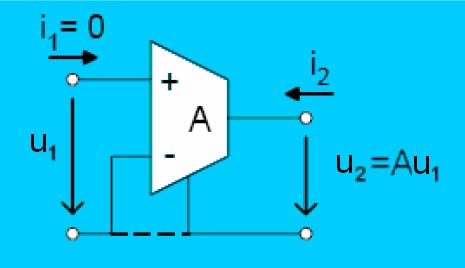
\includegraphics[width=0.7\linewidth]{Obrazky/AE1/VCVS}
		\caption[Riadené zdroje]{VCVS}
		\label{fig:VCVS}
	\end{subfigure}
	\begin{subfigure}[b]{0.45\textwidth}
		\centering
		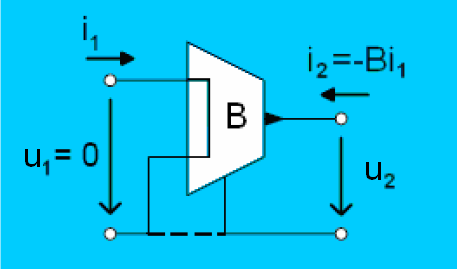
\includegraphics[width=0.7\linewidth]{Obrazky/AE1/CCCS}
		\caption[Riadené zdroje]{CCCS}
		\label{fig:CCCS}
	\end{subfigure}
	\begin{subfigure}[b]{0.45\textwidth}
		\centering
		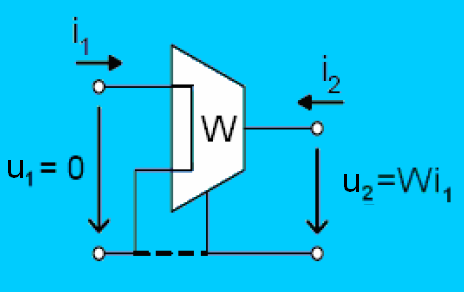
\includegraphics[width=0.7\linewidth]{Obrazky/AE1/CCVS}
		\caption[Riadené zdroje]{CCVS}
		\label{fig:CCVS}
	\end{subfigure}
	\begin{subfigure}[b]{0.45\textwidth}
		\centering
		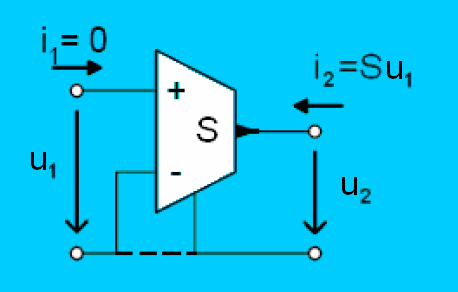
\includegraphics[width=0.7\linewidth]{Obrazky/AE1/VCCS}
		\caption[Riadené zdroje]{VCCS}
		\label{fig:VCCS}
	\end{subfigure}
	\caption{Štyri základné riadené zdroje}
	\label{fig:riadenezdroje}
\end{figure}
Popis k \ref{fig:riadenezdroje}
\begin{itemize}
	\item \ref{fig:VCVS} - Voltage Controled Voltage Source - Napäťovo riadený napäťový zdroj
	(Klasický OZ - OPA - Napäťový zosilňovač)
	\item \ref{fig:CCCS} - Current Controled Current Source - Prúdovo riadený prúdový zdroj
	(Prúdový zosilňovač)
	\item \ref{fig:CCVS} - Current Controled Voltage Source - Prúdovo riadený napäťový zdroj
	
	\item \ref{fig:VCCS} - Voltage Controled Current Source - Napäťovo riadený prúdový zdroj
	(Transkonduktančný zosilňovač - OTA)
\end{itemize}
\emph{Treba sa zamerať na jednotlivé prenosy a~značky blokov, ktoré sú vyznačené v obrázkoch na \ref{fig:riadenezdroje}}.

\section{Imitančný invertor a konvertor}
\subsubsection{Imitančný invertor}
Lineárny dvojbran. Jeho bránové prenosy sú viazané opačne, resp. inverzne. Prenosy sú nezávislé od vonkajšieho zapojenia.
\begin{figure}[H]
	\centering
	\begin{subfigure}[b]{0.65\textwidth}
		\centering
		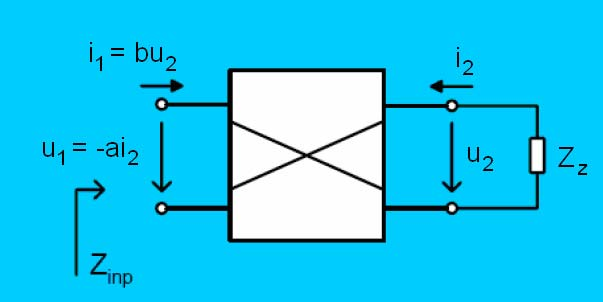
\includegraphics[width=0.6\linewidth]{Obrazky/AE1/imitInvert}
		\caption{Imitančný invertor}
		\label{fig:imitInvert}
	\end{subfigure}
	\begin{subfigure}[b]{0.3\textwidth}
		\centering
		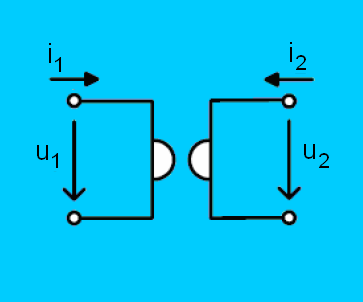
\includegraphics[width=0.7\linewidth]{Obrazky/AE1/gyrator}
		\caption{Špeciálny prípad Imitančného invertora - Gyrátor}
		\label{fig:gyrator}
	\end{subfigure}
	\label{fig:imitGyr}
	\caption{Imitančný invertor a gyrátor}
\end{figure}
Invertor transformuje zaťažovaciu impedanciu $Z_Z$ na vstupnú bránu, viz \ref{fig:imitInvert}. Pričom platí, že: 
\begin{equation}
	Z_{inp} = \frac{a}{b}\frac{1}{Z_Z} = k \cdot \frac{1}{Z_Z} \\
\end{equation}
Teda vstupná impedancia je úmerná inverznej hodnote zaťažovacej $Z_Z$. Podľa znamienka $k$, rozlišujeme medzi \emph{pozitívnym} a~\emph{negatívnym} invertorom $\implies$, \underline{$k > 0$ pozitívny, $k < 0$ negatívny invertor}.

\underline{Gyrátor \ref{fig:gyrator}, je pozitívny imitačný invertor} - Používa sa pri návrhu aktívnych RC filtrov a vyrába sa ako integrovaný obvod. Väčšinou býva symetrický.
Pri kapacitnej záťaži imituje induktívny charakter impedancie na vstupnej bráne. Pričom pre kapacitnú záťaž platí:
\begin{equation}
	Z_{inp} = k \cdot sC = s\cdot L_{ekv}
\end{equation}

\subsubsection{Imitačný konvertor}
Znovu lineárny dvojbran \ref{fig:imitKonvert}, Transformuje zaťažovaciu impedanciu na vstupnú bránu, s koeficientom $k$. Platí:
\begin{equation}
	Z_{inp} = \frac{a}{b}Z_Z = k \cdot Z_Z
\end{equation}
\begin{figure}[H]
	\centering
	\begin{subfigure}[b]{0.65\textwidth}
		\centering
		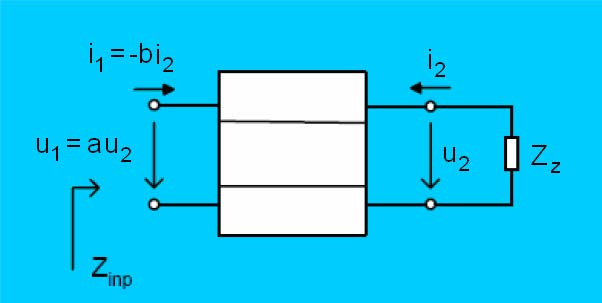
\includegraphics[width=0.6\linewidth]{Obrazky/AE1/imitKonvert}
		\caption{Imitančný konvertor}
		\label{fig:imitKonvert}
	\end{subfigure}
	\begin{subfigure}[b]{0.3\textwidth}
		\centering
		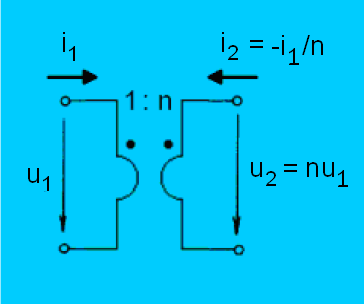
\includegraphics[width=0.7\linewidth]{Obrazky/AE1/idealTransform}
		\caption{Ideálny transformátor}
		\label{fig:idealTransform}
	\end{subfigure}
	\label{fig:konvTrans}
	\caption{Imitančný konvertor a ideálny transformátor}
\end{figure}

Podľa znamienka $k$, rozlišujeme medzi \emph{pozitívnym} \newline a~\emph{negatívnym} konvertorom $\implies$, \underline{$k > 0$ pozitívny, $k < 0$ negatívny konvertor}. Používa sa k získaniu záporného odporu. Prvok ako taký je neregurálny $\implies$ nedá sa popísať imitančnými parametrami (z imitančnej matice).

Obrázok \ref{fig:idealTransform} zobrazuje ideálny transformátor, čo je typ pozitívneho konvertora, kedy je zaťažovacia impedancia transformovaná na vstupnú bránu s kvadrátom, platí:
\begin{align}
	a &= \frac{1}{n} \\
	b &= n \\
	Z_{inp} &= \frac{1}{n^2} Z_Z
\end{align}

\section{Ideálny a reálny OZ}
\subsubsection{Ideálny OZ - (IOZ)}
Neregulárny dvojbran, považuje sa za limitný prípad ideálneho napäťového a prúdového zosilňovača, pričom zosilnenie ideálneho OZ je $\text{A} \rightarrow \infty$ a $\text{B} \rightarrow \infty$. Jeho vstupná impedancia je nekonečná a výstupná zase nulová. 

Podľa počtu vstupov vieme rozdeliť na:
\begin{description}
	\item[SISO] Single Input Single Output - nevyrába sa, realizuje sa z DISO - výstup skratneš s invertujúcim vstupom a vznikne buffer
	\item[DISO] Double Input Single Output - nazýva sa napäťový, najrozšírenejší OZ, všade ho dostať
	\item[SIDO] Single Input Double Output - duálne DISO, prúdový OZ, používa sa pre neivertujúci prúdový sledovač / zosilňovač
	\item[DIDO] Double Input Double Output - nazýva sa plávajúci, diferenciálny vstup a diferenciálny výstup, typický pre transimpedančný zosilňovač
\end{description}
\emph{Diferenciálny - symetrický, Single - nesymetrický}

\subsubsection{Reálny OZ}
Reálny OZ má obmedzené hodnoty zosilnenia, $A_0 \approx 10^5$, jeho vstupná impedancia je rovnako konečná, pričom výstupná je nenulová. Nakoľko sa jedná o reálnu štruktúru, má aj parazitné javy:
\begin{multicols}{2}
	\begin{itemize}
		\item offset, medzi vstupmi $U_{IO}$, závisí na teplotnom a časovom drifte či na prieniku napájacieho napätia - jeho kolísaniu
		\item prúdová nesymetria vstupov,
		\item vstupný odpor (impedancia),
		\item frekvenčná závislosť zosilnenia $A$,
		\item drift (utekanie $U_{IO}$),
		\item vstupné zvyškové prúdy,
		\item výstupný odpor (impedancia).
	\end{itemize}
\end{multicols}

Pri OZ sa udáva frekvenčná (modulová) a pracovná charakteristika. \newline
\underline{Pracovná charakteristika \ref{fig:pracovnaChar}}
Vzťah medzi vstupným a výstupným napätím - strmosť predstavuje zosilnenie. Obsahuje okrajové časti - vrchná a spodná limitácia (saturácia z napájacieho napätia), a stredná časť - aktívna oblasť. Stred aktívnej oblasti neprechádza nulou ale prechádza offsetom / nesymetriou.

\underline{Modulová charakteristika \ref{fig:modulChar}}
Štandardná charakteristika udaná jedným pólom, odpovedá prenosovej funkcii:
\begin{equation}
	A(s) = \frac{A_0 \omega_0}{s + \omega_0}
\end{equation}
Pričom $\omega_0$ odpovedá \qty{-3}{\dB} - teda je to \underline{medzná frekvencia}, $\omega_t$ je \underline{tranzientná frekvencia} - keď zisk $A = 0 \; \unit{dB}$.

\begin{figure}[H]
	\centering
	\begin{subfigure}[b]{0.45\textwidth}
		\centering
		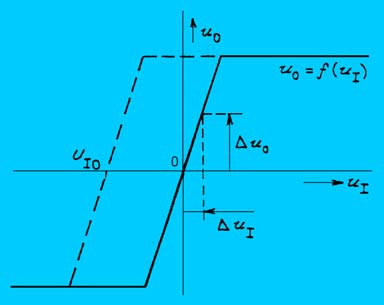
\includegraphics[width=0.7\linewidth]{Obrazky/AE1/pracovnaChar}
		\caption{Pracovná charakteristika OZ}
		\label{fig:pracovnaChar}
	\end{subfigure}
	\begin{subfigure}[b]{0.45\textwidth}
		\centering
		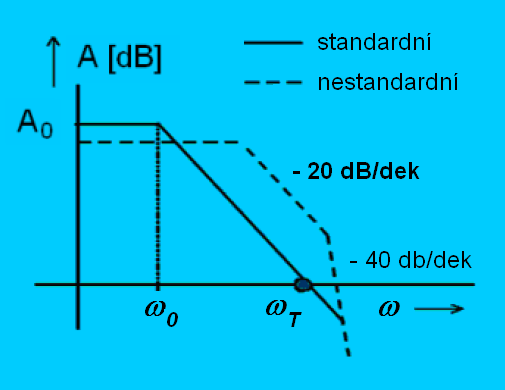
\includegraphics[width=0.7\linewidth]{Obrazky/AE1/modulchar}
		\caption{Modulová charakteristika OZ}
		\label{fig:modulChar}
	\end{subfigure}
	\label{fig:OZChar}
	\caption{Charakteristiky OZ}
\end{figure}

\section{Prúdový konvejor}
Funkčné mnohobrany, ktorých vzťahy sú medzi bránami sú rôzne definované bránovými veličinami. \underline{Konvejorovaním} sa rozumie sledovanie U a I, je možná aj inverzia. Konvejor \ref{fig:konvejor} dosahuje lepšie frekvenčné vlastnosti ako štandardný OZ - pracuje v prúdovom móde.
\begin{figure}[htpb]
	\centering
	% --- ĽAVÁ STRANA: OBRÁZOK ---
	\begin{minipage}[c]{0.35\textwidth}
		\centering
		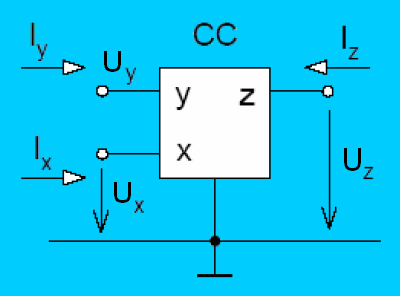
\includegraphics[width=\linewidth]{Obrazky/AE1/konvejor}
		\caption{Trojbránový konvejor typu CCII+}
		\label{fig:konvejor}
	\end{minipage}
	\hfill % Vyplní medzeru medzi minipages
	% --- PRAVÁ STRANA: TEXT A ROVNICE ---
	\begin{minipage}[c]{0.60\textwidth}
		Pre vzťahy medzi bránovými veličinami platí:
		\begin{align*}
			U_x &= U_y \\
			I_y &= 0 \\
			I_z &= I_x 
		\end{align*}
		Obecne platí:
		\begin{equation*}
			\begin{aligned}
				U_x &= aU_y \\
				I_y &= bI_x \\
				I_z &= cI_x 
			\end{aligned}
			\,\implies\,
			\begin{pmatrix} U_x \\ I_y \\ I_z \end{pmatrix} = 
			\begin{pmatrix} 
				a & 0 & 0 \\ 
				0 & b & 0 \\ 
				0 & c & 0 
			\end{pmatrix} 
			\begin{pmatrix} U_y \\ I_x \\ I_x \end{pmatrix}
		\end{equation*}
	\end{minipage}
\end{figure}
\subsubsection{Rozdelenie Konvejorov}
\emph{Asi netreba ale len pre úplnosť}
\begin{description}
	\item[Koeficient $a = \{+1, -1\}$] (Smer/polarita prenosu napätia)
	\begin{description}
		\item[$+1$:] \textbf{CC (neinvertujúci)} -- napätie sa prenáša bez zmeny polarity.
		\item[$-1$:] \textbf{ICC (invertujúci)} -- napätie sa na výstupe invertuje.
	\end{description}
	
	\item[Koeficient $b = \{+1, 0, -1\}$] (Generácie prúdových konvejorov)
	\begin{description}
		\item[$+1$:] \textbf{CCI (1. generácia, 1968)} -- prvá verzia prúdového konvejoru.
		\item[$\phantom{+}0$:] \textbf{CCII (2. generácia, 1970)} -- druhá, najpoužívanejšia generácia (autori Sedra \& Smith).
		\item[$-1$:] \textbf{CCIII (3. generácia, 1995)} -- tretia generácia (autor Fabre).
	\end{description}
	
	\item[Koeficient $c = \{+1, -1\}$] (Smer/polarita výstupného prúdu)
	\begin{description}
		\item[$+1$:] \textbf{CC+ (pozitívny)} -- výstupný prúd tečie rovnakým smerom (pozitívna polarita).
		\item[$-1$:] \textbf{CC- (negatívny)} -- výstupný prúd tečie opačným smerom (negatívna polarita).
	\end{description}
\end{description}

\section{Typické zapojenia s OZ}
\subsubsection{Zapojenia s napäťovým zosilňovačom}
\begin{figure}[H]
	\centering
	\begin{subfigure}[b]{0.45\textwidth}
		\centering
		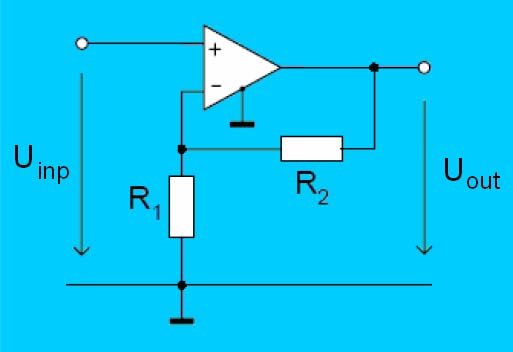
\includegraphics[width=0.6\linewidth]{Obrazky/AE1/zosikPlus}
		\caption{Neinvertujúci zosilňovač}
		\label{fig:zos}
	\end{subfigure}
	\begin{subfigure}[b]{0.45\textwidth}
		\centering
		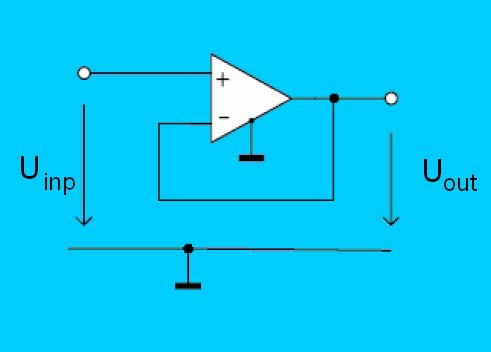
\includegraphics[width=0.6\linewidth]{Obrazky/AE1/buufer}
		\caption{Buffer - sledovač}
		\label{fig:buffer}
	\end{subfigure}
	\begin{subfigure}[b]{0.45\textwidth}
		\centering
		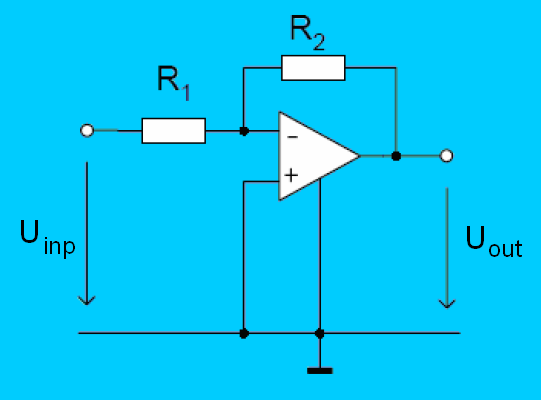
\includegraphics[width=0.6\linewidth]{Obrazky/AE1/zosikMinus}
		\caption{Invertujúci zosilňovač}
		\label{fig:zosInvert}
	\end{subfigure}
	\begin{subfigure}[b]{0.45\textwidth}
		\centering
		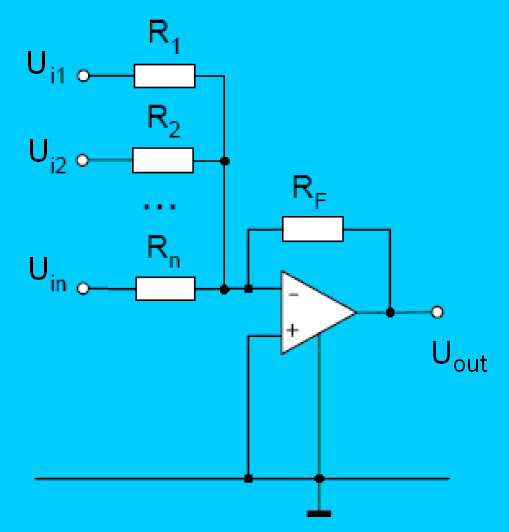
\includegraphics[width=0.5\linewidth]{Obrazky/AE1/sumator}
		\caption{Sumačný zosilňovač}
		\label{fig:sumator}
	\end{subfigure}
	\caption{Štyri základné zapojenia s Napäťovým OZ}
	\label{fig:zapojeniaNapatoveOZ}
\end{figure}
Na obrázku \ref{fig:zapojeniaNapatoveOZ} sú uvedené typické zapojenie s využitím napäťového zosilňovača. Pre neinvertujúci zosilňovač, obrázok \ref{fig:zos}, platí prenos:
	\begin{align*}
		\text{Ideálny prípad } (A \to \infty): \quad K_U &= 1 + \frac{R_2}{R_1} 
		& 
		\text{Reálny OZ: } \quad K_U &= \frac{A(R_1 + R_2)}{R_1(A + 1) + R_2}
	\end{align*}
Modifikáciou na buffer (vytvoríme SISO) obrázok \ref{fig:buffer}, dosiahneme: 
\begin{equation*}
	K_U = \frac{U_{out}}{U_{in}} = 1
\end{equation*}
Inverujúci napäťový zosilňovač, obrázok \ref{fig:zosInvert}:
\begin{align}
	\text{Ideálny prípad: } \quad K_U &= -\frac{R_2}{R_1} 
	& 
	\text{Reálny OZ: } \quad K_U &= \frac{-AR_2}{R_1(A + 1) + R_2}
	\label{eqv:invertOZPrenos}
\end{align}
Kedy narozdiel od prechádzajúcich zapojení je pri \ref{fig:zosInvert}, vstupná impedancia daná $R_1$ a prúd na vstupne je nenulový.

Obrázky \ref{fig:zos}, \ref{fig:buffer} a \ref{fig:zosInvert}. Boli asi veľmi jednoduché tak si niekto vymyslel sumátor napätia, obrázok \ref{fig:sumator}. Výstup je daný:
\begin{equation}
	U_{out} = - \left( \frac{R_F}{R_1} U_{i1} + \frac{R_F}{R_2} U_{i2} + \dots + \frac{R_F}{R_n} U_{in} \right)
\end{equation}
\emph{Existujú aj zložitejšie zapojenia s využitím rozsiahlejších odporových sietí, každé má inú prenosovú funkciu.}

\subsubsection{Zapojenia s prúdovým zosilňovačom}
Prúdový zosilňovač sa dá vytvoriť výmenou vstupov za výstupy pri DISO - vieme tak dosiahnuť SIDO. V obvodoch je realizovaná záporná prúdová paralelná spätná väzba (Delič $R_1$ a $R_2$ v obrázku \ref{fig:zosPrud}), teda časť vstupného prúdu sa privádza do výstupnej brány.
\begin{figure}[H]
	\centering
	\begin{subfigure}[b]{0.45\textwidth}
		\centering
		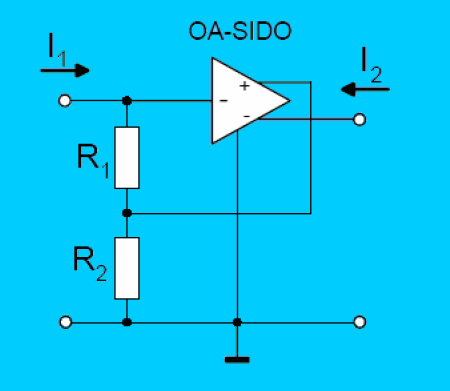
\includegraphics[width=0.55\linewidth]{Obrazky/AE1/zosPrud}
		\caption{Prúdový zosilňovač}
		\label{fig:zosPrud}
	\end{subfigure}
	\begin{subfigure}[b]{0.45\textwidth}
		\centering
		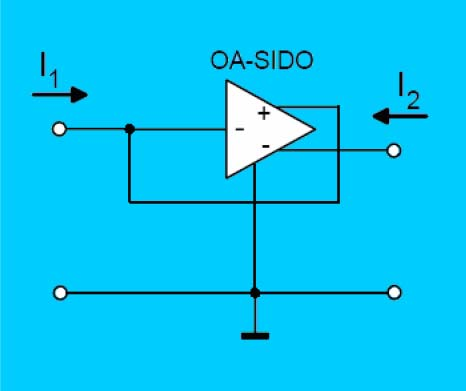
\includegraphics[width=0.55\linewidth]{Obrazky/AE1/bufferPrud}
		\caption{Prúdový sledovač}
		\label{fig:bufferPrud}
	\end{subfigure}
	\label{fig:zapojeniaPrudove}
	\caption{Zapojenia prúdových zosilňovačov}
\end{figure}
Platí: 
\begin{equation}
	K_I = \frac{-I_2}{I_1} = 1 + \frac{R_1}{R_2}
\end{equation}
Jedná sa o duálny vzťah k \ref{eqv:invertOZPrenos}. Rovnako je vstupná impedancia nulová a teda aj vstupné napätie???

\subsubsection{Prevodník prúd - napätie}
\begin{figure}[H]
	\centering
	% --- ĽAVÁ STRANA: OBRÁZOK ---
	\begin{minipage}[c]{0.35\textwidth}
		\centering
		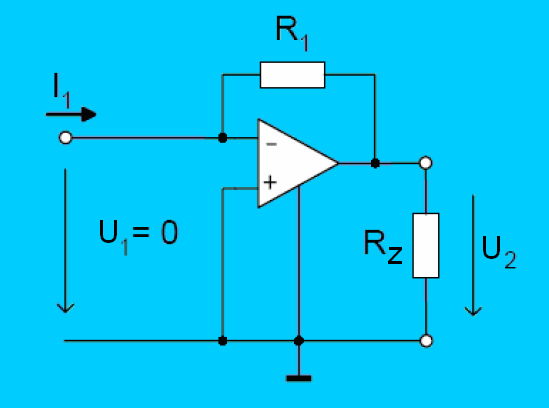
\includegraphics[width=\linewidth]{Obrazky/AE1/prevodnikUI}
		\caption{Prevodník prúdu na napätie}
		\label{fig:prevodnikIU}
	\end{minipage}
	\hfill % Vyplní medzeru medzi minipages
	% --- PRAVÁ STRANA: TEXT A VZORCE ---
	\begin{minipage}[c]{0.60\textwidth}
		Zapojenie na obrázku \ref{fig:prevodnikIU} sa nazýva prevodník prúd -- napätie, alebo aj transrezistor (má tzv. transimpedanciu $Z_T$). Dá sa realizovať aj z SISO. Pre transimpedanciu $Z_T$ tohto prevodníka platí:
		
		\begin{align*}
			\text{Reálny OZ: } \ Z_T &= \frac{U_2}{I_1} = -\frac{R_1 A}{1 + A} \\
			\text{Ideálny OZ } (A \to \infty): \ Z_T &= \frac{U_2}{I_1} = -R_1
		\end{align*}
	\end{minipage}
\end{figure}
\subsubsection{Prevodník napätie - prúd}
Nazýva sa transkonduktor, jeho realizácia záleží od typu záťaže - oddelená či zemnená.
\begin{figure}[H]
	\centering
	\begin{subfigure}[b]{0.45\textwidth}
		\centering
		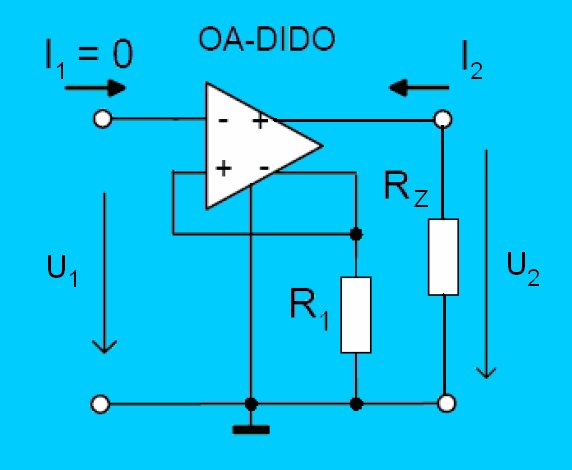
\includegraphics[width=0.55\linewidth]{Obrazky/AE1/didoUI}
		\caption{U/I prevodník s DIDO}
		\label{fig:prevodnikUIdido}
	\end{subfigure}
	\begin{subfigure}[b]{0.45\textwidth}
		\centering
		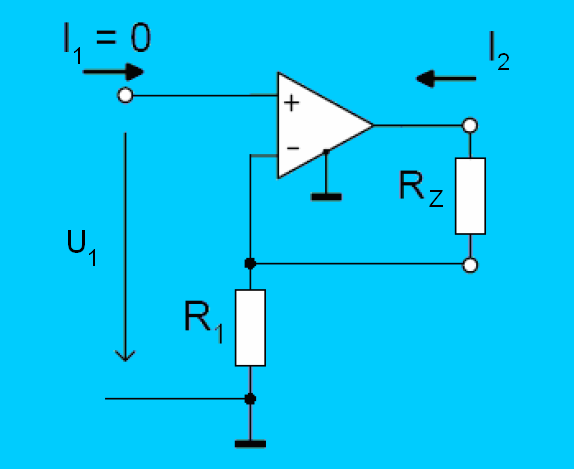
\includegraphics[width=0.55\linewidth]{Obrazky/AE1/disoUI}
		\caption{U/I prevodník s DISO}
		\label{fig:prevodnikUIdiso}
	\end{subfigure}
	\label{fig:zapojeniaUIprevodnikov}
	\caption{Zapojenia prevodníkov napätie - prúd}
\end{figure}
Obvod má nasledujúce parametre:
\begin{equation}
	I_1 = 0 \quad \text{(a)}, \qquad -I_2 = Y_T U_1 \quad \text{(b)}, \qquad Y_T = \frac{-I_2}{U_1} = -\frac{1}{R_1} \quad \text{(c)}
\end{equation}

Prevodník $U \to I$ s plávajúcou záťažou ($R_Z$) je možné jednoduchšie realizovať s OZ-DISO. Pre transkonduktanciu $Y_T$ tohto prevodníka platí:

\begin{align*}
	\text{Reálny OZ: } \quad Y_T &= \frac{-I_2}{U_1} = \frac{A}{R_Z + R_1(1 + A)}
	&
	\text{Ideálny prípad } (A \to \infty): \quad Y_T &= \frac{1}{R_1}
\end{align*}

Vstupná a výstupná impedancia oboch vyššie uvedených transkonduktorov sú v ideálnom prípade nekonečné.
\newpage
\chapter{Analógové elektrické filtre}
Frekvenčné filtre sú lineárne dvojbrany. Ich účel je jasný - prepustia len isté frekvenčné pásmo, zvyšné pásmo je potláčané. Filtre sa delia podľa:
\begin{itemize}
	\item prenášanáho pásma (Dolná priepusť, Horná priepusť, Pásmová priepusť, Pásmová zádrž)
	\item tvaru frekvenčnej charakteristiky
	\item rádu prenosovej funkcie
	\item použitých prvkov (RC, LC/RLC, aktívne R, syntetické (s gyrátorom), SAW)
\end{itemize}


\section{Pasívne filtre}
\subsubsection{Prvého rádu}
Pasívne filtre sú v podstate frekvenčne závislé deliče - teda v najzákladnejšej podobe (RC, CR 1. rádu)

\begin{figure}[H]
	\centering
	\begin{subfigure}[b]{0.45\textwidth}
		\centering
		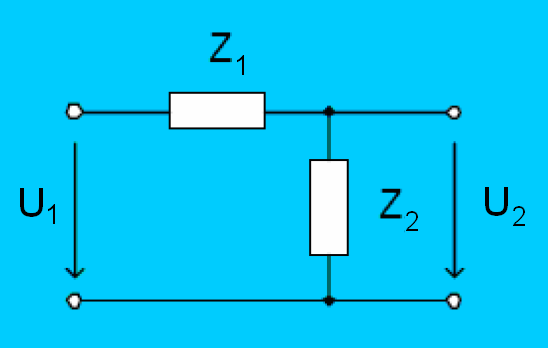
\includegraphics[width=0.6\linewidth]{Obrazky/AE1/druhaOtazka/frekZZ}
		\caption{Frekvenčne závislý delič napätia}
		\label{fig:frekZZ}
	\end{subfigure}
	\begin{subfigure}[b]{0.45\textwidth}
		\centering
		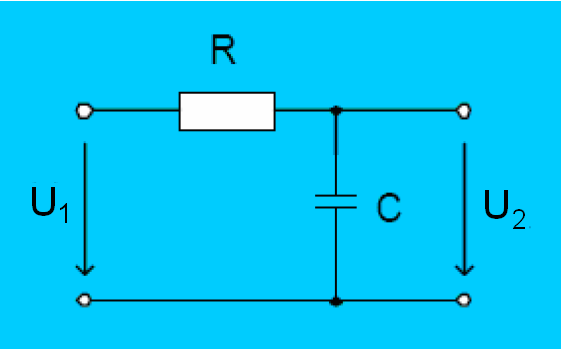
\includegraphics[width=0.6\linewidth]{Obrazky/AE1/druhaOtazka/RC}
		\caption{RC filter - 1 rád - dolná priepusť}
		\label{fig:RC}
	\end{subfigure}
	\begin{subfigure}[b]{0.45\textwidth}
		\centering
		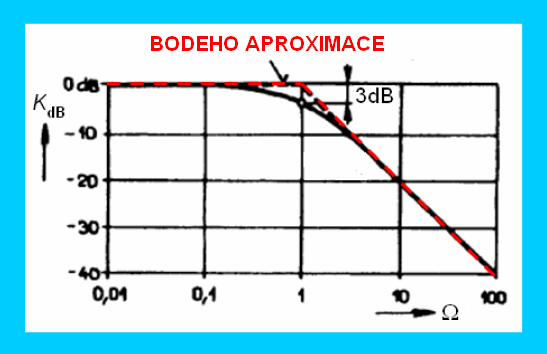
\includegraphics[width=0.6\linewidth]{Obrazky/AE1/druhaOtazka/RCfrek}
		\caption{Frekvenčná / Modulová charakteristika}
		\label{fig:RCfrek}
	\end{subfigure}
	\begin{subfigure}[b]{0.45\textwidth}
		\centering
		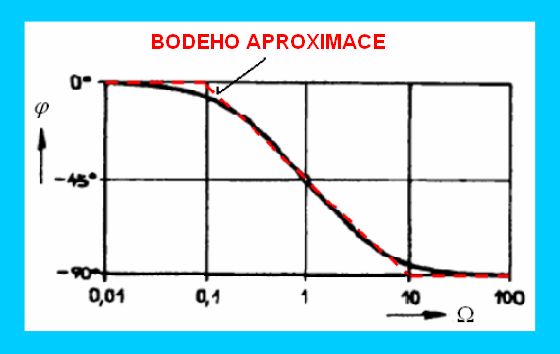
\includegraphics[width=0.6\linewidth]{Obrazky/AE1/druhaOtazka/RCfaza}
		\caption{Fázová / Argumentová charakteristika}
		\label{fig:RCfaza}
	\end{subfigure}
	\caption{Základný polčlánok - frekvenčne závislý delič}
	\label{fig:RCpvehoradu}
\end{figure}
Uvažujme dolný priepust RC ako príklad pasívneho filtra 1. rádu. Po dosadení za príslušné impedancie dostávame pre prenosovú funkciu vzťah:
\begin{equation}
	\mathbf{K}(j\omega) = \frac{1 / j\omega C}{R + 1 / j\omega C} = \frac{1}{1 + j\omega RC}
\end{equation}

Modulová charakteristika \ref{fig:RCfrek} tohto obvodu je potom daná vzťahom:
\begin{equation}
	K(\omega) = |\mathbf{K}(j\omega)| = \frac{1}{\sqrt{1 + \omega^2 R^2 C^2}}
\end{equation}

Zisk v decibeloch je rovný:
\begin{equation}
	k(\omega) = K_{\text{dB}}(\omega) = 20 \log K(\omega)
\end{equation}

Argumentová (fázová) \ref{fig:RCfaza} charakteristika je daná vzťahom:
\begin{equation}
	\varphi(\omega) = \arg \mathbf{K}(j\omega) = -\arctan \omega RC
\end{equation}
Medzný kmitočet $\omega_m$ je definovaný poklesom zisku o \SI{-3}{dB} (argument je rovný \SI{-45}{^\circ}):
\begin{equation}
	K(\omega_m) = \frac{K_0}{\sqrt{2}} \quad (\text{kde } K_0 = 1), \qquad K_{\text{dB}}(\omega_m) = K_{0\text{dB}} - 3
\end{equation}

V tomto obvode je daný vzťahom:
\begin{equation}
	\omega_m = \frac{1}{\tau} = \frac{1}{RC} \implies f_m = \frac{1}{2 \pi \cdot R C}
\end{equation}

Na medznom kmitočte nastáva zmena v sklone asymptot pri Bodeho aproximácii modulovej charakteristiky (s maximálnou odchýlkou \SI{3}{dB} od skutočnej). Pri fázovej charakteristike sú zlomy dva (dekádu pred a dekádu po $\omega_m$, s maximálnou odchýlkou \SI{5.7}{^\circ}).

Pre jednoduchší návrh zavádzame normované kmitočtové premenné:
\begin{equation}
	p = \frac{s}{\omega_N}, \qquad \Omega = \frac{\omega}{\omega_N}
\end{equation}

Najčastejšie normujeme k medznému kmitočtu $\omega_N = \omega_m$. Obvodové funkcie dolného priepustu 1. rádu sú potom v normovanom tvare:
\begin{equation}
	K(p) = \frac{1}{1 + p}, \qquad K(\Omega) = \frac{1}{\sqrt{1 + \Omega^2}}, \qquad \varphi(\Omega) = -\arctan\Omega
\end{equation}
\subsubsection{Druhého rádu}
Vyššiu strmosť frekvenčnej charakteristiky \ref{fig:RCfrek} vieme dosiahnuť zvýšením rádu filtra. Pre \ref{fig:RC} to dosiahneme náhradou R za L - vznikne R + L v sérií, R vyjadruje straty na L, dostaneme dolnú prepusť 2. rádu. Prenosové funkcie vyzerajú nasledovne:
Pre tento obvod je možné odvodiť napäťový prenos vo všeobecnom tvare:
\begin{equation}
	K(s) = \frac{a_0}{b_2 s^2 + b_1 s + b_0} = \frac{K_0}{LCs^2 + RCs + 1} = \frac{K_0 \omega_p^2}{s^2 + \frac{\omega_p}{Q_p} s + \omega_p^2}
\end{equation}

Póly sú komplexne združené ($\operatorname{Im} p_1 = -\operatorname{Im} p_2$), ich frekvencia je:
\begin{equation}
	\omega_p = \frac{1}{\sqrt{LC}}
\end{equation}

a činiteľ kvality je daný vzťahom (činiteľ kvality hovorí o veľkosti prekmitu na lomovej frekvencii):
\begin{equation}
	Q_p = \frac{\omega_p}{2\sigma_p} = \frac{\omega_p L}{R}
\end{equation}

Uhlová frekvencia $\omega_d$, vyznačená na imaginárnej osi, vyjadruje vlastný kmitočet oscilácií.

% --- PRENOSOVÉ FUNKCIE VEDĽA SEBA ---
\begin{align*}
	\text{Dolná priepust (LP): } \quad K(s) &= \frac{K_0 \omega_p^2}{s^2 + \frac{\omega_p}{Q_p} s + \omega_p^2}
	&
	\text{Horná priepust (HP): } \quad K(s) &= \frac{K_0 s^2}{s^2 + \frac{\omega_p}{Q_p} s + \omega_p^2}
\end{align*}
Hornú priepusť 2. rádu vieme realizovať zámenou C za R + L.
\begin{figure}[H]
	\centering
	\begin{subfigure}[b]{0.28\textwidth}
		\centering
		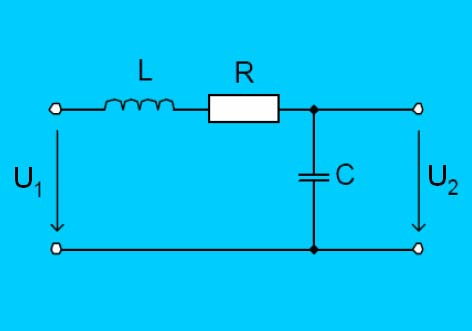
\includegraphics[width=0.8\linewidth]{Obrazky/AE1/druhaOtazka/LRC}
		\caption{Dolná priepusť 2. rádu}
		\label{fig:LRC}
	\end{subfigure}
	\begin{subfigure}[b]{0.28\textwidth}
		\centering
		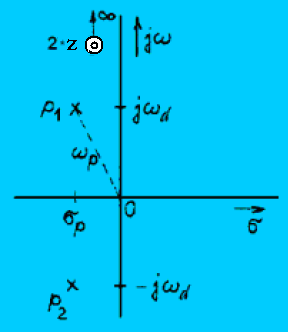
\includegraphics[width=0.55\linewidth]{Obrazky/AE1/druhaOtazka/LRCnula}
		\caption{rozloženie pólov a núl}
		\label{fig:LRCnula}
	\end{subfigure}
	\begin{subfigure}[b]{0.28\textwidth}
		\centering
		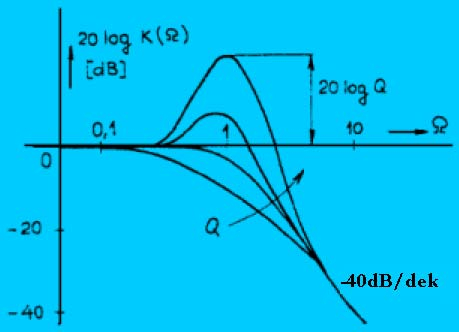
\includegraphics[width=0.8\linewidth]{Obrazky/AE1/druhaOtazka/LRCmodul}
		\caption{modulová charakteristika}
		\label{fig:LRCmodul}
	\end{subfigure}
	\label{fig:LRCdolna}
	\caption{Dolná priepusť 2. rádu}
\end{figure}
\begin{figure}[H]
	\centering
	\begin{subfigure}[b]{0.28\textwidth}
		\centering
		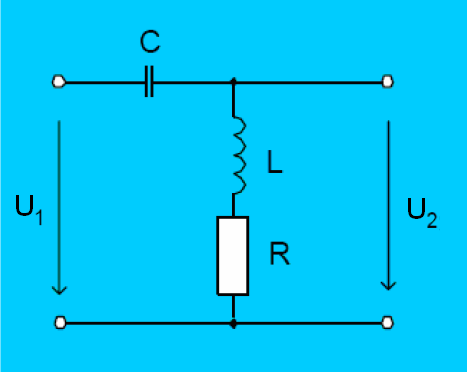
\includegraphics[width=0.8\linewidth]{Obrazky/AE1/druhaOtazka/CLR}
		\caption{Horná priepusť 2. rádu}
		\label{fig:CLR}
	\end{subfigure}
	\begin{subfigure}[b]{0.28\textwidth}
		\centering
		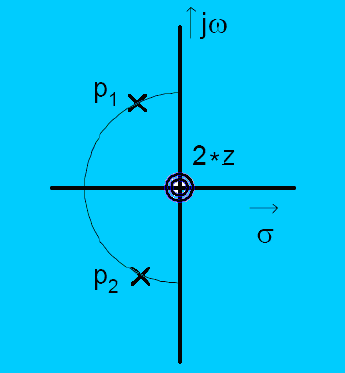
\includegraphics[width=0.55\linewidth]{Obrazky/AE1/druhaOtazka/CLRnula}
		\caption{rozloženie pólov a núl}
		\label{fig:CLRnula}
	\end{subfigure}
	\begin{subfigure}[b]{0.28\textwidth}
		\centering
		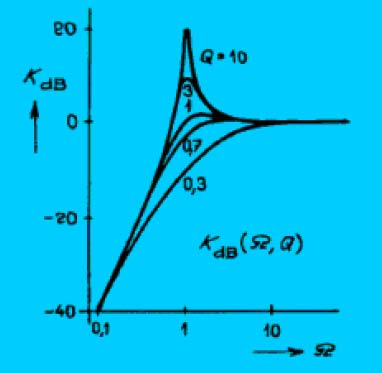
\includegraphics[width=0.8\linewidth]{Obrazky/AE1/druhaOtazka/CLRmodul}
		\caption{modulová charakteristika}
		\label{fig:CLRmodul}
	\end{subfigure}
	\label{fig:CLRhorna}
	\caption{Horná priepusť 2. rádu}
\end{figure}
\subsubsection{Pásmové Priepuste / Zádrže}
\begin{figure}[H]
	\centering
	\begin{subfigure}[b]{0.28\textwidth}
		\centering
		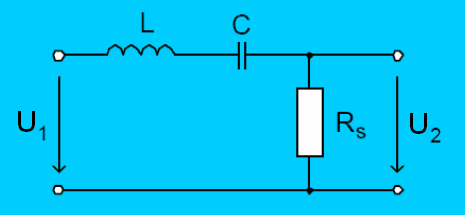
\includegraphics[width=0.8\linewidth]{Obrazky/AE1/druhaOtazka/PPRS}
		\caption{Realizácia pásmovej priepuste 2. rádu}
		\label{fig:PPRS}
	\end{subfigure}
	\begin{subfigure}[b]{0.28\textwidth}
		\centering
		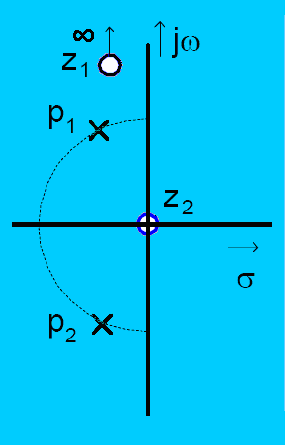
\includegraphics[width=0.55\linewidth]{Obrazky/AE1/druhaOtazka/PPnula}
		\caption{rozloženie pólov a núl}
		\label{fig:PPnula}
	\end{subfigure}
	\begin{subfigure}[b]{0.28\textwidth}
		\centering
		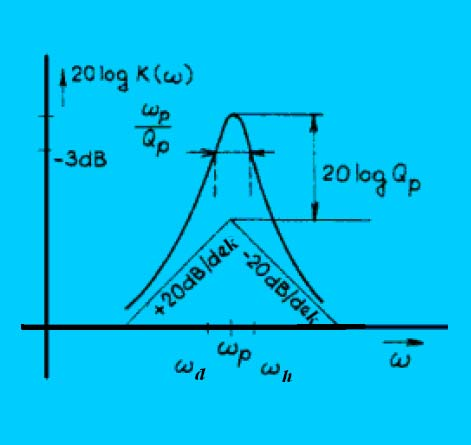
\includegraphics[width=0.8\linewidth]{Obrazky/AE1/druhaOtazka/PPmodul}
		\caption{modulová charakteristika}
		\label{fig:PPmodul}
	\end{subfigure}
	\label{fig:PP}
	\caption{Pásmová priepusť 2. rádu}
\end{figure}
\begin{figure}[H]
	\centering
	\begin{subfigure}[b]{0.28\textwidth}
		\centering
		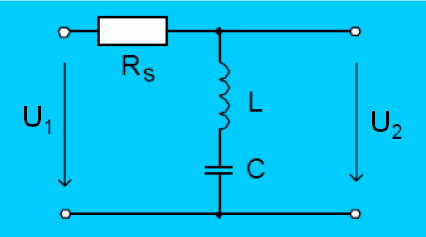
\includegraphics[width=0.8\linewidth]{Obrazky/AE1/druhaOtazka/PZRS}
		\caption{Pásmová zádrž 2. rádu}
		\label{fig:PZRS}
	\end{subfigure}
	\begin{subfigure}[b]{0.28\textwidth}
		\centering
		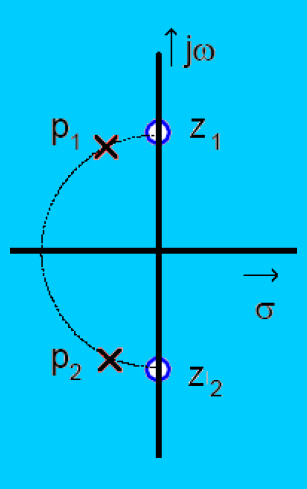
\includegraphics[width=0.55\linewidth]{Obrazky/AE1/druhaOtazka/PZnula}
		\caption{rozloženie pólov a núl}
		\label{fig:PZRSnula}
	\end{subfigure}
	\begin{subfigure}[b]{0.28\textwidth}
		\centering
		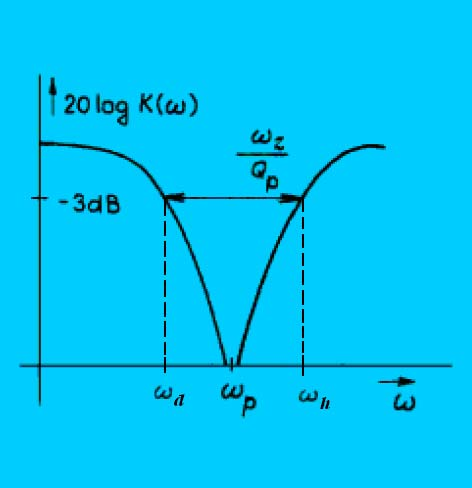
\includegraphics[width=0.8\linewidth]{Obrazky/AE1/druhaOtazka/PZmodul}
		\caption{modulová charakteristika}
		\label{fig:PZRSmodul}
	\end{subfigure}
	\caption{Pásmová zádrž 2. rádu}
	\label{fig:PZ}
\end{figure}
Prenosová funkcia pásmovej priepuste (PP) a pásmovej zádrže (PZ) vo všeobecnom tvare:
\begin{align*}
	\text{Pásmová priepusť (PP): } \quad K(s) &= \frac{a_1 s}{b_2 s^2 + b_1 s + b_0} = \frac{K_0 \frac{\omega_p}{Q_p} s}{s^2 + \frac{\omega_p}{Q_p} s + \omega_p^2} \\
	\text{Pásmová zádrž (PZ): } \quad K(s) &= \frac{a_2 s^2 + a_0}{b_2 s^2 + b_1 s + b_0} = K_0 \frac{s^2 + \omega_p^2}{s^2 + \frac{\omega_p}{Q_p} s + \omega_p^2} \quad \Longleftarrow \quad \omega_z = \omega_p
\end{align*}
Parametre pásmovej priepuste (PP) sú dané nasledovne:
\begin{equation}
	\omega_p = \omega_{\text{rez}} = \frac{1}{\sqrt{LC}}, \qquad Q_p = \frac{\omega_p L}{R_s} = \frac{R_p}{\omega_p L},\qquad B_\omega = \omega_h - \omega_d = \frac{\omega_p}{Q_p}
\end{equation}
\underline{Všeobecný obvod 2. rádu sa nazýva bikvád - bikvadratická štruktúra.} Jeho prenosová funkcia je nižšie. Platí, že $\omega_p = \omega_z$. Teda Póly a Nuly ležia v imaginárnej rovine na jednej kružnici \ref{fig:PZRSnula}. Pásmová zádrž \ref{fig:PZ} spĺňa podmienky pre bikvád.
\begin{equation}
	K(s) = \frac{a_2 s^2 + a_1 s + a_0}{b_2 s^2 + b_1 s + b_0} = K_0 \frac{(s - z_1)(s - z_2)}{(s - p_1)(s - p_2)} = K_0 \frac{s^2 + \frac{\omega_z}{Q_z} s + \omega_z^2}{s^2 + \frac{\omega_p}{Q_p} s + \omega_p^2} \ .
\end{equation}
Existuje aj všepriepustný obvod - fázovací bikvád. Jeho modul je konštantný. Body Nuly a Pólov sú v pravej polovici imaginárnej roviny. Fáza sa s frekvenciou mení.

\section{Aktívne filtre}
Nazývajú sa ARC, majú mnohé usporiadania, pasívne prvky RLC nahradzujú zapojením RC s operačným zosilňovačom. Existujú mnohé topológie aktívnych filtrov. Základným stavebným blokom sú bikvadické štruktúry / topológie ARC. Vieme ich rozlíšiť v závislosti od usporiadania spätnej väzby:
\begin{multicols}{2}
\begin{itemize}
	\item jedna slučka ZV
	\item dve slučky ZV
	\item viacero slučiek ZV
	\item priečkový článok RC
	\item T-článok RC
	\item Wienov článok RC
\end{itemize}
\end{multicols}
\begin{figure}[H]
	\begin{subfigure}[b]{0.45\textwidth}
		\centering
		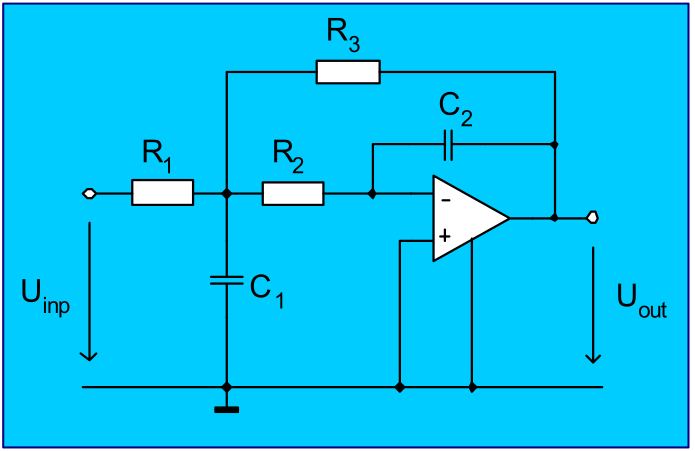
\includegraphics[width=0.7\linewidth]{Obrazky/AE1/MFBDP}
		\caption{ARC Dolná priepusť 2. rádu - Huelsman - MFB, multiple feedback}
		\label{fig:mfbdp}
	\end{subfigure}
	\begin{subfigure}[b]{0.45\textwidth}
		\centering
		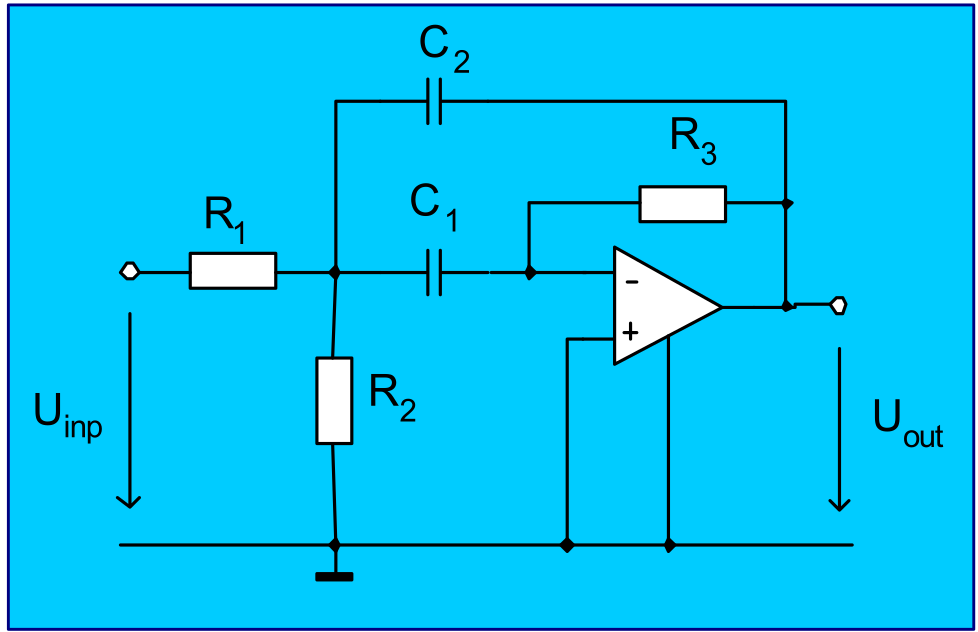
\includegraphics[width=0.7\linewidth]{Obrazky/AE1/MFBPP}
		\caption{ARC pásmová priepusť 2. rádu - Huelsman - MFB, multiple feedback}
		\label{fig:mfbPP}
	\end{subfigure}
	\caption{MFB topológie}
	\label{fig:mfb}
\end{figure}
Parametre \ref{fig:mfb} sa nedajú nezávisle nastavovať.
\begin{equation}
	\begin{aligned}
		K_0 = -\frac{R_3}{R_1} \,, \quad 
		\omega_p = \frac{1}{\sqrt{R_2 R_3 C_1 C_2}} \,, \quad 
		Q_p^{-1} = \sqrt{\frac{C_2}{C_1}} \left( \frac{\sqrt{R_2 R_3}}{R_1} + \sqrt{\frac{R_2}{R_3}} + \sqrt{\frac{R_3}{R_2}} \right) .
	\end{aligned}
\end{equation}
Úpravou MFB topológie \ref{fig:mfbdp} dosiahneme topológiu Sallen-Key, táto topológia má len jednu spätnú väzbu.
\begin{figure}[H]
	\centering
	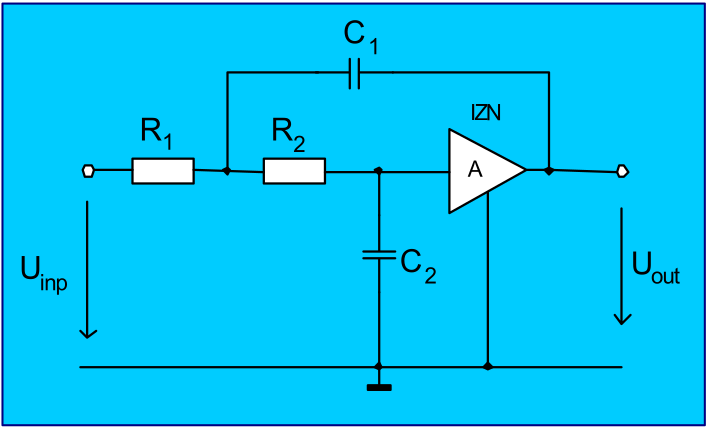
\includegraphics[width=0.4\linewidth]{Obrazky/AE1/sallenKeyDP}
	\caption{ARC 2. rádu dolná priepusť, Sallen-Key}
	\label{fig:sallenkeydp}
\end{figure}
Realizuje sa s neinvertujúcim zosilňovačom. V porovnaní s MFB je jednoduchšia. Obe topológie majú nízke citlivosti na komponenty. Aktívnu priepusť vieme realizovať zámenou R za C. R alebo C sa volia tak aby bolo $R_1 = R_2$ alebo $C_1 = C_2$. Nie však obe naraz.

\section{Aproximačné funkcie filtrov}
Aproximačná, alebo prenosová funkcia, plne popisuje správanie sa filtra v celej frekvenčnej oblasti. Aproximačná funkcia sa volí podľa požadovaného tolerančného kanálu - volí sa tak aby sa modul zmestil do nami definovaného poľa vo frekvenčnej oblasti.
Aproximačných funkcií existuje veľké množstvo, najpoužívanejšie sú uvedené nižšie.
\begin{figure}[H]
	\centering
	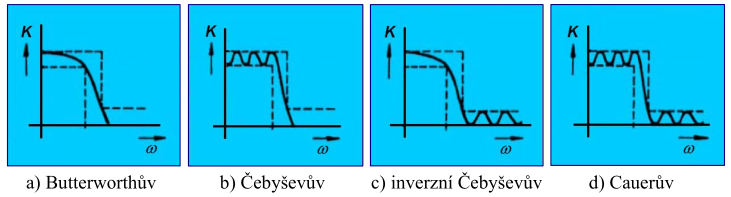
\includegraphics[width=0.7\linewidth]{Obrazky/AE1/aproximacneFunkcie}
	\caption{Bežne používané aproximačné funkcie.}
	\label{fig:aproximacnefunkcie}
\end{figure}
\begin{description}
	\item[Butterworth] Maximálne plochá prenosová charakteristika v priepustnom pásme, no nízka strmosť
	\item[Čebyšev] založené na izotermálnej aproximácií. Majú isté dovolené zvlnenie modulovej charakteristiky či už v priepustnom alebo nepriepustnom pásme (Inverzný Čebyšev)
	\item[Caurer] Dosahujú pri rovnakom ráde najvyššiu strmosť útlmu. Zvlnenie je aj priepustnom aj v nepriepustnom pásme. Nehodia sa pre prenos impulzov.
	\item[Bessel] Pre použitie s konštantným skupinovým oneskorením, majú maximálne lineárnu fázovú charakteristiku. 
\end{description}
\begin{figure}[H]
	\centering
	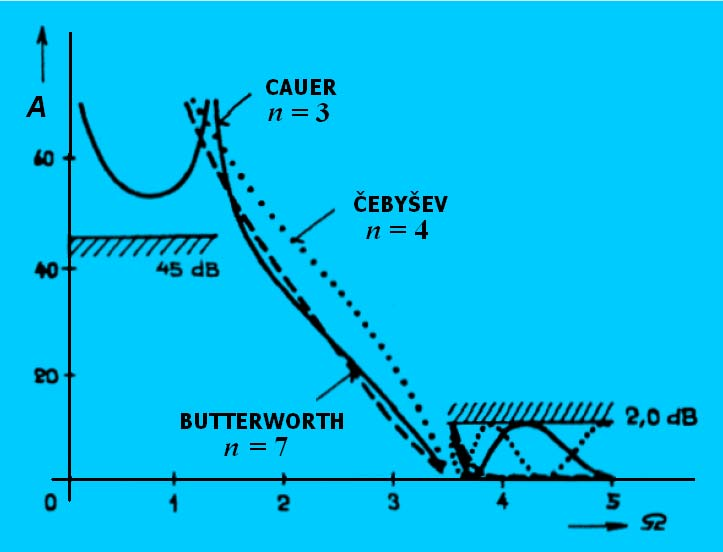
\includegraphics[width=0.4\linewidth]{Obrazky/AE1/porovnanieRadovFiltra}
	\caption{Porovnanie strmosti filtrov podľa rádu $n$}
	\label{fig:porovnanieradovfiltra}
\end{figure}
\section{Filtre vyšších rádov}
Filtre vyšších rádov sa realizujú formou kaskádneho zapojenia filtrov 2. a 1. rádu. V prípade pasívnych filtrov sa najčastejšie realizujú v podobe priečkovej štruktúry s rovnakou impedanciou na vstupe aj na výstupe. Pasívne filtre nie sú vhodné pre realizáciu vyšších rádov z dôvodu veľkosti, komplexnosti a ceny.

Kaskáda znamená súčin niekoľkých dielčich funkcií ktoré dokopy vytvoria funkciu vyššieho rádu. V praxi sa kaskáda navrhuje podľa návrhových tabuliek pre konkrétnu aproximačnú funkciu.

\chapter{Zosilňovače}
%Otázka - Zesilovače: kritéria pro klasifikaci, základní parametry, třídy zesilovačů, účinnost, širokopásmové zesilovače, úzkopásmové (laděné) zesilovače, výkonové (koncové) nf zesilovače. 

Základnou funkciou zosilňovača je zvýšiť užitočný výkon vstupného signálu - zväčší amplitúdu. Pričom by nemal akokoľvek pozmeniť časový priebeh vstupného signálu. Zosilňovače vykazujú stratový výkon. Poznáme jednočinné - ide len do plusu, a dvojčinné zosilňovače.
\section{Kritériá pre klasifikáciu zosilňovačov}
\begin{itemize}
	\item Podľa zosilovanej veličiny
	\begin{itemize}
		\item Zosilňovače napätia - $Z_{in} \rightarrow \text{max}$, $Z_{out} \rightarrow \text{min}$
		\item Zosilňovače prúdu - $Z_{in} \rightarrow \text{min}$, $Z_{out} \rightarrow \text{max}$
		\item Koncové zosilňovače - maximálny výstupný výkon
	\end{itemize}
	\item Podľa záťaže
	\begin{itemize}
		\item Rezistívna - nízkofrekvenčné zos.
		\item Kapacitna
		\item Induktívna - transformátor - koncové zos.
		\item rezonančný obvod - vf, nf zosilňovače
		\item Obezná impedancia
	\end{itemize}
	\item Podľa väzby vstupov
	\begin{itemize}
		\item priama, galvanická väzba - ss zos.
		\item odporová - ss, nf zos.
		\item kapacitná - striedavé zosilňovače
		\item transformátorová - koncové zosilňovače
		\item frekvenčne závislé články - korekčné zosilňovače
	\end{itemize}
	\item Podľa veľkosti vstupného signálu
	\begin{itemize}
		\item malý signál - lineárne zos.
		\item veľký signál - nelineárne zos.
	\end{itemize}
	\item Podľa pracovnej frekvencie
	\begin{itemize}
		\item jednosmerné - ss
		\item striedavé nf - audio
		\item striedavé vg - rádio
	\end{itemize}
	\item Podľa šírky pásma
	\begin{itemize}
		\item úzkopásmové - ladené vf
		\item širokopásmové - nf a vf
	\end{itemize}
	\item Podľa aktívneho prvku
	\begin{itemize}
		\item BJT
		\item FET
		\item Elektrónky
	\end{itemize}
	\item Podľa polohy pracovného bodu
	\begin{itemize}
		\item trieda A
		\item trieda B
		\item trieda AB
		\item trieda C
	\end{itemize}
\end{itemize}
\section{Parametre zosilňovačov}
Obdovodé funkcie \(K_U, \; K_I, \; K_P, \; Z_{inp}, \; Z_{out}\). \newline
Charakteristiky \(K(\omega), \; \varphi(\omega), \; u_{out}(u)_{in}\)
\begin{align}
	\underset{\text{Harmonické skreslenie}}{THD = \sqrt{\frac{U_2^2 + U_3^2 + \dots + U_n^2}{U_1^2 + U_2^2 + \dots + U_n^2}}}
	\qquad \quad 
	\underset{\text{(Gain Bandwidth Product)}}{GBP} = K_0 \cdot B 
	\qquad \quad 
	\underset{\text{Šumové číslo}}{F = \frac{\frac{P_{in}^{S}}{P_{in}^{N}}}{\frac{P_{out}^{S}}{P_{out}^{N}}}}
\end{align}
\section{Triedy zosilňovačov}
Existuje ich veľa, hlavné sú:
\begin{description}
	\item[Trieda A] Účinnosť malá, pod \qty{50}{\%}, používajú sa na malé signály. Minimálne skreslenie.
	\item[Trieda B] Účinnosť rádovo \qty{75}{\%}, dvojčinné zosilňovače, jedna vetva zosilňovača zosiluje kladnú a druhá zápornú pol-vlnu vstupného signálu
	\item[Trieda AB] Účinnosť podobne ako trieda B, dosahujú vyššie skreslenie, neprenášajú celú vlnu. Bežné v audiotechnike.
	\item[Trieda C] Teoretická účinnosť až \qty{100}{\%}. Extrémne miery skreslenia, používajú sa ako VF.
	\item[Trieda D] Jedná sa o digitálny zosilňovač ktorý na výstupe produkuje v podstate PWM. Skladá sa z generátora referenčného priebehu  a komparátora tohto priebehu s vstupným signálom.
\end{description}
\begin{figure}[H]
	\centering
	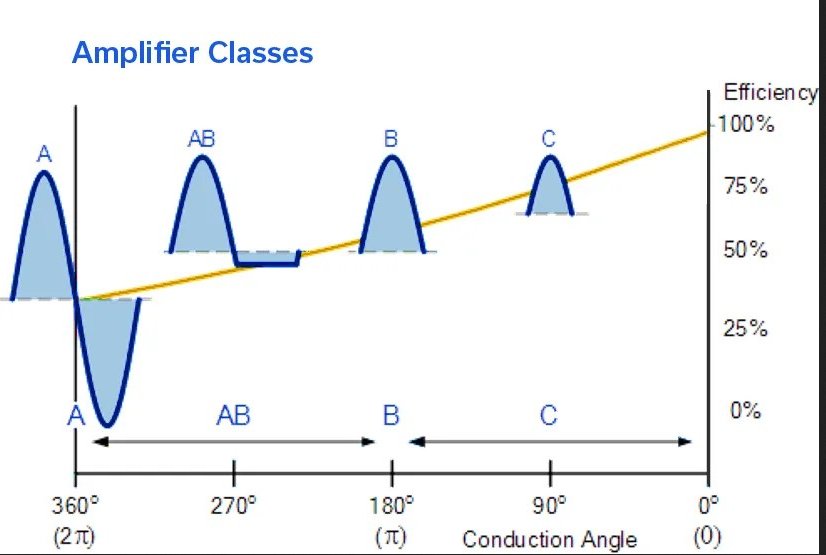
\includegraphics[width=0.4\linewidth]{Obrazky/AE1/TretiaOtazka/ZosilnovaceTriedy}
	\caption{Porovnanie výstupných priebeho základných tried zosilňovačov}
	\label{fig:zosilnovacetriedy}
\end{figure}
Trieda zosilňovača zároveň hovorí aj o jeho pracovnom bode. 
\begin{description}
	\item[Trieda A] Pracovný bod nastavený do stredu lineárnej časti charakteristiky
	\item[Trieda B] Pracovný bod je nastavený do bodu zániku kolektorového prúdu
	\item[Trieda C] Pracovný bod je nastavený hlboko do oblasti zániku kolektorového prúdu
	\item[Trieda AB] Pracovný bod je nastavený medzi stred lineárnej časti a bod zániku kolektorového prúdu
\end{description}
\section{Široko-pásmové zosilňovače}
Rozšíriť pásmo ktoré zosilňovač prenáša je možné výberom zapojenia (SC, SB, SE), využitím spätnej väzby, či modifikáciou zapojenia - delením záťaže.

Frekvenčne nezávislá spätná väzba - zložená z čiste rezistívnych komponentov, sa dá využiť tiež, jej využitie je v plyve zápornej spätnej väzby.
\begin{figure}[H]
	\centering
	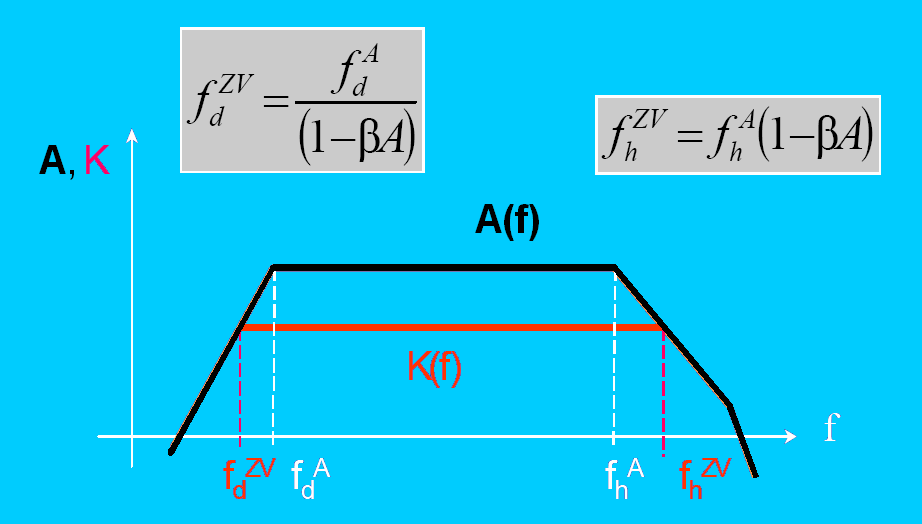
\includegraphics[width=0.4\linewidth]{Obrazky/AE1/TretiaOtazka/zapornaSpatnaVazba}
	\caption{Vplyv zápornej spätnej väzby na šírku pásma - teda medzné frekvencie.}
	\label{fig:zapornaspatnavazba}
\end{figure}

\begin{figure}[H]
	\centering
	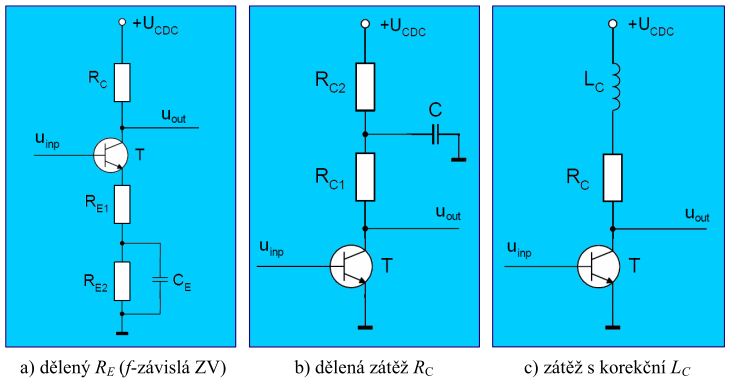
\includegraphics[width=0.7\linewidth]{Obrazky/AE1/TretiaOtazka/frekvenceZavislaVazba}
	\caption{Realizácia korekcie frek. char. formou závislej spätnej väzby}
	\label{fig:frekvencezavislavazba}
\end{figure}
Dá sa využiť aj frekvenčne závislá väzba \ref{fig:frekvencezavislavazba}. \ref{fig:frekvencezavislavazba}a - Kondenzátor $C_E$ sa vo vyšších frekvenciách skratuje, čo bude znamenať menšiu spätnú väzbu vo vyššom pásme. Rovnako to funguje aj pri \ref{fig:frekvencezavislavazba}b. Záťaž s korekčným $L_C$ nám zase poskytne v modulovej charakteristike rezonančné prevýšenie, keďže indukčnosť L tvorí s parazitnou kapacitou výstupu rezonančný obvod.

\section{Úzko-pásmové zosilňovače}
Jedná sa najmä o selektívne zosilňovače, ktoré zosilňujú len isté frekvencie. V malých výkonoch sa na tento účel používa trieda A v lineárnom režime. V závislosti od spôsobu napájania môže vyzerať principiálne zapojenie:
\begin{figure}[H]
	\centering
	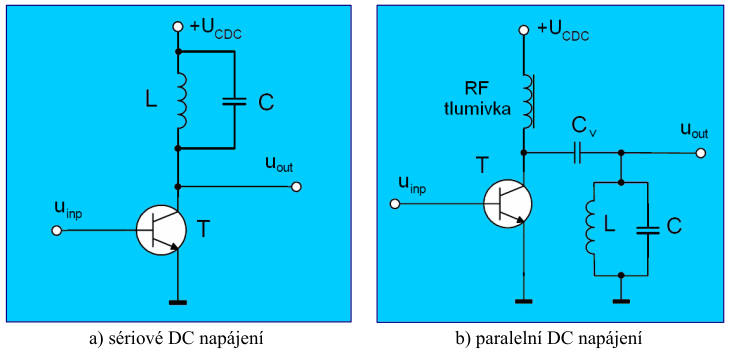
\includegraphics[width=0.6\linewidth]{Obrazky/AE1/TretiaOtazka/selektivnyZosi}
	\caption{Selektívny zosilňovač s jedným ladeným obvodom}
	\label{fig:selektivnyzosi}
\end{figure}
Selektívne zosilňovače mávajú rôzny parameter Q - Veľkosť prekmitu v charakteristike. Ladené obvody sa dajú rôzne pripájať a upravovať. Nakoľko toto nie je výkonový zosilňovač, tak to ešte musíme výkonovo zosilniť triedou C. Tá je pripojená k takémuto zosilňovaču odbočkou vytvorenou z autotransformátora.

VF zosilňovače sú náchylné na nestabilitu ktorá vzniká parazitnými kapacitami v tranzistore, ktoré odtlmia rezonančný obvod. Preto sa robí:
\begin{itemize}
	\item Neutralizácia zos. = opatrenie proti rozkmitaniu
	\item Unilaterizácia zos. = zabránenie spätného prenosu na vstup
\end{itemize}
\subsubsection{Výkonové úzko-pásmové}
Výkonové zosilňovače sa konštruujú z prvkov FET. Konštruujú sa v triede C. Pracujú ako koncové stupne, ktorých úlohou je zabezpečiť maximálny výstupný výkon, pracujú v nelineárnom režime. Pre veľmi veľké výkony sa stále používajú elektrónky.
\subsubsection{S viacerími ladenými obvodmi}
Dôvod využitia viacerých ladených obvodov môže byť zväčšenie šírky pásma. Ladené obvody pripájame na vstup a na výstup. Môžu byť ladené zhodne alebo aj nie.
\begin{figure}[H]
	\centering
	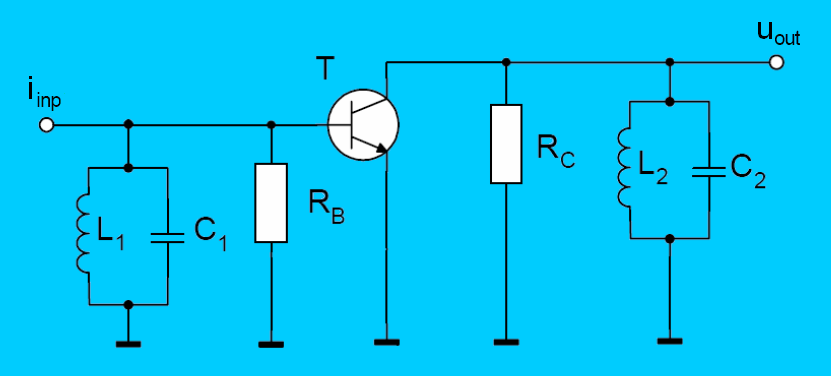
\includegraphics[width=0.4\linewidth]{Obrazky/AE1/TretiaOtazka/ZosikViacObvod1}
	\caption{Zosilňovač s viacerými ladenými obvodmi}
	\label{fig:zosikviacobvod}
\end{figure}

\begin{figure}[H]
	\centering
	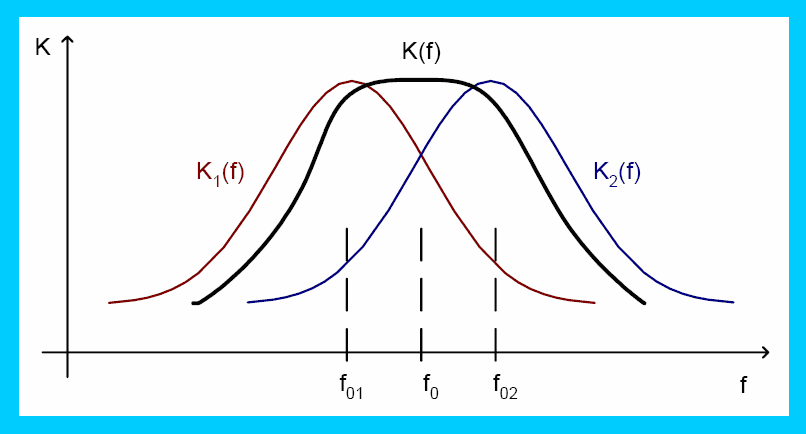
\includegraphics[width=0.4\linewidth]{Obrazky/AE1/TretiaOtazka/frekCharViacObvod}
	\caption{Frekvenčná charakteristika s viacerými ladenými obvodmi}
	\label{fig:frekcharviacobvod}
\end{figure}
Rozšírenie modulovej charakteristiky je možné použitím aj viazaného ladeného obvodu, založeného na indukčnosti - Induktívna väzba.
\section{Výkonové NF zosilňovače}
Výkonové zosilňovače sa realizujú v triedach A, B či AB. Majú poskytnúť maximálny akustický výkon, pričom sa hľadá optimálna záťaž pre maximálny výkon. Rozdelujú sa:
\begin{itemize}
	\item Podľa typu zapojenia
	\begin{itemize}
		\item SE
		\item SC
		\item Jednočinné / dvojčinné
	\end{itemize}
	\item Väzba medzi stupňami a záťažou
	\begin{itemize}
		\item Priama
		\item Kapacitná
		\item Transformátorová
	\end{itemize}
	\item Trieda
	\begin{itemize}
		\item Základné: A, B, AB, C
		\item Spínané: D, E, S, T, F, G, H
	\end{itemize}
\end{itemize}
Zosilňovač jednočinný v triede A s rezistívnou záťažou - používa sa minimálne, má účinnosť len  $25 \%$, no minimálne skreslenie. Pokiaľ nahradíme odpor $R_C$ transformátorom, dosiahneme účinnosti $50 \%$

Zosilňovač triedy B s transformátorom - obsahuje vstupný a výstupný transformátor. Teoretická hodnota účinnosti je $78.5\%$. Budiaci signál sa privádza fázovo posunutý na T1 a T2. 

Zosilňovač triedy B bez transformátora - nemá transformátor ani na vstupe ani na výstupe. 
\begin{figure}[H]
	\centering
	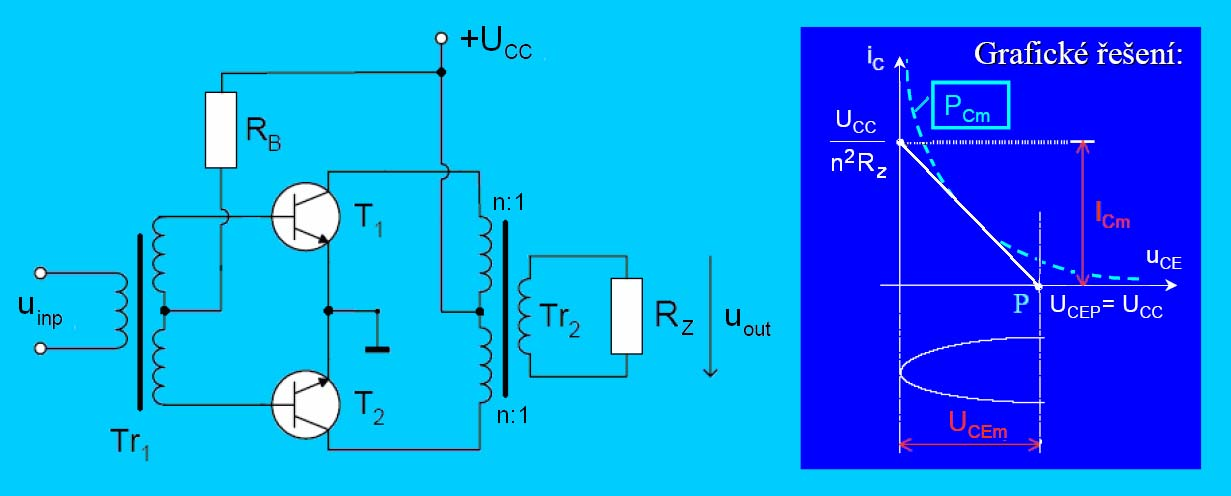
\includegraphics[width=0.7\linewidth]{Obrazky/AE1/TretiaOtazka/triedaBtransformator}
	\caption{NF zosilňovač triedy B s transformátormi}
	\label{fig:triedabtransformator}
\end{figure}
Zosilňovač triedy B bez transformátorov využíva fázový invertor miesto vstupného transformátora.
\begin{figure}[H]
	\centering
	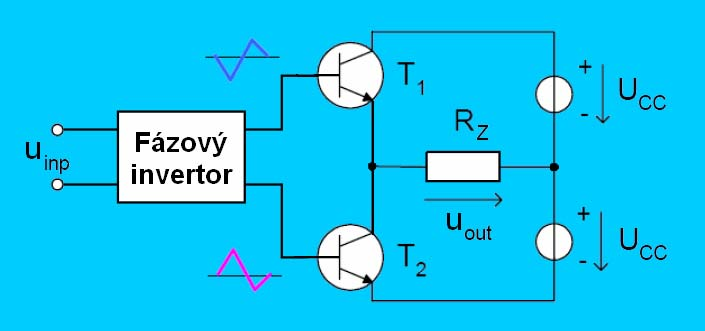
\includegraphics[width=0.7\linewidth]{Obrazky/AE1/TretiaOtazka/BbezTrafa}
	\caption{Zosilňovač triedy B bez transformátora.}
	\label{fig:bbeztrafa}
\end{figure}
\begin{figure}[H]
	\centering
	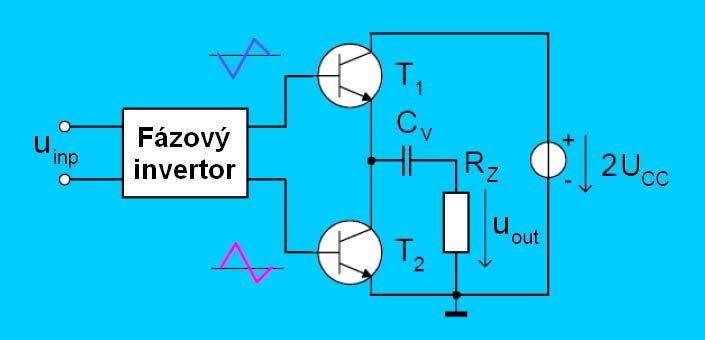
\includegraphics[width=0.7\linewidth]{Obrazky/AE1/TretiaOtazka/BbezTrafaDC}
	\caption{Zosilňovač triedy B s nesymetrickým zdrojom..}
	\label{fig:bbeztrafadc}
\end{figure}

V prípade, že sa použije nesymetrický DC zdroj, je potrebný väzobný kondenzátor na výstupe.

Dajú sa použiť aj komplementárne tranzistory, toto zjednoduší vstupnú budiacu časť. Používajú sa BJT tranzistory v pároch PNP a NPN.
\begin{figure}[H]
	\centering
	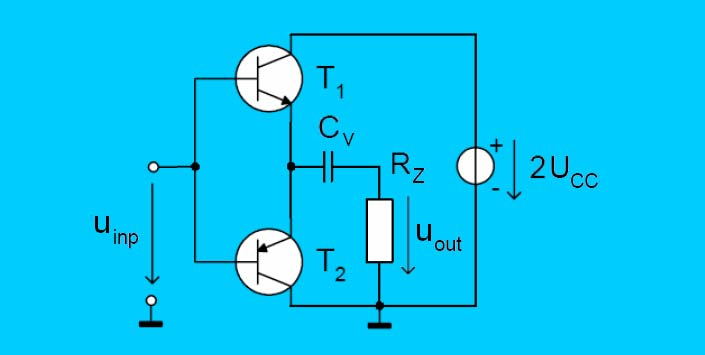
\includegraphics[width=0.7\linewidth]{Obrazky/AE1/TretiaOtazka/PNPNPNzosik}
	\caption{Zosilňovač triedy B s komplementárnym PNP NPN párom}
	\label{fig:pnpnpnzosik}
\end{figure}
Komplementárty pár musí mať rovnaké vlastnosti. Inak dochádza k skresleniu v oblasti prechodu nulou. Na potlačenie skreslenia sa používa napríklad trieda AB, resp. nastavenie kľudového pracovného bodu.

\begin{figure}[H]
	\centering
	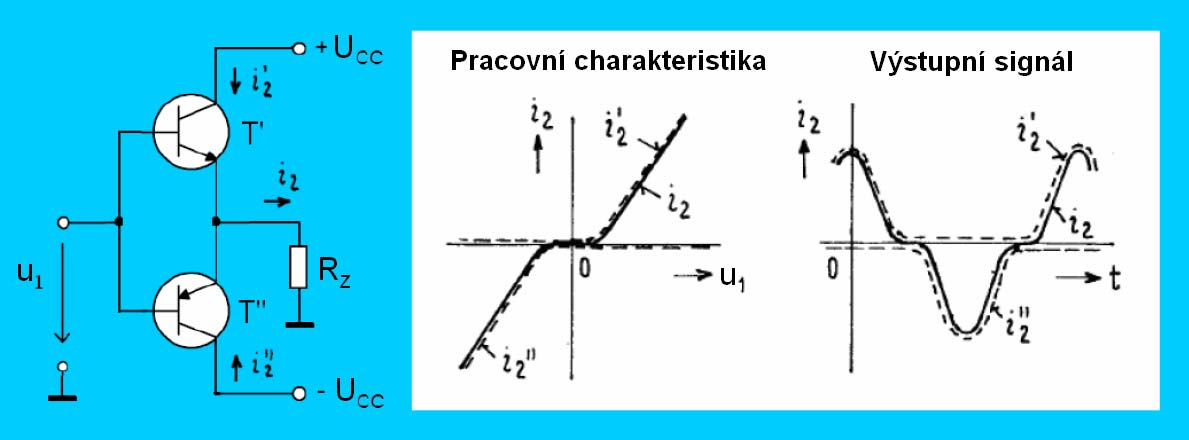
\includegraphics[width=0.7\linewidth]{Obrazky/AE1/TretiaOtazka/zkrelsenieB}
	\caption{Zkreslenie v komplementárnom zosilňovači triedy B}
	\label{fig:zkrelsenieb}
\end{figure}
\begin{figure}[H]
	\centering
	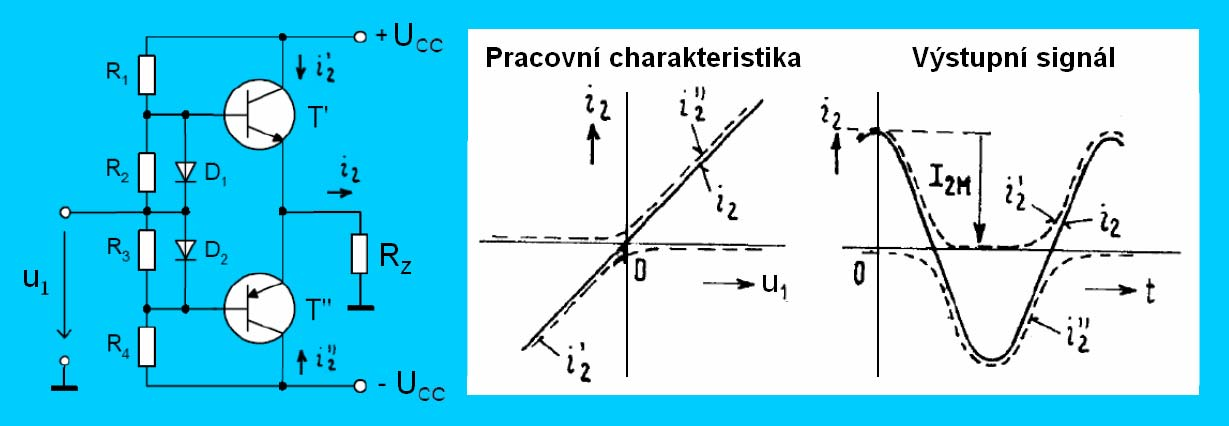
\includegraphics[width=0.7\linewidth]{Obrazky/AE1/TretiaOtazka/skreslenieAB}
	\caption{Trieda AB s komplementárnymi tranzistormi.}
	\label{fig:skreslenieab}
\end{figure}
\subsubsection{Spínané zosilňovače}
Spínaný zosilňovač sa realizuje s unipolárnymi tranzistormi. V podstate sa jedná o PWM generátor pripojený k výkonovému mostíku. Na výstup sa musí pripojiť LC filter.
\begin{figure}[H]
	\centering
	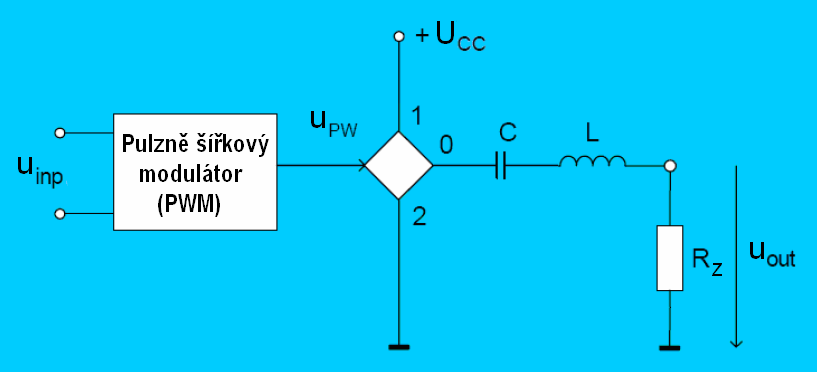
\includegraphics[width=0.7\linewidth]{Obrazky/AE1/TretiaOtazka/spinanyZosik}
	\caption{Spínaný zosilňovač}
	\label{fig:spinanyzosik}
\end{figure}



	% !TeX root = statnicaEKT.tex
% !TeX spellcheck = sk_SK-Slovak
\part{BPC-AE2 - Analógová elektronika 2}
%\chapter{BPC-AE2 - Analógová elektronika 2}
\begin{huge}
Otázky:
\newline
\end{huge}
\begin{enumerate}
\item Otázka - Lineární a linearizované obvody: návrh jednostupňových zesilovačů s FET; oscilátory - charakteristická rovnice, oscilační podmínka, ladění, stabilizace amplitudy; aktivní součástky - konvejory, řízené zesilovače, násobičky, transkonduktor.
\item Otázka - Spínací a tvarovací obvody: přechodné děje a přenos signálu lineární a nelineární soustavou - přenosové články, kaskáda, zpoždění, doba hrany, kompenzovaný dělič; diodové funkční měniče; tranzistorové spínače - typy, ztráty, zátěže; klopné obvody, realizace; komparátory - prahové úrovně, hystereze, realizace; generátory průběhů.
\item Otázka Operační zesilovače (vlastnosti a použití): konstrukce – diferenční pár, Millerův OZ; provoz OZ - kompenzace a korekce kmitočtové charakteristiky, nesymetrie, rychlost přeběhu, šum, napájení, ESD, ochrany.

\end{enumerate}
\newpage
\chapter{Lineárne a linearizované obvody}
\subsection{Linearizácia pri tranzistoroch}
\textit{Len pre info} - Linearizáciou sa rozumie obmedzenie alebo odstránenie nelineárnej závislosti výstupného prúdu či napätia na vstupnej veličine. Väčšinou toto robíme s použitím degradačného rezistora, ktorý berie väčšiu časť premeny napätia na prúd na seba. Pri použití degradačného rezistora však klesá maximálna dosiahnuteľná hodnota $g_m$ s rastúcim degradačným odporom, rovnako sa prejavuje šum a výrobný rozptyl súčiastiek. 
\begin{figure}[H]
\centering
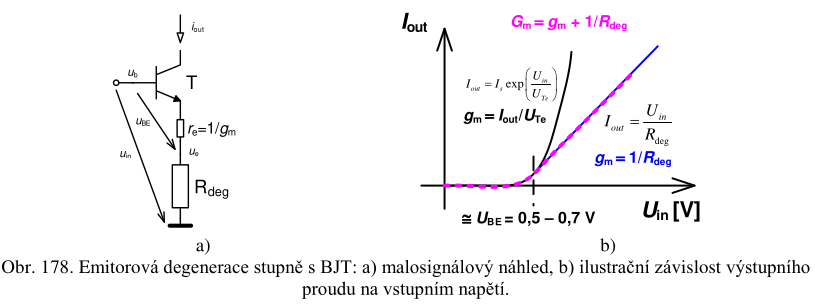
\includegraphics[width=0.7\linewidth]{Obrazky/AE2/1Otazka/linearizaciaBJT}
\caption{Závislosť výstupného prúdu na vstupnom napätí BJT}
\label{fig:linearizaciabjt}
\end{figure}
\begin{figure}[H]
\centering
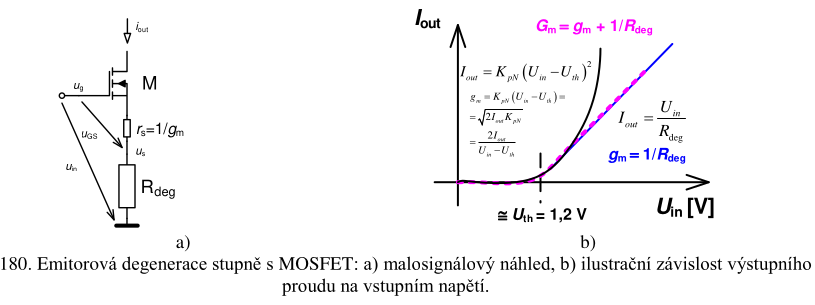
\includegraphics[width=0.7\linewidth]{Obrazky/AE2/1Otazka/linearizaciaMOSFET}
\caption{Závislosť výstupného prúdu na vstupnom napätí MOSFET}
\label{fig:linearizaciamosfet}
\end{figure}
\section{Základné parametre pre JFET a MOSFET}
\subsection{JFET}
\begin{itemize}
\item Kanál existuje aj bez $U_{GS}$ napätia
\item Pracuje v ochudzovacom režime $\rightarrow$ s $U_{GS}$ sa kanál zmenšuje $\rightarrow$ pri $U_{GS_{OFF}}$ kanál zaniká
\item maximálny prúd $I_{DSS}$ je pri nepripojenom napätí $U_{GS}$
\item \textbf{Výhody JFET}
\begin{itemize}
	\item Vysoký vstupný odpor
	\item Menší vplyv šumu
	\item Vysoký výkonový zisk
	\item Negatívny teplotný koeficient odporu $\rightarrow$ s rastúcou teplotou klesá odpor kanálu
\end{itemize}
\item \textbf{Nevýhody JFET}
\begin{itemize}
	\item Silne nelineárny
	\item Vysoké tolerancie parametrov $\rightarrow$ ťažký návrh pre niektoré aplikácie
\end{itemize}
\end{itemize}
\subsection{MOSFET}
\begin{itemize}
\item Kanál bez priloženého napätia $U_{GS}$ neexistuje
\item Pracuje v obohacovacom režime $\rightarrow$ s rastúcim $U_{GS}$ $\rightarrow$ sa kanál zväčšuje
\item Režimy v ktorých pracuje MOSFET
\begin{itemize}
	\item \textbf{Podprahový režim - slabá inverzia}
		\subitem $U_{GS} < U_{TH}$
		\subitem Správanie ako BJT tranzistor $\rightarrow$ $I_D$ závisí na $U_{GS}$ exponencionálne
		\subitem Na piču frekvenčné vlastnosti
		\subitem Maximálna hodnota $I_D$ je rovnako na piču malá
		\subitem Veľké tolerancie a teplotný rozptyl parametrov
		\subitem Závislosť $I_D$ na $U_{GS}$ je exponenciálna: \underline{\(I_D = konst. \cdot \exp\left[\frac{U_{GS}}{n \cdot U_{Te}}\right]\)}
	\item  \textbf{Lineárny režim - odpor/trióda}
		\subitem $0 < U_{DS} < (U_{GS} - U_{TH}) = U_{DS_{SAT}}; \; U_{GS} > U_{TH}$
		\subitem Saturačné napätie $U_{DS_{SAT}}$ predstavuje hranicu medzi odporovým režimom a režimom silnej inverzie
		\subitem MOSFET pracuje ako napätím riadený odpor, vníma sa v určitých medziach lineárne
	\item \textbf{Režim silnej inverzie - saturačný režim}
		\subitem \underline{Najčastejšie používaný režim}
		\subitem Správa sa ako zdroj prúdu
		\subitem $U_{DS} > U_{DS_{SAT}} = (U_{GS} - U_{TH}) ; \; U_{GS} > U_{TH}$
		\subitem Závislosť $I_D$ na $U_{GS}$ kvadratická: \underline{\(I_D = K_P \cdot\left(U_{GS} - U_{TH}\right)^2\)}
		\subitem Veľkosť $U_{DS}$ má vplyv na rovnomernosť rozloženie nosičov náboja, s rastúcim $U_{DS}$, stúpa teda aj $I_D$, \underline{nie však ideálne} $\rightarrow$ spôsobené konečným odporom kanálu $\rightarrow$ vyjadruje sa veľkosťou koeficientu modulácie dĺžky kanálu $\lambda$, ktorý spôsobuje náklon kriviek v saturačnej oblasti, samotná $\lambda$ závisí na dĺžke kanálu \emph{L}.
		\subitem $I_D$ je možné riadiť aj \emph{BULKom} - samostatnou svorkou na tranzistore $\rightarrow$ môže to spôsobiť problémy so stabilitou $\rightarrow$ pripája sa na \emph{SOURCE}.
	\item  \textbf{Režim rýchlostnej saturácie nosičov náboja}
		\subitem \(U_{DS} >> U_{DS_{SAT}}; \; U_{GS} > U_{TH}\)
		\subitem $U_{GS}$ už nemá vplyv na transkonduktanciu $g_m$ $\rightarrow$ nedá sa riadiť $\rightarrow$ veľké hodnoty $I_D$.
		\subitem Dochádza k degradácií maximálnej rýchlosti nosičov.
\end{itemize}
\end{itemize}
\begin{figure}[H]
	\centering
	\begin{subfigure}[b]{0.48\textwidth}
		\centering
		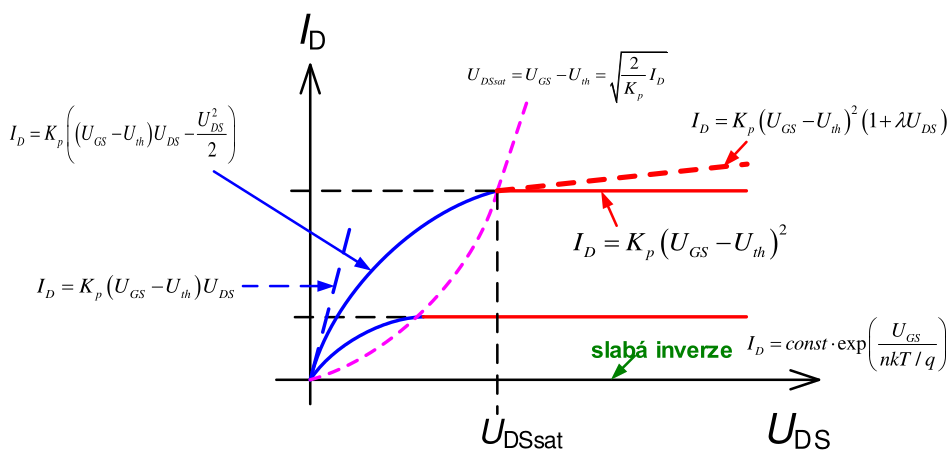
\includegraphics[width=\linewidth]{Obrazky/AE2/1Otazka/IDvsUDSMOSFET}
		\caption{Závisloť $I_D$ na $U_{DS}$}
		\label{fig:idvsudsmosfet}
	\end{subfigure}
	\begin{subfigure}[b]{0.48\textwidth}
		\centering
		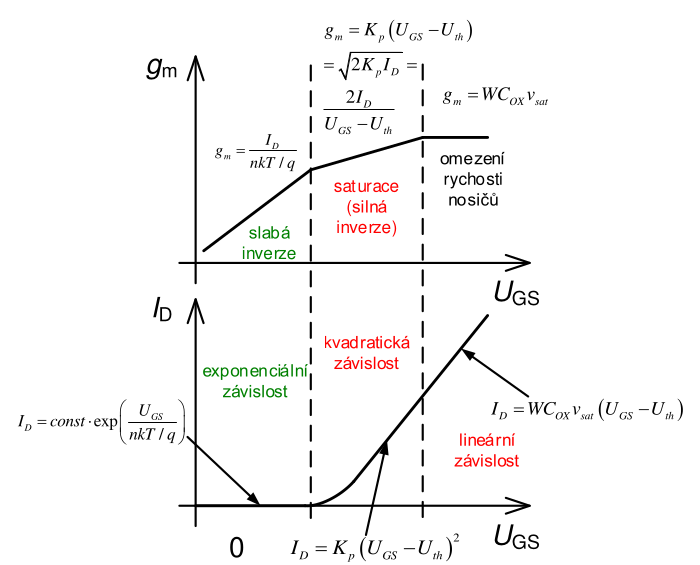
\includegraphics[width=\linewidth]{Obrazky/AE2/1Otazka/IDvsUGSMOSFET}
		\caption{Závislosť $g_m$ a $I_D$ na $U_{GS}$}
		\label{fig:idvsugsmosfet}
	\end{subfigure}
	\label{fig:prevadzkoveRezimyMosfet}
	\caption{Zhrnutie prevádzkových režimov pre MOSFET s indukovaným kanálom}
\end{figure}
\begin{figure}[H]
	\centering
	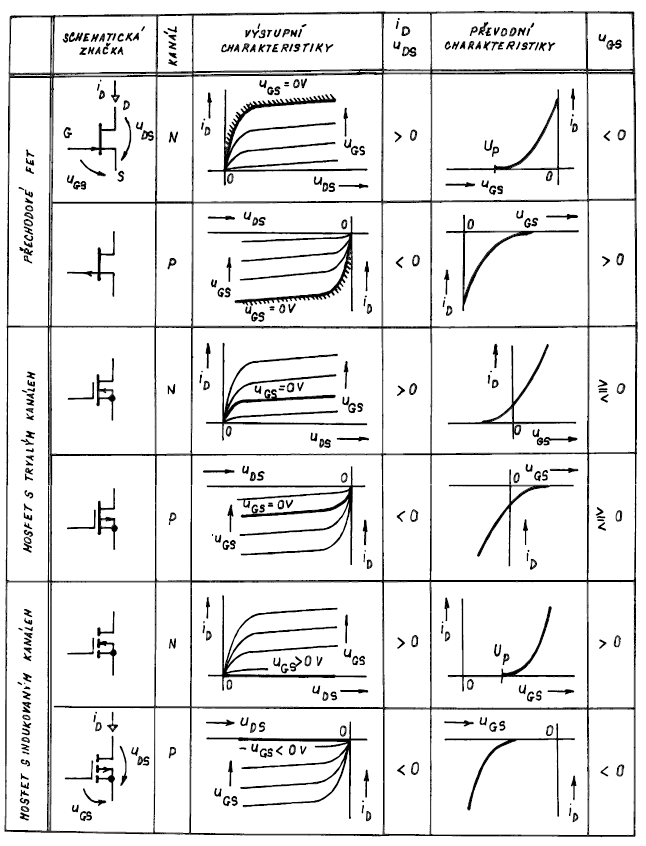
\includegraphics[width=\linewidth]{Obrazky/AE2/1Otazka/PrehladSpravaniaUnipolarov}
	\caption{Prehľad typov a správania sa rôznych unipolárnych tranzistorov}
	\label{fig:prehladspravaniaunipolarov}
\end{figure}
\newpage
\section{Návrh N-JFET zosilňovača}
\begin{figure}[H]
	
	\begin{subfigure}[b]{0.48\textwidth}
	\centering
	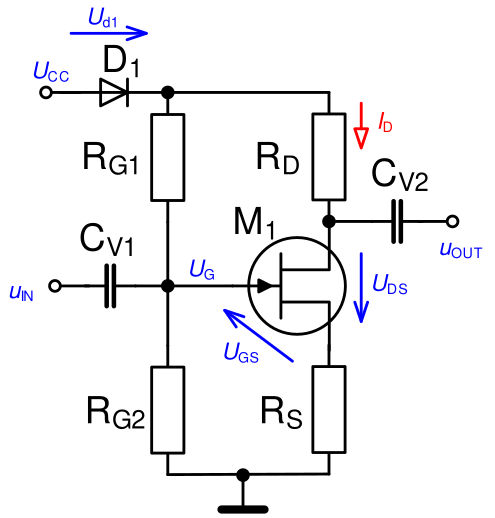
\includegraphics[width=0.7\linewidth]{Obrazky/AE2/1Otazka/NJFET-zapojenie}
	\caption{Funkčné zapojenie N-JFET zosilňovača}
	\label{fig:njfet-zapojenie}
	\end{subfigure}
	\begin{subfigure}[b]{0.48\textwidth}
	\centering
	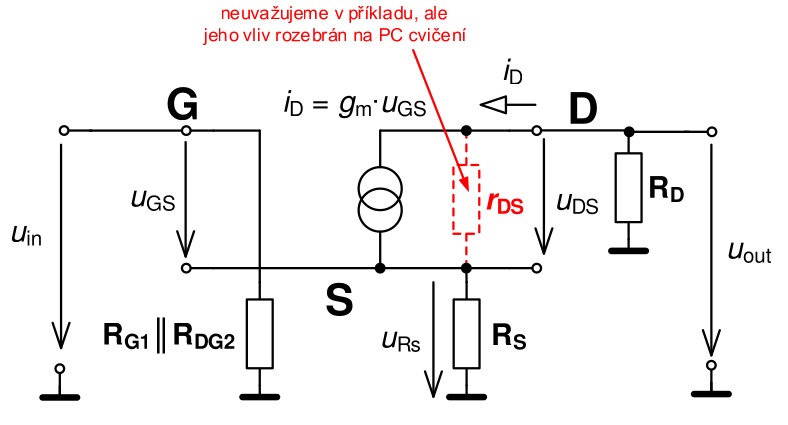
\includegraphics[width=0.7\linewidth]{Obrazky/AE2/1Otazka/NJFET-zapojenie-malosignalModel}
	\caption{Malosignálový model N-JFET zosilňovača}
	\label{fig:njfet-zapojenie-malosignalmodel}
	\end{subfigure}
\end{figure}
Približný postup návrhu:
\begin{enumerate}
	\item Potrebné zvoliť zosilnenie $K_U$ čo chceme dosiahnuť, $U_{DS}$ a $U_{GS}$ sa zvolia tak aby ležali v stredoch charakteristík pre $U_{DS}$ a $U_{GS}$.
	\item Na základe pracovného bodu sa zistia hodnoty $I_{DSS}$ a $U_{GS_{OFF}}$.
	\item Vyráta sa $I_D$, ktoré definuje kľudový pracovný bod.
	\item Zvolí sa vhodný pomer $\frac{R_D}{R_S}$.
	\item Vypočíta sa $g_m$ v pracovnom bode.
	\item Určenie hodnôt $R_S$ a $R_D$.
	\item Výpočet napätia $U_{G}$ v strede deliča.
	\item Na základe výpočtu napätia v deliči zvoliť $R_{G1}$ a dopočítať $R_{G2}$. 
	\item Výpočet väzobných kapacít $C_V$ podľa požadovanej dolnej medznej frekvencie - horná je daná JFET kapacitami - dané pomerom deliča $R_{G1}$ a $R_{G2}$ - počíta sa klasicky ako CR článok.
	\subitem Pokiaľ je známa hodnota záťaže na výstupe $R_L$, je treba ju zahrnúť a podľa nej spočítať vhodné $C_{V2}$ - uvažuje sa ako $R_D + R_L$.
	\item Pokiaľ chceme poznať výstupný rozkmit napätia musím uvažovať veľkosignálové správanie $U_{OUT}$ - ale nie je to lineárne ten výstup.
\end{enumerate}
\section{Návrh MOSFET zosilňovača}
Principiálna schéma zapojenia je rovnaká ako na \ref{fig:njfet-zapojenie}.
Narozdiel od JFET zosilňovača pri ktorom volíme pracovný bod v strede prevodových charakteristík, MOSFET musí byť v saturačnom režime na to aby fungoval ako zosilňovač.
Približný proces návrhu:
\begin{enumerate}
	\item Špecifikácia parametrov ako $I_D$, $K_U$ a podobne
	\item Určenie DC pracovného bodu do stredu oblasti saturačného režimu - sme cca v lineárnej oblasti
	\subitem Spočítať/zvoliť $I_D$
	\subitem Spočítať vstupný delič $R_{G1}$ a $R_{G2}$, $\rightarrow$ netečie tam žiaden prúd, obyčajný pomer teda
	\subitem Na základe pomeru vstupného deliča určite napätie $U_G$
	\subitem \underline{V podstate sa na základe veľko signálovej analýzy spočíta pokojový operačný bod DC}
	\item Na základe DC bodu vieme určiť transkonduktanciu skrz malosignálový model
\end{enumerate}
Keby som nevedel nič iné tak by som to zhrnul asi tak, že dôležitý je DC bod aj pri JFET a aj pri MOSFET zosilňovači.

\section{Oscilátory}
Oscilátor - Harmonický oscilátor je lienárny či linearizovaný obvod ktorý produkuje spektrálne čisté harmonické signály odvodené od funkcií sinus či cosinus. Na svoju činnosť potrebujú vždy aktívny element - tranzistor / operák / elektronku.
Podľa typu kmitajúceho okruhu delíme na:
\begin{itemize}
\item RC oscilátory - pásmo do 1MHz
\item LC oscilátory - pásmo od desiatok kHz až po stovky MHz
\begin{itemize}
	\item Dvojbodové
	\subitem Bežný Paralelný LC rezonančný obvod s paralelným záporným dynamickým odporom realizovaným tunelovou diódou - ten odtlmuje LC obvod - nahradzuje jeho straty
	\item Trojbodové 
	\subitem Colpitts
	\subitem Hartley
\end{itemize}
\item Kryštalické - jednotky až stovky MHz
\end{itemize}
RC a LC oscilátory sa dajú zjednodiť aj do skupiny \underline{Spätnoväzobných oscilátorov}.

\subsection{Popis princípu oscilátora}
Oscilátor využíva kladnú spätnú väzbu ktorá na vstup aktívneho prvku prináša výstupný signál s rovnakou fázou. Spätná väzba musí byť frekvenčne selektívna, nezáleží až tak na amplitúdovej charakteristike ale na fázovej, kmity vznikajú práve vďaka zosilneniu na aktívnom prvku. Zároveň aktívny prvok musí mať dostatočné zosilnenie na to, aby pokryl straty v pasívnej časti - spätnej väzbe. Oscilátor musí obsahovať aj obvod pre tlmenie kmitov - riadenie amplitúdy. Realizuje sa to zápornou spätnou väzbou. Riadenie amplitúdy je dôležité, aby nedošlo k saturácií výstupu. Oscilátor nepotrebuje budenie, dôsledkom zosilnenia aktívneho prvku sa vybudí sám. Pre funkciu oscilátora platia dve podmienky: Amplitúdová - hovorí o množstve energie ktorú musí dodať aktívny prvok na to aby sa pokryli straty v pasívnom obvode. Fázová - hovorí, že posuv fáze selektívnym obvodom a zosilňovačom musí byť nulový - resp násobky pi.


\begin{figure}[H]
\centering
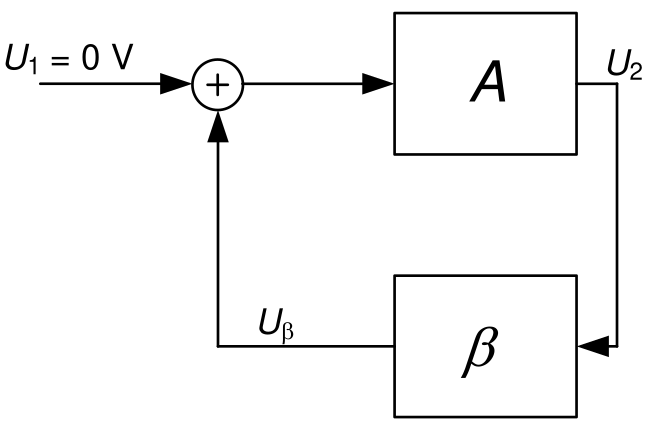
\includegraphics[width=0.35\linewidth]{Obrazky/AE2/1Otazka/principZVoscilatora}
\caption{Princíp spätnoväzobného oscilátora}
\label{fig:principzvoscilatora}
\end{figure}
\section{Oscilačné podmienky}
\begin{itemize}
\item Obvod musí byť na medzi stability
\item Korene charakteristickej rovnice musia ležať presne na Imaginárnej ose a byť komplexne združené
\item Pre prenos ZV platí Blackov vzťah: 

\begin{equation}
	K(s) = \frac{U_2}{U_1} = \frac{A}{1 \pm \beta(s)A}
\end{equation}

(Pre zápornú ZV platí, že v menovateli je +)

\item Amplitúdová podmienka: 
\begin{equation}
	\beta A = 1
\end{equation}
\item Fázová podmienka:
\begin{equation}
	\varphi_A + \varphi_\beta = 2k\pi
\end{equation}
\end{itemize}
\section{Stabilizácia amplitúdy}
Využíva sa regulačná slučka ktorá reguluje zosilnenie aktívneho prvku.
Systém Regulácie môže byť:
\begin{itemize}
\item Zotrvačný systém stabilizácie:
\begin{itemize}
	\item Zapojený zotrvačný prvok - kondenzátor C - oneskorená reakcia
	\item Funguje len na konkrétnej frekvencii
	\item Fluktuácie - časová nestabilita, fázový šum
	\item Spektrálne čistejšie - menej aktívnych prvkov
\end{itemize}
\item Nelineárny systém stabilizácie:
\begin{itemize}
	\item Vyžíva nelinearity, ktoré pre väčšie amplitúdy znížia zosilnenie (dióda)
	\item Rýchly systém
	\item Nakoľko sú tam aktívne prvky tak to má vyšší šum
\end{itemize}
\end{itemize}
\section{Charakteristická rovnica}
Získava sa pomocou riešenia obvodov cez metódy MUN, MSP. Alebo program SNAP - tam treba dať vstupný a výstupný indikátor - dáme to do miesta vysokej impedancie - v oscilátoroch tam kde je pripojený kondenzátor. V SNAPe nás zaujíma determinant admitančnej matice.

V prípade, že sme schopní identifikovať prenosy A a $\beta$ pomocou Blackovho vzťahu, potom vieme získať charakteristickú rovnicu tak, že obvod:
\begin{enumerate}
\item rozpojíme v mieste delenia $\rightarrow$ zosilňovač - spätná väzba
\item urobíme čoro-moro pri dosadzovaní do:
\begin{equation}
	1 - A\beta = 0
\end{equation}
\end{enumerate}
\section{Ladenie oscilátorov}
Oscilátor vieme ladiť zmenou hodnôt pasívnych prvkov. Ladenie je možné aj elektronicky, pri využití napríklad zosilňovača OTA, kedy zmenou transkonduktancie $g_m$ zmeníme aj frekvenciu oscilátora.
\section{Konvejory - CCII - Diamantový tranzistor}
Niekedy býva sa označuje aj ako OTA, Transkonduktor, Makrotranzistor. Jedná sa však o moderný mnohobran - principiálne prúdový Konvejor 2 generácie.


\begin{figure}[H]
\begin{subfigure}[b]{0.48\textwidth}
	\centering
	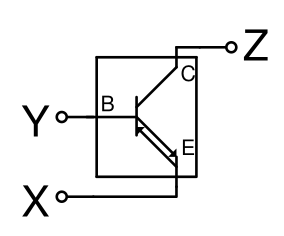
\includegraphics[width=0.5\linewidth]{Obrazky/AE2/1Otazka/diamantovyTranzistor}
	\caption{Ekvivalentné označenie brán konvejoru 2. generácie}
	\label{fig:diamantovytranzistor}
\end{subfigure}
\begin{subfigure}[b]{0.48\textwidth}
	\centering
	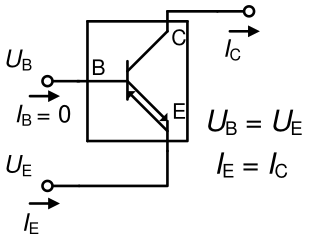
\includegraphics[width=0.5\linewidth]{Obrazky/AE2/1Otazka/PrincipKonvejora}
	\caption{Princíp Konvejora 2. generácie}
	\label{fig:principkonvejora}
\end{subfigure}
\end{figure}
\underline{Konvejorovanie: Sledovanie U a I na vstupoch, prípadne s inverziou.}

Základné vlastnosti konvejorov:
\begin{multicols}{2}
\begin{itemize}
	\item Veľká šírka pásma a rýchlosť prebehu
	\item Možnosť lineárneho nastavovania zisku prúdu medzi X a Z bránami
	\item $Z_{INP}$:
	\begin{itemize}
		\item Vstup X - vysoká impedancia
		\item Vstupy Y a Z - nízka impedancia
	\end{itemize}
	\item Horšia linearita, lepšia však ako iné OTA
	\item Nevyžadujú DC biassing
	\item Vo vnútri má zložitú štruktúru - nie je ani PNP ani NPN, z vonku je to precízny~tranzistor
	\item Nastavenie transkonduktancie pomocou degradačného rezistora v emitore $R_E$
\end{itemize}
\end{multicols}
Možné použitia:
\begin{multicols}{2}
\begin{itemize}
	\item Uzemnená báza, Vstup v emitore (svorka X), Výstup v kolektore (svorka Z) $\rightarrow$ dve zapojené takto za sebou $\rightarrow$ Sledovač prúdu
	\item Alebo v časti navrhovaného obvodu
\end{itemize}
\end{multicols}
\section{Násobičky}
\subsection{Prúdovo - napäťová násobička}
Dneska sa už nevyrába. Konkrétne napr. EL2082. Princíp tohto prvku sa však stále používa najmä vo VCA. 

Princíp činnosti: Obvod riadi prúdové zosilnenie, parameter $B_G$, pomocou riadiaceho napätia $U_G$. Dochádza k násobeniu prúdu na vstupe $X$ napätím parametrom $B_G$. Násobenie prebieha v dvoch kvadrantoch prevodovej charakteristiky. Výsledná charakteristika je lineárna a prvok je stabilný.
\begin{figure}[H]
\centering
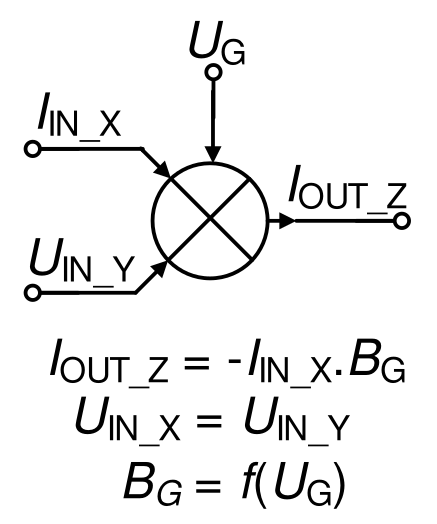
\includegraphics[width=0.15\linewidth]{Obrazky/AE2/1Otazka/principNasobickyPrudNapatie}
\caption{Princíp prúdovo - napäťovej násobičky.}
\label{fig:principnasobickyprudnapatie}
\end{figure}
\subsection{Prúdová násobička}
Podobný princíp ako Prúdovo - Napäťová násobička. Násobí výhradne vstupné prúdy. Násobenie sa deje v štyroch kvadrantoch. Napríklad prvok EL4083. Prúdový vstup $I_Z$ slúži na Biasing.
\begin{figure}[H]
\centering
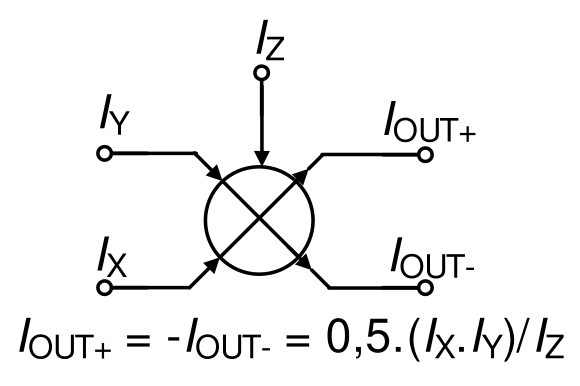
\includegraphics[width=0.35\linewidth]{Obrazky/AE2/1Otazka/prudovaNasobicka}
\caption{Symbol a princíp prúdovej násobičky}
\label{fig:prudovanasobicka}
\end{figure}
\subsection{Napäťové násobičky}
Pracuje s vstupným aj výstupným napätím (asi po zavedení spätnej väzby), násobenie prebieha v štyroch kvadrantoch. V praktických realizáciách sú vstupy plne diferenciálne, pričom je možné pripočítať vstupné napätie k výsledku násobenia. Poskytujú veľké šírky pásma. Používajú sa pre VCA, pre riadené lineárne aj nelineárne štruktúry - amplitúdové modulátory, demodulátory, obvody AGC. Prvok AD835.
\begin{figure}[H]
\centering
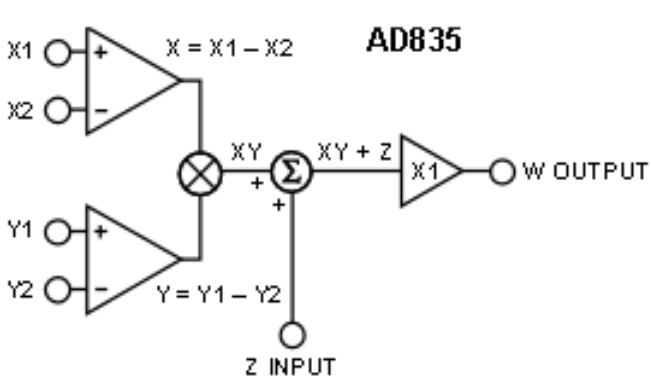
\includegraphics[width=0.35\linewidth]{Obrazky/AE2/1Otazka/napatovaNasobicka}
\caption{Napäťová násobička AD835}
\label{fig:napatovanasobicka}
\end{figure}
\section{Riadené zosilňovače}
VCA - Voltage Controlled Amplifier - možnosť riadenia zisku zosilňovača. Existuje možnosť exponenciálneho (VCA810) a aj lineárneho (VCA822) riadenia zisku.
\section{Transkonduktory - OTA}
Jedná sa o VCCS prvok. Ktorý prevádza vstupné diferenciálne napätie na výstupný prúd. Obsahuje vstupný diferenciálny zosilňovač. Rovnako ako pri iných prvkoch, aj tento je vytlačovaný a ťažko dostupný. Existujú LM13700 a LT1228. Pri ich použití je veľkým problémom veľkosť diferenciálneho vstupného napätia - dochádza k skresleniu výstupného signálu vplyvom vysokej nelinearity parametra $g_m$. Z tohoto dôvodu sa uplatňujú vstupné deliče s vysokým pomerom, bohužiaľ tieto zhoršujú šumové parametre. Nastavenie parametra $g_m$ sa robí riadiacim prúdom - to nie je práve vhodné. Problémom sú aj vstupné odpory, ktoré bývajú závislé od $g_m$ a sú celkom nízke. V púzdrach sa pridávajú aj výstupné buffre.

Parameter $g_m$ sa vytvára s pomocou biasového prúdového zrkadla.
\begin{figure}[H]
\centering
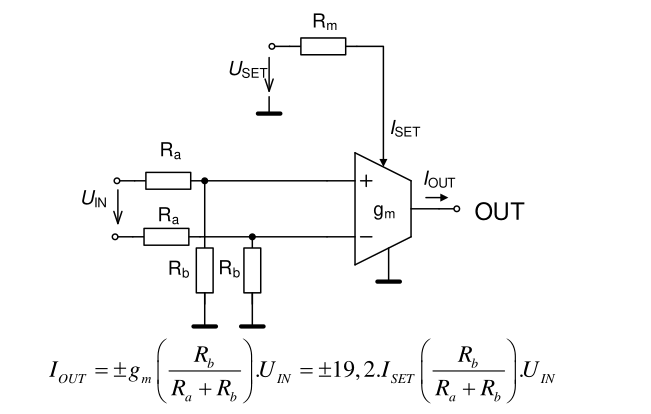
\includegraphics[width=0.5\linewidth]{Obrazky/AE2/1Otazka/zapojenieSLM13700}
\caption{Zapojenie s LM13700.}
\label{fig:zapojenieslm13700}
\end{figure}

\newpage
\chapter{Spínacie a tvarovacie obvody}
\section{Prechodové deje}
Najhoršie možné je obdĺžnikový signál / impulz - nekonečný počet harmonických zložiek $\rightarrow$ tieto signály obsahujú ostré hrany, schody a podobne $\rightarrow$ teda majú veľmi bohaté spektrum.

\textbf{Impulz:} Krátkodobá výchylka veličiny od základnej hodnoty, do ktorej sa následne vráti, jednorázová záležitosť.

\textbf{Pulz:} Opakovanie impulzov.

Pre chápanie pulzov a impulzov definujeme \textbf{typy výchyliek:} 
\begin{multicols}{2}
\begin{itemize}
	\item Jednotkový skok $\sigma$.
	\item Hodnoty:
	\begin{itemize}
		\item $\sigma = 0$ v čase $t < 0$
		\item $\sigma = 1$ v čase $t >=1$
	\end{itemize}
	\item Diracov impulz:
	\begin{itemize}
		\item Dosahuje určitej mohutnosti, je definovaný ako $\infty$ v čase $t = 0$.
		\item jedná sa o nekonečne veľký, a nekonečne úzky impulz.
		\item V praxi sa vzťahuje k jednotke.
	\end{itemize}
\end{itemize}
\end{multicols}

Reálny impulz má v prenosovej sústave exponenciálny charakter. Jednoduchá varianta je exponencionálne klesajúca tá začína jednotkovým skokom, častejšia varianta je dvojexponencionálna.

\begin{figure}[H]
\centering
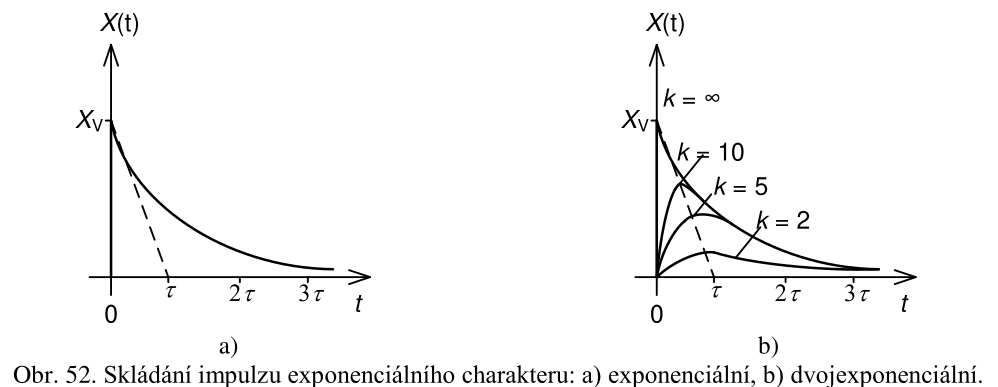
\includegraphics[width=0.6\linewidth]{Obrazky/AE2/2otazka/impulzy}
\caption{Zobrazenie impulzov.}
\label{fig:impulzy}
\end{figure}
\begin{equation}
\underset{\text{Exponenciálny impulz}}{x(t) = \sigma(t) \cdot X_V \cdot \exp\left(\frac{-t}{\tau}\right)} 
\qquad \text{a} \qquad 
\underset{\text{Dvoj-exponenciálny impulz}}{x(t) = \sigma(t) \cdot X_V \cdot \left[\exp\left(\frac{-t}{\tau}\right) - \exp\left(\frac{-k\cdot t}{\tau}\right)\right]}
\end{equation}
Kde $\tau$ predstavuje časovú konštantu - vyjadrujúcu čas potrebný pre zmenu hodnoty o \qty{63}{\%}. Či už pre pokles alebo nárast z pôvodnej hodnoty.

Prechodové deje sú popísané exponenciálnymi rovnicami. Tento popis súvisí s možnosťou transformácie správania medzi frekvenčnou a časovou oblasťou. Transformácia sa robí cez transformátorový slovník.
\begin{figure}[H]
\centering
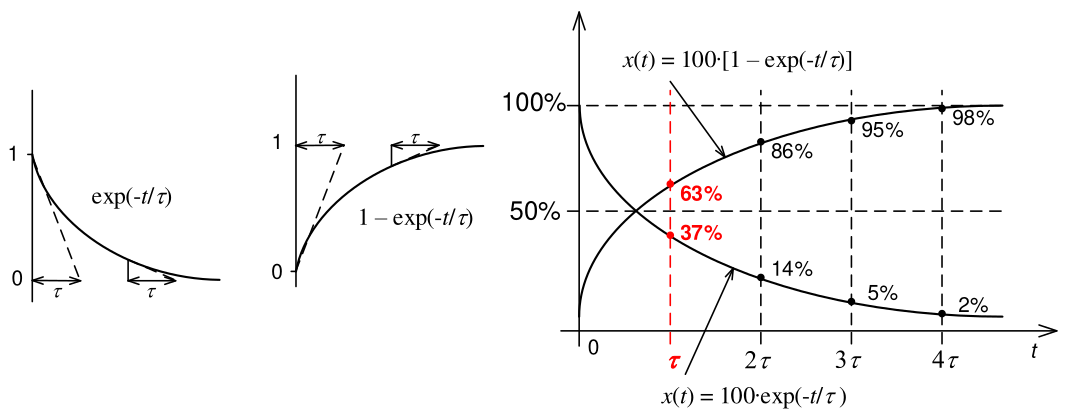
\includegraphics[width=0.7\linewidth]{Obrazky/AE2/2otazka/NormovanyPriebehExpFunkcii}
\caption{Normovaný priebeh exponenciálnych funkcií}
\label{fig:normovanypriebehexpfunkcii}
\end{figure}
Vzťah pre čas medzi dvoma úrovňami vieme definovať ako:
\begin{equation}
\Delta t = \tau \cdot \ln\left(\frac{x(\infty) - x(t_1)}{x(\infty) - x(t_2)}\right)
\end{equation}
Reálny obdĺžnikový impulz v prenosovom systéme vyzerá:
\begin{figure}[H]
\centering
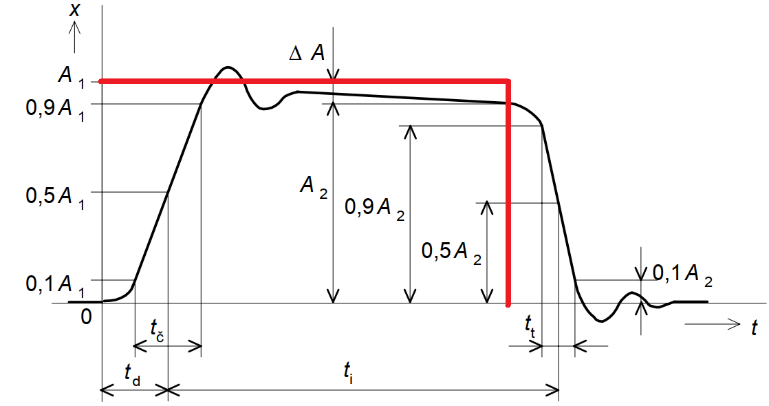
\includegraphics[width=0.7\linewidth]{Obrazky/AE2/2otazka/pravouhlyImpulz}
\caption{Porovnanie reálneho a pravoúhleho impulzu}
\label{fig:pravouhlyimpulz}
\end{figure}
Definuje sa:
\begin{itemize}
\item Doba hrany - $t_e$ resp. $t_r$ - Doba od \qty{10}{\%} po \qty{90}{\%} signálu.
\subitem \begin{equation}
	t_e = t_{0.9x} - t_{0.1x} = \tau \ln\left(\frac{x - 0,1x}{x - 0,9x}\right) = \tau \ln\left(\frac{0.1}{0.9}\right) = \tau\ln\left(9\right) \approx 2,2\tau´
\end{equation}
\item Strieda pulzu - pomer medzi aktívnou a pasívnou dobou.	
\end{itemize}
\section{Prenos lineárnou sústavou}
Lineárne články prenášajú široké spektrum frekvencií impulzov, toto spektrum je samozrejme obmedzené. Obmedzenie šírky prenášaného pásma spôsobuje lineárne skreslenie. Toto skreslenie je frekvenčne závislé, pričom nemôžu vznikať nové, pôvodne neprítomné frekvencie. V lineárnom systéme platí princíp superpozície. Signál sa oneskoruje o:
\begin{itemize}
\item Doba oneskorenia $t_d$, súvisí s lineárnym skreslením - Doba od \qty{0}{\%} po \qty{50}{\%} signálu. \textbf{Presný vzťah Platí len ak nemáme kaskádu, inak je približný.}
\subitem \begin{equation}
	t_e = t_{0.5x} - t_{0x} = \tau \ln\left(\frac{x - 0x}{x - 0,5x}\right) = \tau \ln\left(\frac{1}{0.5}\right) = \tau\ln\left(2\right) \approx 0,69\tau
	\label{eqv:38}
\end{equation}
\item Doba trvania impulzu $t_i$ - definovaná medzi \qty{50}{\%} úrovne impulzu.
\end{itemize}

Jednoduchý lineárny článok sa dá modelovať RC článkom. Definuje sa tu medzná frekvencia.
\begin{equation}
\underset{\text{Vzťah medzi dobou hrany a medznou frekvenciou.}}{t_e \approx \frac{0,35}{f_m}}
\label{eqv:teFm}
\end{equation}
Pričom doba hrany je daná vzťahom \ref{eqv:38}. Vzťah \ref{eqv:teFm} platí presne pre dolnú priepusť, približne aj pre zložitejšie obvody. Celková doba hrany bude geometrickým súčtom doby hrany článku a pôvodnej doby hrany.
\begin{equation}
t_{eo} \approx \sqrt{t_{ei}^2 + t_{e}^2} = \sqrt{t_{ei}^2 + \left(\frac{0,35}{fm}\right)^2}
\end{equation}
\subsection{Kaskáda lineárnych článkov}
Pokiaľ máme kaskádu článkov, ktoré sú od seba impedančne oddelené (Buffers), tak je to stále geometrický súčet.
\begin{figure}[H]
\centering
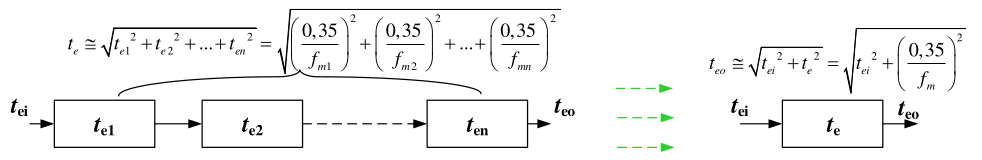
\includegraphics[width=0.9\linewidth]{Obrazky/AE2/2otazka/kaskadaClankov}
\caption{Samostatný lineárny prenosový článok a kaskáda prenosových článkov.}
\label{fig:kaskadaclankov}
\end{figure}
\begin{figure}[H]
\centering
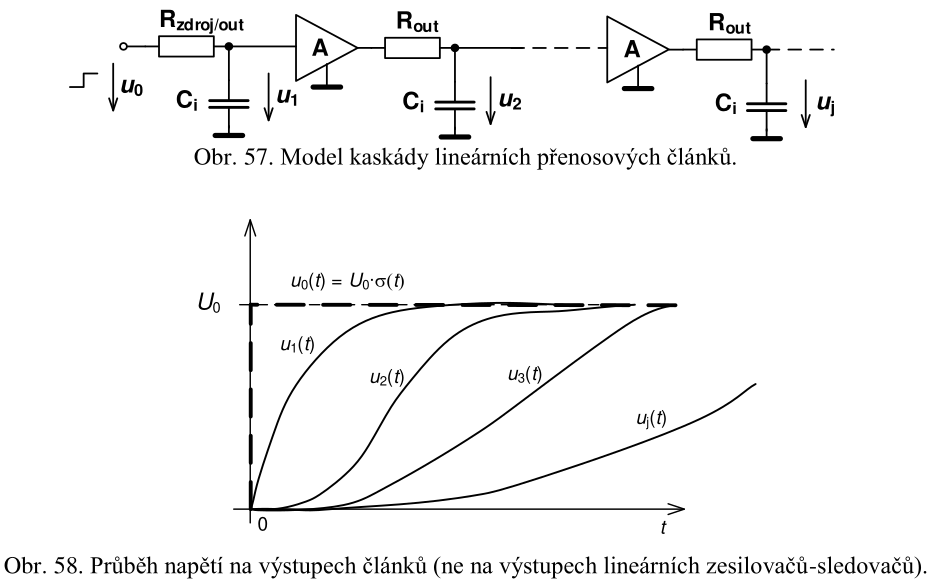
\includegraphics[width=0.7\linewidth]{Obrazky/AE2/2otazka/kaskadaClankovModel}
\caption{Model a časové priebehy článkov}
\label{fig:kaskadaclankovmodel}
\end{figure}
\textit{Poznámka: Ak jednotlivé články majú prenos iný ako 1 tak to ovplyvní aj ustálenie výstupnej úrovne kaskády.}

\section{Prenos nelineárnou sústavou}
Dochádza tu k nelineárnemu skresleniu, môžu sa objavovať nové spektrálne zložky, neplatí tu princíp superpozície. Vplývajú tu parazitné kapacity. Vlastnosti nelineárneho skreslenia:
\begin{itemize}
\item Výstupný signál obsahuje nové spektrálne zložku
\item Neplatí princíp superpozície
\item Dochádza k spojitému/nespojitému obmedzeniu signálu - prejavuje sa v nelinearite prevodnej charakteristiky
\item Dôležitý vplyv parazitných kapacít
\item Hysteréza
\end{itemize}
Vplyvom parazitných kapacít sa bude predlžovať doba hrany pôvodného signálu. Každý článok predĺži hranu. 
\underline{Maximálna dĺžka hrany je obmedzená kvôli zosilneniu!} Naopak, pokiaľ je hrana pôvodného signálu dlhá, tak po prechode kaskádou bude vplyvom zosilnenia kratkšia! Doba hrany sa po prechode niekoľkých blokov v kaskáde ustáli. $\rightarrow$ \textbf{Vlastná doba hrany}
\begin{itemize}
	\item Doba za ktorú sa ustáli doba hrany na základe relácií medzi zosilnením a zotrvačnými prvkami.
\end{itemize}

Predstava o vlastnej dobe platí len kým nedojde k rozkmitaniu zosilňovača $\rightarrow$ k tomuto dochádza pokiaľ je dĺžka pôvodnej hrany príliš veľká. Pri lineárnych prenosových článok s OZ musíme kompenzovať frekvenčnú charakteristiku zosilňovačov. Pri digitálnych sústavách stačí zaistiť dostatočne krátku hranu signálu, pri ktorých sa nemá hradlo čas rozkmitať.

\section{Integračný dvojbran - RC - dolná priepusť}
\begin{itemize}
	\item RC článok
	\item Časová konštanta: $\tau = RC$
	\item Neprenáša skokové zmeny
	\item Pri vstupnom harmonickom signále $\rightarrow$ signál fázovo posunutý o \qty{-90}{\degree} (Ak sedí frekvencia pre -3dB)
	\item Pri vstupnom obdĺžniku s kratšou periódou ako $\tau$ $\rightarrow$ výstup je trojuholník
	\item Potrebné uvažovať pripojené zariadenia - ak má zdroj signálu výstupný odpor, či záťaž článku kapacitný charakter $\rightarrow$ ovplyvňuje to $\tau$!
	\item Pokiaľ je článok zaťažený porovnateľným odporom $\rightarrow$ vytvorí sa paralelná kombinácia odporov $\rightarrow$ ovplyvní to výslednú úroveň napätia (Odporový delič) $\rightarrow$ a aj $\tau$!
\end{itemize}
\begin{figure}[H]
	\centering
	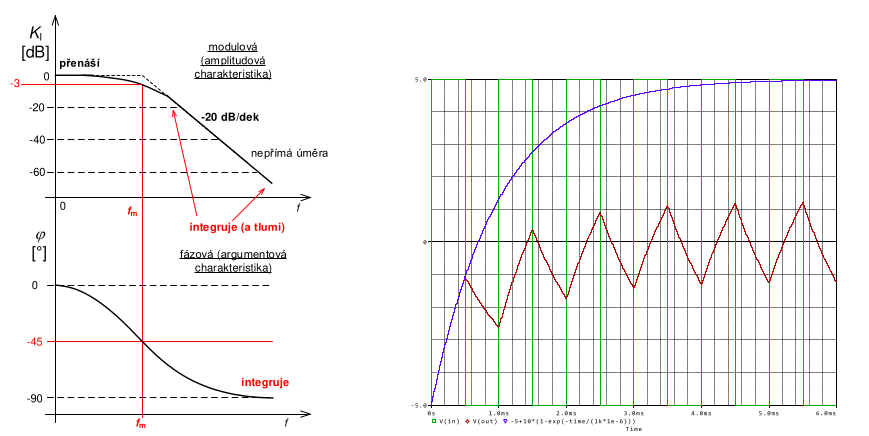
\includegraphics[width=0.7\linewidth]{Obrazky/AE2/2otazka/integracnyClanok}
	\caption{Príklad integračného procesu pre periódu vstupného signálu nižšiu ako $\tau$.}
	\label{fig:integracnyclanok}
\end{figure}
Integračný článok sa vyskytuje bežne ako forma parazity. Vytvorí sa jednoducho z výstupného odporu zdrojov a vstupných kapacít pripojených zariadení. Vytvára sa teda lineárne skreslenie signálu.

\textit{Poznámka: V prípade, že vstupný signál je hlboko v útlme \qty{-20}{dB/dec}, dochádza k stratovej integrácií $\rightarrow$ ak chceme bezstratový integrátor, musíme doplniť obvod aktívnym prvkom}
\begin{figure}[H]
	\centering
	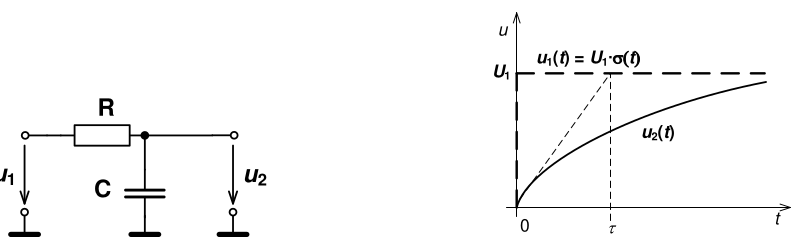
\includegraphics[width=0.7\linewidth]{Obrazky/AE2/2otazka/integracnyClanokzapojenie}
	\caption{Zapojenie integračného článku}
	\label{fig:integracnyclanokzapojenie}
\end{figure}

\section{Derivačný dvojbran - CR - horná priepusť}
\begin{itemize}
	\item CR článok
	\item Neprenáša jednosmernú zložku
	\item Časová konštanta: $\tau = CR$
	\item Pre nízke lineárne skreslenie musí byť $\tau >>$ ako šírka impulzu, čím väčší je tento rozdiel, tým kvalitnejšia derivácia.
	\item Pri vstupnom harmonickom signále $\rightarrow$ signál fázovo posunutý o \qty{90}{\degree} (Ak sedí frekvencia pre -3dB)
	\item Pri vstupnom obdĺžniku $\rightarrow$ výstup je 0 (DC zložku ee)
	\item Pri vstupnom trojuholníku $\rightarrow$ výstup je obdĺžnik
	\item \underline{Pokiaľ je zaťažený zotrvačnou záťažou, dochádza k zmene rádu článku!} (Kapacitná záťaž $\rightarrow$ Wienov článok $\rightarrow$ 2. rád)
\item Pokiaľ je pripojený na zdroj s nenulovým výstupným odporom a je k nemu pripojená rezistívna záťaž, jeho výstupné napätie je dané vytvoreným odporovým deličom.
\item Vyskutuje sa v podobe parazít medzi cestami DPS, rovnako sa s ním stretávame ako s oddeľovačom jednosmernej zložky.
\item Časová konštanta $\tau$, ovplyvňuje prenos rušivého signálu $\rightarrow$ nižžsie $\tau$, nižšie rušenie.
\end{itemize}
\textit{Poznámka: Pokiaľ sa pohybujeme v útlme, jedná sa o stratový derivačný článok}
\begin{figure}[H]
	\centering
	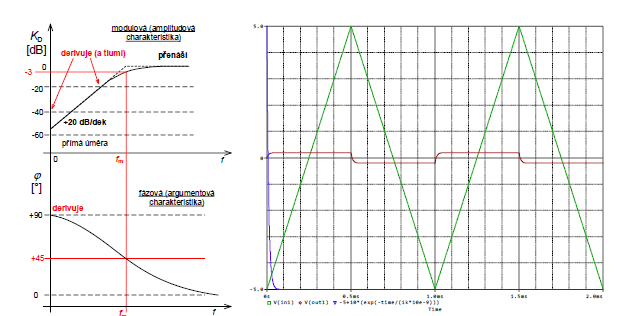
\includegraphics[width=0.7\linewidth]{Obrazky/AE2/2otazka/derivacnyClanok}
	\caption{Príklad derivačného procesu stratového derivátora}
	\label{fig:derivacnyclanok}
\end{figure}
\begin{figure}[H]
	\centering
	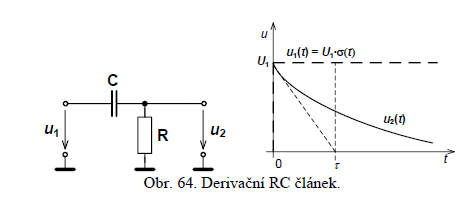
\includegraphics[width=0.7\linewidth]{Obrazky/AE2/2otazka/derivacnyClanokzapojenie}
	\caption{Zapojenie derivačného článku}
	\label{fig:derivacnyclanokzapojenie}
\end{figure}
\section{Frekvenčne závislý delič napätia}
Bavíme sa o pasívnych osciloskopických sondách.

Ideálny delič nie je frekvenčne závislý, len zníži úroveň napätia $\rightarrow$ teda nemení tvar pôvodného signálu. V realite sa však prejavuje kapacita záťaže, vznikajúca parazitnou kapacitou spojov, či vstupnou kapacitou naväzujúceho obvodu $\rightarrow$ vzniká integračný článok $\rightarrow$ delič tlmí VF zložky signálu.

Pokiaľ nechceme dopustiť toto tlmenie, musí sa delič kompenzovať. Kompenzácia sa robí paralelným kondenzátorom. Napriek tomu, to nie je obvod druhého rádu, nakoľko z pohľadu zdroja sú paralelne. Pre správne kompenzovaný delič platí, že prenos ustálenej zložky a zmeny je rovnaký \(d_R = d_C\): 
\begin{equation}
	\tau_1 = \tau_2 \implies R_1 C_1 = R_2 C_2
\end{equation}
\begin{figure}[H]
\centering
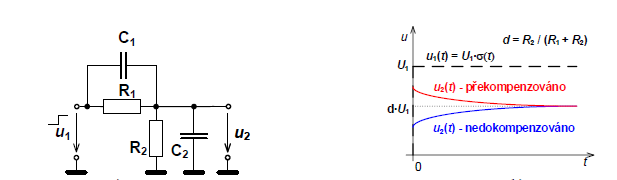
\includegraphics[width=0.7\linewidth]{Obrazky/AE2/2otazka/frekZavisDelic}
\caption{Kompenzácia deliča}
\label{fig:frekzavisdelic}
\end{figure}
V ideálnom svete, by vstupný impulz znamenal teoreticky nekonečný prúd (kondenzátory by sa museli nabiť okamžite). To však nie je možné, je to limitované výstupným odporom zdroja signálu. Vtedy sa už jedná o obvod 2. rádu.
\begin{figure}[H]
	\centering
	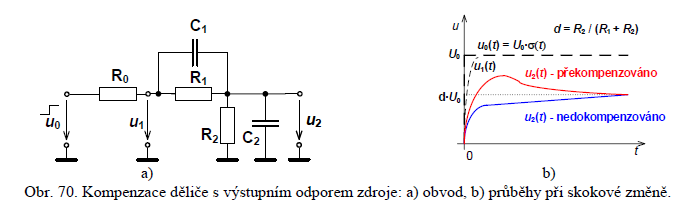
\includegraphics[width=0.7\linewidth]{Obrazky/AE2/2otazka/frekZavisDelicVystupnyOdpor}
	\caption{Kompenzácia deliča s výstupným odporom zdroja signálu}
	\label{fig:frekzavisdelicvystupnyodpor}
\end{figure}
\section{Diódové funkčne meniče}
Jedná sa o nelineárne obvody určené na tvarovanie či orezávanie signálu v časovej oblasti. Využíva sa vedenie prúdu diódou len jedným smerom. 
\subsection{Diódový obmedzovač}
\begin{itemize}
	\item Delič napätia s nelineárnym prvkom
	\item Minimálna hodnota napätia je daná PN prechodom diódy $\rightarrow$ cca \qty{0.6}{\V} čo môže byť problém
	\item V prípade, že chceme obmedziť vyššie napätie ako je \qty{0.6}{\V} môžeme to urobiť pridaním zdroja napätia sériovo s diódou $\rightarrow$ efektívne sa posunie hranica orezávania o hodnotu priloženého napätia.
	\subitem Zdroj napätia vieme riešiť napríklad buffrom, ktorý má \emph{umelú zem}
\end{itemize}
\begin{figure}[H]
	\centering
	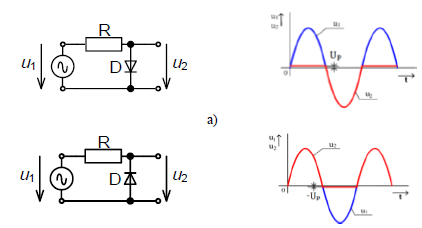
\includegraphics[width=0.7\linewidth]{Obrazky/AE2/2otazka/diodovyObmedzovac}
	\caption{Príklad diódového obmedzovača}
	\label{fig:diodovyobmedzovac}
\end{figure}
\begin{figure}[H]
	\centering
	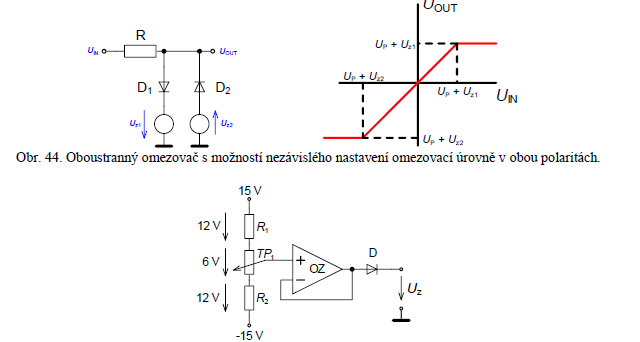
\includegraphics[width=0.7\linewidth]{Obrazky/AE2/2otazka/diodovyObmedzovacObojsmerny}
	\caption{Obojsmerný diódový obmedzovač}
	\label{fig:diodovyobmedzovacobojsmerny}
\end{figure}
\subsection{Diódový vykrajovač}
\begin{itemize}
	\item Úlohou je vykrojiť len časť priebehu.
	\item Nesleduje sa napätie ale sleduje sa prúd pretekajúci diódou.
	\item Znovu je možné stanoviť hodnoty vykrajovania pre obe polarity vstupného napätia.
	\item Strmosť výstupnej charakteristiky je daná odporom $R_5$
	\item Z princípu je výstupný signál invertovaný
\end{itemize}
\begin{figure}[H]
	\centering
	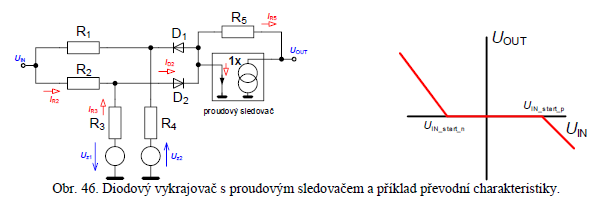
\includegraphics[width=0.7\linewidth]{Obrazky/AE2/2otazka/diodovyVykrajovac}
	\caption{Ukážka diódového vykrajovača}
	\label{fig:diodovyvykrajovac}
\end{figure}
\subsection{Diódový tvarovač}
\begin{itemize}
	\item Jedná sa o funkčný meniť.
	\item Používa sa pre aproximáciu harmonického signálu $\rightarrow$ metódou lomených priamok.
	\item Spracováva pílový vstupný signál, pričom frekvencia je obmedzená len parazitnými kapacitami obvodu.
	\item Nesmie sa meniť vstupná amplitúda signálu.
	\item Môže byť nepraktické pre malé signály.
	\item Polperiódu signálu je nutné rozdeliť na nepárny počet úsekov $\rightarrow$ inak by vznikla v maxime ostrá špička $\rightarrow$ počet úsekov je rovný počtu segmentov diódového tvarovača.
	\item Jedná sa znovu o odporový delič, pričom jeho odpory sa menia podľa otvárania diód $\rightarrow$ mení sa strmosť výstupu.
	\item Vzdialenosti medzi úsekmi sa dajú aproximovať rôzne, napríklad ekvidistantnou vzdialenosťou medzi hranicami.
\end{itemize}
\begin{figure}[H]
	\centering
	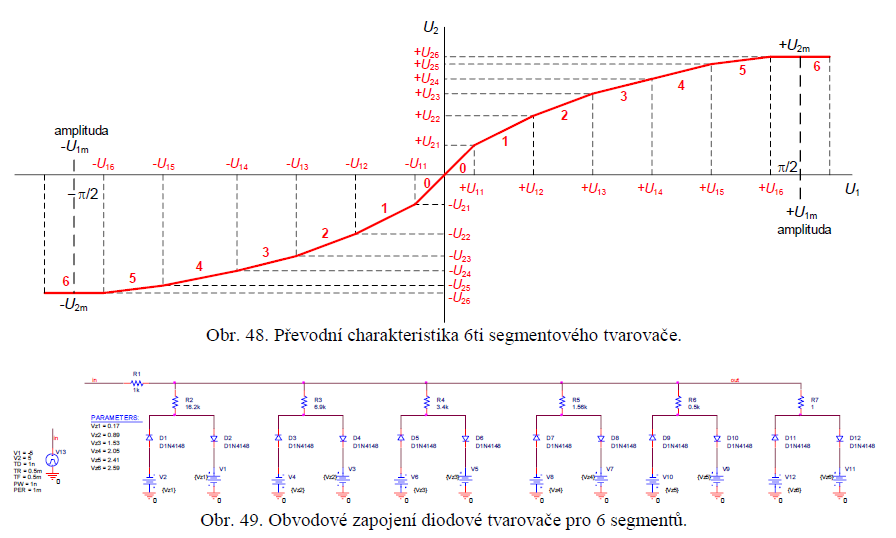
\includegraphics[width=0.9\linewidth]{Obrazky/AE2/2otazka/diodovyTvarovac}
	\caption{Ukážka prevodnej charakteristiky a zapojenia šesť segmentového diódového tvarovača.}
	\label{fig:diodovytvarovac}
\end{figure}
\section{Bipolárny tranzistorový spínač}
\begin{itemize}
	\item Návrh podstatne zložitejší ako pri Unipolárnych spínačoch
	\item Pri návrhu sa nedajú aplikovať malosignálové úvahy
	\item Na návrh jedného stupňa stačí v podstate len bázový odpor, ktorý nastaví potrebný prúd do báze, pre dosiahnutie požadovaného prúdového zosilnenia
	\item Viacstupňový návrh je v podstate dynamické spínanie odporových deličov, kedy jeden stupeň spína odporový delič na svojom výstupe a tým nastavuje pracovné podmienky pre spustenie ďalšieho stupňa.
	\item Celý návrh je v podstate len odhad, nakoľko sa robí podstatne zjednodušený.
	\item Pri návrhu sa nedá uvažovať konštantný parameter $\beta$ $\rightarrow$ teda prúdový zosilovací činiteľ, nakoľko je závislý od kolektorového prúdu a teploty tranzistora.
	\subitem Navyše majú výkonové spínacie prvky podstatne nižšie hodnoty tohto činiteľa.
	\item Stručný postup návrhu:
	\begin{enumerate}
		\item Začína sa od konca $\rightarrow$ od záťaže, kedy na základe potrebného spínaného prúdu zistíme potrebný bázový prúd
		\item Pokračuje sa výpočtom deliča na vstupe posledného stupňa.
		\item Výpočet deliča závisí na prúde kolektorom predchádzajúceho stupňa
		\subitem a takto sa to točí xD :kappa: :vutEz:
	\end{enumerate}
	\item V procese návrhu je nutné využívať antisaturačné diódy, zapojené medzi bázu a kolektor.
	\subitem Ich úlohou je zaistiť aby nekleslo kolektorové napätie pod bázové napätie $\rightarrow$ dochádza k hlbokej saturácií.
	\subitem Dióda urýchľuje dobu spínania, no zvyšuje parazitnú kapacitu medzi C-B.
	\subitem Používajú sa Schottkyho diódy.
	\item Tento návrh má aj iné problémy:
	\subitem Saturačný úbytok napätia $\rightarrow$ pri veľkých prúdoch sa to bude hriať jak prasa na ražni
	\subitem Prúd do báze môže neprimerane zaťažovať riadiaci obvod
\end{itemize}
\begin{figure}[H]
	\begin{subfigure}[b]{0.48\textwidth}
		\centering
		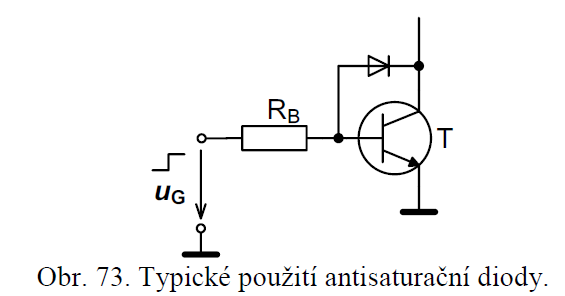
\includegraphics[width=0.7\linewidth]{Obrazky/AE2/2otazka/anitsaturacnaDioda}
		\caption{Príklad zapojenia antisaturačnej diódy}
		\label{fig:anitsaturacnadioda}
	\end{subfigure}
	\begin{subfigure}[b]{0.48\textwidth}
		\centering
		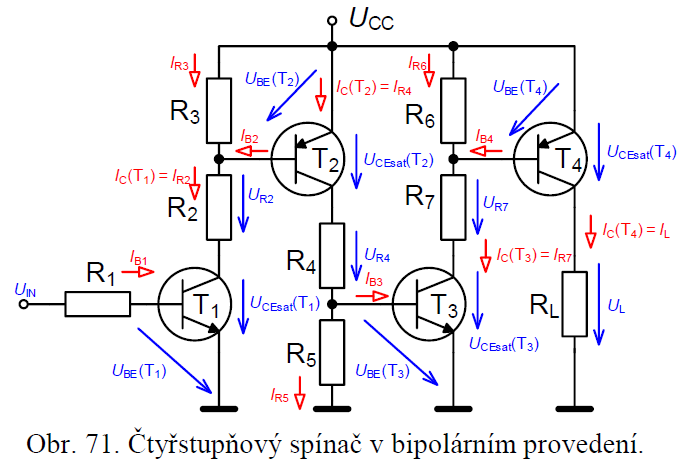
\includegraphics[width=0.7\linewidth]{Obrazky/AE2/2otazka/stvorstupnovySpicna}
		\caption{Príklad zapojenia štvorstupňového bipolárneho spínača}
		\label{fig:stvorstupnovyspicna}
	\end{subfigure}
\end{figure}
\section{Unipolárny tranzistorový spínač}
\begin{itemize}
	\item Jednoduché na návrh.
	\item Netrpí neduhmi bipolárnej štruktúry - menšie straty vďaka nízkemu odporu kanálu.
	\item Na druhú stranu majú výkonové unipolárne prvky majú vysokú kapacitu medzi G-S.
	\item Vysoká kapacita G-S znamená, že v okamihu vypnutia sú potrebné vysoké prúdy pre vybitie tejto kapacity
	\item Častokrát sa používajú takzvané Drivers
	\begin{itemize}
		\item Úloha Driver-u je jasná $\rightarrow$ urýchliť spínanie a odpínanie MOS.
	\end{itemize}
	\item V podstate je všetko EZ a pohodka
\end{itemize}
\begin{figure}[H]
	\centering
	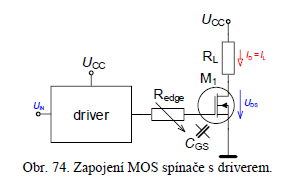
\includegraphics[width=0.5\linewidth]{Obrazky/AE2/2otazka/mosfetSpinac}
	\caption{Príklad zapojenia MOSFET spínača.}
	\label{fig:mosfetspinac}
\end{figure}
\section{Zdroje zákmitov}
\begin{itemize}
	\item Rýchle spínanie vyvoláva rezonančné zákmity $\rightarrow$ spôsobené parazitnou indukčnosťou a kapacitou v obvode $\rightarrow$ od stoviek kHz
	\item Pri veľkých záťažiach je to len viac problematické, je problém prekonať \qty{1}{\MHz}
	\item Rezonančná frekvencia zákmitov je daná Tompsonovým vzťahom \(f_{rez} = \frac{1}{2\pi \sqrt{L_p C_p}}\)
	\item Proti zákmitom sa dá bojovať s využitím \emph{Snubberu}, čo je paralelný RC obvod, pripojený k spínaciemu prvku
	\subitem Jeho princíp využíva vzájomné predávanie energie medzi cievkou a kondenzátorom
\end{itemize}
\begin{figure}[H]
	\centering
	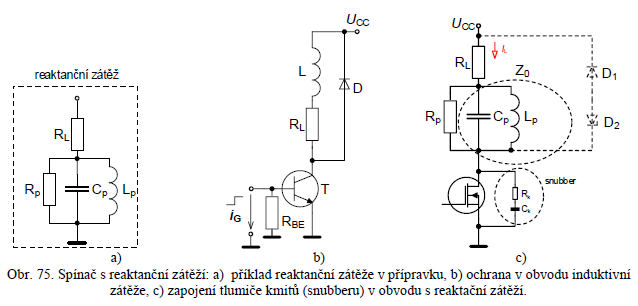
\includegraphics[width=0.7\linewidth]{Obrazky/AE2/2otazka/zdrojeZakmitov}
	\caption{Reaktančná záťaž a obrany voči zákmitom}
	\label{fig:zdrojezakmitov}
\end{figure}
Princíp návrhu \emph{snubberu}: (Písalo to AI)
\begin{itemize}
	\item \textbf{Hodnota rezistora $R_k$:} Musí sa pohybovať okolo charakteristickej impedancie obvodu, teda $R_k \le Z_0 = \sqrt{L_p/C_p}$, prípadne podľa zjednodušeného odhadu $R_k \le U_{CC}/I_L$.
	\item \textbf{Dimenzovanie rezistora $R_k$:} Musí byť schopný odolať špičkovému napätiu zodpovedajúcemu $U_{CC}$ v rozopnutom stave (OFF) a špičkovému prúdu zodpovedajúcemu prevádzkovému prúdu v zopnutom stave (ON).
	\item \textbf{Minimálna kapacita $C_k$:} Energia uložená v kondenzátore musí byť väčšia ako energia indukčnosti obvodu, z čoho vyplýva podmienka $C_{kmin} > L_p \cdot I_L^2 / U_{CC}^2$.
	\item \textbf{Časová konštanta obvodu:} Časová konštanta snubbra musí byť menšia ako desatina doby aktívneho stavu spínača, teda $R_k \cdot C_{kmax} < t_{on}/10$.
	\item \textbf{Celkový rozsah kapacity $C_k$:} Kapacita kondenzátora musí spĺňať výsledné operatívne rozmedzie: $\frac{L_p \cdot I_L^2}{U_{CC}^2} < C_k < \frac{t_{on}}{10}$.
	\item \textbf{Ochrana pri spínaní induktívnej záťaže:} Je nutné paralelne k záťaži pripojiť výkonovú diódu (prípadne v kombinácii so Zenerovou diódou), ktorá zamedzí prekmitom napätia nad úroveň $U_{CC}$ a ochráni spínač pred prekročením maximálnej straty.
	\item \textbf{Dimenzovanie ochranných diód:} Špičky prúdu tečúceho ochrannými diódami nesmú prekročiť ich maximálny povolený stratový príkon, inak je potrebné použiť zrážací odpor alebo zvoliť robustnejší typ diód.
\end{itemize}
\section{Výkonové straty pri spínaní}
\begin{itemize}
	\item  Straty na bipolárnej štruktúre:
	\begin{itemize}
		\item rozdeľujú sa na vstupné a výstupné
		\item vstupné
		\begin{itemize}
			\item Bázové straty - väčšinou zanedbateľné, kým bázou netečú veľké prúdy
		\end{itemize}
		\item výstupné
		\begin{itemize}
			\item statické (pri stabilnom stave zopnutého tranzistora)
			\subitem Jedná sa o súčin saturačného napätia tranzistora a prúdu kolektorom.
			\item dynamické (pri pravidelnom spínaní)
			\subitem napätia a prúdy v okamihu zopnutia či rozopnutia narastajú / klesajú exponencionálne
		\end{itemize}
	\end{itemize}
	\item  Straty na unipolárnej štruktúre:
	\begin{itemize}
		\item Vďaka malému odporu kanálu sú straty mizivé (pri nízkych prúdoch)
		\item Statické straty sa riadia podobne ako pri BJT
		\item Dynamické straty sú tiež podobné
	\end{itemize}
\end{itemize}
\section{Klopné obvody}
Rozlišujú dva typy stavov $\rightarrow$ stabilný a nestabilný stav. Prechod medzi stabilnými stavmi sa nazýva nestabilný stav. Základom klopných obvodov sú zosilňovače s kladnou spätnou väzbou. To sa dá realizovať tranzistorovými stupňami, minimálne dva. Podľa charakteru stabilných stavov rozlišujeme:
\begin{itemize}
	\item Bistabilný KO - oba stavy sú trvalo stabilné.
	\item Monostabilný KO - jeden stav je trvalo a druhý je dočasne stabilný.
	\item Astabilný KO - oba stavy sú dočasne stabilné, obvod nimi prechádza dookola.
	\item Dá sa realizovať z tranzistorov, z NOR hradiel, rovnako aj RS-KO obvod (pri vylúčení možnosti aktivácie R a S vstupov naraz)
\end{itemize}

\subsection{Bistabilný klopný obvod}
\begin{itemize}
	\item Pozostáva z dvoch tranzistorových stupňov s DC väzbou.
	\item Na zmenu stavu je potrebný vonkajší vstup.
	\item Tvoria základ pre registry, čítače a podobne.
\end{itemize}
\begin{figure}[H]
	\centering
	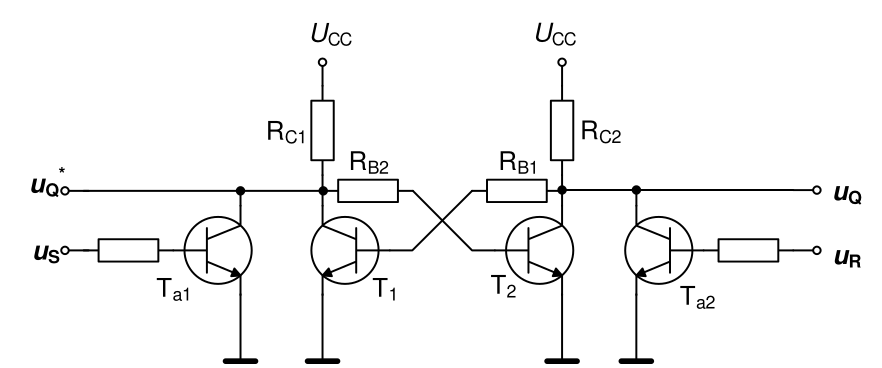
\includegraphics[width=0.7\linewidth]{Obrazky/AE2/2otazka/bkotrans}
	\caption{Bistabilný klopný obvod z tranzistorov}
	\label{fig:bkotrans}
\end{figure}
\begin{figure}[H]
	\centering
	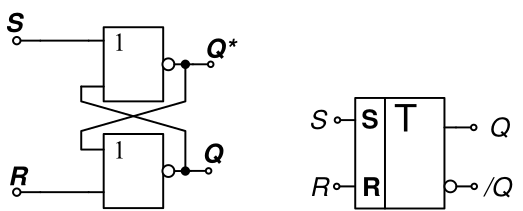
\includegraphics[width=0.45\linewidth]{Obrazky/AE2/2otazka/bkoLogi}
	\caption{Realizácia Bistrabilného klopného obvodu z NOR hradiel a RS-KO}
	\label{fig:bkologi}
\end{figure}
\subsection{Monostabilný klopný obvod}
\begin{itemize}
	\item Zapojenie vychádza zo zapojenia BKO, jedna spätná väzba je viazaná kondenzátorom.
	\item Po privedení napájacieho napätia je T2 otvorené T1 uzavreté. Kondenzátor C je nabitý na $U{CC}-U_{BE_{satT2}}$
	\item Spúšťací impulz skratne kolektor T1, spustí sa prebíjanie kondenzátora, T2 ostane uzavretý do doby kým sa napätie na C nevráti na pôvodnú úroveň.
	\item Časová konštanta $\tau = R_{B2} C$
	\item Doba zotavenia $t_i = \ln(2)\tau$
	\item Klasické MKO reaguje na spúšťací impulz len pokiaľ je v stabilnom stave.
	\item Existujú aj znovu spustiteľné MKO, ktoré zakaždým resetujú dobu zotavenia.
	\item Je možná realizácia aj s 555 časovačom.
\end{itemize}
\begin{figure}[H]
	\centering
	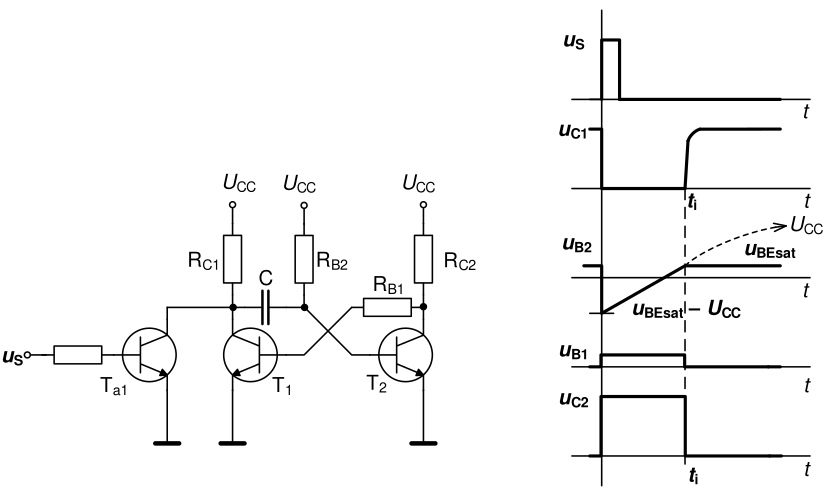
\includegraphics[width=0.55\linewidth]{Obrazky/AE2/2otazka/mkoTrans}
	\caption{Zapojenie MKO spolu s časovými pribehmi.}
	\label{fig:mkotrans}
\end{figure}
\begin{figure}[H]
	\centering
	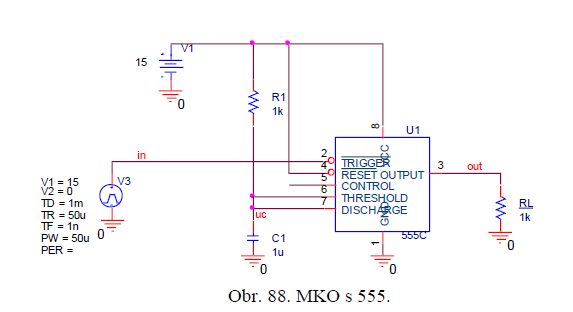
\includegraphics[width=0.7\linewidth]{Obrazky/AE2/2otazka/mko555}
	\caption{Realizácia MKO s časovačom 555, $t_i = \tau \ln(3)$}
	\label{fig:mko555}
\end{figure}
\subsection{Astabilný klopný obvod} 
\begin{itemize}
	\item Vychádzajú z MKO, kedy sú obe spätné väzby nahradené kondenzátorovou väzbou.
	\item Neustále sa preklápajú, nemajú spúšťací impulz, potrebujú len napájanie.
	\item Používajú sa na ľahké generovanie pravouhlých impulzov.
	\item V RF technike sa z nich po filtrácií dá generovať aj harmonický signál.
	\item Možná realizácia aj s časovačom 555.
	\item Nastavenie periódy je možné: 
	\item \[T = t_1 + t_2 = (R_{B1} C_1 + R_{B2} C_2) \ln(2) = \frac{1}{f_0}\]
\end{itemize}
\begin{figure}[H]
	\centering
	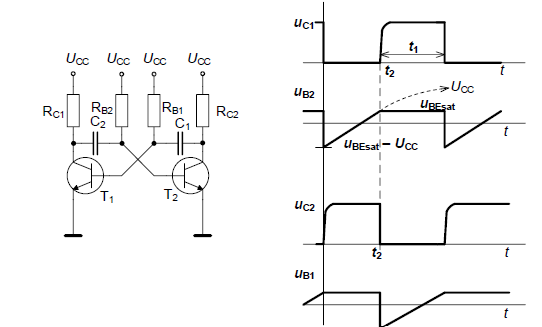
\includegraphics[width=0.55\linewidth]{Obrazky/AE2/2otazka/akoTrans}
	\caption{Zapojenie AKO spolu s časovými priebehmi.}
	\label{fig:akotrans}
\end{figure}
\begin{figure}[H]
	\centering
	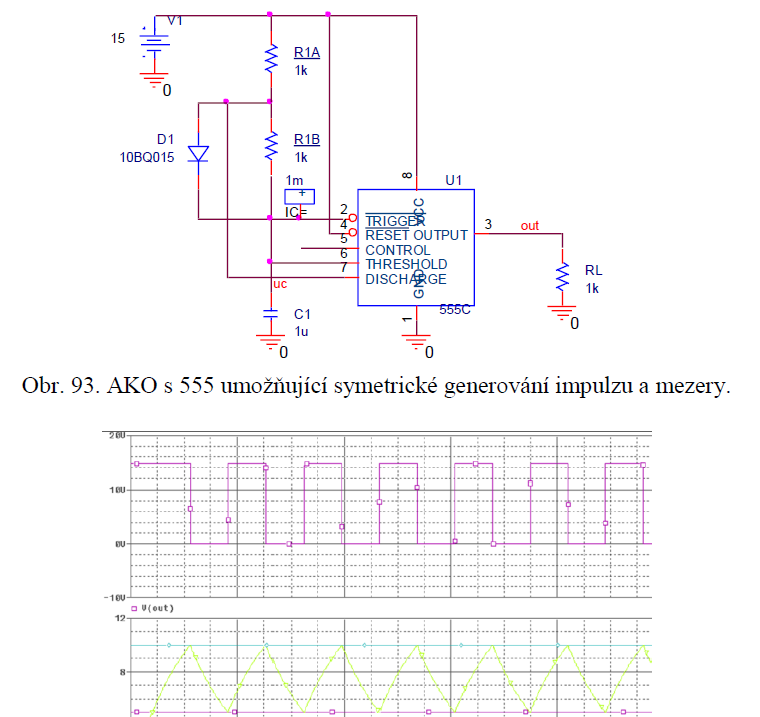
\includegraphics[width=0.7\linewidth]{Obrazky/AE2/2otazka/ako555}
	\caption{AKO s časovačom 555}
	\label{fig:ako555}
\end{figure}
\subsection{Klopné obvody s logických prvkov - hradiel}
Klopný obvod je možné realizovať s RS blokom, rovnako aj s radou TTL hradiel.
\section{Komparátory}
\subsection{Tranzistor ako invertujúci komparátor}
\begin{itemize}
	\item Najjednoduchší komparátor.
	\item Z povahy je invertujúceho charakteru.
	\item Rozhodovacia úroveň napätia je daná bázovým napätím tranzistora $\rightarrow$ \qty{0.7}{\V}.
	\item Užíva sa ochranná dióda, pre ochranu voči zápornému napätiu.
	\item Nehrozí rozkmitanie, vhodný pre veľké vstupné signály.
	\item Pokiaľ vstupné napätie prechádza oblasťou rozhodovacej úrovne pomaly $\rightarrow$ dochádza k spojitej zmene výstupného napätia.
\end{itemize}
\begin{figure}[H]
	\centering
	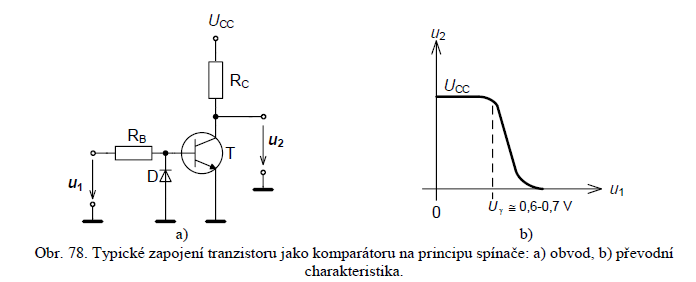
\includegraphics[width=0.55\linewidth]{Obrazky/AE2/2otazka/tranzistorInvertKomp}
	\caption{Invertujúci tranzistorový komparátor.}
	\label{fig:tranzistorinvertkomp}
\end{figure}
\subsection{Tranzistor ako neinvertujúci komparátor}
\begin{itemize}
	\item Vychádza z invertujúceho zapojenia $\rightarrow$ prosté zapojenie jednotlivých stupňov do kaskády.
	\item Dvojité zapojenie invertujúcich stupňov odstráni inverziu.
	\item Dosahuje sa vyššej úrovne zosilnenia výstupu.
	\item Nebezpečenstvo rozkmitania.
	\subitem Rozkmitanie sa dá potlačiť kladnou spätnou väzbou.
	\item KZV nám vytvorí v obvode hysterézu.
	\item S hysterézou sú zmeny napätia skokové.
	\item Nepoužívajú sa často $\rightarrow$ nemožnosť nastavenia rozhodovacej úrovne $\rightarrow$ nahradené Schmittovým komparátorom.
	\item Teplotne závislé.
\end{itemize}
\begin{figure}[H]
	\centering
	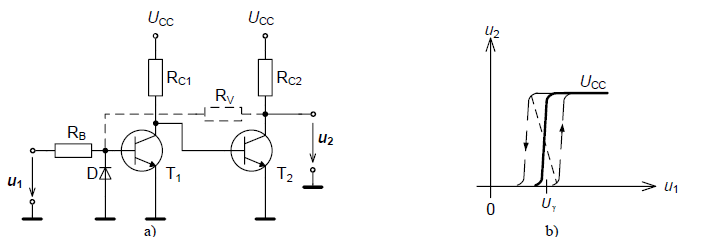
\includegraphics[width=0.55\linewidth]{Obrazky/AE2/2otazka/neinvertujuciKomparatorTrans}
	\caption{Zapojenie neinvertujúceho tranzistorového komparátora.}
	\label{fig:neinvertujucikomparatortrans}
\end{figure}
\subsection{Komparátor s diferenčným vstupom}
\begin{itemize}
	\item Zníženie teplotnej závislosti.
	\item V základnej podobe nevie robiť menej ako \qty{0.5}{\V}. Ak chceme nižšiu hodnotu potrebujeme symetrické napájanie.
	\item Nazýva sa komparačný zosilňovač.
\end{itemize}
\begin{figure}[H]
	\centering
	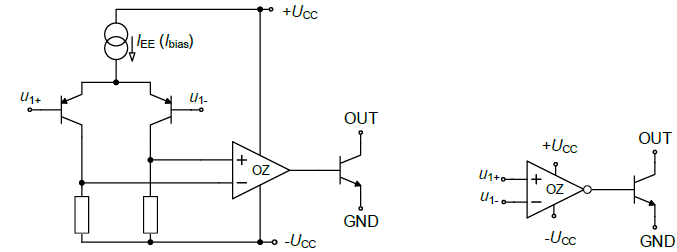
\includegraphics[width=0.55\linewidth]{Obrazky/AE2/2otazka/diferencnyKomparator}
	\caption{Typický komparátor s diferenciálnym vstupom}
	\label{fig:diferencnykomparator}
\end{figure}
\subsection{Zapojenie komparátora s komparačným zosilňovačom}
\begin{itemize}
	\item K zmene výstupu dochádza pri rovnosti vstupného napätia.
	\item Komparačné úrovne sú dané hodnotami rezistorov.
	\item Rozhodovacia úroveň je závislá na veľkosti záťaže $\rightarrow$ toto môže byť problém.
	\item Bežne sa realizujú s výstupom typu \emph{otvorený kolektor $\rightarrow$ open drain}.
	\item Má invertujúci charakter $\rightarrow$ dá sa vytvoriť aj neinvertujúci, ak sa vytvorí delič na neinvertujúcom vstupe a zavedie spätná väzba podobne ako pri dvojstupňovom tranzistorovom komparátore.
\end{itemize}
\begin{figure}[H]
	\centering
	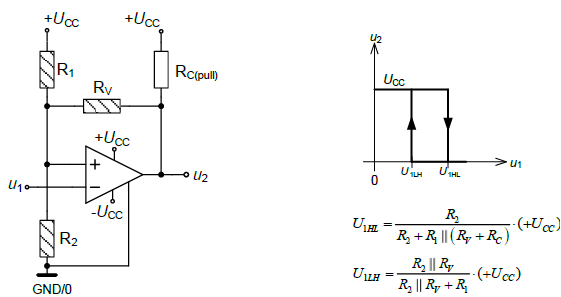
\includegraphics[width=0.55\linewidth]{Obrazky/AE2/2otazka/komparator}
	\caption{Zapojenie komparačného zosilňovača.}
	\label{fig:komparator}
\end{figure}
\section{Zapojenie OZ ako komparátora}
\begin{itemize}
	\item Klasické OZ nie sú určené na prácu v saturačnom režime.
	\item Pri návrate z nasýtenia do lineárnej oblasti sa prajavuje saturačné oneskorenie výstupu.
	\item OZ sa nehodia používať tam kde je potrebná rýchla odozva.
	\item Výhoda tohto je aj dvojčinné zapojenie výstupu, spínač na zápornú aj kladnú svorku.
	\item Výstupné napätie v saturácií sa lýši od napájacieho napätia $\rightarrow$ lepšie použiť Rail-To-Rail.
	\item Nepresnosť výstupného napätia je ovplyvnená teplotou.
\end{itemize}
\begin{figure}[H]
	\centering
	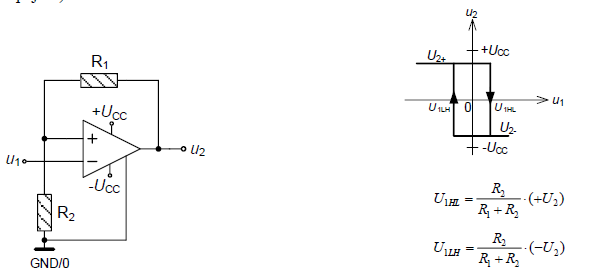
\includegraphics[width=0.7\linewidth]{Obrazky/AE2/2otazka/komparatorOZ}
	\caption{Zapojenie klasického OZ ako komparátora.}
	\label{fig:komparatoroz}
\end{figure}
\subsection{Okienkový komparátor}
\begin{itemize}
	\item Dvojica komparátorov s jednou rozhodovacou úrovňou, výstup viazaný logickým blokom.
	\item Sú potrebné dve referenčné napätia.
	\item Neivertujúce zapojenie.
	\item Rozhodovacie úrovne dané referenčným napätím, nie záťažou.
	\item Presný komparátor s hysterézou.
	\item Pri modifikácií s RS-KO je možné dosiahnuť hysterézu.
	\item Časovač 555 JE okienkový komparátor.
\end{itemize}
\begin{figure}[H]
	\centering
	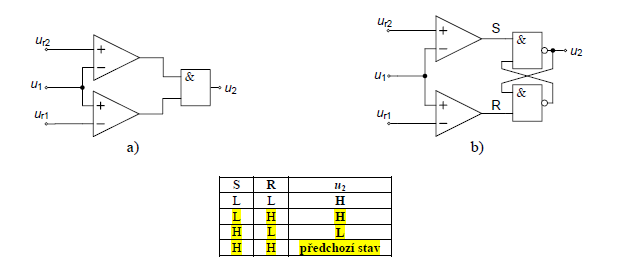
\includegraphics[width=0.7\linewidth]{Obrazky/AE2/2otazka/okienkovyKomparatro}
	\caption{Okienkový komparátor a jeho modifikácia s RS-KO}
	\label{fig:okienkovykomparatro}
\end{figure}
\begin{figure}[H]
	\centering
	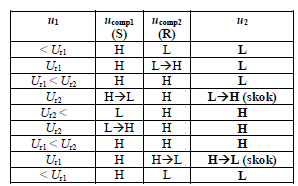
\includegraphics[width=0.7\linewidth]{Obrazky/AE2/2otazka/RSKOkomparatorStavy}
	\caption{Tabuľka stavov komparátora s RS-KO}
	\label{fig:rskokomparatorstavy}
\end{figure}
\section{Generátory priebehov}
\subsection{Relaxačný generátor $\rightarrow$ multivibrátor}
\begin{itemize}
	\item Základný blok je integračný RC článok a OZ.
	\item Komparátor musí byť invertujúcej povahy.
	\item Dosiahnutie komparačnej úrovne na vstupe vyvolá zmenu výstupu, teda ak sa kondík nabíjal, tak sa začne vybíjať.
	\item Komparačná úroveň je nastavená referenčným napätím na deliči pripojenom na neinvertujúci vstup.
	\item Po štarte obvodu je čas preklopenia výstupu $t_1$ iný ako čas po ustálení obvodu.
	\item Celá perióda opakovania je vyjadrená:
	\begin{equation}
		T = \frac{1}{f_0} = 2 R C \ln\left(\frac{R_a + 2 R_b}{R_a}\right)
	\end{equation}
	\item Vyžaduje sa symetrické napájanie $\rightarrow$ dve porovnávacie úrovne $\rightarrow$ $U_{Ref2} = -U_{Ref1}$
	\item Vyhovuje použiť Rail-To-Rail operák.
	\item Možnosť zmeny striedy výstupného signálu je ak $R_b$ neuzemníme ale posadíme ho na DC zdroj.
\end{itemize}

\begin{figure}[H]
	\begin{subfigure}[b]{0.48\textwidth}
		\centering
		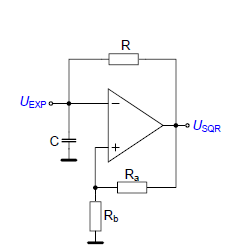
\includegraphics{Obrazky/AE2/2otazka/multivibratorZapojenie}	
		\caption{Zapojenie multivibrátora.}
		\label{fig:multivibratorzapojenie}
	\end{subfigure}
	\begin{subfigure}[b]{0.48\textwidth}
		\centering
		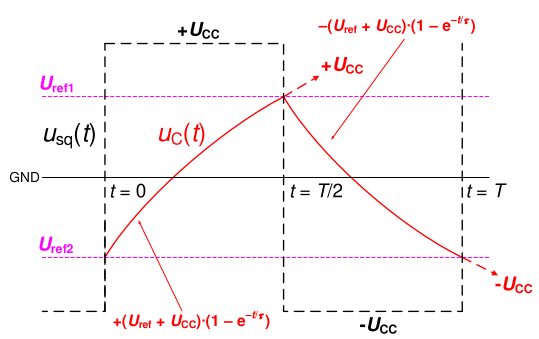
\includegraphics[width=0.7\linewidth]{Obrazky/AE2/2otazka/multivibratorPriebehy}
		\caption{Priebeh napätia v uzloch multivibrátora}
		\label{fig:multivibratorpriebehy}
	\end{subfigure}
\end{figure}
\subsection{Funkčný generátor s bezstratovým integrátorom}
\begin{itemize}
	\item Nahrádza stratový integračný článok bezstratovým integrátorom. $\rightarrow$ Kondík sa nabíja konštantným prúdom $\rightarrow$ výsledok je lineárny nárast napätia na kondenzátore.
	\item Umožňuje získať pílový alebo trojuholníkový priebeh.
	\item Vychádza z relaxačného generátoru, pridáva sa buď invertujúci jednotkový zosilňovač alebo neinvertujúci komparátor.
	\item Je potrebný invertujúci integrátor.
\end{itemize}
\begin{figure}[H]
	\centering
	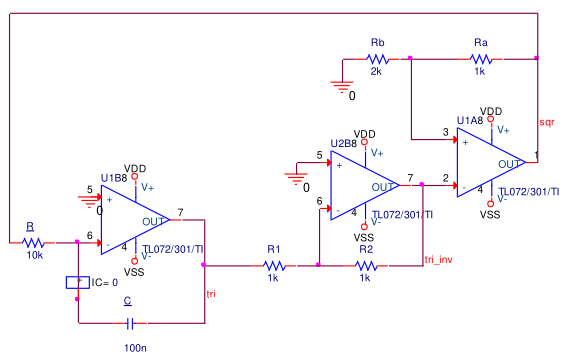
\includegraphics[width=0.45\linewidth]{Obrazky/AE2/2otazka/funkcnyGeneratorZapojenie2}
	\caption{Zapojenie funkčného generátora, s invertujúcim komparátorom}
	\label{fig:funkcnygeneratorzapojenie2}
\end{figure}
\begin{equation}
	T = \frac{1}{f_0} = 4 R C \left(\frac{R_b}{R_a + R_b}\right)
\end{equation}
\begin{figure}[H]
	\begin{subfigure}[b]{0.48\textwidth}
		\centering
		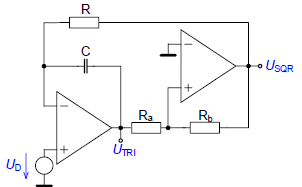
\includegraphics[width=0.7\linewidth]{Obrazky/AE2/2otazka/funkcnyGeneratorZapojenie}
		\caption{Zapojenie funkčného generátora.}
		\label{fig:funkcnygeneratorzapojenie}
	\end{subfigure}
	\begin{subfigure}[b]{0.48\textwidth}
		\centering
		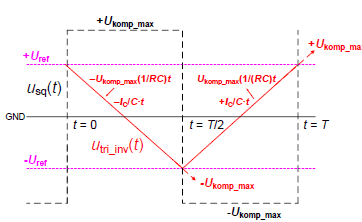
\includegraphics[width=0.7\linewidth]{Obrazky/AE2/2otazka/funkcnyGeneratorPriebehy}
		\caption{Priebehy funkčného generátora s neinvertujúcim komparátorom.}
		\label{fig:funkcnygeneratorpriebehy}
	\end{subfigure}
	\caption{Funkčný generátor s neinvertujúcim komparátorom}
	\label{fig:gen}
\end{figure}
\begin{equation}
	T = \frac{1}{f_0} = 4 R C \left(\frac{R_a}{R_b}\right)
\end{equation}
Pre zapojenie \ref{fig:gen} je možné meniť striedu generátora DC zdrojom napätia. Rovnako je možné využiť iné spôsoby:
\begin{figure}[H]
	\centering
	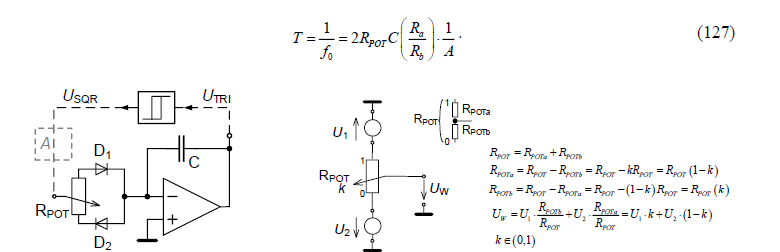
\includegraphics[width=0.8\linewidth]{Obrazky/AE2/2otazka/riadenieGeneratora}
	\caption{Riadenie Striedy a Frekvencie generátora.}
	\label{fig:riadeniegeneratora}
\end{figure}
\begin{itemize}
	\item Strieda sa riadi pomocou potenciometra.
	\item Frekvencia sa riadi pomocou vloženého lineárneho zosilňovača
\end{itemize}
\subsection{Generátor s 555}
\begin{figure}[H]
	\centering
	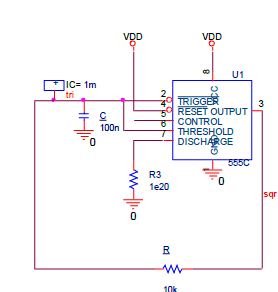
\includegraphics[width=0.35\linewidth]{Obrazky/AE2/2otazka/generator555}
	\caption{Funkčný generátor s časovačom 555 $\rightarrow$ nie je to AKO}
	\label{fig:generator555}
\end{figure}
\begin{itemize}
	\item 555 samé o sebe nedokáže urobiť \qty{50}{\%} striedu
	\item Komparátor je realizovaný spôsobom, kedy je C nabíjané z 555, nie z $U_{CC}$
	\item Využíva sa interného okienkového komparátoru 555.
	\item Oproti AKO sa ušetrí jedna dióda a odpor.
	\item \[T = 2 R C \ln(2)\]
\end{itemize}
\subsection{Generátor s CCII+}
\begin{itemize}
	\item Prúdový konvejor
	\item Využíva sa internej väzby pre komparátor (prúd záporného vstupu = prúd prúdového výstupu)
\end{itemize}
\begin{figure}[H]
	\centering
	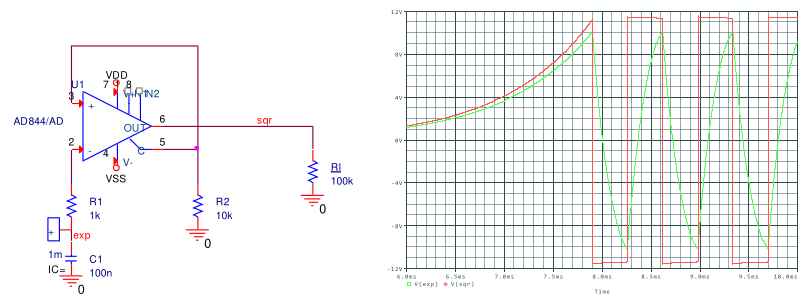
\includegraphics[width=0.7\linewidth]{Obrazky/AE2/2otazka/CCIIgen}
	\caption{Generátor s CCII+ - AD844}
	\label{fig:cciigen}
\end{figure}

\subsection{Generátor OTA}
\begin{itemize}
	\item Jednoduchá aplikácia.
	\item Úsporné riešenie, jedno z najlepších.
	\item Ľahká realizácia bezstratového integrátora, či už invertujúceho alebo neinvertujúceho.
	\item Komparačné hladiny sú $\pm$ maximálne napätie na $R$ v komparátore. Toto sa dá upraviť deličom.
	\subitem Komparátor funguje tak, že pri prebudení OTA, je na výstupe maximálny možný prúd s danou polaritou.
	\item Výhoda je zemnená kapacita.
	\item Dá sa modifikovať tak, že sa to celé riadi zdrojom prúdu.
	\item Bežné moderné riešenie na čipe.
	\item Možnosť zmeny frekvencie aj striedy nezávisle na sebe.
	\item Strieda sa dá ovplyvniť len pridaním zdroja prúdu ku kondenzátoru.
\end{itemize}
\begin{figure}[H]
	\centering
	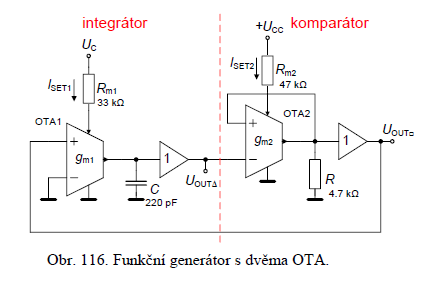
\includegraphics[width=0.7\linewidth]{Obrazky/AE2/2otazka/generatorOTA}
	\caption{Generátor postavený z OTA}
	\label{fig:generatorota}
\end{figure}

\chapter{Operačné zosilňovače, vlastnosti a použitie}
\section{Kmitočtové charakteristiky OZ}
Operačný zosilňovač so spätnou väzbou je uzavretý systém, ktorý je popísaný Blackovým vzťahom $\rightarrow$ teda môže dochádzať k nestabilite. Stabilitu OZ vieme vyšetriť na základe Nyquistovho či Bodeho kritéria stability.
\subsection{Nyquistovo kritérium stability}
\begin{itemize}
	\item Hodograf
	\item Závislosť imaginárnej zložky prenosu $\beta(j\omega)A(j\omega)$ na reálnej zložke.
	\item Systém je stabilný pokiaľ krivka v komplexnej rovine neobopína a ani neprechádza bodom $\left[1,0j\right]$
\end{itemize}
\begin{figure}[H]
	\centering
	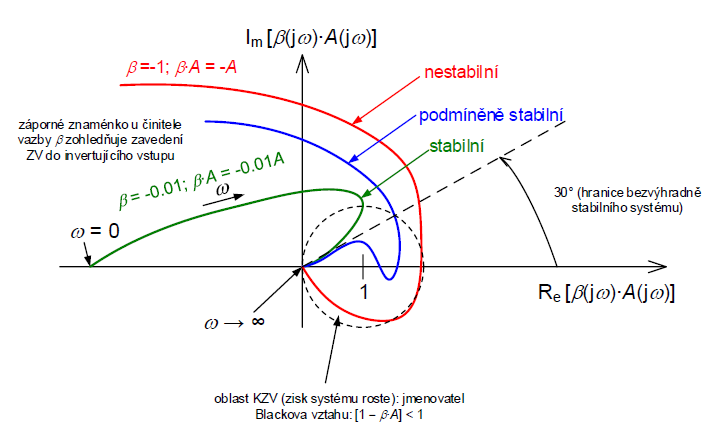
\includegraphics[width=0.7\linewidth]{Obrazky/AE2/3otazka/hodografNyquist}
	\caption{Komplexné zobrazenie Nyquistovej podmienky stability.}
	\label{fig:hodografnyquist}
\end{figure}
\subsection{Bodeho kritérium stability - GM, PM}
Zaoberá sa fázovou a amplitúdovou rezervou ktorá chýba v otvorenej slučke k dosiahnutiu zisku 1 a fázového posuvu \qty{-180}{\degree} $\rightarrow$ teda k dosiahnutiu nestabilného stavu.
\begin{itemize}
	\item Stabilný systém je ak má minimálne fázovú bezpečnosť $\text{PM} >= 45^\circ$
	\subitem V praxi sa zvykne vyžadovať $\text{PM} >= 60^\circ$ $\rightarrow$ zvýšená fázová bezpečnosť postihuje start-up stavy, impulzy a pod.
	\item Čím väčší je menovateľ Blackovho vzťahu $\rightarrow$ tým väčší je zisk systému $\rightarrow$ blíži sa k nestabilite.
	\item Jedno z Bodeho kritérií stability: Prenos celej slučky prechádza frekvenčnou osou v bode 0dB s maximálnym sklonom \qty{-40}{dB/dec} $\rightarrow$ teda ide maximálne o obvod 2. rádu.
	\item Najlepšie je ak sa frekvenčná os pretína so sklonom \qty{-20}{dB/dec}, nakoľko vtedy nedochádza k vzniku oblastí kladnej spätnej väzby a celková odozva je bez rezonančných prevýšení.
	\item \textbf{Bodeho poučka o stabilite:} Systém bude stabilný, ak je rozdiel strmostí charakteristík inverznej spätnej väzby $|1/\beta(j\omega)|$ a zisku zosilňovača $|A(j\omega)|$ v mieste priesečníku $20\text{ dB/dek}$ (najviac $40\text{ dB/dek}$ s dostatočnou rezervou pred ďalším zlomom).
\end{itemize}
\begin{figure}[H]
	\centering
	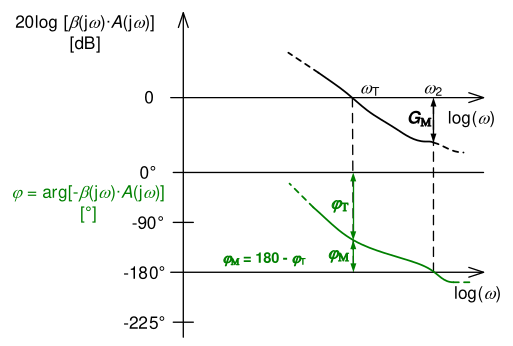
\includegraphics[width=0.6\linewidth]{Obrazky/AE2/3otazka/bodehoDiagram}
	\caption{Bodeho diagram}
	\label{fig:bodehodiagram}
\end{figure}
\begin{figure}[H]
	\centering
	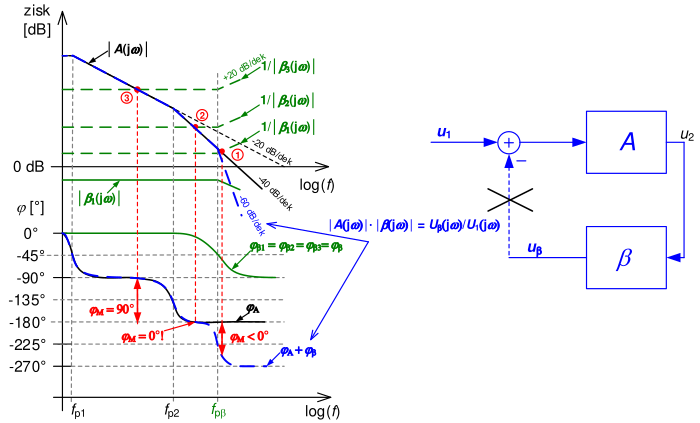
\includegraphics[width=0.7\linewidth]{Obrazky/AE2/3otazka/bodehoDiagramPopis}
	\caption{Frekvenčná charakteristika celého systému pri rozpojenej slučke, dielči prenos zosilňovača a spätnej väzby.}
	\label{fig:bodehodiagrampopis}
\end{figure}
\begin{description}
	\item[Bod č. 1:] Pretína sa tu frekvenčná závislosť $A(j\omega)$ a $\beta_1 (j\omega)$, ale fázová rezerva je menšia ako $0$, preto je obvod nestabilný. Energie a zisku je na to stále dosť (nad $0\text{ dB}$), no neprejaví sa to zrejme priamo osciláciami, ale skôr trvalou saturáciou výstupu, prípadne pri budení signálom preklápaním $\rightarrow$ v tomto stave ide vlastne o "komparátor", pretože má kladnú spätnú väzbu. Podmienka stability v bode č. 1 rozhodne nie je splnená, keďže rozdiel strmostí činí $|1/\beta_1(j\omega)| - |A(j\omega)| = +20\text{ dB/dek} - (-40\text{ dB/dek}) = +60\text{ dB/dek}$.
	
	\item[Bod č. 2:] Nachádzame sa presne na medzi stability (nulová fázová rezerva). Systém opäť pravdepodobne nebude kmitat harmonicky, ale bude v saturácii, pretože zosilnenie je pomerne vysoké. Pre harmonické kmitanie by pri splnení fázovej podmienky muselo byť zosilnenie nižšie, len mierne nad $0\text{ dB}$. Rozdiel strmostí modulov je teraz $+40\text{ dB/dek}$, ale je vidieť, že sa už nachádzame za ďalším zlomom ($f_{p2}$).
	
	\item[Bod č. 3:] Systém je stabilný, pretože fázová bezpečnosť je dostatočne väčšia ako $45^\circ$ a rozdiel strmostí modulov je $+20\text{ dB/dek}$.
\end{description}
\section{Kompenzácia frekvenčnej charakteristiky}
Frekvenčnú charakteristiku vieme kompenzovať:
\begin{itemize}
	\item Odstránením ďalších bodov zlomu $\rightarrow$ pólov nad \qty{0}{\dB}.
	\item Odstránenie zlomu z spätnej väzbe.
\end{itemize}
Popis korekcie:
\begin{itemize}
	\item \textbf{Cieľ korekcie:} Zabezpečiť, aby charakteristika zosilňovania klesala v mieste prechodu cez os $0\text{ dB}$ (jednotkový zisk) miernym sklonom – ideálne len $-20\text{ dB/dek}$ (maximálne $-40\text{ dB/dek}$), čo zaručuje stabilitu.
	
	\item \textbf{Vyrušenie kritického pólu (metóda pól-nula):} Korekčný obvod na vstupe vytvorí v charakteristike tzv. "nulu" ($\tau_a$), ktorú presne naladíme na frekvenciu prvého pólu zosilňovača ($\tau_1$). Táto nula kompletne vymaže (vyruší) pôvodný zlom zosilňovača, takže charakteristika v danom mieste nezačne padať strmšie.
	
	\item \textbf{Vytvorenie nového dominantného pólu:} Korekčný obvod namiesto toho zavedie nový, umelý pól na oveľa nižšej frekvencii ($f_b$). Zisk tak začne klesať oveľa skôr, no kontrolovane a pozvoľna.
	
	\item \textbf{Zníženie jednosmerného (DC) zisku:} Pomocou sériového odporu $R_S$ na vstupe sa zámerne o niečo zníži celkový zisk systému. Tým sa celá frekvenčná charakteristika posunie smerom nadol a tretí (nebezpečný) pól zosilňovača sa dostane bezpečne pod úroveň $0\text{ dB}$, kde už nemôže spôsobiť nestabilitu.
	
	\item \textbf{Alternatíva (Vnútorná kompenzácia):} Okrem externých súčiastok na vstupe (ako $R_k, C_k$) sa stabilita často rieši aj pripojením internej kompenzačnej kapacity priamo do vnútornej tranzistorovej štruktúry operačného zosilňovača.
\end{itemize}
\begin{figure}[H]
	\centering
	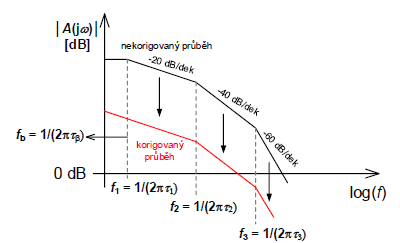
\includegraphics[width=0.55\linewidth]{Obrazky/AE2/3otazka/KorekciaFrekChar}
	\caption{Korekcia frekvenčnej charakteristiky zosilňovača $\rightarrow$ zníženie strmosti prechodu \qty{0}{\dB}.}
	\label{fig:korekciafrekchar}
\end{figure}
\begin{figure}[H]
	\begin{subfigure}[b]{0.48\textwidth}
		\centering
		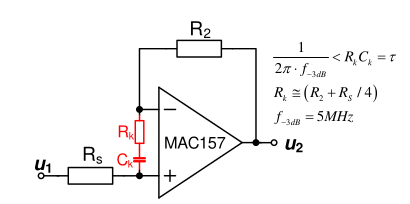
\includegraphics[width=0.7\linewidth]{Obrazky/AE2/3otazka/korekeciaPredOZ}
		\caption{Príklad korekcie pred vstupom do OZ}
		\label{fig:korekeciapredoz}
	\end{subfigure}
	\begin{subfigure}[b]{0.48\textwidth}
		\centering
		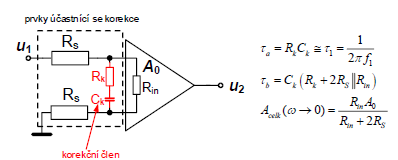
\includegraphics[width=0.7\linewidth]{Obrazky/AE2/3otazka/korekeciaVoVnutriOZ}
		\caption{Príklad korekcie priamo v OZ}
		\label{fig:korekeciavovnutrioz}
	\end{subfigure}
\end{figure}
\section{Kompenzácia kapacitnej záťaže OZ}
\begin{itemize}
	\item Zmiernenie vplyvu kapacitnej záťaže je možné úpravou spätnej väzby ZV.
	\item Parazitná kapacita na výstupe $\rightarrow$ teda aj kapacitná záťaž $\rightarrow$ vzniká kapacitami na DPS, pripojenými káblami BNC, hradlá unipolárov výkonových.
	\item Kapacitu je ťažké definovať, niektoré OZ s ňou počítajú do istej miery.
	\item Vplyvom kapacity vzniká pól s omnoho nižšou frekvenciou ako je tranzientná frekvencia OZ (tranzientná - zisk menej ako 1).
	\item Kapacitná záťaž nemusí nutne znamenať nestabilitu $\rightarrow$ modul sa pretína s \qty{0}{\dB} so strmosťou \qty{-40}{dB/dec}, no fázová bezpečnosť je nízka, čo za istých podmienok môže vyvolať nestabilitu.
	\item Riešenie spočíva v pridaní korekčnej kapacity do spätnej väzby $\rightarrow$ toto môže zvýšiť fázovú bezpečnosť až do \qty{60}{\degree}.
	\item Nutné zvoliť optimálnu hodnotu.
	\subitem Malá hodnota $\rightarrow$ stále nestabilné.
	\subitem Veľká hodnota $\rightarrow$ zase nestabilné.
	\subitem Treba voliť stred.
\end{itemize}
\begin{figure}[H]
	\centering
	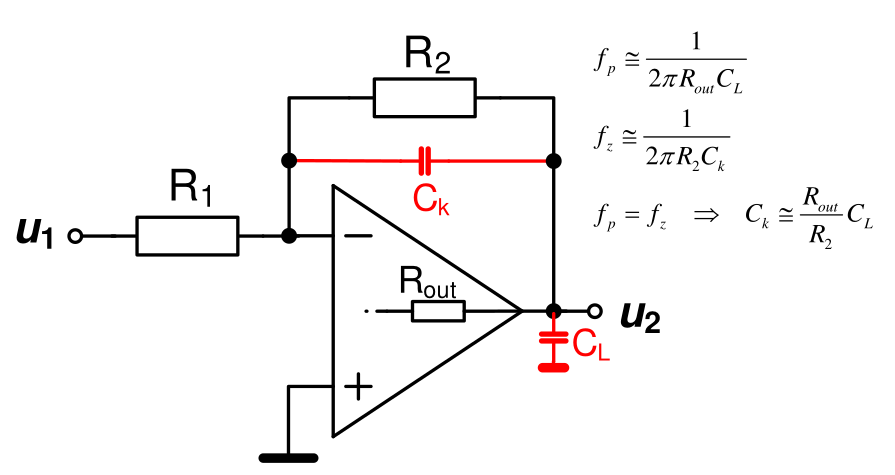
\includegraphics[width=0.5\linewidth]{Obrazky/AE2/3otazka/korekcnaKapacitaVZV}
	\caption{Korekčná kapacita v spätnej väzbe.}
	\label{fig:korekcnakapacitavzv}
\end{figure}
\section{Obmedzenie rýchlosti prebehu $\rightarrow$ Slew Rate}
Rýchlosť prebehu definuje najrýchlejšie zmeny ktoré je zariadenie schopné spracovať s ohľadom na zmenu vstupného signálu. Jej konečná rýchlosť súvisí s nelineárnym skreslením $\rightarrow$ dôvodom existencie skreslenia a aj konečnej rýchlosti prebehu je obmedzenie výstupného prúdu diferenčného stupňa zosilňovača, resp. iných častí obvodu.
\begin{figure}[H]
	\centering
	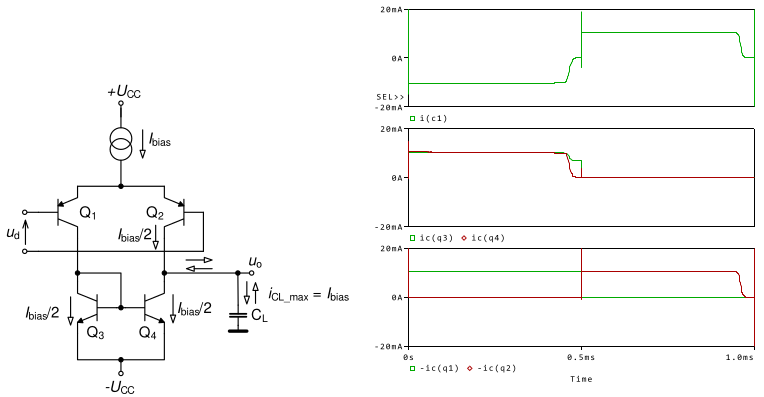
\includegraphics[width=0.55\linewidth]{Obrazky/AE2/3otazka/SRzrkadlo}
	\caption{Diferenčný stupeň so zrkadlom a kapacitnou záťažou.}
	\label{fig:srzrkadlo}
\end{figure}
\begin{description}
	\item[Extrém A] Prebudený vstup uzavrie T1 $\rightarrow$ prúdové zrkadlo nepracuje $\rightarrow$ celý $I_{bias}$ tečie cez T2 a nabíja kapacitu $C_L$
	\item[Extrém B] Opačne prebudený vstup uzavrie T2 $\rightarrow$ $I_{bias}$ tečie cez T1, to otvára prúdové zrkadlo, ktoré vybíja kapacitu $C_L$
\end{description}
\begin{itemize}
	\item Rýchlosť prebehu je obmedzená javmi pri nabíjaní kapacít spôsobenými obmedzením náboja na kapacite. Maximálny nárast náboja je obmedzený.
	\item SR je obmedzené najväčšou možnou zmenou napätia na $C$ za čas, spôsobené maximálnym prúdom ktorý $C$ nabíja
	\item DEF: SR je maximálna zmena výstupného napätia za čas.
	\item \begin{equation}
		SR \approx \frac{\Delta U_0}{\Delta t} = \frac{I_{bias}}{C_L}
	\end{equation}
	\item Ovplyvňujú ho aj kapacity v záťaži obvodu.
	\item SR je definované uzlom ktorý má najmenší pomer $\frac{I_{bias}}{C_L}$.
	\item Skreslenie SR sa zamedzí ak: \begin{equation}
		f_{max} = \frac{SR}{2\pi U_{out}}
	\end{equation}
	\item Skreslenie sa prejavuje tak, že pri harmonickom vstupnom signále sa na výstup dostavuje trojuholník $\rightarrow$ toto je extrémny prípad.
	\item Voči SR sa nedá bojovať zápornou spätnou väzbou $\rightarrow$ nakoľko tá by len vrátila skreslený signál na vstup.
\end{itemize}
\section{Šumy v OZ}
\begin{itemize}
	\item Šum ako taký má náhodný charakter a je definovaný gaussovským rozložením pravdepodobnosti.
	\item Je definovaný v čase aj v šírke pásma
	\item \textbf{Trochu symboliky:}
	
	\begin{description}
		\item[$u_N(t)$] - hodnota k $1\text{ Hz}$ (efektívna hodnota šumu = smerodajná odchýlka), v podstate efektívna hodnota šumu v pásme $1\text{ Hz}$.
		\item[$U_N(t)$] - hodnota ku konkrétnej šírke pásma.
		\item[$u_{\text{noise}}(t)$] – okamžité napätie šumu.
		\item[$u_N^2(t)$] - "stredný" šumový výkon (na odpore $1\ \Omega$).
	\end{description}
\end{itemize}
\begin{figure}[H]
	\centering
	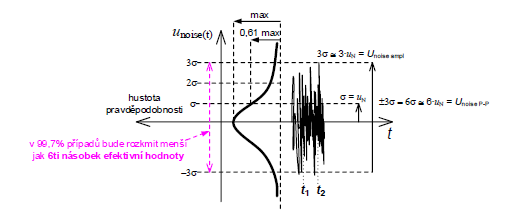
\includegraphics[width=0.7\linewidth]{Obrazky/AE2/3otazka/sumVOZ}
	\caption{Náhodný charakter šumu, výstrelový a biely, jeho statický popis}
	\label{fig:sumvoz}
\end{figure}
Stredná hodnota šumu:
% Stredná kvadratická hodnota šumu
$$u_N^2 = \overline{u_N^2} = \frac{1}{t_2 - t_1} \int_{t_1}^{t_2} u_{\text{noise}}^2(t) \, \text{d}t$$

% Efektívna hodnota šumu
Efektívna hodnota šumu:
$$u_N = \sqrt{\frac{1}{t_2 - t_1} \int_{t_1}^{t_2} u_{\text{noise}}^2(t) \, \text{d}t}$$

% Šumová výkonová a prúdová hustota
Výkonové hodnoty šumu:
$$u_N^2 = \frac{U_N^2}{B} \left[ \frac{\text{V}^2}{\text{Hz}} \right] ; \quad i_N^2 = \frac{I_N^2}{B} \left[ \frac{\text{A}^2}{\text{Hz}} \right]$$

% Spektrálna hustota šumového napätia
Spektrálna hustota šumu:
$$u_N = \frac{U_N}{\sqrt{B}} \left[ \frac{\text{V}}{\sqrt{\text{Hz}}} \right]$$

\begin{figure}[H]
	\centering
	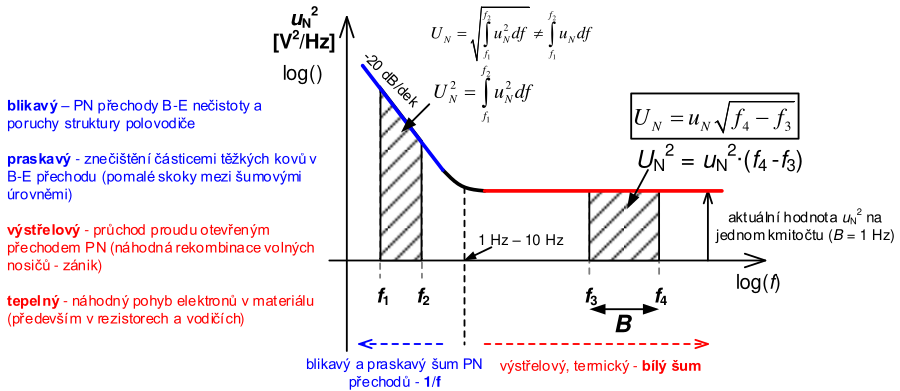
\includegraphics[width=0.7\linewidth]{Obrazky/AE2/3otazka/vykonovaSpektralnaHustotaZdrojeSumu}
	\caption{Výkonová spektrálna hustota a zdroje šumov v obvode.}
	\label{fig:vykonovaspektralnahustotazdrojesumu}
\end{figure}

Šumové pásmo sa rozdeľuje na oblasť pomalých dejov $\frac{1}{f}$, a oblasť bieleho $\rightarrow$ výstrelového šumu.
Výkon šumu závisí na šírke pásma, pričom celková šírka pásma nie je rovná šírke pásma pre pokles o \qty{-3}{\dB}, ale počíta sa z rovností plôch pod ideálnou obdĺžnikovou frekvenčnou charakteristikou:
\begin{equation}
	B_N = \frac{1}{\left|K_{max}\right|} \int_{0}^{\infty} \left|K(f)\right| \,df
\end{equation}
Zdroje šumu sa dajú zrátať dokopy len prostredníctvom výkonu $\rightarrow$ nakoľko majú náhodný charakter, nie sú korelované, nemajú orientáciu.
\begin{figure}[H]
	\centering
	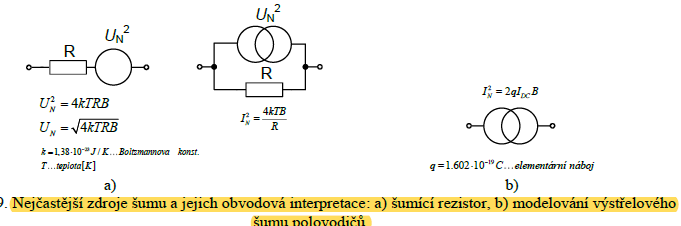
\includegraphics[width=0.7\linewidth]{Obrazky/AE2/3otazka/zdrojeSumuVobvode}
	\caption{Zdroje šumu v obvodoch pre modelovanie}
	\label{fig:zdrojesumuvobvode}
\end{figure}
Šumy v rámci OZ:
\begin{itemize}
	\item V rámci OZ existuje mnoho zdrojov šumu $\rightarrow$ všetky sa uvažujú naraz na výstupe.
	\item Pre zníženie šumu je výhodné používať nízkoimpedančné zdroje signálu $\rightarrow$ veľký odpor má veľký tepelný šum, pričom prevádza prúdové šumy zo vstupu OZ na napätie.
	\item OZ s unipolárnym vstupným párom má nižšie úrovne šumu
	\item Pre nižší šum je vhodné používať čo najmenej rezistorov.
	\item Šumové vlastnosti dvojbranu sú definované šumovým číslom $NF$ (noise figure) v [dB].
	\subitem Toto číslo definuje koľkokrát sa zmenší SNR na vstupe OZ oproti SNR na výstupe OZ.
	\item \begin{equation}
		NF = 20 \log \left[\frac{\frac{U_{sig}}{U_{noise}}\text{in}}{\frac{U_{sig}}{U_{noise}}\text{out}}\right]
	\end{equation}
	\item V kaskádneho radenia existuje Freesov vzťah:
	\item \begin{equation}
		F = F_1 + \frac{F_2 -  1}{A_1} + \frac{F_3 - 1}{A_1 A_2} + \dots + \frac{F_n - 1}{\prod_{i=1}^{n-1} A_{i}}
	\end{equation}
	\item Kedy najväčšie zosilnenie a najväčšie šumové číslo sa umiestňuje do prvého miesta v kaskáde $\rightarrow$ zvyšok má menší vplyv.
\end{itemize}
Ďalšie zdroje šumu:
\begin{itemize}
	\item Parazitné kapacity $\rightarrow$ dá sa potlačiť tienením a usporiadaním
	\item Parazitné induktívne väzby $\rightarrow$ dá sa potlačiť zmenšením rozmerov, skrátením prívodov, zväčšením zemnej plochy
	\item Iskrenie relé a kontaktov v ňom 
	\item Termoeletrické napätia a impulzné špičky $\rightarrow$ dá sa potlačiť teplotnou stabilitou
\end{itemize}
\begin{figure}[H]
	\centering
	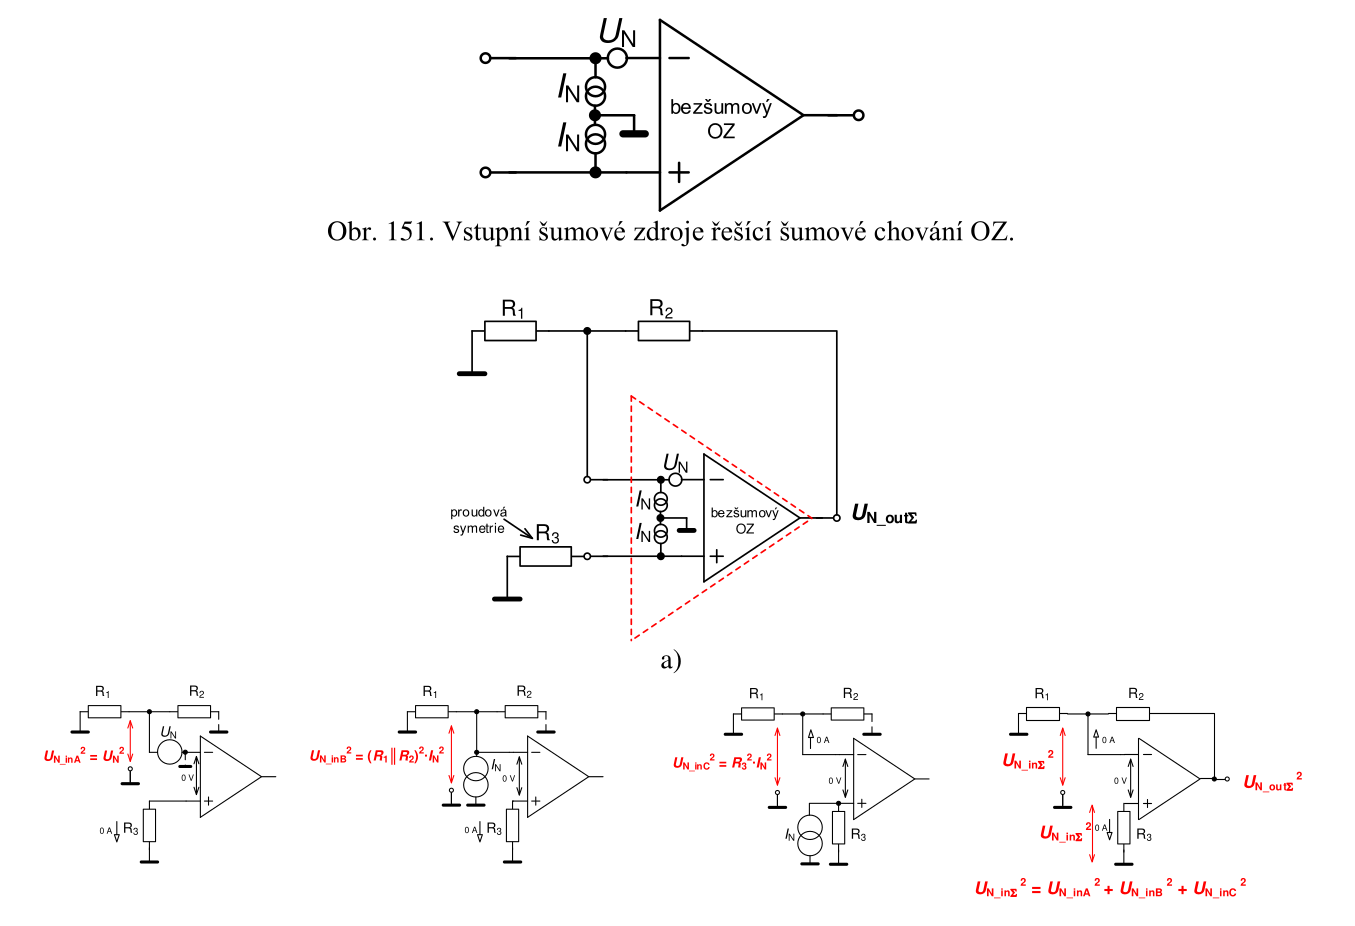
\includegraphics[width=0.9\linewidth]{Obrazky/AE2/3otazka/sumyVoz}
	\caption{Šumová analýza OZ}
	\label{fig:sumyvoz}
\end{figure}
\section{Statická elektrika $\rightarrow$ ochrana proti ESD}
\begin{itemize}
	\item Problémy s ESD vznikajú pri trení povrchov predmetov a plôch.
	\item Pri výboji ESD dochádza k extrémne krátkemu výboju o prúde niekoľko ampér, nanosekundy, s napätiami až niekoľko kV $\rightarrow$ toto nám zabije operák
	\item OZ a integrované obvody obsahujú integrovanú ochranu voči ESD priamo od výrobcov.
	\begin{itemize}
		\item Primárna ochrana
		\subitem Clampy so sériovými rezistormi $\rightarrow$ obmedzenie výbojových prúdov
		\item Sekundárna ochrana
		\subitem Rezistory a clampy chrániace pred vlastnou funkčnou tranzistorovou štruktúrou
		\subitem V prípade, že ochrany nie sú dostatočne rýchle môže sa použiť iný ochranný prvok v rámci silikónu $\rightarrow$ \emph{ESDCGNMOS}.
		\subitem Vysoké hodnoty ochranných rezistorov spôsobujú šum, preto sa rozdeľujú veľké hodnoty do niekoľkých menších hodnôt.
		\subitem Pri rýchlych RF obvodoch sa však požiadavky na ESD zrážajú s požiadavkami na rýchlosť a šírku pásma $\rightarrow$ je nutný kompromis.
	\end{itemize}
	\item Odolnosť MOSFET súčiastok je voči ESD menšia ako JFET a BJT
\end{itemize}
Zásady pri práci s ESD citlivými súčiastkami:
\begin{itemize}
	\item Prepravovať vo fixnom nevodivom prostredí, ideálne so skratovanými vývodmi.
	\item Nechytať sa vývovod.
	\item Pracovný odev bez syntetických vlákien.
	\item Uzemniť sa.
\end{itemize}
\begin{figure}[H]
	\centering
	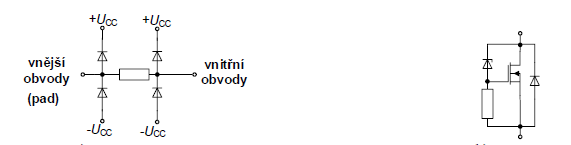
\includegraphics[width=0.7\linewidth]{Obrazky/AE2/3otazka/ochranaESD}
	\caption{Primárna Clamp ochrana a rýchly ESDCGNMOS.}
	\label{fig:ochranaesd}
\end{figure}
\section{Ochrana vstupov, výstupov a napájania OZ voči prepólovaniu, a skratom}
\begin{itemize}
	\item Jedná sa o ochranu pred nedovolenou napäťovou úrovňou, obmedzenie výstupného prúdu
	\item Ochrana voči prepólovaniu: Zapojenie ochranných diód do série s napájaním.
	\item Ochrana vstupov so štandardnou spätnou väzbou $\rightarrow$ antiparalelné zapojenie diód $\rightarrow$ diferenčné napätie.
	\item Používajú sa rýchle spínacie diódy $\rightarrow$ diódy delinearizujú vstupný odpor a nesmú reagovať až príliš
	\item V prípade, že zosilňovač pláva $\rightarrow$ je nutné zaistiť ochranu voči common-mode napätí.
	\subitem Zhoršenie vstupného odporu a common mode rejection ratio.
	\subitem Zhoršenie je dané kvalitou diód.
\end{itemize}
\begin{figure}[H]
	\centering
	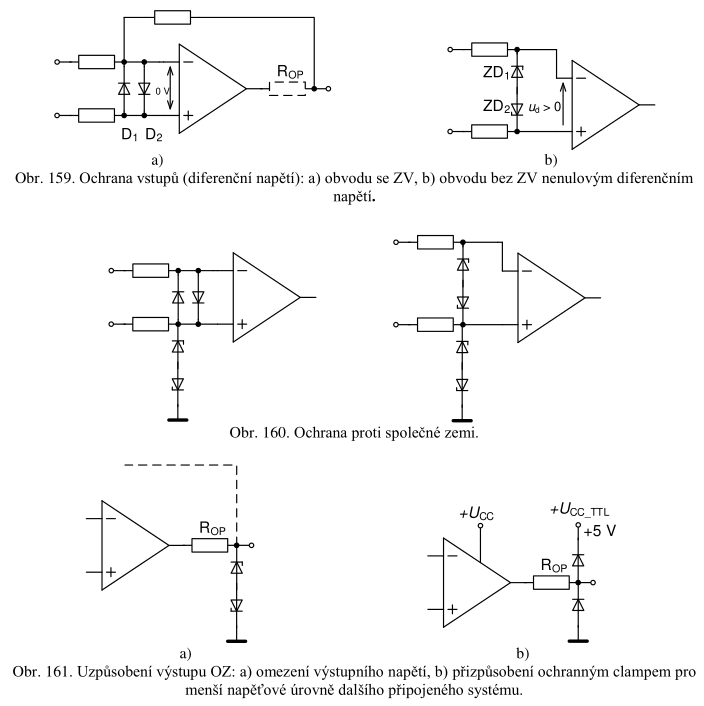
\includegraphics[width=0.7\linewidth]{Obrazky/AE2/3otazka/ochranaVstupov}
	\caption{}
	\label{fig:ochranavstupov}
\end{figure}
\section{Napájanie OZ}
\begin{itemize}
	\item Väčšina OZ vyžaduje a aj má symetrické napájanie
	\subitem V prípade, že nie je dostupné symetrické napájanie $\rightarrow$ vytvorí sa umelá zem v polovičke napájacej hladiny $\rightarrow$ toto môže znamenať problém, nakoľko zem môže plávať s teplotou ak je vytvorená deličom a pod.
	\subitem Vytvára sa z deliča alebo z presných referenčných zdrojov $\rightarrow$ zennerových diód.
	\begin{figure}[H]
		\centering
		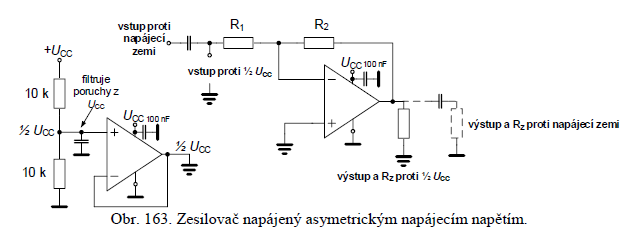
\includegraphics[width=0.7\linewidth]{Obrazky/AE2/3otazka/umelaZem}
		\caption{Umelá zem.}
		\label{fig:umelazem}
	\end{figure}
	\subitem Je potrebné použiť napäťový sledovač $\rightarrow$ pri použití čisto analógovej zeme je obvod po istú dobu po zapnutí nefunkčný, treba OZ.
	\item Dôležitým je správne usporiadanie napájania a zemí $\rightarrow$ najväčší konštrukčný problém.
	\item Napájacia vetva musí mať ideálne nulovú impedanciu $\rightarrow$
	\subitem Inak sa objavujú vplyvy šumu, kmitanie, citlivosť na zmeny v napájacom napätí
	\item Citlivosť na zmeny v napájacom napätí $\rightarrow$ PSRR $\rightarrow$ Power Supply Rejection Ratio
	\subitem Klesá so zvyšujúcou sa frekvenciou
	\subitem Vďaka tomu sa z napájania môže dostať do obvodu VF rušenie pochádzajúce zo zdroja
	\item Obrana voči šumu z napájania $\rightarrow$ blokovací kondenzátor.
	\subitem Pri krátkodobých nárastoch odberu prúdu poskytuje potrebnú energiu.
	\subitem Pracuje aj ako filtre pre VF zložky, ktoré skratuje na zem.
	\subitem Ideálne keramický kondík $\rightarrow$ má nižšie indukčnosti.
	\item Pri použití blokovacích kondenzátorov sa vytvára induktívna slučka vďaka prúdu ktorý tečie z kondíka do obvodu.
	\subitem Pre zamedzenie induktívnych slučiek je potrebné skrátiť vzdialenosti medzi kondíkom, napájaním, zemou a zariadením.
	\begin{figure}[H]
		\centering
		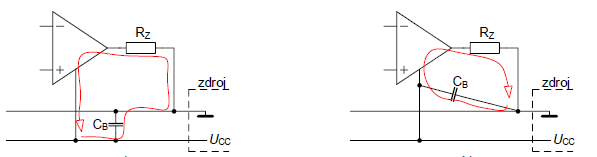
\includegraphics[width=0.7\linewidth]{Obrazky/AE2/3otazka/kondikKratka}
		\caption{Skrátenie induktívnej slučky.}
		\label{fig:kondikkratka}
	\end{figure}
	\item Zemnenie je ďalší problém
	\subitem Zem musí mať zanedbateľnú indukčnosť a čo najmenší odpor
	\subitem Realizuje sa zemniaca plocha pre všeobecnú zem
	\subitem V prípade, že sa uzatvárajú veľké prúdy zemou $\rightarrow$ je potrebné viesť cesty zvlášť $\rightarrow$ rušenie.
	\subitem Ideálna zem neexistuje $\rightarrow$ záleží na veľkosti prúdov
	\subitem Môže dochádzať aj k vytvoreniu kladnej ZV $\rightarrow$ oddelenie zemí a spojenie v inom mieste $\rightarrow$ iná cesta pre signál a pre prúdy.
	\begin{figure}[H]
		\centering
		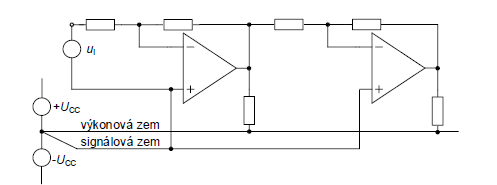
\includegraphics[width=0.7\linewidth]{Obrazky/AE2/3otazka/umelaZem1}
		\caption{Rozdelenie zemí}
		\label{fig:umelazem1}
	\end{figure}
	\item Skurvená parazitná kapacita vstupu voči zemi:
	\subitem Môže spôsobiť nárast zosilnenia na vysokých frekvenciách $\rightarrow$ vytvára parazitný pól
	\subitem Vysoké prevýšenie zisku $\rightarrow$ tvorí oscilácie $\rightarrow$ kompenzačná kapacita a tlmenie činiteľa akosti pomocou odporu
	\begin{figure}[H]
		\centering
		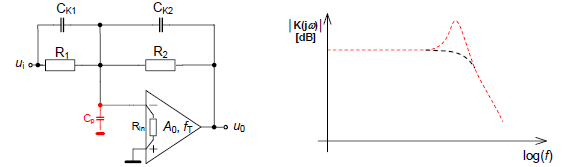
\includegraphics[width=0.7\linewidth]{Obrazky/AE2/3otazka/umelaZem2}
		\caption{Parazitná kapacita na vstupe}
		\label{fig:umelazem2}
	\end{figure}
	
\end{itemize}\section{Diferenčný pár}
\section{Millerov OZ}

\section{Kompenzácia napäťovej a prúdovej nesymetrie OZ}
\begin{itemize}
	\item Reálne OZ sú do istej miery nesymetrické
	\item Majú z výroby prirodzený offset $\rightarrow$ dá sa zistiť pri skratovaní výstupov a meraní napätia na výstupe
	\item Kompenzuje sa privedením opačného napätia na vstup $\rightarrow$ vytvorí sa umelý offset, ktorý kompenzuje ten prirodzený.
	\item Offset je v mV až uV.
	\item Pokiaľ má OZ veľké zosilnenie tak už malý vstupný offset môže saturovať výstup $\rightarrow$ spôsobiť veľkú DC zložku na výstupe
	\item offsetové napätie záleží na teplote $\rightarrow$ teplotný drift súčiastok / offsetu
	\subitem vstupný offset je možné trimmovať laserom pri výrobe
	\begin{figure}[H]
		\centering
		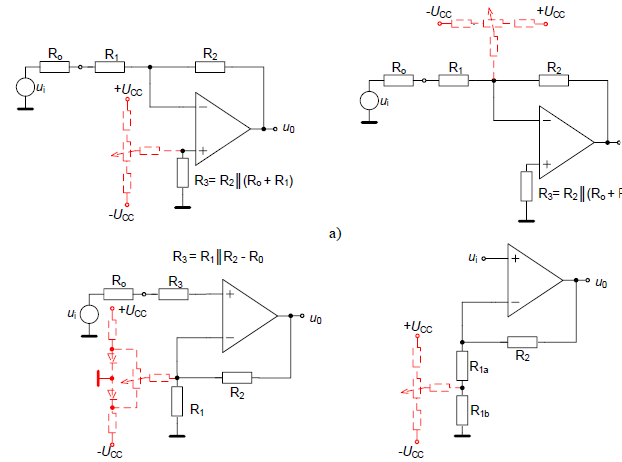
\includegraphics[width=0.5\linewidth]{Obrazky/AE2/3otazka/offsetNapatieKompenzacia}
		\caption{Kompenzácia vstupnej napäťovej nesymetrie.}
		\label{fig:offsetnapatiekompenzacia}
	\end{figure}
	\item Prúdová nesymetria vzniká tým, že OZ má malý vstupný prúd, ktorý je každý iný.
	\item Ich nerovnosti môžu vyvolať rozdiel vstupných napätí
	\item Rieši sa pripojením rezistorov na vstup
	\item Odporové deliče regulujú vstupný prúd inverujúcou a neinvertujúcou vetvou $\rightarrow$ vyrovnávanie prúdov.
\end{itemize}

\section{Diferenčný pár}

\begin{itemize}
	\item Základný stavebný blok OZ.
	\item Prevodník z diferenciálneho vstupného napätia výstupný rozdielový prúd
	\item Je vysoko nelineárny
	\item Existuje bipolárny a unipolárny diferenčný pár.
	\item Tvorí základ pre diferenciálny napäťový zosilňovač
\end{itemize}
\begin{figure}[H]
	\centering
	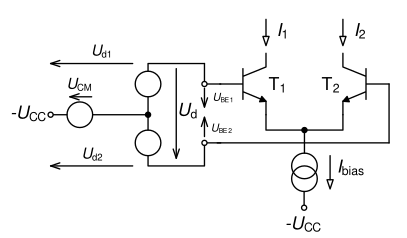
\includegraphics[width=0.5\linewidth]{Obrazky/AE2/3otazka/differ}
	\caption{Bipolárny diferenciálny stupeň pre nelineárnu (veľko signálovú) analýzu.}
	\label{fig:differ}
\end{figure}
Výsledný rozdielový prúd sa dá stanoviť ako:
\begin{equation}
	\Delta I_{out} = I_1 - I_2 = I_{bias}\tanh \left(\frac{U_d}{2U_{TE}}\right)
\end{equation}
Závislosť je jasne nelineárna, v prípade, že $U_d$ je v rozmedzí $\pm 50 \text{ mV}$ môžeme tú závislosť za lineárnu považovať.
\begin{figure}[H]
	\centering
	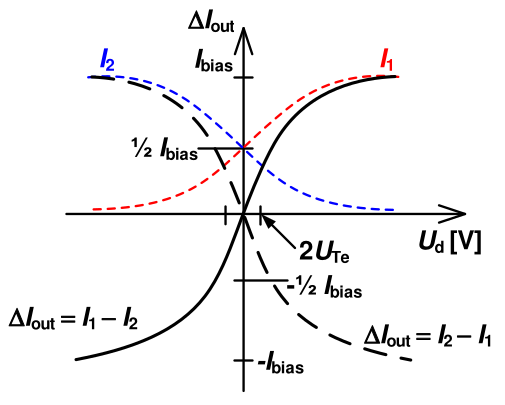
\includegraphics[width=0.3\linewidth]{Obrazky/AE2/3otazka/differZavislost}
	\caption{Prevodová charakterisitka diferenciálneho stupňa.}
	\label{fig:differzavislost}
\end{figure}
\begin{figure}[H]
	\centering
	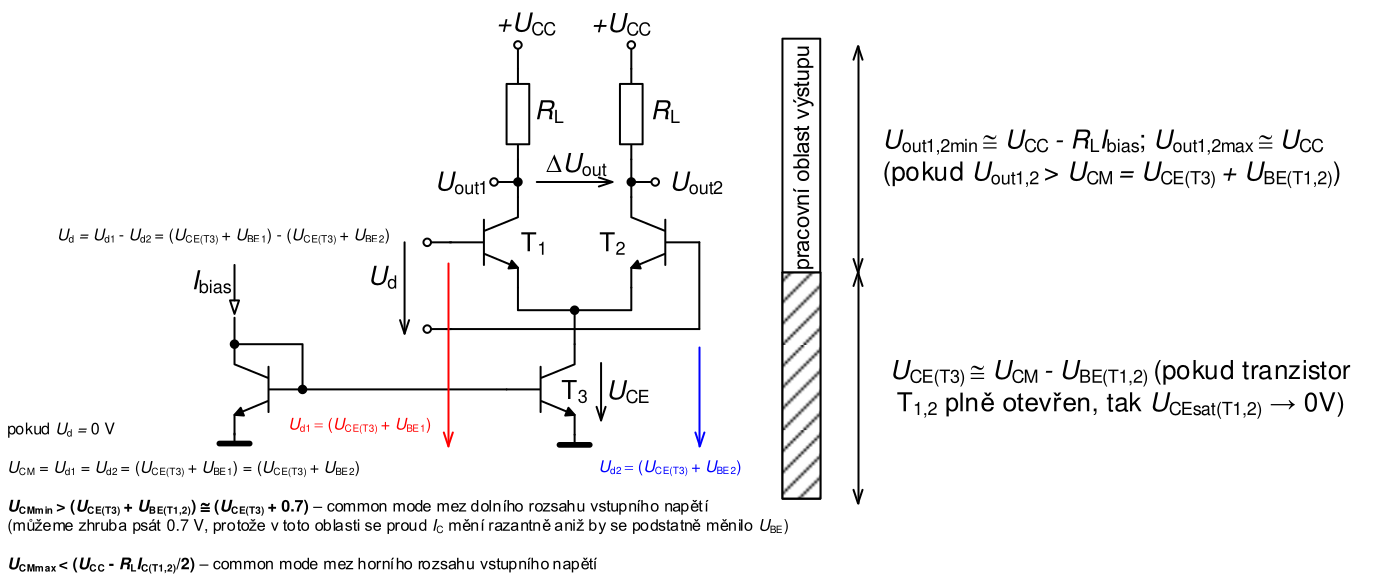
\includegraphics[width=0.75\linewidth]{Obrazky/AE2/3otazka/differZosilnovacSRezZatazou}
	\caption{Diferenčný zosilňovač s rezistívnou záťažou.}
	\label{fig:differzosilnovacsrezzatazou}
\end{figure}
\begin{figure}[H]
	\centering
	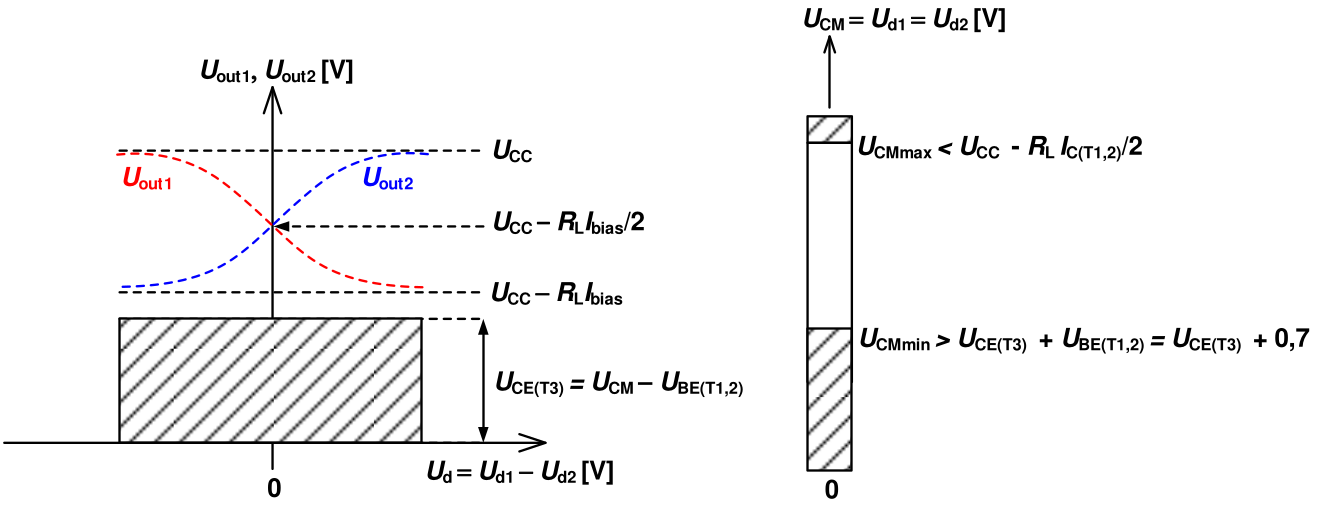
\includegraphics[width=0.7\linewidth]{Obrazky/AE2/3otazka/medzeVstupnychNapatiDiffer}
	\caption{Medze vstupných napätí zosilňovača pre súhlasné napätie vstupov. Statická prevodná charakteristika, medze súhlasného vstupného napätia.}
	\label{fig:medzevstupnychnapatidiffer}
\end{figure}
\begin{figure}[H]
	\centering
	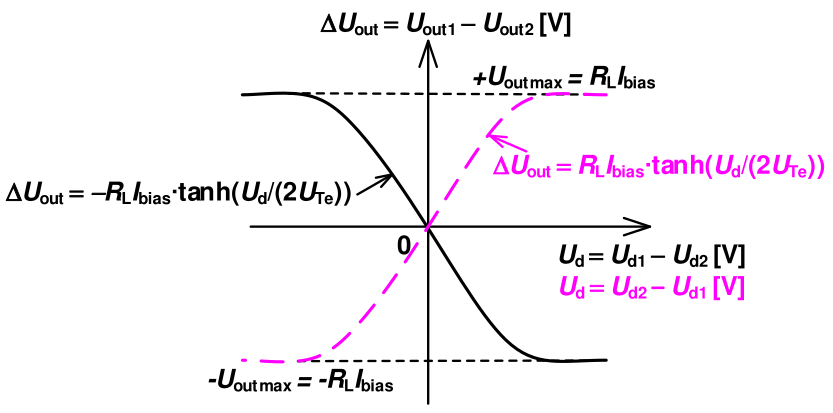
\includegraphics[width=0.4\linewidth]{Obrazky/AE2/3otazka/prevodnaCharakteristikaDiffer}
	\caption{Napäťová prevodná charakteristika.}
	\label{fig:prevodnacharakteristikadiffer}
\end{figure}
\textbf{Diferenciálny zosilňovač je možné linearizovať využitím emitorových degradačných rezistorov.}
\begin{figure}[H]
	\centering
	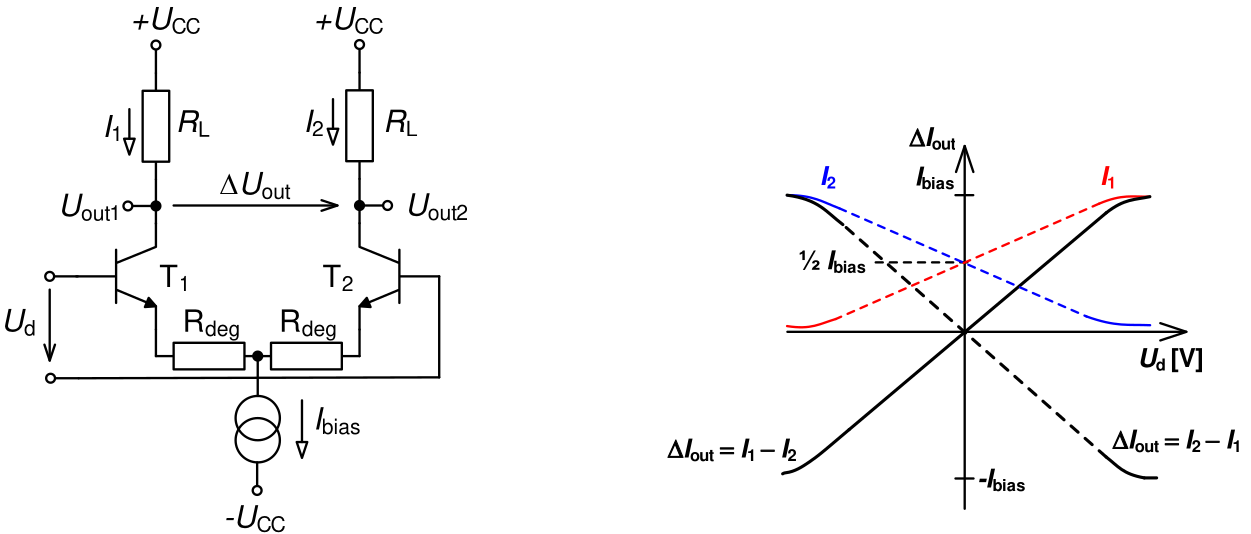
\includegraphics[width=0.7\linewidth]{Obrazky/AE2/3otazka/linearizaciaDiffZosikaVar1}
	\caption{Emitorová degradácia diferenčného zosilňovača.}
	\label{fig:linearizaciadiffzosikavar1}
\end{figure}
\begin{figure}[H]
	\centering
	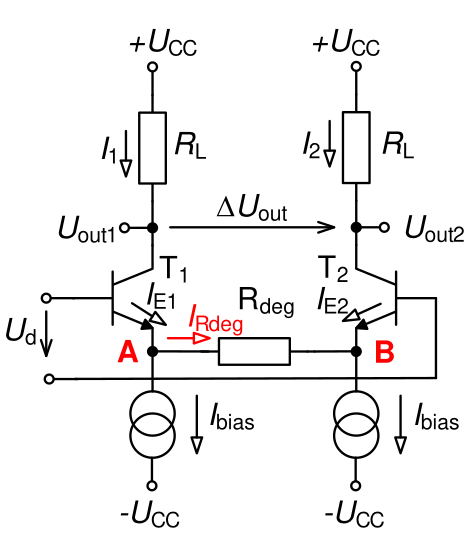
\includegraphics[width=0.3\linewidth]{Obrazky/AE2/3otazka/linearizaciaDiffZosikaVar2}
	\caption{Druhá možnosť emitorovej degradácie diferenčného zosilňovača.}
	\label{fig:linearizaciadiffzosikavar2}
\end{figure}
Ďalej je možná linearizácia pomocou inverznej prevodnej charakteristiky.
\begin{figure}[H]
	\centering
	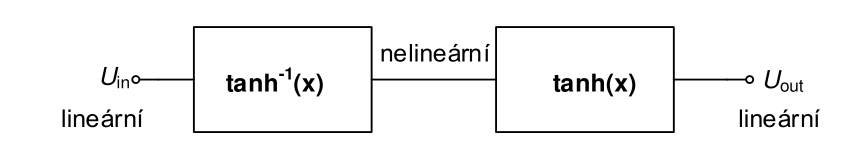
\includegraphics[width=0.35\linewidth]{Obrazky/AE2/3otazka/principLinearizacieInverznouCharakteritikou}
	\caption{Princíp linearizácie pomocou inverznej prevodovej charakteristiky.}
	\label{fig:principlinearizacieinverznoucharakteritikou}
\end{figure}
\begin{figure}[H]
	\centering
	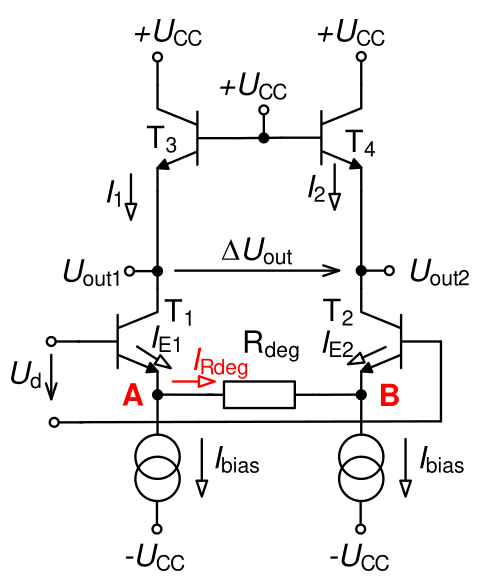
\includegraphics[width=0.3\linewidth]{Obrazky/AE2/3otazka/linearizaciaDiffZosikaVar3}
	\caption{Linearizácia diferenčného zosilňovača s členom funkcie $\tanh^{-1}$}
	\label{fig:linearizaciadiffzosikavar3}
\end{figure}
V praxi sa asi využíva viacero linearizačných techník pre vstup a výstup:
\begin{figure}[H]
	\centering
	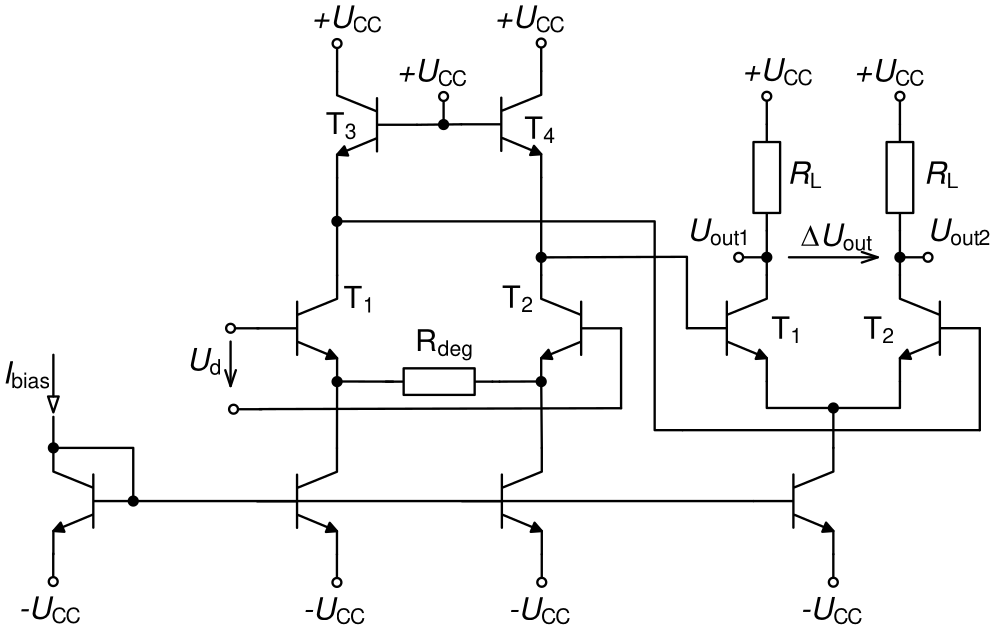
\includegraphics[width=0.7\linewidth]{Obrazky/AE2/3otazka/kompletnaLinearizaciaZosika}
	\caption{Linearizácia diferenčného zosilňovača.}
	\label{fig:kompletnalinearizaciazosika}
\end{figure}
\subsection{Unipolárny diferenciálny pár}
Rovnako ako pre bipolár, je možné skonštruovať aj unipolárnu variantu, závislosť výstupného prúdu je však kvadratická vďaka použitej technológií.
\begin{figure}[H]
	\centering
	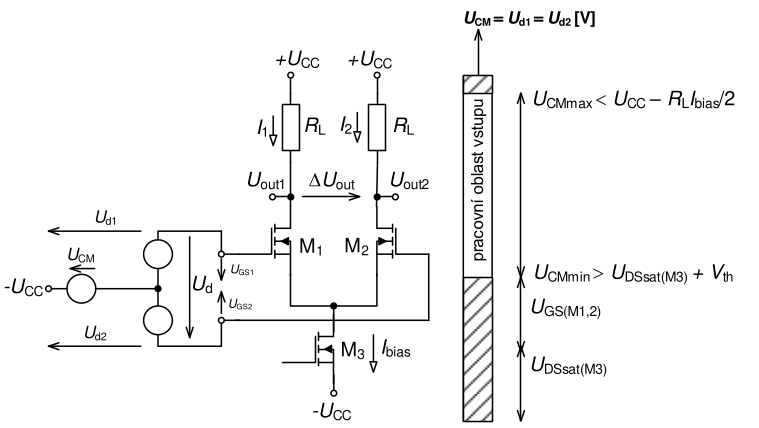
\includegraphics[width=0.7\linewidth]{Obrazky/AE2/3otazka/unipolarLin}
	\caption{Diferenčný zosilňovač s unipolárnym diferenčným párom.}
	\label{fig:unipolarlin}
\end{figure}
Platí, že \begin{equation}
	\Delta i_{out} = \Delta u_d \sqrt{\mu_0 C_{OX} \frac{W}{L} I_{bias}} = \Delta u_d g_m
\end{equation}
\newpage
\section{Millerov OZ}
\begin{itemize}
	\item Má koncový stupeň v triede A
	\item Má niekoľko pólov frekvenčnej charakteristiky $\rightarrow$ sú definované kapacitami vysokoimpedančných uzlov
	\item Bez zásahu nie je žiaden z týchto pólov dominantný na nízkych frekvenciách $\rightarrow$ teda je nestabilný
	\item Stabilita je daná Millerovou kompenzačnou kapacitou v spätnej väzbe $C_M$
	\item Využíva millerovho javu $\rightarrow$ pokiaľ je zapojená v spätnej väzbe tak je transformovaná na ekvivalentnú kapacitu ktorej hodnota už odpovedá kapacite pôvodnej $C_M$ ktorá je zosilnená o stupeň $M_5$
	\item Tranzientná frekvencia je daná zhruba tou kapacitou millerovho javu: \[\text{GBW} = f_{d1} A_U\]
	\item $C_M$ samá o sebe tvorí aj nulu v prenose, tá nám tú stabilitu ešte viac dojebáva, šak prečo nie $\rightarrow$ preto sa vkladá do série odpor $R_M$ s $C_M$ a nula magicky zmizne (boha toto sú kokotiny)
	\item Výstupné napätie na prázdno sa bude nachádzať medzi napájacími limitmi zníženými o saturačné úbytky na výstupných tranzistoroch
\end{itemize}
\begin{figure}[H]
	\centering
	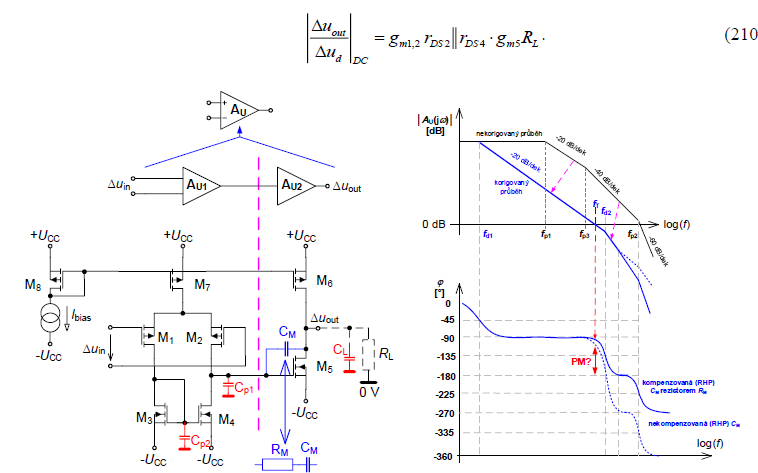
\includegraphics[width=0.7\linewidth]{Obrazky/AE2/3otazka/miller}
	\caption{Millerov dvojstupňový zosilňovač.}
	\label{fig:miller}
\end{figure}

	% !TeX spellcheck = sk_SK-Slovak
% !TeX root = statnicaEKT.tex
\graphicspath{{./Obrazky/SI1/}}   % priečinok s obrázkami (uprav podľa svojej štruktúry v Overleafe)

% ============================================================
\part{BPC-SI1 - Signály 1}
\begin{huge}
	Otázky:
	\newline
\end{huge}
\begin{enumerate}
	\item Otázka - Periodické, kvaziperiodické a neperiodické signály; výpočet výkonu; výpočet spektra; typické príklady.
	\item Otázka - Prevody medzi analógovými a digitálnymi signálmi; vzorkovanie, aliasing; rovnomerné a nerovnomerné kvantovanie; kvantovací šum.
	\item Otázka - Lineárne a nelineárne systémy; vplyv nelinearity na spektrum; stabilné, kauzálne a časovo invariantné systémy; testovací signály.
\end{enumerate}
\newpage

% ============================================================
\chapter{Periodické, kvaziperiodické a neperiodické signály;
výpočet výkonu; výpočet spektra; typické príklady}
% ============================================================

\section{Typy signálov podľa periodicity}

\textbf{Periodický signál} je taký signál $s(t)$, pre ktorý existuje kladné číslo $T_p$ také, že pre všetky reálne $t$ platí:
\begin{equation}
  s(t + T_p) = s(t)
\end{equation}
Najmenšiu takúto hodnotu nazývame \textbf{základná perióda} $T_1$. Každý ďalší násobok $nT_1$ je tiež periódou.

Najjednoduchší periodický signál je \textbf{harmonický signál}:
\begin{equation}
  s(t) = C_1 \cos(\omega_1 t + \varphi_1)
\end{equation}
kde:
\begin{itemize}
  \item $C_1$ -- amplitúda (kladná konštanta),
  \item $\omega_1 = 2\pi f_1$ -- uhlový kmitočet (kladná konštanta, udáva rýchlosť oscilácií),
  \item $\varphi_1$ -- počiatočná fáza (reálna konštanta, udáva posunutie v čase),
  \item $T_1 = 1/f_1$ -- základná perióda.
\end{itemize}

\begin{figure}[H]
  \centering
  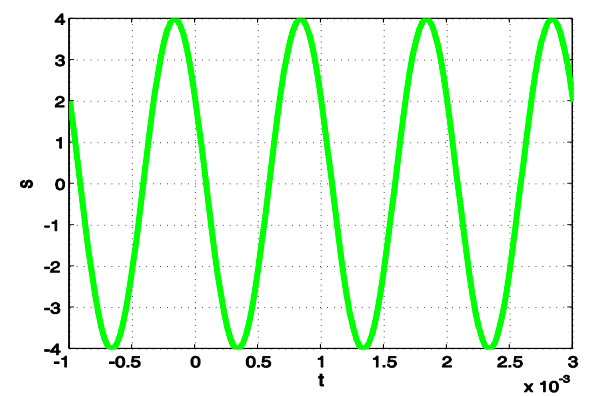
\includegraphics[width=0.5\textwidth]{harmonicky_signal_priebeh.png}
  \caption{Časový priebeh harmonického signálu $s(t) = 4\cos(2\pi \cdot 10^3 t + 0{,}3\pi)$}
\end{figure}

\textbf{Kvaziperiodický signál} je súčet harmonických signálov, pri ktorom aspoň dva kmitočty nemajú racionálny pomer -- inými slovami, nie je možné nájsť spoločný „základný" kmitočet, ktorého by boli všetky ostatné celistvými násobkami. Dôsledkom je, že signál sa nikdy presne nezopakuje, aj keď vizuálne vyzerá „takmer periodicky". Napriek tomu má, rovnako ako periodický signál, \textbf{čiarové (diskrétne) spektrum} -- energia je sústredená na konkrétnych diskrétnych kmitočtoch, nie rozložená spojito.

Príklad:
\begin{equation}
  s(t) = 2\cos(2\pi t) + 4\cos(t)
\end{equation}
kde pomer kmitočtov $2\pi / 1$ je iracionálne číslo.

\textbf{Neperiodický (aperiodický) signál} sa neopakuje vôbec -- buď existuje len v konečnom časovom úseku (impulz), alebo sa mení bez akejkoľvek pravidelnosti. Má \textbf{spojité spektrum} -- energia je rozložená plynulo po celej frekvenčnej osi.

\section{Výpočet výkonu}

Pre signál so zložitými hodnotami definujeme \textbf{normovaný okamžitý výkon} (pri $R=1\,\Omega$):
\begin{equation}
  p(t) = |s(t)|^2
\end{equation}

\textbf{Normovaná energia} signálu v intervale $\langle t_1, t_2 \rangle$:
\begin{equation}
  E = \int_{t_1}^{t_2} |s(t)|^2 \, dt
\end{equation}

\textbf{Stredný normovaný výkon} periodického signálu s periódou $T_1$:
\begin{equation}
  P_{\text{stř}} = \frac{1}{T_1} \int_0^{T_1} |s(t)|^2 \, dt
\end{equation}

Pre periodický signál vyjadrený Fourierovou radom $s(t) = \sum_{k=-\infty}^{\infty} c_k \exp(jk\omega_1 t)$ platí \textbf{Parsevalov teorém}:
\begin{equation}
  P_{\text{stř}} = \sum_{k=-\infty}^{\infty} |c_k|^2 = |c_0|^2 + 2\sum_{k=1}^{\infty} |c_k|^2
\end{equation}
Výkon teda možno vypočítať buď z časového priebehu (integrálom), alebo zo spektra (súčtom kvadrátov modulov koeficientov). Každý koeficient $|c_k|^2$ udáva, aká časť celkového výkonu pripadá na $k$-tú harmonickú zložku.

Pre aperiodický signál by bol stredný výkon nulový, pretože energia konečného impulzu sa pri delení nekonečne dlhým časovým intervalom blíži k nule. U aperiodických signálov preto hovoríme o \textbf{energii}, nie o výkone.

\section{Výpočet spektra}

\subsection{Fourierová rada -- periodické signály}

Každý periodický signál spĺňajúci Dirichletove podmienky možno rozložiť na súčet harmonických zložiek -- \textbf{Fourierova rada}:
\begin{equation}
  s(t) = \sum_{k=-\infty}^{+\infty} c_k \exp(jk\omega_1 t)
\end{equation}
Koeficienty $c_k$ (komplexné Fourierove koeficienty) sa vypočítajú:
\begin{equation}
  c_k = \frac{1}{T_1} \int_0^{T_1} s(t)\exp(-jk\omega_1 t)\,dt
\end{equation}
kde:
\begin{itemize}
  \item $k$ -- celé číslo, index harmonickej zložky,
  \item $\omega_1 = 2\pi/T_1$ -- základný uhlový kmitočet,
  \item $c_0$ -- jednosmerná (stredná) zložka signálu.
\end{itemize}
Množina koeficientov $\{c_k\}$ tvorí \textbf{frekvenčné spektrum} periodického signálu. Je to čiarové (diskrétne) spektrum -- kmitočtové zložky existujú len na celistvých násobkoch $\omega_1$.

\subsection{Fourierova transformácia -- aperiodické signály}

Pre aperiodické signály prechádzame k \textbf{Fourierovej transformácii} (FT):
\begin{equation}
  S(\omega) = \int_{-\infty}^{+\infty} s(t)\exp(-j\omega t)\,dt
\end{equation}
kde $S(\omega)$ je \textbf{spektrálna funkcia} (spojitá, komplexná). Inverzná FT:
\begin{equation}
  s(t) = \frac{1}{2\pi}\int_{-\infty}^{+\infty} S(\omega)\exp(j\omega t)\,d\omega
\end{equation}
Fyzikálna intuícia: keď zvyšujeme periódu periodického signálu $T_1 \to \infty$, čiary v spektre sa zhusťujú, až splynú do spojitého spektra.

\section{Typické príklady}

\subsection{Harmonický signál}

Harmonický signál $s(t) = C_1\cos(\omega_1 t + \varphi_1)$ má \textbf{čiarové spektrum} -- dve symetrické čiary na kmitočtoch $\pm\omega_1$ s amplitúdami $C_1/2$.

\begin{figure}[H]
  \centering
  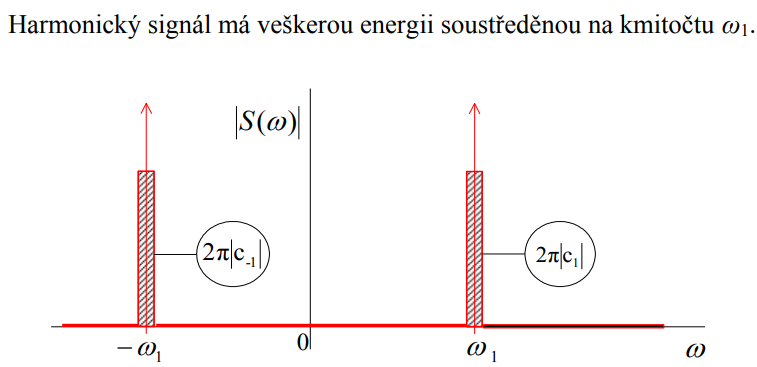
\includegraphics[width=0.82\textwidth]{harmonicky_signal_spektrum.png}
  \caption{Amplitúdové (čiarové) frekvenčné spektrum harmonického signálu -- dve symetrické čiary na $\pm\omega_1$}
\end{figure}

\subsection{Periodický sled obdĺžnikových impulzov}

Pre periodický sled obdĺžnikov (perióda $T_1$, šírka $\vartheta$, výška $D$) platí:
\begin{equation}
  c_k = D\frac{\vartheta}{T_1}\,\text{sinc}\!\left(\frac{\vartheta}{2}\,k\omega_1\right), \qquad
  \text{kde } \text{sinc}(x) = \frac{\sin x}{x}
\end{equation}
kde:
\begin{itemize}
  \item $c_k$ -- $k$-ty Fourierov koeficient,
  \item $D\vartheta/T_1$ -- jednosmerná hodnota (stredná hodnota signálu),
  \item $\vartheta/2 \cdot k\omega_1$ -- argument funkcie sinc, ktorý určuje kde sú nuly obálky.
\end{itemize}
Spektrum je čiarové, obálka čiar má tvar funkcie sinc. Prvá nula obálky je na $\omega_a = 2\pi/\vartheta$. Čím užší je impulz (menšie $\vartheta$), tým širšie je spektrum.

\begin{figure}[H]
  \centering
  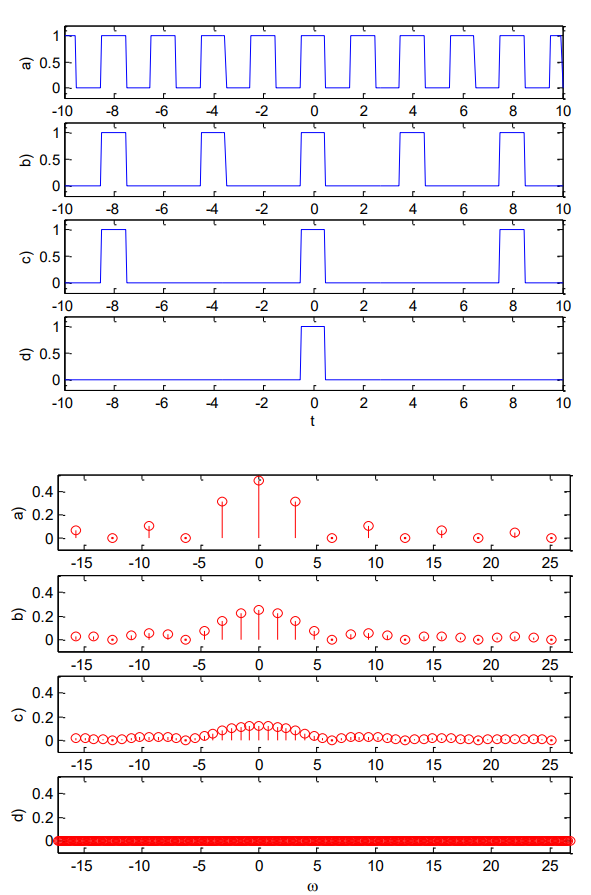
\includegraphics[width=0.82\textwidth]{periodicky_sled_obdlznikov_a_spektra.png}
  \caption{Periodický sled obdĺžnikových impulzov s parametrami $T_1$, $\vartheta$, $D$ a výpočet koeficientov Fourierovej rady}
\end{figure}

\subsection{Obdĺžnikový impulz}

Obdĺžnikový impulz so šírkou $\vartheta$ a výškou $D$, symetrický okolo $t=0$, má spektrum:
\begin{equation}
  S(\omega) = D\vartheta\,\text{sinc}\!\left(\frac{\vartheta}{2}\,\omega\right)
\end{equation}
kde:
\begin{itemize}
  \item $D\vartheta$ -- plocha impulzu (hodnota spektra pri $\omega=0$),
  \item $\vartheta/2\,\omega$ -- argument funkcie sinc.
\end{itemize}
Širší impulz $\Rightarrow$ užšie spektrum, užší impulz $\Rightarrow$ širšie spektrum. Asi 90\,\% energie leží v pásme $|\omega| < 2\pi/\vartheta$.

\begin{figure}[H]
  \centering
  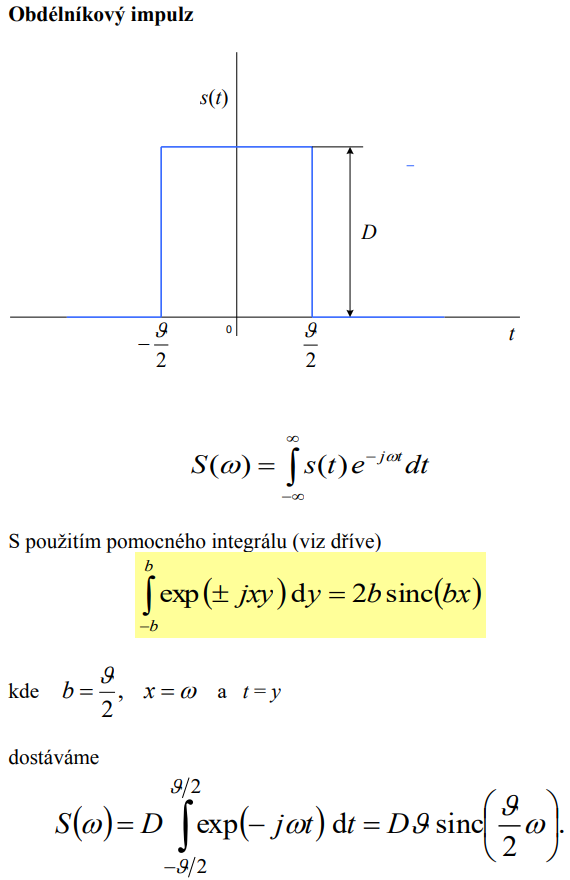
\includegraphics[width=0.7\textwidth]{obdlznikovy_impulz_spektrum_sinc.png}
  \caption{Obdĺžnikový impulz (vľavo) a jeho spojité amplitúdové spektrum tvaru sinc (vpravo)}
\end{figure}

\subsection{Harmonický impulz}

Harmonický impulz (rádiový impulz) je harmonický signál s krátkym trváním:
\begin{equation}
  s(t) = \begin{cases} A\cos(\omega_0 t) & \text{pre } |t| \leq \tau/2 \\ 0 & \text{inak} \end{cases}
\end{equation}
kde $A$ je amplitúda, $\omega_0$ je nosný kmitočet a $\tau$ je trvanie impulzu. Spektrum je sústredené okolo $\pm\omega_0$, s tvarom sinc. Čím dlhší impulz, tým užšie spektrum a tým viac sa blíži čiarovému spektru harmonického signálu.

\begin{figure}[H]
  \centering
  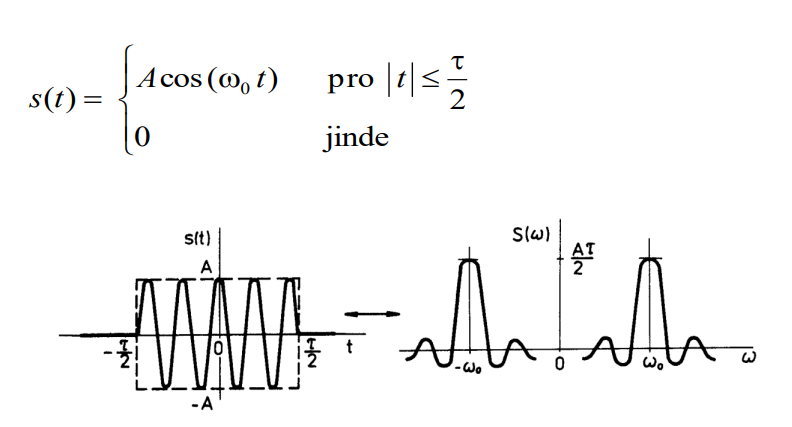
\includegraphics[width=0.82\textwidth]{harmonicky_impulz_spektrum.png}
  \caption{Harmonický (rádiový) impulz -- časový priebeh (vľavo) a jeho amplitúdové spektrum sústredené okolo $\pm\omega_0$ (vpravo)}
\end{figure}

% ============================================================
\chapter{Prevody medzi analógovými a digitálnymi signálmi; vzorkovanie, aliasing; rovnomerné a nerovnomerné kvantovanie; kvantovací šum}
% ============================================================

\section{Reťazec A/D prevodu}

Analogovo-číslicový (A/D) prevod prebieha v troch krokoch:
\begin{equation}
  s(t) \;\xrightarrow{\text{vzorkovanie}}\; \xrightarrow{\text{kvantovanie}}\; \xrightarrow{\text{kódovanie}}\; s(n)
\end{equation}

\section{Vzorkovanie}

\textbf{Ideálne vzorkovanie} spočíva v násobení spojitého signálu $s(t)$ radom Diracových impulzov so vzájomným odstupom $T$:
\begin{equation}
  s_v(t) = s(t) \cdot \sum_{n=-\infty}^{+\infty} \delta(t - nT)
         = \sum_{n=-\infty}^{+\infty} s(nT)\,\delta(t - nT)
\end{equation}

\begin{figure}[H]
  \centering
  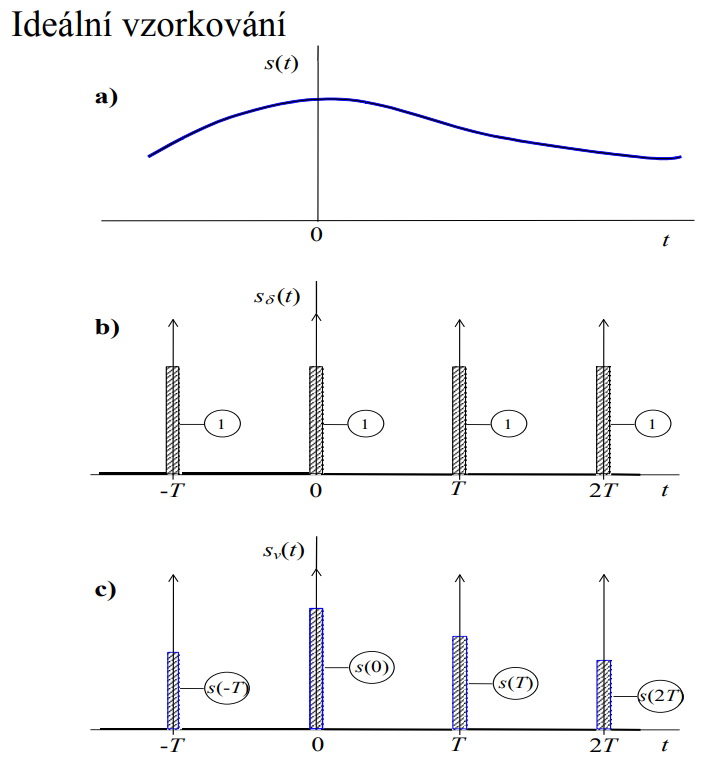
\includegraphics[width=0.7\textwidth]{idealne_vzorkovanie_casova_oblast.png}
  \caption{Ideálne vzorkovanie v časovej oblasti: a) pôvodný spojitý signál $s(t)$, b) sled jednotkových impulzov $s_\delta(t)$, c) vzorkovaný signál $s_v(t)$}
\end{figure}

Dôsledok v kmitočtovej oblasti: \textbf{periodizácia spektra} pôvodného signálu s periódou $\omega_1 = 2\pi/T$:
\begin{equation}
  S_v(\omega) = \frac{1}{T}\sum_{k=-\infty}^{+\infty} S(\omega - k\omega_1)
\end{equation}
Spektrum navzorkovaného signálu je teda nekonečná suma posunutých kópií pôvodného spektra, výškovo znížená faktorom $1/T$.

\section{Vzorkovací teorém}

\textbf{Vzorkovací teorém} (Nyquistov / Shannonov / Kotelníkův): Signál $s(t)$ so spektrom obmedzeným horným medzným kmitočtom $f_m$ možno jednoznačne vyjadriť postupnosťou vzoriek $\{s(nT)\}$, ak je splnená podmienka:
\begin{equation}
  \boxed{f_{\text{vz}} > 2f_m}
\end{equation}
kde $f_{\text{vz}} = 1/T$ je vzorkovací kmitočet a $f_m$ je horný medzný kmitočet spektra analógového signálu. Kmitočet $2f_m$ sa nazýva \textbf{Nyquistov kmitočet}.

\begin{figure}[H]
  \centering
  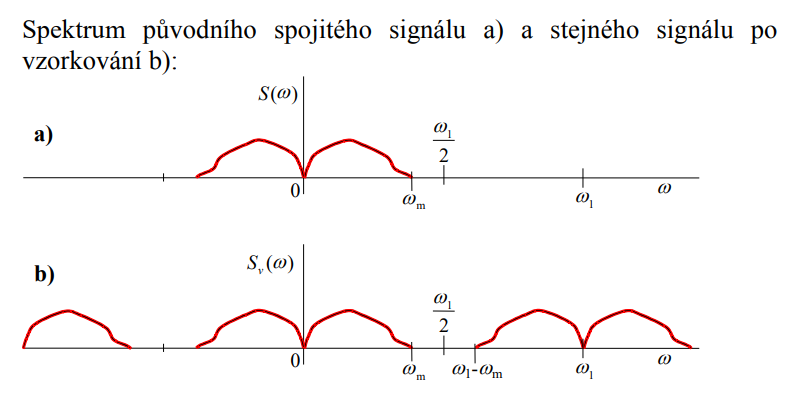
\includegraphics[width=0.82\textwidth]{spektrum_pred_a_po_vzorkovani_korektne.png}
  \caption{Spektrum pôvodného spojitého signálu $S(\omega)$ (hore) a spektrum navzorkovaného signálu $S_v(\omega)$ (dole) pri splnení vzorkovacieho teorému -- spektrá sa neprekrývajú}
\end{figure}

\section{Aliasing}

Ak podmienka vzorkovacieho teorému nie je splnená ($f_{\text{vz}} < 2f_m$), periodické kópie spektra sa začnú \textbf{prekrývať}. Tento jav sa nazýva \textbf{aliasing}. V kmitočtovej oblasti dochádza k sčítaniu zložiek z rôznych kópií spektra, čo spôsobuje nenahraditeľnú stratu informácie. V časovej oblasti sa aliasing prejaví zmenou tvaru rekonštruovaného signálu -- rôzne signály s rôznym kmitočtom produkujú rovnaké vzorky.

\begin{figure}[H]
  \centering
  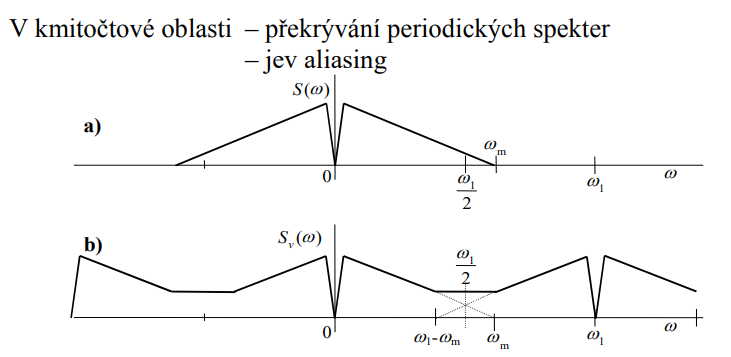
\includegraphics[width=0.82\textwidth]{aliasing_prekrytie_spektier.png}
  \caption{Aliasing -- prekrytie spektier pri nesplnení vzorkovacieho teorému: a) pôvodné spektrum $S(\omega)$, b) spektrum $S_v(\omega)$ s prekrytím (aliasing)}
\end{figure}

Obrana proti aliasingu: zvýšiť vzorkovací kmitočet $f_{\text{vz}}$, alebo pred vzorkovaním zaradiť \textbf{antialiasingový filter} (AAF, dolná priepusť s medzným kmitočtom $f_m < f_{\text{vz}}/2$), ktorý odreže frekvenčné zložky, ktoré by spôsobili aliasing.

\begin{figure}[H]
  \centering
  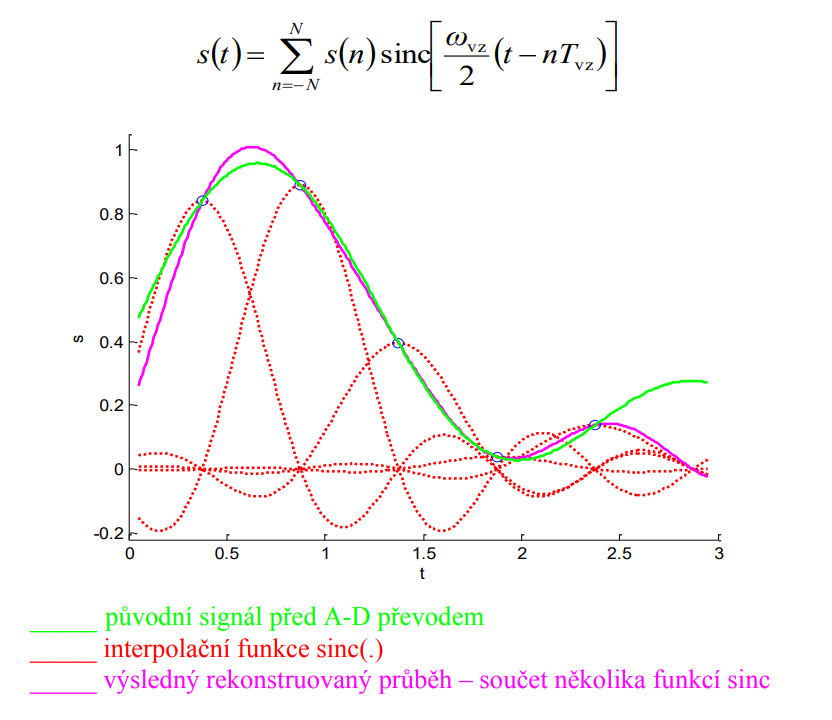
\includegraphics[width=0.82\textwidth]{rekonstrukcia_signal_zo_vzoriek.png}
  \caption{Vplyv antialiasingového filtra (AAF): a) spektrum signálu pred filtrovaním, b) spektrum navzorkovaného signálu po AAF -- spektrá sa neprekrývajú a rekonštrukcia je možná}
\end{figure}

\textbf{Rekonštrukcia signálu zo vzoriek:} Po správnom vzorkovaní možno pôvodný spojitý signál zrekonštruovať pomocou ideálnej dolnej priepuste s medzným kmitočtom $f_{\text{vz}}/2$. V praxi sa používajú rekonstrukčné (vyhladzovacia) filtre zaradené za D/A prevodník. Čím vyšší je vzorkovací kmitočet nad Nyquistovu hranicu, tým jednoduchší (menej strmý) rekonštrukčný filter postačuje.

\section{Kvantovanie}

\textbf{Kvantovanie} je zaokrúhlenie spojitých hodnôt vzoriek na konečný počet diskrétnych úrovní. Počet kvantovacích úrovní:
\begin{equation}
  N = 2^b
\end{equation}
kde $b$ je počet bitov na vzorku. Kvantovací krok (rozlíšenie):
\begin{equation}
  \Delta s = \frac{\text{Rozsah}}{2^b} = \frac{U_{\max} - U_{\min}}{2^b}
\end{equation}
kde:
\begin{itemize}
  \item $\Delta s$ -- veľkosť jedného kvantovacieho kroku,
  \item $U_{\max}, U_{\min}$ -- krajné hodnoty vstupného signálu,
  \item $b$ -- počet bitov (každý bit zdvojnásobí počet úrovní a zmenší $\Delta s$ na polovicu).
\end{itemize}

\begin{figure}[H]
  \centering
  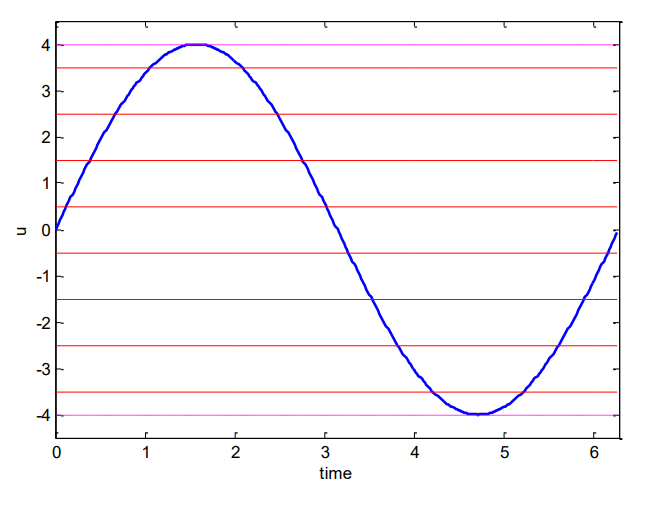
\includegraphics[width=0.7\textwidth]{kvantizacny_krok_pocet_bitov.png}
  \caption{Kvantovanie harmonického signálu -- sínusový priebeh s vyznačenými kvantovacími hladinami, $N = 2^b$ úrovní, kvantovací krok $\Delta s = \text{Rozsah}/2^b$}
\end{figure}

\section{Kvantovací šum}

Rozdiel medzi pôvodným signálom a kvantovaným signálom je \textbf{kvantovací šum}:
\begin{equation}
  r(t) = s(t) - s_{kv}(t)
\end{equation}
Šum $r(t)$ má pilovitý priebeh s amplitúdou $\pm\Delta s/2$.

\begin{figure}[H]
  \centering
  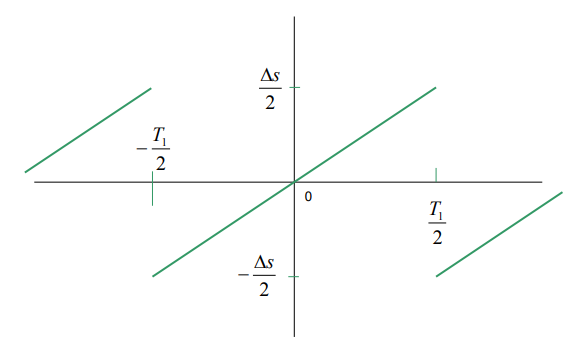
\includegraphics[width=0.82\textwidth]{kvantizacny_sum_priebeh.png}
  \caption{Kvantovací šum -- časový priebeh pôvodného signálu $s(t)$ a kvantovaného signálu $s_{kv}(t)$ (hore) a výsledný šum $r(t) = s(t) - s_{kv}(t)$ (dole)}
\end{figure}

Efektívna hodnota kvantovacieho šumu (odvodená pre pilovitý priebeh):
\begin{equation}
  R_{\text{ef}}^2 = \frac{1}{T_1}\int_{-T_1/2}^{T_1/2}\!\!\left(\frac{\Delta s}{T_1}t\right)^2\!dt
  = \frac{(\Delta s)^2}{12}
  \qquad\Rightarrow\qquad
  R_{\text{ef}} = \frac{\Delta s}{\sqrt{12}}
\end{equation}

\begin{figure}[H]
  \centering
  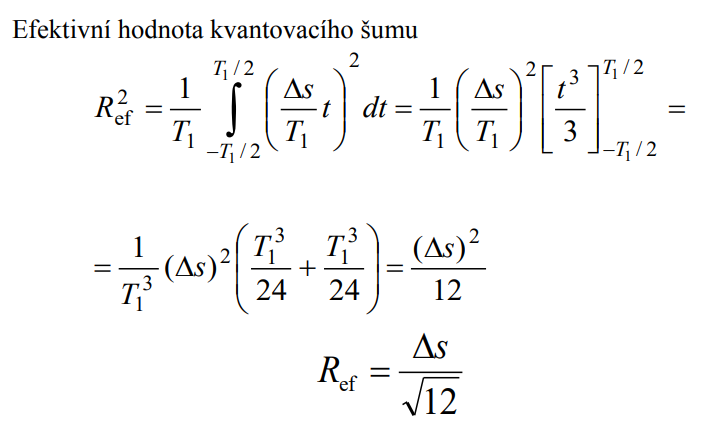
\includegraphics[width=0.7\textwidth]{kvantizacny_sum_odvodenie.png}
  \caption{Náhrada kvantovacieho šumu pilovitým priebehom -- základ pre výpočet efektívnej hodnoty $R_{\text{ef}} = \Delta s / \sqrt{12}$ a činiateľa zkreslenia}
\end{figure}

\textbf{Pomer signál/šum (SNR)} pre harmonický vstupný signál s amplitúdou $S_{\max}$ ($S_{\text{ef}} = S_{\max}/\sqrt{2}$):
\begin{align}
  \text{SNR} &= \frac{S_{\text{ef}}^2}{R_{\text{ef}}^2}
    = \frac{S_{\max}^2/2}{(\Delta s)^2/12}
    = \frac{6\,S_{\max}^2}{(\Delta s)^2}
\end{align}
Po dosadení $\Delta s = 2S_{\max}/2^b$ a vyjadrení v decibeloch dostaneme praktický vzorec:
\begin{equation}
  \boxed{\text{SNR} = 6{,}021\cdot b + 1{,}761 \quad [\text{dB}]}
\end{equation}
kde $b$ je počet bitov. Každý pridaný bit zvýši SNR o približne 6\,dB.

\section{Nerovnomerné kvantovanie}

Pri \textbf{rovnomernom kvantovaní} je $\Delta s$ konštantný pre všetky úrovne. Pre slabé signály je relatívna chyba kvantizácie väčšia ako pre silné signály -- to je nevýhoda napr. pri prenose reči, kde dominujú tiché pasáže.

\textbf{Nerovnomerné kvantovanie} rieši tento problém: jemnejšie kroky pre malé hodnoty, hrubšie kroky pre veľké hodnoty. Prakticky sa realizuje kombináciou \textbf{kompresora} a rovnomerného kvantizéra -- spolu tvoria \textbf{kompandér}.

\begin{figure}[H]
  \centering
  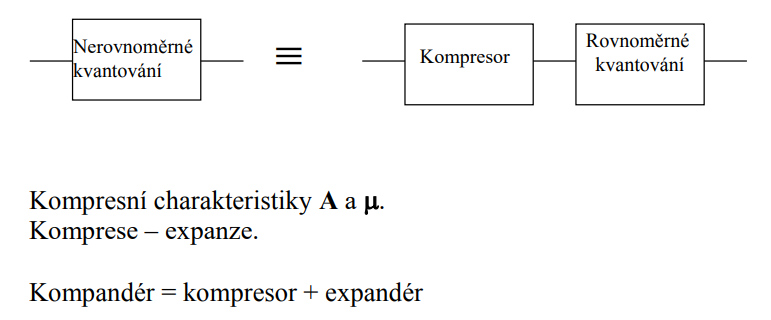
\includegraphics[width=0.82\textwidth]{nerovnomerne_kvantovanie_schema.png}
  \caption{Nerovnomerné kvantovanie -- schéma ekvivalencie: nerovnomerný kvantizér $\equiv$ kompresor + rovnomerný kvantizér}
\end{figure}

\section{Kódovanie}

\textbf{Kódovanie} je posledný krok A/D prevodu -- každej kvantovanej vzorke sa priradí binárne číslo (postupnosť núl a jedničiek). Najjednoduchší je \textbf{priamy dvojkový kód} (Natural Binary Code), kde každej úrovni zodpovedá jej binárna reprezentácia. Napríklad pre $b=3$ bity a $N=8$ úrovní: úroveň 0 = \texttt{000}, úroveň 5 = \texttt{101}, atď. Spôsob kódovania možno voliť podľa rôznych kritérií -- najčastejšie podľa dĺžky série alebo odolnosti proti rušeniu pri prenose (napr. Grayov kód, BCD).

\begin{figure}[H]
  \centering
  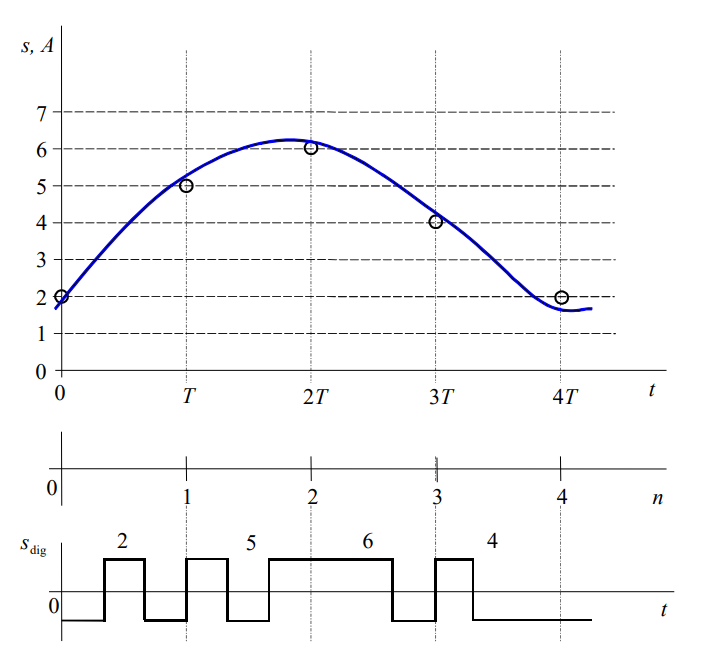
\includegraphics[width=0.82\textwidth]{AD_prevod_kodovanie.png}
  \caption{Kódovanie pri A/D prevode -- sínusový signál so vzorkami, číslicová postupnosť hodnôt vzoriek a priamy dvojkový kód pre $b = 3$ bity ($N = 8$ úrovní)}
\end{figure}

% ============================================================
\chapter{Lineárne a nelineárne systémy; vplyv nelinearity na spektrum; stabilné, kauzálne a časovo invariantné systémy; testovací signály}
% ============================================================

\section{Lineárne a nelineárne systémy}

Sústava je \textbf{lineárna}, ak platí \textbf{princíp superpozície} -- teda ak sústava reaguje na súčet viacerých vstupných signálov rovnako, ako keby sme sčítali jej odpovede na každý vstup zvlášť:
\begin{equation}
  ax_1(t) + bx_2(t) \;\rightarrow\; ay_1(t) + by_2(t)
\end{equation}
kde $a, b$ sú reálne konštanty, $x_1, x_2$ sú vstupné signály a $y_1, y_2$ sú zodpovedajúce výstupné signály. Princíp superpozície zahŕňa aj násobenie vstupného signálu konštantou (homogenita) aj sčítanie vstupov (aditivita).

\textbf{Nelineárna sústava} princíp superpozície nespĺňa.

\section{Vplyv linearity/nelinearity na spektrum}

\begin{itemize}
  \item \textbf{Lineárna sústava:} spektrum sa nezmení -- môžu byť potlačené alebo zosilnené niektoré existujúce zložky, ale \emph{nové kmitočtové zložky nevznikajú}.
  \item \textbf{Nelineárna sústava:} spektrum sa \emph{obohatí o nové zložky} -- harmonické skreslenie, intermodulácia. Na výstupe sa objavia zložky, ktoré na vstupe neboli.
\end{itemize}

\textbf{Príklad -- nelineárna sústava s kvadratickou charakteristikou:}

Na vstup sústavy $y(x) = a_1 x + a_2 x^2$ privedieme harmonický signál $x(t) = C\cos\omega_1 t$. Výstup:
\begin{align}
  y(t) &= a_1 C\cos\omega_1 t + a_2 C^2\cos^2\omega_1 t \notag \\
       &= \underbrace{\frac{1}{2}a_2 C^2}_{\text{jednosm.}}
         + \underbrace{a_1 C\cos\omega_1 t}_{\text{zložka }\omega_1}
         + \underbrace{\frac{1}{2}a_2 C^2\cos 2\omega_1 t}_{\text{nová zložka }2\omega_1}
\end{align}
Na vstupe bola jedna čiara ($\omega_1$), na výstupe sú tri: jednosmerná zložka, $\omega_1$ a nová $2\omega_1$.

\begin{figure}[H]
  \centering
  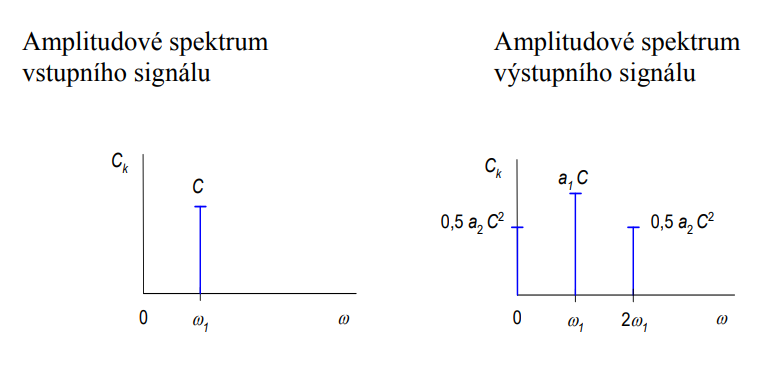
\includegraphics[width=0.82\textwidth]{nelinearny_system_amplitudove_spektrum.png}
  \caption{Amplitúdové spektrum na vstupe (jedna čiara na $\omega_1$) a na výstupe nelineárnej sústavy (jednosmerná zložka + $\omega_1$ + nová $2\omega_1$)}
\end{figure}

\section{Základné vlastnosti LSI sústav}

Sústava je \textbf{LSI} (lineárna, stabilná, časovo invariantná), ak spĺňa:

\begin{enumerate}
  \item \textbf{Linearita} -- platí princíp superpozície (viď vyššie).

  \item \textbf{Časová invariancia} -- posunutie vstupného signálu v čase o $\tau$ spôsobí rovnaké posunutie výstupného signálu:
  \begin{equation}
    x(t-\tau) \;\rightarrow\; y(t-\tau)
  \end{equation}
  Sústava sa teda nemení v čase -- jej parametre sú konštantné.

  \item \textbf{Stabilita} -- pre každý ohraničený vstup je výstup tiež ohraničený (podmienka BIBO -- Bounded Input, Bounded Output):
  \begin{equation}
    |x(t)|_{\max} \leq A < \infty \;\Rightarrow\; |y(t)|_{\max} \leq B < \infty
  \end{equation}

  \item \textbf{Kauzalita} -- výstup v čase $t_0$ nezávisí na budúcich hodnotách vstupu ($t > t_0$). Každá fyzikálne realizovateľná sústava je kauzálna.
\end{enumerate}

\section{Impulzná charakteristika a konvolúcia}

\textbf{Impulzná charakteristika} $h(t)$ je odozva LSI sústavy na \textbf{jednotkový impulz} $\delta(t)$ privedený na vstup:
\begin{equation}
  \delta(t) \;\rightarrow\; [\text{LSI}] \;\rightarrow\; h(t)
\end{equation}

Keďže každý signál možno rozložiť na sled impulzov rôznej váhy, stačí vedieť, ako sústava reaguje na jeden impulz -- teda poznať $h(t)$. Výstup pre ľubovoľný vstup $x(t)$ je potom \textbf{konvolúcia} vstupu s impulznou charakteristikou:
\begin{equation}
  y(t) = h(t) * x(t) = \int_0^{t} h(\tau)\,x(t-\tau)\,d\tau
\end{equation}

\section{Prechodová charakteristika}

\textbf{Prechodová charakteristika} $g(t)$ je odozva LSI sústavy na \textbf{jednotkový skok} $\sigma(t)$:
\begin{equation}
  \sigma(t) \;\rightarrow\; [\text{LSI}] \;\rightarrow\; g(t)
\end{equation}

Impulzná a prechodová charakteristika sú navzájom prepojené -- keďže jednotkový skok je integrálom jednotkového impulzu, platí:
\begin{equation}
  h(t) = g'(t) \qquad \Leftrightarrow \qquad g(t) = \int_0^t h(\tau)\,d\tau
\end{equation}

\section{Testovací signály}

Na testovanie a analýzu LSI sústav sa používajú štandardné \textbf{testovacie signály}:

\begin{itemize}
  \item \textbf{Jednotkový impulz} $\delta(t)$: Diracov impulz, konečná plocha v nulovom čase. Odozva naň je impulzná charakteristika $h(t)$ -- teda kompletný popis sústavy.

  \item \textbf{Jednotkový skok} $\sigma(t)$: signál skočí z 0 na 1 v čase $t=0$. Odozva naň je prechodová charakteristika $g(t)$. Definícia a varianty jednotkového skoku:

\begin{figure}[H]
  \centering
  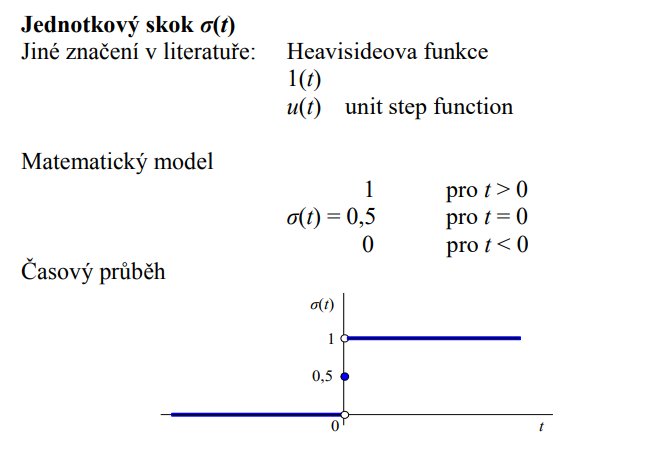
\includegraphics[width=0.82\textwidth]{jednotkovy_skok_priebeh.png}
  \caption{Jednotkový skok $\sigma(t)$ -- základný časový priebeh (hodnota 0 pre $t<0$, hodnota 1 pre $t>0$)}
\end{figure}

\begin{figure}[H]
  \centering
  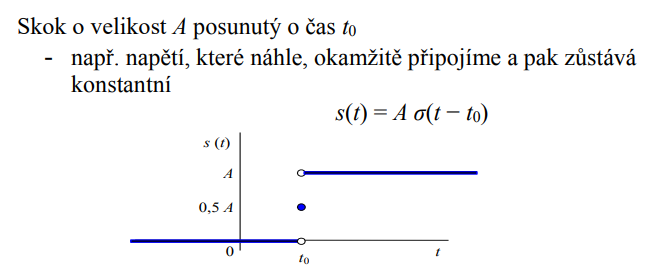
\includegraphics[width=0.82\textwidth]{posunuty_jednotkovy_skok_priebeh.png}
  \caption{Posunutý jednotkový skok $s(t) = A\,\sigma(t - t_0)$ -- skok o veľkosť $A$ posunutý o čas $t_0$}
\end{figure}

\begin{figure}[H]
  \centering
  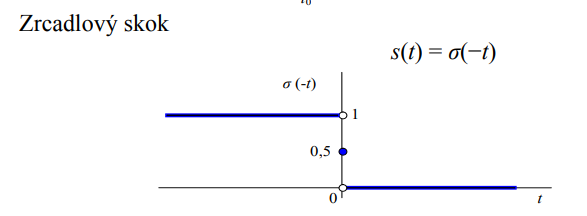
\includegraphics[width=0.82\textwidth]{zrkadlovy_skok_priebeh.png}
  \caption{Zrkadlový (časovo obrátený) skok $s(t) = \sigma(-t)$ -- zrkadlový obraz jednotkového skoku}
\end{figure}

  \item \textbf{Harmonický signál} $x(t) = C\cos(\omega_1 t + \varphi_1)$: najdôležitejší testovací signál v praxi. Odozva LSI sústavy na harmonický signál je \emph{opäť harmonický signál rovnakého kmitočtu}, ale so zmenenou amplitúdou a fázou. Závislosť amplitúdy a fázy od kmitočtu opisuje \textbf{frekvenčná charakteristika} $H(j\omega)$.

\begin{figure}[H]
  \centering
  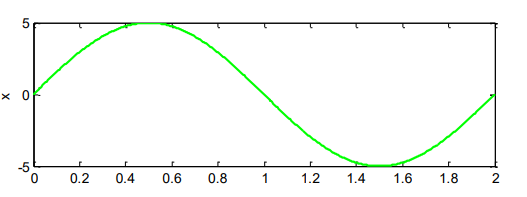
\includegraphics[width=0.82\textwidth]{harmonicky_testovaci_signal.png}
  \caption{Harmonický ustálený stav v LSI sústave -- vstupný harmonický signál $x(t)$ a výstupný signál $y(t)$ rovnakého kmitočtu so zmenenou amplitúdou a fázou}
\end{figure}

\end{itemize}


	%\documentclass[12pt,a4paper]{report}
%
%% --- Kódovanie a jazyk ---
%\usepackage[utf8]{inputenc}
%\usepackage[T1]{fontenc}
%\usepackage[english]{babel}
%
%% --- Matematika ---
%\usepackage{amsmath}
%\usepackage{amssymb}
%
%% --- Obrázky ---
%\usepackage{graphicx}
%\usepackage{float}
% !TeX spellcheck = sk_SK-Slovak
% !TeX root = statnicaEKT.tex
\graphicspath{{./Obrazky/SI2/}}

% --- Placeholder príkaz ---
\newcommand{\imgplaceholder}[1]{%
  \begin{figure}[H]
    \centering
    \fbox{\parbox{0.7\textwidth}{\centering\vspace{1cm}
    \texttt{[OBRÁZOK: #1]}\vspace{1cm}}}
    \caption{#1}
  \end{figure}
}

% --- Ďalšie balíčky ---
%\usepackage{booktabs}   % krajšie tabuľky
%\usepackage{array}
%\usepackage{geometry}
%\geometry{margin=2.5cm}
%\usepackage{hyperref}
%\usepackage{parskip}
%\setlength{\parskip}{6pt}
%
%% ============================================================
%\begin{document}
% ============================================================

% --- Titulná strana ---
%\begin{titlepage}
%  \centering
%  \vspace*{3cm}
%  {\LARGE\bfseries BPC-SI2 -- Signály 2\\[0.5em]}
%  {\large Vypracovanie okruhov na skúšku}
%  \vfill
%  {\large \today}
%\end{titlepage}

% ============================================================
\part{BPC-SI2 -- Signály 2}

\begin{huge}
  Otázky:
  \newline
\end{huge}

\begin{enumerate}
  \item Otázka -- Náhodné signály: definícia, parametre a charakteristiky,
        stacionárny a ergodický signál, spektrum.
  \item Otázka -- Lineárna filtrácia signálov: filtre FIR a IIR,
        vlastnosti, metódy návrhu, spôsoby realizácie.
  \item Otázka -- Lineárna predikcia signálu: definícia, využitie pre
        reštauráciu signálu a získanie spektra, význam pre rozpoznávanie reči.
\end{enumerate}

\newpage

% ============================================================
% OKRUH 1
% ============================================================
\chapter{Náhodné signály}

% ------------------------------------------------------------
\section{Čo je náhodný signál}
% ------------------------------------------------------------

Deterministický signál vieme v každom okamihu presne vypočítať --- poznáme
jeho matematický popis s pevnými parametrami. Náhodný (stochastický) signál
takúto vlastnosť nemá: jeho okamžitá hodnota je nepredvídateľná, nesie určitú
mieru neurčitosti. Napriek tomu ho možno charakterizovať štatistickými
vlastnosťami, ktoré zostávajú dlhodobo stálé. Prakticky: väčšina reálnych
signálov obsahuje prvky náhodnosti (šum, rušenie, neznáma informácia), lebo
v prírode neexistujú fyzikálne deje bez prvkov náhody. Spracovanie náhodných
signálov sa opiera o teóriu pravdepodobnosti a matematickú štatistiku.

\begin{figure}[H]
  \centering
  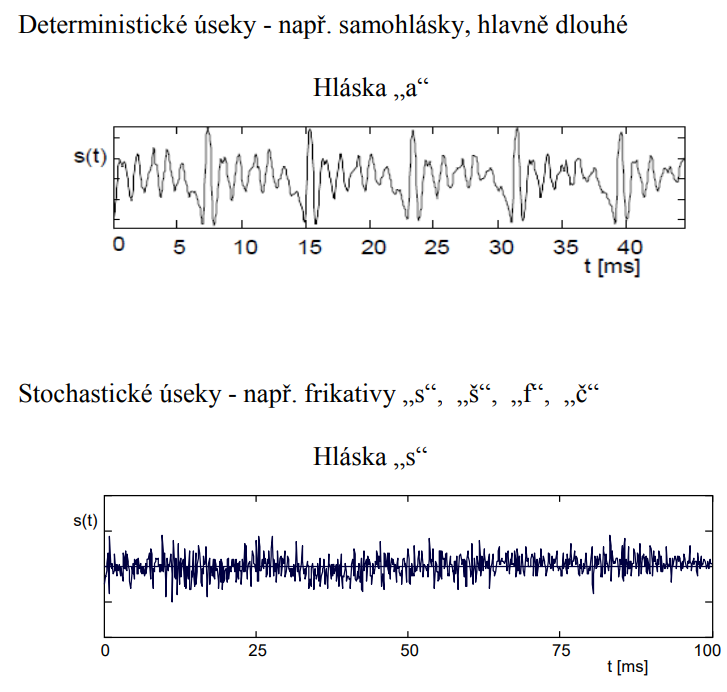
\includegraphics[width=0.82\textwidth]{hlaska_a_hlaska-s.png}
  \caption{Priebeh rečového signálu -- hláska ,,a'' (periodický, znelý úsek) a hláska ,,s'' (šumový, neznelý úsek).}
\end{figure}

% ------------------------------------------------------------
\section{Náhodná veličina a jej popis}
% ------------------------------------------------------------

Náhodný jav je idealizovaný výsledok pokusu (napr. hod kockou, nameraná hodnota
šumu). Keď výsledku pokusu priradíme číslo, hovoríme o \textbf{náhodnej
veličine} --- tá môže byť diskrétna (napr. číslo na kocke) alebo spojitá
(napr. okamžité napätie šumu).

\subsection{Hustota rozdelenia pravdepodobnosti}

Hustota rozdelenia pravdepodobnosti $p(x)$ pre spojitú náhodnú veličinu $\xi$
--- predstav si ju ako krivku, ktorá hovorí, kde sa hodnoty veličiny ,,radi
zdržiavajú''. Vysoká hodnota $p(x)$ na nejakom $x$ znamená, že táto hodnota
nastáva často; nízka znamená, že je zriedkavá. Platia pre ňu tri základné
vlastnosti:
\begin{itemize}
  \item $p(x) \geq 0$ \quad (pravdepodobnosť nemôže byť záporná)
  \item Pravdepodobnosť, že $\xi$ padne do intervalu $\langle a,b\rangle$:
    \[
      P(a \leq \xi \leq b) = \int_a^b p(x)\, dx
    \]
  \item Pravdepodobnosť, že $\xi$ je kdekoľvek, musí byť 1:
    \[
      P(-\infty < \xi < \infty) = \int_{-\infty}^{+\infty} p(x)\, dx = 1
    \]
\end{itemize}

\subsection{Distribučná funkcia}

Distribučná funkcia $F(x) = P(\xi < x)$ je kumulatívna suma hustoty ---
hovorí, aká je pravdepodobnosť, že veličina nadobudne hodnotu menšiu ako $x$.
Je to neklesajúca funkcia, $F(-\infty) = 0$, $F(+\infty) = 1$. Platí:
\[
  p(x) = \frac{dF(x)}{dx}, \qquad F(x) = \int_{-\infty}^{x} p(\alpha)\, d\alpha
\]
Pre diskrétnu veličinu má tvar schodovej funkcie, pre spojitú plynulej krivky.

\begin{figure}[H]
  \centering
  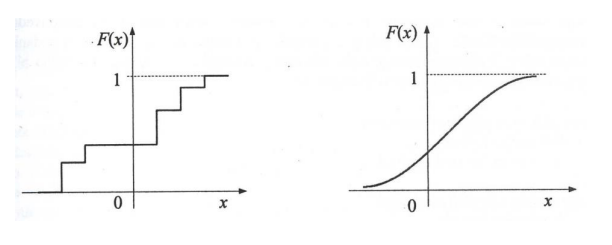
\includegraphics[width=0.82\textwidth]{diskretna_a_spojita_distribucna_funkcia.png}
  \caption{Distribučná funkcia $F(x)$ pre diskrétnu (schodovitá) a spojitú (plynulá) náhodnú veličinu.}
\end{figure}

\subsection{Normálne (Gaussovo) rozdelenie}

Najdôležitejší typ rozdelenia v praxi:
\[
  p(x) = \frac{1}{\sigma\sqrt{2\pi}}
  \exp\!\left[-\frac{(x-\mu)^2}{2\sigma^2}\right]
\]
kde:
\begin{itemize}
  \item $\mu$ --- stredná hodnota [rovnaká jednotka ako $x$]: poloha vrcholu
        krivky (kde sa hodnoty najviac sústreďujú)
  \item $\sigma$ --- smerodajná odchýlka [rovnaká jednotka ako $x$]: šírka
        krivky (čím väčšia $\sigma$, tým ,,rozliata'' krivka, tým väčší
        rozptyl hodnôt)
\end{itemize}
Gaussovo rozdelenie je kľúčové, pretože mnohé reálne šumy ho spĺňajú (napr.
tepelný šum rezistoru). Pre $\mu = 0$ a $\sigma = 1$ ide o normované normálne
rozdelenie.

% ------------------------------------------------------------
\section{Momenty -- číselné charakteristiky náhodnej veličiny}
% ------------------------------------------------------------

Namiesto úplného popisu pomocou $p(x)$ stačí v praxi poznať niekoľko
číselných charakteristík nazývaných \textbf{momenty}. Čím vyšší rád momentu,
tým ,,jemnejšiu'' vlastnosť rozdelenia popisuje.

\subsection{Obecný moment $k$-tého rádu}

Hovorí, aká je priemerná hodnota $x^k$, váhovaná hustotou. Pre spojitú
veličinu:
\[
  m_k = \int_{-\infty}^{+\infty} x^k \, p(x)\, dx
\]
Pre diskrétnu veličinu s možnými hodnotami $x_i$ a pravdepodobnosťami
$P\{x_i\}$:
\[
  m_k = \sum_{i} x_i^k \, P\{x_i\}
\]
kde $x_i$ sú jednotlivé možné hodnoty veličiny a $P\{x_i\}$ je pravdepodobnosť
výskytu hodnoty $x_i$.

\subsection{Centrálny moment $k$-tého rádu}

To isté, ale odčítame strednú hodnotu $\mu$ --- meriame odchýlky od stredu.
Pre spojitú veličinu:
\[
  m_k = \int_{-\infty}^{+\infty} (x - \mu)^k \, p(x)\, dx
\]
Pre diskrétnu veličinu:
\[
  m_k = \sum_{i} (x_i - \mu)^k \, P\{x_i\}
\]

Zmysel: obecný moment $m_1$ nám dá strednú hodnotu, ale ak chceme vedieť, ako
sú hodnoty \emph{rozptýlené okolo stredu}, potrebujeme centrálne momenty (kde
od každej hodnoty $x_i$ najprv odčítame stred $\mu$).

\subsection{Najdôležitejšie momenty}

\begin{itemize}
  \item $m_1$ (obecný, $k=1$) $= \mu$ \textbf{-- stredná hodnota}: priemerná
        hodnota, ťažisko rozdelenia
  \item $m_2$ (centrálny, $k=2$) $= D$ \textbf{-- disperzia (rozptyl)}: priemerná
        kvadratická odchýlka od $\mu$ --- miera toho, ako sú hodnoty
        ,,roztrúsené'' okolo stredu; jednotka je $[x]^2$
  \item $m_3$ (centrálny, $k=3$) -- \textbf{šikmosť}: miera nesymetrie
        rozdelenia okolo stredu
  \item $m_4$ (centrálny, $k=4$) -- \textbf{špičatosť}: miera toho, či je
        rozdelenie zaostrejšie alebo plochejšie ako Gaussovo
\end{itemize}

\textbf{Smerodajná odchýlka}: $\sigma = \sqrt{D}$ --- má rovnaké jednotky
ako signál, priamo interpretovateľná ako ,,typická odchýlka'' od strednej
hodnoty.

% ------------------------------------------------------------
\section{Náhodný proces}
% ------------------------------------------------------------

Náhodný signál popisujeme pojmom \textbf{náhodný proces} $\{\xi_t\}$ --- ide
o sústavu náhodných veličín definovaných v čase. Každé konkrétne meranie
(realizácia) dáva jednu časovú krivku, ale celý proces je reprezentovaný
množinou všetkých možných realizácií. Predstav si to tak: spustíš rovnaký
experiment (napr. meranie šumu rezistoru) 100-krát --- každé meranie dá inú
krivku, ale všetky pochádzajú z toho istého procesu.

\begin{figure}[H]
  \centering
  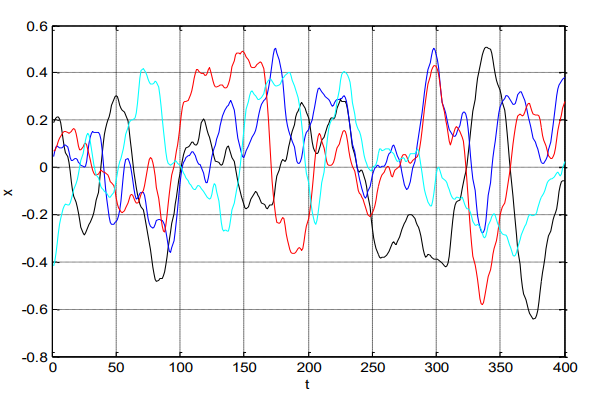
\includegraphics[width=0.82\textwidth]{viacero_realizacii_nahodneho_sumu.png}
  \caption{Množina realizácií náhodného procesu -- šum kovového rezistoru (každá krivka = jedno meranie).}
\end{figure}

\subsection{Stredná hodnota}

Stredná hodnota náhodného procesu v čase $t$ --- priemer cez všetky možné
hodnoty v danom okamihu, váhovaný hustotou $p(x,t)$:
\[
  a(t) = \int_{-\infty}^{+\infty} x \, p(x,t)\, dx
\]
kde $x$ je integrovaná premenná (možné hodnoty signálu) a $p(x,t)$ je hustota
rozdelenia v čase $t$. V praxi sa odhaduje ako aritmetický priemer $K$
realizácií v okamihu $t$:
\[
  \hat{a}(t) = \frac{1}{K}\sum_{k=1}^K x_k(t)
\]
kde $K$ je počet realizácií a $x_k(t)$ je hodnota $k$-tej realizácie v čase
$t$.

\subsection{Disperzia (rozptyl)}

Disperzia v čase $t$ --- priemerná kvadratická odchýlka hodnôt od strednej
hodnoty $a(t)$ v danom okamihu:
\[
  D(t) = \int_{-\infty}^{+\infty} \bigl[x - a(t)\bigr]^2 \, p(x,t)\, dx
\]
kde $x$ je integrovaná premenná (možné hodnoty signálu) a $a(t)$ je stredná
hodnota procesu v čase $t$. Čím väčšia $D(t)$, tým viac sú realizácie
v čase $t$ ,,roztrúsené'' okolo strednej hodnoty --- tým väčší výkon šumu.

\textbf{Smerodajná odchýlka} procesu: $\sigma(t) = \sqrt{D(t)}$

% ------------------------------------------------------------
\section{Autokorelačná funkcia (AKF)}
% ------------------------------------------------------------

AKF popisuje vzájomnú závislosť hodnôt signálu v dvoch rôznych časových
okamihoch --- hovorí, nakoľko ,,pamätá'' signál svoju minulosť. Pre
stacionárny náhodný proces závisí len od časového rozdielu $\tau = t_2 - t_1$,
nie od absolútneho času:
\[
  R(\tau) = E\{\xi(t) \cdot \xi(t+\tau)\}
\]
kde:
\begin{itemize}
  \item $\tau$ --- časové posunutie (oneskorenie) medzi dvoma okamihmi
        porovnávania [s]
  \item $\xi(t)$ --- hodnota náhodného procesu v čase $t$
  \item $\xi(t+\tau)$ --- hodnota toho istého procesu o $\tau$ neskôr
  \item $E\{\cdot\}$ --- operátor stredovania (priemer cez realizácie)
\end{itemize}

\textbf{Intuitívne:} pre $\tau = 0$ porovnávame signál sám so sebou ---
výsledok je maximálny. Pre rastúce $\tau$ sa hodnoty čoraz viac ,,rozídu''
a korelácia klesá. Pre biely šum klesne okamžite na nulu (žiadna pamäť), pre
hladký signál klesá pomaly.

\subsection{Vlastnosti AKF stacionárneho procesu}

\begin{itemize}
  \item \textbf{Maximum v $\tau = 0$}:
    \[
      R(0) = E\{\xi^2(t)\} = D + a^2
    \]
    čo je stredný výkon signálu. Pre nulový jednosmerný priebeh ($a = 0$):
    $R(0) = D = \sigma^2$
  \item \textbf{Párna funkcia}: $R(\tau) = R(-\tau)$ --- pohľad dopredu
        a dozadu v čase dáva rovnaký výsledok
  \item Pre veľké $\tau$ klesá k $a^2$ --- signál ,,zabudne'' svoju minulosť,
        ostane len prínos strednej hodnoty
  \item Disperzia $D$ v grafe AKF je výška poklesu od maxima $R(0)$
        k asymptote $a^2$, teda $D = R(0) - a^2$
  \item U procesov s nulovou strednou hodnotou ($a = 0$) má smerodajná
        odchýlka $\sigma$ význam efektívnej hodnoty signálu a platí
        $P = X_{ef}^2 = D = \sigma^2$ (výkon na záťaži 1\,$\Omega$)
\end{itemize}

\begin{figure}[H]
  \centering
  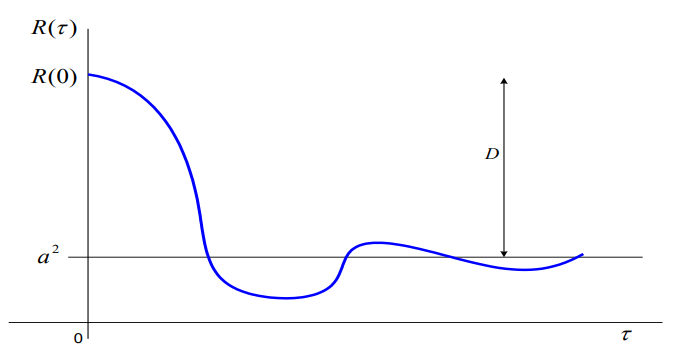
\includegraphics[width=0.82\textwidth]{tvar_autokorelacnej_funkcie.png}
  \caption{AKF stacionárneho náhodného signálu s vyznačenými hodnotami $R(0)$, $a^2$ a $D$.}
\end{figure}

% ------------------------------------------------------------
\section{Stacionarita}
% ------------------------------------------------------------

Náhodný proces je \textbf{stacionárny}, ak jeho štatistické charakteristiky
nezávisia od posunutia počiatku časovej osi --- sú rovnaké kdekoľvek v čase.
Formálne platí:
\[
  F(x,t) \to F(x), \qquad a(t) \to a, \qquad D(t) \to D
\]
\[
  p(x_1,x_2,t_1,t_2) \to p(x_1,x_2,\tau), \qquad \tau = t_2 - t_1
\]

\textbf{Predstav si to takto:} ak by si vystrihol ľubovoľný úsek záznamu
a vypočítal štatistiku, vždy dostaneš rovnaké výsledky. Typický príklad
stacionárneho procesu: tepelný šum rezistoru. Nestacionárny: zvuk záchranky,
ktorá mení frekvenciu --- jej štatistika sa mení s časom.

\begin{figure}[H]
  \centering
  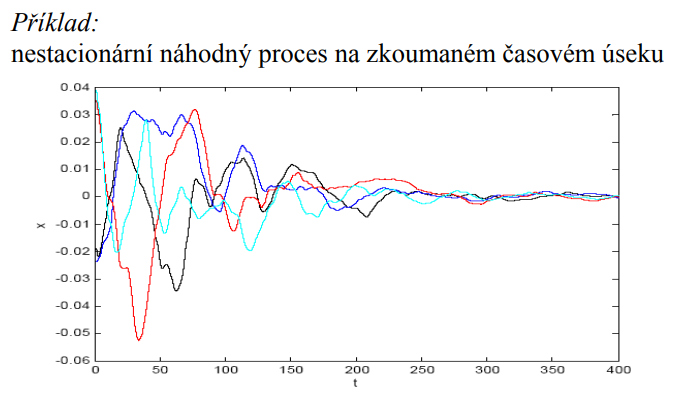
\includegraphics[width=0.82\textwidth]{priklad_nestacionarneho_nahodneho_procesu.png}
  \caption{Nestacionárny náhodný proces -- amplitúda realizácií sa mení s časom.}
\end{figure}

% ------------------------------------------------------------
\section{Ergodicita}
% ------------------------------------------------------------

Ergodický proces je stacionárny proces s ešte silnejšou vlastnosťou:
\textbf{všetky realizácie majú rovnaké štatistické vlastnosti} a stačí preto
skúmať jedinú (ľubovoľnú) realizáciu. Praktický dôsledok: časový priemer
vypočítaný z jednej dlhej realizácie = priemer cez realizácie v danom
okamihu.

Bez predpokladu ergodicity by sme pre odhad strednej hodnoty potrebovali
súbežne veľa meraní --- čo je v praxi často nemožné. Podmienkou je dostatočne
dlhý čas záznamu.

\textbf{Príklad:} šum rezistoru je ergodický --- jedno dlhé meranie stačí na
spoľahlivé určenie všetkých štatistík.

\begin{figure}[H]
  \centering
  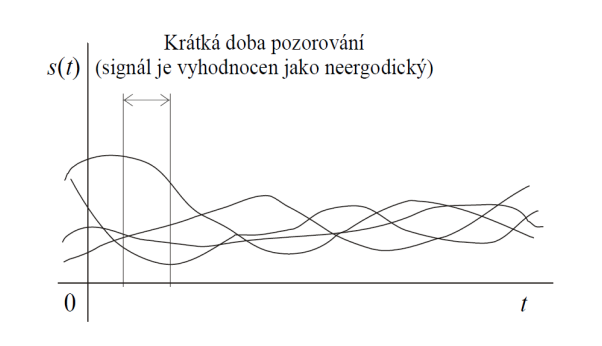
\includegraphics[width=0.82\textwidth]{priklad_ergodicity.png}
  \caption{Ergodicita -- pri krátkej dobe pozorovania sa realizácie zdajú rôzne; pri dostatočne dlhej sú štatisticky zhodné.}
\end{figure}

% ------------------------------------------------------------
\section{Spektrálna hustota výkonu $G(\omega)$}
% ------------------------------------------------------------

Kým AKF opisuje náhodný signál v čase, spektrálna hustota výkonu $G(\omega)$
opisuje, \textbf{ako je rozložený výkon signálu po frekvenciách} --- koľko
výkonu sa nachádza v každom frekvenčnom pásme. Funkcia je párna
($G(\omega) = G(-\omega)$) a nezáporná.

\textbf{Celkový stredný výkon} stacionárneho ergodického procesu:
\[
  P = \int_{-\infty}^{+\infty} G(\omega)\, d\omega
\]
kde $\omega$ je uhlová frekvencia [rad/s].

\textbf{Výkon v pásme} od $\omega_1$ do $\omega_2$:
\[
  P = 2\int_{\omega_1}^{\omega_2} G(\omega)\, d\omega
\]
(faktor 2 kvôli symetrii -- pre záporné frekvencie platí to isté).

\textbf{Biely šum} má konštantnú spektrálnu hustotu $G(\omega) = G$ pre
všetky frekvencie --- analogia k bielému svetlu, ktoré obsahuje všetky farby
rovnomerne. V reálnom svete neexistuje (mal by nekonečný výkon), ale je
dôležitý ako matematický model šumu.

\textbf{Meranie $G(\omega)$ v praxi} pásmovým filtrom so šírkou pásma $b$
a stredným kmitočtom $\omega_c$. Nameraný výkon $P(b, \omega_c)$ na výstupe
filtra dá:
\[
  G(\omega_c) \approx \frac{P(b,\, \omega_c)}{2b}
\]
kde $b$ je šírka pásma filtra [rad/s] a $P(b, \omega_c)$ je stredný výkon
nameraný na výstupe filtra. Čím užší filter, tým presnejší odhad spektra
v danom bode.

\begin{figure}[H]
  \centering
  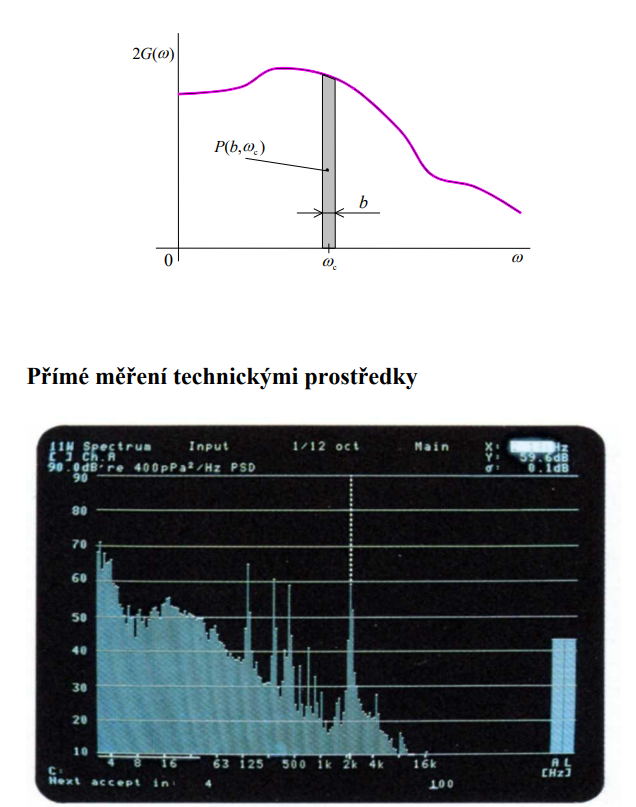
\includegraphics[width=0.82\textwidth]{graf_merania_priemyselného_hluku_a_schema_principu_merania.png}
  \caption{Schéma merania $G(\omega)$ pásmovým filtrom (hore) a reálne namerané spektrum priemyselného hluku (dole).}
\end{figure}

% ------------------------------------------------------------
\section{Typy šumov}
% ------------------------------------------------------------

Náhodné signály sa delia podľa rôznych kritérií:
\begin{itemize}
  \item \textbf{Stacionárny šum} --- spektrálne vlastnosti konštantné v čase
        (napr. hluk ventilátora, tepelný šum); oproti tomu \textbf{nestacionárny}
        --- meniace sa vlastnosti (siréna záchranky, štekat psa).
  \item \textbf{Bielý šum} --- rovnomerné spektrum;
        \textbf{farebný šum} --- získaný pásmovým filtrovaním bieleho
        (ružový, červený\ldots).
  \item \textbf{Aditivný šum} --- pripočítava sa k užitočnému signálu, nie je
        s ním korelovaný (napr. hluk pozadia pri nahrávaní mikrofónom).
  \item \textbf{Konvolučný šum} --- vzniká skreslením signálu v prenosovom
        kanáli, má väzbu na užitočný signál (napr. odrazy, dozvuk v miestnosti).
\end{itemize}

% ============================================================
% OKRUH 2
% 
\chapter{Lineárna filtrácia signálov -- filtre FIR a IIR}

% ------------------------------------------------------------
\section{Čo je filter a čo robí}
% ------------------------------------------------------------

Filter je systém, ktorý \textbf{selektívne prepúšťa určité frekvencie
a potláča iné}. Ideálny filter má pravoúhlu frekvenčnú charakteristiku
(dokonalé prepustenie v pásme, dokonalé potlačenie mimo neho); reálne filtre
majú pozvoľnejší prechod a istú mieru zvlnenia. Podľa prepúšťaného pásma
rozlišujeme:
\begin{itemize}
  \item \textbf{Dolná priepusť (DP)} --- prepúšťa nízke frekvencie
  \item \textbf{Horná priepusť (HP)} --- prepúšťa vysoké frekvencie
  \item \textbf{Pásmová priepusť (PP)} --- prepúšťa pásmo uprostred
  \item \textbf{Pásmová zádrž (PZ)} --- blokuje pásmo uprostred
\end{itemize}

% ------------------------------------------------------------
\section{Analógové filtre}
% ------------------------------------------------------------

Realizujú sa pasívnymi súčiastkami (R, C, L) alebo aktívne s operačným
zosilňovačom. Návrh prebieha v dvoch etapách.

\subsection{1. etapa -- signálová}

Výber prenosovej funkcie $H(p)$ vhodnou aproximáciou. Pre dolnú priepusť:
\[
  H(p) = \frac{K_0}{1 + k_1 P + k_2 P^2 + \ldots + k_N P^N}
\]
kde:
\begin{itemize}
  \item $K_0$ --- zosilnenie filtra na nulovom kmitočte [bezrozmerné]
  \item $N$ --- rád filtra; čím vyšší, tým strmší prechod medzi priepustným
        a zádrž\-ným pásmom
  \item $k_i$ ($i = 1 \ldots N$) --- koeficienty určujúce typ aproximácie,
        preberajú sa z tabuliek
  \item $P = j\omega/\omega_m$ --- normovaný komplexný kmitočet;
        $\omega_m$ je medzný (návrhový) kmitočet [rad/s]
\end{itemize}

Pre hornú priepusť sa prenosová funkcia získa zámenou $P \to 1/P$ (v obvode
to zodpovedá vzájomnej záméne kondenzátorov a rezistorov). Typ aproximácie
určuje správanie v priepustnom pásme:
\begin{itemize}
  \item \textbf{Butterworthova} --- maximálne plochá charakteristika,
        bez zvlnenia
  \item \textbf{Besselova} --- najlepšia linearita fázy (minimálne fázové
        skreslenie)
  \item \textbf{Čebyševova} --- strmší prechod za cenu zvlnenia v priepustnom
        pásme
\end{itemize}

\begin{figure}[H]
  \centering
  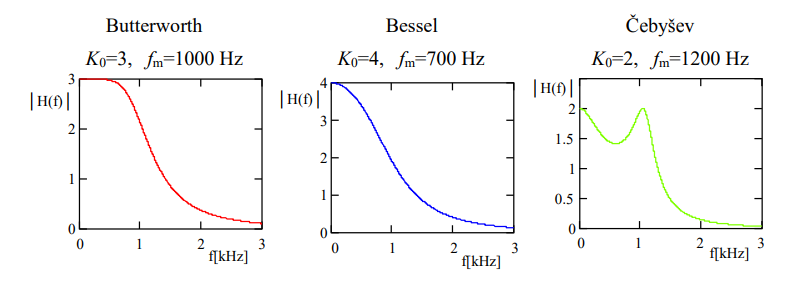
\includegraphics[width=0.82\textwidth]{porovnanie_modulovych_frek_char.png}
  \caption{Porovnanie modulových charakteristík dolnej priepuste -- Butterworth, Bessel, Čebyšev.}
\end{figure}

\subsection{2. etapa -- obvodová}

Na základe zvoleného zapojenia (napr. Sallenov-Keyov obvod) sa z koeficientov
$k_i$ vypočítajú konkrétne hodnoty súčiastok R a C.

% ------------------------------------------------------------
\section{Číslicové filtre -- FIR a IIR}
% ------------------------------------------------------------

Číslicové filtre pracujú s diskrétnymi vzorkami signálu. Výstup $y(n)$ je
určený konvolúciou vstupného signálu $x(n)$ s impulznou odozvou $h(k)$.
Podľa dĺžky impulznej odozvy rozlišujeme dve hlavné triedy.

\subsection{FIR -- Finite Impulse Response (konečná impulzná odozva)}

Výstup závisí len od $N$ posledných vstupných vzorkov:
\[
  y(n) = \sum_{k=0}^{N-1} h(k) \cdot x(n-k)
\]
kde:
\begin{itemize}
  \item $y(n)$ --- aktuálny výstupný vzorek
  \item $x(n-k)$ --- vstupné vzorky: $x(n)$ je aktuálny, $x(n-1)$ je
        o jeden krok starší, atď.
  \item $h(k)$ --- koeficienty filtra (= hodnoty impulznej odozvy
        v diskrétnom čase $k$)
  \item $N$ --- počet koeficientov (rád filtra $+ 1$)
\end{itemize}

Prenosová funkcia v $z$-oblasti:
\[
  H(z) = \sum_{k=0}^{N-1} h(k)\, z^{-k}
\]
kde $z^{-k}$ zodpovedá oneskoreniu o $k$ vzorkov. FIR nemá spätnú väzbu
--- každý výstupný vzorek závisí výlučne od vstupov.

\subsection{IIR -- Infinite Impulse Response (nekonečná impulzná odozva)}

Realizovaný rekurzívnou rovnicou (spätná väzba):
\[
  y(n) = \sum_{k=0}^{N} b_k \cdot x(n-k) \;-\; \sum_{k=1}^{M} a_k \cdot y(n-k)
\]
kde:
\begin{itemize}
  \item $b_k$ --- koeficienty priamej vetvy (váhy vstupných vzorkov $x$;
        $k = 0 \ldots N$)
  \item $a_k$ --- koeficienty spätnoväzbovej vetvy (váhy predchádzajúcich
        výstupov $y$; $k = 1 \ldots M$)
  \item $y(n-k)$ --- výstupné vzorky z minulosti, ktoré sa ,,vracajú'' späť
        do výpočtu
\end{itemize}

Prenosová funkcia:
\[
  H(z) = \frac{\displaystyle\sum_{k=0}^{N} b_k\, z^{-k}}
              {1 + \displaystyle\sum_{k=1}^{M} a_k\, z^{-k}}
\]

\textbf{Intuitívne:} vďaka spätnej väzbe ,,pamätá'' IIR filter svoju vlastnú
minulosť --- impulz na vstupe sa v systéme ,,odráža'' donekonečna (teoreticky),
preto nekonečná odozva. Toto mu dáva veľkú efektivitu: rovnako ostrú
frekvenčnú charakteristiku dosiahne s omnoho menej koeficientmi ako FIR.



% ------------------------------------------------------------
\section{Vlastnosti a porovnanie FIR vs IIR}
% ------------------------------------------------------------

\subsection*{FIR}
\begin{itemize}
  \item Vždy stabilný --- stabilita je garantovaná štruktúrou (žiadna spätná
        väzba nemôže spôsobiť rozkmitanie)
  \item Lineárna fázová charakteristika --- všetky frekvencie sú oneskorené
        o rovnakú dobu, takže tvar signálu nie je skreslený; kľúčové pre reč,
        EKG, dáta
  \item Pre ostrý prechod potrebuje vysoký rád (veľa koeficientov $N$)
        $\to$ dlhší výpočet, väčšia pamäť
  \item Rušivý impulz na vstupe ovplyvní výstup len po dobu $N$ vzorkov,
        potom zmizne
  \item Nemá analógový ekvivalent
\end{itemize}

\subsection*{IIR}
\begin{itemize}
  \item Môže byť nestabilný pri zle navrhnutých koeficientoch (spätná väzba
        môže spôsobiť nárast výstupu do nekonečna)
  \item Nelineárna fázová charakteristika --- rôzne frekvencie sú oneskorené
        rôzne dlho (fázové skreslenie)
  \item Nízky rád (typicky do 10) --- výpočtovo efektívny
  \item Krátky rušivý impulz môže prostredníctvom spätnej väzby trvale
        ovplyvniť výstup
  \item Analógové filtre sa dajú priamo previesť na IIR
        (metóda bilineárnej transformácie)
\end{itemize}

\noindent\textbf{Odporúčanie pre prax:}
\begin{itemize}
  \item \textbf{IIR} --- ak je hlavnou požiadavkou ostrá frekvenčná selekcia
        s čo najmenším počtom koeficientov
  \item \textbf{FIR} --- ak je dôležitá lineárna fáza, alebo počet
        koeficientov nie je problémom
\end{itemize}

% ------------------------------------------------------------
\section{Metódy návrhu číslicových filtrov v MATLABe}
% ------------------------------------------------------------

Všetky kmitočty použité v návrhu sú normované v rozsahu 0 až 1, kde 1
zodpovedá polovici vzorkovacieho kmitočtu $f_{vz}/2$. Napríklad pre medzný
kmitočet $f_m = 300$\,Hz a vzorkovací kmitočet 1000\,Hz (teda $f_{vz}/2 =
500$\,Hz) sa zadáva $W_p = 300/500 = 0{,}6$.

\textbf{Pre IIR} návrh prebieha v dvoch krokoch:

\noindent\textit{1. Výpočet rádu filtra $n$ a návrhového medzného kmitočtu $W_n$:}

\begin{center}
\begin{tabular}{ll}
  \toprule
  \textbf{Typ filtra} & \textbf{Funkcia} \\
  \midrule
  Butterworth        & \texttt{[n, Wn] = buttord(Wp, Ws, Rp, As)} \\
  Chebyshev I        & \texttt{[n, Wn] = cheb1ord(Wp, Ws, Rp, As)} \\
  Chebyshev II       & \texttt{[n, Wn] = cheb2ord(Wp, Ws, Rp, As)} \\
  Eliptický (Cauer)  & \texttt{[n, Wn] = ellipord(Wp, Ws, Rp, As)} \\
  \bottomrule
\end{tabular}
\end{center}

\noindent kde $W_p$ je normovaný medzný kmitočet v priepustnom pásme,
$W_s$ v zádrži (oba 0--1), $R_p$ je maximálne zvlnenie v priepustnom pásme
[dB], $A_s$ je minimálny útlm v zádrži [dB].

\noindent\textit{2. Výpočet koeficientov $b$ (čitateľ) a $a$ (menovateľ):}

\begin{center}
\begin{tabular}{ll}
  \toprule
  \textbf{Typ filtra} & \textbf{Funkcia} \\
  \midrule
  Butterworth        & \texttt{[b, a] = butter(n, Wn, options)} \\
  Chebyshev I        & \texttt{[b, a] = cheby1(n, Rp, Wn, options)} \\
  Chebyshev II       & \texttt{[b, a] = cheby2(n, As, Wn, options)} \\
  Eliptický          & \texttt{[b, a] = ellip(n, Rp, As, Wn, options)} \\
  \bottomrule
\end{tabular}
\end{center}

\noindent Filtrácia signálu $x$: \quad \texttt{y = filter(b, a, x)}

\textbf{Pre FIR}: najčastejšie metóda okien --- navrhnutá impulzná odozva
sa váhuje okienkovou funkciou (Hanning, Hamming, Kaiser) na potlačenie
vedľajších lalokov v zádrži. V MATLABe napr. \texttt{fir1}, \texttt{firpm}.



% ------------------------------------------------------------
\section{Spôsoby realizácie}
% ------------------------------------------------------------

Číslicové filtre sa realizujú:
\begin{itemize}
  \item \textbf{Softvérovo} --- výpočet rovnice $y(n)$ vzorku po vzorku
        v procesore alebo DSP čipe
  \item \textbf{Hardvérovo} --- obvody FPGA alebo ASIC implementujúce sieť
        násobiček a sčítavačov: pre FIR priama (transversálna) štruktúra,
        pre IIR rekurzívna štruktúra so spätnou väzbou
\end{itemize}

Vizualizácia vlastností filtra v MATLABe:
\begin{itemize}
  \item \texttt{freqz(b, a, K, fvz)} --- modulová a fázová frekvenčná
        charakteristika ($K$ bodov, vzorkovací kmitočet \texttt{fvz})
  \item \texttt{impz(b, a, N)} --- impulzná odozva ($N$ vzorkov)
  \item \texttt{zplane(b, a)} --- mapa núl a pólov v $z$-rovine
\end{itemize}

\begin{figure}[H]
  \centering
  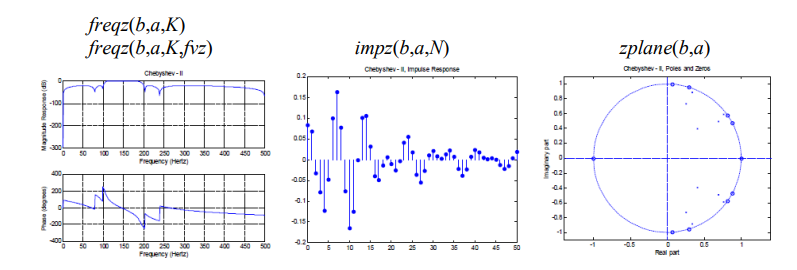
\includegraphics[width=0.82\textwidth]{frekvencna_char_impulzna_char_mapa_polov.png}
  \caption{Frekvenčná charakteristika, impulzná odozva a mapa pólov/núl číslicového filtra Chebyshev~II v MATLABe.}
\end{figure}

% ============================================================
% OKRUH 3
% ============================================================
\chapter{Lineárna predikcia signálu (LPC)}

% ------------------------------------------------------------
\section{Definícia lineárnej predikcie}
% ------------------------------------------------------------

Lineárna predikcia (LPC --- Linear Predictive Coding) spočíva v myšlienke,
že \textbf{aktuálny vzorek signálu vieme odhadnúť ako váhovanú sumu
predchádzajúcich vzorkov} toho istého signálu. Predikovaná hodnota $n$-tého
vzorka:
\[
  \hat{s}(n) = \sum_{m=1}^{M} a_m \cdot s(n-m)
\]
kde:
\begin{itemize}
  \item $\hat{s}(n)$ --- predikovaná (odhadnutá) hodnota vzorka s indexom $n$
  \item $s(n-m)$ --- skutočné hodnoty predchádzajúcich vzorkov: $s(n-1)$ je
        bezprostredne predchádzajúci, $s(n-2)$ je o dva kroky starší, atď.
  \item $a_m$ --- predikčné (LPC) koeficienty ($m = 1 \ldots M$); hovorí sa
        im aj ,,váhy''
  \item $M$ --- rád prediktora: koľko predchádzajúcich vzorkov použijeme
\end{itemize}

\textbf{Intuitívne:} je to podobné, ako keby si pri predpovedaní počasia
dnes ráno vychádzal z teplôt posledných $M$ dní --- každý deň má svoju váhu
$a_m$.

\textbf{Chyba predikcie} (reziduál) $e(n)$ --- rozdiel medzi skutočnou
a predikovanou hodnotou:
\[
  e(n) = s(n) - \hat{s}(n) = s(n) - \sum_{m=1}^{M} a_m \cdot s(n-m)
\]
kde $e(n)$ je chyba predikcie $n$-tého vzorka [rovnaká jednotka ako $s(n)$].

% ------------------------------------------------------------
\section{Výpočet koeficientov -- minimalizácia chyby}
% ------------------------------------------------------------

Cieľom LPC analýzy je nájsť koeficienty $a_m$ tak, aby bola celková
kvadratická chyba cez segment $N$ vzorkov minimálna:
\[
  Er = \sum_{n=1}^{N} e^2(n)
     = \sum_{n=1}^{N} \left[s(n) - \sum_{m=1}^{M} a_m \cdot s(n-m)\right]^2
\]
kde $Er$ je celková kvadratická chyba predikcie, $N$ je dĺžka spracovávaného
segmentu a $n$ je index vzorka v segmente.

Minimalizácia $Er$ parciálnymi deriváciami podľa každého $a_m$ vedie na
sústavu $M$ lineárnych rovníc --- \textbf{Yule-Walkerove rovnice}
v maticovom tvare:
\[
\begin{pmatrix}
  R(0)   & R(1)   & R(2)   & \cdots & R(M-1) \\
  R(1)   & R(0)   & R(1)   & \cdots & R(M-2) \\
  \vdots &        &        & \ddots & \vdots \\
  R(M-1) & R(M-2) & R(M-3) & \cdots & R(0)
\end{pmatrix}
\begin{pmatrix} a_1 \\ a_2 \\ \vdots \\ a_M \end{pmatrix}
=
\begin{pmatrix} R(1) \\ R(2) \\ \vdots \\ R(M) \end{pmatrix}
\]
kde $R(k)$ je autokorelačná funkcia segmentu signálu pri oneskorení $k$
--- teda miera podobnosti signálu so sebou samým posunutým o $k$ vzorkov.
Matica je Toeplitzová (symetrická, každá diagonála má rovnaké hodnoty), čo
umožňuje efektívne riešenie Levinsonovým-Durbinovým algoritmom.

\textbf{Prakticky:} čím je signál periodickejší (napr. znelá samohláska),
tým väčšia $R(k)$ pre $k = $ perióda, tým lepšie koeficienty dokážu
predpovedať nasledujúce vzorky. Šumové (neznelé) úseky (napr.\ hláska ,,s'')
majú $R(k) \approx 0$ pre $k > 0$ --- predikcia funguje oveľa horšie.

\begin{figure}[H]
  \centering
  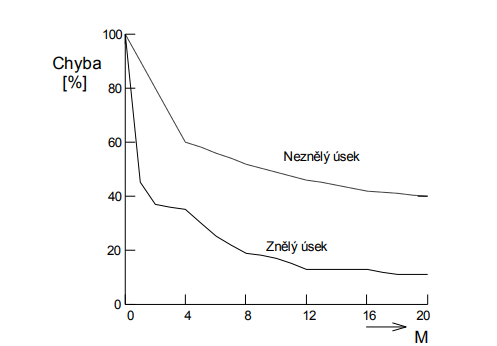
\includegraphics[width=0.82\textwidth]{zavislost_chyby_zneleho_a_nezneleho_useku.png}
  \caption{Závislosť chyby predikcie na počte koeficientov $M$ pre znelý a neznelý úsek reči.}
\end{figure}

% ------------------------------------------------------------
\section{Využitie pre reštauráciu signálu}
% ------------------------------------------------------------

Ak poznáme koeficienty $a_m$ a máme k dispozícii predchádzajúce vzorky,
vieme dopočítať chýbajúci alebo poškodený vzorek:
\[
  \hat{s}(n) = \sum_{m=1}^{M} a_m \cdot s(n-m)
\]
Namiesto predikcie budúcich vzorkov rekonštruujeme chýbajúce. Funguje tým
lepšie, čím je signál viac ,,predvídateľný'' --- teda pre hladké, kváziperiodické
úseky (samohlásky, hudba). Pre šumové úseky je reštaurácia menej presná.

% ------------------------------------------------------------
\section{Využitie pre spektrálnu analýzu -- LPC spektrum}
% ------------------------------------------------------------

Z predikčných koeficientov $a_m$ možno pomocou $z$-transformácie vypočítať
\textbf{LPC spektrum}:
\[
  LS(f) = \left|\frac{1}{1 - \displaystyle\sum_{m=1}^{M} a_m \cdot
  z^{-m}}\right|^2_{\!\!z\,=\,\exp(j2\pi f/f_{vz})}
\]
kde:
\begin{itemize}
  \item $f$ --- frekvencia spektra (nezávislá premenná) [Hz],
        v rozsahu $0$ až $f_{vz}/2$
  \item $f_{vz}$ --- vzorkovací kmitočet signálu [Hz]
  \item $a_m$ --- predikčné koeficienty ($m = 1 \ldots M$)
  \item $z^{-m}$ --- oneskorenie o $m$ vzorkov v $z$-oblasti; dosadením
        $z = e^{j2\pi f/f_{vz}}$ prechádzame do frekvenčnej oblasti
\end{itemize}

LPC spektrum má tvar \textbf{vyhladenej obálky FFT spektra} --- potláča
detailné kolísanie a zvýrazňuje spektrálne vrcholy. Miera vyhlazenia závisí
od $M$: nízke $M$ $\to$ hrubá aproximácia (len celkový sklon), vyššie $M$
$\to$ jemnejší tvar s viditeľnými vrcholmi. Pre reč typicky $M = 10$--$16$
koeficientov.

\begin{figure}[H]
  \centering
  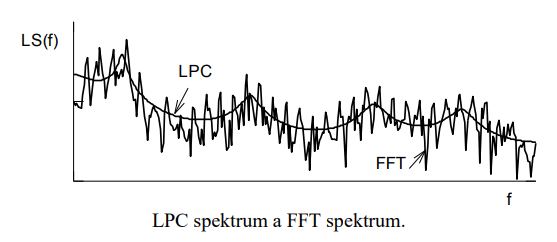
\includegraphics[width=0.82\textwidth]{porovnanie_LPC_a_FFT_spektra.png}
  \caption{LPC spektrum (vyhladená obálka) vs.\ FFT spektrum pre ten istý segment reči.}
\end{figure}

\begin{figure}[H]
  \centering
  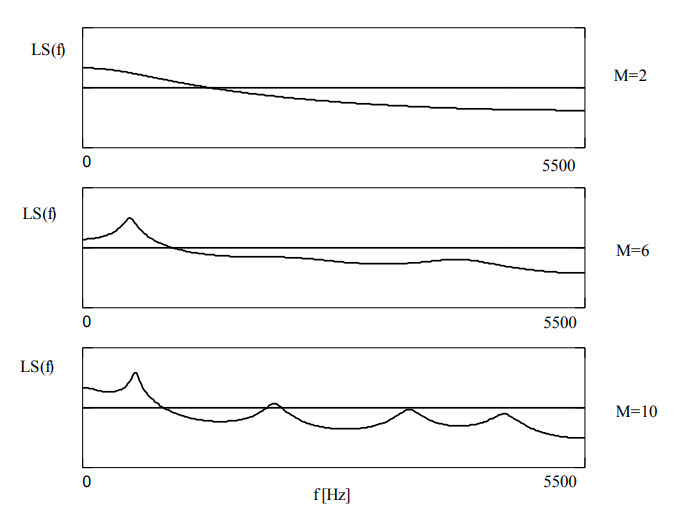
\includegraphics[width=0.82\textwidth]{vplyv_poctu_koeficientov_na_LPC.png}
  \caption{Vplyv počtu koeficientov $M$ na tvar LPC spektra ($M = 2, 6, 10$).}
\end{figure}

Lokálne maximá LPC spektra zodpovedajú \textbf{formantovým kmitočtom} ---
rezonančným frekvenciám vokálneho traktu pri tvorbe danej hlásky. Tieto
možno určiť priamo z pólov $z$-transformácie (korene rovnice
$1 - \sum_{m=1}^{M} a_m \cdot z^{-m} = 0$), čo nevyžaduje ani vykresľovanie
spektra.

% ------------------------------------------------------------
\section{Význam pre rozpoznávanie reči}
% ------------------------------------------------------------

LPC je kľúčová metóda v spracovaní reči z viacerých dôvodov:

\textbf{1. Model hlasového traktu.} Reč vzniká excitáciou (hlasivky
generujú periodický sled impulzov pre znelé hlásky, alebo šum pre neznelé)
filtrovanou vokálnym traktom. LPC model tento filter priamo parametrizuje
--- koeficienty $a_m$ charakterizujú tvar vokálneho traktu pre danú hlásku
v danom časovom okamihu. Tá istá hláska ,,a'' bude mať u rôznych ľudí rôzne
spektrum, ale LPC koeficienty zachytia tvar spektra nezávisle od výšky
hlasu.

\textbf{2. Kompaktná reprezentácia.} Namiesto tisícok vzoriek v 20\,ms
segmente stačí 10--16 predikčných koeficientov. To dramaticky redukuje objem
dát --- podstatné pre kódovanie a prenos reči.

\textbf{3. Príznakové vektory pre klasifikátor.} LPC koeficienty (alebo
z nich odvodené cepstrálne koeficienty LPCC) tvoria príznakové vektory pre
klasifikátory (HMM, DTW, neurónové siete). Každý segment reči je opísaný
vektorom $(a_1, a_2, \ldots, a_M)$ a rozpoznávač hľadá, ku ktorej triede
(hláske, slovu) je tento vektor najbližšie.

\textbf{4. Rozlíšenie znelosti.} Znelé úseky sa predikujú s malou chybou
$e(n)$, neznelé s veľkou. Energia reziduálu je preto sama o sebe príznakom
znelosti --- priamo využiteľné pri segmentácii reči.


\subsection*{Zhrnutie -- význam a využitie metódy LPC}

\begin{itemize}
  \item \textbf{Predpovídání budoucích vzorků} --- na základe koeficientov $a_m$
        a predchádzajúcich vzorkov možno odhadnúť nasledujúce vzorky signálu
        v časovom priebehu (využitie pri kompresii, reštaurácii, kódovaní reči)
  \item \textbf{Výpočet spektra (modulového)} --- z koeficientov $a_m$ sa
        priamo vypočíta vyhladené LPC spektrum $LS(f)$, ktoré reprezentuje
        spektrálnu obálku signálu a polohu formantov
  \item \textbf{Využití LPC koeficientů ke klasifikaci signálů} --- koeficienty
        $a_m$ (alebo z nich odvodené cepstrálne koeficienty LPCC) tvoria
        príznakové vektory pre klasifikátory rozpoznávania reči (HMM, DTW,
        neurónové siete)
\end{itemize}

% ============================================================
%\end{document}
	% !TeX root = statnicaEKT.tex
\part{BPC-DE1 - Digitální elektronika 1}
\begin{huge}
	Otázky:
	\newline
\end{huge}
\begin{enumerate}
	\item Otázka - Logická hradla. Postuláty a zákony Booleovy algebry. 
	\item Otázka - Klopné obvody. Typy, vlastnosti, zapojení a realizace. 
	\item Otázka - Čítače. Typy, vlastnosti, zapojení a realizace. 
\end{enumerate}
%%%%%%%%%%%%%%%%%%%%%%%%%%%%%%%%%%%%%%%%%%%%%%%%%%%%%
\chapter{Logické hradlá, postuláty a zákony Boolovej algebry}
%%%%%%%%%%%%%%%%%%%%%%%%%%%%%%%%%%%%%%%%%%%%%%%%%%%%%

\section{Čo sú logické hradlá?}

Digitálne obvody pracujú len s dvoma hodnotami: \textbf{0} (nízke napätie, ``nepravda'') a \textbf{1} (vysoké napätie, ``pravda''). \textbf{Logické hradlo} je najjednoduchší stavebný blok -- elektronický obvod, ktorý vykoná jednu logickú operáciu a výsledok dá na výstup.

\begin{figure}[H]
    \centering
    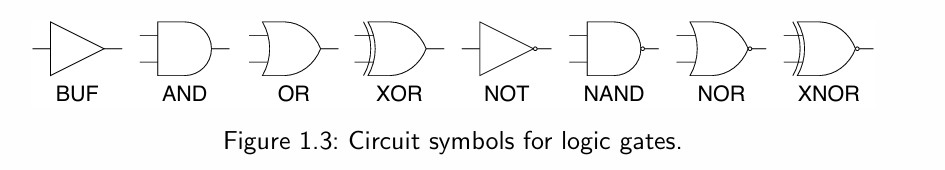
\includegraphics[width=0.85\textwidth]{Obrazky/Obrazky_DE1/fig_hradla_znacky.jpg}
    \caption{Schematické značky základných logických hradiel. Zľava: BUF (sledovač -- kopíruje vstup na výstup), AND (logický súčin), OR (logický súčet), XOR (exkluzívny súčet), NOT (invertor), NAND, NOR a XNOR. \textbf{Krúžok na výstupe vždy znamená negáciu.}}
    \label{fig:hradla_znacky}
\end{figure}

\section{Základné logické hradlá}

\subsection{AND -- logický súčin (``A zároveň'')}

AND hovorí: výstup je 1, len keď sú \textbf{oba} vstupy 1. Ako dva spínače zapojené za sebou -- prúd tečie, len keď sú zavreté oba.

\begin{minipage}{0.52\textwidth}
Výstup $y = a \cdot b$ je 1 iba ak $a=1$ \textbf{a zároveň} $b=1$.
\end{minipage}
\hfill
\begin{minipage}{0.44\textwidth}
\begin{center}
\begin{tabular}{cc|c}
\toprule
$a$ & $b$ & $y$ \\
\midrule
0 & 0 & 0 \\
0 & 1 & 0 \\
1 & 0 & 0 \\
1 & 1 & \textbf{1} \\
\bottomrule
\end{tabular}
\end{center}
\end{minipage}

\subsection{OR -- logický súčet (``alebo'')}

OR hovorí: výstup je 1, keď je aspoň jeden vstup 1. Ako dva spínače zapojené paralelne -- stačí zavrieť jeden.

\begin{minipage}{0.52\textwidth}
Výstup $y = a + b$ je 1 ak $a=1$ \textbf{alebo} $b=1$ (alebo oboje).
\end{minipage}
\hfill
\begin{minipage}{0.44\textwidth}
\begin{center}
\begin{tabular}{cc|c}
\toprule
$a$ & $b$ & $y$ \\
\midrule
0 & 0 & 0 \\
0 & 1 & \textbf{1} \\
1 & 0 & \textbf{1} \\
1 & 1 & \textbf{1} \\
\bottomrule
\end{tabular}
\end{center}
\end{minipage}

\subsection{NOT -- invertor (negácia)}

NOT obráti hodnotu: z 0 urobí 1 a z 1 urobí 0. Ako prepínač ``zapnuté/vypnuté''.

\subsection{XOR -- exkluzívny súčet (``jeden alebo druhý, ale nie obaja'')}

XOR hovorí: výstup je 1, ak sa vstupy \textbf{líšia}. Praktické využitie: detekcia rozdielu, sčítavanie bitov.

\begin{minipage}{0.52\textwidth}
Výstup $y = a \oplus b$ je 1, ak sú vstupy \textbf{rôzne}.
\end{minipage}
\hfill
\begin{minipage}{0.44\textwidth}
\begin{center}
\begin{tabular}{cc|c}
\toprule
$a$ & $b$ & $y$ \\
\midrule
0 & 0 & 0 \\
0 & 1 & \textbf{1} \\
1 & 0 & \textbf{1} \\
1 & 1 & 0 \\
\bottomrule
\end{tabular}
\end{center}
\end{minipage}

\subsection{NAND a NOR -- univerzálne hradlá}

NAND = AND s negovaným výstupom. NOR = OR s negovaným výstupom.

Prečo sú také dôležité? Sú to \textbf{univerzálne hradlá} -- z jedného typu (len z NANDov alebo len z NORov) možno zostrojiť \textit{akúkoľvek} logickú funkciu, teda aj AND, OR alebo NOT. V praxi sa celé procesory vyrábajú výhradne z NAND hradiel -- sú najjednoduchšie na výrobu v CMOS technológii.

\textbf{NAND ako NOT:} stačí spojiť oba vstupy dokopy: NAND($a$, $a$) = NOT($a$). Dve hradlá za sebou dajú AND.

\section{Boolova algebra -- pravidlá pre prácu s logickými výrazmi}

Boolova algebra je sada matematických pravidiel, ktoré popisujú správanie logických premenných. Umožňuje \textbf{zjednodušovať zložité výrazy} -- a tým zjednodušovať a šetriť hradlá v obvode.

\textbf{Vplyv konštánt -- čo sa stane, keď na vstup privedieme pevnú 0 alebo 1:}
\begin{center}
\begin{tabular}{ll}
$0 + a = a$ & OR s nulou: nula nič nepridá, výsledok závisí len na $a$ \\
$1 + a = 1$ & OR s jednotkou: jednotka vždy vyhrá, výsledok je vždy 1 \\
$1 \cdot a = a$ & AND s jednotkou: jednotka nič nezmení \\
$0 \cdot a = 0$ & AND s nulou: nula vždy vyhrá, výsledok je vždy 0 \\
$a + a = a$ & OR sám so sebou: nič nové \\
$a \cdot a = a$ & AND sám so sebou: nič nové \\
\end{tabular}
\end{center}

\textbf{Negácia:}
\begin{center}
\begin{tabular}{ll}
$a + \bar{a} = 1$ & premenná OR jej opak: vždy jeden z nich je 1, výsledok vždy 1 \\
$a \cdot \bar{a} = 0$ & premenná AND jej opak: nemôžu byť obe 1, výsledok vždy 0 \\
$\bar{\bar{a}} = a$ & dvojitá negácia sa ruší \\
\end{tabular}
\end{center}

\textbf{Komutatívnosť} -- na poradí nezáleží: $a + b = b + a$. Rovnako ako pri sčítavaní čísel.

\textbf{Asociatívnosť} -- závorky možno preusporiadať: $(a + b) + c = a + (b + c)$.

\textbf{Distributívnosť} -- roznásobovanie závoriek: $a \cdot (b + c) = a\cdot b + a\cdot c$.

\textbf{Absorpcia (pohltenie)} -- zjednodušenie, ktoré nie je na prvý pohľad zrejmé: $a + a \cdot b = a$. Prečo? Ak $a=1$, je výsledok 1 bez ohľadu na $b$. Ak $a=0$, potom $a \cdot b = 0$ tiež, výsledok je 0. Výsledok závisí len na $a$ -- $b$ je zbytočné.

\section{De Morganove zákony -- najdôležitejšie pravidlá}

De Morganove zákony hovoria, ako ``pretlačiť negáciu dovnútra'' výrazu. Sú kľúčové pre zjednodušovanie obvodov a pre pochopenie, prečo NAND a NOR sú ekvivalentné s inými kombináciami hradiel.

\medskip
\textbf{Zákon 1:} $\overline{a \cdot b} = \bar{a} + \bar{b}$\quad (NAND = OR s negovanými vstupmi)

Slovne: ``Nie je pravda, že A aj B'' = ``Buď nie je A, alebo nie je B.''

Príklad zo života: ``Nezatvoril som dvere \textbf{a} okno'' = ``Buď som nezatvoril dvere, \textbf{alebo} som nezatvoril okno.''

\medskip
\textbf{Zákon 2:} $\overline{a + b} = \bar{a} \cdot \bar{b}$\quad (NOR = AND s negovanými vstupmi)

Slovne: ``Nie je pravda, že A alebo B'' = ``Ani A, ani B.''

Príklad zo života: ``Nesvieti lampa \textbf{ani} televízor'' = ``Nesvieti lampa \textbf{a zároveň} nesvieti televízor.''

\medskip
\textbf{Praktický dôsledok:} Každý AND možno nahradiť NORom s negovanými vstupmi a naopak. To znamená, že celý obvod možno realizovať len z jedného typu hradla.

\textbf{Princíp duality:} Každý platný výraz Boolovej algebry zostane platný, keď vymeníme AND$\leftrightarrow$OR a $0\leftrightarrow 1$ všade. De Morganove zákony sú presne takým párom.

\section{Minimalizácia logických funkcií}

Každú logickú funkciu možno zapísať ako \textbf{tabuľku pravdivosti} -- pre každú kombináciu vstupov je uvedený výstup. Z tabuľky zostrojíme obvod, ale ten býva zbytočne zložitý. Minimalizácia hľadá ekvivalentný, ale jednoduchší výraz.

\textbf{SoP (Sum of Products)} -- súčet súčinov: pre každý riadok kde je výstup 1 napíšeme súčin všetkých vstupov (mintermový term), potom ich sčítame (OR). Priamočiare, ale výraz nemusí byť najjednoduchší.

\textbf{PoS (Product of Sums)} -- súčin súčtov: podobný postup, ale vychádzame z riadkov kde je výstup 0.

\textbf{Karnaughova mapa (K-mapa):} grafická metóda zjednodušovania, praktická pre funkcie do 4 premenných. Tabuľka pravdivosti sa prepíše do špeciálnej mriežky, kde susedné políčka sa líšia práve v jednom bite. Skupiny susedných jednotiek zodpovedajú zjednodušeným súčinom -- čím väčšia skupina ($1, 2, 4, 8$ políčok), tým jednoduchší výsledný výraz.

\newpage

%%%%%%%%%%%%%%%%%%%%%%%%%%%%%%%%%%%%%%%%%%%%%%%%%%%%%
\chapter{Klopné obvody -- typy, vlastnosti, zapojenie a realizácia}
%%%%%%%%%%%%%%%%%%%%%%%%%%%%%%%%%%%%%%%%%%%%%%%%%%%%%

\section{Prečo potrebujeme klopné obvody?}

Logické hradlá sú \textbf{kombinačné} -- výstup závisí len na aktuálnych vstupoch, bez pamäte. Ale procesor potrebuje \textbf{pamätať si} hodnoty -- výsledky výpočtov, aktuálny stav systému, obsah registrov. Na to slúžia \textbf{klopné obvody} -- majú dva stabilné stavy (0 a 1) a samy si udržia svoj stav, kým ho niekto nezmení.

Analógia: klopný obvod je ako svetelný vypínač -- zostane v stave ``zapnuté'' alebo ``vypnuté'', kým ho neprepnete.

\textbf{Dva základné typy:}
\begin{itemize}
    \item \textbf{Latch (asynchrónny):} reaguje okamžite na \textbf{úroveň} riadiaceho signálu. Kým je EN aktívny, vstup prechádza priamo na výstup (``transparentný'').
    \item \textbf{Flip-flop (synchrónny):} reaguje presne na \textbf{hranu} hodinového signálu (prechod 0$\rightarrow$1 alebo 1$\rightarrow$0). Mimo hrany je vstup zmrazený -- výstup sa nemení.
\end{itemize}

\section{S-R Latch -- najjednoduchší pamäťový prvok}

S-R latch má dva vstupy: \textbf{S} (Set -- nastav $Q$ na 1) a \textbf{R} (Reset -- nastav $Q$ na 0). Výstupy $Q$ a $\bar{Q}$ sú vždy vzájomne opačné (jeden je 0, druhý 1).

\subsection{Realizácia pomocou NOR hradiel}

\begin{figure}[H]
    \centering
    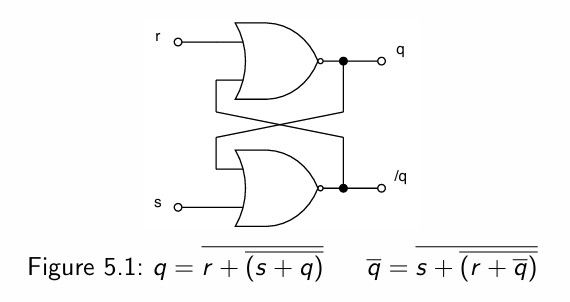
\includegraphics[width=0.45\textwidth]{Obrazky/Obrazky_DE1/fig_sr_latch_nor.jpg}
    \caption{S-R latch z dvoch NOR hradiel. Kľúčom je \textbf{spätná väzba} -- výstup každého hradla je privedený na vstup druhého. Vďaka tomu sa obvod ``udrží'' v nastavenom stave aj po uvoľnení vstupu -- to je princíp pamäte.}
    \label{fig:sr_latch_nor}
\end{figure}

Ako si obvod pamätá: nastavíme $S=1$ a $Q$ sa prepne na 1. Spätná väzba potom zabezpečí, že $Q=1$ drží výstup druhého NOR hradla na 0, a to zase drží $Q=1$ -- slučka sa ``uzamkla''. Po uvoľnení $S$ zostane $Q=1$.

\begin{center}
\begin{tabular}{cc|cc|l}
\toprule
$S$ & $R$ & $Q$ & $\bar{Q}$ & Čo sa deje \\
\midrule
0 & 0 & $Q$ & $\bar{Q}$ & \textbf{Pamäť} -- stav sa nemení \\
1 & 0 & 1 & 0 & \textbf{Set} -- nastav $Q$ na 1 \\
0 & 1 & 0 & 1 & \textbf{Reset} -- nastav $Q$ na 0 \\
1 & 1 & ? & ? & \textbf{ZAKÁZANÉ!} -- výstupy nie sú opačné \\
\bottomrule
\end{tabular}
\end{center}

\begin{figure}[H]
    \centering
    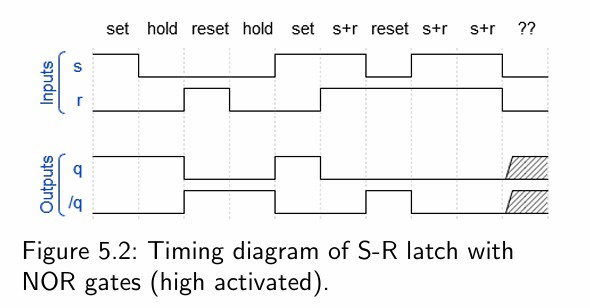
\includegraphics[width=0.55\textwidth]{Obrazky/Obrazky_DE1/fig_sr_latch_nor_timing.jpg}
    \caption{Časový diagram S-R latchu. $S=1$ prepne $Q$ na 1. $R=1$ vráti $Q$ na 0. Šrafovaná oblasť je zakázaný stav ($S=R=1$) -- pri návrate z tohto stavu nevieme, v akom stave sa obvod ustáli (\textbf{metastabilita}).}
    \label{fig:sr_latch_nor_timing}
\end{figure}

\textbf{Zakázaný stav a metastabilita:} Ak sú oba vstupy $S=R=1$ a potom oba naraz prejdú na 0, obvod nevie, do akého stavu skočiť. Ocitne sa v \textbf{metastabilnom stave} -- výstup osciluje alebo sa ustáli na neurčitej hodnote po dobu desiatok nanosekúnd. To môže pokaziť funkciu celého systému.

\subsection{Realizácia pomocou NAND hradiel}

Funguje rovnako, ale aktívna úroveň je opačná -- obvod reaguje na \textbf{nízku} (log. 0) úroveň vstupov $\bar{S}$ a $\bar{R}$.

\begin{figure}[H]
    \centering
    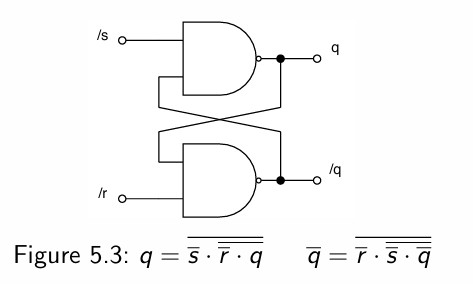
\includegraphics[width=0.45\textwidth]{Obrazky/Obrazky_DE1/fig_sr_latch_nand.jpg}
    \caption{S-R latch z dvoch NAND hradiel. Oproti NOR verzii sú vstupné úrovne invertované -- pokojový stav (pamäť) je $\bar{S}=\bar{R}=1$, zakázaný stav je $\bar{S}=\bar{R}=0$.}
    \label{fig:sr_latch_nand}
\end{figure}

\section{Gated S-R Latch -- pridáme povoľovací vstup}

Základný S-R latch reaguje ihneď -- kedykoľvek sa zmení $S$ alebo $R$, výstup okamžite reaguje. V praxi potrebujeme riadiť, \textbf{kedy} smie obvod reagovať. Gated latch pridáva vstup \textbf{EN (Enable)}:

\begin{itemize}
    \item $EN = 1$: obvod je ``odomknutý'' -- sleduje vstupy normálne
    \item $EN = 0$: obvod je ``zamknutý'' -- ignoruje vstupy, drží posledný stav
\end{itemize}

\begin{figure}[H]
    \centering
    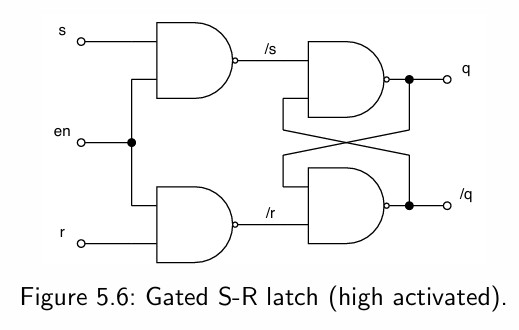
\includegraphics[width=0.50\textwidth]{Obrazky/Obrazky_DE1/fig_gated_sr_latch.jpg}
    \caption{Gated S-R latch. Pridané AND hradlá fungujú ako ``brána'' -- prepustia $S$ a $R$ len vtedy, keď $EN=1$. Pri $EN=0$ sú oba vstupy AND hradiel nulové a vnútorný SR latch drží svoj stav.}
    \label{fig:gated_sr_latch}
\end{figure}

\begin{figure}[H]
    \centering
    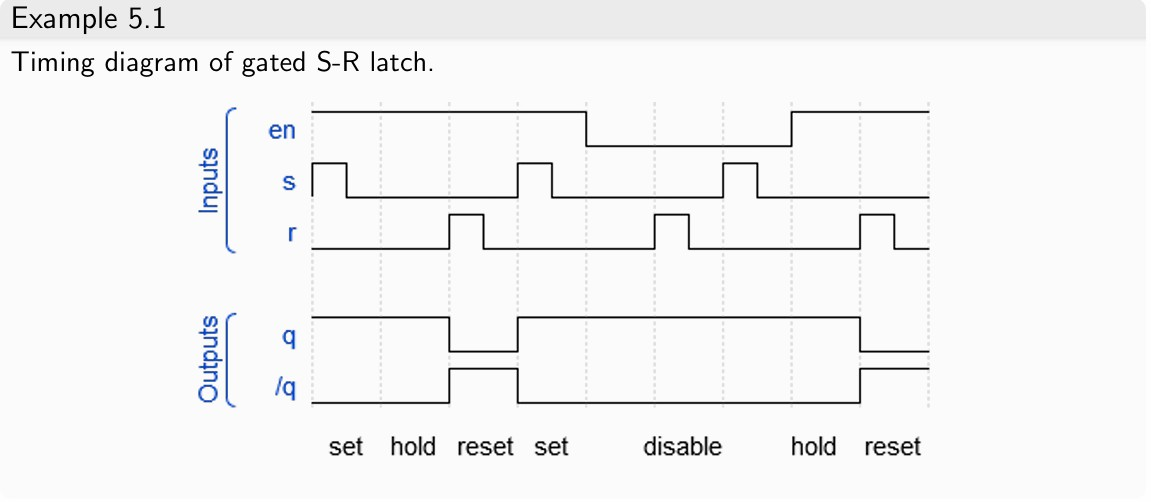
\includegraphics[width=0.60\textwidth]{Obrazky/Obrazky_DE1/fig_gated_sr_timing.jpg}
    \caption{Časový diagram Gated S-R latchu -- vidíme postupne štyri situácie: set (nastavenie), hold (udržanie), reset (vynulovanie) a disable ($EN=0$, obvod ignoruje vstupy a drží posledný stav).}
    \label{fig:gated_sr_timing}
\end{figure}

\section{D Latch -- transparentný latch}

S-R latch má zakázaný stav ($S=R=1$). Ako ho odstrániť? Jednoducho: pridáme invertor tak, aby $R$ bolo vždy opakom $S$. Tým $S$ a $R$ nikdy nemôžu byť oba 1 naraz. Vstup premenujeme na \textbf{D (Data)}.

\begin{figure}[H]
    \centering
    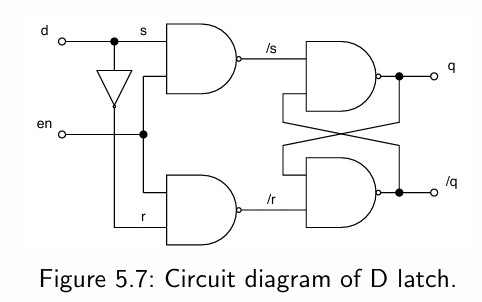
\includegraphics[width=0.50\textwidth]{Obrazky/Obrazky_DE1/fig_d_latch.jpg}
    \caption{D latch. Invertor zaručuje $R = \bar{D}$ -- zakázaný stav SR latchu nemôže nastať. Pri $EN=1$ výstup $Q$ okamžite sleduje vstup $D$ (``transparentný'' režim). Na zostupnej hrane EN sa aktuálna hodnota $D$ uzamkne.}
    \label{fig:d_latch}
\end{figure}

\begin{figure}[H]
    \centering
    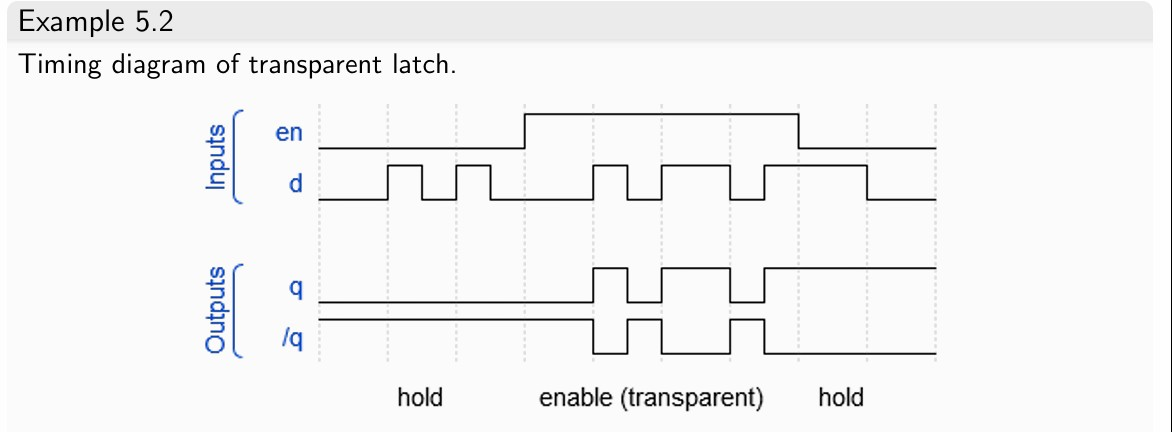
\includegraphics[width=0.60\textwidth]{Obrazky/Obrazky_DE1/fig_d_latch_timing.jpg}
    \caption{Časový diagram D latchu. Pri $EN=1$ výstup $Q$ okamžite kopíruje vstup $D$. Na zostupnej hrane $EN$ sa aktuálna hodnota ``uzamkne'' a $Q$ ju drží aj po deaktivácii -- to je princíp latchu.}
    \label{fig:d_latch_timing}
\end{figure}

\textbf{Problém D latchu:} ak sa $D$ zmení v čase, keď $EN=1$, okamžite to prejde na výstup. V synchrónnych systémoch chceme, aby ku zmene došlo \textbf{presne na hrane hodín} -- nie kedykoľvek. To rieši flip-flop.

\section{D Flip-flop -- reaguje len na hranu hodín}

D flip-flop rieši problém D latchu tým, že \textbf{dva D latche zapojí za sebou} s opačnými hodinami -- tzv. \textbf{Master-Slave štruktúra}.

\begin{figure}[H]
    \centering
    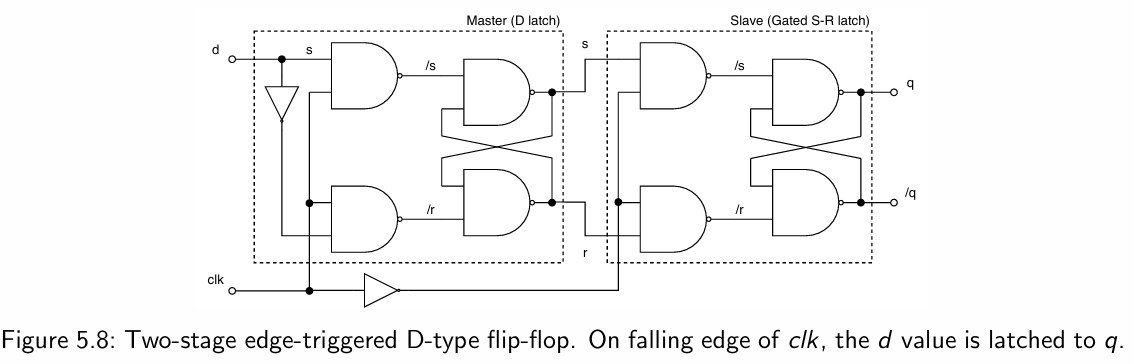
\includegraphics[width=0.80\textwidth]{Obrazky/Obrazky_DE1/fig_d_ff_master_slave.jpg}
    \caption{Master-Slave D flip-flop z dvoch latchov. Master (vľavo) sa otvorí pri $CLK=1$ a zachytí $D$. Slave (vpravo) sa otvorí pri $CLK=0$ (invertované hodiny) a prepustí hodnotu na výstup $Q$. Nikdy nie sú oba otvorené naraz -- výstup sa zmení len raz za periódu, presne na hrane CLK.}
    \label{fig:d_ff_master_slave}
\end{figure}

\textbf{Ako to funguje krok po kroku:}
\begin{enumerate}
    \item $CLK$ prejde na 1 $\Rightarrow$ Master sa otvorí a zachytí aktuálne $D$; Slave je zamknutý
    \item $CLK$ prejde na 0 $\Rightarrow$ Master sa uzavrie (uzamkne zachytenú hodnotu); Slave sa otvorí a prepustí túto hodnotu na výstup $Q$
\end{enumerate}

Výsledok: $Q$ sa zmení vždy presne na \textbf{zostupnej hrane CLK} -- nie skôr, nie neskôr. Charakteristická rovnica: $Q_{n+1} = D$ (po hrane je výstup rovný vstupu pred hranou).

\begin{figure}[H]
    \centering
    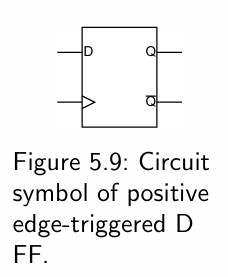
\includegraphics[width=0.22\textwidth]{Obrazky/Obrazky_DE1/fig_d_ff_symbol.jpg}
    \caption{Schematická značka D flip-flopu. Trojuholník na vstupe CLK znamená ``reaguje na hranu''. Verzia bez trojuholníka = latch (reaguje na úroveň).}
    \label{fig:d_ff_symbol}
\end{figure}

\begin{figure}[H]
    \centering
    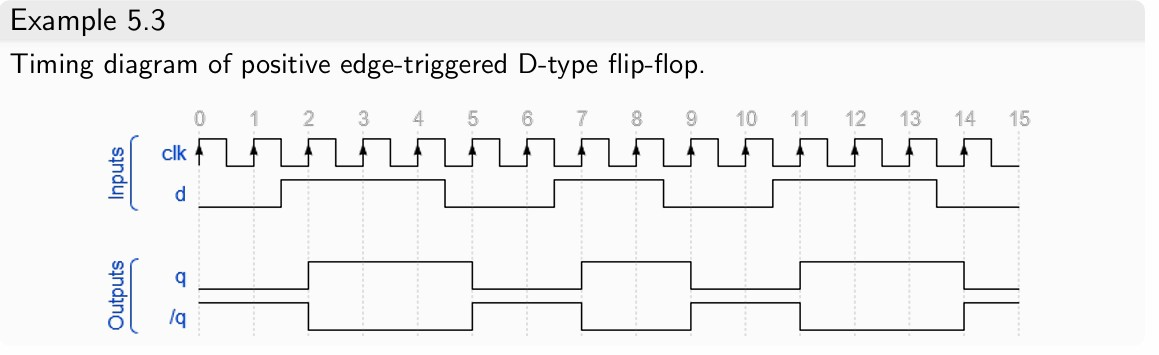
\includegraphics[width=0.75\textwidth]{Obrazky/Obrazky_DE1/fig_d_ff_timing.jpg}
    \caption{Časový diagram D flip-flopu s nábežnou hranou. $Q$ preberá hodnotu $D$ vždy len v okamžiku nábežnej hrany CLK ($\uparrow$). Medzi hranami zostáva $Q$ stabilné bez ohľadu na zmeny $D$.}
    \label{fig:d_ff_timing}
\end{figure}

\section{JK Flip-flop -- zakázaný stav sa stane užitočným}

JK flip-flop vychádza zo SR flip-flopu, ale zakázaný stav ($J=K=1$) mení na užitočnú funkciu: \textbf{Toggle} -- prehoď výstup na opačnú hodnotu. Dosiahne to spätnými väzbami z $Q$ a $\bar{Q}$ do vstupov.

\begin{figure}[H]
    \centering
    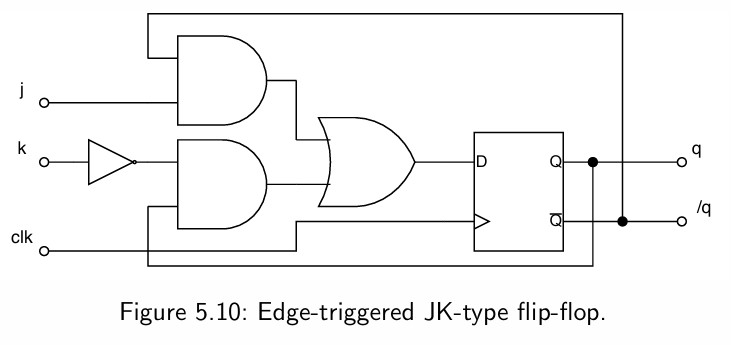
\includegraphics[width=0.70\textwidth]{Obrazky/Obrazky_DE1/fig_jk_ff.jpg}
    \caption{JK flip-flop. Spätné väzby z výstupov $Q$ a $\bar{Q}$ do vstupných AND hradiel zabránia zakázanému stavu -- kombinácia $J=K=1$ spôsobí toggle namiesto neurčitého stavu. Ak je $Q=1$, vstup cez AND pre $J$ je blokovaný hodnotou $\bar{Q}=0$, takže sa môže len resetovať (a naopak).}
    \label{fig:jk_ff}
\end{figure}

\begin{center}
\begin{tabular}{cc|c|l}
\toprule
$J$ & $K$ & $Q_{n+1}$ & Čo sa deje \\
\midrule
0 & 0 & $Q_n$       & \textbf{Pamäť} -- nič sa nemení \\
0 & 1 & 0           & \textbf{Reset} -- vynuluj \\
1 & 0 & 1           & \textbf{Set} -- nastav na 1 \\
1 & 1 & $\bar{Q}_n$ & \textbf{Toggle} -- prehoď! \\
\bottomrule
\end{tabular}
\end{center}

\begin{figure}[H]
    \centering
    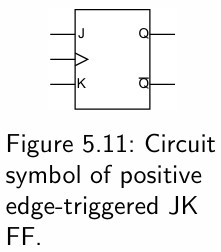
\includegraphics[width=0.22\textwidth]{Obrazky/Obrazky_DE1/fig_jk_ff_symbol.jpg}
    \caption{Schematická značka JK flip-flopu. $J$ zodpovedá Set, $K$ zodpovedá Reset -- navyše $J=K=1$ prehodí výstup.}
    \label{fig:jk_ff_symbol}
\end{figure}

\textbf{Excitačná tabuľka} -- aké $J$ a $K$ potrebujem, aby sa výstup prepol z $Q_n$ na $Q_{n+1}$? Potrebujeme ju pri návrhu sekvenčných obvodov (stavových automatov):

\begin{center}
\begin{tabular}{cc|cc}
\toprule
$Q_n$ & $Q_{n+1}$ & $J$ & $K$ \\
\midrule
0 & 0 & 0 & $\times$ (jedno čo) \\
0 & 1 & 1 & $\times$ \\
1 & 0 & $\times$ & 1 \\
1 & 1 & $\times$ & 0 \\
\bottomrule
\end{tabular}
\end{center}

\section{T Flip-flop -- delič frekvencie}

T flip-flop vznikne z JK flip-flopu jednoducho: spojíme oba vstupy $J$ a $K$ do jedného vstupu $T$. Má len dve funkcie:

\begin{center}
\begin{tabular}{c|c|l}
\toprule
$T$ & $Q_{n+1}$ & Čo sa deje \\
\midrule
0 & $Q_n$       & \textbf{Pamäť} -- drž stav \\
1 & $\bar{Q}_n$ & \textbf{Toggle} -- prehoď \\
\bottomrule
\end{tabular}
\end{center}

\begin{figure}[H]
    \centering
    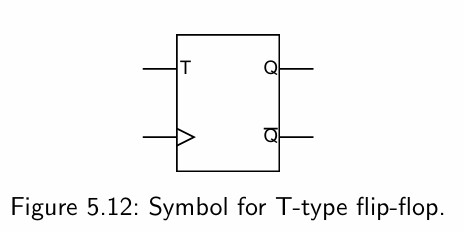
\includegraphics[width=0.22\textwidth]{Obrazky/Obrazky_DE1/fig_t_ff_symbol.jpg}
    \caption{Schematická značka T flip-flopu. Pri trvale $T=1$ sa výstup prehadzuje na každej hrane CLK -- výstupná frekvencia je presne \textbf{polovičná} oproti CLK.}
    \label{fig:t_ff_symbol}
\end{figure}

\textbf{Kľúčová vlastnosť:} T flip-flop s $T=1$ delí frekvenciu hodinového signálu presne dvoma. Kaskáda $n$ T flip-flopov delí frekvenciu $2^n$-krát. To je základ binárnych čítačov.

\section{Časové parametre -- kedy musí byť vstup stabilný?}

Flip-flop zachytí hodnotu $D$ presne na hrane CLK. Ale elektronické obvody nie sú ideálne -- potrebujú čas na spracovanie. Preto musí byť $D$ stabilné po určitú dobu \textit{okolo} hrany CLK.

\begin{figure}[H]
    \centering
    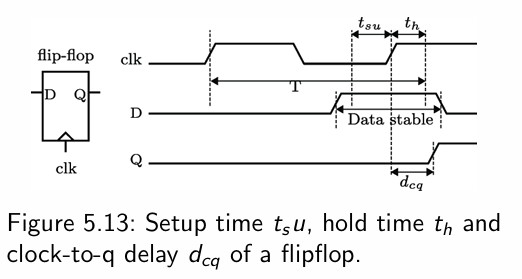
\includegraphics[width=0.80\textwidth]{Obrazky/Obrazky_DE1/fig_setup_hold.jpg}
    \caption{Časové parametre flip-flopu. \textbf{Setup time $t_{su}$}: $D$ musí byť stabilné najmenej $t_{su}$ \textit{pred} hranou CLK. \textbf{Hold time $t_h$}: $D$ musí zostať stabilné najmenej $t_h$ \textit{po} hrane CLK. \textbf{Clock-to-Q $d_{cq}$}: výstup $Q$ sa zmení až za $d_{cq}$ po hrane -- flip-flop potrebuje čas na ``prepnutie''.}
    \label{fig:setup_hold}
\end{figure}

\textbf{Čo sa stane pri porušení?} Flip-flop sa dostane do \textbf{metastabilného stavu} -- nezachytí ani 0 ani 1, výstup sa chvíľu nevyrovná a spôsobuje chyby v celom systéme.

\textbf{Maximálna hodinová frekvencia} -- hodiny môžu tikať len tak rýchlo, ako rýchlo sa stihne propagovať signál z výstupu cez kombinačnú logiku späť na vstup. Platí: $f_{max} = 1 / (d_{cq} + t_{comb} + t_{su})$.

\section{Posuvné registre}

Posuvný register je rad D flip-flopov zapojených za sebou -- výstup $Q$ jedného ide na vstup $D$ ďalšieho, všetky na spoločnom CLK. Pri každom takte sa dáta posunú o jeden krok doprava.

Použitie:
\begin{itemize}
    \item \textbf{SIPO} (Serial In, Parallel Out): prijať dáta sériovo (bit po bite) a čítať ich naraz paralelne -- napríklad čítanie dát zo SPI obvodu
    \item \textbf{PISO} (Parallel In, Serial Out): prijať dáta paralelne a odosielať ich sériovo
    \item Oneskorenie signálu o presne $n$ taktov
\end{itemize}

\newpage

%%%%%%%%%%%%%%%%%%%%%%%%%%%%%%%%%%%%%%%%%%%%%%%%%%%%%
\chapter{Čítače -- typy, vlastnosti, zapojenie a realizácia}
%%%%%%%%%%%%%%%%%%%%%%%%%%%%%%%%%%%%%%%%%%%%%%%%%%%%%

\section{Čo je čítač a na čo slúži?}

Čítač je sekvenčný obvod, ktorý \textbf{počíta hodinové impulzy}. Jeho výstup je binárne číslo, ktoré sa s každým taktom zvyšuje (alebo znižuje). Čítače sú základom časovačov, frekvenčných deličov, adresovania pamäte a mnohých ďalších aplikácií.

Kľúčové pojmy:
\begin{itemize}
    \item $n$ flip-flopov $\Rightarrow$ maximálne $2^n$ rôznych stavov
    \item \textbf{Modulus (MOD)}: koľko stavov čítač prejde pred návratom na začiatok. MOD-8 prejde stavmi 0, 1, 2, \ldots, 7 a vráti sa.
\end{itemize}

\section{Asynchrónny čítač (Ripple counter)}

\textbf{Myšlienka:} T flip-flop s $T=1$ delí frekvenciu dvoma -- výstup sa prehadzuje každý takt. Zapojme za sebou viac T flip-flopov, kde každý taktuje ten nasledujúci. Každý stupeň delí frekvenciu predchádzajúceho dvoma a výsledkom je binárny čítač!

\begin{figure}[H]
    \centering
    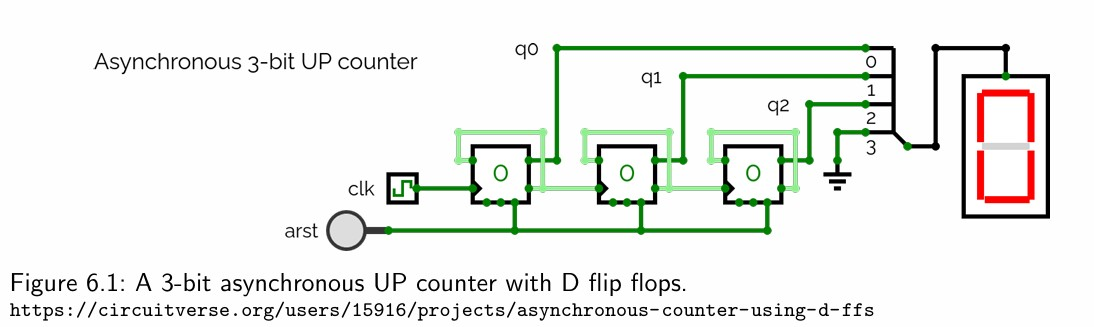
\includegraphics[width=0.75\textwidth]{Obrazky/Obrazky_DE1/fig_async_counter.jpg}
    \caption{3-bitový asynchrónny UP čítač. Každý D flip-flop má $D$ spojené s $\bar{Q}$ (toggle). Výstup $\bar{Q}$ každého stupňa taktuje stupeň nasledujúci. $Q_0$ sa mení každý takt, $Q_1$ každý druhý, $Q_2$ každý štvrtý -- dokopy tvoria binárny čítač 0--7.}
    \label{fig:async_counter}
\end{figure}

\textbf{Výhoda:} extrémne jednoduché zapojenie, žiadna kombinačná logika.

\begin{figure}[H]
    \centering
    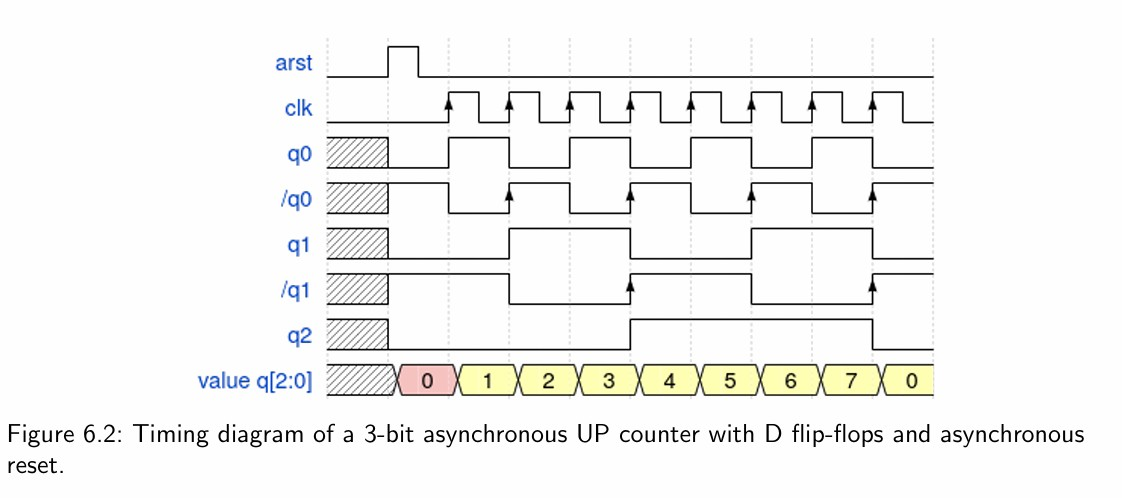
\includegraphics[width=0.75\textwidth]{Obrazky/Obrazky_DE1/fig_async_counter_timing.jpg}
    \caption{Časový diagram asynchrónneho čítača. Pri prechode 3$\rightarrow$4 (binárne $011 \to 100$) sa menia všetky tri bity -- ale nie naraz. Vidíme krátke falošné (glitch) hodnoty (010, 000) kým sa všetko ustáli. To je hlavná nevýhoda asynchrónneho čítača.}
    \label{fig:async_counter_timing}
\end{figure}

\subsection{Ripple efekt -- hlavná nevýhoda}

Prečo sa volá ``ripple'' (vlna)? Pretože zmena sa šíri ako vlna -- prvý flip-flop sa prepne, potom druhý, potom tretí\ldots Každý pridá svoje oneskorenie $t_{FF}$.

\textbf{Pri prechode 011 $\rightarrow$ 100} sa menia všetky tri bity, ale postupne -- v medziobdobí sa na výstupe krátko objavia \textbf{falošné (glitch) hodnoty}. To spôsobuje problémy, ak výstup čítača riadi iné obvody.

\textbf{Maximálna frekvencia} klesá s počtom bitov: s každým pridaným flip-flopom narastá oneskorenie o $t_{FF}$, teda $f_{max} = 1/(n \cdot t_{FF} + t_{su})$.

\section{Synchrónny čítač}

\textbf{Riešenie ripple efektu:} zapojíme všetky flip-flopy na \textbf{spoločný CLK} signál. Všetky sa prepnú \textbf{v rovnaký okamih} -- glitche zmiznú.

Nevýhoda: musíme pridať kombinačnú logiku, ktorá každému flip-flopu povie, či sa má v tomto takte prepnúť alebo nie.

\begin{figure}[H]
    \centering
    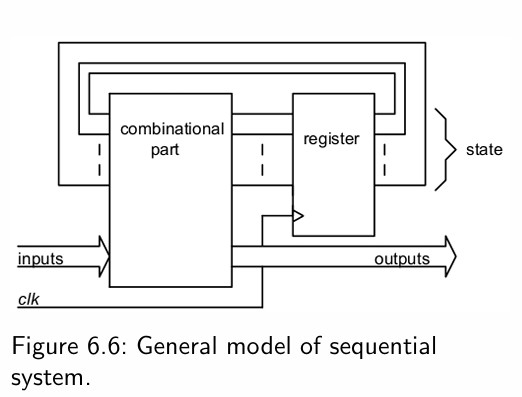
\includegraphics[width=0.50\textwidth]{Obrazky/Obrazky_DE1/fig_sync_model.jpg}
    \caption{Všeobecný model synchrónneho sekvenčného systému. Kombinačná logika na základe aktuálneho stavu vypočíta, čo bude v nasledujúcom takte. Register (flip-flopy) si všetko zapamätá na hrane CLK. Spätná väzba uzatvára slučku.}
    \label{fig:sync_model}
\end{figure}

\textbf{Pravidlo pre T flip-flopy:} bit $Q_i$ sa má prepnúť (toggle), iba keď \textbf{všetky nižšie bity sú jednotky} -- vtedy pretekajú a spôsobia prenos do vyššieho bitu.

\begin{itemize}
    \item $Q_0$: prepne sa vždy ($T_0 = 1$)
    \item $Q_1$: prepne sa, keď $Q_0 = 1$
    \item $Q_2$: prepne sa, keď $Q_1 = 1$ a $Q_0 = 1$
\end{itemize}

\textbf{Dva typy propagácie prenosu:}
\begin{itemize}
    \item \textbf{Parallel carry}: jedno veľké AND hradlo sleduje všetky nižšie bity naraz -- rýchle, ale AND hradlo rastie s každým bitom
    \item \textbf{Ripple carry}: prenos sa šíri postupne cez kaskádu 2-vstupových AND hradiel -- úspornejšie, ale pomalšie
\end{itemize}

\section{LFSR -- pseudonáhodný generátor}

\textbf{LFSR (Linear Feedback Shift Register)} je posuvný register, ktorého vstup je XOR kombinácia vybraných výstupov (tzv. ``taps''). Výsledkom je \textbf{pseudonáhodná sekvencia} -- postupnosť, ktorá vyzerá náhodne, ale je deterministická a opakuje sa.

\begin{figure}[H]
    \centering
    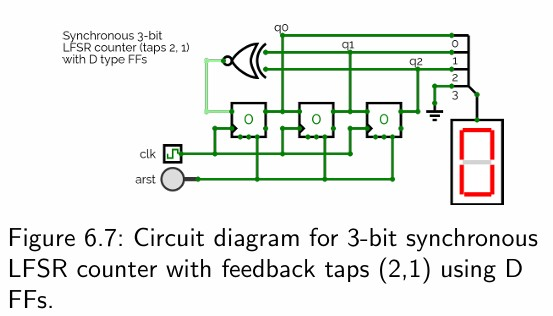
\includegraphics[width=0.65\textwidth]{Obrazky/Obrazky_DE1/fig_lfsr.jpg}
    \caption{3-bitový LFSR. Dáta sa posúvajú doprava. Spätná väzba z $Q_2$ a $Q_1$ cez XOR generuje nový bit na vstupe $D_0$. Stav $000$ sa nikdy neobjaví (XOR samých núl dá nulu -- zacyklenie). Sekvencia prechádza $2^3 - 1 = 7$ rôznymi stavmi.}
    \label{fig:lfsr}
\end{figure}

\textbf{Prečo $2^n - 1$ a nie $2^n$ stavov?} Stav samých núl je ``mŕtvy'' -- XOR samých núl dá opäť nulu, LFSR by sa nikdy nedostal z tohto stavu. Preto ho preskočíme (alebo použijeme XNOR a preskočíme stav samých jednotiek).

\textbf{Použitie:} generovanie testovacích sekvencií, kryptografia (stream ciphers), prenosové protokoly (scrambling), Wi-Fi pseudonáhodné sekvencie.

\section{Porovnanie: asynchrónny vs. synchrónny čítač}

\begin{center}
\begin{tabular}{lll}
\toprule
\textbf{Vlastnosť} & \textbf{Asynchrónny} & \textbf{Synchrónny} \\
\midrule
Taktovanie flip-flopov & Každý iným signálom   & Všetky rovnakým CLK \\
Glitche na výstupe     & Áno (ripple efekt)    & Nie \\
Kombinačná logika      & Žiadna                & AND hradlá pre prenos \\
Maximálna frekvencia   & Klesá s počtom bitov  & Nezávisí na počte bitov \\
Zložitosť návrhu       & Veľmi jednoduchý      & Stredne zložitý \\
Použitie               & Delič frekvencie, RTC & Procesory, FPGA, DSP \\
\bottomrule
\end{tabular}
\end{center}
	% !TeX root = statnicaEKT.tex
\part{BPC-DE2 - Digitální elektronika 2}
\begin{huge}
	Otázky:
	\newline
\end{huge}
\begin{enumerate}
	\item Otázka - Reprezentace čísel pomocí signed/unsigned fixed-point, floating-point, binární, dekadická a hexadecimální soustava. 
	\item Otázka - Struktura a funkce čítačů/časovačů. Popis a využití přetečení, komparace, módy PWM. 
	\item Otázka - Sériová komunikace UART a I2C. Popis, struktura rámců a komunikačních protokolů, použití a srovnání.
	
\end{enumerate}
%%%%%%%%%%%%%%%%%%%%%%%%%%%%%%%%%%%%%%%%%%%%%%%%%%%
\chapter{Reprezentácia čísel: fixed-point, floating-point, číselné sústavy}
%%%%%%%%%%%%%%%%%%%%%%%%%%%%%%%%%%%%%%%%%%%%%%%%%%%

\section{Prečo rôzne číselné sústavy?}

Človek prirodzene používa \textbf{dekadickú sústavu} (základ 10, číslice 0--9). Digitálne obvody pracujú iba s napätiami ``nízke'' a ``vysoké'' -- prirodzene teda používajú \textbf{binárnu sústavu} (základ 2, číslice 0 a 1). \textbf{Hexadecimálna sústava} (základ 16, číslice 0--9 a a--f) slúži ako skratka pre zápis binárnych hodnôt -- jeden hex symbol zastúpi vždy presne 4 bity.

Prefixový zápis: \texttt{0b} pre binárne (napr. \texttt{0b100} = 4), \texttt{0x} pre hexadecimálne (napr. \texttt{0x1F} = 31).

\begin{center}
\begin{tabular}{ccc}
\toprule
\textbf{Dekadická} & \textbf{Binárna} & \textbf{Hexadecimálna} \\
\midrule
0  & 0000 & 0 \\
9  & 1001 & 9 \\
10 & 1010 & a \\
15 & 1111 & f \\
16 & 0001\,0000 & 10 \\
\bottomrule
\end{tabular}
\end{center}

\section{Váhovanie bitov -- ako čítať binárne číslo}

Každý bit na určitej pozícii má svoju \textbf{váhu} -- hodnotu, ktorú pridáva k celkovému číslu. Pozície sa počítajú sprava od 0, váha pozície $i$ je $2^i$.

Príklad: \texttt{1011} = $1{\cdot}8 + 0{\cdot}4 + 1{\cdot}2 + 1{\cdot}1 = 11_{10}$.

Bit s najvyššou váhou (úplne vľavo) = \textbf{MSB} (Most Significant Bit). Bit s najnižšou váhou (úplne vpravo) = \textbf{LSB} (Least Significant Bit).

Pre čísla s desatinnou časťou: bity napravo od rádovej čiarky majú záporné mocniny ($2^{-1} = 0{,}5$; $2^{-2} = 0{,}25$; atď.).

\subsection{Prevod dekadicky $\to$ binárne}

\textbf{Celá časť:} opakované delenie dvoma, zvyšky sú výsledné bity od LSB k MSB.

Príklad: $25 \div 2 = 12$ zb. \textbf{1}; $12 \div 2 = 6$ zb. \textbf{0}; $6 \div 2 = 3$ zb. \textbf{0}; $3 \div 2 = 1$ zb. \textbf{1}; $1 \div 2 = 0$ zb. \textbf{1}. Čítame zvyšky zdola nahor: $25_{10} = \texttt{11001}_2$.

\textbf{Desatinná časť:} opakované násobenie dvoma, celé časti sú výsledné bity za rádovou čiarkou.

Príklad: $0{,}375 \times 2 = \mathbf{0}{,}75$; $0{,}75 \times 2 = \mathbf{1}{,}5$; $0{,}5 \times 2 = \mathbf{1}{,}0$ $\Rightarrow$ $0{,}375_{10} = \texttt{0.011}_2$.

\subsection{Prevod hexadecimálne $\leftrightarrow$ binárne}

Kľúčové pravidlo: \textbf{každý hex symbol = presne 4 bity}. Prevod prebieha symbol po symbole bez nutnosti iterácií.

$\texttt{0x6F} = \underbrace{0110}_{6}\underbrace{1111}_{F} = \texttt{0110\,1111}_2$\quad a naopak\quad $\texttt{1100\,1010}_2 = \underbrace{1100}_{C}\underbrace{1010}_{A} = \texttt{0xCA}$

\section{BCD -- každá číslica zvlášť}

V \textbf{BCD (Binary Coded Decimal)} sa každá dekadická číslica kóduje samostatne štyrmi bitmi. Číslo 25 v BCD: $\underbrace{0010}_{2}\underbrace{0101}_{5}$ = \texttt{0010\,0101} -- to je iné číslo ako binárne \texttt{11001}! BCD sa používa napríklad v kalkulačkách a digitálnych displejoch, kde je potrebné ľahko zobrazovať jednotlivé číslice.

\section{Unsigned vs. Signed -- kladné alebo záporné čísla?}

Procesor nevie, či číslo v registri je kladné alebo záporné -- to závisí od toho, ako ho \textbf{interpretujeme}.

\textbf{Unsigned} (neznamienkový): všetky bity sú váhové. 8 bitov pojme čísla 0 až 255.

\textbf{Signed} (znamienkový, dvojkový doplnok): MSB má \textit{zápornú} váhu. 8 bitov pojme čísla -128 až +127. Rovnaký bitový vzor \texttt{1111\,1110} znamená 254 (unsigned) alebo -2 (signed) -- záleží na kontexte!

\begin{center}
\begin{tabular}{cccc}
\toprule
\textbf{Počet bitov} & \textbf{Kombinácií} & \textbf{Unsigned} & \textbf{Signed} \\
\midrule
8  & 256     & 0 až 255     & -128 až 127 \\
16 & 65\,536 & 0 až 65\,535 & -32\,768 až 32\,767 \\
\bottomrule
\end{tabular}
\end{center}

\textbf{Dvojkový doplnok -- ako previesť kladné číslo na záporné:}
\begin{enumerate}
    \item Invertuj všetky bity (jedničkový doplnok)
    \item Pripočítaj 1
\end{enumerate}

Príklad: $+2 = \texttt{0000\,0010}$ $\xrightarrow{\text{inverzia}}$ \texttt{1111\,1101} $\xrightarrow{+1}$ $-2 = \texttt{1111\,1110}$.

\textbf{Prečo dvojkový doplnok?} Pretože sčítanie funguje normálne: $+2 + (-2) = \texttt{0000\,0010} + \texttt{1111\,1110} = \texttt{0000\,0000}$ (carry sa zahodí). Procesor nemusí mať zvláštny obvod pre odčítanie!

\textbf{Pretečenie (wrap-around):} 8-bitový unsigned systém je modulo 256 -- po pripočítaní 1 k 255 dostaneme 0. Ako ciferník hodín: po 12 príde opäť 1.

\section{Fixed-point -- pevná rádová čiarka}

Fixed-point čísla fungujú ako celé čísla, ale my si \textbf{zapamätáme, kde je rádová čiarka}. Notácia \textbf{Q formát}: $Q_{m.n}$ znamená $m$ bitov pre celú časť a $n$ bitov pre desatinnú časť.

Príklad Q4.4 (8 bitov celkovo): bity majú váhy $8, 4, 2, 1 \,.\, 0{,}5,\ 0{,}25,\ 0{,}125,\ 0{,}0625$.

Najmenší rozlíšiteľný krok = $2^{-n}$ (pre Q4.4 = 0,0625). Presnosť je konštantná v celom rozsahu.

\textbf{Bitový posun ako násobenie/delenie:} posun doľava o 1 = násobenie 2; posun doprava o 1 = delenie 2. Veľmi rýchla operácia v hardvéri!

\textbf{Použitie:} DSP, spracovanie zvuku, embedded systémy bez FPU -- rýchle a jednoduché na hardvér.

\section{Floating-point -- pohyblivá rádová čiarka}

Fixed-point má problém: pre čísla s veľkým dynamickým rozsahom (od veľmi malých po veľmi veľké) buď strácame presnosť alebo rozsah. Riešenie: \textbf{pohyblivá rádová čiarka} -- číslo je vyjadrené ako mantisa $\times 2^{\text{exponent}}$, podobne ako vedecký zápis ($1{,}23 \times 10^{-5}$).

Štandard \textbf{IEEE 754} definuje, ako sú tieto čísla uložené v pamäti. Číslo má tri časti:
\begin{itemize}
    \item \textbf{Znamienko S} (1 bit): 0 = kladné, 1 = záporné
    \item \textbf{Exponent} (8 bitov pre SP): poloha rádovej čiarky -- ako veľmi číslo ``naskálovať''
    \item \textbf{Mantisa / frac} (23 bitov pre SP): presné číslice čísla
\end{itemize}

\begin{center}
\begin{tabular}{lccc}
\toprule
\textbf{Formát} & \textbf{Bitov celkovo} & \textbf{Exponent} & \textbf{Mantisa} \\
\midrule
Single (SP, \texttt{float}) & 32 & 8 bitov & 23 bitov \\
Double (DP, \texttt{double}) & 64 & 11 bitov & 52 bitov \\
\bottomrule
\end{tabular}
\end{center}

\textbf{Normalizácia:} mantisa sa vždy zapíše v tvare $1.xxx$ (binárne) -- rádová čiarka sa posunie za prvú jednotku. Počiatočná jednotka sa ani neukladá (je tam vždy) -- to ušetrí 1 bit presnosti.

\textbf{Bias exponentu:} aby neboli potrebné záporné exponenty, pripočíta sa pevná hodnota (bias = 127 pre SP). Uložený exponent 130 znamená skutočný exponent $130 - 127 = +3$.

\textbf{Špeciálne hodnoty:} exponent samých jednotiek = infinity alebo NaN (Not a Number). Exponent samých núl = nula alebo veľmi malé čísla (denormalizované).

\textbf{Príklad -- prevod +14,625 na SP float:}
\begin{enumerate}
    \item Prevod: $14{,}625_{10} = 1110{,}101_2$
    \item Normalizácia: $1{,}110101 \times 2^3$ (posun čiarky o 3 miesta doľava)
    \item Znamienko: $S = 0$ (kladné)
    \item Exponent: $3 + 127 = 130 = \texttt{10000010}_2$
    \item Frac: \texttt{11010100000000000000000} (len časť za $1.$)
    \item Výsledok: \texttt{0\,10000010\,11010100000000000000000}
\end{enumerate}

\textbf{Fixed-point vs. floating-point -- kedy čo použiť?}
\begin{center}
\begin{tabular}{lll}
\toprule
\textbf{Vlastnosť} & \textbf{Fixed-point} & \textbf{Floating-point} \\
\midrule
Rozsah hodnôt        & Obmedzený                   & Obrovský ($\pm3{,}4{\times}10^{38}$ pre SP) \\
Presnosť             & Konštantná (abs.)           & Relatívna (závisí od veľkosti) \\
Hardvér              & Jednoduchý, rýchly          & Potreba FPU alebo pomalé SW \\
Typické použitie     & Embedded, DSP, audio        & Vedecké výpočty, grafika, fyzika \\
\bottomrule
\end{tabular}
\end{center}

%%%%%%%%%%%%%%%%%%%%%%%%%%%%%%%%%%%%%%%%%%%%%%%%%%%
\chapter{Štruktúra a funkcia čítačov/časovačov. Pretečenie, komparácia, PWM}
%%%%%%%%%%%%%%%%%%%%%%%%%%%%%%%%%%%%%%%%%%%%%%%%%%%

\section{Čo je to časovač/čítač a na čo slúži?}

Predstavte si stopky v mikrokontroléri. Časovač/čítač je hardvérový obvod, ktorý \textbf{automaticky počíta} -- bez nutnosti, aby CPU čokoľvek robilo. Počíta buď hodinové impulzy (meria čas) alebo impulzy na externom pine (meria frekvenciu).

Typické použitie:
\begin{itemize}
    \item \textbf{Časové oneskorenia} -- presné čakanie (delay) bez blokovania CPU
    \item \textbf{PWM} -- riadenie jasu LED, rýchlosti motora
    \item \textbf{Meranie frekvencie} -- ako rýchlo sa točí motor, ako rýchlo prichádzajú impulzy
    \item \textbf{RTC (Real Time Clock)} -- hodiny reálneho času
    \item \textbf{Watchdog} -- reštart systému pri zamrznutí
\end{itemize}

Mikrokontrolér ATmega328P (Arduino) má \textbf{tri časovače}: Timer0 a Timer2 (8-bitové, počítajú 0--255), Timer1 (16-bitový, počíta 0--65535).

\section{Ako časovač funguje -- základný princíp}

Časovač je v podstate \textbf{register, ktorý sa každý hodinový takt automaticky zvýši o 1}. Tento register sa nazýva \textbf{TCNTn} (Timer/Counter register n).

\begin{figure}[H]
    \centering
    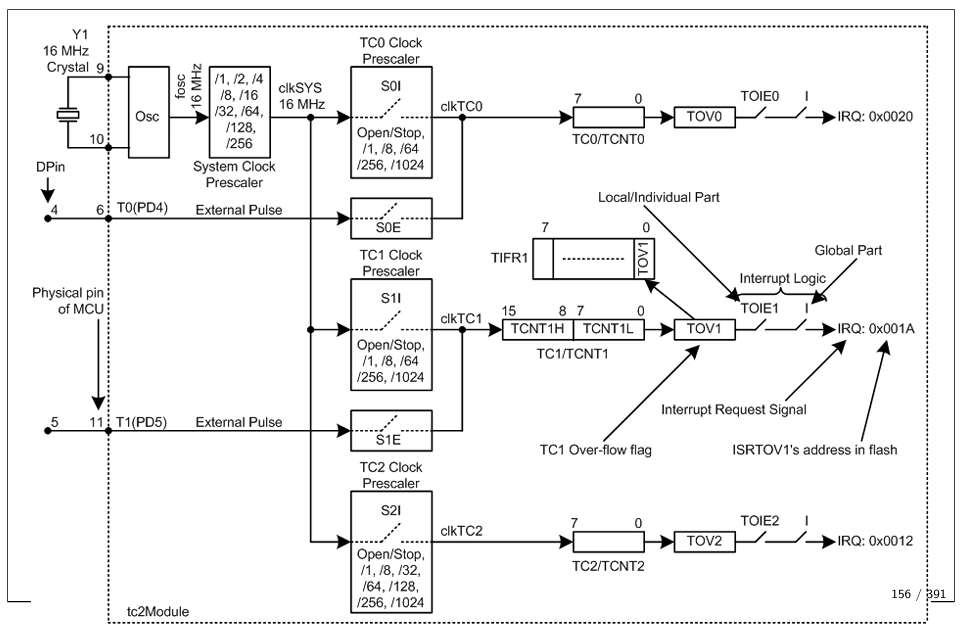
\includegraphics[width=0.75\textwidth]{Obrazky/Obrazky_DE2/fig_timer_structure.png}
    \caption{Štruktúra časovača ATmega328P. Hodinový signál (16 MHz) najprv prechádza predsdeličkou (prescaler), ktorá ho spomalí. Výsledný signál taktuje čítač TCNTn. Komparátor porovnáva TCNTn s hodnotou v OCRn. Výstupná jednotka autonómne generuje PWM na pine OCn.}
    \label{fig:timer_structure}
\end{figure}

\textbf{Preddelička (Prescaler):} hodinový signál 16 MHz je príliš rýchly pre väčšinu aplikácií. Preddelička ho vydelí pevnou hodnotou ($N \in \{1, 8, 64, 256, 1024\}$) a tým spomalí čítanie. S prescalerom 1024 sa čítač inkrementuje len $16\,000\,000 / 1024 \approx 15\,625\times$ za sekundu.

\section{Pretečenie -- čo sa stane, keď čítač dočíta}

8-bitový čítač počíta 0, 1, 2, \ldots, 254, 255 a potom \textbf{pretečie} späť na 0. Toto pretečenie (overflow) je dôležitá udalosť:
\begin{itemize}
    \item Nastaví sa príznak \textbf{TOVn} (Timer Overflow Flag)
    \item Ak je povolené prerušenie, CPU zavolá obslužnú rutinu
\end{itemize}

\begin{figure}[H]
    \centering
    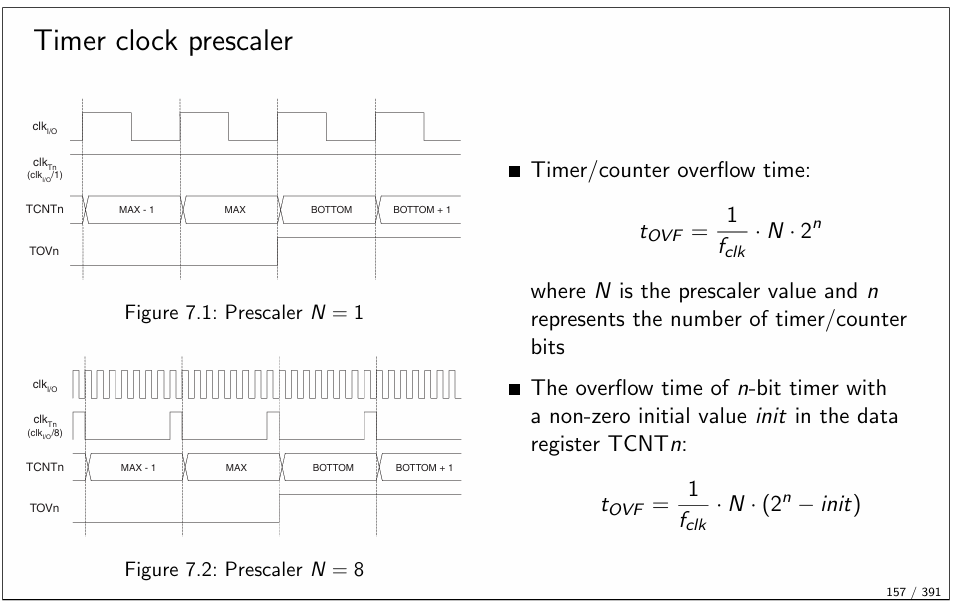
\includegraphics[width=0.80\textwidth]{Obrazky/Obrazky_DE2/fig_timer_overflow.png}
    \caption{Pretečenie čítača pri dvoch rôznych hodnotách prescaleru. Hore ($N=1$): čítač sa inkrementuje každý hodinový takt a preteká rýchlo. Dole ($N=8$): čítač sa inkrementuje len každý 8. takt -- preteká 8× pomalšie. Príznak TOVn sa nastaví vždy pri pretečení.}
    \label{fig:timer_overflow}
\end{figure}

\textbf{Ako vypočítať dobu pretečenia?} Čas pretečenia = (počet krokov čítača) × (perióda jedného kroku) = $2^n \times \dfrac{N}{f_{clk}}$.

Pre ATmega (16 MHz), Timer0 (8-bit), prescaler 64: $256 \times \dfrac{64}{16\,000\,000} = 1\,\text{ms}$ približne. Každú milisekundu pretečie.

\textbf{Inicializácia TCNTn:} ak nechceme čakať na plné pretečenie, načítame do TCNTn nenulovú hodnotu -- čítač potom začne od nej a pretečie skôr. Napr. načítame 206: čítač počíta 206, 207, \ldots, 255, potom pretečie. To je len 50 krokov namiesto 256.

\section{Komparácia -- presné časové intervaly}

Namiesto čakania na pretečenie môžeme nastaviť \textbf{porovnávaciu hodnotu v registri OCRn}. Komparátor neustále porovnáva TCNTn s OCRn. Pri zhode nastane \textbf{Compare Match}:
\begin{itemize}
    \item Nastaví sa príznak OCFn
    \item Môže sa vyvolať prerušenie
    \item Môže sa automaticky prepnúť výstupný pin (OCn)
\end{itemize}

\begin{figure}[H]
    \centering
    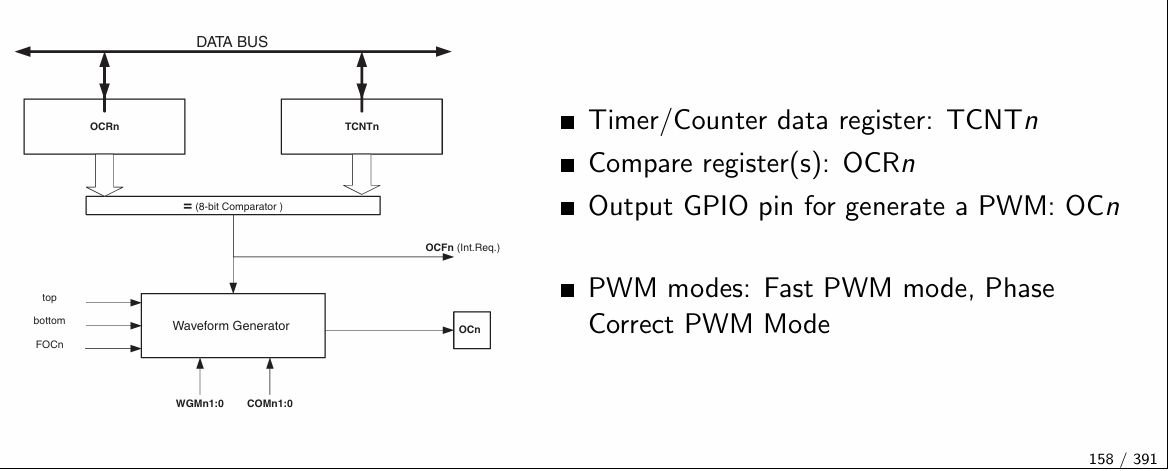
\includegraphics[width=0.65\textwidth]{Obrazky/Obrazky_DE2/fig_timer_compare.png}
    \caption{Blokové schéma komparačnej jednotky. Komparátor porovnáva TCNTn s OCRn. Pri zhode signalizuje zhodu (OCFn = prerušenie) a odovzdá pokyn Waveform Generatoru, ktorý podľa nastaveného módu (Fast PWM, Phase Correct PWM alebo CTC) riadi výstupný pin OCn.}
    \label{fig:timer_compare}
\end{figure}

\textbf{CTC mód (Clear Timer on Compare Match):} pri zhode TCNTn = OCRnA sa čítač \textbf{automaticky vynuluje} a začne znova od 0. Výsledkom je presne periodické prerušenie s nastaviteľnou periódou.

Praktické využitie: funkcia \texttt{millis()} v Arduine. Timer1 je nastavený v CTC móde tak, aby generoval prerušenie každú milisekundu. V obsluhe prerušenia sa inkrementuje globálna premenná -- a \texttt{millis()} ju len vráti.

\section{PWM -- riadenie výkonu digitálnym signálom}

\textbf{PWM (Pulse Width Modulation)} rieši problém: ako riadiť analógovú veličinu (jas LED, rýchlosť motora) digitálnym signálom (len 0 alebo 1)?

Riešenie: \textbf{signál rýchlo prepína medzi 0 a 1}. Ak je po väčšiu časť času v stave 1, priemerné napätie je vysoké -- LED svieti jasne. Ak je po väčšiu časť času v stave 0, priemerné napätie je nízke -- LED svieti slabo. Oko ani motor to nedokážu rozlíšiť.

\textbf{Strida (Duty Cycle):} pomer doby zapnutia k celkovej perióde, v percentách. 25\% strida = štvrtina periódy zapnutá. $V_{avg} = DC \cdot V_{CC}$.

\subsection{Fast PWM mód}

Čítač počíta \textbf{jedným smerom} -- od 0 nahor až do MAX, potom skočí späť na 0.

\begin{figure}[H]
    \centering
    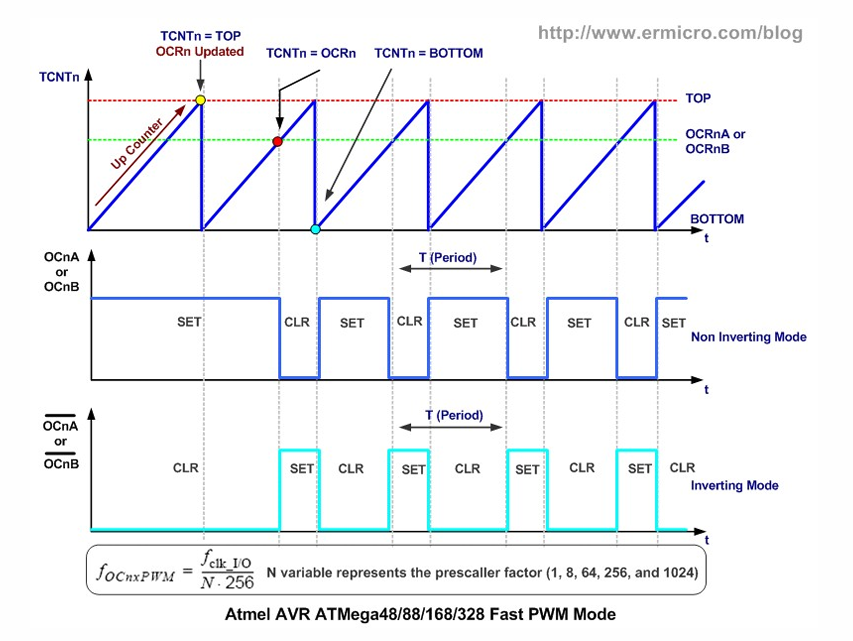
\includegraphics[width=0.75\textwidth]{Obrazky/Obrazky_DE2/fig_fast_pwm.png}
    \caption{Fast PWM mód. TCNTn (tučná píla) rastie od 0 do MAX, potom skočí späť. Výstup OCn sa nastaví na 1 vždy pri pretečení (TCNTn = 0) a vynuluje sa pri zhode s OCRn. Čím vyššie OCRn, tým dlhšia je časť s vysokou úrovňou -- tým vyššia strida. Frekvencia PWM závisí od hodinového kmitočtu, prescaleru a rozlíšenia čítača.}
    \label{fig:fast_pwm}
\end{figure}

Strida sa riadi hodnotou OCRn: OCRn = 0 znamená 0\% (stále nízka), OCRn = MAX znamená 100\% (stále vysoká). Frekvencia PWM je daná rýchlosťou čítania.

\subsection{Phase Correct PWM mód}

Čítač počíta \textbf{oboma smermi} -- nahor od 0 do MAX, potom nadol späť na 0.

\begin{figure}[H]
    \centering
    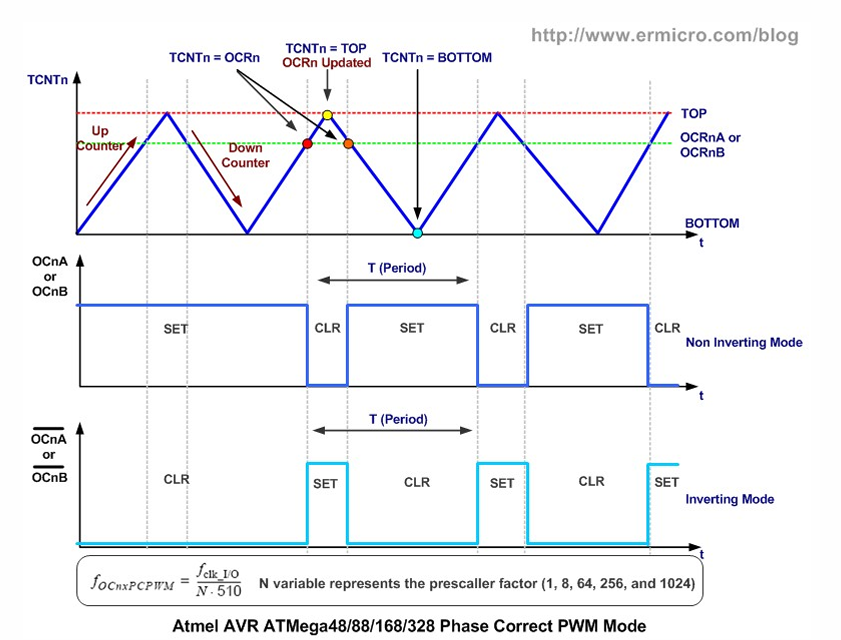
\includegraphics[width=0.75\textwidth]{Obrazky/Obrazky_DE2/fig_phase_correct_pwm.png}
    \caption{Phase Correct PWM mód. TCNTn tvorí trojuholníkový priebeh -- rastie a klesá. Výstup sa nuluje pri zhode na ceste nahor a nastavuje pri zhode na ceste nadol. Výsledný PWM pulz je symetrický okolo stredu periódy -- to je výhodné pre riadenie motorov.}
    \label{fig:phase_correct_pwm}
\end{figure}

\textbf{Prečo Phase Correct PWM pre motory?} Symetrický pulz spôsobuje menšie elektromagnetické rušenie. Navyše je fáza PWM na oboch kanáloch toho istého časovača vždy rovnaká -- to je dôležité pre H-mosty (riadenie smeru a rýchlosti motora).

\begin{center}
\begin{tabular}{lll}
\toprule
\textbf{Vlastnosť} & \textbf{Fast PWM} & \textbf{Phase Correct PWM} \\
\midrule
Smer čítania    & Jednosmerný (nahor)   & Obojsmerný (nahor/nadol) \\
Frekvencia      & Vyššia                & Približne polovičná \\
Symetria pulzu  & Nesymetrický          & Symetrický \\
Rušivosť (EMI)  & Vyššia                & Nižšia \\
Použitie        & LED, stmievanie, DAC  & Motory, servá \\
\bottomrule
\end{tabular}
\end{center}

%%%%%%%%%%%%%%%%%%%%%%%%%%%%%%%%%%%%%%%%%%%%%%%%%%%
\chapter{Sériová komunikácia UART a I2C}
%%%%%%%%%%%%%%%%%%%%%%%%%%%%%%%%%%%%%%%%%%%%%%%%%%%

\section{Prečo sériová komunikácia?}

Mikrokontroléry potrebujú komunikovať so senzormi, displejmi, GPS modulmi, Bluetooth, inými mikrokontrolérmi. Paralelná zbernica (8 vodičov pre 8 bitov) by bola drahá a nepraktická. \textbf{Sériová komunikácia} posiela bity jeden po druhom po jednom alebo dvoch vodičoch.

Kľúčové otázky každej sériovej komunikácie:
\begin{itemize}
    \item \textbf{Ako pozná prijímač, kde začína a končí jedno číslo (bajt)?} -- rámcovanie
    \item \textbf{Ako sa synchronizujú rýchlosti vysielača a prijímača?} -- synchronizácia
    \item \textbf{Ako sa na jednej zbernici rozlišujú rôzne zariadenia?} -- adresovanie
\end{itemize}

\section{UART -- najjednoduchšia sériová komunikácia}

UART (Universal Asynchronous Receiver/Transmitter) je najstarší a najjednoduchší sériový protokol. Prepája \textbf{presne dve zariadenia} dvoma vodičmi: TX (vysielanie) a RX (príjem).

\textbf{Asynchrónny} znamená: \textbf{žiadny zdieľaný hodinový signál}. Obe strany si musia dohodnúť rýchlosť (baud rate) vopred a každá si tiká vlastnými hodinami.

\subsection{Ako vyzerá UART rámec}

\begin{figure}[H]
    \centering
    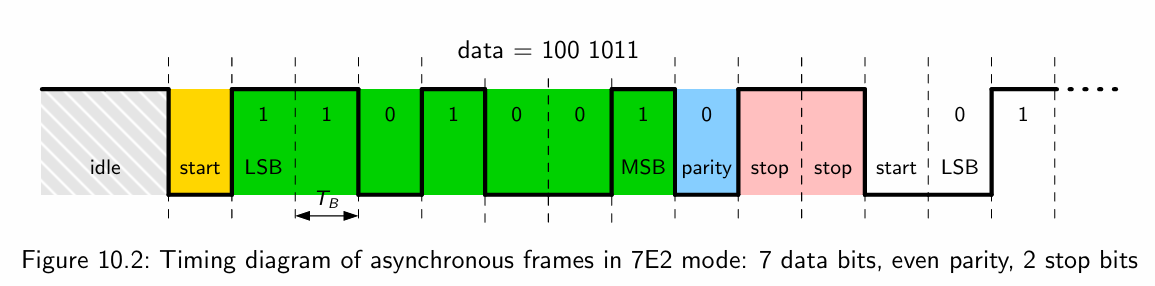
\includegraphics[width=0.85\textwidth]{Obrazky/Obrazky_DE2/fig_uart_frame.png}
    \caption{Časový diagram UART rámca (konfigurácia 7E2 pre prenos znaku 'K'). Linka je normálne v stave log. 1 (idle). Start bit (log. 0) upozorní prijímač. Potom prídu dátové bity od LSB. Paritný bit slúži na detekciu chýb. Jeden alebo dva stop bity (log. 1) ukončia rámec.}
    \label{fig:uart_frame}
\end{figure}

Každý bajt sa pošle ako \textbf{rámec}:
\begin{enumerate}
    \item \textbf{Start bit} (vždy log. 0): upozorní prijímač, že prichádzajú dáta
    \item \textbf{Dátové bity} (5--9, typicky 8): vlastné dáta, od LSB po MSB
    \item \textbf{Paritný bit} (voliteľný): súčet jednotiek, na detekciu jednoduchej chyby
    \item \textbf{Stop bit(y)}: linka sa vráti na log. 1, prijímač vie, že rámec skončil
\end{enumerate}

Označenie konfigurácie: \textbf{8N1} (8 dátových, bez parity, 1 stop -- najčastejší), \textbf{7E2} (7 dát, párna parita, 2 stop).

\textbf{Ako sa prijímač synchronizuje bez hodín?} Detekuje zostupnú hranu start bitu a potom vzorkuje každý bit v strede jeho časového okna. Interné hodiny prijímača tikajú 16× rýchlejšie ako baud rate -- start bit sa vzorkuje po 8 taktoch (stred), každý nasledujúci bit po 16 taktoch.

\textbf{Typické baud rates:} 9600, 19200, 57600, 115200 Bd (bitov za sekundu). Musia byť zhodné na oboch stranách!

\textbf{Využitie kanála:} pri 8N1 je z 10 prenesených bitov 8 dátových -- \textbf{80\% efektívnosť}. Zvyšných 20\% sú start a stop bity (réžia).

\textbf{Chybové príznaky:}
\begin{itemize}
    \item \textbf{Framing Error:} stop bit nie je log. 1 -- zlá rýchlosť alebo rušenie
    \item \textbf{Parity Error:} parita nesedí -- prevrátený jeden bit
    \item \textbf{Overrun Error:} nové dáta prišli skôr, ako CPU čítalo predchádzajúce
\end{itemize}

\subsection{USART v ATmega328P}

ATmega328P má perifériu USART na pinoch PD0 (RxD) a PD1 (TxD). Baud rate sa nastavuje zápisom do registra UBRR -- ten hovorí, koľkými hodinovými taktmi trvá jeden bit.

\section{I2C -- zbernica pre viac zariadení}

I2C (Inter-Integrated Circuit, vyslovuje sa ``I squared C'') vyvinul Philips v roku 1982 na prepojenie obvodov na jednej doske. Oproti UART pridáva kľúčové schopnosti: \textbf{viac zariadení na dvoch vodičoch} a \textbf{adresovanie}.

Iba \textbf{dva vodiče}:
\begin{itemize}
    \item \textbf{SCL} (Serial Clock): hodinový signál -- generuje ho vždy Master
    \item \textbf{SDA} (Serial Data): obojsmerná dátová linka
\end{itemize}

Oba vodiče sú cez odpory pripojené k napájaniu (pull-up). Každé zariadenie môže linku len \textbf{stiahnuť nadol} (open-drain) -- nikto linku aktívne nedvíha. Tým sa zabráni skratu pri kolízii.

Typické rýchlosti: 100 kHz (standard), 400 kHz (fast), 1 MHz (fast-plus).

\subsection{Ako I2C komunikácia prebieha -- krok za krokom}

\begin{figure}[H]
    \centering
    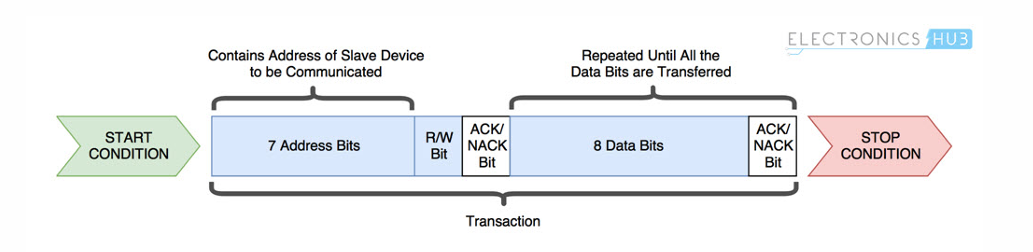
\includegraphics[width=0.85\textwidth]{Obrazky/Obrazky_DE2/fig_i2c_frame.png}
    \caption{Časový diagram I2C komunikácie. Dáta na SDA sú platné, keď SCL je vysoká. Start podmienka: SDA klesne, zatiaľ čo SCL je vysoká. Po Start podmienke Master pošle adresu Slave + bit R/W. Slave odpovie bitom ACK (stiahne SDA na 0). Potom sa prenášajú dátové bajty, každý potvrdený ACK. Stop podmienka: SDA stúpne pri vysokom SCL.}
    \label{fig:i2c_frame}
\end{figure}

\textbf{Celá sekvencia čítania z I2C senzora:}
\begin{enumerate}
    \item Master generuje \textbf{Start podmienku}: SDA klesne pri vysokom SCL -- všetky zariadenia to zaznamenajú
    \item Master pošle \textbf{7-bitovú adresu} Slave + bit R/W (0 = zápis)
    \item Oslovený Slave odpovie \textbf{ACK} (stiahne SDA na 0 v 9. takte) -- ostatné Slave ignorujú
    \item Master pošle \textbf{adresu registra}, z ktorého chce čítať; Slave potvrdí ACK
    \item Master generuje \textbf{Repeated Start} (nový Start bez Stop) + adresu Slave + bit R/W = 1 (čítanie)
    \item Slave pošle dáta; Master potvrdí ACK po každom bajte
    \item Po poslednom bajte Master pošle \textbf{NACK} (nestiahne SDA) -- signál, že nechce viac dát
    \item Master generuje \textbf{Stop podmienku}: SDA stúpne pri vysokom SCL
\end{enumerate}

\textbf{Clock Stretching:} Slave môže zdržať komunikáciu tým, že drží SCL nízko -- dáva si čas na spracovanie (napr. čaká na dokončenie merania). Master počká, kým Slave SCL neuvoľní.

\textbf{Repeated Start:} namiesto Stop + Start možno použiť Repeated Start (len nový Start bez Stop). Master tak udrží kontrolu nad zbernicou a prepne zo zápisu na čítanie v jednej transakcii.

\subsection{Adresovanie -- viac zariadení na jednej zbernici}

Každé I2C zariadenie má \textbf{unikátnu 7-bitovú adresu} (0--127, ale 16 je rezervovaných -- max. 112 zariadení). Adresa je buď pevne daná výrobcom, alebo čiastočne konfigurovateľná pomocou pinov (typicky 2--3 bity). Napríklad čip PCF8574 má základnú adresu 0x20 a piny A0--A2 umožňujú až 8 rôznych adries.

\subsection{I2C v ATmega328P -- TWI}

ATmega328P implementuje I2C ako \textbf{TWI (Two Wire Interface)} na pinoch PC4 (SDA) a PC5 (SCL). Frekvencia SCL sa nastavuje zápisom do registra TWBR.

\textbf{Príklady I2C zariadení:}
\begin{itemize}
    \item \textbf{DHT12}: senzor teploty a vlhkosti, adresa 0x5C
    \item \textbf{DS3231}: RTC hodiny reálneho času, adresa 0x68
    \item \textbf{AT24C32}: EEPROM pamäť 32 kB, adresa 0x57
    \item \textbf{PCF8574}: I/O expandér (pridá 8 GPIO pinov), adresy 0x20--0x27
\end{itemize}

\section{UART vs. I2C -- kedy čo použiť?}

\begin{center}
\begin{tabular}{lll}
\toprule
\textbf{Vlastnosť}    & \textbf{UART}                     & \textbf{I2C} \\
\midrule
Počet vodičov         & 2 (TX, RX)                        & 2 (SCL, SDA) \\
Počet zariadení       & 2 (point-to-point)                & Až 112 na jednej zbernici \\
Synchronizácia        & Asynchrónna (baud rate)           & Synchrónna (zdieľané hodiny) \\
Adresovanie           & Nie je -- priame spojenie         & 7-bitová adresa každého zariadenia \\
Duplex                & Full-duplex (súčasne oba smery)   & Half-duplex (striedavo) \\
Rýchlosť              & Až 115200 Bd (štd.)               & Až 400 kHz (fast mode) \\
Protokol              & Jednoduchý (len rámce)            & Zložitejší (Start/Stop/ACK) \\
Typické použitie      & Ladenie, GPS, Bluetooth, modem    & Senzory, EEPROM, RTC, displeje \\
\bottomrule
\end{tabular}
\end{center}

\textbf{UART volíme}, ak prepájame dve zariadenia, potrebujeme full-duplex alebo pracujeme s modulom, ktorý UART podporuje (GPS, Bluetooth modul, PC).

\textbf{I2C volíme}, ak pripájame viac senzorov alebo periférií k jednému mikrokontroléru a chceme šetriť piny (stačia vždy len 2 vodiče bez ohľadu na počet zariadení).
	% !TeX root = statnicaEKT.tex
\part{BPC-KS1 - Komunikační Systémy 1}
\begin{huge}
	Otázky:
	\newline
\end{huge}
\begin{enumerate}
	\item Otázka - Zdrojové a kanálové kódování (komprese hlasu, zvuku, videa a dat, konvoluční a blokové kódy).
	\item Otázka - Analogové a digitální pásmové modulace (amplitudové, fázové, kmitočtové, QAM). 
	\item Otázka - Synchronizace. Obvody pro obnovu nosné vlny a časování symbolů, metody rámcové a síťové synchronizace. 
\end{enumerate}

%%%%%%%%%%%%%%%%%%%%%%%%%%%%%%%%%%%%%%%%%%%%%%%%%%%
\chapter{Zdrojové a kanálové kódovanie}
%%%%%%%%%%%%%%%%%%%%%%%%%%%%%%%%%%%%%%%%%%%%%%%%%%%

\section{Zdrojové kódovanie -- kompresia signálov}

Cieľom zdrojového kódovania je odstrániť z prenášaného signálu nadbytočné
informácie a znížiť tak potrebný dátový tok. Prezentácia rozlišuje dva pojmy:

\begin{itemize}
    \item \textbf{Redundancia} -- množstvo znakov alebo bitov, ktoré možno eliminovať bez
        straty užitočnej informácie. Jej odstránením vzniká \textit{bezstratová kompresia}.
        Príklady: ZIP, PNG, Huffmanov kód, LZW (Lempel--Ziv--Welch).
    \item \textbf{Irelevancia} -- nepodstatná zložka informácie, ktorú možno potlačiť pri
        zachovaní požadovanej kvality signálu. Jej odstránením vzniká \textit{stratová kompresia}.
        Príklady: MP3, JPEG (Joint Photographic Experts Group), MPEG (Moving Picture Experts Group).
\end{itemize}

\subsection{Kódovanie rečových signálov}

\subsubsection{PCM -- pulzná kódová modulácia (Pulse Code Modulation)}

PCM je základný spôsob prevodu analógového signálu do digitálnej podoby -- ide
o analógovo-digitálny (A/D) prevodník. Princíp pozostáva z troch krokov:

\begin{enumerate}
    \item \textbf{Vzorkovanie} -- signál sa meria v pravidelných intervaloch (pre hlas
        typicky 8\,000-krát za sekundu). Musí byť splnený Nyquistov--Shannonov
        teorém: vzorkovací kmitočet $f_s \geq 2f_m$, kde $f_m$ je najvyšší kmitočet
        v spektre signálu. Pri nesplnení dochádza k aliasingu -- prekryvu spektrálnych
        zložiek.
    \item \textbf{Kvantovanie} -- každý vzorek sa zaokrúhli na najbližšiu kvantovaciu
        úroveň. Pre $N$ bitov existuje $M = 2^N$ úrovní. Chyba zaokrúhlenia tvorí
        kvantovací šum, ktorého efektívna hodnota je $N_{RMS} = \Delta U / \sqrt{12}$.
        Každý pridaný bit zlepší odstup signál/šum SNR (Signal to Noise Ratio) o $6\,\mathrm{dB}$.
    \item \textbf{Kódovanie} -- každej úrovni sa priradí binárne číslo (pri 8 bitoch
        existuje 256 úrovní, čo zodpovedá dátovému toku 64\,kbit/s pre telefónny hlas).
\end{enumerate}

\begin{figure}[H]
    \centering
    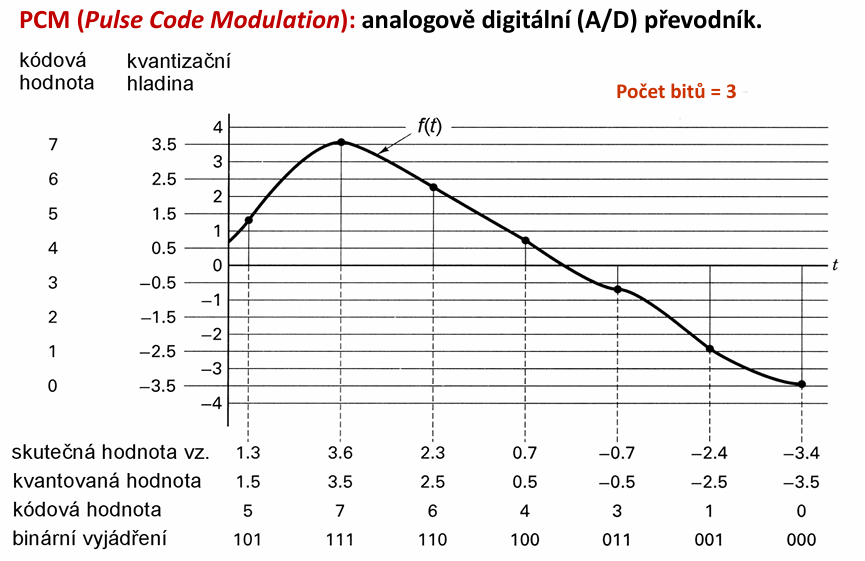
\includegraphics[width=0.85\textwidth]{Obrazky/Obrazky_KS1/fig_pcm_kvantovani.png}
    \caption{PCM -- lineárne kvantovanie. Vzorkovaný signál je priradený k najbližšej
    kvantovacej úrovni. Pre 3 bity existuje 8 úrovní. Kvantovací šum vzniká
    rozdielom skutočnej a kvantovanej hodnoty.}
    \label{fig:pcm}
\end{figure}

\textbf{Lineárne vs. nelineárne kvantovanie:} V ľudskej reči prevládajú nízke
hlasitosti -- veľké amplitúdy sú málo časté. Pri lineárnom kvantovaní by úseky s
malou amplitúdou boli kvantované s veľkou relatívnou chybou. Preto sa v praxi
(telefónia) používa \textbf{nelineárne kvantovanie} (A-law v Európe, $\mu$-law v
USA): pri malých amplitúdach sú kvantizačné kroky jemné (je ich viac), pri veľkých
hrubé (je ich menej). Výsledkom je rovnaká subjektívna kvalita pri menšom počte
bitov.

\subsubsection{DPCM -- diferenčná pulzná kódová modulácia (Differential Pulse Code Modulation)}

Susedné vzorky rečového signálu sú si veľmi podobné, pretože rečový signál je
časovo korelovaný. Namiesto absolútnej hodnoty vzorku sa preto prenáša \textbf{iba
rozdiel medzi skutočnou hodnotou a hodnotou predikovanou} z predchádzajúcich vzorkov.

\begin{figure}[H]
    \centering
    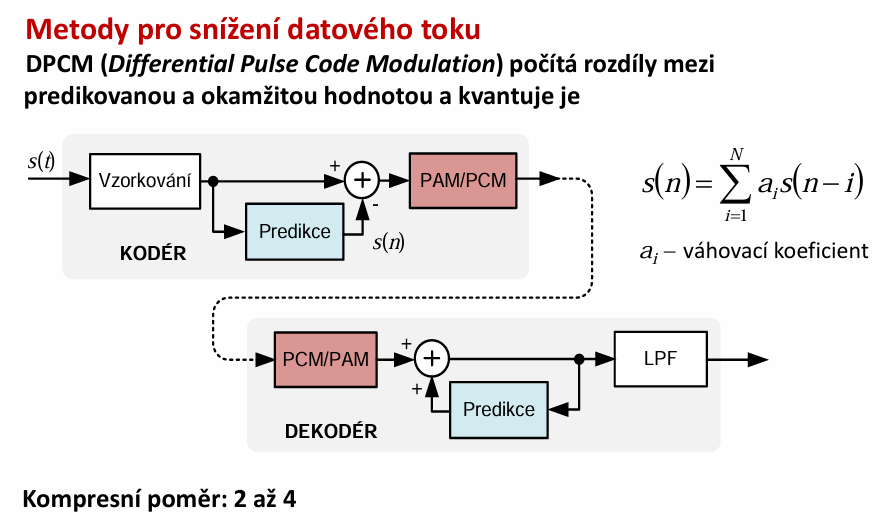
\includegraphics[width=0.80\textwidth]{Obrazky/Obrazky_KS1/fig_dpcm.png}
    \caption{Blokové schéma DPCM kodéra (hore) a dekodéra (dole). Kodér vypočíta
    rozdiel medzi skutočnou a predikovanou hodnotou vzorku a tento (malý) rozdiel
    prenáša. Dekodér pripočíta prijatý rozdiel k vlastnej predikcii a rekonštruuje
    signál.}
    \label{fig:dpcm}
\end{figure}

Prenáša sa iba predikčná chyba, ktorá má typicky malý rozptyl -- na jej zakódovanie
stačí menej bitov. Dosiahnuteľný \textbf{kompresný pomer je 2 až 4} oproti PCM.

\subsubsection{Vokodér -- parametrické kódovanie hlasu}

Vokodér nevysiela tvar zvukového signálu, ale \textbf{parametre modelu ľudského
hlasového traktu}. Vychádza z anatómie: znelé hlásky vznikajú periodickými impulzmi
hlasiviek (glottis), neznelé hlásky šumovým signálom z úst -- oba budiace signály
prechádzajú cez hlasový trakt (krk, ústa, nos), ktorý funguje ako filter.

\begin{figure}[H]
    \centering
    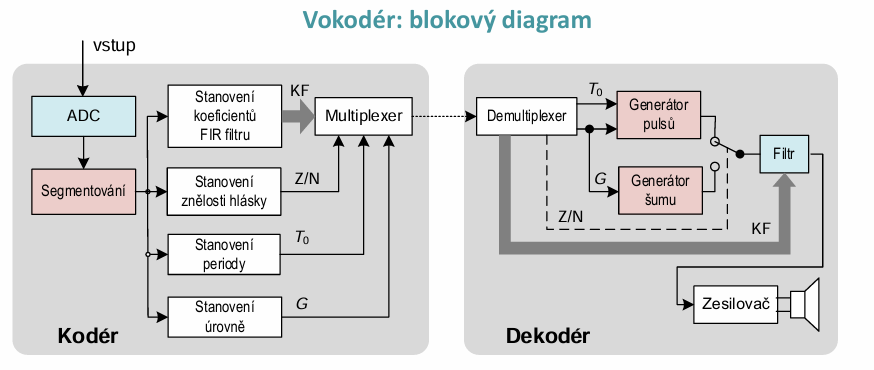
\includegraphics[width=0.85\textwidth]{Obrazky/Obrazky_KS1/fig_vokoder.png}
    \caption{Blokové schéma vokodéra. Kodér analyzuje reč po krátkych úsekoch
    (10--30\,ms -- parametre hlasového traktu sú v tomto úseku konštantné) a
    určuje: koeficienty filtra (KF), znelosť/neznelosť hlásky (Z/N), periódu
    základného tónu ($T_0$) a hlasitosť ($G$). Tieto parametre sa prenášajú.
    Dekodér budením príslušného generátora cez syntetický filter rekonštruuje reč.}
    \label{fig:vokoder}
\end{figure}

Namiesto tisícov vzorkov signálu sa prenáša iba niekoľko parametrov každých
20\,ms. Kvalita syntetizovanej reči je nižšia, ale dátový tok môže byť veľmi malý
(pod 4\,kbit/s).

\textbf{CELP} (Code Excited Linear Prediction -- lineárna predikcia s kódovým
budením): moderná varianta -- budený signál sa vyberá z vopred uloženého slovníka
(codebook) excitačných vektorov. Prenáša sa iba adresa (index) najlepšieho vektora.
Dosahuje rýchlosť 4\,kbit/s a menej. Používa sa v mobilných sieťach GSM (Global
System for Mobile Communications) a 3G.

\subsubsection{MPEG -- kódovanie zvuku}

MP3 a ostatné formáty MPEG využívajú \textbf{psychoakustický model} -- vlastnosti
ľudského sluchu:

\begin{itemize}
    \item \textbf{Kmitočtové maskovanie}: silný tón na určitom kmitočte maskuje slabšie
        tóny vo svojom frekvenčnom okolí -- tie sa stávajú pre poslucháča nepočuteľnými.
        Kmitočtové maskovacie krivky určujú, ako dielčie čisté tóny maskujú zvuky
        v ich okolí.
    \item \textbf{Časové maskovanie}: silný zvuk saturuje receptory vo vnútornom uchu
        a je potrebná určitá doba pre obnovenie ich činnosti -- zvuky bezprostredne
        pred a po hlasnom zvuku sú ťažšie rozoznateľné.
    \item Zložky signálu pod prahom sluchu sú nevnímateľné a neprenášajú sa.
\end{itemize}

Postup kódovania MPEG: signál sa rozdelí bankou filtrov do 32 subpásiem, pomocou
psychoakustického modelu sa určia maskovacie úrovne v každom subpásme a každému
pásmu sa pridelí zodpovedajúci počet bitov. Výsledok: subjektívne kvalitný zvuk
pri dátovom toku 128--320\,kbit/s namiesto 1\,411\,kbit/s pri CD.

\subsection{Kódovanie obrazu a videa}

\begin{itemize}
    \item \textbf{JPEG} (Joint Photographic Experts Group) -- transformačné kódovanie
        pre statické obrazy. Každý snímok sa rozdelí na bloky 8$\times$8 pixelov.
        Každý blok sa transformuje diskrétnou kosínusovou transformáciou DCT
        (Discrete Cosine Transform) do frekvenčnej oblasti a koeficienty zodpovedajúce
        vyšším priestorovým frekvenciám, ktoré sú pre ľudské oko menej dôležité,
        sa kvantujú hrubo alebo zahodia. Stratová kompresia fotografií.
    \item \textbf{MPEG} (Moving Picture Experts Group) -- hybridné kódovanie (DCT +
        prediktívne + vektory pohybu) pre pohyblivé obrazy. Navyše využíva
        \textit{časovú redundanciu}: po sebe idúce snímky videa sú si podobné.
        Prenášajú sa iba \textit{rozdiely} medzi snímkami a \textit{vektory pohybu}
        popisujúce posun objektov. Základ filmov, DVB (Digital Video Broadcasting),
        Blu-ray.
\end{itemize}

\subsection{Bezstratová kompresia dát}

\begin{itemize}
    \item \textbf{Huffmanov kód} -- neadaptívne kódovanie s preddefinovaným slovníkom.
        Symboly s vyššou pravdepodobnosťou výskytu dostávajú kratšie kódové slová,
        symboly s nižšou pravdepodobnosťou dlhšie. Priemerná dĺžka kódového slova
        sa tak minimalizuje.
    \item \textbf{LZW} (Lempel--Ziv--Welch) -- adaptívny slovníkový algoritmus
        s dynamicky vytváraným slovníkom. Hľadá opakujúce sa reťazce v dátach
        a nahrádza ich krátkymi kódmi. Používa sa v GIF, ZIP, ARJ.
\end{itemize}

%%%%%%%%%%%%%%%%%%%%%%%%%%%%%%%%%%%%%%%%%%%%%%%%%%%
\section{Kanálové kódovanie -- blokové a konvolucné kódy}
%%%%%%%%%%%%%%%%%%%%%%%%%%%%%%%%%%%%%%%%%%%%%%%%%%%

\section{Prečo kanálové kódovanie?}

Kanálové kódovanie zvyšuje odolnosť signálu proti chybám vznikajúcim pri prenose
komunikačným kanálom (vplyvom aditivného rušenia, medzisymbolových preslechov,
úniku signálu). Riešením je pridanie \textbf{zabezpečovacích (redundantných) bitov}
k prenášanej správe. Tieto bity umožnia prijímaču:
\begin{itemize}
    \item \textbf{Detegovať} chyby -- rozpoznať, že prijaté slovo nezodpovedá žiadnemu
        platnému kódovému slovu.
    \item \textbf{Opraviť} chyby bez nutnosti opakovania prenosu -- FEC (Forward Error
        Correction -- dopredná korekcia chýb).
\end{itemize}

Alternatívou je \textbf{ARQ} (Automatic Repeat reQuest -- automatická žiadosť
o opakovanie): detekcia chýb s požiadavkou na opakovanie chybného bloku. Vyžaduje
spätný kanál.

\textbf{Kódový pomer} $R = k/n$ udáva pomer počtu informačných bitov $k$ k
celkovému počtu bitov kódového slova $n$.

\subsection{Kľúčový pojem: Hammingova vzdialenosť}

\textbf{Hammingova vzdialenosť} $d(u, v)$ dvoch binárnych slov je počet pozícií,
v ktorých sa líšia. Napríklad pre $u = 10010$ a $v = 01011$ platí $d(u,v) = 3$.

\textbf{Minimálna Hammingova vzdialenosť} $d_{min}$ je najmenšia hodnota vzdialenosti
medzi všetkými kódovými slovami kódu. Určuje opravné schopnosti:
\begin{itemize}
    \item Maximálny zaručený počet detegovateľných chýb: $k_z = d_{min} - 1$
    \item Maximálny zaručený počet opraviteľných chýb: $k_o = \lfloor(d_{min}-1)/2\rfloor$
\end{itemize}

\subsection{Paritný kód -- najjednoduchší blokový kód}

K prenášanému slovu sa pridá jeden \textbf{paritný bit} tak, aby celkový počet
jednotiek bol párny (sudá parita). Prijímač skontroluje paritu -- ak je nepárna,
nastala chyba. Kód má $d_{min} = 2$, teda deteguje jednonásobné chyby, ale
nedokáže ich opraviť.

\textbf{Iteračný (súčinový) kód}: dáta sa usporiadajú do matice a paritné bity
sa počítajú pre každý riadok aj každý stĺpec. Umožňuje nielen detegovať, ale aj
\textbf{lokalizovať a opraviť} jednonásobnú chybu -- prienik chybného riadka a
chybného stĺpca jednoznačne určí pozíciu chybného bitu.

\subsection{Lineárne blokové kódy}

Lineárny blokový kód $(n, k)$ zobrazuje blok $k$ informačných bitov na kódové
slovo dĺžky $n$ bitov, pričom $n - k$ bitov tvorí zabezpečovaciu časť.

Kódovanie sa vykonáva pomocou \textbf{generujúcej matice} $\mathbf{G}$:
zabezpečovacie bity sú lineárnymi kombináciami (XOR -- eXclusive OR, exkluzívny
súčet) vybraných informačných bitov, každý kontroluje inú podmnožinu.

V prijímači sa vypočíta \textbf{syndróm} $\mathbf{s} = \mathbf{r} \cdot \mathbf{H}^T$,
kde $\mathbf{H}$ je kontrolná matica. Syndróm rovný nule indikuje bezchybný príjem;
nenulový syndróm jednoznačne určuje pozíciu chyby.

\subsection{Hammingove kódy}

Hammingove kódy sú lineárne kódy s $d_{min} = 3$, kde \textbf{binárna hodnota
syndrómu priamo udáva pozíciu chybného bitu} -- nie je potrebné žiadne vyhľadávanie
v tabuľke chýb.

Štruktúra kódu: k 4 informačným bitom sa pridajú 3 zabezpečovacie bity $\Rightarrow$
kód (7,4), $R = 4/7$. Zabezpečovacie bity sú umiestnené na pozíciách mocnín čísla
2 (1, 2, 4) a každý kontroluje iné podmnožiny bitov kódového slova.

\begin{figure}[H]
    \centering
    \includegraphics[width=0.65\textwidth]{Obrazky/Obrazky_KS1/fig_hamming_koder.png}
    \caption{Kodér Hammingovho kódu (7,4). Hradlá XOR počítajú kontrolné bity
    $c_1$, $c_2$, $c_4$ zo zdrojových bitov $m_3, m_5, m_6, m_7$. Výsledné
    kódové slovo: $[c_1\, c_2\, m_3\, c_4\, m_5\, m_6\, m_7]$.}
    \label{fig:hamming_koder}
\end{figure}

\begin{figure}[H]
    \centering
    \includegraphics[width=0.65\textwidth]{Obrazky/Obrazky_KS1/fig_hamming_dekoder.png}
    \caption{Dekodér Hammingovho kódu (7,4). Syndróm $[s_3\, s_2\, s_1]$ sa
    vypočíta z prijatého slova. Jeho binárna hodnota priamo zodpovedá pozícii
    chybného bitu (napr. syndróm $= 101_2 = 5 \Rightarrow$ chyba na 5. pozícii).
    Korekčná logika bit invertuje.}
    \label{fig:hamming_dekoder}
\end{figure}

Príklady: HK(7,4), HK(15,11), HK(31,26). Opravujú jednonásobné chyby ($t=1$).
Rozšírený Hammingov kód (pridanie globálneho paritného bitu) má $d_{min} = 4$:
opravuje jednonásobné a deteguje dvojnásobné chyby.

\subsection{Cyklické kódy}

Cyklické kódy sú špeciálne lineárne kódy s vlastnosťou: \textbf{cyklickým posunom
ľubovoľného kódového slova vznikne opäť platné kódové slovo}. Táto algebraická
štruktúra umožňuje implementovať kodéry a dekodéry pomocou jednoduchých posuvných
registrov so spätnou väzbou.

\textbf{CRC} (Cyclic Redundancy Check -- cyklická kontrola redundanciou) --
najpoužívanejší cyklický kód na detekciu chýb. Zabezpečovacie bity sa vypočítajú
ako zvyšok po delení polynomiálnou reprezentáciou dát generujúcim polynómom $g(x)$.
Prijímač overí, či je zvyšok nulový. Používa sa v Ethernete, USB (Universal Serial
Bus), ZIP, UART (Universal Asynchronous Receiver-Transmitter).

\textbf{BCH} (Bose--Chaudhuri--Hocquenghem) \textbf{a Reed-Solomonove kódy} --
pokročilejšie cyklické kódy schopné opravovať viac chýb ($t > 1$). Reed-Solomon
pracuje so symbolmi (skupinami bitov) a je obzvlášť účinný pri oprave
\textit{zhlukov chýb} -- používa sa v CD, DVD, QR kódoch a satelitnej komunikácii.

\subsection{Konvolucné kódy}

Konvolucné kodéry spracúvajú vstupnú postupnosť \textbf{kontinuálne} -- na rozdiel
od blokových kódov nepracujú s blokmi pevnej dĺžky. Každý výstupný bit je lineárnou
kombináciou (XOR) aktuálneho vstupného bitu a niekoľkých predchádzajúcich bitov
uchovaných v posuvnom registri (pamäť kodéra dĺžky $m$).

Parametre kódu: dĺžka bloku výstupného slova $n_0$, dĺžka bloku správy $k_0$,
kódový pomer $R = k_0/n_0$, dĺžka kódového obmedzenia $mk_0$.

\begin{figure}[H]
    \centering
    \includegraphics[width=0.50\textwidth]{Obrazky/Obrazky_KS1/fig_konvolucni_koder.png}
    \caption{Kodér konvolucného kódu s kódovým pomerom $R=1/2$ a dĺžkou pamäte
    $K=3$. Posuvný register uchováva aktuálny a dva predchádzajúce vstupné bity.
    Pre každý vstupný bit sa vygenerujú dva výstupné bity ako rôzne XOR kombinácie
    obsahu registra.}
    \label{fig:konv_koder}
\end{figure}

\textbf{Mriežkový (trellis) diagram} je grafická reprezentácia všetkých možných
stavových prechodov kodéra. Každý uzol reprezentuje stav posuvného registra,
každá hrana zodpovedá jednému vstupnému bitu a je označená zodpovedajúcimi
výstupnými bitmi. Pre vstupnú postupnosť dĺžky $L$ existuje na $L$-tej úrovni
stromu $2^L$ rozvetvení, ale iba $2^m$ rôznych stavov -- preto sa prechádza na
mriežkový diagram.

\begin{figure}[H]
    \centering
    \includegraphics[width=0.80\textwidth]{Obrazky/Obrazky_KS1/fig_trellis.png}
    \caption{Mriežkový (trellis) diagram konvolucného kodéra s $K=3$. Štyri uzly
    zodpovedajú stavom posuvného registra (00, 10, 01, 11). Horné vetvy = vstupný
    bit 0, dolné vetvy = vstupný bit 1. Kódovanie správy
    $\mathbf{m}=[1\,1\,0\,1\,1]$ = tučne vyznačená cesta diagramom.}
    \label{fig:trellis}
\end{figure}

\subsubsection{Viterbiho algoritmus -- dekódovanie konvolucných kódov}

Viterbiho dekódovanie je optimálne dekódovanie s maximálnou vierohodnosťou
(ML -- Maximum Likelihood decoding) -- porovnávanie prijatej, chybami narušenej
postupnosti so všetkými postupnosťami, ktoré mohli byť vyslané.

\textbf{Viterbiho algoritmus} využíva princíp dynamického programovania:
\begin{enumerate}
    \item V každom časovom kroku sa vypočíta Hammingova vzdialenosť prijatého
        bloku dĺžky $n_0$ od všetkých možných blokov na každej vetve diagramu.
    \item Kumulovaná metrika (súčet vzdialeností) každej cesty sa priebežne
        aktualizuje.
    \item V rámci okna konečnej dĺžky sa v každom uzle zachová iba
        \textbf{prežívajúca cesta} (survivor path) -- tá s najmenšou kumulovanou
        metrikou; ostatné cesty sa eliminujú.
    \item Na konci sa vyberie cesta s minimálnou celkovou metrikou -- tá
        zodpovedá dekódovanej správe.
\end{enumerate}

\begin{figure}[H]
    \centering
    \includegraphics[width=0.85\textwidth]{Obrazky/Obrazky_KS1/fig_viterbi.png}
    \caption{Viterbiho dekódovací algoritmus -- kroky a) až d). Čísla pri uzloch
    sú kumulované Hammingove vzdialenosti (metriky ciest). V každom kroku sa
    eliminujú cesty s vyššou metrikou (prerušované čiary). Nakoniec zostane
    jediná optimálna cesta.}
    \label{fig:viterbi}
\end{figure}

\textbf{Tvrdé vs. mäkké rozhodovanie:}
\begin{itemize}
    \item \textbf{Tvrdé rozhodovanie} (hard decision): demodulátor kvantuje každý
        prijatý symbol na 0 alebo 1. Metrikou vetvy je Hammingova vzdialenosť.
        Jednoduché, ale vedie k strate informácie o spoľahlivosti rozhodnutia.
    \item \textbf{Mäkké rozhodovanie} (soft decision): demodulátor odovzdá dekodéru
        nekvantované hodnoty. Metrikou vetvy je euklidovská vzdialenosť. Zlepšenie
        oproti tvrdému rozhodovaniu je približne 2--3\,dB.
\end{itemize}

\textbf{Turbokódy}: dva konvolucné kodéry zapojené paralelne s prekladačom
(interleaverom) medzi nimi. Iteračné turbo dekódovanie s výmenou extrinsických
informácií medzi dekodérmi dosahuje výkon veľmi blízky Shannonovmu limitu kapacity
kanála. Používajú sa v LTE (Long Term Evolution, 4G).

%%%%%%%%%%%%%%%%%%%%%%%%%%%%%%%%%%%%%%%%%%%%%%%%%%%
\chapter{Analógové a digitálne pásmové modulácie}
%%%%%%%%%%%%%%%%%%%%%%%%%%%%%%%%%%%%%%%%%%%%%%%%%%%

\section{Prečo modulácia?}

Signál základného pásma moduluje sínusový priebeh -- \textbf{nosnú vlnu} -- tak,
aby zodpovedal charakteristikám prenosového kanálu. Nosná sa prevádza na
elektromagnetické pole (EM pole) za účelom šírenia na požadované miesto určenia
pomocou antén.

Klasifikácia modulácií:
\begin{itemize}
    \item Analógové (AM, FM, PM, QAM) vs. digitálne (ASK, FSK, PSK, QAM)
    \item Lineárne (s premennou modulačnou obálkou): AM (Amplitude Modulation),
        QAM (Quadrature Amplitude Modulation), ASK (Amplitude Shift Keying)
    \item Nelineárne (s konštantnou modulačnou obálkou): FM (Frequency Modulation),
        PM (Phase Modulation), FSK (Frequency Shift Keying), PSK (Phase Shift Keying)
    \item Koherentné (demodulácia s pomocou obnovenej nosnej): ASK, FSK, PSK
    \item Nekoherentné (demodulácia bez obnovenej nosnej): DPSK (Differential PSK),
        FSK, ASK
\end{itemize}

Harmonický signál $s_0(t) = S_0\cos(2\pi f_c t + \varphi_0)$ má tri parametre,
ktoré možno modulovať: amplitúdu $S_0$ (AM, ASK), kmitočet $f_c$ (FM, FSK)
a fázu $\varphi_0$ (PM, PSK).

\section{Amplitúdové modulácie}

\subsection{AM -- amplitúdová modulácia (Amplitude Modulation)}

Typické aplikácie: rozhlasové vysielanie na dlhých LW (Long Wave), stredných MW
(Medium Wave) a krátkych SW (Short Wave) vlnách (kmitočty od stoviek kHz do
jednotiek MHz) pri výkonoch v stovkách kW.

Amplitúda nosnej je lineárnou funkciou modulačného signálu. Obálka AM signálu:
$S(t) = S_0 + \Delta S \cdot n(t)$, kde $m = \Delta S / S_0$ je \textbf{hĺbka
modulácie} (typicky sa udáva v percentách, $0 < m \leq 1$) a $n(t)$ je normovaná
modulačná funkcia.

Spektrum AM signálu obsahuje tri zložky: nosnú na $f_c$ a dve postranné pásma
na $f_c \pm F$ (kde $F$ je kmitočet modulačného signálu).

\textbf{Výhoda AM}: jednoduchá asynchrónna demodulácia obálkovým demodulátorem
(dióda + RC článok) -- nevyžaduje obnovu nosnej.

\textbf{Hlavná nevýhoda AM}: je energeticky neefektívna. Vysielač musí byť
dimenzovaný na špičkový výkon $P_{PEP} = 4P_0$ (pri $m = 1$), pritom modulačná
účinnosť je len $\eta = 33\,\%$ -- nosná nenesie informáciu, ale spotrebuje
väčšinu výkonu.

\begin{figure}[H]
    \centering
    \includegraphics[width=0.88\textwidth]{Obrazky/Obrazky_KS1/fig_am_casova_oblast.png}
    \caption{AM signál v časovej oblasti. Hore: normovaný modulačný signál $n(t)$.
    Dole: AM signál $s(t)$ s obálkou $S(t)$. Bez modulácie má nosná konštantnú
    amplitúdu $S_0$; po zapnutí modulácie sa amplitúda mení od $A_{min} = S_0(1-m)$
    do $S_{max} = S_0(1+m)$ podľa modulačného signálu. Amplitudový zdvih je
    $\Delta S = mS_0$.}
    \label{fig:am_casova}
\end{figure}

\subsection{DSB -- obidve postranné pásma s potlačenou nosnou (Double Side Band -- Suppressed Carrier)}

Nosná zložka je potlačená -- \textbf{modulačná účinnosť je 100\,\%}, všetok
výkon je sústredený v postranných pásmach nesúcich informáciu. Demodulácia
vyžaduje koherentnú referenciu -- obnovu nosnej vlny v prijímači (umocňujúca
slučka, Costasova slučka).

\subsection{SSB -- jedno postranné pásmo (Single Side Band)}

Obidve postranné pásma DSB obsahujú tú istú informáciu -- prenáša sa iba jedno z
nich. SSB má \textbf{polovičnú šírku pásma} oproti DSB.

Výhody: maximálna spektrálna efektívnosť, väčší dosah pri rovnakom výkone.
Nevýhody: zložitejší modulátor (fázová metóda alebo filtrová metóda) a nutnosť
koherentnej demodulácie. Používa sa na krátkych vlnách (rádioamatéri, letecká
komunikácia).

\subsection{VSB -- vestigiálne postranné pásmo (Vestigial Side Band)}

Kompromis medzi DSB a SSB. Jedno postranné pásmo sa prenesie celé, z druhého
sa prenesie iba vestigium (zvyšok) v okolí nosnej. Realizuje sa nesymetrickým
pásmovým filtrom. Používa sa pri prenose obrazového signálu v analógovom
televíznom vysielaní.

\subsection{QAM -- kvadratúrna amplitúdová modulácia (Quadrature Amplitude Modulation)}

QAM používa dve nosné vlny v kvadratúre ($\sin\omega_c t$ a $\cos\omega_c t$).
Sú navzájom ortogonálne -- vzájomne sa neovplyvňujú -- a QAM tak môže prenášať
\textbf{dva nezávislé modulačné signály} $n_1$ a $n_2$ rovnakým kanálom (lepšie
využitie kanála). Je základom digitálnych M-stavových modulácií QAM a používa
sa v televíznom systéme PAL (Phase Alternating Line) pre prenos chrominančných
zložiek.

\section{Uhlové modulácie (FM a PM)}

Pri uhlových moduláciách zostáva amplitúda nosnej konštantná $S(t) = S_0$ --
informácia je zakódovaná v okamžitej fáze nosnej.

\textbf{Výhoda}: konštantná obálka signálu umožňuje použiť nelineárne zosilňovače
triedy C s vyššou energetickou účinnosťou. Amplitúdové rušenie (atmosferické
poruchy, viacestné šírenie) nemá vplyv -- prijímač ho potlačí amplitúdovým
obmedzovačom.

\subsection{FM -- kmitočtová modulácia (Frequency Modulation)}

Okamžitý kmitočet nosnej je lineárnou funkciou modulačného signálu:
$f_i(t) = f_0 + \Delta f \cdot n(t)$, kde $\Delta f$ je \textbf{kmitočtový zdvih}
a $n(t)$ je normovaná modulačná funkcia.

\textbf{Index modulácie} $\beta = \Delta f / F$ (pomer kmitočtového zdvihu
k najvyššiemu kmitočtu modulačného signálu) rozlišuje:
\begin{itemize}
    \item $\beta \gg 1$: širokopásmová FM WBFM (Wideband FM) -- rozhlasové vysielanie
        CCIR (Consultative Committee for International Radio) 88,5--108\,MHz,
        $\Delta f = 75\,\mathrm{kHz}$
    \item $\beta \ll 1$: úzkopásmová FM NBFM (Narrowband FM) -- pozemné služby,
        pojítka, polícia, hasiči
\end{itemize}

\textbf{Šírka pásma FM} -- Carsonovo pravidlo: $B_A = 2F_{max}(\beta + 1) =
2(\Delta f + F_{max})$. Pre FM rozhlas: $B_A \approx 200\,\mathrm{kHz}$.

\textbf{Demodulácia FM}: kmitočtový diskriminátor, koincidenčný demodulátor,
alebo demodulátor so slučkou PLL (Phase-Locked Loop).

\begin{figure}[H]
    \centering
    \includegraphics[width=0.92\textwidth]{Obrazky/Obrazky_KS1/fig_fm_spektrum.png}
    \caption{Vľavo: reálne FM spektrum namerané spektrálnym analyzátorom
    ($f_c = 10\,\mathrm{MHz}$, $F = 10\,\mathrm{kHz}$, $\beta = 5$). Spektrálne
    čiary sú rozmiestnené po $F$ okolo nosnej $f_0$ a ich amplitúdy sú dané
    Besselovými funkciami $S_0 J_k(\beta)$. Vpravo: priebeh Besselových funkcií
    prvého druhu $J_k(\beta)$ pre rôzne rády $k$ -- určujú výkony jednotlivých
    spektrálnych zložiek FM signálu. Carsonovo pravidlo: $B_{FM} = 2(F + \Delta f)$
    zahŕňa 98\,\% výkonu signálu.}
    \label{fig:fm_spektrum}
\end{figure}

\subsection{PM -- fázová modulácia (Phase Modulation)}

Okamžitá fáza nosnej je lineárnou funkciou modulačného signálu. FM a PM sú si
vzájomne príbuzné: FM zo signálu PM sa získa zaradením integrátora pred PM
modulátor a naopak.

\section{Digitálne modulácie v prenesenom pásme}

Pri digitálnych moduláciách nosná nadobúda diskrétne stavy zodpovedajúce
prenášaným symbolom. Počet stavov $M = 2^n$ určuje počet bitov na symbol $n$.
Vyšší počet stavov zvyšuje spektrálnu efektívnosť [bit/s/Hz], ale znižuje odolnosť
voči šumu -- body konštelačného diagramu sú si bližšie.

\subsection{BPSK a QPSK -- fázové kľúčovanie}

\textbf{BPSK} (Binary Phase Shift Keying -- binárne fázové kľúčovanie): $M = 2$
fázové stavy (0° a 180°), 1 bit/symbol. Najvyššia odolnosť voči šumu spomedzi
PSK modulácií. Používa sa pri nízkych hodnotách $E_b/N_0$ (satelitné spoje, GPS --
Global Positioning System).

\textbf{QPSK} (Quadrature Phase Shift Keying -- kvadratúrne fázové kľúčovanie):
$M = 4$ fázové stavy, 2 bity/symbol. Pri rovnakej šírke pásma ako BPSK prenesie
dvojnásobok dát. Konštelačný diagram: 4 body v rohoch štvorca.

\textbf{$\pi/4$-DQPSK} (Differential Quadrature PSK -- diferenčné QPSK):
diferenčná varianta QPSK, kde sa prenáša zmena fázy oproti predchádzajúcemu
symbolu (nie absolútna fáza). Umožňuje nekoherentnú demoduláciu.
Používa sa v systéme GSM EDGE (Enhanced Data rates for GSM Evolution).

\textbf{8PSK} (8 Phase Shift Keying): $M = 8$ fázových stavov, 3 bity/symbol.
Dobrá spektrálna účinnosť (teoreticky 3\,bit/s/Hz). Problém s obnovením nosnej
(neistota $\pm\pi/8$). Používa sa v GSM EDGE.

\begin{figure}[H]
    \centering
    \includegraphics[width=0.82\textwidth]{Obrazky/Obrazky_KS1/fig_qpsk_konstelacia.png}
    \caption{Tabulka stavov I a Q a konštelačný (vektorový) diagram QPSK.
    Nosná nadobúda 4 fázové stavy $\pm 45°$ a $\pm 135°$. Každý stav zodpovedá
    jednému dibitu (dvojici bitov). QPSK je štvorstavová QAM s potlačenou
    nosnou -- generuje sa násobením dvoch ortogonálnych nosných ($\cos$ a $\sin$)
    dvoma NRZ (Non-Return-to-Zero) signálmi I a Q.}
    \label{fig:qpsk_konstelacia}
\end{figure}

\subsection{M-QAM -- kvadratúrna amplitúdová modulácia (Quadrature Amplitude Modulation)}

Informácia je zakódovaná súčasne v amplitúde aj fáze nosnej -- body konštelačného
diagramu tvoria pravouhlú mriežku. Pri vyššom $M$ sa zvyšuje spektrálna
efektívnosť, ale klesá odolnosť voči šumu.

\begin{itemize}
    \item 16-QAM: mriežka 4$\times$4, 4 bity/symbol -- DVB-T (Digital Video
        Broadcasting -- Terrestrial), Wi-Fi
    \item 64-QAM: mriežka 8$\times$8, 6 bitov/symbol -- káblová TV DVB-C
        (Digital Video Broadcasting -- Cable)
    \item 256-QAM: 8 bitov/symbol -- vyžaduje vysoký odstup signál/šum
\end{itemize}

\subsection{MSK a GMSK -- kmitočtové kľúčovanie so spojitou fázou}

\textbf{MSK} (Minimum Shift Keying -- kľúčovanie s minimálnym zdvihom) je členem
skupiny modulácií FSK so spojitou fázou CPFSK (Continuous Phase FSK). Pri zmene
signalizačných kmitočtov je zabezpečená plynulá zmena fázy -- bez fázových skokov.
Index modulácie $\beta = 0{,}5$ -- ide o minimálny zdvih, pri ktorom sú oba nosné
kmitočty ešte ortogonálne. Vlastnosti: možnosť nekoherentnej demodulácie, dobrá
výkonová a spektrálna účinnosť.

\textbf{GMSK} (Gaussian Minimum Shift Keying -- MSK s Gaussovým filtrom): pred
modulátor MSK je zaradená Gaussovská dolná priepusť GLPF (Gaussian Low Pass Filter).
Tá kmitočtovo obmedzí spektrum klíčovacieho signálu, čím sa výrazne potlačia
postranné laloky kmitočtového spektra modulovaného signálu. Výsledný signál GMSK
nemusí byť ďalej filtrovaný. Používa sa v GSM.

\begin{figure}[H]
    \centering
    \includegraphics[width=0.90\textwidth]{Obrazky/Obrazky_KS1/fig_msk_prubehy.png}
    \caption{MSK -- príklad modulácie. Vľavo hore: dátový signál $d(t)$;
    uprostred: fázová mriež $\Phi_{MSK}(t)$ -- fáza rastie alebo klesá lineárne
    o $\pm\pi/2$ počas každej bitovej periódy $T_b$, čo zabezpečuje plynulú spojitú
    fázu; dole: výsledný MSK signál $s_{MSK}(t)$ bez fázových skokov.
    Vpravo hore: kruhový konštelačný diagram MSK (konštantná obálka).
    Vpravo dole: porovnanie spektier MSK a QPSK -- MSK má užšie hlavné laloky
    a rýchlejší pokles postranných lalokov.}
    \label{fig:msk_prubehy}
\end{figure}

\begin{figure}[H]
    \centering
    \includegraphics[width=0.90\textwidth]{Obrazky/Obrazky_KS1/fig_gmsk_spektrum.png}
    \caption{GMSK -- porovnanie s MSK. Vľavo: časový priebeh dátového signálu
    $d(t)$, fázovej mriže $\Phi_{MSK}(t)$ a výsledného GMSK signálu $s_{GMSK}(t)$ --
    Gaussovský filter zaobli ostré hrany fázovej mriže. Vpravo: skutočné spektrá
    namerané spektrálnym analyzátorom pre MSK (čierna) a GMSK s parametrami
    $BT_b = 0{,}4$ (modrá) a $BT_b = 0{,}6$ (zelená) -- GMSK má výrazne
    potlačené postranné laloky, čo znižuje medzikanálové interferencie.}
    \label{fig:gmsk_spektrum}
\end{figure}

%%%%%%%%%%%%%%%%%%%%%%%%%%%%%%%%%%%%%%%%%%%%%%%%%%%
\chapter{Synchronizácia}
%%%%%%%%%%%%%%%%%%%%%%%%%%%%%%%%%%%%%%%%%%%%%%%%%%%

\section{Prečo synchronizácia?}

Synchronizácia je neoddeliteľnou súčasťou každého digitálneho komunikačného
systému. Prijímač potrebuje poznať:
\begin{enumerate}
    \item \textbf{Presný kmitočet a fázu nosnej vlny} -- pri koherentnej demodulácii
        musí lokálne generovaná referenčná nosná byť v kmitočtovej a fázovej zhode
        s nosnou prijatého signálu. Fázová odchýlka spôsobuje rotáciu konštelačného
        diagramu a zvyšuje chybovosť.
    \item \textbf{Optimálne okamihy vzorkovania demodulovaného signálu} $T_m$ --
        vzorkovanie v okamihu maximálneho otvorenia oka minimalizuje chybovosť.
        Vzorkovanie mimo optima znižuje odstup signál/šum.
    \item \textbf{Polohu hraníc dátových rámcov} -- pri blokovom prenose a kanálovom
        kódovaní je nutné poznať začiatok každého kódového slova alebo rámca.
\end{enumerate}

\section{Diagram oka -- hodnotenie kvality synchronizácie}

\begin{figure}[H]
    \centering
    \includegraphics[width=0.55\textwidth]{Obrazky/Obrazky_KS1/fig_oko.png}
    \caption{Diagram oka vznikne superpozíciou časových priebehov demodulovaného
    signálu synchronizovaných na symbolovú periódu $T_s$. Optimálny okamih
    vzorkovania zodpovedá maximálnemu otvoreniu oka uprostred symbolovej periódy.
    Medzisymbolové interferencie ISI (Inter-Symbol Interference) a šum otvorenie
    oka zmenšujú.}
    \label{fig:oko}
\end{figure}

Diagram oka je praktický nástroj na vizuálne hodnotenie kvality digitálneho
prenosového reťazca. Úlohou obvodu obnovy časovania symbolov STR (Symbol Timing
Recovery) je nájsť a udržať okamih maximálneho otvorenia oka.

\section{PLL -- základ synchronizačných obvodov}

\textbf{PLL} (Phase-Locked Loop -- slučka fázového závěsu) je spätnoväzobný
obvod sledujúci fázu a kmitočet vstupného signálu. Tvoria ho tri základné časti:

\begin{itemize}
    \item \textbf{Fázový detektor} -- porovnáva fázy vstupného signálu $\theta_i$
        a výstupu VCO $\theta_o$; generuje chybové napätie $u_e = K_d(\theta_i - \theta_o)$
    \item \textbf{Dolná priepusť} $F(p)$ -- filtruje chybové napätie a tvaruje
        dynamiku slučky
    \item \textbf{VCO} (Voltage Controlled Oscillator -- napätím riadený oscilátor)
        -- mení okamžitý kmitočet úmerne riadiacemu napätiu: $\Delta\omega_o = K_o u_c(t)$;
        spätná väzba udržuje $\theta_e \to 0$
\end{itemize}

\begin{figure}[H]
    \centering
    \includegraphics[width=0.75\textwidth]{Obrazky/Obrazky_KS1/fig_pll.png}
    \caption{Blokové schéma PLL. Fázový detektor generuje chybové napätie úmerné
    fázovej odchýlke. Dolná priepusť tvaruje dynamiku slučky. VCO mení okamžitý
    kmitočet úmerne riadiacemu napätiu. Spätná väzba udržuje fázovú odchýlku
    blízku nule.}
    \label{fig:pll}
\end{figure}

\textbf{Dva pracovné režimy PLL:}
\begin{itemize}
    \item \textbf{Zachytávanie} (acquisition): prechodný dej konvergencie do
        závesného stavu
    \item \textbf{Sledovanie} (tracking): ustálený závesný stav so sledovaním
        malých zmien kmitočtu a fázy
\end{itemize}

\textbf{DPLL} (Digital PLL -- číslicová slučka fázového závěsu): číslicová
implementácia -- VCO je nahradený číslicovo riadeným oscilátorom NCO (Numerically
Controlled Oscillator).

Aplikácie PLL a DPLL: obnova nosnej v systémoch s nepotlačenou nosnou, modulácia
a demodulácia FM/PM/FSK, násobenie kmitočtu, stavebný blok systémov CR (Carrier
Recovery) a STR.

\section{Obnova nosnej vlny (CR -- Carrier Recovery)}

Pri moduláciách s potlačenou nosnou (DSB-SC, BPSK, QPSK, QAM) nosná zložka
v spektre prijatého signálu chýba -- prijímač ju musí obnoviť priamo
z modulovaného signálu. Existujú dve základné metódy:

\begin{itemize}
    \item Použitie pomocných nemodulovaných \textbf{pilotných signálov}:
        TIB (Tone in Band -- tón v pásme) -- kontinuálne vysielané pomocné signály,
        alebo PSAM (Pilot Symbol-Assisted Modulation -- modulácia asistovaná
        pilotným symbolom) -- referenčné symboly vkladané do dátového toku.
        Nevýhoda: znižuje energetickú alebo kapacitívnu účinnosť systému.
    \item \textbf{Extrakcia nosnej z postranných pásiem} (s využitím PLL) --
        umocňujúca slučka (Squaring Loop) alebo Costasova slučka (Costas Loop).
\end{itemize}

\begin{figure}[H]
    \centering
    \includegraphics[width=0.90\textwidth]{Obrazky/Obrazky_KS1/fig_umocnujuca_slucka.png}
    \caption{Metódy obnovy nosnej pri potlačenej nosnej vlne. Hore: prehľad
    metód (pilotné signály TIB/PSAM, umocňujúca slučka, Costasova slučka).
    Dole: blokové schéma umocňujúcej slučky pre BPSK/DSB. Vstupný signál
    $u_i(t) = n(t)\cos[\omega_i t + \theta_i]$ sa umocní kvadrátorom $(\cdot)^2$,
    čím sa odstráni dátová modulácia a vznikne zložka na $2\omega_i$.
    Pásmová priepusť (PP) vyčlení túto zložku, slučka PLL ju sleduje a stabilizuje,
    delič kmitočtu $\omega_o/2$ obnoví nosnú na pôvodnom kmitočte $\omega_c$.}
    \label{fig:umocnujuca_slucka}
\end{figure}

\subsection{Umocňujúca slučka}

Pri BPSK signáli fázové kľúčovanie spôsobuje skoky fázy o $\pi$ -- nosnú
priamou filtráciou nemožno extrahovať. Po umocnení signálu na druhú sa fázové
kľúčovanie odstráni (keďže $m^2(t) = 1$ pre $m(t) \in \{+1,-1\}$) a vznikne
zložka na kmitočte $2f_c$, ktorú možno vyčleniť pásmovou priepusťou a sledovať
slučkou PLL. Delič kmitočtu 2 obnoví nosnú na $f_c$.

\begin{figure}[H]
    \centering
    \includegraphics[width=0.80\textwidth]{Obrazky/Obrazky_KS1/fig_kvadrator.png}
    \caption{Obvod pre obnovu nosnej s kvadrátorom pre BPSK/DSB. Kvadrátor
    ($(\cdot)^2$) odstráni dátovú moduláciu. Pásmová priepusť vyčlení zložku
    na $2f_c$. PLL stabilizuje fázu. Delič kmitočtu 2 obnoví nosnú na $f_c$.}
    \label{fig:kvadrator}
\end{figure}

\subsection{Costasova slučka}

Costasova slučka vykonáva súčasne koherentnú demoduláciu aj obnovu nosnej.
Vstupný signál sa násobí dvoma kvadratúrnymi replikami výstupu VCO -- synfáznou
(vetva I -- In-phase) a kvadratúrnou (vetva Q -- Quadrature). Pri nulovej fázovej
odchýlke $\theta_e = 0$ je výstup vetvy Q nulový. Pri nenulowej $\theta_e$ sa na
vetve Q objaví nenulové napätie, ktoré -- po prechode rozhodovacím obvodom RO
(Rozhodovací Obvod) a násobiačom N3 -- tvorí chybové napätie $u_e(t) \approx
\theta_e(t)$ riadi VCO k nulovej odchýlke.

\begin{figure}[H]
    \centering
    \includegraphics[width=0.85\textwidth]{Obrazky/Obrazky_KS1/fig_costas_qpsk.png}
    \caption{Costasova slučka pre QPSK. Vetvy I a Q poskytujú demodulované dátové
    signály. Rozhodovacie obvody (RO) realizujúce funkciu $\mathrm{sgn}(\cdot)$
    odstraňujú dátovú moduláciu zo spätnoväzobnej vetvy. Násobiče N3 a N4
    generujú chybové napätie pre VCO.}
    \label{fig:costas}
\end{figure}

\subsection{Slučka s rozhodovacou spätnou väzbou (DFBL -- Decision Feedback Loop)}

Chybové napätie sa generuje z korelácie odhadnutého (dekódovaného) symbolu
s oneskorením výstupu kvadratúrnej vetvy. Odhadnutý symbol je ``čistejší'' ako
surový demodulovaný signál $\Rightarrow$ nižšia fázová chyba.

\begin{figure}[H]
    \centering
    \includegraphics[width=0.80\textwidth]{Obrazky/Obrazky_KS1/fig_dfbl.png}
    \caption{Slučka DFBL pre BPSK. Prispôsobený filter (korelátor) + rozhodovací
    obvod poskytujú odhadnutý symbol. Oneskorený výstup násobiča N2 sa koreluje
    s odhadnutým symbolom (násobič N3) $\Rightarrow$ chybové napätie pre VCO.}
    \label{fig:dfbl}
\end{figure}

\section{Obnova časovania symbolov (STR -- Symbol Timing Recovery)}

Cieľom je nájsť a udržať optimálne okamihy vzorkovania demodulovaného signálu.
Rozlišujú sa dva typy metód:

\begin{itemize}
    \item \textbf{DA} (Data-Aided -- s pomocou dát): informácia o časovaní sa
        prenáša spolu s dátami -- buď pomocou kmitočtového multiplexu (pilotný
        signál na pomocnej nosnej) alebo časovým multiplexom (známa symbolová
        postupnosť vložená do dátového toku).
    \item \textbf{NDA} (Non Data-Aided -- bez pomocných dát): informácia
        o vzorkovacích okamihoch sa extrahuje priamo z dátového prúdu -- nevyžaduje
        špeciálny kanál.
\end{itemize}

\subsection{Early-Late synchronizátor}

Najrozšírenejší STR obvod so spätnou väzbou. Porovnáva energie signálu integrovaného
v dvoch susedných intervaloch:

\begin{itemize}
    \item \textbf{Early integrátor}: integruje prvú polovicu symbolovej periódy
        (pred odhadovaným optimom)
    \item \textbf{Late integrátor}: integruje druhú polovicu symbolovej periódy
        (za odhadovaným optimom)
\end{itemize}

Pri správnej synchronizácii sú absolútne hodnoty výstupov oboch integrátorov
zhodné a chybové napätie $u_e = |u_E| - |u_L| = 0$. Pri časovej odchýlke je
energia rozdelená nesymetricky -- chybové napätie koriguje kmitočet VCO v správnom
smere.

\section{Rámcová synchronizácia (FS -- Frame Synchronization)}

Dátový tok je organizovaný do rámcov pevnej štruktúry. Na identifikáciu začiatku
rámca sa do hlavičky vkladá \textbf{synchronizačné kódové slovo} so špeciálnymi
korelačnými vlastnosťami.

\textbf{Barkerove postupnosti} sú binárne postupnosti s výnimočnými korelačnými
vlastnosťami: autokorelačná funkcia má ostrý vrchol $C_0 = N$ a všetky
mimostredové korelačné koeficienty splňujú $|C_k| \leq 1$ pre $k \neq 0$.
Prijímač realizuje korelátor (prispôsobený filter) -- pri zarovnaní s kódovým
slovom vznikne výrazný korelačný vrchol jednoznačne indikujúci začiatok rámca.

Existuje 10 Barkerových postupností s dĺžkou $N \leq 13$. Pre dlhšie rámce
sa používajú počítačom nájdené postupnosti väčšej dĺžky (Newmanove, Linderove).

Systém je charakterizovaný dvoma pravdepodobnosťami, ktoré je nutné minimalizovať:
$P_m$ (chýbajúca detekcia -- miss detection) a $P_{fa}$ (plané poplach -- false alarm).
Ich požiadavky sú protichodné -- väčšia dĺžka kódového slova $N$ znižuje $P_m$,
ale zvyšuje $P_{fa}$.

\section{Sieťová synchronizácia}

V systémoch s časovým multiplexom TDMA (Time Division Multiple Access -- viacnásobný
prístup s časovým delením), kde viac terminálov zdieľa jeden kanál s centrálnym
uzlom (napr. satelitná stanica), musí každý terminál \textbf{predkorigovať časovanie
svojho vysielača}, aby jeho signál dorazil do uzla v pridelenom časovom slote.
Rozlišujeme:

\begin{itemize}
    \item \textbf{Otvorená slučka} (open-loop): terminál vypočíta časovú
        predkorekciu $d/c$ z odhadnutej vzdialenosti $d$ k uzlu. Rýchle uvedenie
        do prevádzky, ale presnosť je obmedzená chybami odhadu vzdialenosti
        a nestabilitou časových normálov. Vhodné pre geometricky stabilné
        systémy pracujúce dlhodobo.
    \item \textbf{Uzavretá slučka} (closed-loop): uzol meria časové odchýlky
        príchodzích signálov a posiela korekčné informácie späť terminálom.
        Vyššia presnosť, ale vyžaduje spätný kanál. Výhodné najmä pri TDMA,
        kde je výpočtová kapacita pre určenie synchronizačných chýb zdieľaná
        všetkými terminálmi.
\end{itemize}
	% !TeX spellcheck = sk_SK-Slovak
% !TeX root = statnicaEKT.tex
%%======= Balicky ======%%
%\documentclass[12pt,a4paper]{sablonaMVA}
%\usepackage{graphicx}
%\usepackage{multirow}
%\usepackage{multicol}
%\usepackage{array}
%\usepackage{lipsum}
%\usepackage{blindtext}
%\usepackage{nicematrix}
%\usepackage{wrapfig}
%\usepackage{caption}
%\usepackage{subcaption}
%\usepackage{amsmath}
%\usepackage{float}
%\usepackage{amssymb}
%\usepackage{hyperref}
%\usepackage{siunitx}
%\usepackage{relsize}
%\sisetup{detect-all}
%\usepackage[english,slovak]{babel}  \usepackage[T1]{fontenc}
%\usepackage{booktabs}
%\usepackage{makecell}
%\usepackage{numerica}
%\usepackage[normalem]{ulem}
%\usepackage{tikz}
%\usepackage{etoolbox}
%\usepackage{esint}
%\usepackage{enumitem}
%\preto\tabular{\shorthandoff{-}}

%====== Vyplňte údaje ======
%\documentclass[a4paper,12pt]{article}
%\usepackage[a4paper,margin=2cm]{geometry}
%\usepackage[most]{tcolorbox}
%\usepackage{xcolor}
%\usepackage{ragged2e}
%
%\newcommand{\uloosdot}[1]{%
%	\tikz[baseline=(todotted.base)]{
%		\node[inner sep=1pt,outer sep=0pt] (todotted) {#1};
%		\draw[loosely dotted] (todotted.south west) -- (todotted.south east);
%	}%
%}%

%\begin{document}
% ===================== HLAVIČKA DOKUMENTU =====================
% Definícia farieb podľa predlohy
%\definecolor{nadpisblue}{RGB}{18,32,115}
%\definecolor{boxgray}{RGB}{230,230,230}
%\definecolor{boxborder}{RGB}{90,110,180}

% Pravý horný roh
%\begin{flushright}
%	\small
%	\textbf{BPC-ANT, Antény a vedení}\\
%	Vypracované otázky k SZZ od družiny vajčakov  
%\end{flushright}
%\raggedright
%%\vspace*{-10mm}
\graphicspath{{./Obrazky/}}
\part{BPC-ANT - Antény a Vedení}
{\huge
Otázky:}
\begin{enumerate}
	\item Šíření elektromagnetických vln (intenzita pole, vlnová rovnice, délka vlny, fázová rychlost, vlnové číslo, vlnová impedance, Poyntingův vektor). Rovinná a kulová vlna.
	\item Přenosová vedení (telegrafní rovnice, konstanta šíření, charakteristická impedance, transformace impedance vedením, Smithův diagram, impedanční přizpůsobení). Koaxiální vedení.
	\item Antény (elementární zářič, technický výpočet záření anténních soustav, směrová charakteristika, směrovost, zisk, polarizace, vstupní impedance, ekvivalentní obvod). Dipólové a flíčkové antény.
\end{enumerate}

\chapter{Šíření elektromagnetických vln. Rovinná a kulová vlna.}

\subsection{Intenzita poľa}
% Elektromagnetická vlna predstavuje spôsob prenos elektromagnetickej energie priestorom\\
% -- je založené na prelievaní energie elektrického poľa do magnetického poľa a naopak\\

%\vspace{-1mm}
\noindent
\begin{minipage}[t]{0.48\textwidth}
	{\centering
	\textbf{Intenzita mag. poľa}
	\begin{equation}
		\oint_{l} \mathbf{H}\cdot d\mathbf{l} = i + \frac{d\psi}{dt}
		\label{Amper_zakon}
	\end{equation}}
	\raggedright
	\underline{Ampérov zákon} popisuje prelievanie energie elektrického poľa do magnetického poľa.\par
	\medskip
	V prípade, že tečie tenkým drôtom vodivý prúd $i$ a posuvný prúd $d\psi/dt$, vzniknú okolo vodiča prstencové siločiary magnetického poľa.\\
	\medskip
	$\mathbf{H}$ [A/m] -- intenzita mag. poľa\\ 
	d$\mathbf{l}$ -- elementárny úsek
	
%	$\mathbf{H}$ [A/m] - intenzita magnetického poľa,\\ d$\mathbf{l}$ - elementárny úsek\\
%	Ak tečie tenkým drôtom vodivý prúd $i$ a posuvný prúd $d\psi/dt$, vzniknú okolo vodiča prstencové siločiary magnetického poľa
%	}
%	\begin{itemize}[label = --]
%	%\vspace{-2mm}
%	\item popisuje prelievanie energie elektrického poľa do magnetického poľa
%	\item ak tečie tenkým drôtom vodivý prúd $i$ a posuvný prúd $d\psi/dt$, vzniknú okolo vodiča prstencové siločiary magnetického poľa
%	\item intenzita magnetického poľa $\mathbf{H}$ má jednotku [A/m] a d$\mathbf{l}$ je elementárny úsek
%	\end{itemize}
\end{minipage}
\hfill
\begin{minipage}[t]{0.48\textwidth}
	\centering
	\textbf{Intenzita el. poľa}
	\begin{equation}
		\oint_{l} \mathbf{E}\cdot d\mathbf{l} = -\frac{d\Phi}{dt}
		\label{Faradayov_zakon}
	\end{equation}
	\raggedright
	\underline{Faradayov zákon} popisuje prelievanie energie magnetického poľa do elektrického poľa.\\
	\medskip
	Časovou zmenu magnetického indukčného toku $d\phi/dt$ je na svorkách vodivej slučky indukované napätie.\\
	\medskip
	$\mathbf{E}$ [V/m] -- intenzita el. poľa\\ 
	d$\mathbf{l}$ -- elementárny úsek		
\end{minipage}
%\vspace{5mm}

\subsection{Vlnová rovnica}

\begin{minipage}[t]{0.48\textwidth}
	\begin{equation}
		\nabla^2\mathbf{H} + k^2\mathbf{H} = \mathbf{0}
	\end{equation}
\end{minipage}
	\hfill
\begin{minipage}[t]{0.48\textwidth}
	\begin{equation}
		\nabla^2\mathbf{E} + k^2\mathbf{E} = \mathbf{0}
	\end{equation}
\end{minipage}\\
\bigskip
Vlnová rovnica popisuje šírenie elektromagnetickej vlny priestorom. Vyplýva z Maxwellových rovníc -- elektrické pole vytvára magnetické pole a naopak. Jej riešením je možné zistiť intenzitu poľa kdekoľvek v priestore.

Všeobecným riešením sú dve vlny - priama a spätná
\begin{equation}
	E_x = A exp(-jkz) + B exp(+jkz)
\end{equation}
Člen $A\exp(-jkz)$ predstavuje vlnu postupujúcu v smere $+z$, člen $B\exp(+jkz)$ vlnu spätnú (napr. odraz od prekážky).

\subsection{Dĺžka vlny}
Vlnová dĺžka $\lambda$ [m] je definovaná ako najkratšia vzdialenosť dvoch miest, v ktorých ma vlna rovnakú fázu.

\begin{equation}
	\lambda = c T = \frac{c}{f}
\end{equation}

Ak vlna smeruje pod uhlom $\alpha$ vôči osi $x$, vlnová dĺžka meraná v smere osi y je väčšia:
\begin{equation}
	\lambda_y = \frac{\lambda}{\sin(\alpha)}
\end{equation}

V hustejšom prostredí ($\varepsilon_r > 1$ alebo $\mu_r > 1$) je vlnová dĺžka kratšia než vo vákuu:
%Vlnová dĺžka bude v hustejšom prostredí kratšia:
\begin{equation}
	\lambda = \frac{c}{\sqrt{\mu_r \varepsilon_r}} \cdot T = \frac{\lambda_0}{\sqrt{\mu_r \varepsilon_r}}
\end{equation}

\subsection{Fázová rýchlosť}

V hustejšom prostredí ($\varepsilon_r > 1$ alebo $\mu_r > 1$) je rýchlosť šírenia je vôči vákuu nižšia:

\begin{equation}
	v_f = \frac{c}{\sqrt{\mu_r \varepsilon_r}}
\end{equation}

Ak vlna smeruje pod uhlom $\alpha$ vôči ose, vlnová dĺžka meraná v smere osi y je väčšia:
\begin{equation}
	v_{fy} = \frac{v_f}{\sin(\alpha)}
\end{equation}


\subsection{Vlnové číslo}

Vlnové číslo $k$ je komplexná konštanta šírenia, ktorá nesie informáciu o tom, ako sa vlna mení v priestore:
%\vspace{-1mm}
\begin{equation}
	k = k' - jk''
\end{equation}

kde:\\
-- $k'$ [rad/m] -- merná fáza: o koľko radiánov sa zmení fáza na 1 meter dráhy\\
-- $k''$ [1/m] -- merný útlm: ako rýchlo klesá amplitúda vlny (závisí od vodivosti prostredia $\xi$)\\
\medskip
V bezstratovom prostredí ($\xi$ = 0) je $k'' = 0$ -- vlna sa šíri bez útlmu a $k$ je čisto reálne:

\begin{equation}
	k' = \omega \frac{\sqrt{\mu_r \varepsilon_r}}{c}
\end{equation}

\subsection{Vlnová impedancia}

Vlnová impedancia prostredia $Z_0$ [$\Omega$] je konštanta úmernosti medzi intenzitou elektrického a magnetického poľa:
\begin{equation}
	Z_0 = \sqrt{\frac{j\omega\mu}{\gamma + j\omega\varepsilon}}
\end{equation}

\subsection{Pointingov vektor}

Poyntingov vektor $\Pi$ vyjadruje plošnú hustotu výkonu neseného elektromagnetickou vlnou. Jeho smer je totožný so smerom šírenia vlny:
\begin{equation}
	\Pi = \mathbf{E} \times \mathbf{H^\ast}
\end{equation}
Vo vzťahu značí symbol $\times$ vektorový súčin a $\ast$ komplexná združenosť zložiek vektoru $\mathbf{H^2}$

\subsection{Rovinná vlna}

	 Vlnoplocha leží v rovine $xy$ a vlna sa šíri v smere osi z. Amplitúda elektrickej a magnetickej intenzity je na vlnoploche konštantná (vlna je uniformná). Vektory $E$ a $H$ sú kolmé na smer šírenia aj navzájom — vlna je priečne elektromagnetická (TEM), teda nemá pozdĺžne (longitudinálne) zložky. V bezstratovom prostredí amplitúda v smere šírenia neklesá, mení sa len fáza. Zdrojom rovinnej vlny je v praxi vzdialený bodový žiarič — zakrivenie vlnoplôch je tak malé, že ich považujeme za roviny.
	 
	\begin{figure}[H]
	%\vspace{-2mm}
	\makebox[\textwidth]{%
		\includegraphics[scale=0.6]{ANT/rovinna_vlna.png}}
	\caption{Šírenie rovinnej vlny vo voľnom priestore}
	\end{figure}

\subsection{Guľová vlna}

Zdrojom je všesmerový (izotropný) bodový žiarič. Vlnoplochy sú sústredené guľové povrchy so stredom v zdrojovom žiariči. Amplitúda klesá nepriamo úmerne s vzdialenosťou $r$ od zdroja, pretože výkon prechádzajúci ľubovoľnou guľovou plochou musí byť v bezstrátovom prostredí konštantný -- z toho vyplýva $E\approx 1/r$. Efektívna hodnota elektrickej intenzity vo vzdialenosti $r$ od zdroja so vyžarovaným výkonom $P_\Sigma$ je:

\begin{equation}
	E_{ef} = \frac{\sqrt{30 P_\Sigma}}{r} \cdot \sqrt[4]{\frac{\mu_r}{\epsilon_r}}
\end{equation}

Skutočné zdroje nie sú izotropné, preto sa zavádza činiteľ smerovosti $D(\varphi, \vartheta)$, ktorý je väčší ako 1 v smeroch, do ktorých zdroj žiarenie sústreďuje, a menší ako 1 tam, kde je žiarenie potlačené.

\begin{equation}
	E_{ef} = \frac{\sqrt{30 P_\Sigma D(\varphi, \vartheta)}}{r} \cdot \sqrt[4]{\frac{\mu_r}{\epsilon_r}}
\end{equation}

\chapter{Přenosová vedení, Koaxiální vedení.}

\subsection{Koaxiálne vedenie}
Koaxiálny kábel pozostáva z vysoko elektricky vodivého vnútorného a vonkajšieho vodiča, medzi ktorými je homogénna dielektrická výplň s permitivitou $\varepsilon_r$ a permeabilitou $\mu_r$. \par
V koaxiálnom kabelu je elektromagnetické pole ''uväznené'' v dielektriku medzi vonkajším vodičom a vnútorným vodičom. Vlna sa šíri v smere osy vedenia.\par
\bigskip
Na obr. \ref{fig:koax_pole}  sú zobrazené siločiary elektrického a magnetického poľa v priečnom priereze vedenia.
Vlna sa šíri v smere osi koaxiálneho vedenia ako TEM vlna — siločiary elektrického poľa sú radiálne, siločiary magnetického poľa tvoria sústredné kružnice, oba vektory sú kolmé na smer šírenia. Súčasne sú siločiary magnetického poľa kolmé k siločiaram elektrického poľa.

	\begin{figure}[H]
	%\vspace{-2mm}
	\makebox[\textwidth]{%
		\includegraphics[scale=0.75]{ANT/koax_pole.png}}
	\caption{Rozloženie poľa v priečnom priereze koaxiálneho vedenia}
	\label{fig:koax_pole}
\end{figure}

Napätie medzi vodičmi vedenia:
\begin{equation}
	U = E(r) r \ln \left( \frac{b}{a} \right)
\end{equation}

Prúd pretekajúci vodičmi vedenia:
\begin{equation}
	I = 2 \pi r H
\end{equation}

Charakteristická impedancia koaxiálneho vedenia je:
\begin{equation}
	Z_v = \frac{1}{2\pi} \sqrt{\frac{\mu}{\varepsilon}} ln \frac{b}{a}
\end{equation}

\subsection{Telegrafní rovnice}

Telegrafné rovnice popisujú, ako sa napätie a prúd menia pozdĺž prenosového vedenia. Pre analýzu sú zavedené:
\begin{itemize}[label = --]
\item $R_1$ [$\Omega$/m] - odpor
\item $L_1$ [L/m] - indukčnosť
\item $C_1$ [F/m] - kapacita
\item $G_1$ [S/m] - vodivosť
\end{itemize}

\begin{figure}[H]
	%\vspace{-2mm}
	\makebox[\textwidth]{%
		\includegraphics[scale=0.7]{ANT/nahradna_schema_vedenia.png}}
	\captionsetup{justification=centering}
	\caption{Náhradne schéma dvojvodičového vedenia}
	\label{fig:nahradna_schema_vedenia}
\end{figure}

\textbf{Telegrafné rovnice:}\\
\textbf{1. rovnica} hovorí, že napätie na vedení klesá v smere šírenia vplyvom pozdĺžnej impedancie $Z_1$
(odpor a indukčnosť vodiča). \\
\textbf{2. rovnica} hovorí, že prúd klesá vplyvom priečnej admitancie $Y_1$ (kapacita a vodivosť dielektrika medzi vodičmi). 

\begin{minipage}[t]{0.48\textwidth}
	\begin{equation}
		d^2U/dz^2 = UZ_1Y_1
	\end{equation}
\end{minipage}%
\begin{minipage}[t]{0.48\textwidth}
	\begin{equation}
		d^2I/dz^2 = IZ_1Y_1
	\end{equation}
\end{minipage}
\bigskip

Ich kombináciou dostaneme rovnice, ktoré majú rovnakú štruktúru ako vlnová rovnica — riešením sú teda dve vlny, priama šíriaca sa od zdroja k záťaži a spätná šíriaca sa od záťaže späť k zdroju.
\subsection{Konštanta šírenia}

Konštanta šírenia $\gamma$ určuje, ako sa vlna napätia a prúdu mení pozdĺž vedenia. 
\begin{equation}
	\gamma = \beta + j\alpha
\end{equation}
kde:\\ $\beta$ [m$^{-1}$] je merný útlm, ktorý určuje ako rýchlo amplitúda vlny klesá v smere šírenia vplyvom strát v odpore vodiča a vodivosti dielektrika, \\$\alpha$ [rad/m] je merná fáza, ktorá určuje ako rýchlo sa mení fáza vlny pozdĺž vedenia, $\alpha = 2\pi / \lambda_v$.\\
\bigskip
Všeobecné riešenie telegrafných rovníc má tvar:
\begin{equation}
	U(z) = A \exp (- \gamma z) + B \exp(+ \gamma z)
\end{equation}

\begin{equation}
	I(z) = \frac{1}{Z_V} [A \exp (- \gamma z) - B \exp(+ \gamma z)]
\end{equation}

kde $\gamma$ je konštanta šírenia (súčiniteľ prenosu):
\begin{equation}
	\gamma = \sqrt{(R_1 + j\omega L_1)(G_1 + j \omega C_1)}
\end{equation}
Člen $\exp (-\gamma z) $ predstavuje \textbf{priamu} vlnu šíriacu sa od zdroja k záťaži, člen $\exp (+\gamma z) $ predstavuje \textbf{spätnú} (odrazenú) vlnu šíriacu sa od záťaže späť k zdroju.

\subsection{Charakteristická impedancia}
Charakteristická impedancia vedenia $Z_v$ je pomer napätia a prúdu priamej (alebo spätnej) vlny:
\begin{equation}
	Z_v = \sqrt{\frac{R_1 + j \omega L_1}{G_1 + j \omega C_1}}
\end{equation}

Pomer celkového napätia a celkového prúdu sa charakteristickej impedancii rovná len vtedy, ak na vedení nie je spätná vlna -- vedenie je prispôsobené ($Z_k = Z_v$)

\subsection{Činiteľ odrazu a stojaté vlnenie}

Ak je vedenie zakončené záťažou $Z_k \neq Z_V$, odráža sa časť energie 
priamej vlny späť k zdroju ako vlna spätná. Pomer napätia spätnej 
a priamej vlny nazývame \textbf{činiteľom odrazu}:

\begin{equation}
	\rho(\zeta) = \frac{U^Z(\zeta)}{U^P(\zeta)} = -\frac{I^Z(\zeta)}{I^P(\zeta)}
\end{equation}

%Činiteľ odrazu môžeme vypočítať aj z impedancie vedenia v danom mieste 
%$\zeta$ a charakteristickej impedancie $Z_V$:
%
%\begin{equation}
%	\rho(\zeta) = \frac{Z(\zeta) - Z_V}{Z(\zeta) + Z_V}
%\end{equation}
%
%So vzdialenosťou od konca vedenia sa mení ako 
%$\rho(\zeta) = \rho(0)\exp(-2\gamma\zeta)$ — jeho modul pri stratovom 
%vedení klesá smerom k zdroju a fáza sa otáča. Je-li vedenie zakončené 
%charakteristickou impedanciou $Z_k = Z_V$, je $\rho = 0$ a všetka 
%energia priamej vlny sa spotrebuje v záťaži.

\subsection{Vznik stojatého vlnenia}

Celkové napätie a prúd na vedení sú superpozíciou priamej a spätnej vlny:

\begin{equation}
	U(\zeta) = U^P(0)\exp(+\gamma\zeta) + U^Z(0)\exp(-\gamma\zeta)
\end{equation}
\begin{equation}
	I(\zeta) = I^P(0)\exp(+\gamma\zeta) - I^Z(0)\exp(-\gamma\zeta)
\end{equation}

\newpage
Priama a spätná vlna sa stretávajú a ich súčtom vzniká \textbf{stojaté 
	vlnenie} — vlna, ktorá sa nešíri, ale kmitá na mieste. Rozlišujeme 
dve charakteristické miesta:

\begin{itemize}
	\item \textbf{Kmitňa} — miesto, kde sa priama a spätná vlna 
	stretávajú vo fáze; amplitúda je maximálna 
	$U_{max} = U^P + U^Z$.
	\item \textbf{Uzol} — miesto, kde sú priama a spätná vlna 
	v protifáze; amplitúda je minimálna 
	$U_{min} = U^P - U^Z$.
\end{itemize}

V miestach uzlov napätia sa nachádzajú kmitne prúdu a naopak. Vyplýva to z toho, že napätie 
je dané súčtom priamej a spätnej vlny, zatiaľ čo prúd je ich rozdielom.

\subsection{Pomer stojatých vĺn}

Stojaté vlnenie sa kvantifikuje \textbf{pomerom stojatých vĺn (PSV)} 
— pomerom amplitúdy napätia v kmitni k amplitúde v uzle:

\begin{equation}
	PSV = \frac{U_{max}}{U_{min}} = \frac{I_{max}}{I_{min}} 
	= \frac{1 + |\rho|}{1 - |\rho|}
\end{equation}

Rozlišujeme dva krajné prípady:

\begin{itemize}
	\item \textbf{Postupná vlna} ($PSV = 1$, $\rho = 0$) — šíri sa 
	len priama vlna, záťaž spotrebuje všetku energiu. Nastáva 
	pri $Z_k = Z_V$.
	\item \textbf{Čiste stojatá vlna} ($PSV \to \infty$, $|\rho| = 1$) 
	— energia sa neprenáša, iba kmitá medzi zdrojom a záťažou. 
	Nastáva pri zakončení nakrátko ($Z_k = 0$) alebo 
	naprázdno ($Z_k \to \infty$).
\end{itemize}

\subsection{Smithov diagram}
-- \textbf{grafické zobrazenie komplexnej roviny činiteľa odrazu} $\rho$\\
-- diagram vznká prekrytím dvoch sústav kružníc - kružníc konštantného normovaného odporu a reaktancie vo vnútri jednotkovej kružnice\\
\bigskip
Smithov diagram sa používa na transformáciu impedancie z konca vedenia na jeho vstup, bez nutnosti výpočtov, služí zároveň na:
\begin{itemize}[label = --]
%\vspace*{-2mm}
\item prepočet impedancie a činiteľa odrazu
\item výpočet pomeru stojatých vĺn (PSV)
\item výpočet normovanej admitancie
\item určenie polôh kmitni a uzlov napätia na vedení
\end{itemize}
\begin{figure}[H]
	%\vspace{-2mm}
	\makebox[\textwidth]{%
		\includegraphics[scale=0.5]{ANT/kruznice_konstanteho_normovaneho_odporu_reaktancie.png}}
	\captionsetup{justification=centering}
	\caption{Kružnice konštantného normovaného odporu (vľavo), kružnice konštantnej normovanej reaktancie (vpravo)}
	\label{fig:smith}
\end{figure}
Postup:
\begin{itemize}[label = ]
\item 1. Normujeme impedanciu záťaže $z = Z/Z_V$ a vynesieme ju do diagramu 
\item 2. Odčítame zodpovedajúci činiteľ odrazu $\rho$
\item 3. Otočíme fázor o $l/\lambda$ jednotiek v smere ku zdroju (alebo k záťaži)
\item 4. Pre stratové vedenie, vynásobíme modul činiteľa odrazu činiteľom $\exp(-2\beta l)$
\item 5. Odčítame normovanú vstupnú impedanciu a vynásobíme $Z_V$
\end{itemize}

\subsection{Vedenia a zakončenia vedení}

\textbf{Štvrťvlnné vedenie} ($l = \lambda/4$) -- vstupná impedancia je nepriamo úmerná záťažovej $Z(l) = Z_V^2/Z(0)$. Reálna záťaž zostáva na vstupe reálna.\\
\medskip
\textbf{Polvlnné vedenie} ($l = \lambda/2$) -- na vstupe namerané presne zaťažovaciu impedanciu $Z(l) = Z(0)$\\
\medskip

\textbf{Prispôsobené vedenie} ($Z(0) = Z_V$)  -- kdekoľvek na vedení je impedancia rovnaká a rovná sa charakteristickej. Nenastáva žiadný odraz, v Smithovodm diagrame leží v strede ($\rho$ = 0)\\
\medskip

\textbf{Vedenie nakrátko} ($Z(0) = 0$) -- Na vstupe nameráme čistú reaktanciu, ktorá mení charakter podľa dĺžky -- pre $l < \lambda/4$ je induktívna, pri $l = \lambda/4$ nastáva paralelná rezonancia, pre $\lambda/4 < l < \lambda/2$ je kapacitná a pri $l \approx \lambda/2$ nastáva sériová rezonancia. Pre $l > \lambda/2$ sa priebeh opakuje.\\
\medskip

\textbf{Vedenie nakrátko} ($Z(0) \rightarrow \infty$) -- Správa sa rovnako ako vedenie nakrátko, ale celý priebeh reaktancie je posunutý o $\lambda/4$ - pre $l < \lambda/4$ má kapacitný charakter a nasleduje sériová rezonancia.\\
\medskip

\begin{figure}[H]
	%\vspace{-2mm}
	\makebox[\textwidth]{%
		\includegraphics[scale=0.5]{ANT/reaktancia_useky.png}}
		\captionsetup{justification=centering}
	\caption{Reaktancia na vstupe úseku vedenia na konci nakrátko (hore)
		a na konci naprázdno (dole).}
	\label{fig:useky_reaktancia}
\end{figure}

\newpage
\subsection{Impedančné prispôsobenie}

Vedenie optimálne prenáša elektromagnetickú energiu, ak sa záťažová impedancia rovná charakteristickej impedancii ($Z_k = Z_V$). Pri splnení tejto podmienky platí:
\begin{itemize}[label =--]
%\vspace*{-2mm}
\item Po vedení sa šíri iba priama vlna
\item Účinnosť prenosu energie je najväčšia
\item Vstupná impedancia vedenia je reálna a stála
\item Napätia a prúdy na vedení sú pri danom prenášanom výkone najmenšie
\end{itemize}

Ak záťaž podmienku nespĺňa ($Z_k \neq Z_V$), je nutné medzi vedenie a záťaž zapojiť prispôsobovací obvod, ktorý transformuje $Z_k$ na hodnotu $Z_V$.
Ideálne podmienky (PSV = 1, $\rho$ = 0), ak to nie je možné dosiahnuť podľa kvality sa rozoznáva: 
\begin{itemize}[label = $\square$]
%\vspace*{-2mm}
\item veľmi dobré prispôsobenie je PSV < 1,1 (napr. televízne vysielače) 
\item dobré prispôsobenie PSV < 1,5 až 2,0 (bežné zariadenia)
\item vyhovovujúce prispôsobenie PSV < 3,0 až 5,0 (nenáročne zariadenia)
\end{itemize}

\textbf{Metódy prispôsobenia:}\\
\medskip
\textbf{Vloženie vedenia}\\
Medzi záťaž a napájacie vedenie sa vloží úsek vedenia s charakteristickou impedanciou $Z_T$ a dĺžkou $l_T$. Metóda je jednoduchá, ale obmedzená (nedá sa transformovať ľubovoľná impedancia), platí, že:
			
\begin{equation}
	\frac{Z_V}{R_k} \geq 1 + \left(\frac{X_k}{R_k}\right)^2,
	\qquad
	\frac{Z_V}{R_k} \leq 1
\end{equation}


\textbf{Štvrťvlnný transformátor}\\
Spočíva vo vložení prenosového vedenia (s dĺžkou $l = \lambda/4$) do série medzi napájacie vedenie (zdroj) a záťaž 

\begin{figure}[H]
	%\vspace{-2mm}
	\makebox[\textwidth]{%
		\includegraphics[scale=0.5]{ANT/stvrtvlnne_vedenie_transf.png}}
	\captionsetup{justification=centering}
	\caption{Prispôsobenie vloženým vedením a štvrťvlnným transformátorom}
	\label{fig:stvrtvlnne_transf}
\end{figure}

Aby došlo k dokonalému prispôsobeniu musí platiť:
\begin{equation}
	Z_{OT} = \sqrt{Z_{OV} Z_{K}}
\end{equation}

-- Štvrťvlnný transformátor je použiteľný iba pre reálne záťaže\\
-- Z kmitočtového hľadiska je úzkopásmovy\\
\bigskip
Často sa používa kombinácia vloženého vedenia (s dĺžkou $l_1$) a štvrťvlnného transformátora, ktorá je zobrazená na obr. \ref{fig:stvrtvlnne_transf}.\\\medskip
\textbf{Vložené vedenie} (dĺžka $l1$) -- transformuje komplexnú impedanciu záťaže $\rightarrow$ zostane iba reálna zložka \\
\textbf{Štvrťvlnný transformátor} ($l=\lambda/4$) -- transformuje reálne hodnoty na požadovanú reálnu impedanciu napájacieho vedenia $Z_{V}$

\newpage
\textbf{Sériový pahýľ}\\
Spočíva v návrhu dĺžky vloženého vedenia, kde sa reálna zložka impedancie rovná charakteristickej impedancii napájacieho vedenia ($R_1 = Z_V$). \\
-- vloženie pahýľa do tohto miesta vykompenzuje stále prítomnú imaginárnu zložku reaktanciou pahýľu $X_{pahyl} = -X_1$ 

\begin{figure}[H]
	%\vspace{-2mm}
	\makebox[\textwidth]{%
		\includegraphics[scale=0.5]{ANT/seriovy_pahyl.png}}
	\captionsetup{justification=centering}
	\caption{Prispôsobenie pomocou sériového pahýľa}
	\label{fig:seriovy_pahyl}
\end{figure}

\textbf{Paralelný pahýľ}\\
Vychádza z odstránenia nevýhody rozpojenia vedenia pri riešení so sériovým pahýľom. Spočíva v návrhu dĺžky vloženého vedenia, kde sa reálna zložka admitanice (vodivosti G) rovná charakteristickej admitancii napájacieho vedenia ($Y_V = \frac{1}{Z_V}$)\\
-- vloženie paralelného pahýľa do tohto miesta vykompenzuje stále prítomnú imaginárnu zložku admitancie susceptanciou pahýľa $B_{pahyl} = - B_1$
\begin{figure}[H]
	%\vspace{-2mm}
	\makebox[\textwidth]{%
		\includegraphics[scale=0.5]{ANT/paralelny_pahyl.png}}
	\captionsetup{justification=centering}
	\caption{Prispôsobenie pomocou paralelného pahýľa}
	\label{fig:paralelny_pahyl}
\end{figure}

\newpage
\chapter{Antény, Dipólové a flíčkové antény.}

\textbf{PRE 3. OTÁZKU JE NAJLEPŠIE SI PREČÍTAŤ DOKUMENT BEVA\_08 A BEVA\_10, NIŽŠIE JE IBA KRÁTKE ZHRNUTIE}

\subsection{Antény}
Anténa je transformačný prvok, ktorý prevádza elektromagnetickú vlnu šíriacu sa pozdĺž vedenia na vlnu voľným priestorom. Vychádza sa z dvojvodičového vedenia zakončeného naprázdno -- otočením koncov o 90$\degree$ vznikne symetricky napájaný dipól.

\begin{figure}[H]
	%\vspace{-2mm}
		\makebox[\textwidth]{%
			\includegraphics[scale=0.45]{ANT/anteny.png}}
		\captionsetup{justification=centering}
		\caption{Dvojvodičové vedenie na konci naprázdno (vľavo), symetricky budený polvlnný dipól (vpravo)}
	\label{fig:anteny_dipol}
\end{figure}

Oboma ramenami dipólu pretekajú prúdy so súhlasnou orientáciou, v okolí vodiča vzniká podľa Ampérová zákona axiálne magnetické pole. Vlna šíriaca se od dipólu v radiálnom smere bude mať v dostatočnej vzdialenosti elektrickú zložku poľa, ktorá je kolmá jak na smer šírenia, tak na zložku magnetickú.

\begin{figure}[H]
	%\vspace{-2mm}
	\makebox[\textwidth]{%
		\includegraphics[scale=0.45]{ANT/vyzarovanie_sym_dipolu.png}}
	\captionsetup{justification=centering}
	\caption{Vyžarovanie symetrického dipólu rovnobežného s osou $z$}
	\label{fig:symetricky_dipol_vyzarovanie}
\end{figure}
 Dipól nevyžaruje do smeru svojej osy, maximum vyžarovania je kolmé na osu dipólu.

\subsection{Ekvivalentný obvod}
\underline{Rezistor $R_{ztr}$} -- vyjadruje straty v anténe, dané nedokonalou vodivosťou anténneho vodiča (elektromagnetická energia sa mení na energiu tepelnú, kov sa zahrieva). \\
\underline{Rezistor $R_{\Sigma}$} -- reprezentuje premenu elektromagnetickej energie dodávanej do antény na energiu vyžarovanú.\\
\underline{Reaktancia $X_{\Sigma}$} -- reprezentuje prelievanie jalového výkonu z antény do iného blízkeho poľa a späť (obdoba prelievania energie do magnetického poľa cievky).

\begin{figure}[H]
	%\vspace{-2mm}
	\makebox[\textwidth]{%
		\includegraphics[scale=0.65]{ANT/ekvivalentny_obvod_anteny.png}}
	\captionsetup{justification=centering}
	\caption{Ekvivalentný obvod antény (vľavo). Elementárny dipól (vpravo).}
	\label{fig:ekvivalentny_obvod_anteny}
\end{figure}
Činný výkon vyžarovania antény:
\begin{equation}
	P_{\Sigma} = R_{\Sigma,m} I_m^2
\end{equation}

\subsection{Vstupná impedancia}
Vstupná impedancia antény, ktorú pozorujeme na svorkách je rovná súčtu:
\begin{equation}
	Z_{vst} = R_{\Sigma vst} + R_{ztr} + jX_{\Sigma vst}
\end{equation}


\subsection{Elementárny žiarič}
Elementárny dipól je nekonečne krátky úsek drôtového dipólu, na ktorom možno predpokladať konštantný prúd $I$. Používa sa pre zjednodušenie matematického popisu antén. \\
\medskip
Príspevok náboja v pohybu (príspevok prúdu) k vyžarovaniu vlny popisujeme vektorovým potenciálom:\\
%\vspace*{-1mm}
\begin{equation}
	dA_z(z') = \frac{\mu_0}{4\pi} I(z) dz \frac{\exp(-jkr)}{r}
\end{equation}

Intenzitu elektrického poľa antény je možné vyjadriť vzťahom:
\begin{equation}
	E = 60 I F(\varphi,\vartheta)  \frac{\exp(-jkr)}{r}
\end{equation}

\subsection{Smerová charakteristika}

Smerová charakteristika je grafickým znázornením absolútnej hodnoty pomernej (normovanej) funkcie žiarenia $F/F_{max}$. Vynáša sa v polárnych nebo kartézských súradniciach.\\
\medskip
Funkcia žiarenia elementárneho dipólu je:
\begin{equation}
	F(\varphi,\vartheta) = j \frac{k}{2} \sin\vartheta dz
\end{equation}
Funkcia žiarenia popisuje smerové vlastnosti antény. Rôzne antény sa líšia funkciou $F$. Vzhľadom k súradnici $\varphi$ žiari dipol do všetkých smerov. 

\begin{figure}[H]
	%\vspace{-2mm}
	\makebox[\textwidth]{%
		\includegraphics[scale=0.4]{ANT/elementarny_dipol_charakteristiky.png}}
	\captionsetup{justification=centering}
	\caption{Elementárny dipól (vľavo). Smerová charakteristika elementárneho dipólu v polárnych súradniciach (uprostred) a kartézských súradniciach (vpravo)}
	\label{fig:elementarny_dipol_charakteristiky}
\end{figure}

Pomer veľkosti funkcie žiarenia v danom smere $F(\varphi,\vartheta)$ k maximu žiarenia $F_{max}$ vyjadruje smerovú závislosť vyžarovania a nazýva sa \textit{pomerná (normovaná)} funkcia žiarenia. Pre elementárny dipól $F/F_{max} = \sin \vartheta$.

\subsection{Technický výpočet žiarenia anténnych sústav}

Anténa sústavu tvorí skupina anténnych prvkov, napájaných zo spoločného zdroja. Hlavným dôvodom je zoskupenie antén do sústav je ľahšie dosiahnutie požadovaných smerových vlastností. \\ \bigskip Vlastnosti anténnych sústav sú určené usporiadaním prvkov v priestore, vlastnosťami každého prvku a amplitúdami a fázami prúdu v prvkoch.
\medskip
\begin{figure}[H]
	%\vspace{-2mm}
	\makebox[\textwidth]{%
		\includegraphics[scale=0.4]{ANT/zadanie_projekt.png}}
	\captionsetup{justification=centering}
		\caption{Sústava dipólov}
	\label{fig:zadanie_projekt}
\end{figure}

Pri výpočte žiarenia anténnej sústavy sa sčítajú príspevky jednotlivých prvkov vo vzdialenom bode (trajektórie vĺn sú paralelné). Prúdy v prvkov aj prvky sústavy sú rovnaké (každý prvok je popísaní funkciami žiarenia).\\
 \bigskip
Výsledná funkcia žiarenia je rovná súčinu funkcii žiarenia prvkov -- princíp násobenia charakteristík. 

\begin{figure}[H]
	%\vspace{-2mm}
	\makebox[\textwidth]{%
		\includegraphics[scale=0.4]{ANT/vypocet_vyzarovacej_funkcie.png}}
	\captionsetup{justification=centering}
	\caption{Výpočet vyžarovacej funkcie}
	\label{fig:vypocet_vyzar_funkcie}
\end{figure}

\newpage
\subsection{Smerovosť}

Smerovosť je udávaná činiteľom smerovosti $D(\varphi, \vartheta)$, ktorý popisuje, do ktorých smerov vyžaruje anténa väčší výkon a do ktorých výkon menší. Činiteľ smerovosti $D$ zároveň dovoľuje vypočítať intenzitu poľa $E$, ak poznáme vyžarovaný výkon. 

\begin{equation}
	E = \frac{\sqrt{30 P_{\Sigma} D(\varphi,\vartheta)}}{r}
\end{equation}

Výpočet činiteľa smerovosti:
\begin{equation}
	D(\varphi, \vartheta) = \frac{120}{R_{\Sigma m}} \abs{F(\varphi,\vartheta)}^2
\end{equation}

kde $R_{\Sigma m}$ je odpor žiarenia vztiahnutý ku kmitne.\\\medskip
Činiteľ smerovosti závisí iba na tvare smerovej charakteristiky. Pre anténu s dobre vyjadreným lalokom doutníkového tvaru platí približný vzťah:

\begin{equation}
	D_{max} = \frac{35000}{2\theta_E 2\theta_H}
\end{equation}
kde $2\theta_E $ a $2\theta_H$ sú uhlové (celé) šírky hlavného laloka ve dvoch navzájom kolmých
rovinách (v rovinách E a H), vyjadrené vo stupňoch.

\subsection{Zisk}
Zisk antény je definovaný ako súčin činiteľa smerovosti vo smere maxima žiarenia a účinnosti antény. Zisk sa vyjadruje v decibeloch:
\begin{equation}
	G = 10 \log(\eta D_{max})
\end{equation}

\subsection{Polarizácia}

Polarizácia antény je vlastnosť, ktorá popisuje smer kmitania elektrického poľa vyžiarenej elektromagnetickej vlny. Tento smer je vždy zhodný s osou dipólu. \\
\medskip
Podľa orientácie dipólu rozlišujeme vertikálnu a horizontálnu polarizáciu. Pri vertikálnej polarizácii je dipól postavený zvisle, pri horizontálnej leží vodorovne. Okrem týchto dvoch základných typov existuje aj kruhová polarizácia, kde sa smer elektrického poľa závitovo otáča pozdĺž smeru šírenia vlny.

\newpage
\subsection{Dipólové antény}

Dipólová anténa je lineárna anténa, kde zdrojom žiarenia je priamy vodič pretékaný vysokofrekvenčným prúdom. Vzniká z otvoreného dvojvodičového vedenia otočením koncov o 90\degree.\\
\bigskip
\textbf{Druhy}:\\
\underline{Polvlnný dipól} má celkovú dĺžku $\lambda/2$, každé rameno $\lambda/4$. Je to najpoužívanejší typ. \\
\underline{Monopól} je jedno rameno dipólu nad vodivou plochou — správa sa ako celý dipól, ale vyžaruje len do horného polopriestoru. \\
\bigskip
\textbf{Smerové vlastnosti:}
Dipól nevyžaruje do smeru svojej osi, maximum je kolmé na os. Pri predlžovaní ramena sa žiarenie koncentruje kolmo na os, pri prekročení $\lambda/2$ vznikajú bočné laloky. Smerové vlastnosti sústavy možno ďalej meniť fázovaním budiacich prúdov. Rovinný reflektor umiestnený za dipólmi potlačí žiarenie dozadu a zdvojnásobí efektívne žiarenie dopredu.
\medskip
\begin{figure}[H]
	%\vspace{-2mm}
	\makebox[\textwidth]{%
		\includegraphics[scale=0.5]{ANT/smerove_char_sym_dipolov.png}}
	\captionsetup{justification=centering}
	\caption{Smerové charakteristiky symetrického dipólu:\\ $l/\lambda$ = 0,25 (vľavo hore), $l/\lambda$ = 0,5 (vpravo hore)\\ $l/\lambda$ = 0,7 (vľavo dole), $l/\lambda$ = 1 (vpravo hore) }
	\label{fig:smerove_char_sym_dipolov}
\end{figure}
\bigskip
\textbf{Anténne sústavy:}
Dipóly možno združovať do sústav. Výsledná funkcia žiarenia je súčinom funkcie žiarenia prvku a skupinovej funkcie -- princíp násobenia charakteristík. Hlavné parametre každej antény sú činiteľ smerovosti $D$, účinnosť $\eta$, zisk $G$ a účinná dĺžka.



\newpage
\subsection{Flíčkové antény}

Flíčková anténa je najjednoduchší typ plošnej antény, kde zdrojom žiarenia nie je lineárny vodič, ale plocha rozložená v dvoch rozmeroch. Skladá sa z kovového flíčka umiestneného na dielektrickom substráte nad zemnou plochou.\\
\bigskip
\textbf{Napájanie}:\\
\underline{Mikropáskové vedenie} -- jednoduchá výroba, ale parazitné vyžarovanie deformuje smerovú charakteristiku.\\ 
\underline{Koaxiálna sonda} -- bez parazitného vyžarovania, ale náročnejšia výroba (vŕtanie do substrátu)\\
\medskip

\textbf{Smerové vlastnosti:}\\
Vyžarujú prednostne kolmo na rovinu flíčka, teda hlavný lalok smeruje kolmo od substrátu. V smere roviny substrátu je vyžarovanie minimálne. Smerová charakteristika je relatívne široká.\\ 
\medskip
Konkrétny tvar charakteristiky závisí od rozmerov flíčka, vlastností substrátu a spôsobu napájania. Parazitné vyžarovanie napájacieho mikropásku môže charakteristiku deformovať, čo je jedna z nevýhod mikropáskového napájania oproti koaxiálnej sonde.\\
\bigskip
\textbf{Návrh}:\\
Potrebujeme poznať výšku substrátu $h$, permitivitu $\varepsilon_r$ a činiteľ strát $\tan \delta$. Postup: vypočítame vlnovú dĺžku $\rightarrow$ šírku flíčka $W$ $\rightarrow$ efektívnu permitivitu $\varepsilon_{ef}$ $\rightarrow$ dĺžku flíčka $L = \lambda/2$.\\
\medskip
\textbf{Impedančné prispôsobenie}\\
Napätie na flíčku klesá od hrán k stredu, zatiaľ čo prúd rastie od hrán k stredu. Poloha napájacieho bodu priamo určuje vstupnú impedanciu: čím bližšie k stredu, tým nižšia impedancia. Na mikrovlnných kmitočtoch sa štandardne pracuje s impedanciou 50 $\Omega$.\\
\medskip
\textbf{Dvojpásmová prevádzka}\\
Dvojpásmového správania možno dosiahnuť vyleptaním dvojice štrbín do anténneho prvku. Na nižšom kmitočte sa prúdová polvlna rozloží cez celý flíček, na vyššom kmitočte iba cez oblasť ohraničenú štrbinami.



%\end{document}



 
	% !TeX spellcheck = sk_SK-Slovak
% !TeX root = statnicaEKT.tex
%%%======= Balicky ======%%
%\documentclass[12pt,a4paper]{sablonaMVA}
%\usepackage{graphicx}
%\usepackage{multirow}
%\usepackage{multicol}
%\usepackage{array}
%\usepackage{lipsum}
%\usepackage{blindtext}
%\usepackage{nicematrix}
%\usepackage{wrapfig}
%\usepackage{caption}
%\usepackage{subcaption}
%\usepackage{amsmath}
%\usepackage{float}
%\usepackage{amssymb}
%\usepackage{hyperref}
%\usepackage{siunitx}
%\usepackage{relsize}
%\sisetup{detect-all}
%\usepackage[english,slovak]{babel}  \usepackage[T1]{fontenc}
%\usepackage{booktabs}
%\usepackage{makecell}
%\usepackage{numerica}
%\usepackage[normalem]{ulem}
%\usepackage{tikz}
%\usepackage{etoolbox}
%\usepackage{enumitem}
%\preto\tabular{\shorthandoff{-}}

%====== Vyplňte údaje ======
%\documentclass[a4paper,12pt]{article}
%\usepackage[a4paper,margin=2cm]{geometry}
%\usepackage[most]{tcolorbox}
%\usepackage{xcolor}
%\usepackage{ragged2e}
%
%\newcommand{\uloosdot}[1]{%
%	\tikz[baseline=(todotted.base)]{
%		\node[inner sep=1pt,outer sep=0pt] (todotted) {#1};
%		\draw[loosely dotted] (todotted.south west) -- (todotted.south east);
%	}%
%}%
%
%\begin{document}
%% ===================== HLAVIČKA DOKUMENTU =====================
%% Definícia farieb podľa predlohy
%\definecolor{nadpisblue}{RGB}{18,32,115}
%\definecolor{boxgray}{RGB}{230,230,230}
%\definecolor{boxborder}{RGB}{90,110,180}
%
%% Pravý horný roh
%\begin{flushright}
%	\small
%	\textbf{BPC-VFT, Vysokofrekvenční technika}\\
%	Vypracované otázky k SZZ od družiny vajčakov  
%\end{flushright}
%\raggedright

% ===============================================================
%\section*{\normalsize OTÁZKY}
%	\begin{itemize}
%		\item[1.] Základní typy mikrovlnných integrovaných obvodů (hybridní, monolitické MIO, MIO se soustředěnými parametry). Vlnovod integrovaný do substrátu, jeho provedení a základní vlastnosti.
%		Všechny potřebné údaje jsou uvedeny v příloze Důležité údaje a čísla.   
%		%\vspace*{-1.5mm}
%		\item[2.] Rezonátory (rezonátory z úseků vedení, dutinové rezonátory, planární a dielektrické rezonátory). Zásady buzení vlnovodů a dutinových rezonátorů sondou, proudovou smyčkou a štěrbinou.
%		%\vspace*{-1.5mm} 
%		\item[3.] Výkonové děliče, směrové vazební členy a jejich základní technické parametry.
%	\end{itemize}
\part{BPC-VFT - Vysokofrekvenční technika }
%\chapter{Okruhy:}

{\huge Otázky:}

\begin{enumerate}
	\item Otázka - Paralelní a sériové rezonanční obvody. Přizpůsobení paralelním rezonančním obvodem a L-článkem. Vázané rezonanční obvody. Filtry se soustředěnou selektivitou. Směrování a řízení úrovně vf signálu. 
	\item Otázka - Kritérium a kružnice stability. Šumové číslo. Šum atenuátoru a zesilovače. Dynamický rozsah DR a SFDR. Linearizovaný a velkosignálový zesilovač. Nízkošumový zesilovač, šumové přizpůsobení. 
	\item Otázka - Parametry směšovačů. Zpětnovazební oscilátor, podmínka oscilací. Tříbodová zapojení, přeladitelnost. Vlastnosti oscilátorů. Typy PLL syntezátoru, princip DDS, jejich spektrální vlastnosti.
	
\end{enumerate}

\newpage
	
% 	\section{\normalsize Paralelní a sériové rezonanční obvody. Přizpůsobení paralelním rezonančním obvodem a L-článkem. Vázané rezonanční obvody. Filtry se soustředěnou selektivitou. Směrování a řízení úrovně vf signálu.}
\chapter{Otázka VFT 1.}
	\textbf{Využitie rezonančných LC obvodov:}
	\begin{itemize}[label=$\rightarrow$]
		%\vspace{-2mm}
		\item selektívne vlastnosti - filtry
		\item transformácia impedancie - impedančné a výkonové prispôsobenia
		%\vspace*{-4mm}
	\end{itemize}
	
	\subsubsection{Sériový rezonančný obvod}
	%\vspace*{-2mm}
	\begin{itemize}[label=--]
		\item skladá zo sériového zapojenia ideálnych súčiastok R, L, C, pričom rezistor R vyjadruje straty reálneho kondenzátora a cievky.
		%%\vspace*{-2mm}
	\end{itemize}
	
	{\raggedright\textbf{Podmienky vzniku rezonancie:}}
	%\vspace*{-2mm}
	\begin{itemize}[label=--]
		\item rezonancia nastáva, keď $\mathbf{X_C = X_L}$
		\item reaktancia celkového obvodu $\mathbf{X = 0}$, navzájom sa vyrušia, obvod vykazuje iba odpor $R$
		\item pre výpočet rezonančného kmitočtu sa používa Thomsonov vzťah (\ref{eq:thomson}):
	\end{itemize}
	%\vspace{-1mm}
	\begin{equation}
		f_0 = \frac{1}{2\pi \sqrt{LC}}
		\label{eq:thomson}
	\end{equation}
	
	\subsubsection{Medzné kmitočty a priepustné pásmo}
		%\vspace*{-2mm}
	\begin{itemize}[label=--]
		\item po stranách sú definované dva medzné kmitočty $f_{c1}$ a $f_{c2}$, pre ktoré platí: $\mathbf{\abs{X} = R}$, je to frekvencia pri ktorej \textbf{prúd} poklesne o 3 dB
		\item pásmo medzi týmito medznými kmitočtami sa nazýva priepustné pásmo, $\mathbf{B = f_{c2}-f_{c1}}$
		%\vspace*{-4mm}
	\end{itemize}
	
	
	\begin{figure}[H]
	\centering
	\begin{subfigure}[t]{0.48\textwidth}
		\centering
		\includegraphics[scale=0.125]{Obrazky/VFT/seriovy_rezon_obvod.png}
		\caption{RLC obvod}
	\end{subfigure}
	\hfill
	\begin{subfigure}[t]{0.48\textwidth}
		\centering
		\includegraphics[scale=0.35]{Obrazky/VFT/rezonancna_krivka_a_faz_char_ser_RLC.png}
		\caption{Rezonančná krivka a fázová charakteristika}
	\end{subfigure}
	\caption{Sériový rezonančný obvod}
	\label{fig:seriovy_rlc}
	%\vspace{-4mm}
	\end{figure}
	
	{\raggedright \textbf{Selektivita}: schopnosť obvodu prepúšťať iba signály v určitom frekvenčnom pásme\\ }
	{\raggedright Pomer L/C:}
	\begin{itemize}[label = $\rightarrow$]
		%\vspace*{-2mm}
		\item vyššie L/C $\rightarrow$ menšia šírka pásma, väčšia strmosť frekvenčnej charakteristiky $\rightarrow$ lepšia selektivita
		\item nižšie L/C $\rightarrow$ väčšia šírka pásma $\rightarrow$ horšia selektivita
	\end{itemize}
	%\vspace*{-2mm}
	-- pri konšt. $R$ rastie $Q$ s $\sqrt{L/C}$
\begin{center}
	\includegraphics[scale=0.28]{Obrazky/VFT/selektivita_ser_RLC.png}\\
	{\small Obr. 1b: Šírka pásma (selektivita) sériového rezonančného obvodu}
\end{center}

		\noindent
	\begin{minipage}[t]{0.48\textwidth}
		\begin{equation}
			Q = \frac{X_L}{R} = \frac{X_C}{R}
		\end{equation}
	\end{minipage}
	\hfill
	\begin{minipage}[t]{0.48\textwidth}
		\begin{equation}
			B = \frac{f_0}{Q}
		\end{equation}
	\end{minipage}

	{\raggedright 	%\vspace*{4mm} Vplyv činiteľa jakosti Q:}
	\begin{itemize}[label = $\rightarrow$]
		%\vspace*{-2mm}
		\item vyššie Q $\rightarrow$ vyššia selektivita, užšia šírka pásma
		\item nižšie Q $\rightarrow$ horšia selektivita, väčšia šírka pásma
		%\vspace*{-2mm}
	\end{itemize}
	
		\subsubsection{Paralelný rezonančný obvod}
	%\vspace*{-2mm}
	\begin{itemize}[label=--]
		\item skladá zo paralelného zapojenia ideálnych súčiastok R, L, C, pričom rezistor R (vodivosť G) vyjadruje straty reálneho kondenzátora a cievky.
	\end{itemize}
	%\vspace{-1mm}
		{\raggedright\textbf{Podmienky vzniku rezonancie:}}
	%\vspace*{-2mm}
	\begin{itemize}[label=--]
		\item rezonancia nastáva, keď $\mathbf{X_C = X_L}$
		\item susceptancia celkového obvodu $\mathbf{X = 0}$, navzájom sa vyrušia, obvod vykazuje iba reálnu vodivosť $G$
		\item pre výpočet rezonančného kmitočtu sa používa Thomsonov vzťah (\ref{eq:thomson}):
	\end{itemize}
	%\vspace{-6.5mm}%-1mm
%	\begin{equation}
%		f_0 = \frac{1}{2\pi \sqrt{LC}}
%		\label{eq:thomson2}
%	\end{equation}
	
	\subsubsection{Medzné kmitočty a priepustné pásmo}
	%\vspace*{-3mm}%-2mm
	\begin{itemize}[label=--]
		\item po stranách sú definované dva medzné kmitočty $f_{c1}$ a $f_{c2}$ $\rightarrow$ frekvencia pri ktorej \textbf{napätie} poklesne o 3 dB
		\item pásmo medzi týmito medznými kmitočtami sa nazýva priepustné pásmo, $\mathbf{B = f_{c2}-f_{c1}}$
		%\vspace*{-4mm}
	\end{itemize}
	
	\begin{figure}[H]			
	\centering
		\begin{subfigure}[t]{0.48\textwidth}
			\centering
			\includegraphics[scale=0.175]{Obrazky/VFT/paralelny_rezon_obvod.png}
			\caption{RLC obvod}
		\end{subfigure}
		\hspace{-10mm}
		\begin{subfigure}[t]{0.48\textwidth}
			\centering
			\captionsetup{justification=centering}
			\includegraphics[scale=0.215]{Obrazky/VFT/rezonancna_krivka_a_faz_char_par_RLC.png}
			\caption{rezonančná krivka a fázová char.}
		\end{subfigure}
		\caption{Paralelný rezonančný obvod}
		\label{fig:paralel_rlc}
	\end{figure}
	
	{\raggedright Pomer L/C:}
	\begin{itemize}[label = $\rightarrow$]
		%\vspace*{-2mm}
		\item vyššie L/C $\rightarrow$ väčšia šírka pásma, $\rightarrow$ horšia selektivita
		\item nižšie L/C $\rightarrow$ menšia šírka pásma, väčšia strmosť $\rightarrow$ lepšia selektivita
	\end{itemize}
	%\vspace*{-2mm}
	-- pri konšt. $R$ rastie $Q$ s poklesom $\sqrt{L/C}$ 
	\begin{center}
		\includegraphics[scale=0.275,]{Obrazky/VFT/selektivita_par_RLC.png}\\
		{\small Obr. 2b: Šírka pásma (selektivita) paralelného rezon. obvodu}
	\end{center}
	
\noindent
\begin{minipage}[t]{0.3\textwidth}
	\begin{equation}
		Q = \frac{R}{X_L} = \frac{R}{X_C}
	\end{equation}
\end{minipage}
\hfill
\begin{minipage}[t]{0.3\textwidth}
	\begin{equation}
		Q = \frac{R}{\sqrt{L/C}}
	\end{equation}
\end{minipage}
\hfill
\begin{minipage}[t]{0.3\textwidth}
	\begin{equation}
		B = \frac{f_0}{Q}
	\end{equation}
\end{minipage}

	{\raggedright 	%\vspace*{4mm} Vplyv činiteľa jakosti Q:}
	\begin{itemize}[label = $\rightarrow$]
		%\vspace*{-2mm}
		\item vyššie Q $\rightarrow$ vyššia selektivita, väčšia strmosť, užšie pásma
		\item nižšie Q $\rightarrow$ horšia selektivita, širšie pásmo
	\end{itemize}
	%\vspace*{-2.5mm}
	\hspace{5mm}-- Q rastie s R

	\subsubsection{Impedančné a výkonové prispôsobenie}
	
	\subsubsection{Činiteľ odrazu}
	\begin{figure}[H]
		\centering
		\begin{minipage}[c,t]{0.325\textwidth}
			\centering
			\includegraphics[width=\linewidth]{Obrazky/VFT/cinitel_odrazu.png}
			\caption{Činiteľ odrazu}
		\end{minipage}
		\hspace{-20mm}
		\begin{minipage}[c,t]{0.5\textwidth}
			\begin{equation}
				\Gamma_L = \frac{Z_L-Z_S}{Z_L+Z_S}
			\end{equation}
			%\vspace*{0mm}
			\begin{equation}
				\Gamma_S = \frac{Z_S-Z_L}{Z_S+Z_L}
			\end{equation}
		\end{minipage}
	\end{figure}
	{\raggedright
	$Z_S$ -- impedancia zdroja (source) $Z_L$ -- impedancia záťaže (load), $\Gamma$ -- činiteľ odrazu
	\begin{itemize}[label = ]
		%\vspace*{-2mm}
		\item  $\mathbf{\Gamma}$ je definovaný ako pomer odrazenej a dopadajúcej vlny na rozhraní impedancii $Z_s$ a $Z_L$
		\item \hspace{-1mm}$\mathbf{\abs{\Gamma}}$ = 0 -- dokonalé prispôsobenie, žiadny odraz
	\end{itemize}}
	
	\subsubsection{Podmienka impedančného prispôsobenia}
	\begin{itemize}[label=--]
	%\vspace{-2.5mm}
	\item reálne i komplexné zložky impedancie generátora aj záťaže musia byť rovnaké
	\item výsledný činiteľ odrazu je potom nulový, nedochádza k žiadnym odrazom
	\end{itemize}
	%\vspace{-2mm}
	\begin{equation}
		Z_S = Z_L
		\label{eq:impedan_prisp}
		%\vspace{-3mm}
	\end{equation} 
	
	\subsubsection{Podmienka výkonového prispôsobenia}
	\begin{itemize}[label=--]
		%\vspace{-2.5mm}
		\item vzájomná komplexná združenosť oboch impedancií
	\end{itemize}
	%\vspace{-2mm}
	\begin{equation}
		Z_S = Z_L^*
		\label{eq:výkon_prisp}
		%\vspace{-2mm}
	\end{equation}
	\begin{itemize}[label=--]
		\item výsledný činiteľ odrazu:
	\end{itemize}
	%\vspace{-2.5mm}
	\begin{equation}
		\Gamma = \frac{Z_L-Z_L^*}{Z_L+Z_L^*}
	\end{equation}
	%\vspace*{1mm}
	V prípade, že budú obe reaktancie nulové ($Z_S$ a $Z_L$ ma iba reálnu zložku), činiteľ odrazu bude nulový $\rightarrow$ \textbf{výkonové prispôsobenie je zároveň impedančné prispôsobenie}.
	%\vspace*{-4mm}
	\subsubsection{Prispôsobenie paralelným rezonančným obvodom a L-článkom}
	\begin{itemize}[label=--]
		%\vspace*{-2.5mm}
		\item prispôsobenie impedancie funguje iba na rezonančnom kmitočte obvodu (poprípade v jeho blízkom okolí)
	\end{itemize}

	\begin{figure}[H]
		%\vspace{-2mm}
		\makebox[\textwidth]{%
			\includegraphics[scale=0.6]{Obrazky/VFT/paralel_rezon_obvod_transf.png}}
		\caption{Zapojenie paralelného rezonančného obvodu pre prispôsobenie obvodu}
	\end{figure}
	
	%\vspace{-5mm}
	\subsubsection{Vplyv pripojenia záťaže k paralelnému rezonančnému obvodu na rezonančný kmitočet a činiteľ jakosti}	
	\begin{itemize}[label=--]
		%\vspace{-2mm}
		\item pripojením záťaže k paralelnému rezonančnému obvodu dôjde k poklesu činiteľa jakosti~$Q$
		\begin{itemize}[label=$\rightarrow$]
			%\vspace*{-4mm}
			\item zväčší sa paralelná vodivosť
			\item zväčší sa šírka pásma $B$
			\item mierny posun rezonančného kmitočtu	
		\end{itemize}
		%\vspace*{-2mm}
		\item preto sa k rezonančnému obvodu pripojujú záťaže, ktoré majú čiste reálnu admitanciu
	\end{itemize}

	\subsubsection{Minimalizácia strát prenosu výkonu}	
	%\vspace{-2.5mm}
	\begin{itemize}[label=--]
		\item straty prenosom výkonu sú minimálne pri:
		\begin{itemize}[label=$\rightarrow$]
			%\vspace*{-4mm}
			\item veľkej hodnote činiteľa jakosti nezaťaženého obvodu $Q_0$ a súčasne nízkej hodnote činiteľa jakosti zaťaženého obvodu $Q$
			\item výkonovom prispôsobení zdroja a záťaže ($G_S$ = $G_L$)
		\end{itemize}
	\end{itemize}
	\begin{equation}
		\eta = \left(1-\frac{Q}{Q_0}\right)^2
	\end{equation}
	
	\subsubsection{Podmienka vysokej účinnosti}	
	\begin{equation}
		Q_0 \gg Q_L
	\end{equation}
	
	\begin{itemize}[label=--]
		\item nezaťažený obvod musí mať vysoký činiteľ jakosti $Q_0$
		\item zaťažený obvod musí mať nízky činiteľ jakosti $Q_L$
	\end{itemize}
	%\vspace{-2.5mm}
	\subsubsection{Obmedzenie vplyvu záťaže}
	%\vspace{-2mm}
	\begin{itemize}[label=--]
		\item záťaž sa nepripája napriamo, ale pomocou troch spôsobov:
			\begin{itemize}[label=$\rightarrow$]
				%\vspace*{-4mm}
				\item \textbf{na odbočku cievky}
				\item \textbf{kapacitným deličom}
				\item \textbf{väzobním vinutím}
			%	\item pre každý zo spôsobou sa definuje transformačný činiteľ $p$ (platí $p$ < 1)
			\end{itemize}
			%\vspace{-2mm}
		\item modul admitancie záťaže je mnohonásobne väčší než modul admitancie rezonančného obvodu v bodoch pripojenia záťaže
		\item pridávanie záťaže, ktoré majú čiste reálnu admitanciu
		\item ak sa pripája imaginárna zložka $\rightarrow$ započítať to do rezonančného obvodu, aby rezonancia bola na požadovanom kmitočte
	\end{itemize}
	
	\subsubsection{Spôsoby naviazania záťaže}
	
		\begin{itemize}[label=--]
		%\vspace*{-2mm}
		\item pre každý zo spôsobou sa definuje transformačný činiteľ $p$ (platí $p$ < 1)
		\item pripojením záťaže paralelne k rezonančnému obvodu cez viazanie -- jej hodnota sa násobí kvadrátom transformačného činiteľa na hodnotu $p^2 Y_L$
	\end{itemize}
	
	
	\begin{figure}[H]
		%\vspace{-2mm}
		\makebox[\textwidth]{%
			\includegraphics[scale=0.45]{Obrazky/VFT/sposoby_pripojenia_zataze_k_paralel_rezon_obvosu.png}}
		\caption{Zapojenie paralelného rezonančného obvodu pre prispôsobenie obvodu}
	\end{figure}
	
	\noindent
	\begin{minipage}[t]{0.32\textwidth}
		\raggedright
		\textbf{a) Na odbočku cievky}
		
		%\vspace*{-2mm}
		\begin{equation}
			p = \frac{L_2 + M}{L_1 + L_2} \cong \frac{U_L}{U_0}
		\end{equation}
	\end{minipage}
	\hfill
	\begin{minipage}[t]{0.32\textwidth}
		\raggedright
		\textbf{b) Kapacitným deličom}
		
		%\vspace*{-2mm}
		\begin{equation}
			p = \frac{C_1}{C_1 + C_2} \cong \frac{U_L}{U_0}
		\end{equation}
	\end{minipage}
	\hfill
	\begin{minipage}[t]{0.32\textwidth}
		\raggedright
		\textbf{c) Väzobným vinutím}
		
		%\vspace*{-2mm}
		\begin{equation}
			p = \frac{L_V + M}{L} \cong \frac{U_L}{U_0}
		\end{equation}
	\end{minipage}
	
	\subsubsection{Paralelný rezonančný obvod ako prispôsobovací článok}

	\begin{figure}[H]
		\centering
		\begin{minipage}[c,t]{0.4\textwidth}
			\centering
			\includegraphics[width=\linewidth]{Obrazky/VFT/prisp_gen_k_zatazI_paralel_rezon.png}
			\caption{Prispôsobenie generátora k \\záťaži pomocou paralel. rezonančného obvodu}
		\end{minipage}
		\hspace{-20mm}
		\begin{minipage}[c,t]{0.5\textwidth}
			\begin{equation}
				G_S = \frac{1}{R_S}
			\end{equation}
			%\vspace*{0mm}
			\begin{equation}
				G_L = \frac{1}{R_L}
			\end{equation}
		\end{minipage}
	\end{figure}
	
	
	\begin{itemize}[label=--]
	\item podmienka výkonového prispôsobenia: $Y_S = Y_L^*$
	%\vspace{-4mm}
	\end{itemize}
	\begin{itemize}[label=--]
	\item pri čisto reálnych admitanciách platí: $G_S = G_L$
	\end{itemize}
		

\textbf{Transformácia vodivosti}
	\begin{itemize}[label=--]
		%\vspace{-2mm}
		\item vodivosť generátora sa transformuje:
			\begin{itemize}[label=$\rightarrow$]
				%\vspace{-4mm}
				\item kapacitným deličom s pomerom $p_1$
			\end{itemize}
			%\vspace{-2mm}
		\item vodivosť záťaže sa transformuje: 
			\begin{itemize}[label=$\rightarrow$]
				%\vspace{-4mm}
				\item odbočkou na cievke s pomerom $p_2$
				%\vspace{-2mm}
			\end{itemize}
	\end{itemize}
			
	\begin{figure}[H]
		%\vspace{-2mm}
		\makebox[\textwidth]{%
			\includegraphics[scale=0.45]{Obrazky/VFT/prisp_gen_k_zatazI_paralel_rezon_nahrada.png}}
		\caption{Prispôsobenie generátora k záťaži - náhradná schéma zapojenia}
	\end{figure}
		
		
	{\raggedright-- po transformácií platí podmienka:}\\
	%\vspace{-5mm}
	\begin{equation}
		p_1^2 G_S = p_2^2 G_L
	\end{equation}
	-- vhodnou voľbou transformačných pomerov $p_1$ a $p_2$\\
%	%\vspace{2mm}
%{\raggedright \textbf{Vlastnosti prispôsobenia}}\\
%	%\vspace{-2.5mm}
%	\begin{itemize}[label=--]
%		\item prispôsobenie funguje iba v úzkom okolí rezonančného kmitočtu $f_0$
%		\item ide o úzkopásmový prispôsobovací obvod
%		\item rezonančný obvod má selektívne vlastnosti 
%	\end{itemize}
	%\vspace{2mm}
{\raggedright \textbf{Vplyv strát rezonančného obvodu}}\\	
	%\vspace{-4mm}
	\begin{itemize}[label=--]
	\item výkonové prispôsobenie nie je ideálne kvôli vlastnej vodivosti obvodu $G_0$ (súvisí s činiteľom jakosti $Q_0$)
	\item výsledná vodivosť zaťaženého obvodu
	\end{itemize}
	
	\begin{equation}
		G = p_1^2 G_s + G_0 + p_2^2G_L
	\end{equation}
	
	\begin{itemize}[label=--]
		\item zo vzťahu možno určiť:
			\begin{itemize}[label=$\rightarrow$]
			%\vspace{-3mm}
			\item činiteľ jakosti zaťaženého obvodu $Q$
			\item účinnosť
			\item vložený útlm
		\end{itemize}
	\end{itemize}	
	
	{\raggedright \textbf{Ideálne bezstratové prispôsobenie}}\\
	%\vspace{-3mm}
	\begin{itemize}[label=--]
		\item dokonalé bezstratové prispôsobenie by bolo možné iba pri $G_0 = 0$
		\item podmienka by platila pri ideálnych bezstratových súčiastkach $L$ a $C$
	\end{itemize}	
		
	\newpage
	\subsubsection{Transformácia L článkom}
	Vlastnosti reaktančných prispôsobovacích obvodov:
	%\vspace*{-2mm}
	\begin{itemize}[label=--]
		\item úzkopásmove
		\item požadovaný efekt je dosiahnutý ideálne na jednom kmitočte alebo v jeho bližšom okolí 
		\item nízke straty (pri použití súčiastok s vysokou jakosťou $Q$)
	\end{itemize}
	
	\begin{figure}[H]
	%\vspace{-2mm}
	\makebox[\textwidth]{%
		\includegraphics[scale=0.6]{Obrazky/VFT/pohyb_cinitela_odrazu.png}}
	\caption{Pohyb činiteľa odrazu obvodových prvkov}
	\end{figure}
	
	\subsubsection{Prispôsobenie záťaže pomocou L článku}
	\begin{itemize}[label=--]
		\item najjednoduchší prispôsobovací obvod, zložený z jedného kondenzátora a jednej cievky, ktorý môže byť zapojený v štyroch rôznych konfiguráciách
	\end{itemize}
	
	\begin{figure}[H]
	%\vspace{-2mm}
		\makebox[\textwidth]{%
			\includegraphics[scale=0.6]{Obrazky/VFT/prisposobenie_zataze_pomocou_l_clanku.png}}
		\caption{Pohyb činiteľa odrazu obvodových prvkov}
	\end{figure}
	
	\subsubsection{Viazané rezonančné obvody}
	%\vspace*{-2mm}
%	- pri použití jednoduchého rezonančného obvodu sme obmedzený malou selektivitou, ktorá závisí na činiteli jakosti
%	- použitím viacero rezonančných obvodov s vhodnými väzbami dostaneme selektívny obvod (pásmovú priepusť) s väčšou šírkou pásma a strmejším zlomom prenosovej charakteristiky na medzných kmitočtoch. 
%	
%	Možné väzby:
%				- väzba elektrickým poľom (väzobnými kondenzátorom) - 
%				- väzba magnetickým poľom
%					1.) väzobnou cievkou
%					2.) vzájomnou indukčnosťou dvoch cievok
%				- väzba kombináciou el. a mag. poľa
%				
%	- veľkosť väzby je kvantifikovaná činiteľom väzby $m$
%	- pri nízkych hodnotách $m$ $\rightarrow$ voľná väzba
%	- $m$ blízke 1 $\rightarrow$ tesná väzba
%	
%	
%	\begin{figure}[H]
%	%\vspace{-2mm}
%	\makebox[\textwidth]{%
%		\includegraphics[scale=0.6]{Obrazky/VFT/rezonan_krivky_viazanych_obvodov.png}}
%	\captionsetup{justification=centering}
%	\caption{Rezonančné krivky viazaných rezonančných obvodov pre rôzne hodnoty činiteľa väzby $m$}
%	\end{figure}
%	
%	
%	
%	- pri väzbe menšej než je väzba kritická m < mc a pri m = mc má rezonančná kivka jeden vrchol
%	- pri väzbe m > mc má razonančná krivka dva vrcholy ktoré sa pri zväčšovaní činiteľa väzby od seba vzdiaľujú, i keď primárne a sekundárne obvody sú naladené stále na rovnáký rezonančný kmitočet $f_0$
%
%	pri väzbe magnetickým poľom - dochádza pri zvyšovaní m ku vzniku druhého vrcholu rezonančnej krivky na frekvencii vyššej než je $f_0$	
%	
%	Kritická väzba $m = m_c$
%	- stav kedy je väzba medzi dvoma rezonátormi práve tak silná, aby došlo k maximálnemu prenosu energie
%	- obvod ma najširšie možné pásmo pri zachovaní jedného vrcholu
%	- podobné krivkám jednouchého rezonančného obvodu (jeden vrchol)
%	
%	- zvyšovanie činiteľa väzby na rezonančnej krivky viazaných rezonančných obvodov
%	- rezonančné krivky budú mať dva vrcholy, ktoré sa pri zväčšovaní činiteľa väzby od seba vzdiaľujú
%	\newpage
	\begin{itemize}[label=--]
		\item jednoduchý rezonančný obvod má obmedzenú selektivitu závislú od činiteľa jakosti $Q$
		\item použitím viacerých viazaných rezonančných obvodov vzniká selektívny obvod (pásmová priepusť) s väčšou šírkou pásma a strmšou prenosovou charakteristikou na medzných kmitočtoch		
		\item možné typy väzieb:
		\begin{itemize}[label=$\rightarrow$]
			%\vspace{-3.5mm}
			\item väzba elektrickým poľom (väzobný kondenzátor)
			\item väzba magnetickým poľom:
			\begin{itemize}[label=$\triangleright$]
				 %\vspace{-2mm}
			\item väzobná cievka
				%\vspace{1mm}
				\item vzájomná indukčnosť dvoch cievok
			\end{itemize}
			\item kombinovaná väzba elektrickým a magnetickým poľom
		\end{itemize}
		%\vspace{-1mm}
		\item veľkosť väzby je určená činiteľom väzby $m_0$
		\item podľa veľkosti $m$:
		%\vspace{-3.5mm}
		\begin{itemize}[label=$\rightarrow$]
			\item malé $m$ $\rightarrow$ voľná väzba
			\item $m \approx 1$ $\rightarrow$ tesná väzba
		\end{itemize}
		
	\end{itemize}
	
	\begin{figure}[H]
		%\vspace{-2mm}
		\makebox[\textwidth]{%
			\includegraphics[scale=0.45]{Obrazky/VFT/rezonan_krivky_viazanych_obvodov.png}}
		\captionsetup{justification=centering}
		\caption{Rezonančné krivky viazaných rezonančných obvodov pre rôzne hodnoty činiteľa väzby $m$}
	\end{figure}
	
	\begin{itemize}[label=--]
		
		\item pri $m < m_c$ alebo $m = m_c$ má rezonančná krivka jeden vrchol
		
		\item pri $m > m_c$ vznikajú dva vrcholy rezonančnej krivky, ktoré sa so zvyšovaním $m$ od seba vzďaľujú
		
		\item pri magnetickej väzbe vzniká druhý vrchol rezonančnej krivky na frekvencii vyššej než $f_0$
	\end{itemize}
	
		\textbf{Kritická väzba}: $m = m_c$
	\begin{itemize}[label=--]
		%\vspace{-2.5mm}
		\item maximálny prenos energie medzi rezonátormi
		\item najširšie pásmo pri zachovaní jedného vrcholu
		\item charakteristika podobná jednoduchému rezonančnému obvodu
	\end{itemize}
	\subsubsection{Filtry se soustředěnou selektivitou}
	
	%\vspace*{-2mm}
	\begin{itemize}[label=--]
	\item pracujú na elektromechanických princípoch
	\item majú výhodnejšie vlastnosti v porovnaní s LC filtrami
	\item Výhody:
	\begin{itemize}[label=$\rightarrow$]
	%\vspace*{-4mm}
	\item menšie rozmery a hmotnosť,
	\item lepšie a reprodukovateľnejšie elektrické parametre 
	\item väčšia mechanická odolnosť, lepšie časová a tepelná stabilita
	\item nižšia cena, nie je potrebné nastavovať/dolaďovať
	\end{itemize}
	\end{itemize}
	\raggedright
	Dôležitým parametrom je činiteľ tvaru $k$
	\begin{equation}
		k = \frac{B_{60}}{B_6}
	\end{equation}
	kde $B_6$ je šírka pásma pre pokles prenosu filtra o 6 dB a $B_{60}$ pre pokles o 60 dB
		
	\begin{figure}[H]
	%\vspace{-2mm}
	\makebox[\textwidth]{%
		\includegraphics[scale=0.3]{Obrazky/VFT/cinitel_tvaru_filtru.png}}
	\captionsetup{justification=centering}
	\caption{Činiteľ tvaru filtra}
	\end{figure}		
		
	Vysokokvalitné filtry dosahujú hodnotu $k$ cca 2 až 1,1.\\
	%\vspace{2mm}
	\textbf{Použitie:}
	%\vspace*{-2mm}
	\begin{itemize}[label=--]
		\item piezokrystalové a piezokeramické filtry -- používajú sa ako pásmové priepuste so stredným kmitočtom (stovky kHz až desiatky MHz)
		\item filtre s povrchovou akustickou vlnou -- používajú sa ako pásmove priepustne v pásmach stoviek MHz až nízkych GHz (vstupné obvody prijímačov)
	\end{itemize}
	
	\textbf{Piezokrystalové filtre}
	%\vspace*{-2mm}
	\begin{itemize}[label=--]
		\item základným prvkom piezokrystalového filtra je piezokrystalový rezonátor
		\item je vyrobený vhodným výbrusom z monokrystálu kremeňa (napr. vo tvare doštičky alebo hranolu -- na protiľahlých stranách sú napárené kovové elektródy)
		\item využíva piezoelektrického javu, pri ktorom v dôsledku mechanického namáhania materiálu vzniká na jeho stenách elektrické napätie
		\item ak privedieme na výbrus vysokofrekvenčné napätie, sú v celom jeho objeme vybudené mechanické kmity a kryštál vykazuje vlastnosti rezonančného obvodu s vysokým činiteľom jakosti $Q_0 = 10^5$ až $10^6$
	\end{itemize}
	
%	\textbf{Použitie}:
%	-piezokrystalové a piezokeramické filtry -- používajú sa ako pásmové priepuste so stredným kmitočtom (stovky kHz až desiatky MHz)
%	- filtry s povrchovou akustickou vlnou -- používajú sa ako pásmove priepustne v pásmach stoviek MHz až nízkych GHz (vstupné obvody prijímačov)
%	
%	{\raggedright \textbf{Piezokrystalové filtry}}
%	- základným prvkom piezokrystalového filtra je piezokrystalový rezonátor
%	- je vyrobený vhodným výbrusom z monokrystálu kremeňa (napr. vo tvaru dostičky alebo hranolu - na protiľahlých stranách sú napárene kovové elektródy)	
%	- využíva piezoelektrického javu, pri ktorom v dôsledku mechanického namáhania vhodného materiálu vzniká na jeho stenách elektrické napätie
%	- ak privedieme na výbrus vysokofrekvenčné napätie, sú v celom jeho obvode vybudené mechanické kmity a krystal vykazuje vlastnosti rezonančného obovdu s vysokým činiteľom jakosti $Q_0 = 10^5$ až $10^6$	
	
	\begin{figure}[H]
		%\vspace{-2mm}
		\makebox[\textwidth]{%
			\includegraphics[scale=0.4]{Obrazky/VFT/model_krystal.png}}
		\captionsetup{justification=centering}
		\caption{Schematická značka a náhradný obvodový model krystalu}
	\end{figure}
	
	Prvky $L_{S1}$, $R_{S1}$, $C_{S1}$ -- tvoria sériový rezonančný obvod, ktoré sú dané mechanickými vlastnosťami a určujú jeho základný sériový rezonančný kmitočet. 
	-- Ďalšie sériové rezonančné obvody predstavujú vyššie násobky (harmonické) rezonančného kmitočtu krystalu.\\
	\medskip
	Kapacita $C_p$: 
	\begin{itemize}[label=--]
	%\vspace{-2.5mm}
	\item predstavuje kapacitu elektród a držiaku samotného piezokrystalového rezonátora,
	\item vďaka tejto kapacite vykazuje krystal okrem sériovej rezonancie $f_s$ aj paralelnú rezonanciu $f_p$
	\end{itemize}	 
	
	$C_{ekv}$ -- sériová kombinácia $C_{S1}$ a $C_{p}$\\	 
	\medskip
	-- pre rezonančné kmitočty sériovej a paralelnej rezonancie platia vzťahy (prvá harmonická):
\noindent
\begin{minipage}[t]{0.48\textwidth}
	\begin{equation}
		f_s = \frac{1}{2\pi \sqrt{L_{S1} C_{S1}}}
	\end{equation}
\end{minipage}
\hfill
\begin{minipage}[t]{0.48\textwidth}
	%\vspace{-6mm}
	\begin{equation}
		f_p = \frac{1}{2\pi \sqrt{L_{S1} C_{ekv}}}
		=
		f_s \sqrt{1+\frac{C_{S1}}{C_p}}
	\end{equation}
\end{minipage}
	
	\begin{figure}[H]
		%\vspace{-2mm}
		\makebox[\textwidth]{%
			\includegraphics[scale=0.45]{Obrazky/VFT/kmitoctova_zavislost_krystal.png}}
		\captionsetup{justification=centering}
		\caption{Kmitočtová závislosť fáze a modulu impedanci krystalu v okolí prvej harm.}
	\end{figure}
	-- na kmitočtoch $f < f_s$ ma kapacitný charakter\\
	-- na kmitočtoch $f_s < f < f_p$ ma induktívny charakter\\
	-- krystaly sa zapojujú do priečkových štruktúr a vytvárajú vysoko selektívne pásmové~priepuste
	
	
\begin{figure}[H]
	%\vspace{-2mm}
	\makebox[\textwidth]{%
		\includegraphics[scale=0.45]{Obrazky/VFT/krystal_prieckove_struktury.png}}
	\captionsetup{justification=centering}
	\caption{Priečkové štruktúry krystalovej pásmovej priepusti}
\end{figure}

\textbf{Piezokeramické filtry:}
\begin{itemize}[label=--]
%\vspace{-2mm}
\item rezonátor je tvorený keramickou dostičkou, ktorá je vyrobená lacnejšie než výbrus z mnohokryštálu kremeňa
\item majú menšiu jakosť než krystalové (vykazujú vyšší útlm v priepustnom pásme)
\end{itemize}

\textbf{Filtry s povrchovou akustickou vlnou (SAW)}
\begin{itemize}[label=--]
%\vspace{-2mm}
\item mechanické kmity sa vytvárajú pomocou vhodných elektromagnetických meničov na povrchu piezoelektrického substrátu
\item elektrický signál prechádza na vstupný elektromechanický menič, ktorý je tvorený elektrodami v tvare hrebeňov naparených na piezoelektrickom substráte
\item elektródy vybudia akustické (mechanické) vlny, ktoré sa po povrchu materiálu šíria k výstupným elektródam rýchlosťou približne akustických vĺn (vo voľnom prostredí)
\item vo výstupnom meniči sú vlny premenené na elektrický signál
\end{itemize}

\begin{figure}[H]
	%\vspace{-2mm}
	\makebox[\textwidth]{%
		\includegraphics[scale=0.5]{Obrazky/VFT/SAW.png}}
	\captionsetup{justification=centering}
	\caption{Filter s povrchovou akustickou vlnou (SAW)}
\end{figure} 
	
\subsubsection{Směrování a řízení úrovně vf signálu}

{\raggedright \textbf{Wilkinsonov delič:}}
\begin{itemize}[label=--]
%\vspace{-2.5mm}
\item privádzame signál na port 1, pričom výkon je rozdelený na polovice medzi porty 2 a 3 s rovnakou fázou
\item ak používame obvod ako zlučovač privádzame signál na port 2 a 3, na porte 1 je zlúčený signál
\item medzi portmi 2 a 3vzniká izolácia v radoch desiatok dB
\item obvod je úzkopásmovy navrhnutý pre určitý stredný kmitočet
\end{itemize}
\begin{figure}[H]
	%\vspace{-2mm}
	\makebox[\textwidth]{%
		\includegraphics[scale=0.225]{Obrazky/VFT/willkinson_delic.png}}
	\captionsetup{justification=centering}
	\caption{Wilkinsonov delič} %Wilkinsonov delič/zlučovač v a.) diskretnom prevedení, b.) zo štvrťvlnného úseku vedenia, c.) schématicka značka
\end{figure} 	

{\raggedright \textbf{Hybridný člen:}}
\begin{itemize}[label=--]
%\vspace{-2.5mm}
\item používa sa ako delič/zlučovač výkonu s 90$\degree$ vzájomným fázovým posuvom
\item vo funkcii \textbf{deliča výkonu} privádzame na port 1 signál, ktorý sa rozdelí medzi \mbox{porty 2 a 4}
\item medzi portami 2 a 4 vzniká izolácia a fázový posuv 90\degree
\item port 3 je zakončený $R = Z_0$	
\item pripojením signálu na porty 2 a 4 je možné použiť obvod ako \textbf{zlučovač} s výstupom port~1	
\item šírka pásma podobná Wilkinsonovy, obvod je navrhnutý pre určitý stredný kmitočet
\end{itemize}
\begin{figure}[H]
	%\vspace{-2mm}
	\makebox[\textwidth]{%
		\includegraphics[scale=0.375]{Obrazky/VFT/hybridny_clen.png}}
	\captionsetup{justification=centering}
	\caption{Hybridný člen v a.) diskrétnom prevedení, b.) zo štvrťvlnného úseku vedenia, c.) schématicka značka}
\end{figure} 
\newpage
\textbf{Vysokofrekvenčné prepínače:} \\
\medskip
\textbf{Elektromechanické prepínače:} \\
\medskip 	
\textbf{\small Relé:}
\begin{itemize}[label=--]
	%\vspace{-2.5mm}
		  \item vysokofrekvenčné relé schopné prenášať veľké výkony bez skreslenia
		  \item vyznačujú sa nízkym vloženým útlmom a širokopásmovosťou
		  \item nevýhodou je ich veľkosť, hmotnosť, nízka rýchlosť prepínania
		  \item dajú sa použiť do kmitočtov niekoľko GHz
\end{itemize}

\textbf{\small MEMS:}
\begin{itemize}[label=--]
	%\vspace{-2.5mm}
		  \item založené na mechanickom princípe prepínania vo forme integrovaných obvodov
		  \item veľmi vysoká linearita, malé veľkosti a dosahujú šírky pásma desiatok GHz
\end{itemize}
	
\textbf{Polovodičové prepínače:}
\begin{itemize}[label=--]
	%\vspace{-2.5mm}
		  \item realizované pomocou PIN diód, v integrovaných obvodoch prepínače na báze poľom riadené GaAs FET tranzistory
		  \item vyznačujú sa veľkou rýchlosťou prepínania a vysokou spoľahlivosťou
		  \item majú výkonové obmedzenia
\end{itemize}

\textbf{\small Vlastnosti PIN diódy:}
\begin{itemize}[label=--]
	%\vspace{-2.5mm}
		  \item u PIN diódy je oblasť P od oblasti N izolovaná vrstvou I, ktorá nie je dotovaná žiadnou prímesou a vykazuje iba vlastnú (intrizitnú) vodivosť
		  \item napätie v priamom smere: injekcia nosičov do oblasti I, odpor sa zmenšuje v závislosti na prechádzajúcom prúde 
		  \item dióda pre signál predstavuje nízku impedanciu 	
		  \item napätie v opačnom smere (v závernom smere): odčerpávanie náboja z vrstvy I $\rightarrow$ vytvorí sa oblasť priestorového náboja $\rightarrow$ dióda sa správa ako kondenzátor a predstavuje pre signál vysokú impedanciu
\end{itemize}

		  \begin{figure}[H]
		  	%\vspace{-2mm}
		  	\makebox[\textwidth]{%
		  		\includegraphics[scale=0.55]{Obrazky/VFT/pin_dioda.png}}
		  	\captionsetup{justification=centering}
		  	\caption{Náhradný obvod PIN diódy}
		  \end{figure} 
		  
		  
\textbf{Atenuátory:}
\begin{itemize}[label=--]
	%\vspace{-2.5mm}
	\item je to útlmový článok, ktorý ma za úlohu vytvoriť v obvode presne definovaný vložený útlm
	\item používajú sa bežne topológie ako $\Pi$ alebo $T$
	\item slúžia na zlepšenie impedančného prispôsobenia a ochranu citlivých častí zariadení pred preťažením
	\item môžu byť pevné alebo nastaviteľné (tvorené pomocou PIN diód)
\end{itemize}

	  \begin{figure}[H]
		%\vspace{-2mm}
		\makebox[\textwidth]{%
			\includegraphics[scale=0.4]{Obrazky/VFT/attenuatory.png}}
		\captionsetup{justification=centering}
		\caption{Topológie atenuátorov T a $\Pi$}
	\end{figure} 
%	\begin{itemize}[label=--]
%		\item paralelný rezonančný obvod je možné použiť na výkonové prispôsobenie generátora k záťaži
%		\item uvažuje sa prípad, keď sú admitancie generátora aj záťaže čisto reálne:
%		\begin{equation}
%			G_S = \frac{1}{R_S}, \qquad G_L = \frac{1}{R_L}
%		\end{equation}
%		\item podmienka výkonového prispôsobenia:
%		\begin{equation}
%			Y_S = Y_L^{*}
%		\end{equation}
%		\item pri čisto reálnych admitanciách platí:
%		\begin{equation}
%			G_S = G_L
%		\end{equation}
%		\item vodivosť generátora sa transformuje:
%		\begin{itemize}[label=$\rightarrow$]
%			\item kapacitným deličom s transformačným pomerom $p_1$
%		\end{itemize}
%		\item vodivosť záťaže sa transformuje:
%		\begin{itemize}[label=$\rightarrow$]
%			\item odbočkou na cievke s transformačným pomerom $p_2$
%		\end{itemize}
%		\item podmienka výkonového prispôsobenia po transformácii:
%		\begin{equation}
%			p_1^2 G_S = p_2^2 G_L
%		\end{equation}
%		\item vhodným nastavením transformačných pomerov $p_1$ a $p_2$ možno dosiahnuť výkonové prispôsobenie
%		\item prispôsobenie platí iba v úzkom okolí rezonančného kmitočtu:
%		\begin{equation}
%			f_0
%		\end{equation}
%		\item ide o úzkopásmový prispôsobovací obvod
%		\item výkonové prispôsobenie nie je ideálne kvôli vlastnej vodivosti rezonátora:
%		\begin{equation}
%			G_0
%		\end{equation}
%		\item výsledná vodivosť zaťaženého obvodu:
%		\begin{equation}
%			G = p_1^2 G_S + G_0 + p_2^2 G_L
%		\end{equation}
%		\item z výslednej vodivosti možno určiť:
%		\begin{itemize}[label=$\rightarrow$]
%			\item činiteľ akosti zaťaženého obvodu $Q$
%			\item účinnosť
%			\item stratový vložný útlm
%		\end{itemize}
%		\item ideálne bezstratové výkonové prispôsobenie by nastalo iba pri:
%		\begin{equation}
%			G_0 = 0
%		\end{equation}
%		\item podmienka $G_0 = 0$ by platila iba pre ideálne bezstratové súčiastky $L$ a $C$
%	\end{itemize}
								
%	
%	Vplyv záťaže na paralelný rezonančný obvod je možné obmedziť 
	\newpage
%	\section{\normalsize Kritérium a kružnice stability. Šumové číslo. Šum atenuátoru a zesilovače. Dynamický rozsah DR a SFDR. Linearizovaný a velkosignálový zesilovač. Nízkošumový zesilovač, šumové přizpůsobení.}
	\chapter{Otázka VFT 2.}
	\subsubsection{Stabilita zosilňovača}

	\begin{itemize}[label=--]
	%\vspace{-2mm}
	\item pri nestabilite tranzistora dochádza ku vzniku netlmených kmitov --> stáva sa z neho oscilátor
	\item k rozkmitaniu dochádza použitím určitej impedancie na vstup alebo výstup tranzistora
	\item vyšetrenie stability: zistiť pre aké impedancie nastáva nestabilita 
	\end{itemize}
	
	  \begin{figure}[H]
		%\vspace{-2mm}
		\makebox[\textwidth]{%
			\includegraphics[scale=0.4]{Obrazky/VFT/tranzistor.png}}
		\captionsetup{justification=centering}
		\caption{Tranzistor (zosilňovač)}
	\end{figure} 
	
	\begin{itemize}[label=]
	\item $\Gamma_S$ -- závisí na impedancii generátora, ktorá je transformovaná vstupným prispôsobovacím obvodom\\
	\item $\Gamma_L$ -- závisí na impedancii záťaže, ktorá je transformovaná výstupným prispôsobovacím obvodom\\
	\item $\Gamma_{IN}$ -- závisí na činiteli odrazu $\Gamma_L$ a na matici s - parametrov tranzistora \\
	\item $\Gamma_{OUT}$ -- závisí na činiteli odrazu $\Gamma_S$ a na matici s - parametrov tranzistorov\\
	\end{itemize}
	
	\textbf{Absolútna stabilita}\\
	%\vspace{-1mm}
	-- tranzistor je na danej frekvencii absolútne stabilný, ak platí:\\
	%\vspace{-1mm}	
	\begin{tcolorbox}[
		colback=blue!5,
		colframe=blue,
		boxrule=0.8pt,
		arc=2mm
			]
		\centering
		$\abs{\Gamma_{IN}} < 1$ a zároveň $\abs{\Gamma_{OUT}} < 1$
		\textbf{ pre všetky impedancie} pripojené na vstup alebo výstup tranzistora
		(pričom $\abs{\Gamma_S}<1$ a $\abs{\Gamma_L}<1$).
	\end{tcolorbox}
	%\vspace{1mm}	
	{\raggedright \textbf{Podmienečná stabilita}}\\
	- tranzistor je podmienečne stabilný (potencionálne nestabilný) v prípade, že platí:\\
	%\vspace{-1mm}
	
	\begin{tcolorbox}[
		colback=blue!5,
		colframe=blue,
		boxrule=0.8pt,
		arc=2mm
		]
		\centering
		$\abs{\Gamma_{IN}} < 1$ a zároveň $\abs{\Gamma_{OUT}} < 1$
		\textbf{iba pre niektoré impedancie} pripojené na vstup alebo výstup tranzistora
		(pričom $\abs{\Gamma_S}<1$ a $\abs{\Gamma_L}<1$).
	\end{tcolorbox}
	
%	$\abs{\Gamma_{IN}} < 1$ a zároveň $\abs{\Gamma_{OUT}} < 1$ \textbf{iba pre niektoré impedancie} pripojené na vstup alebo výstup tranzistora (pričom $\abs{\Gamma_S}<1$ a $\abs{\Gamma_L}<1$).\\
	%\vspace{0mm}
	- stabilitu tranzistora je možné riešiť graficky v Smithovom diagrame pomocou kružníc stability alebo analyticky pomocou kritérií\\
	%\vspace{1mm}
	{\raggedright \textbf{Kružnice stability}}\\
	%\vspace{1mm}	
	- kružnice vyznačujú hranicu medzi stabilnou a nestabilnou oblasťou vo Smithovom diagrame\\
	- ak pripojíme ku vstupu (resp. výstupu) tranzistora záťaž s činiteľom odrazu z nestabilnej oblasti, bude tranzistor na výstupe (resp. vstupe kmitať)\\
	- činiteľ odrazu na vstupu tranzistora $\Gamma_{IN}$ závisí na záťaži na jeho výstupu $\Gamma_L$\\
	- činiteľ odrazu na výstupu tranzistora $\Gamma_{OUT}$ závisí na záťaži na jeho vstupu $\Gamma_S$\\
	- záťaž pripojená na výstup tranzistora ovplyvňuje stabilitu jeho vstupu a naopak \\
	\newpage
	{\raggedright \textbf{Kružnice stability pre výstup} (zobrazuje $\Gamma_L$)}\\
	- predstavuje hranicu medzi stabilnou a nestabilnou oblasťou výstupných činiteľov odrazu $\Gamma_L$, na ktorej $\abs{\Gamma_{IN}} = 1$ $\rightarrow$ vstup tranzistora je na medzi stability \\
	- pripojením na výstup tranzistora impedanciu z nestabilnej oblasti spôsobí nestabilitu na vstupe\\
	 
	 \begin{figure}[H]
		%\vspace{-2mm}
		\makebox[\textwidth]{%
			\includegraphics[scale=0.4]{Obrazky/VFT/kruznica_stability_vystup.png}}
		\captionsetup{justification=centering}
		\caption{Kružnice stability pre výstup $\Gamma_L$ za predpokladu $\abs{S_{11}} < 1$}
	\end{figure} 
	
	- Platí, ak $\abs{S_{11}} < 1$ $\rightarrow$ oblasť kružnice stability, v ktorej leží stred Smithova diagramu \textbf{stabilná oblasť} a mimo kružnice je nestabilná oblasť.\\
	- Ak stred Smithova diagramu, leží mimo kružnice tak je to naopak (vonkajšia oblasť stabilná, vnútorná nestabilná)\\
	%\vspace{1mm}
	{\raggedright \textbf{Kružnice stability pre vstup} (zobrazuje $\Gamma_S$)}\\
	- predstavuje hranicu medzi stabilnou a nestabilnou oblasťou vstupných činiteľov odrazu $\Gamma_S$, na ktorej $\abs{\Gamma_{OUT}} = 1$ $\rightarrow$ výstup tranzistora je na medzi stability \\
	- pripojením na vstup tranzistora impedanciu z nestabilnej oblasti spôsobí nestabilitu na výstupe
	
	\begin{figure}[H]
		%\vspace{-2mm}
		\makebox[\textwidth]{%
			\includegraphics[scale=0.4]{Obrazky/VFT/kruznica_stability_vstup.png}}
		\captionsetup{justification=centering}
		\caption{Kružnice stability pre výstup $\Gamma_L$ za predpokladu $\abs{S_{11}} < 1$}
	\end{figure} 
	
	- platí, ak $\abs{S_{22}} < 1$ --> oblasť kružnice stability, v ktorej leží stred Smithova diagramu \textbf{stabilná oblasť} a mimo kružnice je nestabilná oblasť.\\
	- ak stred Smithova diagramu, leží mimo kružnice tak je to naopak\\
	%\vspace{1mm}
	{\raggedright \textbf{Analytické kritéria stability}}
	 
	 \textbf{Kritérium stability 1:} tranzistor je absolútne stabilný v prípade, že platí: $K > 1$ a zároveň $\abs{\Delta} < 1$ \\
	
	 \textbf{Kritérium stability 2:}
	- tranzistor je absolútne stabilný v prípade, že platí: $K > 1$ a zároveň $B_1 > 0$\\
	- kritéria su matematicky ekvivalentné a je možné použiť ktorékoľvek z nich\\
	
	Z podmienok pre stabilitu sú definované tieto parametre:\\
		-- determinant matice s-parametrov $\Delta$\\
		-- Rolletov činiteľ stability\\
		-- parameter $B_1$\\
	%\vspace{2.5mm}
	Širokopásmová stabilizácia tranzistora\\
	-- dá sa to pomocou \\
		$\rightarrow$ rezistívnej záťaže \\
		$\rightarrow$ zápornej spätnej väzby \\
	-- obe spôsoby majú za následok zníženie zisku a zvýšenie šumového čísla zosilňovača \\
	
	\subsubsection{Šum v aktívnych a pasívnych obvodoch}
	%\vspace{-2mm}
	-- tepelný šum vzniká na reálnej časti každej impedancie vplyvom tepelného pohybu částic \\
	-- vykazuje konšt. spektrálnu hustotu výkonu (nezávisí na frekvencii) \\
	-- vyskytuje sa v pasívnych a aktívnych súčiastkach \\
	-- pre šumový výkon platí:\\
	\begin{equation}
		P_N = k T B
	\end{equation}
	kde k -- Boltzmanova konšt., T -- teplota (K), B - šumová šírka pásma\\
	Z toho vyplýva:\\
	-- tepelný šum nezávisí na pracovnej frekvencii obvodu, ale na šírke pásma --> úzkopásmové obvody produkujú menej šumu\\
	-- s klesajúcou teplotou klesá aj výkon tepelného šumu (chladnejšie súčiastky -- menej šumu)\\
	%\vspace{1mm}
	{\raggedright \textbf{Vystreľovaný šum:}}\\
	-- vzniká pri prechode nosičov náboja PN prechodom, pri prechode jednosmerného prúdu PN prechodom \\
	-- vyskytuje sa u trazistorov a diod \\
	-- vykazuje konštantu spektrálnu hustotu výkonu \\
	%\vspace{1mm}
	{\raggedright \textbf{Šum 1/f:}}\\
	-- vzniká v dôsledku poruch krystalickej mriežky polovodičov a vplyvom nečistôt v polovodiči \\
	-- spektrálna hustota výkonu klesá s rastúcim kmitočtom\\
	{\raggedright \textbf{Šumová šírka pásma:}}\\
	-- aktívne aj pasívne obvody vykazujú určité selektívne vlastnosti \\
	-- ak na vstupe je šumový signál s konšt. spektrálnou hustotou výkonu $\rightarrow$ selektívny šum \\
	-- spektrálna hustota signálu má na $f_0$
	
	\begin{figure}[H]
		%\vspace{-2mm}
		\makebox[\textwidth]{%
			\includegraphics[scale=0.4]{Obrazky/VFT/sumova_sirka_pasma_obvodu.png}}
		\captionsetup{justification=centering}
		\caption{Šumová šírka pásma obvodu}
	\end{figure} 
	
	-- šumová šírka pásma $B_N$ sa určí na základe rovnosti celkového šumového výkonu na výstupe a ekvivalentného šumového výkonu, ktorý by sme získali na výstupe selektívneho obvodu s ideálnou obdĺžnikovou prenosovou charakteristikou \\
	-- musí platiť, že plocha pod krivkou $p(f)$ sa rovná ploche obdĺžnika so stranami $p(f_0)$ a $B_N$\\
	\newpage
	{\raggedright \textbf{Ekvivalentná šumová a teplota a šumové číslo:}}\\
	-- zdroj bieleho šumu môže byť nahradený šumiacim rezistorom s ekvivalentnou šumovou teplotou \\
	\begin{equation}
		T_e = \frac{P_N}{kB}
	\end{equation}
	kde $B$ je šumová šírka pásma\\
	-- zdroj bieleho šumu je možné nahradiť rezistorom o teplote $T_e$, ktorý vyprodukuje ekvivalentný šumový výkon $P_N$

	\begin{figure}[H]
	%\vspace{-2mm}
	\makebox[\textwidth]{%
		\includegraphics[scale=0.5]{Obrazky/VFT/zdroj_sumu.png}}
	\captionsetup{justification=centering}
	\caption{Zdroj tepelného (bieleho) šumu a jeho ekvivalentný obvodový model}
	\end{figure} 	
	
	{\raggedright \textbf{Šumové číslo aktívneho obvodu:}}\\
	-- šumové číslo $F$ charakterizuje šumové vlastnosti samotného aktívneho obvodu\\
	-- je mierkou toho, ako samotný obvod prispieva k celkovému výstupnému výkonu šumu\\
	-- šumové číslo je vždy $F>1$, resp. v dB $F(\text{dB})>0\text{dB}$\\
	-- vzťahuje sa k referenčnej teplote $T_0 = 290 \text{ K}$\\
	%\vspace{1mm}
	{\raggedright \textbf{Šumové číslo pasívneho obvodu:}}\\
	-- šumové číslo v dB je rovné vloženému útlmu pasívneho obvodu v dB (za predpokladu $T = T_0$)\\
	%\vspace{1mm}
	Šumové číslo pasívneho obvodu o fyzickej teplote $T$ je: \\
	\begin{equation}
		%\vspace{-1mm}
		F = 1 + (L-1)\frac{T}{T_0}
	\end{equation}
		%\vspace{2mm}
	-- pri teplote $T = T_0 = 290 \text{ K}$ sa vzťah zjednoduší $\rightarrow$ F = L \\
	%\vspace{1mm}
	{\raggedright \textbf{Definícia šumového čísla pomocou výkonu signálu a šumu:}}
	\begin{equation}
		F = \frac{P_S^{IN}/P_N^{IN}}{P_S^{OUT}/P_N^{OUT}} = \frac{SNR^{IN}}{SNR^{OUT}} 
	%\vspace*{1mm}
	\end{equation}
	{\raggedright \textbf{Šumové číslo kaskádne riadených obvodov:}} \\
		- každý z blokov prispieva vlastným šumom \\
		\begin{figure}[H]
		%\vspace{-2mm}
		\makebox[\textwidth]{%
			\includegraphics[scale=0.375]{Obrazky/VFT/kaskada_blok_obvodov_F.png}}
		\captionsetup{justification=centering}
		\caption{Kaskáda blokov}
		\end{figure} 
	%\vspace{-1mm}
		{\raggedright \textbf{Friisov vzťah:}}
		%\vspace{2mm}
		\begin{equation}
			F = F_1 + \frac{F_2 - 1}{G_{A1}}+\frac{F_3 - 1}{G_{A1} G_{A2}}+\frac{F_4 - 1}{G_{A1} G_{A2} G_{A3}}+\dots
		%\vspace{1mm}
		\end{equation}
		-- pomocou Friisovho vzťahu je možné vypočítať výsledné šumové číslo kaskády\\
		-- Friisov vzťah platí za podmienky výkonového prispôsobenia jednotlivých stupňov kaskády \\
		-- celkové šumové číslo bude závisieť na poradí jednotlivých blokov v kaskáde\\
		
		\textbf{Zoradenie obvodových blokov kaskády pre minimálne šumové číslo}: \\
		-- ako prvý stupeň sa zaradzuje ten blok, ktorý ma nízke šumové číslo a vysoký zisk \\
		
	\subsubsection{Dynamický rozsah DR zosilňovača}
	%\vspace*{-2mm}
	- pri zvyšovaní vstupnej výkonovej úrovne, narastá výstupná výkonová úroveň úmerne zisku zosilňovača (v ideálnom prípade do nekonečna) \\
	- reálny aktívny prvok má obmedzený výstupný výkon, ktorý je schopný dodať do záťaže, dochádza k odklonu od ideálnej lineárnej závislosti \\
	
	\begin{figure}[H]
		%\vspace{-2mm}
		\makebox[\textwidth]{%
			\includegraphics[scale=0.4]{Obrazky/VFT/dynamicky_rozsah.png}}
		\captionsetup{justification=centering}
		\caption{Dynamický rozsah}
	\end{figure} 
	
	Dynamický rozsah zosilňovača je definovaný ako rozdiel výstupných výkonových úrovni:
	\begin{equation}
		DR\text{(dB)} = P_{\text{1dB}} - P_N^{\text{OUT}} (\text{dBm}) 
	\end{equation}
	
	$P_{\text{1dB}}$ - výstupný výkon v bode jednodecibelovej kompresie zisku,\\
	$P_N^{\text{OUT}}$ - výstupná výkonová úroveň šumovej hladiny \\
	%\vspace{2mm}
	\textbf{Bod jednodecibelovej kompresie} $\mathbf{P_{\text{1dB}}}$\\
	-- bod jednodecibelovej kompresie $P_{\text{1dB}}$ je výstupný výkon, pri ktorom nastáva pokles zisku zosilňovača o 1 dB \\
	-- pri ďalšom zvyšovaní vstupného výkonu zisk ďalej klesá až dôjde k saturácii aktívneho prvku -- tento bod považujeme za hranicu linearity zosilňovača\\
	%\vspace{2mm}
	\textbf{Dynamický rozsah bez intermodulačného skreslenia (SFDR)}\\
	-- SFDR určuje maximálny dynamický rozsah v ktorom sú intermodulačné produkty ešte pod hladinou šumu -- nezasahujú do užitočného signálu\\
	-- je daný vzdialenosťou (na ose $P_{OUT}$) od bodu, kedy začnú IM3 (intermodulačné produkty 3. radu) vystupovať z šumu, do priesečníka s charakteristikou užitočného signálu \\ 
	%% dopisať IM3 a intermodulačné skreslenie
	
	\begin{figure}[H]
	%\vspace{-2mm}
	\makebox[\textwidth]{%
		\includegraphics[scale=0.4]{Obrazky/VFT/SFDR_char.png}}
	\captionsetup{justification=centering}
	\caption{Bod zahradenia zosilňovača}
	\end{figure} 
	
	\newpage
	\subsubsection{Linearizovaný a veľkosignálový zosilňovač}
	
	\textbf{Linearizovaný zosilňovač}
	\begin{itemize}[label=--]
	%\vspace{-2mm}
		\item ide o zosilňovač, ktorý pracuje s malým signálom vo veľmi úzkom okolí pracovného bodu (jednosmerného) a neprejavuje sa u nich nelinearita prevodných charakteristík tranzistora 
		\item považuje sa za lineárny dvojbran
		\item k návrhu zosilňovača používame s-parametry
	\end{itemize}
	\medskip
	
	\textbf{Veľkosignálový zosilňovač}
	\begin{itemize}[label=--]
	%\vspace{-2mm}
		\item slúži na zosilnenie vf. signálov s vysokým výkonom
		\item používa sa vo výkonových stupňoch vysielačov
		\item cieľom návrhu je dosiahnuť vysoký výstupný výkon a vysokú účinnosť
		\item vyššia účinnosť je dosahovaná za cenu väčšieho nelineárneho skreslenia
		\item dôležitými parametrami sú výstupný výkon, účinnosť a linearita
		\item univerzálnou metódou návrhu je load-pull technika využívajúca činitele odrazu $\Gamma_{SP}$ a $\Gamma_{LP}$
	\end{itemize}
	
	\textbf{Nízkošumový zosilňovač}
	\begin{itemize}[label=--]
	%\vspace{-2mm}
		\item slúži na zosilnenie veľmi slabých vf. signálov pri minimálnom pridaní vlastného šumu
		\item cieľom návrhu nízkošumového zosilňovača je dosiahnuť nízke šumové číslo a vysokú hodnotu zisku
		\item používajú sa tranzistory s veľmi malým $S_{12}$ a veľmi dobrými šumovými parametrami
		\item používa sa najmä na vstupoch prijímačov
		\item dôležitými parametrami sú šumové číslo, zisk a stabilita
		\item vstup býva prispôsobený pre dosiahnutie minimálneho šumového čísla
	\end{itemize}

	{\raggedright \textbf{Šumové prispôsobenie tranzistorov}}
	\begin{itemize}[label=--] 
	\item pri návrhu nízkošumového zosilňovača (LNA) vstup tranzistora prispôsobujeme na činiteľ odrazu $\Gamma_{opt}$, aby vykazoval šumové číslo $F_{min}$
	\item parametre $F_{min}$, $\Gamma_{opt}$ sú udávane výrobcom v datasheete
	\end{itemize}

	
%	\section{\normalsize  Parametry směšovačů. Zpětnovazební oscilátor, podmínka oscilací. Tříbodová zapojení, přeladitelnost. Vlastnosti oscilátorů. Typy PLL syntezátoru, princip DDS, jejich spektrální vlastnosti.}
	\chapter{Otázka VFT 3.}
 	
	\textbf{Zmiešavač}
	%\vspace{-2mm} 
	\begin{itemize}[label=--] 
	\item nelineárny obvod so dvoma vstupmi a jedným výstupom, ktorý generuje spektrum dané súčtom alebo rozdielom dvoch vstupných kmitočtov a ich násobkov
	\item vstupné porty sa označujú: 
			\begin{itemize}[label=$\rightarrow$]
			%\vspace{-3.5mm} 
			\item RF (vstup vf. signálu - Radio Frequency), 
			\item LO (vstup signálu miestneho oscilátoru - Local Oscillator)
			\end{itemize}
	\item výstupný port je označený:
			\begin{itemize}[label=--]
				%\vspace{-3.5mm} 
			\item IF (medzifrekvencie - Intermediate Frequency)
			\end{itemize}
	\end{itemize}
	
	\begin{figure}[H]
		%\vspace{-2mm}
		\makebox[\textwidth]{%
			\includegraphics[scale=0.5]{Obrazky/VFT/smesovac.png}}
		\captionsetup{justification=centering}
		\caption{Zmiešavač}
	\end{figure} 
	
	\begin{itemize}[label=--] 
	\item základom zmiešavača je nelineárny prvok (dióda, tranzistor), ktorého nelinearita umožňuje vznik nových spektrálnych zložiek (produkty zmiešavača), ktoré nie su zahrnuté vo vstupných signáloch
	\item signál z lokálneho oscilátora LO musí mať dostatočné vysokú úroveň, aby vyvolal nelineárne správanie obvodu a umožnil vznik produktov zmiešavača
	\item spektrum na výstupe je dané: $f_{IF} = m f_{RF} + n f_{LO}$ 
	(m, n - celé čísla)
	\end{itemize}
	
	\textbf{Down-konvertory} - využívajú rozdielového kmitočtu signálu RF a LO\\
	$f_{IF} = f_{RF} - f_{LO}$ alebo $f_{IF} = f_{LO} - f_{RF}$\\
	-- výsledkom je kmitočet $f_{IF}$ nižší než $f_{RF}$\\
	%\vspace{1.5mm}
	\textbf{Up-konvertory} - využíva súčtového kmitočtu signálu RF a LO\\
	$f_{IF} = f_{RF} + f_{LO}$ \\
	-- výsledkom je kmitočet $f_{IF}$ vyšší než $f_{RF}$ \\
	%\vspace{1.5mm}	
	\textbf{Parametre zmiešavača:}
	\begin{itemize}[label=--]
	%\vspace{-2mm}
	\item konverzné straty $L_C$ alebo konverzný zisk $G_C$ 
	\item šumové číslo 
	\item dynamický rozsah (IP3, $P_{\text{1dB}}$)
	\item izolácia medzi porty 
	\end{itemize}
	
	{\raggedright \textbf{Konverzné straty $L_C$ alebo konverzný zisk $G_C$}}\\
	- konverzné straty sú parametre pasívneho zmiešavača a vyjadrujú pomer medzi výkonom dostupným na vstupe $P_{RF}$ a výkonom na výstupe (na medzifrekvencii) $P_{IF}$\\
	%\vspace{2mm}
	Konverzné straty sú dané vzťahom:
	\begin{equation}
		L_c (\text{dB}) = 10\log \left(\frac{P_{RF}}{P_{IF}}\right)
	\end{equation}
	
	V prípade aktívneho směšovača je to konverzný zisk:
	\begin{equation}
		G_c (\text{dB}) = 10 \log \left(\frac{P_{IF}}{P_{RF}}\right)
	\end{equation}
	
	\textbf{Konverzné straty}: -- je to útlm, ktorý vznikne pri konverzii signálu z RF na IF (mixér vytvára signál s nižším výkonom než signál na vstupe RF)\\
	\medskip
	\textbf{Konverzný zisk}: -- vyjadruje, že úroveň výstupného IF signál je väčšia než na RF vstupe o zisk $G_c$ (aktívne mixéry)\\
	%\vspace{2mm}
	{\textbf{Šumové číslo}}\\
	\begin{itemize}[label=--]
	%\vspace{-2mm}
	\item šum môže prenikať cestou užitočného signálu 
	\item jednokanálový šum, ale aj cestou zrkadlového signálu (nežiadúci signál na zrkadlovom kmitočte, ktorý vzniká pri miešaní signálu)  
	\item šum na druhom kanále
	\end{itemize}
	
	- rozlišuje sa jednokanálové šumové číslo $F_{SSB}$ a dvojkanálové šumové číslo $F_{DSB}$, platí: $F_{DSB} = 2F_{SSB}$ (dvojnásobný šumový výkon).\\
	\newpage
	{\raggedright \textbf{Dynamický rozsah}
	\begin{figure}[H]
		%\vspace{-2mm}
		\makebox[\textwidth]{%
			\includegraphics[scale=0.4]{Obrazky/VFT/dynamicky_rozsah_smesovac.png}}
		\captionsetup{justification=centering}
		\caption{Dynamický rozsah a bod zahradení zmiešavača}
	\end{figure} 	
	
	\begin{itemize}[label=--]
		\item dynamický rozsah určuje oblasť lineárnej činnosti zmiešavača
		\item pri veľkých vstupných signáloch dochádza k nelineárnemu skresleniu a saturácii
		\item pri súčasnom spracovaní viacerých signálov vzniká intermodulačné skreslenie
		\item dynamický rozsah charakterizujú parametre:
		\begin{itemize}[label=$\rightarrow$]
			%\vspace{-3mm}
			\item bod jednodecibelovej kompresie $P_{1\mathrm{dB}}$
			\item bod zrazenia tretieho rádu $IP3$
		\end{itemize}
		%\vspace{-2mm}
		\item horná hranica dynamického rozsahu je daná kompresiou zosilnenia o $1\,\mathrm{dB}$
		\item dolná hranica je určená úrovňou šumu
		\item pomocou bodu $IP3$ možno určiť dynamický rozsah bez intermodulačného skreslenia 3. rádu $SFDR$
	\end{itemize}
	
	{\raggedright \textbf{Izolácia portov}}
		\begin{itemize}[label=--]
			\item vzájomná izolácia portov zmiešavača je daná pomerom výkonov signálov rovnakého kmitočtu na dvoch rôznych portoch
			\item najčastejšie sa uvádza v decibeloch
			\item charakterizuje nežiaduce prenikanie signálu medzi jednotlivými bránami
			\item dôležité dosiahnuť vysokú izoláciu LO -- IF - zabránenie prenikaniu signálu z LO na výstup
		\end{itemize}

		\begin{figure}[H]
		%\vspace{-2mm}
		\makebox[\textwidth]{%
			\includegraphics[scale=0.4]{Obrazky/VFT/izolacia_smesovaca.png}}
		\captionsetup{justification=centering}
		\caption{Izolácia portov zmiešovača}
	\end{figure} 
	
	\subsubsection{Spätnoväzobné oscilátory}
	\begin{figure}[H]
		%\vspace{-2mm}
		\makebox[\textwidth]{%
			\includegraphics[scale=0.5]{Obrazky/VFT/zosilovac_so_spatnou_vazbou.png}}
		\captionsetup{justification=centering}
		\caption{Zosilňovač so spätnou väzbou}
	\end{figure} 
	
	
	\begin{itemize}[label=--]
		\item na oscilátor je možné pozerať ako na zosilňovač s kladnou spätnou väzbou
		\item oscilátor pozostáva zo zosilňovača s prenosom \textbf{A} a spätnoväzobného obvodu s prenosom~\textbf{B} 
		\item podmienkou vzniku oscilácií je splnenie Barkhausenovej podmienky: $1 -B\cdot A = 0$
		\item pri \textbf{neinvertujúcom zosilňovači} ($\varphi_A=0$) musí spätnoväzobný obvod vytvoriť fázový posun $\varphi_B=0$ (alebo násobok $2\pi$), reaktancie $X_2$ a $X_3$ majú rovnaký charakter, $X_1$ má opačný charakter 
		\item pri \textbf{invertujúcom zosilňovači} ($\varphi_A=\pi$) musí spätnoväzobný obvod vytvoriť fázový posun $\varphi_B=\pi$, reaktancie $X_1$ a $X_2$ majú rovnaký charakter, $X_3$ má opačný charakter 
	\end{itemize}
	
\begin{tcolorbox}[
	colback=blue!5,
	colframe=blue,
	boxrule=0.8pt,
	arc=2mm
	]
	\textbf{Amplitúdová podmienka:}
	\[
	B\cdot A = 1
	\]
	
	\textbf{Fázová podmienka:}
	\[
	\varphi_B + \varphi_A = 0 + k\cdot 2\pi
	\]
\end{tcolorbox}
	
	-- celkový fázový posun musí byť nulový (alebo násobok $\pi$)
	
	\subsubsection{Trojbodové zapojenia}
	
	Základné typy sú: \\
	\begin{itemize}[label=--]
	%\vspace{-4mm}
	\item Hartleyov oscilátor (kapacitný)
	\item Colpittsov oscilátor (induktívny)
	\item Clappov oscilátor
	\end{itemize}
					  
	{\raggedright\textbf{Hartleyov oscilátor:}}
	\begin{figure}[H]
		%\vspace{-2mm}
		\makebox[\textwidth]{%
			\includegraphics[scale=0.5]{Obrazky/VFT/hartleyov_oscilator.png}}
		\captionsetup{justification=centering}
		\caption{Hartleyov oscilátor}
		%\vspace{-2mm}
	\end{figure} 
	-- veľkosť prenosu spätnej väzby B je daná pomerom $L_2$ a $L_3$\\
	-- polohou odbočky je možné meniť veľkosť spätnej väzby\\
	\begin{equation}
		\omega_0 = \frac{1}{\sqrt{C_1 (L_3 + L_2)}}
	\end{equation}
	
		{\raggedright\textbf{Colpittsov oscilátor:}}
	\begin{figure}[H]
		%\vspace{-2mm}
		\makebox[\textwidth]{%
			\includegraphics[scale=0.5]{Obrazky/VFT/colpitts_oscilator.png}}
		\captionsetup{justification=centering}
		\caption{Hartleyov oscilátor}
	\end{figure} 
	
	-- veľkosť spätnej väzby sa v tomto prípade nastavuje pomerom kapacít v deliči $C_2$, $C_3$ 

	\begin{equation}
		\omega_0 = \frac{1}{\sqrt{L_1 \left(\frac{C_3 C_2}{C_3 + C_2}\right)}}
	\end{equation}
	
	\newpage
	\textbf{Clappov oscilátor:}
	\begin{figure}[H]
		%\vspace{-2mm}
		\makebox[\textwidth]{%
			\includegraphics[scale=0.4]{Obrazky/VFT/clappov_oscilator.png}}
		\captionsetup{justification=centering}
		\caption{Clappov oscilátor}
	\end{figure}
	\begin{itemize}[label=--]
	\item modifikácia Clopittsa zmenšuje vplyv medzielektódových kapacít tranzistora na oscilačnom kmitočte
	\item rezonančný kmitočet takmer nezávisí na $C_2$ a $C_3$
	\item výsledná kapacita obvodu je približne rovná $C_1$
	\end{itemize}
	\begin{equation}
		\omega_0 \cong \frac{1}{\sqrt{L_1 C_1}}
	\end{equation}
	
	\textbf{Preladiteľnosť oscilátorov}
	\begin{itemize}[label=--]
	\item zmenu rezonančného kmitočtu LC obvodu je možné previesť zmenou indukčnosti alebo zmenou kapacity
	\item v oscilátoroch sa používajú kapacitné diódy (varikapy), u ktorých je možné meniť ich kapacitu pomocou záverného napätia 
	\item kapacitná dióda musí byť zapojená v závernom smere, v ktorom vykazuje závislosť kapacity $C_d$ prechodu PN na veľkosti priloženého napätia $U_R$
	\end{itemize}

	\begin{figure}[H]
		%\vspace{-2mm}
		\makebox[\textwidth]{%
			\includegraphics[scale=0.4]{Obrazky/VFT/varikap.png}}
		\captionsetup{justification=centering}
		\caption{Schematická značka a závislosť kapacity na napätiu varikapu}
	\end{figure}
	%\vspace{-2mm}
	-- varianta s 1 diódou sa používa pre: malé striedavé vf. signály (obr. \ref{lad:dioda}.a)\\
	-- variant s 2 diódami sa používa pre: väčšie striedavé vf. signály (obr. \ref{lad:dioda}.b)
	
		\begin{figure}[H]
		%\vspace{-2mm}
		\makebox[\textwidth]{%
			\includegraphics[scale=0.55]{Obrazky/VFT/laditelnost_rezon_obvodov.png}}
		\captionsetup{justification=centering}
		\caption{Paralelný rezonančný obvod ladený kapacitnou diódou}
		\label{lad:dioda}
	\end{figure}
	
	\subsubsection{Vlastnosti krystalových oscilátorov}
	- vysoký činiteľ jakosti - vysoká presnosť a stabilita výstupného kmitočtu\\
	- vysoká krátkodobá stabilita, nízky fázový šum\\
	\textbf{Nevýhoda}: - nemenný kmitočet
	
	\subsubsection{Typy PLL syntezátoru, princip DDS, jejich spektrální vlastnosti}
	
	{\raggedright \textbf{Princíp fázového závesu - PLL}}\\
	Skladá sa z: 
	\begin{itemize}[label=--]
	%\vspace{-2mm}
	\item[1.] Fázovo frekvenčný detektor s nábojovou pumpou
	\item[2.] Filter smyčky - typ dolná priepusť
	\item[3.] Napätím riadený oscilátor - VCO
	\end{itemize}
	
	Fázovo frekvenčný detektor na svojich dvoch vstupoch porovnáva referenčný signál so spätnoväzobným signálom - odoberaný z výstupu VCO. Na základe vzájomnej odchýlky kmitočtu a fáze týchto dvoch signálov generuje na svojom výstupe chybový signál, ktorý je filtrovaný dolnou priepusťou a privedený na riadiací vstup VCO. Keď systém dosiahne synchrónneho stavu (slučka PLL je zavesená),  ma chybová signál konštantný časový priebeh a referenčný i výstupný signál majú rovnakú frekvenciu i fázu.
	%\vspace{2mm}
	\begin{figure}[H]
		%\vspace{-2mm}
		\makebox[\textwidth]{%
			\includegraphics[scale=0.55]{Obrazky/VFT/schema_fazovho_zavesu.png}}
		\captionsetup{justification=centering}
		\caption{Blokové schéma fázového závesu}
		\label{}
	\end{figure}
	
	{\raggedright \textbf{Fázovo frekvenčný detektor}}\\
	-- sú založené na dvojici klopných obvodov typu D \\
	-- sú riadené nábežnou hranou vstupných signálov \\
	-- výstupy klopných obvodov sú pripojené na nábojovú pumpu, ktorá umožňuje generovať trojstavový signál s úrovňami -1, 0, 1\\
	-- vstupy a výstupy: REF, OUT, trojstavový sginál (-1,0,1)
	
	\begin{figure}[H]
		%\vspace{-2mm}
		\makebox[\textwidth]{%
			\includegraphics[scale=0.5]{Obrazky/VFT/fazovo_frek_detektor.png}}
		\captionsetup{justification=centering}
		\caption{Signál na výstupe nábojovej pumpy v závislosti na vstupných signáloch PFD}
		\label{}
		%\vspace{-2mm}
	\end{figure}
	-- napätie na ladiacom vstupe VCO sa zvyšuje, čo odpovedá poklesu kapacity ladiacého varikapu vnútri VCO a tým zvýšenie výstupného kmitočtu VCO \\
	%\vspace*{2mm}
	{\raggedright \textbf{Filter slučky}}\\
	-- je charakterizovaný prenosovou funkciou dolnej priepuste a je určený pre potlačenie vysokofrekvenčných zložiek výstupného signálu PFD\\
	-- parametre výrazne ovplyvňujú správanie celého systému a majú vplyv najmä na dynamické vlastnosti PLL \\
	-- návrh filtra ovplyvňuje: odozvu systému na skokové zmeny referenčnej frekvencie, stabilita alebo fázový šum výstupného signálu \\
	-- používajú sa pasívne aj aktívne RC filtre rôznych radov\\
	-- filter slučky zavádza do spätnoväzobného systému určitú zotrvačnosť, ktorá sa prejavuje pri skokovej zmene referenčnej frekvencie \\
	
		
	\begin{figure}[H]
		%\vspace{-2mm}
		\makebox[\textwidth]{%
			\includegraphics[scale=0.55]{Obrazky/VFT/filter_smycky.png}}
		\captionsetup{justification=centering}
		\caption{Príklady zapojenia filtra pre PLL s nábojovou pumpou}
		\label{}
	\end{figure}

	V závislosti na šírke pásma filtru slučky vykazuje fázový záves tieto vlastnosti:\\
	\textbf{Malá šírka pásma}:\\
		-- systém je necitlivý vôči rýchlym zmenám frekvencie\\
		-- malá schopnosť synchronizácie pri zmene kmitočtu\\
	
	\textbf{Veľká šírka pásma}: \\
	-- systém sleduje rýchle zmeny referenčnej frekvencie \\
	-- rýchla synchronizácia na nový kmitočet \\
	%\vspace{2mm}
	{\raggedright \textbf{Výstupný signál PLL syntetizátora pri zmene frekvencie:}}
	
	\begin{figure}[H]
		%\vspace{-2mm}
		\makebox[\textwidth]{%
			\includegraphics[scale=0.4]{Obrazky/VFT/odozva_zmeny_frek.png}}
		\captionsetup{justification=centering}
		\caption{Príklady zapojenia filtra pre PLL s nábojovou pumpou}
		\label{}
	\end{figure}
	
	- pri skokovej zmene sa výstupný kmitočet systému ustaluje na novú hodnotu dokmitávaním s prirodzenou frekvenciou
	  $\omega_n$ a časovou konštantou, ktorá je daná činiteľom tlmenia $\xi$\\
	- dĺžka dokmitávania je daná filtrom slučky a veľkosťou skokovej zmeny frekvencie\\
	%\vspace{-2mm}
	\subsubsection{Syntetizátor s celočíselným deliacim pomerom N (Integer-N):}
	\textbf{a.) Syntetizátor s pevným preddeličom}\\
	- na jeden vstup PFD je privedený kmitočet $f_1$, ktorý vznikne delením referenčného signálu deliacím pomerom R \\
	- na druhý vstup je privedený kmitočet $f_2$, ktorý vznikne delenm výstupného signálu VCO pevným preddeličom P a nastaviteľným deličom N
	
	\begin{figure}[H]
		%\vspace{-2mm}
		\makebox[\textwidth]{%
			\includegraphics[scale=0.5]{Obrazky/VFT/syntetizator_pevny_preddelic.png}}
		\captionsetup{justification=centering}
		\caption{PLL syntetizátora s pevným preddeličom P a nastaviteľným deličom N}
		\label{}
	\end{figure}
	
	Výstupný kmitočet syntetizátora:
	\begin{equation}
		f_{out} = \frac{f_{ref}}{R} \cdot P\cdot N
	\end{equation}
	P - deliací pomer preddeliča
	N - nastaviteľný delič
	R - deliací pomer ($f_{ref}$)
	
	Kmitočtový krok $\Delta f$:
	\begin{equation}
		\Delta f = f_{OUT}^{N+1} - f_{OUT}^{N} = \frac{f_{ref}}{R} \cdot P
	\end{equation}

	\textbf{b.) Syntetizátor s riadeným preddeličom\\}
	- využíva preddelič, ktorý je schopný prepínať deliací pomer medzi hodnotami $P$ a $(P+1)$\\
	- v spätnej väzbe sú zapojené dva čítače o dĺžke $A$ a $B$ bitov\\
	- preddelič a obe čítače tvoria riadiacu logiku a jeho celkový deliaci pomer je označený N
	\begin{figure}[H]
		%\vspace{-2mm}
		\makebox[\textwidth]{%
			\includegraphics[scale=0.5]{Obrazky/VFT/syntetizator_riadeny_preddelic.png}}
		\captionsetup{justification=centering}
		\caption{PLL syntetizátor s riadeným preddeličom}
		\label{}
	\end{figure}
	
	\textbf{Funkcie bloku N:}\\
	  1. Čítače A a B sú vynulované a preddelič je nastavený na deliaci pomer (P + 1)\\
	  2. Oba čítače čítajú impulzy signálu deleného pomerom (P+1) dokedy čítač A nedosiahne maximálnej hodnoty $A_{max}$ \\
	  3. Deliací pomer preddeliča je prepnutý na $P$ a čítač $B$ pokračuje v čítaní signálu deleného P dokedy nedosiahne maximálne hodnoty $B_{max}$. \\	
	  4. proces sa opakuje\\
	  	%\vspace{2mm}
\textbf{Výstupný kmitočet:}
	\begin{equation}
		f_{out} = \frac{f_{ref}}{R} \cdot (A+P\cdot B)
	\end{equation}

	\textbf{Kmitočtový krok }$\Delta f$:
	\begin{equation}
		\Delta f = \frac{f_{ref}}{R}
	\end{equation}
	
	
	\textbf{Výhoda riadeného preddeliča:}\\
	- výhodou tohto systému je, že preddelič nemá vplyv na veľkosť kmitočtového kroku $\delta f$ a nezhoršuje tak frekvenčne rozlíšenie\\
	
	\medskip
	\subsubsection{Syntetizátor s neceločíselným deliacím pomerom N}
	- je schopný pracovať s veľmi jemným kmitočtovým krokom, ktorý je nezávislý na veľkosti deliaceho pomeru R\\
	- využíva nastaviteľné deličky N, ktoré je schopná podľa určitej priemerovacej funkcie prepínať medzi deliacím pomerom N a (N+1) tak, že výsledkom je neceločíselný deliaci pomer $N_F$\\
	\medskip
	\textbf{Výhody}:\\ -- väčšia rýchlosť ustálenia výstupného signálu pri preladení a nižší fázový šum výstupného signálu \\
	\medskip
	\textbf{Nevýhody}: 
	\begin{itemize}[label=--]
	%\vspace{-4mm}
	\item nikdy nedôjde k ustáleniu kmitočtu v spätnej väzbe a detektor sa snaží chybu korigovať \\		  
	\item vyššia četnosť, vyššia úroveň diskrétnych rušivých signálov vo výstupnom spektre syntetizátora
	\end{itemize}
  \newpage
	\textbf{Fázový šum a spektrum PLL syntetizátora:}
	
		\begin{figure}[H]
		%\vspace{-2mm}
		\makebox[\textwidth]{%
			\includegraphics[scale=0.4]{Obrazky/VFT/spektrum_pll_syntetizatora.png}}
		\captionsetup{justification=centering}
		\caption{Spektrum výstupného signálu PLL syntetizátora s celočíselným deliacim pomerom N}
		\label{}
	\end{figure}
	- okrem hlavnej spektrálnej čiary sú v blízkosti prítomne rušíve zložky, ktoré majú pôvod v preddelenom referenčnom signále, ktorý je privádzaný na vstup fázovo frekvenčného detektora\\
	- vo spektre sa periodicky opakuje s odstupom $f_{PFD} = f_1$ a ich amplitúda so vzdialenosťou od nosnej klesá.

	\subsubsection{Princíp DDS syntetizátora}
	- časový priebeh je v číslicovej forme a s potrebným rozlíšením uložený v pamäti ROM (lookup tabuľke)\\
	- Z tej sú vypočítane jednotlivé hodnoty (vzorky) časového priebehu signálu a prostredníctvom D/A prevodníka sú prevedené na výstupný analógový signál
	
	\begin{figure}[H]
		%\vspace{-2mm}
		\makebox[\textwidth]{%
			\includegraphics[scale=0.4]{Obrazky/VFT/DSS_syntetizator.png}}
		\captionsetup{justification=centering}
		\caption{Blokové schéma DDS syntetizátora}
		\label{}
	\end{figure}
	
	Výstupný kmitočet:
	\begin{equation}
		f_{OUT} = \frac{FSW}{2^N} \cdot f_{CLK}
	\end{equation}
	
	FSW - N bitové riadiacé slovo, N - počet bitov slova, $f_{CLK}$ - riadiací hodinový signál\\
	\medskip
	\textbf{Fázový akumulátor}\\
	-- jedna sa o čítač, ktorého dĺžka je N bitov a ktorého obsah je aktualizovaný s každou periódou taktovacieho signálu $f_{CLK}$\\ 
	-- úlohou fázového akumulátora je generovanie adresy vzorku pre lookup tabuľku aktuálnej fáze funkcie sinus\\
	\medskip
	\textbf{Výstupný filter}\\
	-- antialiasingový filter, ktorý je zaradený na výstup D/A prevodníka \\
	-- má za úlohu potlačiť zrkadlové signály, ktoré podľa vzorkovacieho teorému vznikajú symetricky okolo násobku vzorkovacej frekvencie D/A prevodníka \\
	\newpage
	\textbf{Vlastnosti spektra DDS synstetizátora} \\
	-- spektrum DDS syntetizátora obsahuje nežiadúce zložky \\
	-- najväčšiu amplitúdu majú takzvané zrkadlové signály, ktoré sa podľa vzorkovacieho teorému vo spektre \\
	  opakujú okolo násobku vzorkovacej frekvencie prevodníka \\
	-- zrkadlové signály sú na kmitočtoch $f_{CLK} - f_{OUT}$ a $f_{CLK} + f_{OUT}$
	
	\begin{figure}[H]
		%\vspace{-2mm}
		\makebox[\textwidth]{%
			\includegraphics[scale=0.4]{Obrazky/VFT/spektrum_dds.png}}
		\captionsetup{justification=centering}
		\caption{Výstupné spektrum DDS syntetizátora}
		\label{}
	\end{figure}
	
%\end{document}



 
	% !TeX spellcheck = sk_SK-Slovak
% !TEX root = szz_mva_main.tex
%%%======= Balicky ======%%
%\documentclass[12pt,a4paper]{sablonaMVA}
%\usepackage{graphicx}
%\usepackage{multirow}
%\usepackage{multicol}
%\usepackage{array}
%\usepackage{lipsum}
%\usepackage{blindtext}
%\usepackage{nicematrix}
%\usepackage{wrapfig}
%\usepackage{caption}
%\usepackage{subcaption}
%\usepackage{amsmath}
%\usepackage{float}
%\usepackage{amssymb}
%\usepackage{hyperref}
%\usepackage{siunitx}
%\usepackage{relsize}
%\sisetup{detect-all}
%\usepackage[english,slovak]{babel}  \usepackage[T1]{fontenc}
%\usepackage{booktabs}
%\usepackage{makecell}
%\usepackage{numerica}
%\usepackage[normalem]{ulem}
%\usepackage{tikz}
%\usepackage{etoolbox}
%\usepackage{enumitem}
%\preto\tabular{\shorthandoff{-}}
%
%%====== Vyplňte údaje ======
%%\documentclass[a4paper,12pt]{article}
%%\usepackage[a4paper,margin=2cm]{geometry}
%\usepackage[most]{tcolorbox}
%\usepackage{xcolor}
%\usepackage{ragged2e}
%
%\newcommand{\uloosdot}[1]{%
%	\tikz[baseline=(todotted.base)]{
%		\node[inner sep=1pt,outer sep=0pt] (todotted) {#1};
%		\draw[loosely dotted] (todotted.south west) -- (todotted.south east);
%	}%
%}%
%
%\begin{document}
% ===================== HLAVIČKA DOKUMENTU =====================
% Definícia farieb podľa predlohy
%\definecolor{nadpisblue}{RGB}{18,32,115}
%\definecolor{boxgray}{RGB}{230,230,230}
%\definecolor{boxborder}{RGB}{90,110,180}

% Pravý horný roh
%\begin{flushright}
%	\small
%	\textbf{BPC-MVT, Mikrovlnná technika}\\
%	Vypracované otázky k SZZ od družiny vajčakov  
%\end{flushright}
%\justifying
%%\vspace*{-10mm}
% ===============================================================
%\section{\normalsize OTÁZKY}
%	\begin{itemize}
%		\item[1.] Základní typy mikrovlnných integrovaných obvodů (hybridní, monolitické MIO, MIO se soustředěnými parametry). Vlnovod integrovaný do substrátu, jeho provedení a základní vlastnosti.
%		Všechny potřebné údaje jsou uvedeny v příloze Důležité údaje a čísla.   
%		%\vspace*{-1.5mm}
%		\item[2.] Rezonátory (rezonátory z úseků vedení, dutinové rezonátory, planární a dielektrické rezonátory). Zásady buzení vlnovodů a dutinových rezonátorů sondou, proudovou smyčkou a štěrbinou.
%		%\vspace*{-1.5mm} 
%		\item[3.] Výkonové děliče, směrové vazební členy a jejich základní technické parametry.
%	\end{itemize}ň
\part{BPC-MVT - Mikrovlnná technika}
%\chapter{Okruhy:}

{\huge Otázky:}

\begin{enumerate}
	\item \textbf{Základní typy mikrovlnných integrovaných obvodů} (\hyperref[tema:HMIO]{hybridní}, \hyperref[tema:MMIO]{monolitické MIO}, \hyperref[tema:MIO_sus_param]{MIO se soustředěnými parametry}). \hyperref[tema:SIW]{Vlnovod integrovaný do substrátu}, jeho provedení a základní vlastnosti.
	
	\item \textbf{Rezonátory} (\hyperref[rez:usek_vedeni]{rezonátory z úseků vedení}, \hyperref[rez:dutinove_rez]{dutinové rezonátory}, \hyperref[rez:planar_rezon]{planární} a \hyperref[rez:dielec_rezon]{dielektrické rezonátory}). Zásady \hyperref[budenie:vlnovod:dutin]{buzení vlnovodů a dutinových rezonátorů} sondou, proudovou smyčkou a štěrbinou.
	
	\item \hyperref[delice]{\textbf{Výkonové děliče}}, \hyperref[odbnocnice]{směrové vazební členy} a jejich \hyperref[odbnocnice_param]{základní technické parametry}.
\end{enumerate}

\newpage

% 	\section{\normalsize \begin{itemize}\item[1.] Základní typy mikrovlnných integrovaných obvodů (\hyperref[tema:HMIO]{hybridní} , \hyperref[tema:MMIO]{monolitické MIO}, \hyperref[tema:MIO_sus_param]{MIO se soustředěnými parametry}). \hyperref[tema:SIW]{Vlnovod integrovaný do substrátu}, jeho provedení a základní vlastnosti. \end{itemize}}
\section{1. okruh}
%\raggedright
	\section{Mikrovlnný integrovaný obvod (MIO):} \label{tema:MIO}
	%\vspace*{2mm}
	\begin{itemize}[label=--]
	%\vspace*{-4mm}
	\item typ integrovaného obvodu pracujúceho v pásme mikrovlnných frekvencií, tvorený prevážne planárnymi štruktúrami
	%\vspace*{-2.5mm}
	\item obvody väčšinou zlučujú činnosti viacero dielčích obvodov (mixéry, zosilnenie, spínanie...) spojených vo vnútri MIO bez prístupu užívateľa
	\end{itemize}
	\bigskip

\begin{tabular}{p{8cm} p{8cm}}
	
	\textbf{Výhody MIO:} & \textbf{Nevýhody MIO:} \\

	\begin{minipage}[t]{8cm}
		%\vspace*{-2mm}
		\begin{itemize}[label=$\oplus$]
			\item planárne usporiadanie obvodov
			%\vspace*{-3.5mm}
			\item malé rozmery a hmotnosť
			%\vspace*{-3.5mm}
			\item nízka spotreba surovín (kovov, polovodičov..)
			%\vspace*{-3.5mm}
%			\item menšia pracnosť, vyššia reprodukovateľnosť výroby, sériovosť, nižšie
%			výrobné náklady
%			%\vspace*{-4mm}
			\item vyššia spoľahlivosť a stabilnosť parametrov obvodu
			%\vspace*{-3.5mm}
			\item väčšia širokopásmovosť obvodov
%			%\vspace*{-4mm}
%			\item kompatibilnosť montáže s polovodičovými prvkami
		\end{itemize}
	\end{minipage}
	&
	\begin{minipage}[t]{8cm}
		%\vspace*{-2mm}
		\begin{itemize}[label=$\ominus$]
			\item väčší merný útlm, nižší činiteľ jakosti obvodov
			%\vspace*{-3.5mm}
			\item menšia elektrická pevnosť, nižší prenášaný výkon
			%\vspace*{-3.5mm}
%			\item horší odvod tepla, problematická integrácia výkonových prvkov
%			%\vspace*{-4mm}
%			\item obtiažnejší návrh obvodov CAD
%			%\vspace*{-4mm}
			\item náročná a precízna technológia
			%\vspace*{-3.5mm}
			\item nemožnosť dodatočných úprav a opravy
%			%\vspace*{-4mm}
%			\item obmedzenie miniaturizáciou a integráciou obvodov
		\end{itemize}
	\end{minipage}
	%\vspace*{5mm}
\end{tabular}

\begin{figure}[H]
	\makebox[\textwidth]{%
		\includegraphics[scale=0.3]{Obrazky/MVT/rozdelenie_mio.png}}
	\caption{Rozdelenie mikrovlnných integrovaných obvodov}
\end{figure}

\section{Hybridné mikrovlnné integrované obvody (HMIO):} \label{tema:HMIO}
%\vspace*{2mm}
\begin{itemize}[label=--]
	%\vspace*{-4mm}
	\item pasívne obvody sa vytvárajú nanesením vodivých páskov na substrát vo tvare vytváraného obvodu (vodivého motívu)
	%\vspace*{-2.5mm}
	\item súčiastky sa do obvodu vkladajú ako diskrétne prvky (pájením alebo ultrazvukovým zváraním)
	%\vspace*{-2.5mm}
	\item umožňujú vzájomne nezávislú optimalizáciu použitých aktívnych súčiastok a pasívnych obvodov
	%\vspace*{-2.5mm}
	\item predstavujú najrozšírenejšiu a bežne využívanú formu mikrovlnnej integrácie
\end{itemize}

\newpage
Základné rozdelenie pasívnych hybridných mikrovlnných integrovaných štruktúr (HMIO štruktúry): 

\begin{figure}[H]
	
	\centering
	\begin{minipage}{0.45\textwidth}
		\centering
		\includegraphics[scale=0.315]{Obrazky/MVT/HMIO_struktury2.png}
	\end{minipage}
	\hspace{12.5mm}
	\begin{minipage}{0.45\textwidth}
		%\vspace{-23.5mm}
		\centering
		\includegraphics[scale=0.315]{Obrazky/MVT/HMIO_struktury1_b.png}
	\end{minipage}
	%\vspace{2mm}
	\begin{minipage}{0.45\textwidth}
		%\vspace{0mm}
		\hspace{-4cm}
		\centering
		\includegraphics[scale=0.315]{Obrazky/MVT/HMIO_struktury1_a.png}
	\end{minipage}
	\hspace{-10mm}
	\begin{minipage}{0.30\textwidth}
		%\vspace{-25mm}
		\hspace{-15mm}
		\centering
		\includegraphics[scale=0.315]{Obrazky/MVT/HMIO_struktury3.png}
	\end{minipage}
	%\vspace{2mm}
	\caption{Základné typy HMIO štruktúr}
	\label{fig:hmio_struktury}
\end{figure}

	\bigskip
	\textbf{Popis symetrického páskového vedenia (stripline) \ref{fig:hmio_struktury}.e.)}
	\begin{itemize}[label=$\rightarrow$]
		%\vspace*{-4mm}
		\item signálový pások je ``utopený'' uprostred dielektrika a z oboch vonkajších strán je zemná plocha
		%\vspace*{-2.5mm}
		\item je schopný prenášať vid TEM
		%\vspace*{-2.5mm}
		\item vďaka tejto konštrukcii sa z neho nemôže šíriť elektromagnetické pole do okolia (nízke vyžarovanie) a nedostáva sa do neho rušenie z vonku
	\end{itemize}
	
	\textbf{Popis neysmetrického mikropáskového vedenia otvoreného (microstrip line) \ref{fig:hmio_struktury}.f.)}
	\begin{itemize}[label=$\rightarrow$]
	%\vspace*{-4mm}
	\item najrozšírenejší typ rovinného prenosového vedenia
	%\vspace*{-2.5mm}
	\item z hornej strany nie je zemná plocha
	%\vspace*{-2.5mm}
	\item elektromagnetická vlna zasahuje z časti do dielektika a z časti do vzduchu (2 rôzne prostredia s  rôznou rýchlosťou šírenia), mikropáskom sa šíri vid kvazi-TEM
	\end{itemize}
	
	\textbf{Popis koplanárneho vedenia (\ref{fig:hmio_struktury}.a.) a koplanárneho vlnovodu (\ref{fig:hmio_struktury}.b.)}
	\begin{itemize}[label=$\rightarrow$]
		%\vspace*{-4mm}
		\item všetky vodivé cesty (signál aj zem) ležia (koplanárne) v jednej rovine na hornej strane dielektrického substrátu
		%\vspace*{-2.5mm}
		\item výhoda je, že všetky diskrétne súčiastky je možné mať v jednej rovine na hornej strane substrátu
		%\vspace*{-2.5mm}
		\item \textbf{vedenie}: elektromagnetické pole je iba medzi 2 páskami (väčšie vyžarovanie do okolia $\rightarrow$ väčšie straty)
		%\vspace*{-2.5mm}
		\item \textbf{vlnovod}: signálový pások je medzi 2 zemnými plochami (elektrické pol je držané vo vnútri medzier $\rightarrow$ zníženie strát do okolia $\rightarrow$ vhodné pre vysoké frekvencie)
	\end{itemize}

	Výber substrátu je ovplyvnený: kmitočtovým pásmom, použitými konektormi, rozmermi komponentov, cenou, relatívnou permitivitou $\varepsilon_r$ a stratovým činiteľom tg $\delta$, teplotnou vodivosťou...\par 
	
	\textbf{Technológia výroby:}
	%\vspace*{2mm} 
	\begin{itemize}[label=--]
		%\vspace*{-4mm}
		\item \textbf{Tenkovrstvá technologia} --  vysoká presnosť výroby ($\pm$5 $\mu$m), nízky útlm
		%\vspace*{-2.5mm}
		\item \textbf{Tlustovrstvá technologia} -- jednoduchá výroba, väčší útlm na vyšších $f$
		%\vspace*{-2.5mm}
		\item \textbf{Leptacia technologia} -- lacná technologická výroba
	\end{itemize}
	
	\textbf{Základné problémy riešenia planárných štruktúr:}
	 %\vspace*{2mm} 
	 \begin{itemize}[label=--]
	 	%\vspace*{-4mm}
	 	\item \textbf{1.} Veľké rozptylové elektromagnetické pole okolo páskových vodičoch (\textbf{nie je možné zanedbať})
	 	%\vspace*{-2.5mm}
	 	\item \textbf{2.} Nehomogenita prostredia (štruktúry sú z časti na vzduchu z časti v substráte)
	 	\begin{itemize}[label=$\rightarrow$]
 			%\vspace*{-2.5mm}
	 		\item  šírenie hybridnej elektromagnetickej vlny \textbf{HEM} s disperziou - \textbf{nie je možné riešiť analyticky} 
 		\end{itemize}
	 \end{itemize}
	\textbf{Možné postupy riešenia:}
	%\vspace*{2mm} 
	\begin{itemize}[label=--]
		%\vspace*{-4mm}
		\item \textbf{Presné riešenie} $\rightarrow$ vlnové rovnice pre vlnu HEM numericky (integrálne rovnice, Galerkinova metóda...)
		%\vspace*{-2.5mm}
		\item \textbf{Aproximácie} $\rightarrow$ aproximácia presných výsledkov jednoduchými matematickými funkciami
		%\vspace*{-2.5mm}
		\item \textbf{Približne riešenie} $\rightarrow$ namiesto vlny HEM sa počíta s kvazi-TEM vlnou, riešenie: pomocou metódy konformného zobrazenia (častá v praxi) 
	\end{itemize}

	\textbf{Popis riešenia 1. problému nesymetrického mikropáskového vedenia metódou konformného zobrazenia:}
	%\vspace{1mm}
	\begin{itemize}[label=$\rightarrow$]
		%\vspace*{-4mm}
		\item predpokladá sa, že celý priestor okolo vodivého pásu je vyplnený rovnakým prostredím (typicky vzduch $\varepsilon_r$ = 1)
		%\vspace*{-2.5mm}
		\item prostredie je tak homogénne (rovnaké) -- šírenie vlny TEM, metódou konformného zobrazenia sa vyrieši Laplaceova rovnica (a spočíta sa základná kapacita vzduchového vedenia)
	\end{itemize}

	
	\begin{figure}[H]
		\makebox[\textwidth]{%
			\includegraphics[scale=0.375]{Obrazky/MVT/HMIO_riesenie1_problem.png}}
		\caption{Konformná transformácia 1. problému}
	\end{figure}
	
	Všetky parametre nesymetrického páskového vedenia sa určujú ako
	parametre jeho konformne združeného obrazu bez rozptylového poľa
	a prepočítajú sa späť do pôvodnej štruktúry\par
	\bigskip
	
	\textbf{Popis riešenia 2. problému nesymetrického mikropáskového vedenia metódou konformného zobrazenia:}
	%\vspace{1mm}
	\begin{itemize}[label=$\rightarrow$]
		%\vspace*{-4mm}
		\item Hybridnú elektromagnetickú vlnu HEM je možné na nízkych mikrovlnných kmitočtoch aproximovať vlnou kvazi-TEM (prostredie je nehomogénne)
		%\vspace*{-2.5mm}
		\item priečna nehomogennosť mikropáskového vedenia na dielektrickej podložke sa rešpektuje zavedením pojmu \textbf{efektívna permitivita }
		%\vspace*{-2.5mm}
		\item rozdelenie štruktúry na 2 polovice (vzduch + dielektrikum) 
	\end{itemize}
	
	\begin{figure}[H]
	\makebox[\textwidth]{%
		\includegraphics[scale=0.375]{Obrazky/MVT/HMIO_riesenie2_problem.png}}
	\caption{Konformná transformácia 2. problému}
	\end{figure}
	
	\section{MIO so sústredenými parametrami:} \label{tema:MIO_sus_param}
	%\vspace*{2mm}
	\begin{itemize}[label=--]
		%\vspace*{-4mm}
		\item typ obvodu, ktorého fyzické rozmery všetkách súčiastok v obvode sú mnohonásobne (aspoň o rad) menšie než vlnová dĺžka signálu $\lambda_g$ (l $\ll$ $\lambda_g$)
		%\vspace*{-2.5mm}
		\item hovorím o obvode so sústredenými parametrami, ak jeho rozmery nepresiahnu hodnotu~$\lambda$/10
		%\vspace*{-8mm}
		\item súčiastky sú tvorené pomocou planárnych metód (napr. vyleptávaním)
	\end{itemize}
	
	\begin{tabular}{p{8cm} p{8cm}}
		
		\textbf{Výhody:} & \textbf{Nevýhody:} \\
		
		\begin{minipage}[t]{8cm}
			%\vspace*{-2mm}
			\begin{itemize}[label=$\oplus$]
				\item vysoký stupeň integrácie a miniaturizácie 
				%\vspace*{-3.5mm}
				\item malá váha a nízka spotreba materiálov
				%\vspace*{-8.5mm}
				\item dobrá reprodukovateľnosť, vysoká sériovosť výroby $\rightarrow$ nízka cena
				%\vspace*{-3.5mm}
				\item jednoduchosť konštrukcie $\rightarrow$ vysoká spoľahlivosť
				%\vspace*{-3.5mm}
				\item veľká širokopásmovosť (el. vlastnosti sa neopakujú s kmitočtom)
			\end{itemize}
		\end{minipage}
		&
		\begin{minipage}[t]{8cm}
			%\vspace*{-2mm}
			\begin{itemize}[label=$\ominus$]
				\item náročná (miniatúrna) technológia
				%\vspace*{-3.5mm}
				\item značné straty v obvode vplyvom parazitných vlastností, nízke Q
				%\vspace*{-3.5mm}
				\item obmedzenie pracovného pásma kmitočtu zhora (dosažiteľnosť malých rozmerov, klesajúcej hodnoty Q, zmeny charakteru prvku)
			\end{itemize}
		\end{minipage}
		%\vspace*{5mm}
	\end{tabular}
	
	\section{Induktory:}
	\textbf{V klasickej podobe}
	%\vspace*{-2.5mm}
	\begin{itemize}[label=$\rightarrow$]
		\item planárne špirály, meandre tvorené tenkým (vodivým) pásikom na substráte ($L$ jednotky a stovky nH, $Q$ $\approx$ 100)
		%\vspace*{-3.5mm}
		\item indukcia vzniká predĺženým prúdovej dráhy a magnetickým poľom $H$ v okolí vodiča.
	\end{itemize}
	
	\begin{figure}[H]
		\makebox[\textwidth]{%
			\includegraphics[scale=0.375]{Obrazky/MVT/induktory_klasicke.png}}
		\caption{Prevedenia induktorov v klasickej podobe}
	\end{figure}
	{\raggedright \textbf{Z veľmi krátkych úsekov vedení}}\\
	%\vspace*{-2.5mm}
	$\rightarrow$ zúžením planárneho vodiča (nespráva sa ako normálne vedenie, ale ako sériová indukčnosť)
	\begin{figure}[H]
		\makebox[\textwidth]{%
			\includegraphics[scale=0.375]{Obrazky/MVT/induktory_useky_vedenia.png}}
		\caption{Prevedenia induktorov z krátkych úsekov vedenia}
	\end{figure}
	
	\section{Kapacitory:}
	\textbf{V klasickej podobe} \\
	%\vspace*{-2.5mm}
	$\rightarrow$ realizácia medzerou v mikropásku ($C$ stotiny až stovky pF, $Q$ niekoľko stoviek)
	\begin{figure}[H]
		\makebox[\textwidth]{%
			\includegraphics[scale=0.375]{Obrazky/MVT/kapacitory_klasicke.png}}
		\caption{Prevedenia kondenzátorov v klasickej podobe}
	\end{figure}
	{\raggedright \textbf{Z veľmi krátkych úsekov vedení}}\\
	%\vspace*{-2.5mm}
	$\rightarrow$ zväčšením šírky pásku (opačne ako u induktora)
	\begin{figure}[H]
		\makebox[\textwidth]{%
			\includegraphics[scale=0.375]{Obrazky/MVT/kapacitory_useky_vedenia.png}}
		\caption{Prevedenia kondenzátorov z krátkych úsekov vedenia}
	\end{figure}
	
	\section{Rezistory:}
	%\vspace*{-2mm}
	\begin{itemize}[label=$\rightarrow$]
		\item pomocou planárnych tenkých odporových vrstiev (nanesením tenkého filmu (NiCr, Ta2N) z odporového materiálu na substrát)
		%\vspace*{-3.5mm}
		\item pre menšie a stredné odpory (9,5 až 135 $\Omega$)
	\end{itemize}
	
	\begin{figure}[H]
		\makebox[\textwidth]{%
			\includegraphics[scale=0.4]{Obrazky/MVT/rezistory.png}}
		\caption{Prevedenie rezistora so sústredeným odporom}
	\end{figure}
	
	\section{Monolitické mikrovlnné integrované obvody (MMIO):} \label{tema:MMIO}
	%\vspace*{2mm}
	\begin{itemize}[label=--]
		%\vspace*{-4mm}
		\item pasívne a aktívne obvodové prvky, ktorých spojenia a mikropáskové vedenia sú vytvorené \textbf{na povrchu} alebo \textbf{v objemu} polovodičového substrátu, ktorý plní funkcie
			\begin{itemize}[label=$\rightarrow$]
				%\vspace{-2.5mm}
				\item \textbf{nosná (dielektrická) podložka} pre prenosové vedenia, obvodové elementy s rozloženými parametrami a hybridnými prvkami so sústredenými 
				%\vspace{-2mm}
				\item \textbf{blok polovodiča pre vytváranie} a monolitickú integráciu aktívnych a pasívnych polovodičových súčiastok
			\end{itemize} 
		%\vspace*{-3.5mm}
		\item predstavujú najvyšší stupeň mikrovlnnej integrácie a sú bežne využívane, stále prebieha vývoj
	\end{itemize}
	
	
	\begin{tabular}{p{8cm} p{8cm}}
	\textbf{Výhody MIO:} & \textbf{Nevýhody:} \\
	
	\begin{minipage}[t]{8cm}
		%\vspace*{-2mm}
		\begin{itemize}[label=$\oplus$]
			\item malá hmotnosť a rozmery
			%\vspace*{-3.5mm}
			\item jednoduchá výroba ďalších FETov v MMIO
			%\vspace*{-3.5mm}
			\item podstatne menšie parazitné reaktancie v porovnaní s diskrétnymi súčiastkami
			%\vspace*{-7.5mm}
			\item veľká reprodukovateľnosť výroby
		\end{itemize}
	\end{minipage}
	&
	\begin{minipage}[t]{8cm}
		%\vspace*{-2mm}
		\begin{itemize}[label=$\ominus$]
			\item veľká spotreba drahého polovodiča pre prenosové vedenie
			%\vspace*{-3.5mm}
			\item náročná a drahá výroba (hlavne pre malé  série)
			%\vspace*{-3.5mm}
			\item náročný návrh MMIO kvôli toleranciám výrobnej 
			%\vspace*{-3.5mm}
			\item nemôžu byť použité pre veľké výkony
			%\vspace*{-3.5mm}
			\item veľmi ťažká implementácia obvodov s vysokým činiteľom
		\end{itemize}
	\end{minipage}
	%\vspace*{5mm}
	\end{tabular}
	
	%\vspace{-5mm}
	\subsubsection{Materály pre MMIO}
	Ako materiály sa používajú kremík \textbf{Si} (pre nižšie $f$ a výkonové aplikácie), arzenid gália \textbf{GaAs} (najpoužívanejší), fosfid india \textbf{InP} (pre pásma mm vĺn)...
	
	\subsubsection{Výhody GaAs}
		%\vspace*{-2mm}
	\begin{itemize}[label=$\oplus$]
		\item 6$\times$ väčšia pohyblivosť elektrónov než \textbf{Si} a 2x vyššia maximálna driftová rýchlosť (preletová doba elektrónov je kratšia $\rightarrow$ možnosť práce na vyšších $f$)
		%\vspace*{-3.5mm}
		\item 6$\times$ -- 4$\times$ väčší merný odpor než izolačný \textbf{SISi}
		%\vspace*{-3.5mm}
		\item stabilnosť parametrov v procesu technologického spracovania6x -- 4x väčší merný odpor než izolačný \textbf{SISi}
		%\vspace*{-3.5mm}
		\item väčšia šírka zakázaného pásma (vysoká tepelná odolnosť, možnosť práce s vysokými výkonmi)
	\end{itemize}
	
	\subsubsection{Nevýhody GaAs}
	%\vspace*{-2mm}
	\begin{itemize}[label=$\ominus$]
		\item Drahý východzí materiál (gálium)
		%\vspace*{-3.5mm}
		\item Veľmi drahá a zložitá technológia
		%\vspace*{-3.5mm}
		\item Asi 3$\times$ menšia tepelná vodivosť \textbf{GaAs} než u \textbf{Si}
			\begin{itemize}[label=$\rightarrow$]
			%\vspace{-2.5mm}
			\item zlý odvod tepla 
			%\vspace{-2mm}
			\item problémy s integráciou výkonových prvkov
		\end{itemize} 
	\end{itemize}

	\subsubsection{Návrh a výroba MMIO}
%\vspace*{-2mm}
\begin{itemize}[label=--]
	\item Návrh MMIO vyžaduje použitie CAD programov, postup výroby:
	\begin{itemize}[label=$\downarrow$]
	%\vspace*{-3mm}
	\item vytvorenie aktívnej vrstvy pol. substrátu pre aktívne prvky
	%\vspace*{-1.5mm}
	\item  izolácia aktívnych prvkov (+ ponechanie dostatočnej maksy pre aktívne prvky)
	%\vspace*{-1.5mm}
	\item vytvorenie ohmických kontaktov, dokončenie a testovanie aktívnych prvkov
	%\vspace*{-1.5mm}
	\item vytvorenie metalických vrstiev pre kontakty, prenosové vedenia, induktory...
	%\vspace*{-1.5mm}
	\item úprava zadnej strany substrátu a vytvorenie prechodov spojujúce prvky so zemnou vrstvou
	\end{itemize}
\end{itemize}

\section{Vlnovod integrovaný do substrátu SIW} \label{tema:SIW}
	%\vspace*{2mm}
\begin{itemize}[label=--]
	%\vspace*{-4mm}
	\item dielektrický substrát je z oboch strán pokovený (horná a dolná stena vlnovodu), bočné steny sú tvorené rovnobežnými radami prekovov, spájajúce hornú a dolnú stenu 
	%\vspace*{-2.5mm}
	\item vlastnosti podobné obdĺžnikovému vlnovodu 
	%\vspace*{-2.5mm}
	\item šíri sa v nej len vidy TE$_{m0}$ (TM vidy neexistujú)
\end{itemize}
\bigskip
\begin{figure}[H]
	\makebox[\textwidth]{%
		\includegraphics[scale=0.4]{Obrazky/MVT/SIW_prechod.png}}
	\caption{Prechod od vlnovodu obdĺžnikového prierezu do vlnovodu SIW}
\end{figure}

\begin{tabular}{p{8cm} p{8cm}}
	
	\textbf{Výhody:} & \textbf{Nevýhody:} \\
	
	\begin{minipage}[t]{8cm}
		%\vspace*{-2mm}
		\begin{itemize}[label=$\oplus$]
			\item jednoduchá a relatívne lacná výrobná technológia (jak DPS)
			%\vspace*{-3.5mm}
			\item ľahké naviazanie na okolité planárne obvody
			%\vspace*{-3.5mm}
			\item vhodné pre návrh obvodov a antén v pásmu cm a mm vln
		\end{itemize}
	\end{minipage}
	&
	\begin{minipage}[t]{8cm}
		%\vspace*{-2mm}
		\begin{itemize}[label=$\ominus$]
			\item väčší útlm než u vlnovodu obdĺžnikového prierezu (so vzduch. dielektrikom) -- konečná vodivosť stien, straty v dielektriku, malá výška substrátu...
		\end{itemize}
	\end{minipage}
	%\vspace*{5mm}
\end{tabular}

%\section{\normalsize \begin{itemize}\item[2.] Rezonátory (\hyperref[rez:usek_vedeni]{rezonátory z úseků vedení},\hyperref[rez:dutinove_rez]{dutinové rezonátory}, \hyperref[rez:planar_rezon]{planární} a \hyperref[rez:dielec_rezon]{dielektrické rezonátory}). Zásady \hyperref[budenie:vlnovod:dutin]{buzení vlnovodů a dutinových rezonátorů} sondou, proudovou smyčkou a štěrbinou. \end{itemize}}
\section{2. okruh}
	
	Základné typy mikrovlnných rezonátorov:
		%\vspace*{2mm}
	\begin{itemize}[label=--]
		%\vspace*{-4mm}
		\item \textbf{rezonátory z úseku vedení} (mikropáskové, dĺžka $\lambda$/2 alebo $\lambda$/4)
		%\vspace*{-2.5mm}
		\item \textbf{dutinové rezonátory} (kovová dutina, vo vnútri vzniká elektromagnetické pole) 
		%\vspace*{-2.5mm}
		\item \textbf{planárne rezonátory} (priamo na substráte, mikropáskové/šterbinové prevedenie)
		%\vspace*{-2.5mm}	
		\item \textbf{dielektrické rezonátory} (rezonancia vnziká v dielektrickom materiály s vysokým $\varepsilon_r$)
	\end{itemize}
	Parametre rezonátorov sú \textbf{rezonančný kmitočet} a \textbf{činiteľ jakosti}. 
	
	\section{Reznátory s úseku vedení} \label{rez:usek_vedeni}
	%\vspace*{-2mm}
	\section{Vedenie nakrátko}
	%\vspace*{-2mm}
		\begin{itemize}[label=--]
		\item vlna narazí na stenu (skrat) a odrazí sa v protifáze (I = MAX, U = 0)
			\begin{itemize}[label=$\rightarrow$]
			%\vspace*{-3mm}
			\item vedenie nakrátko o dĺžke $\mathbf{\lambda/4}$: správa sa ako \textbf{paralelný} rezonančný obvod (zmena 0 impedancie na konci na $\infty$ impedanciu na začiatku)
			%\vspace*{-1.5mm}
			\item vedenie nakrátko o dĺžke $\mathbf{\lambda/2}$: správa sa ako \textbf{sériový} rezonančný obvod (na vstupe zopakuje skrat z konca)
		\end{itemize}
	\end{itemize}
	
	\section{Vedenie naprázdno} 
	%\vspace*{-2mm}
	\begin{itemize}[label=--]
		\item rezonátor na konci fyzicky rozpojený (I = 0, U = MAX)
		\begin{itemize}[label=$\rightarrow$]
			%\vspace*{-3mm}
			\item vedenie naprázdno o dĺžke $\mathbf{\lambda/4}$: správa sa ako \textbf{sériový} rezonančný obvod (vedenie ma $\infty$ impedanciu)
			%\vspace*{-1.5mm}
			\item vedenie naprázdno o dĺžke $\mathbf{\lambda/2}$: správa sa ako \textbf{paralelný} rezonančný obvod ($\infty$ impedancia na konci $\rightarrow$ 0 impedancia na začiatku)
		\end{itemize}
	\end{itemize}
	
\begin{figure}[H]
	
	\centering
	\begin{subfigure}[t]{0.48\textwidth}
		\centering
		\includegraphics[scale=0.4]{Obrazky/MVT/rezonatory_z_useku_vedeni_nakratko.png}
		\caption{nakrátko}
	\end{subfigure}
	\hspace{2mm}
	\begin{subfigure}[t]{0.48\textwidth}
		\centering
		\includegraphics[scale=0.425]{Obrazky/MVT/rezonatory_z_useku_vedeni_naprazdno.png}
		\caption{naprázdno}
	\end{subfigure}
	\caption{Závislosť vstupnej reaktancie úseku vedenia}
	\label{fig:rezonatory}
\end{figure}
	
	\section{Dutinové rezonátory} \label{rez:dutinove_rez}
	%\vspace*{2mm}
	\begin{itemize}[label=--]
		%\vspace*{-4mm}
		\item mikrovlnný rezonančný obvod (uzatvorený vodivý plášť, obsah vyplňuje dielektrikum vzduch/vákuum)
		%\vspace*{-2.5mm}
		\item \textbf{princíp}: odraz elektromagnetickej vlny od stien $\rightarrow$ stojaté vlnenie a silná rezonancia
		%\vspace*{-2.5mm}
		\item majú veľmi vysoký činiteľ jakosti $Q_0$ (radovo $10^3$ až $10^5$) - dôsledkom žiadnych strát vyžarovaním
	\end{itemize}
%	\textbf{Komplexný rezonančný kmitočet} dutinového rezonátoru - (slúži na analýzu strát a rezonancií): 
%	 \begin{equation}
% 	 	\omega = \omega_0 \left(1 - \frac{1}{2Q_0}\right) + j \frac{\omega_0}{2Q_0} = \omega_r + j\frac{\omega_0}{2Q_0}
% 	 \end{equation}
	\textbf{Činiteľ jakosti} nezaťaženého rezonátoru (nepripojeného k vonkajším obvodom - vlastný činiteľ jakosti):
	\begin{equation}
		Q_0 = \frac{\omega_0 W}{P_z}
	\end{equation}
%	 	 $\omega_0$ - uhlový rezonančný kmitočet,\\
%		 $W$ - stredná hodnota celkovej energie elmag. pola v dutine pri rezonancii\\
%		 $P_z$ - stredná hodnota činiteľa výkonu strateného v rezonátore vplyvom strát)\par
%		 \bigskip
	{\raggedright \textbf{Vlastný činiteľ jakosti} vplyvom strát v nedokonalých stenách:}
	\begin{equation}
		Q_0 \approx \frac{2}{\delta}\frac{V}{S_p}
	\end{equation}
%		$V$ - objem dutiny, 
%		$S_p$ - vnútorný povrch plášťa dutiny, 
%		$\delta$ - hĺbka vniku\par
%		\bigskip
%	{\raggedright \textbf{Činiteľ jakosti rezonátora so strátovým dielektrikom} }
%	\begin{equation}
%		 \frac{1}{Q_{0c}} = \frac{1}{Q_0}+tan(\delta)
%	\end{equation}
	\section{Vlnovodové dutinové rezonátory}
		%\vspace{-3mm}
	\begin{itemize}[label=--]
		\item rezonuje na nekonečne mnoho diskrétnych kmitočtoch, pričom každému z nich patrí iné usporiadanie poľa typu \textbf{TM} alebo \textbf{TE} v dutine
		%\vspace{-3.5mm}
		\item vidy \textbf{TM} a \textbf{TE} sú charakterizované tromi vidovými číslami $m$, $n$, $p$
		%\vspace{-3.5mm}
		\item čísla $\mathbf{m}$ a $\mathbf{n}$ určujú typ vidu TM/TE a usporiadanie elektromagnetického poľa
		\begin{itemize}[label=$\rightarrow$]
			%\vspace{-3.5mm}
			\item číslo $\mathbf{m}$ udáva počet polvĺn v smere osy ``x''
			%\vspace{-2.5mm}
			\item číslo $\mathbf{n}$ udáva počet polvĺn v smere osy ``y''
		\end{itemize}
		%\vspace{-5mm}
		\item číslo $\mathbf{p}$ udáva počet polvĺn v smere osy ``z'' (rozloženie poľa v pozdĺžnom smere)
		%\vspace{-3.5mm}
		\item vidy sa označujú ako TE$_{mnp}$ a TM$_{mnp}$
	\end{itemize}
	
	\section{Kvádrové rezonátory}
	\begin{itemize}[label=--]
		%\vspace*{-2.5mm}
		\item sú dutinové rezonátory vytvorené z úseku vlnovodu obdĺžnikového prierezu
		%\vspace*{-3.5mm}
		\item prelaďovanie rezonátora sa robí zmenou jeho dĺžky (jedna čelná strana je realizovaná posuvným skratovacím piestom)
		%\vspace*{-3.5mm}
		\item \textbf{dominantný vid}: TE$_{101}$ (vid ma najnižší rezonančný kmitočet, ktorý nezávisí na výške \textbf{b} kvádrovej dutiny)
		\begin{itemize}[label=$\rightarrow$]
			%\vspace*{-4mm}
			\item $\lambda_{\text{mez}} = 2\cdot a$
		\end{itemize}
	\end{itemize}	
	
	\begin{equation}
		f_0 = \frac{1}{2\pi \sqrt{\varepsilon \mu}} \sqrt{\left(\frac{m\pi}{a}\right)^2+\left(\frac{n\pi}{b}\right)^2+\left(\frac{p\pi}{l}\right)^2}
	\end{equation}
	
	\begin{equation}
		\lambda_0 = \frac{2\pi}{\sqrt{\left(\frac{m\pi}{a}\right)^2+\left(\frac{n\pi}{b}\right)^2+\left(\frac{p\pi}{l}\right)^2}}
	\end{equation}
	
	
	\begin{figure}[H]			
		\centering
		\begin{subfigure}[t]{0.48\textwidth}
			\centering
			\includegraphics[scale=0.25]{Obrazky/MVT/kvader.png}
			\caption{Kváder}
		\end{subfigure}
			\hspace{-20mm}
		\begin{subfigure}[t]{0.48\textwidth}
			\centering
			\captionsetup{justification=centering}
			\includegraphics[scale=0.25]{Obrazky/MVT/kvader_elmag.png}
			\caption{Zobrazenie elmag. poľa kvádrového rezonátora}
		\end{subfigure}
			\caption{Kvadrový rezonátor}
			\label{fig:rezonatory_kvader}
	\end{figure}
		
	\section{Válcové rezonátory}
	\begin{itemize}[label=--]
	%\vspace*{-3mm}
	\item najpoužívanejší typ vlnovodu (jednoduchá výroba, výhodné el. a konštrukčné vlastnosti), používa sa aj na presné mikrovlnné vlnomery 
	%\vspace*{-3.5mm}
	\item vysoký vlastný činiteľ jakosti $Q_0$ ($10^3$ až $10^5$)
	%\vspace*{-3.5mm}
	\item môžu vznikať vidy s nulovými číslami typu TM$_{0n0}$
	%\vspace*{-3.5mm}
	\item používajú sa najčastejšie s rotáčne symetrickými vidy (typ: TE$_{0np}$, najčastejšie TE$_{011}$)
	\begin{itemize}[label=$\rightarrow$]
		%\vspace*{-3mm}
		\item kvôli zanedbateľným strátam (siločiary el. poľa tvoria sústredené kružnice a nedotýkajú sa stien, zatiaľ čo prúdy stenami pretekajú)
		%\vspace*{-2mm}
		\item maximálny vlastný činiteľ jakosti Q$_0$ (TE$_{011}$ pri rovnosti $D=2a$)
		%\vspace*{-2mm}
		\item fungujú ako ,,vidový filter'' (zabraňujú vzniku všetkých vidov okrem rotáčne symetrických)
		%\vspace*{-2mm}
		\item s vidom TE$_{011}$ má rezonančná dutina najmenší objem a najväčšiu preladiteľnosť bez degenerácie vidu
		%\vspace*{-2mm}
	\end{itemize}
	\end{itemize}

\begin{figure}[H]			
	\centering
	\begin{subfigure}[t]{0.48\textwidth}
		\centering
		\includegraphics[scale=0.4]{Obrazky/MVT/valec.png}
		\caption{Kváder}
	\end{subfigure}
	\hspace{-20mm}
	\begin{subfigure}[t]{0.48\textwidth}
		\centering
		\captionsetup{justification=centering}
		\includegraphics[scale=0.25]{Obrazky/MVT/valec_elmag.png}
		\caption{Zobrazenie elmag. poľa kvádrového rezonátora}
	\end{subfigure}
	\caption{Kvadrový rezonátor}
	\label{fig:rezonatory_valec}
\end{figure}

	\section{Koaxiálne rezonátory}
	\begin{itemize}[label=--]
	%\vspace*{-3mm}
	\item sú tvorené koaxiálnou dutinou, tj. úsekom koaxiálneho vedenia uzavreným na oboch koncoch nakrátko
	%\vspace*{-3.5mm}
	\item fungujú výhradne s vidom \textbf{TEM} (dominantný vid koaxiálneho vedenia)
	%\vspace*{-3.5mm}
	\item väčšinou sa používajú dva druhy koaxiálnych rezonátorov:
	\begin{itemize}[label=$\rightarrow$]
		%\vspace*{-3mm}
		\item \textbf{polvlnné koaxiálne rezonátory}
		%\vspace*{-2mm}
			\item[$\dashrightarrow$] vidové číslo $p$ určuje počet polvĺn elektromagnetického poľa na dĺžke rezonátora
			%\vspace*{-2mm}
			\item[$\dashrightarrow$] základný vid kmitania je pre $p = 1$ 
			%\vspace*{-2mm}
			\item[$\dashrightarrow$] často sa realizuje s mechanickým prelaďovaním pomocou posuvného piesta 
		\item \textbf{štvrťvlnné koaxiálne rezonátory}
			%\vspace*{-2mm}
			\item[$\dashrightarrow$] využíva rezonančných vlastností štvrťvlnného skratovaného vedenia
			%\vspace*{-2mm}
			\item[$\dashrightarrow$] do dutiny se zasúva stredný vodič, na konci stredného vodiča vzniká medzi ním a stenou oproti dutine kapacita $C_0$, ktorá skracuje rezonančnú dĺžku dutiny. 	
	\end{itemize}
	\end{itemize}

	\begin{figure}[H]			
		\centering
		\begin{subfigure}[t]{0.48\textwidth}
			\centering
			\includegraphics[scale=0.25]{Obrazky/MVT/polvlnny_koax.png}
			\caption{polvlnný}
		\end{subfigure}
		\hspace{-20mm}
		\begin{subfigure}[t]{0.48\textwidth}
			\centering
			\captionsetup{justification=centering}
			\includegraphics[scale=0.25]{Obrazky/MVT/stvrtvlnny_koax.png}
			\caption{štvrťvlnný}
		\end{subfigure}
		\caption{Koaxiálny rezonátor}
		\label{fig:koaxy}
	\end{figure}
	
	\section{Planárne rezonátory} \label{rez:planar_rezon}
	\begin{itemize}[label=--]
		\item Obdĺžnikový deskový rezonátor
		%\vspace*{-3mm}
		\item Kruhový deskový rezonator
		%\vspace*{-2mm}
		\subitem $\rightarrow$ rezonuje s vidy TE$_{mn0}$ ($m = 0,1,2..., n = 1,2...$) 
		%\vspace*{-2mm}
		\item Prstencový mikropáskový rezonátor a mikropáskový rezonátor z prstencovej vyseče
		%\vspace*{-2mm}
		\subitem $\rightarrow$ rezonuje s vidom kvazi-TEM 
		%\vspace*{-2mm}
		\item Rezonátory so sústredenými parametrami
		%\vspace*{-2mm}
		\subitem $\rightarrow$ z klasický prvkov so sústredenými parametrami L, C
		%\vspace*{-2mm}
		\subitem $\rightarrow$ z veľmi krátkych úsekov mikropáskového vedenia
	\end{itemize}
	
	\subsubsection{Obdĺžnikový deskový rezonátor}
	\begin{itemize}[label=--]
		%\vspace*{-3mm}
		\item planárny mikropáskový rezonátor (podložka z jednej strany pokovená - vodivá zemniaca plocha)
		%\vspace*{-3mm}
		\item v praxi rovnaký prvok ako ,,flíčková anténa''
		%\vspace*{-3mm}
		\item označenie vidu, ktorý na nej rezonuje TE$_{m0p}$, $m$ = 1,2,3; $p$ = 0,1...
		%\vspace*{-3mm}
		\item použitie: filtry, naviazanie obvodov
	\end{itemize}
	
	\begin{figure}[H]
		\makebox[\textwidth]{%
			\includegraphics[scale=0.435]{Obrazky/MVT/planarny_rezonator.png}}
		\caption{Obdĺžnikový deskový rezonátor}
	\end{figure}


	
	
	\section{Dielektrický rezonátor} \label{rez:dielec_rezon}
	\begin{itemize}[label=--]
		%\vspace*{-3mm}
		\item mikrovlnný rezonančný prvok tvorený materiálom s nízkymi stratami (keramické dielektrikum napr.)
		%\vspace*{-3mm}
		\item vysoká relatívna permitivita $\epsilon_r$ $\rightarrow$ pole je tak uchované vo vnútri objektu, malé rozptylové pole na hranách
		%\vspace*{-3mm}
		\item tvary: válec/kváder
		%\vspace*{-3mm}
		\item vysoký činiteľ jakosti Q (straty dané iba stratami v dielektriku)
	\end{itemize}
	
	\subsubsection{Výhody dielektrických rezonátorov}
	%\vspace*{-2mm}
	\begin{itemize}[label=$\oplus$]
		\item Malé rozmery (10$\times$ $\approx$ 20$\times$ menší než dutinové rezonátory - $c/\sqrt{\epsilon_r}$ - môžu byť menšie)
		%\vspace*{-3.5mm}
		\item Vysoký činiteľ jakosti (nenastávajú straty vo vodivých stenách, vyžarovanie veľmi malé)
		%\vspace*{-3.5mm}
		\item Vysoká teplotná stabilita - dôvod: keramické materiály pre rezonátory
	\end{itemize}
	
	\begin{figure}[H]
		\makebox[\textwidth]{%
			\includegraphics[scale=0.435]{Obrazky/MVT/dielektricke_rezonatory.png}}
		\caption{Dielektrické rezonátory}
	\end{figure}
	
	
	
	
	\section{Budenie vlnovodu a dutinových rezonátorov} \label{budenie:vlnovod:dutin}
	\subsubsection{Budenie prúdovou sondou}
	\begin{itemize}[label=--]
		%\vspace*{-3mm}
		\item realizuje sa krátkym úsekom vodiča (napr. stredným vodičom koaxiálneho vedenia) dĺžky~$h\ll~\lambda$ zasunutím do budeného vlnovodu či dutinového rezonátora. 
		%\vspace*{-4mm}
		\item pre optimálne budenie určitého vidu elmag. poľom musí platiť:
		\begin{itemize}[label=$\rightarrow$]
			%\vspace*{-3mm}
			\item \textbf{Orientácia sondy} -- sonda zasunutá rovnobežne so siločiarami el. poľa budené vidu
			%\vspace*{-6.5mm}
			\item \textbf{Umiestnenie sondy} -- sonda zasunutá v mieste maximálnej intenzity el. poľa budeného vidu
			%\vspace*{-1.5mm}
			\item \textbf{Kmitočet zdroja} -- frekvencia budiaceho signálu vyššia než medzný kmitočet
			%\vspace*{-1.5mm}
			\item Veľkosť budenia čiastočne ovplyvnené zmenou hĺbky zasunutia sondy
		\end{itemize}
		%\vspace*{-5.5mm}
		\item na princípu budenia prúdovou sondou je konštruovaná väčšina prechodov koax. -- vlnovod
		%\vspace*{-8mm}
		\item \textbf{budenie dominantného vidu} TE$_{10}$ obdĺžnikového vlnovodu, ktorý je na jednom konci skratovaný, budiací kmitočet by mal ležať v pásme jednovidovosti daného vlnovodu
		\end{itemize}
	
	\subsubsection{Budenie magnetickou slučkou}
	\begin{itemize}[label=--]
		%\vspace*{-3mm}
		\item prúdová sonda je vytvarovaná do malej ,,takmer uzavretej'' slučke
		%\vspace*{-4mm}
		\item pre optimálne budenie určitého vidu vo vlnovode či v dutinovom rezonátore musí byť:
		\begin{itemize}[label=$\rightarrow$]
			%\vspace*{-3mm}
			\item \textbf{Orientácia slučky} -- plocha slučky kolmá k mag. siločiarám vidu
			%\vspace*{-2mm}
			\item \textbf{Umiestnenie slučky} -- stred slučky v mieste max. intenzity mag. poľa
			%\vspace*{-2mm}
			\item \textbf{Kmitočet zdroja} -- opäť frekvencia budiaceho signálu vyššia než medzný kmitočet
			%\vspace*{-7mm}
			\item Veľkosť budenia je možné reagovať od nuly až do maximálnej hodnoty natáčaním plochy slučky o uhol \qty{90}{\degree}
		\end{itemize}
		%\vspace*{-5mm}
		\item na princípe budenia magnetickou slučkou sú konštruované prechody koax. -- pravoúhlý vlnovod (axiálne prechody)
	\end{itemize}
	
	\subsubsection{Budenie väzobným otvorom (šterbinou)}
	\begin{itemize}[label=--]
		%\vspace*{-3mm}
		\item v kovovej stene vlnovodu/dutinového rezonátoru je vyrezaný malý väzobný otvor
		%\vspace*{-3mm}
	    \item vo väzobnom otvore sa z vonku vytvorí budiace elektrické pole (vonkajším vedením, vonkajším vlnovodom alebo ožiarením elektromag. vlnou), ktorým je budený požadovaný vid v budenom vlnovode/rezonátore 
		%\vspace*{-3mm}
		\item pre optimálne budenie musí platiť:
		\begin{itemize}[label=$\rightarrow$]
			%\vspace*{-3mm}
			\item \textbf{Orientácia el. poľa} -- budiace el. pole vo šterbine kolmé na smer magnetických siločiar budeného vidu
			%\vspace*{-2mm}
			\item \textbf{Umiestnenie šterbiny} -- stred šterbiny v mieste max. magnetického poľa budeného vidu
			%\vspace*{-2mm}
			\item \textbf{Kmitočet zdroja} -- frekvencia budiacého signálu vyššia než medzný kmitočet
			%\vspace*{-1.25mm}
			\item Veľkosť budenia je možné regulovať od nuly až do maximálnej hodnoty natáčaním plochy slučky o uhol \qty{90}{\degree} 
		\end{itemize}
		%\vspace*{-4.5mm}
		\item na princípe budenia magnetickou slučkou sú konštruované prechody koax. -- pravoúhlý vlnovod (axiálne prechody)
	\end{itemize}
	
	\begin{figure}[H]			
		\centering
		\begin{subfigure}[t]{0.48\textwidth}
			\centering
			\includegraphics[scale=0.3]{Obrazky/MVT/budenie_prud_sonda.png}
			\caption{prechod koax. -- vlnovod}
		\end{subfigure}
		\hspace{-20mm}
		\begin{subfigure}[t]{0.48\textwidth}
			\centering
			\captionsetup{justification=centering}
			\includegraphics[scale=0.3]{Obrazky/MVT/budenie_mag_slucka.png}
			\caption{prechod koax. -- pravoúhlý vlnovod}
		\end{subfigure}
		\caption{Prechody budenia}
		\label{fig:prechody}
	\end{figure}
	
	%\vspace*{-10mm}
%	\section{\normalsize \begin{itemize}\item[3.] \hyperref[delice]{Výkonové děliče}, \hyperref[odbnocnice]{směrové vazební členy} a jejich \hyperref[odbnocnice_param]{základní technické parametry}.\end{itemize}} \label{delice}
	\section{3. Okruh}
	%\vspace*{-0mm}
	\begin{itemize}[label=--]
		%\vspace*{-2mm}
		\item výkonové deliče a smerové odbočnice sú pasívne mikrovlnné komponenty pre delenie nebo zlučovanie signálov
	\end{itemize}	
	%\vspace*{-5mm}
	\begin{figure}[H]
		\makebox[\textwidth]{%
			\includegraphics[scale=0.3]{Obrazky/MVT/vykonovy_delic_smer_odbocnica.png}}
		\caption{Výkonové deliče a smerové odbočnice}
	\end{figure}
	%\vspace*{-8mm}
	
	\subsubsection{Výkonový delič typ T}
	\begin{itemize}[label=--]
		%\vspace*{-2mm}
		\item je jednoduchý trojbran, ktorý môže byť použitý k rozdeleniu alebo zlúčeniu signálu
		%\vspace*{-3.5mm}
		\item môže byť vytvorený na základe akéhokoľvek vedenia 
		%\vspace*{-3.5mm}
		\item reciproký trojbran nemôže byť zároveň bezstrstovy a ideálne prispôsobený na všetkých svojich bránach
	\end{itemize}
		
	\begin{figure}[H]
		\captionsetup{justification=centering}
		\makebox[\textwidth]{%
			\includegraphics[scale=0.4]{Obrazky/MVT/t_junctions.png}}
		\caption{a.) T-spojenie vlnovodu v E-rovine, b.) T-spojenie vlnovodu v H rovine, c.)~T-spojenie mikropáskových vedení}
	\end{figure}		
		
		
	\subsubsection{Wilkinsonov delič výkonu}
	\begin{itemize}[label=--]
		%\vspace*{-2mm}
		\item rozdeľuje výkon rovnakým dielom z jedného vstupného vedenia s char. impedanciou $Z_0$ na $n$ výstupných vedení o rovnakej charakteristickej impedancii
		%\vspace*{-3.5mm}
		\item výstupný signál má rovnakú fázu
		%\vspace*{-3.5mm}
		\item výstupné brány sú medzi sebou izolované
		%\vspace*{-3.5mm}
		\item \textbf{princíp izolácie:}
		\begin{itemize}[label=$\rightarrow$]
			%\vspace*{-3mm}
			\item signál z jednej brány do druhej sa šíri dvoma cestami
			%\vspace*{-2mm}
			\item jedna cesta je cez odpor, ktorý funguje ako izolátor brán (ak by došlo k odrazu signálu späť do deliča, rezistor pohltí tento signál)
			%\vspace*{-2mm}
			\item druhá cesta je cez 2 štvrťvlnné úseky vedení (zmena fázy o \qty{180}{\degree}) $\rightarrow$ oba signály sa pred vstupom do portu vynulujú)
		\end{itemize}
		%\vspace*{-5mm}
		\item môže byť použitý (po modifikácií) aj pre nerovnomerne delenie výkonu (s iným pomerom)
		%\vspace*{-8.5mm}
		\item pri n-bránach deliča sa používa pre vedenia $\lambda/4$ impedancia $\sqrt{N}Z_0$, kde N je počet $\lambda/4$ vedení
	\end{itemize}

	\begin{figure}[H]
		\captionsetup{justification=centering}
		\makebox[\textwidth]{%
			\includegraphics[scale=0.375]{Obrazky/MVT/willkinson_delic.png}}
		\caption{a.) Wilkinsonov delič na doske, b.) ekvivalentné zapojenie Wilkinsonovho deliča}
	\end{figure}	

	\subsubsection{Smerové väzobné členy (smerové odbočnice)} \label{odbnocnice}
		\begin{itemize}[label=--]
		%\vspace*{-2mm}
		\item pasívna mikrovlnná súčiastka (podskupina deličov)
		%\vspace*{-3mm}
		\item ich úlohou je odbočiť malú časť signálu z hlavnej trasy (z portu 1 do portu 2) do vedľajšej vetvy (port 3)
		%\vspace*{-3mm}
		\item dokáže rozlíšiť smer šírenia vlny:
		\begin{itemize}[label=$\rightarrow$]
			%\vspace*{-3mm}
			\item dopredná vlna (priama)
			%\vspace*{-2mm}
			\item odrazená vlna
		\end{itemize}
		%\vspace*{-4mm}
		\item požaduje sa, aby týmto odbočením sa do hlavného vlnovodu nevniesli \textbf{prídavné odrazy} a aby, zmeny pracovných pomerom vo vedľajšej vetvy \textbf{neovplyvňovali hlavnú vetvu}
		%\vspace*{-3mm}
		\item \textbf{ideálna smerová odbočnica}: každý bezstratový, recipročný a totálne prispôsobený štvorbrán
	\end{itemize}
	
	\begin{figure}[H]
		\captionsetup{justification=centering}
		\makebox[\textwidth]{%
			\includegraphics[scale=0.35]{Obrazky/MVT/directional_coupler.png}}
		\caption{Smerová odbočnica}
	\end{figure}
	
	\subsubsection{Základné param. smerových odbočníc} \label{odbnocnice_param}
	{\raggedright
	\textbf{Väzobný útlm -- coupling C} - (jak veľká časť signálu odbočí zo vstupu do odbočky)}
	\begin{equation}
		C = 10 \log \frac{P_1}{P_{13}} \text{    [dB]}
	\end{equation}
	
	{\raggedright
	\textbf{Priechodzí (vložený) útlm -- insertion loss - IL} - (strata výkonu medzi vstupom (port 1) a výstupom (port 2))}
	\begin{equation}
		IL = 10 \log \frac{P_1}{P_{12}} \text{    [dB]}
	\end{equation}
	
	{\raggedright
	\textbf{Izolácia -- isolation - I} - (oddelenenie záťaže (port 1) a odbočky (port 3))}
	\begin{equation}
		I = 10 \log \frac{P_1}{P_{14}} = 10 \log \frac{P_2}{P_{23}} \text{    [dB]}
	\end{equation}
	
	{\raggedright
	\textbf{Smerovosť -- directivity - D} - (vyjadruje dokonalosť oddelenia priamej a odrazenej vlny, pri ideálnej odbočnici \textbf{D} = $\infty$)}
	\begin{equation}
		D = 10 \log \frac{P_{13}}{P_{14}} = 10 \log \frac{P_{13}}{P_{23}} \text{    [dB]}
	\end{equation}
	
	{\raggedright
	\textbf{Zpätný útlm -- return loss - RL} - (určuje aká časť výkonu sa odrazí od vstupu späť}
	\begin{equation}
	RL = 10 \log \frac{P_1}{P_{1odraz}} = 10\log{\frac{1}{\abs{\rho}^2}} = 20 \log {\frac{1}{\abs{\rho}}} \text{    [dB]}
	\end{equation}
	
	\section{Typy vlnovodových odbočníc:}
	\subsubsection{Betheova smerová odbočnica}
	\begin{itemize}[label=--]
		%\vspace*{-2mm}
		\item elektrická väzba medzi vlnovody nezávisí na úhle $\psi$, magnet. väzba je úmerná hodnote~$\cos\psi$
		%\vspace*{-3.5mm}
		\item pre (\ref{eq:dokonale_izol}) je brána 4 dokonale izolovaná
		%\vspace*{-3.5mm}
		\item pre $\psi = 90^\circ$ stráca odbočnica svoje smerové vlastnosti a brány 3 a 4 sú rovnako budené
		%\vspace*{-3.5mm}
		\item pre $\psi = 0^\circ$ má odbočnica smerové vlastnosti len pri $\lambda_0 = 1,41a$
		%\vspace*{-3.5mm}
		\item \textbf{nevýhoda}: nie je možné vytvoriť jedným väzobným otvorom silnou väzbou 
	\end{itemize}
	
	\begin{equation}
		1 - \left( \frac{\lambda}{2a} \right)^2 = \frac{1}{2 \cos \psi}
		\label{eq:dokonale_izol}
	\end{equation}
	
	\begin{figure}[H]
		\captionsetup{justification=centering}
		\makebox[\textwidth]{%
			\includegraphics[scale=0.4]{Obrazky/MVT/betheova_smerova_odbocnica.png}}
		\caption{Betheova smerová odbočnica}
	\end{figure}
	\newpage
	
	\subsubsection{Odbočnica s niekoľko väzobnými otvormi}
	
	\begin{itemize}[label=--]
		%\vspace*{-2mm}
		\item princíp vychádza zo skladania vzájomne fázovo posunutých vĺn pri šírení medzi väzobnými otvormi
		%\vspace*{-3.5mm}
		\item sčítania vĺn s rovnakou fázou (ich aplitúda sa sčíta) a sčítanie vĺn vzájomne fázovo posunutých (vyruší sa) 
	\end{itemize}
	
	\subsubsection{Odbočnica s dvoma otvormi vzdialenými o $\mathbf{\lambda_g/4}$:}
	\begin{itemize}[label=--]
	\item 2 vlnovody (hlavný a odbočný) sú spojené spoločnou stenou s malými otvormi vzdialenými o $\lambda_g/4$
	%\vspace*{-3.5mm}
	\item časť presiaknutých vĺn v oboch otvoroch sa navzájom sčíta a na porte 3 nameriame ich výkon
	%\vspace*{-3.5mm}
	\item časť presiaknutých vĺn putuje aj smerom k portu 4 $\rightarrow$ tieto vlny sú voči sebe posunuté o $2 \times \lambda_g/4 = 180\degree$ a navzájom sa vyrušia
	%\vspace*{-3.5mm}
	\item \textbf{nevýhoda}: značná kmitočtová závislosť smerovej odbočnice
	\end{itemize}

	\begin{figure}[H]
		\captionsetup{justification=centering}
		\makebox[\textwidth]{%
			\includegraphics[scale=0.4]{Obrazky/MVT/odbocnice_lambda_g_4.png}}
		\caption{Odbočnica s dvoma otvormi vzdialenými o $\lambda_g/4$ (vlna smeruje do portu 3)}
	\end{figure}
	
	\subsubsection{Odbočnica se dvoma otvory vzdialenými o $\mathbf{\lambda_g/4}$ s opačnou fázou:}
	\begin{itemize}[label=--]
		\item  tvarovaním druhého otvoru docielime, že vlna prechádzajúca týmto otvorom spraví fázový posun 180 \degree\ a vyruší vlnu smerujúcu do portu 3 $\rightarrow$ dopredné vlny sa vyrušia, vlny smerujúce späť (do portu 4) sa navzájom sčítajú
		%\vspace*{-3.5mm}
		\item napr. Schwingerova odbočnica, Ribletova odbočnica
	\end{itemize}
	
	\begin{figure}[H]
		\captionsetup{justification=centering}
		\makebox[\textwidth]{%
			\includegraphics[scale=0.4]{Obrazky/MVT/odbocnice_lambda_g_4_opacna.png}}
		\caption{Odbočnica s dvoma otvormi vzdialenými o $\lambda_g/4$: s opačnou fázou\\(vlna smeruje do portu 4)}
	\end{figure}
	
	\subsubsection{Odbočnica s jedným veľkým väzobným otvorom (príp. s veľa väzobnými otvormi)}
	\begin{itemize}[label=--]
		\item je možné realizovať aj slabú aj silnú väzbu, má vysokú smerovosť a veľkú šírku pásma
		%\vspace*{-3.5mm}
		\item mnohošterbinové vlnovodové odbočnice $\rightarrow$ najdokonalejšie a najvyužívanejšie typy
	\end{itemize}
	
	\begin{figure}[H]
		\captionsetup{justification=centering}
		\makebox[\textwidth]{%
			\includegraphics[scale=0.4]{Obrazky/MVT/mnohosterbinove_odbocnice.png}}
		\caption{Mnohošterbinová odbočnica}
	\end{figure}
	
\subsubsection{Odbočnica z viazaných vedení}
\begin{itemize}[label=--]
	%\vspace*{-2mm}
	\item pri umiestnení dvoch netienených prenosových vedení blízko seba vzniká elektromagnetická väzba medzi vedeniami
	%\vspace*{-3mm}
	\item väzba vzniká v dôsledku interakcie elektromagnetických polí jednotlivých vedení
	%\vspace*{-3mm}
	\item smerové vlastnosti smerovej odbočnice vznikajú superpozíciou vybudených vidov elektromagnetického poľa
	%\vspace*{-3mm}
	\item fázové pomery sú navrhnuté tak, aby sa v jednom výstupnom ramene vlny sčítali
	%\vspace*{-3mm}
	\item v izolovanom ramene sa vlny navzájom vyrušia
\end{itemize}
	
	\begin{figure}[H]
		\captionsetup{justification=centering}
		\makebox[\textwidth]{%
			\includegraphics[scale=0.4]{Obrazky/MVT/odbocnice_viazane_vedenia.png}}
		\caption{Odbočnice z viazaných vedení}
	\end{figure}
	
%\end{document}



 
	% !TeX root = statnicaEKT.tex
% !TeX spellcheck = cs_CZ
\part{BPC-ESI - Modelování a simulace obvodů}
{\huge Otázky:}
\newline
\begin{enumerate}
	\item Otázka - Princip simulace obvodů ve stejnosměrné, střídavé a časové oblasti. Modelování a analýza šumu v elektronických obvodech.
	\item Otázka - Toleranční a citlivostní analýza. Metody pro analýzu stability.
	\item Otázka - Modelování elektronických prvků, metody identifikace parametrů. Formální modely komplexních soustav. Využití analogií (elektro-tepelná, elektro-mechanická).
\end{enumerate}
\newpage
\chapter{První otázka}
\section{Princip simulace obvodů ve stejnosměrné oblasti DC}
Stejnosměrná analýza slouží k určení \textit{pracovního bodu} obvodu, tedy stejnosměrných napětí a proudů v ustáleném stavu. 
	\begin{itemize}
	\item Při DC analýze se střídavé zdroje nahrazují jejich stejnosměrnými složkami, obvykle nulou
	\item Akumulační prvky, tedy kondenzátory a induktory, se pro DC analýzu vyřazují z činnosti.
	\begin{itemize}
		\item Cívku nahradíme zkratem (induktor brání rychlým změnám amplitudy proudu, ale při vypuštění AC prvků je proud konstantní DC; v ideálním případě se chová jako vodič - zkrat)
		\item Kondenzátor vypustíme (kondenzátor se přirozeně nabije a poté přes něj již nemůže téct další DC proud; v ideálním případě se chová jako přerušený obvod)
		\item Po odstranění setrvačných prvků zmizí z obvodových rovnic čas.
		\textbf{Standardní stejnosměrná analýza proto nemůže poskytnout informaci o stabilitě či
		nestabilitě pracovního bodu.} (Aby bylo možné měření provést, musí být u
		reálného systému pracovní bod stabilní)
		\begin{figure}[H]
			\centering
			\includegraphics[width=0.6\linewidth]{Obrazky/ESI/simulaceDC}
			\caption{Úprava obvodu pro výpočet pracovního bodu}
			\label{fig:simulacedc}
		\end{figure}
	\end{itemize}
	\item Na cívce (při DC analýze) ideálně již není žádný úbytek napětí (nulový R i U), vypustí se její vliv v tomto případě také (obr. 6.2b vyjdřuje tedy zesilovač se společným emitorem SE)
	\item Pracovní bod se nachází tam, kde $U_1$ (vstup T - B-E) = $U_2$ (výstup T - C-E) $\rightarrow$ v pracovním bodě musí platit $U_1$ - $U_2$ = 0, to znázorňuje graf b)
		\begin{figure}[H]
			\centering
			\includegraphics[width=0.55\linewidth]{Obrazky/ESI/simulaceDCpracBod}
			\caption{Princip výpočtu pracovního bodu}
			\label{fig:simulacedcpracbod}
		\end{figure}
	\item Při výpočtu pracovního bodu se používá Newton-Raphsonova metoda tečen
	\begin{itemize}
		\item Na počátku se zvolí bod $U_0^{(1)}$, pak $U_0^{(2)}$
		\item Výpočet probíhá iteračně dokud se nenajde průsečík na ose \textit{x} s dostatečně malou chybou
	\end{itemize}
	\item Konvergence není zaručena
	\begin{itemize}
		\item Problémy u obvodů s velkým ziskem, ostrými hranami, nelinearitou
		\item Výpočet probíhá iteračně dokud se nenajde průsečík na ose \textit{x} s dostatečně malou chybou
	\end{itemize}
\end{itemize}

\section{Princip simulace obvodů v střídavé oblasti AC}
Měří \textbf{kmitočtové charakteristiky} obvodu pracujícího v lineárním režimu.\\
Vstupní i výstupní veličiny mají harmonický průběh stejné frekvence a liší se jen amplitudou a fází (výsledkem: amplitudová a fázová charakteristika)\\ Nejprve se určí stejnosměrný pracovní bod a kolem něj se obvod zlinearizuje. Tím vznikne lineární model, který se řeší pro jednotlivé kmitočty.
\begin{figure}[H]
	\centering
	\includegraphics[width=0.55\linewidth]{Obrazky/ESI/simulaceAC}
	\caption{Výpočet střídavé odezvy integračního článku}
	\label{fig:simulaceac}
\end{figure}
\begin{itemize}
	\item \textbf{Řešení v harmonickém ustáleném stavu:}
	\begin{itemize}
		\item \underline{fázorovou metodou:} každá veličina je charakterizována komplexním číslem (nesoucí info o amplitudě i fázi příslušného čas. průběhu)
		\begin{itemize}
			\item kromě lineárních obvodů je fáz. analýzu možné použít i u obvodů s \textbf{nelinearitou jako parazitní vlastností} (filtry , zesilovače) - řešení linearizací v pracovním bodě $\rightarrow$ nahrazení charakteristiky tečnou v pracovním bodě (energie vyšších harmonických je zanedbatelná a obvod je charakterizován jen amplitudou a fází 1. harmonické)
		\end{itemize}
	\end{itemize}
	\item \textbf{Řešení při výrazné nelinearitě:}
	\begin{itemize}
		\item Výsledky střídavé analýzy jsou platné jen pro obvody pracující v lineárním režimu. Pro silně nelineární obvody výpočet sice proběhne, ale výsledky jsou neplatné.
		\begin{figure}[H]
			\centering
			\includegraphics[width=0.5\linewidth]{Obrazky/ESI/simulaceACnelinearni}
			\caption{Střídavá analýza reálného zesilovače}
			\label{fig:simulaceacnelinearni}
		\end{figure}
		\item Obr.: Je-li amplituda vstupního napětí malá, tak že je na výstupu opět přibližně harmonický signál, výsledky střídavé analýzy se dobře shodují s realitou. Při zvyšování amplitudy na vstupu se začne uplatňovat nelinearita. Výstupní "sinusovka" začne být významně "deformovaná", tj. signál bude obsahovat vyšší složky spektra. Střídavá analýza již není použitelná, protože není splněn základní předpoklad, že všechna napětí a proudy jsou harmonické funkce.
		\item Příklady nelineárních obvodů: oscilátory, směšovače
	\end{itemize}
	\item Příklady využití: analýza zesilovačů, filtrů
\end{itemize}

\section{Princip simulace obvodů v časové oblasti}
Měření pomocí signálového generátoru na vstupu vedení; měří se osciloskopem.\\
Výsledkem analýzy: časové průběhy napětí $u(t)$ a proudu $i(t)$ navzorkované v časech $t$
\begin{figure}[H]
	\centering
	\includegraphics[width=0.5\linewidth]{Obrazky/ESI/simulaceCAS}
	\caption{Výsledky časové analýzy}
	\label{fig:simulacecas}
\end{figure}

\begin{itemize}
	\item Simulátor postupuje po časových krocích a v každém kroku numericky řeší stav obvodu
	\begin{itemize}
		\item Výsledek ukazuje přechodné děje i ustálený stav
		\item Délka kroku se nastavuje dynamicky podle aktuální strmosti (v případě malých změn se volí krok větší, při strmé nástupné hraně se krok zkracuje) a požadované přesnosti
		\item Pokud se mezi kroky objeví strmá nástupní hrana, v čase $t_3$ vznikne velká chyba a výsledek se zamítne. Program se vrátí do $t_2$ a pokračuje s menším krokem. Proces zkracování probíhá tak dlouho, dokud se nedosáhne akceptovatelné chyby. Pokud je chyba naopak příliš malá, krok se prodlužuje.
		\begin{figure}[H]
			\centering
			\includegraphics[width=0.5\linewidth]{Obrazky/ESI/simulaceCASkroky}
			\caption{Princip automatické volby časového kroku}
			\label{fig:simulacecaskroky}
		\end{figure}
		
	\end{itemize}
	\item Není-li možné dodržení předepsané chyby $\rightarrow$ změny v obvodu/analýze:
	\begin{itemize}
		\item použití spojitých a hladkých funkcí (doplněním o parazitní \textbf{kapacitu} - krátký delay než se kondenzátor nabije; doplněním o parazitní \textbf{indukčnost} - cívká brání okamžitým skokům)
		\item nepoužívání ideálních impulzních signálů (s 0 délkou hrany)
	\end{itemize}
	\item Metoda je stabilní tehdy, pokud se malé chyby vzniklé aproximací nebo zaokrouhlením v dalších krocích nezesilují.
	\begin{itemize}
		\item \underline{Lichoběžníková metoda:} výpočet jako průměr sklonu na začátkua a na konci kroku; může dělat umělé kmity
		\item \underline{Gearova metoda:} výpočet z více předchozích časových kroků, ne jen z posledního; tlumenější a potlačuje numerické kmity
	\end{itemize}
	\item Volba počátečních podmínek (pracovního bodu):
	\begin{itemize}
		\item \textbf{ze stejnosměrného pracovního bodu obvodu} - nejprve se vypočítá ustálený stav před začátkem děje a z něj se převezme počáteční napětí kondenzátorů a proud cívek
		\item \textbf{přímé nastavení počátečního bodu} - při simulaci např. zapnutí obvodu z nenabitého stavu, vybíjení kondenzátoru (= děj, co neodpovídá předem ustanovenému pracovnímu bodu)
	\end{itemize}
	\item Příklady využití: analýza spínaných obvodů (ostré hrany), nabíjení a vybíjení kondenzátorů, dynamické děje v zesilovačích
\end{itemize}
\section{Shrnutí rozdílů}
Pro DC analýzu hledáme pracovní bod, pro AC analýzu zkoumáme malé signály kolem pracovního bodu a pro transient analýzu sledujeme skutečný průběh veličin v čase. Rozdíl je hlavně v tom, jaký model obvodu se použije a které prvky se při výpočtu berou v úvahu.

\section{Modelování a analýza šumu v elektronických obvodech}
\subsection{Šum}
Nežádoucí náhodné napětí nebo proud, který se přidává k užitečnému signálu. V elektronických obvodech vzniká například v rezistorech (tepelný šum - bílý), polovodičových součástkách nebo v aktivních prvcích. Šum omezuje citlivost zesilovačů, kvalitu měření i přenos dat.\\
Šum obecně popisujeme \textbf{spektrální hustotou výkonu} $G(f)$ [$W/Hz$]
\subsection{Modelování šumu}
Pro analýzu šumu se při teoretickém modelování obvodu skutečné součástky nahrazují modely, které kromě ideálního chování obsahují i šumové zdroje. Tyto zdroje se přidávají do modelu tak, aby vystihly fyzikální zdroj šumu dané součástky. Smyslem modelování je určit, jak se šum jednotlivých prvků promítne na výstup obvodu.\\
Modely:
\begin{itemize}
	\item Rezistor - modeluje se šumovým napěťovým nebo proudovým zdrojem (sami vytvářejí teplo)
	\item Dioda a tranzistor - kombinací proudových zdrojů
	\item Operační zesilovač - vstupním napěťovým šumem a vstupním proudovým šumem (popisují jeho reálné rušení na vstupech)
\end{itemize}
\subsection{Princip analýzy šumu} 
- Metoda aplikovatelná jen pro lineární obvody \textit{(stejně jako AC)}\\
Šumová analýza vychází z linearizovaného obvodu v pracovním bodě. Zkoumá se přenos šumových zdrojů od jejich vzniku až na sledovaný výstup. Výsledkem bývá spektrální hustota šumového napětí nebo proudu, případně celkové efektivní šumové napětí v zadaném pásmu.\\
Obvyklý postup je tento:
\begin{enumerate}
	\item Určí se stejnosměrný pracovní bod obvodu.
	\item Obvod se zlinearizuje.
	\item Uvažují se ekvivalentní šumové zdroje jednotlivých součástek.
	\item Určí se šumový příspěvek na výstupu.
	\item Výsledky se vyhodnotí v daném kmitočtovém pásmu.
\end{enumerate}
Filtry pro potlačení šumu:
\begin{enumerate}
	\item Dolní propust
	\item Horní propust
	\item Pásmová propust
	\item Pásmová zdrž (vyřízne konkrétní rušivou frekvenci)
	\item Pasivní filtry: RC, LC (kombinace rezistoru/tlumivky a kondenzátoru)
	\begin{itemize}
		\item \textbf{RC filtr} - Rezistor omezí proud a kondenzátor propouští rychlé změny do země (rušivé krátké špičky a vysokofrekvenční složky se přes něj odvedou pryč místo toho, aby pokračovaly dál do obvodu.)
		\item \textbf{LC filtr} - Tlumivka brání rychlým změnám proudu velkou impedancí (potlačení vysokofrekvenčního rušení a proudových špiček)
		\item \textbf{$\Pi$ filtr $\rightarrow$ \textit{C-L-C}} - 1. \textit{C} zachytí vysokofrekvenční rušení a odvede ho do země. Tlumivka \textit{L} pak brání průchodu rychlých změn proudu a 2. \textit{C} zbylé rušení opět uzemní.
	\end{itemize}
\end{enumerate}

\subsection{Význam šumové analýzy}
U zesilovačů malých signálů, senzorových obvodů, měřicích přístrojů a komunikačních systémů. Pomáhá určit, která součástka nebo blok je hlavním zdrojem rušení a jak lze šum zmenšit.

\newpage
\chapter{Druhá otázka}

\section{Základní pojmy -- toleranční analýza a syntéza}
Nedílnou fází každého návrhového postupu je analýza chování obvodu nejen při jmenovitých hodnotách parametrů, ale i při odchylkách od těchto hodnot.
\begin{itemize}
    \item \textbf{Toleranční analýza} -- na základě znalosti odchylek \textbf{parametrů prvků} určujeme odchylku nějaké \textbf{charakteristické vlastnosti} obvodu (zesílení, délky hran, oscilační frekvence).
    \item \textbf{Toleranční syntéza} -- opačná úloha: z maximálních povolených odchylek charakteristiky obvodu určujeme maximální tolerance prvků.
\end{itemize}
Parametry obvodových prvků tvoří $r$-rozměrný vektor $\boldsymbol{\alpha} = [\alpha_1, \ldots, \alpha_r]^T$ s nominálními hodnotami $\boldsymbol{\alpha}^{(0)}$. \textbf{Toleranční oblast} $R_T$ v prostoru parametrů je $r$-rozměrný kvádr daný $\alpha_{di} \le \alpha_i \le \alpha_{hi}$.
Charakteristické vlastnosti tvoří vektor $\mathbf{y} = [y_1, \ldots, y_n]^T$. \textbf{Přípustná oblast} $R_A$ v prostoru charakteristik je dána nerovnostmi $y_{dj} \le y_j \le y_{hj}$.\\
Nominálním hodnotám $\boldsymbol{\alpha}^{(0)}$ odpovídá \textbf{návrhový střed} $\mathbf{y}^{(0)}$.

\section{Praktické metody toleranční analýzy}
Pro větší systémy jsou dostupné tři základní metody:
\begin{enumerate}
    \item \textbf{Citlivostní analýza} -- předpokládá lineární závislost charakteristiky na parametrech; ze znalosti tolerancí přímo odhadne rozptyl sledované charakteristiky.
    \item \textbf{Analýza nejhoršího případu (Worst Case)} -- stanoví nejhorší možnou kombinaci hodnot prvků, kdy dojde k největší odchylce sledované charakteristiky od nominální hodnoty. Sledovaná charakteristika musí záviset monotónně na všech parametrech.
    \item \textbf{Analýza Monte Carlo} -- simulace hromadné výroby; pomocí generování náhodných odchylek parametrů určí statistické parametry sledované charakteristiky včetně výtěžnosti. Nemá žádné omezující podmínky, ale je výpočetně náročná.
\end{enumerate}

\section{Citlivostní analýza}
Uvažujeme závislost sledované charakteristiky obvodu $y$ na jednom obvodovém parametru $\alpha$. V malém okolí nominálních hodnot nahrazujeme křivku její tečnou. Směrnice tečny se nazývá \textbf{absolutní citlivost} $y$ na $\alpha$:
\[
    S_\alpha^y = \frac{dy}{d\alpha}
\]
Pro odchylku $\Delta y$ pak platí přibližně $\Delta y \approx S_\alpha^y \cdot \Delta\alpha$.

\begin{figure}[H]
    \centering
    \includegraphics[width=0.55\linewidth]{Obrazky/ESI/citlivost}
    \caption{K definici citlivosti: křivka $y(\alpha)$ a tečna v nominálním bodě $\alpha^{(0)}$}
    \label{fig:citlivost}
\end{figure}

Absolutní citlivost neumožňuje srovnávat vliv různých prvků (mají různé jednotky). Proto se zavádí \textbf{relativní (normovaná) citlivost}:
\[
    S_{R\alpha}^y = \frac{\alpha^{(0)}}{y^{(0)}} \frac{dy}{d\alpha}
\]
Číselně udává, o kolik \% se změní sledovaná veličina, když se obvodový parametr změní o 1\%.\\
V PSpice se používá \textbf{semirelativní citlivost}: $S_{S\alpha}^y = \frac{\alpha^{(0)}}{100} \frac{dy}{d\alpha}$ -- udává absolutní změnu $y$, když se parametr změní o 1\%.

Při uvažování více parametrů se příspěvky sčítají: $\Delta y \approx \sum S_{\alpha_i}^y \Delta\alpha_i$.\\
\textbf{Nejhorší případ} (všechny odchylky stejného znaménka, na hranici tolerančního pásma $t_i$):
\[
    \left|\frac{\Delta y_{\max}}{y^{(0)}}\right| \approx \left|S_{R\alpha_1}^y\right| t_1 + \ldots + \left|S_{R\alpha_r}^y\right| t_r
\]
\textbf{Statistický případ} (nekorelované odchylky diskrétních prvků):
\[
    \left|\frac{\Delta y_{\max}}{y^{(0)}}\right|_{\text{stat}} \approx \sqrt{\left(S_{R\alpha_1}^y\, t_1\right)^2 + \ldots + \left(S_{R\alpha_r}^y\, t_r\right)^2}
\]
Statistický případ dává realističtější (méně pesimistický) odhad než nejhorší případ.

\section{Analýza nejhoršího možného případu -- Worst Case}
Hledá takovou kombinaci parametrů prvků v rámci tolerančního pásma, kdy se sledovaná charakteristika nejvíce odchýlí od jmenovité hodnoty. Pokud taková hodnota leží v $R_A$, lze očekávat 100\% výtěžnost.

Při malých odchylkách (platnost lineární aproximace) je nejhorší případ vždy dán \textbf{krajními hodnotami} parametrů. Ze znamének citlivostí v nominálních hodnotách parametrů se určí, která ze dvou krajních hodnot znamená nejhorší případ -- stačí tedy jen $r$ výpočtů (pro $r$ parametrů).

\begin{figure}[H]
    \centering
    \includegraphics[width=0.60\linewidth]{Obrazky/ESI/worstcase}
    \caption{Princip analýzy Worst-Case: nejhorší případ leží v rohu toleranční oblasti $R_T$}
    \label{fig:worstcase}
\end{figure}

\section{Analýza Monte Carlo}
Metoda spočívá v mnohokrát opakované analýze uvažované soustavy s parametry součástek náhodně generovanými ve shodě s jejich skutečnými statistickými vlastnostmi -- simulace hromadné výroby. Nemá žádná omezení, na rozdíl od citlivostní analýzy postihuje i nelineární chování, ale je výpočetně náročná.

\subsection{Rozložení hustoty pravděpodobnosti}
Při výrobě součástek dochází k výrobnímu rozptylu -- parametry konkrétního prvku nejsou předem známé. Vykazují jistou náhodnost popsanou \textbf{hustotou pravděpodobnosti} $p(x)$:
\begin{itemize}
    \item \textbf{Rovnoměrné (Uniform)} rozdělení -- všechny hodnoty v tolerančním pásmu jsou stejně pravděpodobné; hodnota parametru prvku se nachází v intervalu $\text{NOM} \pm \text{TOL}$.
    \item \textbf{Normální (Gaussovo)} rozdělení -- hodnoty v blízkosti nominální hodnoty jsou pravděpodobnější; tolerance se uvažuje jako $1\sigma$. V praxi se generování omezuje na $\pm 3\sigma$.
\end{itemize}
Klíčové vlastnosti normálního rozdělení: $\pm\sigma$ pokrývá 68,3\%; $\pm 2\sigma$ pokrývá 95,5\%; $\pm 3\sigma$ pokrývá 99,7\% hodnot.

\begin{figure}[H]
    \centering
    \includegraphics[width=0.70\linewidth]{Obrazky/ESI/rozdeleni}
    \caption{Rovnoměrné (vlevo) a normální/Gaussovo (vpravo) rozdělení hustoty pravděpodobnosti}
    \label{fig:rozdeleni}
\end{figure}

\subsection{Výtěžnost a histogram}
Výsledkem Monte Carlo analýzy je statistické rozdělení sledované charakteristické vlastnosti obvodu -- zobrazené jako \textbf{histogram}. \textbf{Výtěžnost} (yield) je pravděpodobnost, že soustava realizovaná ze součástí s hodnotami v tolerančních mezích bude vyhovující (sledované charakteristiky leží v $R_A$).

\begin{figure}[H]
    \centering
    \includegraphics[width=0.65\linewidth]{Obrazky/ESI/montecarlo}
    \caption{Výsledky analýzy Monte Carlo: histogram mezní frekvence dolní propusti ze 500 běhů simulace (PSpice)}
    \label{fig:montecarlo}
\end{figure}

Pod histogramem PSpice zobrazuje: \texttt{mean} (střední hodnota), \texttt{sigma} (směrodatná odchylka), \texttt{minimum}/\texttt{maximum}, \texttt{median} a kvantily (10th, 90th \%ile).

\section{Metody pro analýzu stability}
Systém je stabilní, pokud všechny omezené vstupní signály vyvolají omezenou odezvu na výstupu. Prakticky: přechodná složka na výstupu s časem zaniká. Stabilita se zkoumá pomocí malosignálového (linearizovaného) modelu systému.

\subsection{Kořeny charakteristické rovnice -- póly přenosové funkce}
\textit{Systém je stabilní, pokud všechny kořeny charakteristické rovnice, resp. všechny póly přenosové funkce mají zápornou reálnou část.}
\begin{itemize}
    \item Pól s zápornou reálnou částí $\rightarrow$ přechodný děj s časem zaniká.
    \item Pól na imaginární ose $\rightarrow$ trvalé neustupující kmity (hraniční případ).
    \item Pól s kladnou reálnou částí $\rightarrow$ nestabilita, narůstající kmity.
\end{itemize}
Problémem je, že rozložení kořenů nelze přímo měřit a ani při počítačové simulaci nelze toto rozložení stoprocentně spolehlivě určit (iterační algoritmy, konečná přesnost čísel).

\subsection{Nyquistovo kriterium}
Umožňuje zjistit stabilitu zpětnovazební soustavy pouze na základě frekvenční charakteristiky přenosu otevřené smyčky $B(j\omega)A(j\omega)$. Je vhodné jak pro počítačovou simulaci, tak pro praktické měření.\\
\textit{Systém je stabilní tehdy a jen tehdy, když:}
\begin{enumerate}
    \item \textit{je stabilní jeho rozpojená zpětnovazební smyčka,}
    \item \textit{frekvenční charakteristika $B(j\omega)A(j\omega)$ v komplexní rovině neobepíná kritický bod $(1, j0)$ ani jím neprochází.}
\end{enumerate}

\begin{figure}[H]
    \centering
    \includegraphics[width=0.65\linewidth]{Obrazky/ESI/nuqists}
    \caption{Nyquistovy charakteristiky: a) stejnosměrný zesilovač -- křivka 1 stabilní, křivka 2 nestabilní; b) střídavý zesilovač}
    \label{fig:nyquist}
\end{figure}

\subsection{Bodeho metoda -- fázová jistota a jistota zisku}
Praktičtější alternativa k Nyquistovu diagramu. Hodnotí se přenos otevřené smyčky $BA(j\omega)$ v Bodeho frekvenčních charakteristikách (modul v dB a fáze):
\begin{itemize}
    \item \textbf{Fázová jistota PM} (Phase Margin) -- úhel zjištěný při kmitočtu, kde modul $|BA| = 1$ (tj. 0\,dB). Pokud je tento úhel nulový nebo záporný $\rightarrow$ zesilovač po uzavření zpětnovazební smyčky kmitá.
    \item \textbf{Jistota zisku GM} (Gain Margin) -- modul $|BA|$ zjištěný při kmitočtu, kde fázový posun je nulový. Tento modul musí být menší než 1 (záporný v dB). Není-li podmínka splněna $\rightarrow$ zesilovač kmitá.
\end{itemize}
\textbf{Bodeho doporučení:} PM $\geq 60°$ a GM $\geq 10$\,dB pro spolehlivou stabilitu. (Hodnota PM ovlivňuje překmit přechodové odezvy -- pro PM = 45°: překmit 23\%, PM = 60°: překmit 9\%.)

\begin{figure}[H]
    \centering
    \includegraphics[width=0.70\linewidth]{Obrazky/ESI/bodeho}
    \caption{Bodeho charakteristiky otevřené smyčky a postup zjištění fázové jistoty PM a jistoty zisku GM}
    \label{fig:bode}
\end{figure}

\subsection{Kompenzace}
Pokud navržený obvod nedosahuje požadovaných PM a GM, použije se \textbf{kompenzace} -- dodatečná úprava frekvenční charakteristiky přenosu $BA$:
\begin{itemize}
    \item \textbf{Integrační kompenzace} -- přidání dalšího pólu na nízkou frekvenci (RC článek). Posouvá charakteristiku tak, aby první lom nastal na ose 0\,dB a zajistil PM $\geq 45°$. Nevýhoda: snížení šířky přenášeného pásma.
    \item \textbf{Integračně-derivační kompenzace} -- přidání pólu i nuly (RC článek R1+R2, C). Frekvence nuly kompenzuje původně první lom, čímž lze dosáhnout PM $\geq 45°$ při vyšším kmitočtu průchodu nulou. Menší ztráta šířky pásma než u integrační kompenzace.
    \item \textbf{Derivační kompenzace} -- přidání nulového bodu k přenosové funkci (kompenzuje původní druhý lom). Snižuje zálohu zisku ZV systému; nevýhodou je pokles zisku na nízkých kmitočtech.
\end{itemize}

\newpage
\chapter{Třetí otázka}

\section{Modelování elektronických prvků}
\textit{Modelem fyzikálního objektu nazýváme reprezentaci tohoto objektu symbolickým popisem (rovnicemi) nebo jiným objektem (náhradní schéma), který z hlediska zkoumaných vlastností nahrazuje modelovaný objekt.}\\
Vzhledem k využití počítačů je modelem elektronického prvku vždy soustava rovnic -- \textbf{matematický model}. Na úrovni obvodové simulace tyto modely popisují vztahy mezi svorkovými veličinami (napětí a proudy). V rovnicích vystupují různé koeficienty -- \textbf{parametry modelu}.

\begin{figure}[H]
    \centering
    \includegraphics[width=0.70\linewidth]{Obrazky/ESI/models_tab}
    \caption{Příklady modelů elektronických prvků: rezistor (ideální i pro vyšší frekvence), varistor, polovodičová dioda (Tab. 3.1)}
    \label{fig:modely_tab}
\end{figure}

Matematický model celého obvodu vznikne sloučením modelů dílčích prvků s Kirchhoffovými rovnicemi, které popisují interakce mezi prvky. Jedná se o soustavu algebraicko-diferenciálních rovnic.

\subsection{Model bipolárního tranzistoru (BJT)}
Pro stejnosměrnou analýzu (nastavení pracovního bodu) stačí tři parametry: $U_{BE}$, proudový zesilovací činitel $\beta$ a zbytkový kolektorový proud $I_{CB0}$.

\begin{figure}[H]
    \centering
    \includegraphics[width=0.40\linewidth]{Obrazky/ESI/bjt_trans}
    \caption{Model bipolárního tranzistoru pro návrh pracovního bodu (Obr. 10.16)}
    \label{fig:bjt_model}
\end{figure}

Malosignálové parametry jsou určené převážně kolektorovým proudem $I_C$. Pro analýzu v linearizovaném obvodu (AC oblast) se používá \textbf{Giacolettův fyzikální model}:
\begin{itemize}
    \item strmost: $g_m = \frac{1}{U_T} I_C \approx 35\,I_C$ (kde $U_T$ je teplotní napětí)
    \item výstupní odpor: $r_o = \frac{V_E}{I_C}$ ($V_E$ je Earlyho napětí, typicky 100\,V)
    \item vstupní odpor: $r_\pi = \frac{\beta}{g_m}$
    \item vstupní kapacita: $C_\pi \approx \frac{g_m}{2\pi f_T}$ ($f_T$ je tranzitní frekvence)
    \item průchozí kapacita $C_\mu$, výstupní kapacita $C_{CE}$
\end{itemize}

\subsection{Model unipolárního tranzistoru (FET)}
Pro nastavení pracovního bodu v saturační oblasti platí:
\[ I_D = K(U_{GS} - U_{TH})^2 \quad \text{pro } U_{GS} > U_{TH} \]
Malosignálové parametry: $g_m = 2\sqrt{K\,I_D}$, $r_o = \frac{1}{\lambda\,I_D}$.

\begin{figure}[H]
    \centering
    \includegraphics[width=0.7\linewidth]{Obrazky/ESI/malosig_model}
    \caption{Malosignálové modely tranzistorů: bipolární (vlevo) a unipolární (vpravo) -- Obr. 10.24}
    \label{fig:malosig_model}
\end{figure}

\section{Metody identifikace parametrů}
\textbf{Identifikací modelu} rozumíme postup pro získání jeho matematického popisu (rovnic). Velmi často se identifikací nazývá pouze proces získání parametrů, když je tvar rovnice předem znám.

\begin{itemize}
    \item \textbf{Z katalogového listu} -- výrobce uvádí typické a mezní hodnoty (např. $\beta$, $f_T$, $V_E$). Tyto hodnoty platí pro typický kus, skutečný prvek může mít odchylku v řádu desítek procent.
    \item \textbf{Z měření} -- změříme voltampérové nebo frekvenční charakteristiky konkrétního kusu a parametry modelu určíme proložením naměřených dat modelovou funkcí (curve fitting).
    \item \textbf{Numerická optimalizace} -- minimalizujeme odchylku mezi simulovanou a naměřenou charakteristikou jako účelovou funkci (kvadratická nebo maximální odchylka). Používají ji programy jako PSpice Model Editor.
    \item \textbf{Z fyzikální analýzy} -- parametry se odvodí z geometrie a technologie výroby součástky (vhodné pro integrované obvody).
\end{itemize}
\textbf{Důležité upozornění:} Kvalita modelů určuje věrohodnost výsledků simulací. Není možné přeceňovat výsledky simulací, pokud nemáme důkladně prověřeny modely. Navíc modely pro stejný typ součástky se liší kus od kusu (výrobní rozptyl).

\section{Formální modely komplexních soustav}
Soustavu se soustředěnými parametry lze plně popsat souborem prvků a definicí vzájemného propojení jejich uzlů -- \textbf{netlistem}. Tento formální popis je základem simulačních programů třídy Spice.

\begin{itemize}
    \item \textbf{Netlist} -- textový seznam prvků a jejich propojení (uzlů). Např.:
    \begin{center}
    \texttt{R1 1 2 1k} \quad \texttt{C1 2 0 1n} \quad \texttt{Q1 3 2 0 BC546A}
    \end{center}
    \item \textbf{Hierarchické modely (podvobvody, subcircuits)} -- složitý blok (např. operační zesilovač) se popisuje jako podvobvod s vnějšími svorkami. Uvnitř může být libovolně složitá síť prvků.
    \item \textbf{Makromodely} -- zjednodušené náhradní schéma komplexního bloku, které vystihuje jeho chování na svorkovém úrovni (vstup/výstup), ale ne vnitřní fyzikální strukturu. Jsou výpočetně méně náročné.
    \item \textbf{Stavový popis} -- soustava diferenciálních rovnic $\dot{\mathbf{x}} = A\mathbf{x} + B\mathbf{u}$, $\mathbf{y} = C\mathbf{x} + D\mathbf{u}$. Používá se pro systémovou analýzu (přenosové funkce, stabilita).
\end{itemize}

\section{Využití analogií}
Různé fyzikální systémy mohou být popsány matematicky shodnými rovnicemi. Tato \textbf{analogie} umožňuje použít obvodový simulátor (Spice) k simulaci tepelných nebo mechanických soustav.

\subsection{Elektro-tepelná analogie}
Přenos tepla je řízen rovnicemi formálně shodnými s Ohmovým zákonem a Kirchhoffovými zákony:

\begin{center}
\begin{tabular}{lll}
\toprule
\textbf{Elektrická veličina} & \textbf{Tepelná veličina} & \textbf{Jednotka} \\
\midrule
Napětí $U$ & Teplota (rozdíl) $\Delta T$ & K \\
Proud $I$ & Tepelný tok (výkon) $P$ & W \\
Odpor $R$ & Tepelný odpor $R_{th}$ & K/W \\
Kapacita $C$ & Tepelná kapacita $C_{th}$ & J/K \\
\bottomrule
\end{tabular}
\end{center}

Základní vztah: $\Delta T = R_{th} \cdot P$ (analogicky $U = R \cdot I$).\\
Tepelná kapacita modeluje akumulaci tepla: $P = C_{th} \frac{d(\Delta T)}{dt}$ (analogicky $i = C \frac{du}{dt}$).\\
Příklad použití: simulace oteplení výkonového tranzistoru -- model pouzdra (junction-case-ambient) jako RC řetězec.

\subsection{Elektro-mechanická analogie}
Mechanická soustava s hmotou, pružinou a tlumičem se chová analogicky k elektrickému LC obvodu:

\begin{center}
\begin{tabular}{lll}
\toprule
\textbf{Elektrická veličina} & \textbf{Mechanická veličina} & \textbf{Jednotka} \\
\midrule
Napětí $U$ & Síla $F$ & N \\
Proud $I$ & Rychlost $v$ & m/s \\
Indukčnost $L$ & Hmotnost $m$ & kg \\
Kapacita $C$ & Poddajnost $1/k$ & m/N \\
Odpor $R$ & Mechanický odpor $b$ (tlumení) & N$\cdot$s/m \\
\bottomrule
\end{tabular}
\end{center}

Newtonův zákon $F = m\ddot{x} + b\dot{x} + kx$ je analogický k rovnici RLC obvodu. Tato analogie umožňuje simulovat vibrační soustavy, mikrofony, reproduktory nebo MEMS struktury v Spice.

	% !TeX root = statnicaEKT.tex
\part{BPC-MVA - Měření v elektrotechnice}
{\huge Otázky:}
\newline
\begin{enumerate}
	\item Otázka - Nejistota přímého a nepřímého měření; přístrojová nejistota; odchylka měření a metody. 
	\item Otázka - Měření aktivních elektrických veličin; stejnosměrné a časově proměnné napětí a proud, výkon, kmitočet, fázový posun.
	\item Otázka - Měření pasivních elektrických veličin; odpor, impedance. 
\end{enumerate}
\newpage
\chapter{Nejistoty, odchylky a metody měření}
\label{ch:nejistoty}

\noindent\textit{Definice přímého a nepřímého měření, klasifikace chyb (odchylek) měření, metody měření (substituční, kompenzační, diferenciální, můstkové), třída přesnosti analogových přístrojů, chyby digitálních přístrojů, stanovení nejistot typu A a typu B, kombinovaná a rozšířená nejistota, zápis výsledku.}

\section{Úvod a metrologické etalony}
Měření je proces kvantitativního porovnávání měřené veličiny s jednotkou.
\begin{itemize}
    \item \textbf{Přímé měření:} Hodnotu veličiny odečteme přímo na měřicím přístroji (např. měření napětí multimetrem).
    \item \textbf{Nepřímé měření:} Hodnotu určíme výpočtem z jiných přímo naměřených veličin (např. stanovení výkonu $P = U \cdot I$).
\end{itemize}

Návaznost měřidel je zajištěna hierarchickým systémem etalonů spravovaným organizacemi BIPM (mezinárodní úroveň), ÚNMZ a ČMI (státní úroveň v ČR).

\subsection{Kvantové etalony}
Moderní metrologie se opírá o fundamentální fyzikální konstanty.

\noindent\textbf{Josephsonův napěťový etalon:} Supravodivý Josephsonův přechod ozařovaný kmitočtem $f_0 \approx 10\text{ GHz}$ generuje diskrétní kroky napětí:
\[ U_n = n \frac{f_0}{K_J} \]
kde $K_J = \frac{2e}{h} \approx 483\,597{,}898\text{ GHz/V}$ je Josephsonova konstanta.

\noindent\textbf{Kvantový etalon odporu (Klitzingův):} Využívá kvantový Hallův jev ve dvojrozměrném elektronovém plynu za nízkých teplot a silných magnetických polí:
\[ R_K = \frac{h}{e^2} \approx 25\,812{,}807\ \Omega \]
kde $R_K$ je von Klitzingova konstanta.

\section{Odchylky (chyby) měření}
Odchylka měření vyjadřuje rozdíl mezi naměřenou hodnotou $X_M$ a skutečnou (či konvenčně pravou) hodnotou $X_P$.

\noindent\textbf{Absolutní odchylka} má rozměr měřené veličiny:
\[ \Delta = X_M - X_P \]
\textbf{Relativní odchylka} je bezrozměrná veličina vyjadřující poměrnou velikost chyby k pravé hodnotě:
\[ \delta = \frac{\Delta}{X_P} \cdot 100\ [\%] \approx \frac{\Delta}{X_M} \cdot 100\ [\%] \]

\subsection{Klasifikace chyb podle původu a vlastností}
\begin{itemize}
    \item \textbf{Systematické odchylky ($\Delta_{SYST}$):} Mění se předvídatelně nebo zůstávají konstantní. Jsou způsobeny nedokonalostí přístrojů, vlivem prostředí či metodou. Lze je matematicky korigovat (přičtením korekce $C = -\Delta_{max}$).
    \item \textbf{Náhodné odchylky:} Kolísají nepravidelně vlivem mnoha neznámých a nestálých příčin. Mají symetrické rozdělení pravděpodobnosti (Gaussovo/normální rozdělení) a nelze je individuálně korigovat, pouze statisticky vyhodnotit.
    \item \textbf{Hrubé odchylky (omyly):} Způsobené nepozorností obsluhy, poruchou. Měření zatížené hrubou chybou se musí z řady vyloučit.
\end{itemize}

\begin{figure}[h]
\centering
\begin{tikzpicture}[>=stealth, scale=1.05]
  \draw[->] (-3.8,0) -- (3.8,0) node[right,font=\small] {Odchylka $\Delta$};
  \draw[->] (0,-0.15) -- (0,1.95) node[above,font=\small] {$p(\Delta)$};
  \fill[secondary!15] (-2,0) -- plot[domain=-2:2,samples=50] (\x,{1.55*exp(-\x*\x/2)}) -- (2,0) -- cycle;
  \fill[secondary!40] (-1,0) -- plot[domain=-1:1,samples=30] (\x,{1.55*exp(-\x*\x/2)}) -- (1,0) -- cycle;
  \draw[thick,primary,domain=-3.5:3.5,samples=80] plot (\x,{1.55*exp(-\x*\x/2)});
  \foreach \xval/\xlbl in {-3/$-3\sigma$,-2/$-2\sigma$,-1/$-\sigma$,1/$+\sigma$,2/$+2\sigma$,3/$+3\sigma$} {
    \draw (\xval,0.06) -- (\xval,-0.06) node[below,font=\scriptsize] {\xlbl};
  }
  \node[below,font=\scriptsize] at (0,-0.06) {$\mu$};
  \node[font=\scriptsize,primary!80!black] at (0,0.52) {68{,}3\,\%};
  \draw[<->,primary!70!black] (-1,-0.32) -- (1,-0.32) node[midway,below,font=\scriptsize] {$\pm\sigma$};
  \draw[<->,secondary!70!black] (-2,-0.52) -- (2,-0.52) node[midway,below,font=\scriptsize] {$\pm 2\sigma$: 95{,}4\,\%};
\end{tikzpicture}
\caption{Gaussovo (normální) rozdělení náhodných chyb kolem střední hodnoty $\mu$. Interval $\pm\sigma$ pokrývá 68{,}3\,\% výsledků, interval $\pm 2\sigma$ pokrývá 95{,}4\,\%.}
\label{fig:gauss}
\end{figure}

\section{Základní metody měření}
K eliminaci systematických chyb a zvýšení přesnosti se používají různé metody:
\begin{itemize}
    \item \textbf{Výchylková metoda:} Hodnota se určí přímo z výchylky ukazatele (rychlé, méně přesné).
    \item \textbf{Substituční (nahrazovací) metoda:} Neznámá veličina se nahradí známým nastavitelným etalonem stejného druhu tak, aby se indikovaná výchylka nezměnila. Odstraňuje chybu vlastního měřicího přístroje.
    \item \textbf{Kompenzační metoda:} Porovnává měřenou veličinu s etalonem tak, aby ve stavu rovnováhy obvodem netekl proud (např. napěťový kompenzátor). Vstupní odpor je v rovnováze teoreticky nekonečný.
    \item \textbf{Diferenciální (rozdílová) metoda:} Měří se pouze rozdíl mezi neznámou veličinou a blízkým etalonem. Umožňuje použít citlivý přístroj na malém rozsahu.
    \item \textbf{Můstková metoda:} Využívá vyvážení nebo výchylku můstkového zapojení (kombinace kompenzační a rozdílové metody).
\end{itemize}

\section{Odchylky a nejistoty měřicích přístrojů}

\subsection{Analogové přístroje a třída přesnosti}
Třída přesnosti $TP$ udává maximální dovolenou absolutní odchylku jako procento z plného rozsahu (měřicího rozsahu) $M$:
\[ \Delta_{max} = \pm \frac{TP \cdot M}{100} \]
Z toho vyplývá, že relativní chyba přístroje strmě roste při měření na začátku stupnice ($\delta \propto \Delta_{max}/X_M$). Proto volíme rozsah tak, aby výchylka byla v poslední třetině stupnice.

\subsection{Číslicové (digitální) přístroje}
Chyba se u číslicových multimetrů skládá ze dvou složek: chyby zesílení/převodu (procento z měřené hodnoty $rdg$) a chyby linearity/posunu (procento z rozsahu $range$ nebo počet jednotek nejnižšího řádu $digits$):
\begin{align*}
\Delta_{max} &= \pm (a\% \cdot X_M + b\% \cdot M) \\
\text{nebo} \quad \Delta_{max} &= \pm (a\% \cdot X_M + d \cdot \text{digit})
\end{align*}

\section{Vyhodnocování nejistot měření}
Nejistota měření je parametr přidružený k výsledku měření, který charakterizuje rozptyl hodnot.

\subsection{Nejistota typu A (\texorpdfstring{$u_{AX}$}{u_AX})}
Stanovuje se statistickým zpracováním řady $m$ opakovaných nezávislých měření téže veličiny za stejných podmínek. Standardní nejistota typu A:
\[ u_{AX} = k_s \cdot \sqrt{\frac{1}{m(m-1)} \sum_{k=1}^{m} (X_k - \overline{X})^2} \]
kde $\overline{X} = \frac{1}{m}\sum_{k=1}^m X_k$ je aritmetický průměr, $m$ je počet měření a $k_s$ je korekční součinitel (pro $m \ge 10$ se uvažuje $k_s = 1$).

\subsection{Nejistota typu B (\texorpdfstring{$u_B$}{u_B})}
Určuje se nestatistickými metodami na základě dostupných informací (specifikace výrobce, kalibrační listy). Vychází se z maximální dovolené chyby $\Delta_{max}$ a předpokládaného rovnoměrného (pravoúhlého) rozdělení:
\[ u_B = \frac{\Delta_{max}}{\sqrt{3}} \approx 0{,}58 \cdot \Delta_{max} \]
Při více nezávislých zdrojích nejistot typu B: $u_B = \sqrt{\sum_{i} u_{Bi}^2}$

\subsection{Kombinovaná a rozšířená nejistota}
Pro přímé měření se sloučí nejistoty typu A a B kvadraticky:
\[ u_c = \sqrt{u_A^2 + u_B^2} \]
Pro nepřímé měření $y = f(x_1, x_2, \dots, x_m)$ platí zákon šíření nejistot:
\[ u_c(y) = \sqrt{\sum_{i=1}^m \left(\frac{\partial f}{\partial x_i}\right)^2 u_c^2(x_i)} \]
Rozšířená nejistota určuje interval spolehlivosti:
\[ U = k \cdot u_c \]
kde $k$ je koeficient rozšíření (standardně $k=2$ odpovídá pravděpodobnosti pokrytí $\approx 95\%$).

\subsection{Zápis výsledku měření}
Výsledek se zaokrouhluje tak, aby nejistota měla maximálně dvě platné číslice. Hodnota se zaokrouhlí na stejné desetinné místo jako rozšířená nejistota:
\[ X = (\bar{X} \pm U)\ \text{[jednotka]} \quad \text{pro } k=2 \]


\chapter{Měření aktivních elektrických veličin}
\label{ch:aktivni_veliciny}

\noindent\textit{Princip a vlastnosti elektromechanických ústrojí, analogové aktivní a pasivní převodníky (usměrňovače, TRMS převodníky, Rogowskiho cívka, měřicí transformátory), řetězec digitalizace (Shannon-Nyquist teorém, aliasing, AD převodníky), digitální osciloskopy, spektrální analýza, měření proudu, napětí, výkonu (Aronovo zapojení v 3f), měření frekvence a fázového posuvu.}

\section{Elektromechanická měřicí ústrojí}
Využívají silové účinky proudů a polí k otočení ručky. Pohybový moment $M_P$ působí proti direktivnímu (vratnému) momentu pružiny $M_D = k_D \cdot \alpha$. V rovnováze: $M_P = M_D$.

\begin{table}[h]
\centering
\small
\caption{Přehled základních elektromechanických ústrojí}
\vspace{0.2cm}
\begin{tabular}{p{2.8cm}p{2.4cm}cp{2.5cm}p{3.4cm}}
\toprule
\textbf{Ústrojí} & \textbf{Značka} & \textbf{Výchylka} $\alpha$ & \textbf{Druh proudu} & \textbf{Použití} \\
\midrule
Magnetoelektrické & Deprez & $\propto I$ & DC (střední hodnota) & Ampérmetry, voltmetry \\
Feromagnetické & Měkké železo & $\propto I^2$ & AC i DC (efektivní) & Síťové ampérmetry, voltmetry \\
Elektrodynamické & Bezželezné cívky & $\propto I_1 I_2 \cos \varphi$ & AC i DC (činný výkon) & Wattmetry \\
Indukční & Vířivé proudy & $\propto I_1 I_2 \sin \psi$ & Pouze AC & Elektroměry (starší) \\
Elektrostatické & Náboj & $\propto U^2$ & AC i DC (efektivní) & Vysoké napětí \\
\bottomrule
\end{tabular}
\end{table}

\begin{itemize}
    \item \textbf{Magnetoelektrické (Deprezské):} Otočná cívka v permanentním magnetickém poli. Vysoká citlivost, lineární stupnice. Reaguje pouze na DC složku (střední hodnotu). U AC signálu střední hodnota zaniká a setrvačnost ručky zabrání pohybu. S usměrňovačem měří střední absolutní hodnotu AC signálu.
    \item \textbf{Feromagnetické:} Pevná cívka vtahující nebo odpuzující jádro z magneticky měkkého materiálu. Robustní, levné, kvadratická stupnice. Ukazuje skutečnou efektivní hodnotu (TRMS) i u zkreslených střídavých průběhů.
    \item \textbf{Elektrodynamické (wattmetr):} Silové působení dvou cívek -- pevná \textbf{proudová cívka} zapojena v sérii se zátěží ($i_1 = i_Z$), otočná \textbf{napěťová cívka} zapojena paralelně přes předřadný odpor $R_{WU}$ ($i_2 = u/R_{WU}$). Střední pohybový moment je:
    \[ M_P = k_P \cdot I_1 \cdot I_2 \cdot \cos\varphi = k_P \cdot \frac{U \cdot I \cdot \cos\varphi}{R_{WU}} = k_P \cdot \frac{P}{R_{WU}} \]
    Výchylka je přímo úměrná činnému výkonu $P$, nezávisle na tvaru průběhu.
\end{itemize}

\begin{figure}[H]
\centering
\includegraphics[width=0.70\textwidth]{Obrazky/MVA/wattmetr}
\caption{Schéma elektrodynamického wattmetru. Proudová cívka (série se zátěží) a napěťová cívka (paralelně přes $R_{WU}$). Výchylka $\propto P = U I \cos\varphi$.}
\label{fig:wattmetr}
\end{figure}

\section{Analogové měřicí převodníky a transformátory}

\subsection{Usměrňovače s operačním zesilovačem}
Pasivní diodové usměrňovače mají prahové napětí $\approx 0{,}7\,\text{V}$, což znemožňuje přesné usměrňování malých napětí. Operační zesilovač (OZ) se zpětnou vazbou přes diodu tuto chybu kompenzuje -- dioda je umístěna v uzavřené zpětnovazební smyčce, takže výstup OZ automaticky dodá napětí potřebné k jejímu otevření.

\begin{figure}[H]
\centering
\includegraphics[width=0.75\textwidth]{Obrazky/MVA/dvucestnyusmernovac}
\caption{Příklady zapojení aktivního dvoucestného usměrňovače s OZ (obr.~4.14). Diody jsou ve zpětnovazební větvi; usměrněný proud v měřidle je přímo úměrný vstupnímu napětí nezávisle na prahu diod.}
\label{fig:usm_oz}
\end{figure}

Pasivní usměrňovač spolu s magnetoelektrickým ústrojím reaguje na \textbf{střední absolutní hodnotu} $U_{sa} = \frac{1}{T}\int_0^T |u(t)|\,\mathrm{d}t$. Protože jsou přístroje cejchovány pro sinusový průběh, zavádějí se:

\noindent\textbf{Činitel tvaru a činitel výkyvu:}
\[ k_t = \frac{U}{U_{sa}} \quad \text{(činitel tvaru)}, \qquad k_v = \frac{\hat{U}}{U} \quad \text{(činitel výkyvu)} \]
Pro sinusový průběh: $k_{t,\sin} = \dfrac{\pi}{2\sqrt{2}} \approx 1{,}111$, \quad $k_{v,\sin} = \sqrt{2} \approx 1{,}414$.\\
Pro obdélníkový průběh: $k_t = 1{,}000$, \quad $k_v = 1{,}000$.

\noindent Přístroj zobrazuje $k_{t,\sin}\cdot U_{sa}$. Při měření \textbf{nesinusového průběhu} vzniká \textit{chyba tvaru}: $\delta = (k_t/k_{t,\sin} - 1)\cdot 100\,\%$. Pro neharmonické signály je nutný TRMS převodník.

\subsection{Převodníky TRMS}
Měří skutečnou efektivní hodnotu (True RMS) podle definice:
\[ U_{RMS} = \sqrt{\frac{1}{T}\int_0^T u^2(t)\,\mathrm{d}t} \]

\begin{figure}[H]
\centering
\includegraphics[width=0.72\textwidth]{Obrazky/MVA/TRMS}
\caption{Blokové schéma explicitního TRMS převodníku (obr.~4.19). Vstup je umocněn (kvadrátor), zintegrován (průměr $\langle u^2 \rangle$) a odmocněn -- výsledek je $U_{RMS}$.}
\label{fig:trms}
\end{figure}

\begin{itemize}
    \item \textbf{Analogové výpočetní (explicitní):} Realizují operaci $\sqrt{\langle u^2 \rangle}$ bloky kvadrátor--integrátor--odmocnina (obr.~\ref{fig:trms}).
    \item \textbf{Termické (implicitní):} Vstupní signál ohřívá topný odporník; teplota (úměrná $u^2$) se snímá termočlánkem. Druhý termočlánek napájený ze stejnosměrného výstupu zajišťuje zpětnou vazbu. Frekvenčně nejnezávislejší -- vhodné až do MHz.
\end{itemize}

\subsection{Měřicí transformátory a Rogowskiho cívka}
Používají se k galvanickému oddělení a úpravě rozsahů u střídavých vysokých napětí a velkých proudů.
\begin{itemize}
    \item \textbf{Měřicí transformátor napětí (MTN):} Pracuje naprázdno (vysoká impedance sekundáru). Sekundár nesmí být zkratován -- hrozí přetížení proudem.
    \item \textbf{Měřicí transformátor proudu (MTP):} Pracuje nakrátko (nízká impedance sekundáru). \textbf{VAROVÁNÍ!} Sekundár nesmí být nikdy rozpojen pod proudem -- bez demagnetizačního pole se jádro přesytí a na sekundáru se indukují napětí v řádu kV.
    \item \textbf{Rogowskiho cívka:} Vzduchový toroid bez feromagnetického jádra obepínající vodič. Výstupní napětí: $u_{out}(t) = M \frac{di(t)}{dt}$. Pro rekonstrukci průběhu proudu je nutná integrace. Výhody: naprostá linearita, nemožnost přesycení, snadná instalace.
\end{itemize}

\section{Digitalizace a A/Č převodníky}
Převod spojitého signálu na diskrétní časové řady a digitální hodnoty.

\subsection{Shannon-Nyquistův teorém a Aliasing}
\noindent\textbf{Shannon-Nyquistův vzorkovací teorém:} Pro bezchybnou rekonstrukci musí být vzorkovací kmitočet $f_s$ alespoň dvakrát vyšší než maximální frekvenční složka signálu $f_{max}$:
\[ f_s > 2 \cdot f_{max} \]
Při nedodržení vzniká \textbf{aliasing} -- falešné nízkofrekvenční složky ve spektru. K jeho zamezení se před vzorkovač řadí analogový filtr typu dolní propust -- \textbf{antialiasingový filtr}.

\begin{figure}[h]
\centering
\begin{tikzpicture}[>=stealth, scale=0.85, block/.style={draw, fill=blue!5, rectangle, minimum height=0.9cm, minimum width=2.2cm, align=center, text width=2.0cm, font=\small}]
  \node [block] (aa) at (0,0) {Antialiasing filtr};
  \node [block] (sh) at (3.1,0) {Vzorkovač (S/H)};
  \node [block] (adc) at (6.2,0) {A/Č převodník};
  \node [block] (dsp) at (9.3,0) {DSP / MCU};

  \draw [->] (-2.2,0) -- (aa.west);
  \node[anchor=south east, font=\small] at (aa.west) {Analogový signál};
  \draw [->] (aa) -- (sh);
  \draw [->] (sh) -- (adc);
  \draw [->] (adc) -- (dsp);
  \draw [->] (dsp.east) -- (11.5,0);
  \node[anchor=south west, font=\small] at (dsp.east) {Číslicový výstup};
\end{tikzpicture}
\caption{Blokové schéma řetězce digitalizace signálu}
\label{fig:dig_chain}
\end{figure}

\subsection{Typy A/Č převodníků}
\begin{itemize}
    \item \textbf{Flash (komparační):} Nejrychlejší (GS/s), rozlišení obvykle 8 bitů. Obsahuje $2^N-1$ komparátorů. Používá se v osciloskopech.
    \item \textbf{SAR (s postupnou aproximací):} Využívá registr postupné aproximace a vnitřní D/A převodník k půlení intervalu. Vyžaduje $N$ taktů na jeden převod. Běžně 12--16 bitů, rychlosti MS/s. Běžné v mikrokontrolérech.
    \item \textbf{Integrační (dvojitá integrace):} Měřené napětí integruje po pevný čas, následně vybíjí referenčním napětím. Velmi pomalý, ale extrémně přesný s vysokou odolností proti síťovému rušení (50 Hz). Používá se v digitálních multimetrech.
    \item \textbf{Sigma-Delta ($\Sigma\Delta$):} Využívá vysoké převzorkování ($f_s \gg 2f_{max}$) a tvarování šumu (přesun šumu do vyšších kmitočtů). Velmi vysoké rozlišení (24 bitů) pro audio a přesná měření.
\end{itemize}

\section{Digitální osciloskopy a spektrální analyzátory}

\subsection{Struktura osciloskopu}
\begin{itemize}
    \item \textbf{Vertikální systém:} Zeslabovače, zesilovače, Flash ADC. Nastavuje vertikální citlivost (V/div) a šířku pásma.
    \item \textbf{Horizontální systém:} Časová základna (s/div), vzorkovací paměť.
    \item \textbf{Spouštění (Trigger):} Synchronizuje vzorkování s periodickým dějem (např. spouštění hranou, šířkou impulsu). Zajišťuje stabilní obraz na displeji.
    \item \textbf{Vliv sondy:} Pasivní sonda 10:1 zvětšuje vstupní odpor na $10\text{ M}\Omega$ a snižuje vstupní kapacitu (cca 10 pF). Trimrem na sondě se kompenzuje kapacitní dělič (frekvenční nezávislost) podle obdélníkového kalibračního signálu.
\end{itemize}

\subsection{Spektrální analyzátory}
\begin{itemize}
    \item \textbf{Superheterodynní (analogové):} Rozmítaný místní oscilátor směšuje vstupní signál s pilovým průběhem. Výsledný signál prochází úzkou pásmovou propustí na detektor. Široký frekvenční rozsah (desítky GHz).
    \item \textbf{FFT analyzátory (číslicové):} Spočítají spektrum z časového záznamu algoritmem rychlé Fourierovy transformace. Vhodné pro nízké frekvence a přechodové jevy.
\end{itemize}

\section{Měření napětí, proudu a výkonu}

\subsection{Měření napětí a proudu}

\textbf{Voltmetry} se připojují paralelně. Vstupní odpor $R_V$ musí být co největší. Rozšíření rozsahu: předřadný odpor $R_P = R_V(n-1)$, kde $n = U_{\text{nový}}/U_{\text{původní}}$.

\textbf{Kompenzační metoda:} Neznámé napětí $U_x$ se porovnává s kalibrovaným napětím $U_K = I_0 \cdot R_E$ (referenční proud $I_0$ přes etalonový odporník $R_E$). Ve stavu rovnováhy (nulový proud galvanometrem) platí $U_x = U_K$ -- měřený zdroj není zatěžován (teoreticky nekonečný vstupní odpor).

\begin{figure}[H]
\centering
\includegraphics[width=0.70\textwidth]{Obrazky/MVA/kompmetody}
\caption{Kompenzační metoda měření napětí (obr.~7.2a). Pomocný proud $I_0$ je udržován konstantní; odporníkem $R_E$ se nastavuje kompenzační napětí $U_K$ až do rovnováhy s $U_x$.}
\label{fig:kompmetody}
\end{figure}

\textbf{Ampérmetry} se připojují do série. Vnitřní odpor $R_A$ musí být minimální. Zvětšení rozsahu se provádí paralelním bočníkem:
\[ R_B = \frac{R_A}{n-1}, \quad n = \frac{I_{\text{nový}}}{I_{\text{původní}}} \]

\subsection{Výkon v jednofázové střídavé soustavě}
Okamžitý výkon: $p(t) = u(t) \cdot i(t)$. Pro harmonické průběhy platí:
\[ P = U I \cos\varphi \;\text{(činný, W)}, \quad Q = U I \sin\varphi \;\text{(jalový, var)}, \quad S = U I \;\text{(zdánlivý, VA)}, \quad S^2 = P^2 + Q^2 \]
Činný výkon se měří \textbf{wattmetrem}. Wattmetr se zapojuje dvěma způsoby:
\begin{itemize}
    \item \textbf{Zapojení VA} (napěťová cívka přímo na svorkách zátěže): wattmetr změří výkon zátěže navýšený o výkon proudové cívky. Vhodné pro \textbf{velkou} zátěž ($R_Z \gg R_{WI}$).
    \item \textbf{Zapojení AV} (proudová cívka je společná se zátěží i napěťovou cívkou): wattmetr změří výkon navýšený o výkon napěťové cívky. Vhodné pro \textbf{malou} zátěž ($R_Z \ll R_{WU}$).
\end{itemize}
Systematická odchylka obou metod se koriguje odečtením spotřeby příslušné cívky.

\subsection{Měření výkonu v třífázových soustavách -- Aronovo zapojení}
Pro třívodičové soustavy (bez nulového vodiče, symetrické i nesymetrické zátěže) se používají dva wattmetry. Proudové cívky se zapojí do fází $L_1$ a $L_2$, napěťové cívky se připojí k fázi $L_3$:
\[ P = P_1 + P_2 = U_{13} I_1 \cos(\varphi + 30^\circ) + U_{23} I_2 \cos(\varphi - 30^\circ) \]
Při induktivním účiníku $\cos\varphi < 0{,}5$ může jeden z wattmetrů ukazovat zápornou hodnotu.

\begin{figure}[h]
\centering
\includegraphics[width=0.80\textwidth]{Obrazky/MVA/aron}
\caption{Aronovo (dvouwattmetrové) zapojení pro třívodičovou soustavu (obr.~7.21). Proudové cívky $W_1$, $W_2$ jsou v sérii s $L_1$, $L_2$; napěťové cívky obou přístrojů se vztahují k fázi $L_3$.}
\label{fig:aron}
\end{figure}

\section{Měření kmitočtu a fázového posuvu}

\subsection{Metody měření kmitočtu}
\begin{itemize}
    \item \textbf{Číslicové čítače (kmitoměry):}
    \begin{itemize}
        \item \textit{Přímé měření:} Čítá se počet period měřeného signálu za přesně definovaný časový interval $T_{gate}$ (např. 1\,s). Absolutní chyba $\pm 1$ perioda. Vhodné pro \textbf{vysoké} kmitočty.
        \item \textit{Měření periody:} Měřený signál otevře hradlo na dobu jedné periody $T_x$, během níž se čítají impulsy referenčního oscilátoru $f_{ref}$ (např. 10\,MHz). Vhodné pro \textbf{nízké} kmitočty (lepší rozlišení).
    \end{itemize}
    \item \textbf{Heterodynní metoda:} Měřený kmitočet $f_x$ se porovnává s nastavitelným referenčním oscilátorem $f_O$. Záznějový signál $\Delta f = |f_x - f_O|$ se při přiblížení $f_O \to f_x$ blíží nule -- stav nulového záznění indikuje rovnost kmitočtů.
    \item \textbf{Rezonanční kmitoměry:} Laditelný LC obvod se nalaďuje do rezonance s měřeným signálem (maximum amplitudy). Používají se pro vyšší kmitočty.
\end{itemize}

\begin{figure}[H]
\centering
\includegraphics[width=0.72\textwidth]{Obrazky/MVA/citackmitoctu}
\caption{Blokové schéma číslicového čítače -- přímé měření kmitočtu (obr.~7.26). Tvarovač upraví signál na impulsy; hradlo je otevřeno po dobu $T_{gate}$ řízenou krystalovým oscilátorem; čítač zobrazí výsledný kmitočet.}
\label{fig:citac}
\end{figure}

\subsection{Metody měření fázového posuvu}
\begin{itemize}
    \item \textbf{Lissajousovy obrazce:} Dva harmonické signály stejné frekvence se přivedou na vstupy X a Y osciloskopu. Vznikne elipsa. Fázový posun se určí jako $\sin \varphi = A/B$, kde $A$ je průsečík elipsy s osou Y a $B$ je maximální vertikální rozměr elipsy.
    \item \textbf{Časová metoda na osciloskopu:} Změří se časové zpoždění $\Delta t$ mezi průchody nulou obou signálů a perioda $T$:
    \[ \varphi = \frac{\Delta t}{T} \cdot 360^\circ \]
    \item \textbf{Číslicová start-stop metoda:} Tvarovače vytvoří z obou signálů úzké impulsy při průchodu nulou. První impuls (Start) otevře a druhý (Stop) zavře hradlo čítače. Počet napočítaných impulsů reference odpovídá časovému posunu $\Delta t$.
\end{itemize}

\begin{figure}[h]
\centering
\begin{tikzpicture}[>=stealth,scale=1.15]
  \begin{scope}[xshift=0cm]
    \draw[->] (-1.3,0) -- (1.3,0) node[right,font=\scriptsize] {$u_1$};
    \draw[->] (0,-1.3) -- (0,1.3) node[above,font=\scriptsize] {$u_2$};
    \draw[thick,primary] (-1,-1) -- (1,1);
    \node[below,font=\small] at (0,-1.7) {$\varphi = 0^\circ$};
    \node[above right,primary,font=\scriptsize] at (0.5,0.5) {přímka};
  \end{scope}
  \begin{scope}[xshift=3.6cm]
    \draw[->] (-1.3,0) -- (1.3,0) node[right,font=\scriptsize] {$u_1$};
    \draw[->] (0,-1.3) -- (0,1.3) node[above,font=\scriptsize] {$u_2$};
    \draw[thick,primary,smooth,domain=0:360,samples=60]
      plot ({sin(\x)},{sin(\x+45)});
    \filldraw[accent] (0,{sin(45)}) circle (1.6pt);
    \node[right,accent,font=\scriptsize] at (0.05,{sin(45)}) {$A$};
    \draw[dashed,gray] (-1.15,1) -- (1.15,1);
    \draw[<->,accent!80!black] (1.1,0) -- (1.1,1) node[midway,right,font=\scriptsize] {$B$};
    \node[below,font=\small] at (0,-1.7) {$\varphi = 45^\circ$};
  \end{scope}
  \begin{scope}[xshift=7.2cm]
    \draw[->] (-1.3,0) -- (1.3,0) node[right,font=\scriptsize] {$u_1$};
    \draw[->] (0,-1.3) -- (0,1.3) node[above,font=\scriptsize] {$u_2$};
    \draw[thick,primary,smooth,domain=0:360,samples=60]
      plot ({sin(\x)},{cos(\x)});
    \filldraw[accent] (0,1) circle (1.6pt) node[right,font=\scriptsize] {$A{=}B$};
    \node[below,font=\small] at (0,-1.7) {$\varphi = 90^\circ$};
  \end{scope}
\end{tikzpicture}
\caption{Lissajousovy obrazce pro různé fázové posuny (stejná frekvence). $A$ = průsečík elipsy s osou $u_2$, $B$ = amplituda $u_2$. Fázový posun: $\sin\varphi = A/B$.}
\label{fig:lissajous}
\end{figure}


\chapter{Měření pasivních elektrických veličin}
\label{ch:pasivni_veliciny}

\noindent\textit{Ohmova (voltampérová) metoda měření odporu (vliv vnitřních odporů přístrojů), stejnosměrné můstky (Wheatstoneův, Thomsonův), ohmmetry, střídavé můstky (Maxwell-Wienův, Scheringův), rezonanční metoda (Q-metr), číslicové a vektorové metody měření impedancí (auto-balancing bridge, I-V metoda), neelektrické snímače využívající pasivní prvky (Pt100, tenzometry, kapacitní a indukční snímače).}

\section{Měření stejnosměrného odporu}

\subsection{Voltampérová (Ohmova) metoda}
Odpor se určí z naměřeného napětí a proudu ($R = U/I$). Podle zapojení vzniká systematická chyba metody způsobená spotřebou měřicích přístrojů:

\begin{itemize}
    \item \textbf{Zapojení pro malé odpory (měření napětí přímo na $R_x$):}
          Proud protékající ampérmetrem se dělí do měřeného odporu $R_x$ a do voltmetru s vnitřním odporem $R_V$. Naměřená hodnota odporu je zatížena chybou:
          \[ R_{\text{nam}} = \frac{U}{I} = \frac{R_x \cdot R_V}{R_x + R_V} < R_x \]
          Metoda je vhodná pro $R_x \ll R_V$, kdy proud voltmetrem je zanedbatelný.
    \item \textbf{Zapojení pro velké odpory (měření proudu přímo přes $R_x$):}
          Voltmetr měří napětí na odporu $R_x$ navýšené o úbytek na vnitřním odporu ampérmetru $R_A$. Naměřená hodnota je:
          \[ R_{\text{nam}} = \frac{U}{I} = R_x + R_A > R_x \]
          Metoda je vhodná pro $R_x \gg R_A$, kdy úbytek napětí na ampérmetru je zanedbatelný.
\end{itemize}

\subsection{Stejnosměrné můstky}
Můstky slouží k přesnému srovnávacímu měření odporů.

\subsubsection{Wheatstoneův můstek}
Používá se pro střední odpory ($1\ \Omega$ až $1\text{ M}\Omega$).

\begin{figure}[h]
\centering
\begin{tikzpicture}[scale=1.2]
  \coordinate (A) at (0,0);
  \coordinate (B) at (1.5,1.5);
  \coordinate (C) at (3,0);
  \coordinate (D) at (1.5,-1.5);

  \draw (A) -- (B) node[midway, draw, fill=white, rotate=45,  minimum width=0.6cm, minimum height=0.27cm, label={135:$R_1$}] {};
  \draw (B) -- (C) node[midway, draw, fill=white, rotate=45, minimum width=0.6cm, minimum height=0.27cm, label={45:$R_3$}] {};
  \draw (A) -- (D) node[midway, draw, fill=white, rotate=45, minimum width=0.6cm, minimum height=0.27cm, label={225:$R_2$}] {};
  \draw (D) -- (C) node[midway, draw, fill=white, rotate=45,  minimum width=0.6cm, minimum height=0.27cm, label={315:$R_x$}] {};

  \draw (B) -- (D);
  \draw[fill=white] (1.5,0) circle (0.3) node {G};

  \fill (A) circle (1.5pt) node[above left]  {$A$};
  \fill (B) circle (1.5pt) node[above] {$B$};
  \fill (C) circle (1.5pt) node[above right] {$C$};
  \fill (D) circle (1.5pt) node[below] {$D$};

  \draw (A) -- (-0.6,0) -- (-0.6,-0.9);
  \draw (-0.6,-1.35) -- (-0.6,-2.1) -- (3.6,-2.1) -- (3.6,0) -- (C);
  \draw[line width=2pt] (-1.0,-0.9)  -- (-0.2,-0.9);
  \draw                 (-0.88,-1.35) -- (-0.32,-1.35);
  \node[left, font=\small] at (-1.05,-0.9)  {$+$};
  \node[left, font=\small] at (-1.05,-1.35) {$-$};
  \node[left] at (-1.05,-1.12) {$U_0$};
\end{tikzpicture}
\caption{Schéma vyváženého Wheatstoneova můstku}
\label{fig:wheatstone}
\end{figure}

Při nulovém proudu galvanometrem ($I_G = 0$) je můstek vyvážen a platí:
\[ R_x = R_2 \frac{R_3}{R_1} \]
U nevyváženého můstku je výstupní napětí $U_{BD}$ úměrné malé změně měřeného odporu $\Delta R_x$, což se využívá např. u tenzometrických snímačů.

\subsubsection{Thomsonův (dvojitý) můstek}
Používá se pro měření velmi malých odporů (pod $1\ \Omega$, např. vinutí, kontaktní odpory). Problém Wheatstoneova můstku -- vliv odporu přívodních vodičů $r$ -- řeší \textbf{čtyřsvorkové (Kelvinovo) zapojení} měřeného odporu $R_x$ a etalonu $R_N$. Podmínka rovnováhy:
\[ R_x = R_N \cdot \frac{R_1}{R_2}, \qquad \text{podmínka eliminace vlivu } r\text{: } \frac{r_1}{r_2} = \frac{R_1}{R_2} \]
Jsou-li poměry splněny, vliv $r$ se zcela vyruší a výsledek nezávisí na odporu spojení.

\subsection{Ohmmetry}
Ohmmetr měří odpor přímo -- obsahuje vlastní zdroj napájení (baterie) a měřicí přístroj (magnetoelektrické ústrojí).

\begin{itemize}
    \item \textbf{Sériový ohmmetr:} Zdroj $U$, regulační odpor $R_0$ (justáž nuly) a přístroj $R_M$ jsou zapojeny sériově; $R_x$ se připojí do série.
    \[ I = \frac{U}{R_0 + R_M + R_x} \]
    Při $R_x = 0$: plná výchylka ($0\ \Omega$, vpravo). Při $R_x \to \infty$: nulová výchylka ($\infty$, vlevo). Stupnice je nelineární. Vhodný pro střední odpory. Před každým měřením nutná \textit{justáž nuly}.
    \item \textbf{Paralelní ohmmetr:} $R_x$ je zapojen paralelně s přístrojem. Při $R_x = 0$: nulová výchylka ($0\ \Omega$, vlevo). Při $R_x \to \infty$: plná výchylka (vpravo). Vhodný pro malé odpory (pod $100\ \Omega$).
\end{itemize}

\section{Měření střídavé impedance}
Impedance $\mathbf{Z} = R + jX$ má dvě složky (reálnou a reaktivní), proto střídavé měřicí obvody vyžadují vyvážení ve dvou parametrech (amplituda i fáze).

\subsection{Střídavé můstky}
Napájeny jsou AC generátorem, jako indikátor rovnováhy slouží selektivní detektor. Obecná podmínka rovnováhy střídavého můstku: $\mathbf{Z}_x \mathbf{Z}_1 = \mathbf{Z}_2 \mathbf{Z}_3$.
\begin{itemize}
    \item \textbf{Maxwell-Wienův můstek:} Porovnává indukčnost ($L_x, R_x$) s kapacitním standardem ($C_4, R_4$) v protilehlé větvi. Vyvažovací podmínky jsou nezávislé na frekvenci:
          \[ L_x = R_2 R_3 C_4, \quad R_x = \frac{R_2 R_3}{R_4} \]

\begin{figure}[h]
\centering
\includegraphics[width=0.45\textwidth]{Obrazky/MVA/maxwell}
\caption{Maxwellův můstek (obr.~8.27b): neznámá indukčnost $L_s$ s~odporem $R_s$ se porovnává s~kapacitním standardem $C_4 \parallel R_4$. Podmínky rovnováhy nezávislé na kmitočtu: $L_s = C_4 R_2 R_3$, $R_s = R_2 R_3 / R_4$.}
\label{fig:maxwell_wien}
\end{figure}

    \item \textbf{Scheringův můstek:} Používá se pro měření kapacity $C_x$ a ztrátového činitele $\tan\delta$ (kondenzátory, izolace) při vysokých napětích. Podmínky rovnováhy:
          \[ C_x = C_N \frac{R_2}{R_3}, \qquad \tan\delta_x = \omega R_2 C_2 \]
          Výhodou je, že $\tan\delta$ závisí pouze na nízkonapěťových součástkách $R_2$, $C_2$.
\end{itemize}

\subsection{Rezonanční metoda (Q-metr)}
Využívá vlastností sériového rezonančního obvodu tvořeného neznámou cívkou ($L_x, R_x$) a přesným ladicím kondenzátorem $C$.
Při rezonanci ($\omega L_x = 1/(\omega C)$) napětí na kondenzátoru $U_C$ vzroste vůči vstupnímu napětí $U_i$ podle činitele jakosti cívky $Q$:
\[ Q = \frac{\omega L_x}{R_x} = \frac{U_C}{U_i} \]
Z naměřeného $U_C$, kmitočtu $\omega$ a kapacity $C$ při rezonanci se dopočítají parametry cívky: $L_x = 1/(\omega^2 C)$ a $R_x = \omega L_x / Q$.

\subsection{Číslicové a vektorové metody měření impedancí}
Moderní automatické LCR metry pracují na principu:
\begin{itemize}
    \item \textbf{Vektorová I-V metoda:} Měří se komplexní napětí na součástce $\mathbf{U}_x$ a komplexní proud $\mathbf{I}_x$ (jako úbytek napětí na známém referenčním rezistoru). Fázově citlivé detektory určí reálnou a imaginární složku, z nichž se spočítá $\mathbf{Z}_x = \mathbf{U}_x/\mathbf{I}_x$.
    \item \textbf{Metoda s automaticky vyvažovaným můstkem (Auto-balancing bridge):} Proud protékající součástkou $\mathbf{Z}_x$ je odváděn virtuální nultou zemí operačního zesilovače do referenčního rezistoru $R_r$. Napětí na výstupu OZ odpovídá proudu $\mathbf{I}_x$. Velmi přesné v širokém frekvenčním rozsahu (do 100 MHz).
\end{itemize}

\section{Snímače neelektrických veličin využívající pasivní prvky}
Převádějí neelektrickou veličinu (teplota, poloha, deformace) na změnu elektrického odporu, kapacity či indukčnosti.

\begin{itemize}
    \item \textbf{Odporové snímače teploty (RTD):}
          \begin{itemize}
              \item \textbf{Pt100:} Platinový snímač (odpor $100\ \Omega$ při $0^\circ\text{C}$). Kladný teplotní součinitel (PTC), vysoká linearita a stabilita.
              \item \textbf{Termistory:} Polovodičové snímače. NTC (odpor s teplotou exponenciálně klesá, vysoká citlivost) nebo PTC (odpor v určitém bodě prudce vzroste). Značná nelinearita.
              \item \textbf{Termočlánky:} Využívají Seebeckův jev -- napětí vznikající na spoji dvou různých kovů při rozdílu teplot: $U = \alpha (T_{\text{měř}} - T_{\text{srov}})$
          \end{itemize}
    \item \textbf{Tenzometrické snímače (síla, tlak):} Kovové fólie nalepené na pružném tělese. Při deformaci $\Delta l/l$ dochází ke změně odporu:
          \[ \frac{\Delta R}{R} = G \cdot \frac{\Delta l}{l} \]
          kde $G$ je deformační činitel ($G \approx 2$ u kovů, $G \approx 100$ u polovodičů). Zapojují se do Wheatstoneova můstku kvůli teplotní kompenzaci.
    \item \textbf{Kapacitní snímače (poloha, posuv):} Využívají změnu kapacity deskového kondenzátoru $C = \varepsilon \frac{S}{d}$. Změnou vzdálenosti desek $d$ (nelineární), změnou plochy překryvu $S$ (lineární) nebo změnou permitivity dielektrika $\varepsilon$ (měření hladiny, vlhkosti).
    \item \textbf{Indukční snímače (poloha, posuv):} Využívají změnu indukčnosti cívky změnou vzduchové mezery v magnetickém obvodu. Často se používají v diferenciálním zapojení jako lineární diferenciální transformátor (LVDT) pro vysoce přesné měření polohy.
\end{itemize}

\begin{figure}[h]
\centering
\includegraphics[width=0.55\textwidth]{Obrazky/MVA/lvdt}
\caption{Lineární diferenciální transformátor -- LVDT (obr.~10.3). Primár napájený střídavým napětím indukuje v obou sekundárech. Pohybem feromagnetického jádra se mění magnetická vazba: $U_2'$ roste, $U_2''$ klesá. Diferenciální výstup $U_v = U_2' - U_2''$ je lineárně úměrný posuvu $x$, ve středové poloze je $U_v = 0$.}
\label{fig:lvdt}
\end{figure}

	% !TeX spellcheck = sk_SK-Slovak
% !TeX root = statnicaEKT.tex
\part{BPC-ESOT - Elektronické součástky}
%\chapter{ESOT}

\begin{huge}
	Otázky:
	\newline
\end{huge}
\begin{enumerate}
	\item Otázka - Bipolární tranzistor; struktura, princip činnosti. Nastavení a stabilizace pracovního bodu zesilovače ve třídě A. Zapojení SE, SB, SC. Bipolární tranzistor jako spínač, saturační zpoždění.
	\item Otázka - Unipolární tranzistory (JFET, MOSFET, MESFET); struktura a princip činnosti. Výstupní charakteristiky, převodní charakteristiky. FET jako proudový zdroj, zesilovač, spínač a řízený odpor.
	\item Otázka - Spínače. Tyristor; struktura, náhradní obvod, princip činnosti. Triak; struktura a princip činnosti. Tranzistor IGBT; struktura, náhradní obvod, princip činnosti. Řízení IGBT. Fázové řízení tyristorů. 
\end{enumerate}
\chapter{Bipolárny tranzistor}
\section{Štruktúra a princíp bipolárneho tranzistora}
\begin{itemize}
	\item Štruktúra bipolárneho tranzistora je založená na dvoch PN prechodoch $\rightarrow$ podľa typu tranzistora $\rightarrow$ PNP alebo NPN.
	\item Základom funkcie je odsávanie minoritných nosičov záverne polarizovaným prechodom.
	\begin{enumerate}
		\item \textbf{Odsávanie nosičov:} Na prechode kolektor-báza je napätie v závernom smere, čo spôsobuje efektívny zber (odsávanie) voľných nábojov do kolektora.
		\item \textbf{Injekcia z emitora:} Prechod báza-emitor je polarizovaný v priepustnom smere. To znižuje potenciálovú bariéru a umožňuje majoritným nosičom z emitora difúzne prechádzať do blízkej oblasti bázy.
		\item \textbf{Zmena na minority:} Nosiče, ktoré sa takto dostanú z emitora do bázy, sa v nej stávajú minoritnými nábojmi. Vďaka malej hrúbke bázy nezaniknú rekombináciou, ale driftujú k prechodu s kolektorom.
		\item \textbf{Riadený zdroj prúdu:} Kolektor odsaje takmer celý emitorový prúd. Tranzistor sa preto správa ako prúdový zdroj, kde je kolektorový prúd priamo riadený prúdom emitora.
		\item \textbf{Napäťové riadenie:} Výsledný prúd emitora (a tým aj celého tranzistora) nastavujeme veľkosťou priepustného napätia na prechode báza-emitor.
	\end{enumerate}
	\item Podmienky pre optimálnu činnosť PNP tranzistora:
	\begin{enumerate}
		\item Šírka báze musí byť menšia ako stredná difúzna dĺźka minoritných nosičov v báze. $\rightarrow$ \underline{báza musí byť veľmi tenká}
		\item Kontakt báze je vzdialený od emitorového prechodu niekoľko stredných difúznych dĺžkok
		\item Koncentrácia prímesí v emitore je omnoho väčšia ako koncentrácia prímesí v báze $\rightarrow$ \underline{emitor musí byť bohate dotovaný}
		\item Plocha kolektoru musí byť väčšia ako plocha emitora.
	\end{enumerate}
	\item Veľkosť kolektorového prúdu je daná veľkosťou napätia Báza - Emitor.
\end{itemize}
\begin{figure}[H]
	\centering
	\includegraphics[width=0.5\linewidth]{Obrazky/ESOT/Otazka1/zlozkyPruduPNP}
	\caption{Zložky prúdu v tranzistore PNP}
	\label{fig:zlozkyprudupnp}
\end{figure}

\begin{figure}[H]
	\centering
	\includegraphics[width=0.5\linewidth]{Obrazky/ESOT/Otazka1/tranzistorStruktura}
	\caption{Idealizovaná štruktúra tranzistorov NPN a PNP, v normálnom a inverznom režime.}
	\label{fig:tranzistorstruktura}
\end{figure}
\section{Nastavenie pracovného bodu BJT zosilňovača a jeho stabilizácia v mostíkovom zapojení.}
BJT tranzistor pracuje pre zosilňovač ako zdroj prúdu, pričom výstupné napätie je tvorené rezistorom v kolektorovej ceste.
\begin{itemize}
	\item Nastavenie pracovného bodu znamená nastavenie prúdu bázou.
	\item Postup nastavenia pracovného bodu:
	\begin{itemize}
		\item Veľkosť bázového prúdu $I_B$ je nastavený bázovým rezistorom $R_B$
		\item V závislosti od nastavenia bázového prúdu $I_B$ je nastavný aj kolektorový prúd $I_C = \beta I_B$ 
		\item Úbytok napätia na $R_C$ je daný veľkosťou $I_C$, $U_RC = I_C R_C$
		\item Napätie na tranzistore je $U_{CE} = U_{CC} - U_{RC}$, kde $U_{CC}$ je napájacie napätie.
	\end{itemize}
	\item Pri nastavovaní pracovného bodu sa požaduje aby $U_{CE}$ bola polovica z napájacieho napätia, $U_{CE} = \frac{U_{CC}}{2}$
	\item V realite je však potrebné stabilizovať pracovný bod nakoľko je závislý od $\beta$ a teda je teplotne, tolerančne a rôzne inak závislý a nepresný.
\end{itemize}
\section{Stabilizácia pracovného bodu}
Používa sa zapojenie, kde pracovný bod tranzistora nie je závislý ani na prevádzkových podmienkach a ani na parametroch tranzistora.
\begin{itemize}
	\item \textbf{Stabilizácia pomocou zápornej spätnej väzby (odber prúdu z kolektoru):}
	\begin{itemize}
		\item \textbf{Princíp fungovania:} Prúd pre bázu sa odoberá z kolektora. Ak vzrastie kolektorový prúd ($I_C$), zvýši sa úbytok napätia na rezistore $R_C$. Tým klesne napätie dostupné pre rezistor $R_B$, zmenší sa bázový prúd $I_B$ a následne klesne aj $I_C$. Pri poklese prúdu to funguje opačne. Tento mechanizmus kompenzuje vplyv teploty, napájacieho napätia aj rozptyl parametrov tranzistora ($\beta$).
		\item \textbf{Postup návrhu / odhadu:} 
		\begin{itemize}
			\item Ak sa na kolektore nastaví polovica napájacieho napätia ($U_N / 2$), na odporoch $R_B$ a $R_C$ bude rovnaký úbytok napätia.
			\item Keďže odporom $R_B$ preteká $\beta$-krát menší prúd, musí byť jeho hodnota $\beta$-krát väčšia než $R_C$.
			\item Výsledný vzťah pre návrh: $R_B = \beta \cdot R_C$.
		\end{itemize}
	\end{itemize}
	
	\item \textbf{Môstková stabilizácia (pomocou prúdového zdroja s emitorovým odporom):}
	\begin{itemize}
		\item \textbf{Princíp fungovania:} Pracovný bod sa stabilizuje pomocou emitorového rezistora $R_E$. Aby tento rezistor neovplyvňoval striedavý signál (neznižoval zosilnenie), premosťuje sa blokovacím kapacitorom $C_E$. Odporový delič v báze ($R_{B1}, R_{B2}$) musí byť dostatočne „tvrdý“ vzhľadom na vstupný odpor tranzistora ($\beta \cdot R_E$), aby prúd bázy podstatne nemenil napätie na báze $U_B$.
		\item \textbf{Postup návrhu:}
		\begin{enumerate}
			\item Rozdelí sa napájacie napätie rovnomerne medzi súčiastky: $U_{RC} \approx U_{CE} \approx U_{RE} \approx \frac{U_N}{3}$.
			\item Zvolí sa emitorový prúd $I_E$ a vypočíta sa emitorový odpor: $R_E = \frac{U_{RE}}{I_E} = \frac{U_N}{3 I_E}$.
			\item Keďže platí $I_E \approx I_C$ a $U_{RC} \approx U_{RE}$, zvolí sa kolektorový odpor: $R_C \approx R_E$.
			\item Navrhne sa napäťový delič v báze tak, aby bol dostatočne tvrdý: zvolí sa $R_{B2} < \beta \cdot R_E$ a následne druhá vetva $R_{B1} \approx 2 \cdot R_{B2}$.
			\item Navrhne sa kapacita $C_E$ tak, aby jej impedancia bola na najnižšom pracovnom kmitočte rádovo menšia ako veľkosť odporu $R_E$.
		\end{enumerate}
	\end{itemize}
\end{itemize}

\begin{figure}[H]
	\begin{subfigure}[b]{0.48\textwidth}
		\includegraphics[width=0.7\linewidth]{Obrazky/ESOT/Otazka1/stabilizaciaKZV}
		\caption{Stabilizácia pracovného bodu s pomocou zápornej spätnej väzby.}
		\label{fig:stabilizaciakzv}
	\end{subfigure}
	\begin{subfigure}[b]{0.48\textwidth}
		\includegraphics[width=0.7\linewidth]{Obrazky/ESOT/Otazka1/stabilizaciaMostik}
		\caption{Stabilizácia s pomocou emitorového odporu (Štandardne používané).}
		\label{fig:stabilizaciamostik}
	\end{subfigure}	
\end{figure}
\section{Základné zapojenia bipolárneho tranzistora}
\begin{figure}[H]
	\centering
	\includegraphics[width=0.7\linewidth]{Obrazky/ESOT/Otazka1/zakladneZapojeniaTranzistora}
	\caption{Základné zapojenia bipolárneho tranzistora.}
	\label{fig:zakladnezapojeniatranzistora}
\end{figure}

\begin{itemize}
	\item \textbf{Zapojenie so spoločným emitorom (SE):}
	\begin{itemize}
		\item \textbf{Vlastnosti:} Najpoužívanejšie zapojenie s najväčším \textbf{výkonovým zosilnením} (dané súčinom veľkého napäťového a veľkého prúdového zosilnenia $\beta$).
		\item \textbf{Fáza:} Otáča fázu striedavého signálu o $180^\circ$ (výstup je v protifázi voči vstupu).
		\item \textbf{Impedancie:} Malý vstupný odpor (priepustne polarizovaný prechod B-E) a veľký výstupný odpor (záverne polarizovaný prechod C-B).
	\end{itemize}
	
	\item \textbf{Zapojenie so spoločným kolektorom (SC / Emitorový sledovač):}
	\begin{itemize}
		\item \textbf{Vlastnosti:} Napäťové zosilnenie je približne rovné $1$ (výstupné napätie na emitore sleduje vstup na báze), prúdové zosilnenie je veľké ($\beta$).
		\item \textbf{Fáza:} Neotáča fázu (vstup a výstup sú vo fáze).
		\item \textbf{Impedancie:} \textbf{Veľký vstupný odpor} (daný súčinom odporu v emitore $R_Z$ a činiteľa $\beta$) a \textbf{veľmi malý výstupný odpor}. Používa sa najmä ako impedančné prispôsobenie (oddeľovací stupeň).
	\end{itemize}
	
	\item \textbf{Zapojenie so spoločnou bázou (SB):}
	\begin{itemize}
		\item \textbf{Vlastnosti:} Veľké napäťové zosilnenie (porovnateľné so SE), ale prúdové zosilnenie ($\alpha$) je \textbf{menšie ako 1}. Výkonové zosilnenie je preto relatívne malé. Výhodou je vysoký medzný kmitočet ($f_\alpha \gg f_\beta$).
		\item \textbf{Fáza:} Neotáča fázu (vstup a výstup sú vo fáze).
		\item \textbf{Impedancie:} \textbf{Veľmi malý vstupný odpor} (prechod E-B v priepustnom smere) a veľký výstupný odpor.
		\item \textbf{Použitie:} Dnes už výnimočné (vysokofrekvenčné obvody, kaskódy, diferenciálne zosilňovače). Z princípu tohto zapojenia vznikol názov tranzistor (\textit{TRANSfer resISTOR} – prenos prúdu z nízkej impedancie na vysokú).
	\end{itemize}
\end{itemize}
\section{Tranzistor ako spínač}
\begin{itemize}
	\item \textbf{Pracovné stavy spínača:}
	\begin{itemize}
		\item \textbf{Stav SEPNUTO (Vodivý):} Do bázy sa vnúti veľký prúd. Tranzistor prejde do \textbf{saturácie (nasýtenia)}, kedy je prechod B-C polarizovaný v priepustnom smere. Napätie $U_{CE}$ klesne na minimum ($U_{CES} \approx$ desiatky mV až 1 V). Vodivostné straty sú dané vzťahom $P_Z = I_C \cdot U_{CES}$. Náhradný odpor v zopnutom stave je minimálny ($R_{ON} \approx$ jednotky $\Omega$).
		\item \textbf{Stav ROZEPNUTO (Nevodivý):} Obvodom preteká len minimálny zbytkový prúd. Na jeho potlačenie sa báza spája s emitorom cez malý odpor ($R_{BE} < 100\,\Omega$), ktorý odvedie časť nežiaduceho náboja. Náhradný odpor je obrovský ($R_{OFF} \approx \text{k}\Omega \text{ až M}\Omega$).
	\end{itemize}
	
	\item \textbf{Saturačné oneskorenie ($t_s$):}
	\begin{itemize}
		\item \textbf{Problém:} V saturácii sa kvôli zlej odsávacej schopnosti kolektora hromadia v báze nadbytočné minoritné nosiče. Pri vypínaní tranzistora vzniká časové zpoždenie ($t_s$), pretože tieto nosiče musia najprv zrekombinovať alebo sa odvést, až potom sa tranzistor reálne uzavrie. Celkový čas vypnutia je $t_{OFF} = t_s + t_f$.
		</itemize>
		
		\item \textbf{Postupy na zrýchlenie spínania (skrátenie $t_s$):}
		\begin{enumerate}
			\item \textbf{Rekombinačné centrá:} Technologické zavedenie prímesí do bázy urýchľuje zánik náboja, nevýhodou je ale trvalé zníženie zosilňovacieho činiteľa $\beta$ (v aktivnom režime max. 50).
			\item \textbf{Urýchľovací kapacitor:} Zapojenie kondenzátora $C_B$ paralelne k bázovému odporu $R_B$. Pri zostupnej hrane pomáha rýchlo odsať náboj z bázy.
			\item \textbf{Nenasýtený režim:} Obvodové zaistenie, aby tranzistor nikdy neprešiel do hlbokej saturácie a zostal v aktívnom režime (napr. ECL logika).
			\item \textbf{Schottkyho desaturačná dióda:} Zapája sa medzi bázu a kolektor. Odoberá prebytočný bázový prúd a zabraňuje hlbokej saturácii. \textbf{Nevýhoda:} Zvyšuje napätie $U_{CE}$ v zopnutom stave, čo výrazne zvyšuje trvalé vodivostné straty $P_Z$.
		\end{enumerate}
	\end{itemize}
	\item \textbf{Spínač v inverznom zapojení (obrátená funkcia emitora a kolektora):}
	\begin{itemize}
		\item \textbf{Princíp fungovania:} Výmena úloh prechodov – emitorový prechod náboj odsáva a kolektorový ho injektuje. Tranzistorový jav ostáva zachovaný, ale funguje s odlišnými parametrami kvôli nesymetrii dotovania a plôch prechodov.
		\item \textbf{Nevýhody:}
		\begin{itemize}
			\item \textbf{Prudký pokles zosilnenia:} Kvôli nízkej koncentrácii prímesí v kolektore a malej ploche emitora klesá prúdový zosilňovací činiteľ ($\beta_{inv}$) takmer o dva rady (typicky má hodnotu \textbf{menšiu ako 10}).
			\item \text{\textbf{Malé záverné napätie:}} Odsávajúci prechod emitor-báza znesie kvôli vysokej koncentrácii prímesí v emitore napätie len v rozsahu \textbf{6 V až 7 V}.
		\end{itemize}
		\item \textbf{Hlavná výhoda:} Umožňuje dosiahnuť \textbf{extrémne malé saturačné napätie} $U_{ECS}$ (typicky len \textbf{niekoľko mV}, zatiaľ čo v normálnom režime sú to desiatky mV). Zapojenie je preto ideálne pre spínanie signálov s veľmi nízkou úrovňou napätia a prúdov.
		\item \textbf{Príčina nízkeho saturačného napätia:} 
		\begin{enumerate}
			\item Silne dotovaný prechod báza-emitor má väčšie difúzne napätie, čo mu dáva lepšiu odsávaciu schopnosť pri prepolarizovaní v saturácii.
			\item Na prechode báza-kolektor je menší úbytok napätia v priepustnom smere, takže tranzistor prechádza do saturácie pri omnoho menšom napätí $U_{EC}$.
		\end{enumerate}
	\end{itemize}
\end{itemize}
\begin{figure}[H]
	\begin{subfigure}[b]{0.48\textwidth}
		\centering
		\includegraphics[width=0.7\linewidth]{Obrazky/ESOT/Otazka1/tranzistorovySpinac}
		\caption{Tranzistor ako spínač - NPN tranzistor.}
		\label{fig:tranzistorovyspinac}
	\end{subfigure}
	\begin{subfigure}[b]{0.48\textwidth}
		\centering
		\includegraphics[width=0.7\linewidth]{Obrazky/ESOT/Otazka1/saturacnaDioda}
		\caption{Spínač so Schottkyho desaturačnou diódou.}
		\label{fig:saturacnadioda}
	\end{subfigure}	
\end{figure}
\begin{figure}[H]
	\centering
	\includegraphics[width=0.5\linewidth]{Obrazky/ESOT/Otazka1/priebehySpinania}
	\caption{Priebeh rozopnutia tranzistora v nasýtenom a nenasýtenom stave.}
	\label{fig:priebehyspinania}
\end{figure}

\chapter{Unipolárne tranzistory}

V unipolárnych tranzistoroch sa vedenie prúdu uskutočňuje iba jedným typom nosičov - majoritné. Koncentrácia týchto nosičov a ich pohyb pritom závisia od veľkosti a polarity elektrického poľa medzi riadiacou elektródou a vodivým kanálom tranzistora. Elektrické pole pod riadiacou elektródou G vyvoláva zmenu prierezu vodivého kanála.

V súčasnosti delíme unipolárne tranzistory na tri základné typy:
\begin{enumerate}
	\item \textbf{Tranzistory s prechodovým hradlom (JFET} [Junction-FET]) – princíp funkcie spočíva v zmene prierezu vodivého kanála rozširovaním depletovanej (závernej) vrstvy prechodu polarizovaného v závernom smere.
	\item \textbf{Tranzistory s izolovaným hradlom (IGFET} [Insulated Gate FET] / \textbf{MOSFET}) – princíp funkcie spočíva v zmene koncentrácie minoritných nosičov pritiahnutých zo substrátu v takom množstve, že vytvoria kanál s inverzným typom vodivosti, než je vodivosť substrátu.
	\item \textbf{Tenkovrstvové tranzistory s izolovaným hradlom (TFT} [Thin Film Transistors]) – pracujú na podobnom princípe ako tranzistory IGFET. Ich zvláštnosťou je odlišné riadenie a funkcia elektród. Tenkovrstvové technológie umožňujú použitie tranzistorov TFT v displejoch a ďalších veľkoplošných aplikáciách.
	\item Ďalej sa delia podľa typu kanálu $\rightarrow$ P alebo N.
\end{enumerate}

Pracujú iba s majoritnými nosičmi, ich zapínacie a vypínacie časy sú dané hlavne parazitnými kapacitami, ktoré sa musia nabiť a vybiť pri každom zopnutí a vypnutí, nie sú teplotne závislé, a preto časy $t_{\text{on}}$ a $t_{\text{off}}$ nezávisia od teploty. Nie je tu jav akumulácie minoritných nosičov. 

\section{JFET – Unipolárny tranzistor s prechodom PN}

\section{Štruktúra a princíp činnosti}
Vlastná pracovná oblasť tranzistora JFET sa nazýva kanál (napr. s vodivosťou typu N). Kanál ústi do dvoch oblastí, ktoré sú opatrené neusmerňujúcimi kontaktmi:
\begin{itemize}
	\item \textbf{S (Source)} – zdroj, obdoba emitora.
	\item \textbf{D (Drain)} – odtok, nora, zberná elektróda, obdoba kolektora.
	\item \textbf{G (Gate)} – hradlo, je pripojené na oblasť s opačným typom vodivosti než kanál (pri N-kanáli je to oblasť $\text{P}^+$).
\end{itemize}

Pri riadení vodivosti kanála je prechod $\text{P}^+\text{N}$ medzi hradlom a kanálom polarizovaný v závernom smere. Prechod sa preto v závislosti od napätia $U_{\text{GS}}$ rozširuje (depletovaná oblasť sa rozširuje do menej dotovanej oblasti N). Zmenou šírky prechodu sa mení prierez kanála, jeho vodivosť a tým aj prúd $I_{\text{D}}$ pretekajúci medzi elektródami S a D.

Činnosť štruktúry JFET v závislosti od pripojeného napätia:
\begin{itemize}
	\item \textbf{Pri $U_{\text{GS}} = 0\,\text{V}$:} Prechod $\text{P}^+\text{N}$ je v termodynamickej rovnováhe, šírka prechodu je minimálna a prierez kanála maximálny. Ak sa zvýši napätie $U_{\text{DS}}$ nad nulu, prúd $I_{\text{D}}$ vzrastá spočiatku lineárne. Tranzistor sa chová ako lineárny rezistor riadený napätím $U_{\text{GS}}$.
	\item \textbf{Vplyv $U_{\text{DS}}$ a zaškrtenie kanála:} Pretože sa kanál chová ako odporový prvok, dôjde po priložení napätia $U_{\text{DS}}$ k rozdeleniu potenciálu pozdĺž kanála. Zo strany elektródy D je potenciál kanála proti hradlu najkladnejší, prechod je tu najviac polarizovaný v závernom smere a najviac sa rozširuje. Prierez kanála sa na strane elektródy D zmenšuje, odpor kanála rastie a prúd rastie pomalšie.
	\item \textbf{Saturácia:} Pri dosiahnutí saturačného napätia $U_{\text{DS}} = U_{\text{DSsat}}$ dôjde k úplnému zaškrteniu vodivého kanála na strane elektródy D. Pre napätia $U_{\text{DS}} \ge U_{\text{DSsat}}$ sa veľkosť prúdu kanálom už takmer nemení a dosahuje hodnotu saturačného prúdu $I_{\text{Dsat}}$. Priložené napätie prevyšujúce $U_{\text{DSsat}}$ sa prejaví predovšetkým ako úbytok napätia na zaškrtenej časti kanála $\Delta L$. Nosiče sú cez zaškrtenú oblasť odsávané elektrickým polom.
	\item \textbf{Prieraz:} Pri zvýšení napätia $U_{\text{DS}}$ nad hodnotu $U_{\text{DSmax}}$ dôjde k lavínovému prierazu zaškrtenej časti kanála (tepelný prieraz a zničenie súčiastky).
\end{itemize}
\begin{figure}[H]
	\centering
	\includegraphics[width=0.4\linewidth]{Obrazky/ESOT/Otazka2/jfetModyStruktura}
	\caption{Znázornenie jednotlivých fází činností tranzistoru JFET.}
	\label{fig:jfetmodystruktura}
\end{figure}
\begin{figure}[H]
	\centering
	\includegraphics[width=0.5\linewidth]{Obrazky/ESOT/Otazka2/vystupnaCharJFET}
	\caption{Výstupná ampérvoltová charakterisitka JFET.}
	\label{fig:vystupnacharjfet}
\end{figure}
\begin{figure}[H]
	\centering
	\includegraphics[width=0.7\linewidth]{Obrazky/ESOT/Otazka2/normovaneVystupneApracovne}
	\caption{Normované výstupné charakteristiky (a) a pracovné oblasti tranzistoru P-JFET (b).}
	\label{fig:normovanevystupneapracovne}
\end{figure}
\begin{itemize}
	\item Aktívny režim $\rightarrow$ písmeno A $\rightarrow$ základný pracovný režim JFET $\rightarrow$ lineárna časť char.
	\item Saturačný režim $\rightarrow$ písmeno B
	\item Triódový režim $\rightarrow$ písmeno C
	\item Uzavretý režim $\rightarrow$ písmeno D
\end{itemize}
\begin{figure}[H]
	\centering
	\includegraphics[width=0.7\linewidth]{Obrazky/ESOT/Otazka2/prenosoveaVystupneCharJFET1}
	\caption{Prevodová a výstupná charakteristika N-JFET.}
	\label{fig:prenosoveavystupnecharjfet1}
\end{figure}

\begin{figure}[H]
	\centering
	\includegraphics[width=0.7\linewidth]{Obrazky/ESOT/Otazka2/prenosoveaVystupneCharJFET}
	\caption{Prevodová a výstupná charakteristika P-JFET.}
	\label{fig:prenosoveavystupnecharjfet}
\end{figure}

%\section{Riadenie vodivosti kanála a prahové napätie}
%Pre $U_{\text{GS}} < 0\,\text{V}$ (pre N-kanál) je prechod polarizovaný v závere, depletovaná vrstva je širšia a kanál užší:
%1. Počiatočná vodivosť kanála je menšia, prúd $I_{\text{D}}$ vzrastá pomalšie.
%2. K zaškrteniu kanála dochádza skôr, hodnoty $U_{\text{DSsat}}$ a $I_{\text{Dsat}}$ sú menšie.
%3. Pri dostatočne veľkom závernom napätí sa depletovaná vrstva rozšíri cez celú šírku kanála a prúd klesne na nulu. Toto napätie sa nazýva \textbf{prahové napätie} $U_{\text{P}}$ (v anglickej literatúre $U_{\text{T}}$ alebo $V_{\text{T}}$ [Threshold voltage]).

%\section{Pracovné režimy a charakteristiky JFET}
%Chovanie tranzistora je popísané sieťou výstupných ($I_{\text{D}} = f(U_{\text{DS}})$ pri $U_{\text{GS}} = \text{const.}$) a prevodných charakteristík ($I_{\text{D}} = f(U_{\text{GS}})$ pri $U_{\text{DS}} = \text{const.}$).
%
%Tranzistor JFET môže pracovať v týchto režimoch:
%\begin{enumerate}
%	\item \textbf{Aktívny režim (A):} Základný režim. Delí sa na $A^+$ (pri kladnom $U_{\text{DS}}$ v I. kvadrante) a $A^-$ (pri zápornom $U_{\text{DS}}$ v III. kvadrante). Režim $A^+$ prechádza pri zvýšení $U_{\text{DS}}$ do saturačného režimu B. Hranica je určená podmienkou:
%	\begin{equation}
%		U_{\text{DS}} = U_{\text{DSsat}} = U_{\text{GS}} - U_{\text{P}}
%	\end{equation}
%	\item \textbf{Saturačný režim (B):} Veľkosť prúdu $I_{\text{D}}$ nezávisí od $U_{\text{DS}}$. Závislost prúdu od riadiaceho napätia je kvadratická a dá sa popsať vzťahom:
%	\begin{equation}
%		I_{\text{D}} = f(U_{\text{GS}} - U_{\text{P}})^2 \implies I_{\text{D}} = \frac{I_{\text{DSS}}}{U_{\text{P}}^2} (U_{\text{P}} - U_{\text{GS}})^2
%	\end{equation}
%	Kde $I_{\text{DSS}}$ je saturačný prúd pri $U_{\text{GS}} = 0\,\text{V}$. S uzatváraním kanála (rastúca absolútna hodnota $U_{\text{GS}}$) sa vzdialenosť medzi charakteristikami zmenšuje.
%	\item \textbf{Nulový režim ($0^+ / 0^-$):} Nastáva pri prekročení $U_{\text{GS}} = 0\,\text{V}$ do kladných hodnôt (prakticky od $+0,5\,\text{V}$), kedy prechod hradlo-kanál prejde do propustného smeru, hradlom tečie prúd a tranzistor nepracuje správne.
%	\item \textbf{Triódový režim (C):} Tranzistor doňho prechádza pre hodnoty $U_{\text{GS}} < U_{\text{P}}$ a $U_{\text{DS}} < 0\,\text{V}$. Každá z charakteristík končí pri hodnote $U_{\text{DS}} = U_{\text{GS}} < 0\,\text{V}$, kde prechádza do režimu $0^-$. Využíva sa v režime uzavretého spínača (napr. spínanie striedavého napätia). Pre spoľahlivé uzavretie spínača s amplitúdou signálu $U_{\text{M}}$ musí platiť:
%	\begin{equation}
%		|U_{\text{GS}}| > (|U_{\text{P}}| + |U_{\text{M}}|)
%	\end{equation}
%	\item \textbf{Režim D (Stav uzavretia):} Celý kanál je uzavretý a tranzistorom netečie žiadny prúd.
%\end{enumerate}
%
%\section{Typy tranzistorov JFET}
%\begin{itemize}
%	\item \textbf{N-JFET:} Kanál typu N, hradlo P. Riadi sa záporným napätím $U_{\text{GS}}$, pričom $U_{\text{DS}}$ a $I_{\text{D}}$ sú kladné.
%	\item \textbf{P-JFET:} Vyrobený na substráte typu P. Polarity všetkých prúdov a napätí sú opačné ($U_{\text{DS}}$ a $I_{\text{D}}$ sú záporné, $U_{\text{GS}}$ je kladné). Šípka v schematickej značke smeruje od tranzistora von.
%\end{itemize}
%
%\section{Nastavenie pracovného bodu a zosilňovač s JFET}
%Strmosť prevodnej charakteristiky $g_{\text{m}}$ získame deriváciou aproximačnej rovnice v danom pracovnom bode:
%\begin{equation}
%	g_{\text{m}} = \frac{dI_{\text{D}}}{dU_{\text{GS}}} = -2 \left( \frac{I_{\text{DSS}}}{U_{\text{P}}^2} \right) (U_{\text{P}} - U_{\text{GS}})
%\end{equation}
%Pre napäťové zosilnenie zapojenia so spoločným zdrojom (SS) platí:
%\begin{equation}
%	A_{\text{U}} = -|g_{\text{m}}| R_{\text{D}}
%\end{equation}
%Pre udržanie tranzistora v saturácii musí platiť podmienka pre zaťažovací odpor $R_{\text{D}}$:
%\begin{equation}
%	R_{\text{D}} < \frac{U_{\text{DD}} - U_{\text{GS}} + U_{\text{P}}}{I_{\text{D}}}
%\end{equation}
%
%Metódy nastavenia pracovného bodu $P [I_{\text{DP}}, U_{\text{GSP}}]$:
%\begin{itemize}
%	\item \textbf{Externým zdrojom v hradle:} Vyžaduje ďalší záporný napájací zdroj.
%	\item \textbf{Automatické predpätie pomocou rezistora $R_{\text{S}}$:} Využíva úbytok napätia na rezistore v emitorovej (zdrojovej) elektróde. Hradlo je uzemnené cez veľký odpor $R_{\text{G}}$ (cca $1\,\text{M}\Omega$). Hodnota rezistora sa určí ako:
%	\begin{equation}
%		R_{\text{S}} = \frac{U_{\text{GS}}}{I_{\text{D}}}
%	\end{equation}
%	Nevýhodou je zmenšenie využiteľného napäťového rozsahu a vznik zápornej striedavej spätnej väzby (potláča sa paralelným kapacitorom $C_{\text{S}}$).
%	\item \textbf{Mostíkové zapojenie s deličom napätia ($R_1, R_2$) a $R_{\text{S}}$:} Stabilizuje pracovný bod pri technologickom rozptyle prahového napätia tranzistorov. Veľkosť rezistora $R_{\text{S}}$ se určí podľa vzťahu:
%	\begin{equation}
%		R_{\text{S}} = \frac{U_{\text{G}} + U_{\text{GSS}}}{I_{\text{D}}}
%	\end{equation}
%	Kde $U_{\text{G}}$ je napätie na hradle z deliča a $U_{\text{GSS}}$ je stredná predpokladaná hodnota $U_{\text{GS}}$.
%\end{itemize}
%
%\section{Teplotné a kmitočtové závislosti JFET}
%\begin{itemize}
%	\item \textbf{Kmitočtová závislosť:} Pri DC aplikáciách je vstupný odpor daný záverným prúdom prechodu (cca $10^9\,\Omega$). Pri zvyšovaní kmitočtu sa uplatňujú parazitné kapacity a okolo $100\,\text{kHz}$ klesá vstupná impedancia na rád $10^4\,\Omega$.
%	\item \textbf{Teplotná závislosť:} Mnohom menšia ako pri bipolárnych tranzistoroch. V oblasti malých prúdov $I_{\text{D}}$ prúd s teplotou rastie, v oblasti veľkých prúdov s teplotou klesá. Existuje bod (kríženie charakteristík), kde prúd nezávisí od teploty. Pokles prúdu s teplotou pri vyššom zaťažení umožňuje paralelné radenie tranzistorov (nehrozí tepelné utrhnutie). Strmosť $g_{\text{m}}$ a zosilnenie s rastúcou teplotou mierne klesajú.
%\end{itemize}
%
\section{IGFET / MOSFET – Unipolárny tranzistor s izolovanou riadiacou elektródou}

\section{Štruktúra a princíp činnosti}
Pri tranzistoroch typu \textbf{IGFET} (Insulated Gate FET) alebo \textbf{MOSFET} (Metal Oxide Semiconductor FET) ovláda elektrické pole cez tenkú vrstvu izolantu (pôvodne výhradne $\text{SiO}_2$) vytváranie vodivého kanála, ktorý má opačný (inverzný) typ vodivosti než substrát, na ktorom je štruktúra vytvorená.

Štruktúra pozostáva z:
\begin{itemize}
	\item \textbf{Substrátu} (napr. typ P).
	\item \textbf{Oblastí S a D} s opačným typem vodivosti než substrát (napr. $\text{N}^+$). Medzi S a D sú teda dva prechody PN zapojené proti sebe – bez vonkajšieho poľa prúd nepreteká.
	\item \textbf{Hradla G}, ktoré je od substrátu oddelené tenkou vrstvou izolantu.
\end{itemize}

\textbf{Mechanizmus vzniku kanála (pre indukovaný N-kanál na substráte P):}
\begin{enumerate}
	\item Priložením kladného napätia $U_{\text{GS}}$ sa najprv odpudia majoritné nosiče (diery) od povrchu substrátu pod hradlom. Zostane tu náboj ionizovaných prímesí, ale prúd stále nepreteká.
	\item  Pri ďalšom zvýšení napätia nad \textbf{prahové napätie} $U_{\text{P}}$ sú k povrchu pritiahnuté minoritné nosiče (elektróny) zo substrátu. Vytvorí sa tenká \textbf{inverzná vrstva} (kanál typu N), ktorá vodivo prepojí oblasti S a D. Vodivosť kanála rastie približne kvadraticky s $U_{\text{GS}}$.
	\item  Pri malom napätí $U_{\text{DS}}$ sa kanál chová ako lineárny rezistor.
	\item  Pri zvyšovaní $U_{\text{DS}}$ sa potenciál medzi kanálom a hradlom na strane elektródy D zmenšuje, koncentrácia nosičov tu klesá a kanál sa zaškrcuje. Pri dosiahnutí saturácie sa tranzistor chová ako prúdový zdroj (rovnako ako JFET).
	\item  Pri zápornom $U_{\text{DS}}$ (režim spínača) dochádza k otváraniu kanála. Pre spoľahlivé uzavretie striedavého signálu je nutné na hradlo priviesť dostatočne veľké záporné napätie, limitované maximálnym povoleným napätím hradla ($20$ až $25\,\text{V}$).
\end{enumerate}

\begin{figure}[H]
	\centering
	\includegraphics[width=\linewidth]{Obrazky/ESOT/Otazka2/strukturaIGFET}
	\caption{Tranzistor IGFET s indukovaným kanálom typu N.}
	\label{fig:strukturaigfet}
\end{figure}

\section{Typy tranzistorov IGFET / MOSFET}
Tranzistory IGFET existujú v štyroch základných variantoch podľa typu vodivosti kanála a technologického prevedenia:

\begin{enumerate}
	\item \textbf{Tranzistor s indukovaným kanálom (obohacovací modifikácia, enhancement):} Kanál vzniká až po priložení dostatočného napätia $U_{\text{GS}} > U_{\text{P}}$. Pri $U_{\text{GS}} = 0\,\text{V}$ je tranzistor úplne uzavretý ($I_{\text{D}} = 0$).
	\item \textbf{Tranzistor s trvalým kanálom (ochudobňovacia modifikácia, depletion):} Vodivý kanál je vytvorený už pri výrobe (nebo zavedením náboja do izolantu). Pri $U_{\text{GS}} = 0\,\text{V}$ preteká tranzistorom nenulový prúd $I_{\text{DD}}$. Napätím $U_{\text{GS}}$ je možné kanál buď ďalej obohacovať (zvyšovať prúd), alebo ochudobňovať až do úplného uzavretia pri prahovom napätí $U_{\text{P}}$.
\end{enumerate}

Obidve modifikácie existujú tak v prevedení s kanálom \textbf{typu N} (substrát P, riadenie kladným napätím), ako aj s kanálom \textbf{typu P} (substrát N, riadenie záporným napätím, polarity prúdov a napätí sú opačné).
\begin{figure}[H]
	\begin{subfigure}[b]{0.48\textwidth}
		\centering
		\includegraphics[width=0.7\linewidth]{Obrazky/ESOT/Otazka2/mosfetInduk}
		\caption{Indukovaný kanál.}
		\label{fig:indukMosfet}
	\end{subfigure}
	\begin{subfigure}[b]{0.48\textwidth}
		\centering
		\includegraphics[width=0.7\linewidth]{Obrazky/ESOT/Otazka2/mosfetInteg}
		\caption{Integrovaný kanál.}
		\label{fig:integMosfet}
	\end{subfigure}	
\end{figure}
\begin{figure}[H]
	\centering
	\includegraphics[width=0.7\linewidth]{Obrazky/ESOT/Otazka2/charInduk}
	\caption{Výstupná a prevodná charakteristika tranzistora IGFET s indukovaným kanálom (a) a trvalým kanálom (b)}
	\label{fig:charinduk}
\end{figure}
\begin{figure}[H]
	\centering
	\includegraphics[width=0.7\linewidth]{Obrazky/ESOT/Otazka2/charMosfet}
	\caption{Výstupná voltampérová charakteristika MOSFET}
	\label{fig:charmosfet}
\end{figure}

\section{MESFET}
Tranzistor \textbf{MESFET} (Metal-Semiconductor FET) nahrádza prechod PN (JFET) alebo izolant (MOSFET) priamo prechodom kov-polovodič, ktorý vytvára tzv. \textbf{Schottkyho bariéru}. Používa sa predovšetkým pre vysokofrekvenčné a mikrovlnné aplikácie (často realizovaný na arsenide galitom – $\text{GaAs}$), kde absenciou izolačnej vrstvy alebo difúznych prechodov dosahuje extrémne vysoké rýchlosti a nízky šum, avšak vykazuje vyšší klidový prúd hradla pri nesprávnej polarizácii v porovnaní s MOSFET.
\begin{figure}[H]
	\centering
	\includegraphics[width=0.7\linewidth]{Obrazky/ESOT/Otazka2/mesfetObrazok}
	\caption{Štruktúra tranzistora MESFET}
	\label{fig:mesfetobrazok}
\end{figure}
\section{Aplikácie a režimy činnosti tranzistorov FET}

Tranzistory FET (unipolárne tranzistory) môžu pracovať v rôznych režimoch v závislosti od požadovanej aplikácie. Podľa toho, v akom režime chceme tranzistor použiť, nastavujeme jeho pracovný bod:
\begin{itemize}
	\item \textbf{Tranzistor ako zdroj prúdu} – saturačný režim.
	\item \textbf{Tranzistor ako zosilňovač} – saturačný režim (pre dosiahnutie maximálnej strmosti).
	\item \textbf{Tranzistor ako spínač} – striedanie režimu odrezania (vypnutý) a triódového/saturačného režimu (zapnutý).
	\item \textbf{Tranzistor ako riadený odpor} – lineárny (aktívny) režim pri malých napätiach $U_{\text{DS}}$.
\end{itemize}

\section{FET ako prúdový zdroj (prúdové zrkadlá)}
V saturačnom režime vykazuje FET vlastnosti riadeného prúdového zdroja, kde je výstupný prúd nezávislý od napätia $U_{\text{DS}}$.

\begin{itemize}
	\item \textbf{Prúdová nora (Current Sink):} Prúdové zrkadlo realizované pomocou NMOS tranzistorov.
	\item \textbf{Prúdový zdroj (Current Source):} Prúdové zrkadlo realizované pomocou PMOS tranzistorov.
	\item \textbf{Pokročilé zapojenia prúdových zrkadiel:} Kaskódové prúdové zrkadlo, Wilsonovo prúdové zrkadlo, prúdové zrkadlo s regulovanou kaskádou.
\end{itemize}

\paragraph{Princíp zrkadlenia:}
Zapojenie sa nazýva zrkadlo, pretože vstupný prúd prvého tranzistora ($I_{\text{D1}}$) definuje riadiace napätie $U_{\text{GS}}$, ktoré sa prenáša na druhý tranzistor. Výstupný prúd ($I_{\text{D2}}$) je v presnom pomere so vstupným prúdom. Tento pomer je určený geometriou kanálov oboch MOSFETov, teda pomerom ich šírok ($W$) a dĺžok ($L$):
\begin{equation}
	\frac{I_{\text{D2}}}{I_{\text{D1}}} = \frac{\left(\frac{W_2}{L_2}\right)}{\left(\frac{W_1}{L_1}\right)}
\end{equation}

\paragraph{Vlastnosti prúdového zdroja s FET:}
\begin{itemize}
	\item Generujú konštantný prúd cez ľubovoľný rozsah napätia (rozsah je obmedzený podmienkou udržania tranzistora v saturácii).
	\item Výstupná impedancia je teoreticky nekonečne veľká (v reálnom MOS tranzistore je limitovaná dĺžkovou moduláciou kanála).
\end{itemize}

\paragraph{Podmienka činnosti:}
Riadiaci aj výstupný tranzistor ($M_1$ a $M_2$) musia byť bezpodmienečne udržiavané v \textbf{saturačnom režime}:
\begin{equation}
	U_{\text{DS}} \ge U_{\text{GS}} - U_{\text{P}}
\end{equation}

\begin{figure}[H]
	\centering
	\includegraphics[width=0.35\linewidth]{Obrazky/ESOT/Otazka2/prudovyZdrojZrkadlo}
	\caption{Prúdové zrkadlo realizované pomocou PMOS.}
	\label{fig:prudovyzdrojzrkadlo}
\end{figure}


\section{FET ako zosilňovač}
Najčastejšie sa využíva unipolárny tranzistor v zapojení \textbf{SS} (so spoločným zdrojom – Source, analógia k zapojeniu SE s emitorom pri bipolárnych tranzistoroch).

\paragraph{Vlastnosti a podmienky:}
\begin{itemize}
	\item \textbf{Maximálna strmosť} prevodnej charakteristiky ($g_{\text{m}}$) sa dosahuje v \textbf{saturačnom režime}, preto je tento režim pre zosilňovače kľúčový.
	\item Pre zabezpečenie lineárnej činnosti v saturácii pri veľkých amplitúdach signálu je potrebné dostatočne \textbf{veľké napájacie napätie} $U_{\text{DD}}$.
	\item Nevýhodou oproti bipolárnym tranzistorom (BT) je \textbf{menšia strmosť} (typicky napr. $5\,\text{mS}$ pre FET oproti $50\,\text{mS}$ pre BT).
\end{itemize}

\paragraph{Nastavenie pracovného bodu:}
\begin{itemize}
	\item \textbf{Odporový delič v hradle} je nevyhnutný pre IGFET/MOSFET s indukovaným kanálom, pretože na ich otvorenie je potrebné kladné napätie ($U_{\text{P}} > 0$ pre NMOS).
	\item Pri JFEToch a IGFEToch s trvalým kanálom vykazuje pracovný bod menšiu závislosť od technologického rozptylu prahového napätia $U_{\text{P}}$.
	\item Úbytok napätia na rezistore $R_{\text{S}}$ v zapojení s automatickým predpätím nahrádza potrebu externého záporného zdroja pre dosiahnutie potrebného záporného napätia $U_{\text{GS}}$.
\end{itemize}
\begin{figure}[H]
	\centering
	\includegraphics[width=0.7\linewidth]{Obrazky/ESOT/Otazka2/fetZosik}
	\caption{Zosilňovač JFET a nastavenie jeho pracovného bodu.}
	\label{fig:fetzosik}
\end{figure}

\section{FET ako spínač}
Využíva sa predovšetkým zapojenie so spoločným zdrojom (SS). Spínač pracuje v dvoch stavoch: bud je úplne zatvorený (režim odrezania), alebo plne otvorený (triódový režim s minimálnym úbytkom napätia).

\paragraph{Vlastnosti spínača s FET:}
\begin{itemize}
	\item \textbf{Absencia akumulácie náboja:} Keďže FET pracuje len s majoritnými nosičmi, nevzniká tu efekt akumulácie minoritných nosičov (známy z bipolárnych tranzistorov), čo umožňuje rýchle spínanie.
	\item \textbf{Doba zopnutia/rozopnutia} je primárne určená parazitnými kapacitami ($C_{\text{GS}} + C_{\text{GD}}$, resp. tzv. Millerovou kapacitou) a veľkosťou prúdu hradla $I_{\text{G}}$, ktorý tieto kapacity nabíja.
	\item Hoci je statický prúd hradla takmer nulový, na rýchle prenabitie kapacít pri spínaní je potrebný dynamický impulz prúdu hradla (typicky $I_{\text{G}} \approx 0,1\,\text{A} \div 1\,\text{A}$ počas trvania desiatok nanosekúnd, napr. $100\,\text{ns}$).
	\item Výhodou je veľmi \textbf{malý riadiaci príkon} v statickom stave.
\end{itemize}

\paragraph{Výkonové spínače (napr. MOSFET typu VDMOS):}
\begin{itemize}
	\item Pre $U_{\text{GS}} = 0\,\text{V}$ je spínač bezpečne rozopnutý, keďže prahové napätie býva $U_{\text{P}} \approx 4 \div 5\,\text{V}$.
	\item Dosahujú \textbf{veľké záverné napätia} ($1000 \div 1200\,\text{V}$).
\end{itemize}
	
	\section{FET ako riadený odpor (analógový spínač)}
	Ak tranzistor FET pracuje v \textbf{lineárnom (aktívnom) režime} pri veľmi malých napätiach $U_{\text{DS}}$ (blízko počiatku súradnicovej sústavy), kanál sa správa ako čistý odpor.
	
	\begin{itemize}
\item Využíva sa aktívna časť výstupnej charakteristiky, kde je sklon priamky (vodivosť kanála) priamo závislý od riadiaceho napätia $U_{\text{GS}}$.
\item \textbf{Dynamický odpor kanála} ($r_{\text{DS}}$) je možné plynule riadiť zmenou napätia $U_{\text{GS}}$. S rastúcim napätím $U_{\text{GS}}$ (nad prahovú hodnotu) odpor kanála klesá.
\end{itemize}
\begin{figure}[H]
	\centering
	\includegraphics[width=0.15\linewidth]{Obrazky/ESOT/Otazka2/fetSpinac}
	\caption{Spínač s FET tranzistorom.}
	\label{fig:fetspinac}
\end{figure}

\section{Paralelná integrácia výkonových tranzistorov FET}
Výkonové parametre tranzistorov FET (najmä schopnosť viesť veľké prúdy a dosiahnuť extrémne malý odpor v zopnutom stave $R_{\text{DS(on)}}$) sa zvyšujú \textbf{rozširovaním kanála} (geometrický parameter šírky $W$, v texte označovaný ako $Z$), respektíve \textbf{paralelným radením} veľkého množstva čiastkových tranzistorových štruktúr (systémov) na jednom čipe.

\paragraph{Výhoda paralelného radenia pri FET:}
Na rozdiel od bipolárnych tranzistorov majú FETy kladný teplotný koeficient odporu kanála. Ak sa jeden z paralelných kanálov začne prehrievať, jeho odpor vzrastie, čím sa prúd prirodzene redistribuuje do ostatných, chladnejších kanálov. Vďaka tejto vlastnosti nedochádza k lokálnemu tepelnému zrúteniu (tzv. thermal runaway) a tranzistory FET sa dajú veľmi ľahko integrovať paralelne ako na úrovni čipu, tak aj ako diskrétne súčiastky v obvode.


\chapter{Tyristor, Triak, IGBT}
Jedná sa o viacvrstvové súčiastky. Ich princíp je založený na kombinácií PN prechodov a je podobný ako činnosť BJT.
\section{Tyristor}
\begin{itemize}
	\item Schopnosť spínať veľké prúdy, pri veľkom napätí.
	\item Označujú sa tak bistabilné polovodičové súčiastky s tromi a viacerými PN prechodmi.
%	\item Má schopnosť spínať obe polarity napätia.
	\item V podstate obsahuje dva BJT $\rightarrow$ PNP a NPN.
	\item Ľahko sa spína a udržuje v zopnutom stave.
	\subitem Kolektorový prúd každého tranzistora je bázovým prúdom protiľahlého tranzistora.
	\item Ťažšie sa vypína $\rightarrow$ prúd štruktúrou musí klesnúť pod určitú úroveň.
\end{itemize}
\begin{figure}[H]
	\centering
	\includegraphics[width=0.7\linewidth]{Obrazky/ESOT/Otazka2/tyristorStruktura}
	\caption{Štruktúra tyristoru a jeho náhradná schéma.}
	\label{fig:tyristorstruktura}
\end{figure}
\section{Princíp činnosti tyristora}

Tyristor funguje ako riadený spínač realizovaný štvovrstvovou štruktúrou PNPN, ktorú si možno predstaviť ako zapojenie dvoch komplementárnych bipolárnych tranzistorov (PNP a NPN) spojených v uzavretej slučke s kladnou spätnou väzbou.

\paragraph{Základné stavy súčiastky:}
\begin{itemize}
	\item \textbf{Záverný stav ($U_{\text{AK}} < 0$):} Krajné prechody štruktúry sú polarizované v závernom smere. Kladná spätná väzba sa nemôže uzavrieť, tyristorom tečie len minimálny záverný prúd a súčiastka je nepriechodná.
	\item \textbf{Blokujúci stav ($U_{\text{AK}} > 0, I_{\text{G}} = 0$):} Krajné prechody sú v priepustnom smere, avšak stredný spoločný prechod (báza-kolektor) je polarizovaný v závernom smere. Blokuje prechod prúdu, pričom prúdové zosilňovacie činitele oboch fiktívnych tranzistorov sú pri malých prúdoch príliš nízke na to, aby sa spustila lavínová reakcia. Tyristor zostáva rozopnutý.
	\item \textbf{Zopnutý stav ($U_{\text{AK}} > 0, I_{\text{G}} > 0$):} Ak do riadiacej elektródy (hradla) vnútime prúdový impulz $I_{\text{G}}$, začne tiecť prúd bázou tranzistora NPN. Tento prúd sa zosilní a stane sa bázovým prúdom tranzistora PNP. Ten ho opätovne zosilní a dodá späť do bázy NPN. Vzniká \textbf{silná kladná spätná väzba}. Prúdy oboch tranzistorov sa navzájom lavínovito umocňujú, až kým stredný blokujúci prechod neprejde do saturácie. Tyristor sa úplne otvorí (zopne) a napäťový úbytok na ňom klesne na minimum.
\end{itemize}
\begin{figure}[H]
	\centering
	\includegraphics[width=0.35\linewidth]{Obrazky/ESOT/Otazka2/vystupnaTyristor}
	\caption{Výstupná charakteristika zpätne záverného tyristora.}
	\label{fig:vystupnatyristor}
\end{figure}

\paragraph{Udržanie zopnutého stavu a vypnutie:}
Po zopnutí preberá vnútorná kladná spätná väzba plnú kontrolu nad štruktúrou. Tyristor preto \textbf{zostáva zopnutý aj po odpojení riadiaceho prúdu $I_{\text{G}}$}. Na jeho opätovné vypnutie (prechod do blokujúceho stavu) je nutné externým obvodom znížiť pretekajúci prúd anódy $I_{\text{A}}$ pod kritickú hodnotu, tzv. \textbf{prúdudržiavací prúd} $I_{\text{H}}$ (Holding current), alebo zmeniť polaritu napätia $U_{\text{AK}}$.

\section{Triak}

Triak (\textit{Triode AC Switch}) je päťvrstvová polovodičová štruktúra určená na obojsmerné riadenie striedavého prúdu. Na rozdiel od klasického tyristora dokáže spínať prúd v oboch smeroch.
\paragraph{Štruktúra triaku:}
Základnú štruktúru si možno predstaviť ako dva tyristory zapojené antiparalelne (proti sebe) na jednom čipe. 
\begin{itemize}
	\item Pozostáva z vrstiev striedajúcich sa typov vodivosti, pričom hlavné elektródy sa označujú ako \textbf{A1} (anóda 1) a \textbf{A2} (anóda 2). Diódové prechody polarizované v závernom smere sú potlačené tým, že sú skratované kontaktmi týchto hlavných elektród.
	\item Praktická štruktúra je doplnená o \textbf{pomocnú oblasť $N_{\text{G}}$} v blízkosti riadiacej elektródy \textbf{G} (hradla). Táto modifikácia umožňuje galvanické spojenie riadiacich obvodov s elektródou A1 a zabezpečuje spúšťanie triaku kladným aj záporným prúdom hradla ($\pm I_{\text{G}}$) pri oboch polaritách napätia medzi hlavnými elektródami.
\end{itemize}
\begin{figure}[H]
	\centering
	\includegraphics[width=0.35\linewidth]{Obrazky/ESOT/Otazka2/triakStruktura}
	\caption{Štruktúra triaku.}
	\label{fig:triakstruktura}
\end{figure}
\begin{figure}[H]
	\centering
	\includegraphics[width=0.5\linewidth]{Obrazky/ESOT/Otazka2/strukturaTriak}
	\caption{Štruktúra triaku symetrická (a), a s pomocnou oblasťou $N_G$ (b).}
	\label{fig:strukturatriak}
\end{figure}

\paragraph{Princíp činnosti pri polarite A2 kladnej proti A1:}
V tomto stave je prechod $P_2N_2$ v závernom smere a skratovaný kontaktom A2, takže je nefunkčný. Spúšťanie prebieha nasledovne:
\begin{itemize}
	\item \textbf{Pri kladnom impulze ($+I_{\text{G}}$):} Spustí sa priamo hlavný tyristor štruktúry $P_2N_0P_1N_1$ z elektródy G cez oblasť $P_1$ (tzv. \textit{riadenie do blízkej bázy}).
	\item \textbf{Pri zápornom impulze ($-I_{\text{G}}$):} Najprv sa zopne vedľajší pomocný tyristor $P_2N_0P_1N_{\text{G}}$ (z elektródy A1 cez oblasť $P_1$). Jeho následné presýtenie nosičmi okamžite vyvolá zopnutie hlavného tyristora.
\end{itemize}

\paragraph{Princíp činnosti pri polarite A2 zápornej proti A1:}
Pri tejto polarite prebieha mechanizmus cez proces označovaný ako \textit{riadenie do vzdialenej bázy} (oblasť $N_0$):
\begin{enumerate}
	
\item  Zásadnú úlohu tu zohráva pomocný tranzistor $N_{\text{G}}P_1N_1$, ktorý sa uvedie do zopnutého stavu pri oboch polaritách riadiaceho prúdu ($\pm I_{\text{G}}$).
\item  Po zopnutí tohto tranzistora sa jeho báza v oblasti $P_1$ zaplní minoritnými nosičmi (elektrónmi). Keď ich koncentrácia dostatočne stúpne, začnú tieto nosiče prenikať (difundovať) cez prechod do vzdialenejšej oblasti $N_0$.
\item  Elektróny preniknuté do oblasti $N_0$ tu narušia nábojovú neutralitu, čím v oblasti $N_0$ vznikne záporný potenciál a začne sa otvárať prechod $P_1N_0$.
\item  Následkom tohto záporného potenciálu začnú z oblasti $P_1$ do oblasti $N_0$ plynúť diery. Tým sa pootvorí vnútorný tranzistor $P_2N_0P_1$.
\item  Keďže tranzistor $P_2N_0P_1$ je súčasťou komplementárnej štruktúry tyristora $N_2P_2N_0P_1$, jeho otvorenie vyvolá regeneratívny proces (kladnú spätnú väzbu) a zopne sa celá hlavná štruktúra triaku v opačnom smere.
\end{enumerate}
\begin{figure}[H]
	\centering
	\includegraphics[width=0.35\linewidth]{Obrazky/ESOT/Otazka2/vystupnaTriak}
	\caption{Výstupná charakteristika Triaku.}
	\label{fig:vystupnatriak}
\end{figure}

\section{IGBT}
IGBT vznikol zo štruktúry VDMOS, pričom bol nahradený substrát N+ substrátom P+.
IGBT: Insulated Gate Bipolar Transistor.
\section{Princíp činnosti a vlastnosti IGBT}

Tento mechanizmus popisuje činnosť bipolárneho tranzistora s izolovaným hradlom (\textbf{IGBT}), ktorý kombinuje výhody riadenia napätím (vlastnosť MOSFETu) a nízkych strát v zopnutom stave (vlastnosť bipolárneho tranzistora).

\paragraph{Princíp činnosti a modulácia conductivity:}
\begin{itemize}
	\item \textbf{Vznik kanála a injekcia nosičov:} Po priložení kladného napätia na riadiacu elektródu (hradlo) sa pod ňou vytvorí \textbf{inverzná vrstva} (kanál typu N). Tento kanál vodivo prepojí emitorovú oblasť $\text{N}^+$ s vnútornou oblasťou bázy $\text{N}$. Vplyvom tohto prepojenia a polarity priloženého hlavného napätia sa začne otvárať spodný prechod $\text{P}^+\text{N}$, čo vyvolá masívnu \textbf{injekciu minoritných nosičov (dier)} zo substrátu $\text{P}^+$ do slabo dotovanej oblasti bázy $\text{N}$.
	\item \textbf{Modulácia vodivosti:} Táto injekcia dier výrazne zaplaví oblasť bázy nábojom, čím dramaticky \textbf{znižuje sériový odpor} celej štruktúry MOS (jav sa nazýva modulácia vodivosti). To umožňuje dosiahnuť extrémne vysoké prúdové hustoty pri zachovaní relatívne malého odporu zopnutého tranzistora.
\end{itemize}

\paragraph{Oblasti nasadenia a obmedzenia:}
\begin{itemize}
	\item \textbf{Vhodné aplikácie:} Vďaka tejto štruktúre sú IGBT tranzistory ideálne pre výkonové aplikácie vyžadujúce \textbf{vysoké blokovacie napätia} (stovky až tisíce voltov) a súčasne \textbf{veľké pretekajúce prúdy} (napr. frekvenčné meniče, pohony, trakčné vedenia).
	\item \textbf{Nevýhoda napäťového úbytku:} Keďže je v hlavnom prúdovom chodníku sériovo zapojený PN prechod (spomínaná diódová časť $\text{P}^+\text{N}$), súčiastka vykazuje pomerne \textbf{veľký prahový napäťový úbytok} (typicky $0,7\,\text{V}$ až $1,5\,\text{V}$) aj pri minimálnych prúdoch. Z tohto dôvodu je IGBT úplne nevhodný pre nízkonapäťové aplikácie, kde sa vyžaduje úbytok menší ako $0,7\,\text{V}$ – v takých prípadoch ho jednoznačne prekonáva klasický výkonový MOSFET.
\end{itemize}
\begin{figure}[H]
	\centering
	\includegraphics[width=0.35\linewidth]{Obrazky/ESOT/Otazka2/IGBT}
	\caption{Štruktúra IGBT tranzistora.}
	\label{fig:igbt}
\end{figure}
\begin{figure}[H]
	\centering
	\includegraphics[width=0.35\linewidth]{Obrazky/ESOT/Otazka2/IGBTnahradnyObvod}
	\caption{Náhradný obvod IGBT.}
	\label{fig:igbtnahradnyobvod}
\end{figure}


\section{Fázové riadenie tyristora}

Fázové riadenie je základný spôsob regulácie striedavého výkonu dodávaného do záťaže. Využíva prirodzenú vlastnosť tyristorov a triakov – \textbf{samočinné vypnutie}, keď pretekajúci prúd v striedavom obvode klesne na nulu (na konci každej polvlny). Aby súčiastka v ďalšej polvlne opäť viedla prúd, musí byť znova zapálená riadiacim impulzom.

\paragraph{Princíp fázovej regulácie:}
Výkon odovzdávaný do záťaže sa reguluje \textbf{časovým oneskorením spúšťacieho impulzu $I_{\text{G}}$} oproti okamihu, kedy napájacie napätie prechádza nulou. 

\begin{itemize}
	\item \textbf{Maximálny výkon (Minimálne oneskorenie):} Impulz prichádza ihneď po prechode napätia nulou ($\alpha \approx 0^{\circ}$). Tyristor je otvorený takmer počas celej polvlny a do záťaže tečie maximálny prúd.
	\item \textbf{Minimálny výkon (Maximálne oneskorenie):} Impulz je posunutý až na samotný koniec polvlny ($\alpha \approx 180^{\circ}$). Tyristor sa otvorí len na veľmi krátky čas (alebo vôbec), takže výkon v záťaži je minimálny alebo nulový.
\end{itemize}
\begin{figure}[H]
	\centering
	\includegraphics[width=0.4\linewidth]{Obrazky/ESOT/Otazka2/fazoveRiadenie}
	\caption{Princíp fázového riadenia v obvodoch striedavého prúdu.}
	\label{fig:fazoveriadenie}
\end{figure}

\section{Typy zapojenia pre celovlnnú reguláciu}

Keďže klasický tyristor vedie prúd iba v jednom smere (počas kladnej polvlny $U_{\text{AK}} > 0$), pre plnohodnotnú celovlnnú reguláciu v obvodoch striedavého prúdu sa využívajú tri hlavné konštrukčné prístupy:

\subsubsection{1. Antiparalelné zapojenie dvoch tyristorov}
Dva tyristory sú zapojené paralelne, ale s opačnou polaritou (proti sebe). Každý tyristor spracováva jednu polvlnu striedavého napätia.
\begin{itemize}
	\item \textbf{Vlastnosti:} Bežne sa používa pre \textbf{vysoké výkony nad $10\,\text{kW}$}.
	\item \textbf{Úskalia:} Riadiace obvody musia zabezpečiť absolútne presný súbeh časovania oboch impulzov (najmä pri induktívnej záťaži). Riadiace obvody musia byť \textbf{galvanicky oddelené} a špičkovo izolované, keďže rozdiel potenciálov medzi katódami tyristorov môže v aplikáciách vysokého napätia presiahnuť aj $10\,\text{kV}$.
\end{itemize}
\begin{figure}[H]
	\centering
	\includegraphics[width=0.7\linewidth]{Obrazky/ESOT/Otazka2/fazoveRiadenie3}
	\caption{Celovlnná regulácia pri antiparalelnom napätí.}
	\label{fig:fazoveriadenie3}
\end{figure}

%\subsubsection{2. Zapojenie s jedným triakom}
%Triak nahradzuje obidva antiparalelné tyristory, pretože je sám o sebe schopný viesť prúd v oboch smeroch a spúšťať sa impulzmi ľubovoľnej polarity.
%\begin{itemize}
%	\item \textbf{Vlastnosti:} Konštrukčne najjednoduchšie a ekonomické zapojenie. Vhodné pre \textbf{stredné výkony do cca $10\,\text{kW}$} (napr. domáce stmievače, regulácia otáčok ručného náradia).
%	\item \textbf{Úskalia:} Pri induktívnej záťaži sa môžu vyskytnúť problémy so spoľahlivosťou zatvárania (komutáciou) kvôli fázovému posunu medzi prúdom a napätím.
%\end{itemize}

\subsubsection{3. Zapojenie tyristorov s usmerňovacím mostíkom}
Tyristory sú umiestnené vo vnútri jednosmernej diagonály diódového usmerňovacieho mostíka.
\begin{itemize}
	\item \textbf{Výhoda:} Obidva tyristory môžu byť riadené z \textbf{jedného spoločného zdroja riadiacich impulzov}. Tým sa úplne eliminuje riziko nesymetrického posunu spúšťania medzi kladnou a zápornou polvlnou.
	\item \textbf{Nevýhoda:} Podstatne \textbf{vyššia výkonová strata}. Prúd prechádza vždy nielen cez tyristor, ale aj cez diódy mostíka, na ktorých vzniká dodatočný napäťový úbytok a s ním spojené teplo.
\end{itemize}
\begin{figure}
	\centering
	\includegraphics[width=0.7\linewidth]{Obrazky/ESOT/Otazka2/fazoveRiadenie4}
	\caption{Celovlnná regulácia s usmerňovačom.}
	\label{fig:fazoveriadenie4}
\end{figure}

%\section{Pracovné režimy tyristora}
%
%Podľa polarity priloženého napätia $U_{\text{AK}}$ môže tyristor pracovať v dvoch základných režimoch:
%
%\begin{enumerate}
%	\item \textbf{Záverný režim ($U_{\text{AK}} < 0$):} Na anode je záporné napätie. Krajné prechody (emitor-báza oboch fiktívnych tranzistorov) sú polarizované v závernom smere a nesú celé priložené napätie, zatiaľ čo spoločný stredný prechod (báza-kolektor) je v propustnom smere. Štruktúra sa správa ako dve diódy zapojené v sérii v závernom smere. Kladná spätná väzba sa nemôže uzavrieť, takže zopnutie nenastane.
%	
%	\item \textbf{Blokujúci režim ($U_{\text{AK}} > 0$):} Na anode je kladné napätie. Krajné prechody sú polarizované v priepustnom smere, spoločný stredný prechod je v závernom smere. Tranzistory si môžu navzájom odovzdávať prúd, čím vzniká riziko uzavretia kladnej spätnej väzby a zopnutia štruktúry.
%\end{enumerate}
%
%\paragraph{Spôsoby zopnutia tyristora v blokujúcom režime:}
%\begin{itemize}
%	\item \textbf{Prúdom hradla $I_{\text{G}}$ (žiaduce):} Riadiaci impulz je zosilnený kladnou spätnou väzbou a štruktúra rýchlo zopne. K uzavretiu spätnej väzby dôjde až po dosiahnutí kritickej veľkosti prúdu $I_{\text{G}}$.
%	\item \textbf{Prekročením napätia $U_{\text{AKBR}}$ (nežiaduce):} Pri kritickom zvýšení napätia rastie záverný prúd stredného prechodu lavínovým násobením ($I_{\text{CB0}}$). Po prekročení kritickej hodnoty prúdu tyristor zopne.
%	\item \textbf{Zvýšením teploty (nežiaduce):} S rastúcou teplotou generácie nosičov stúpa záverný prúd stredného prechodu, čo vyvolá rovnaký mechanizmus samovoľného zopnutia.
%	\item \textbf{Strmosťou nárastu napätia $d U_{\text{AK}} / d t$ (nežiaduce):} Bariérová kapacita stredného prechodu $C_{\text{BC}}$ prepustí pri rýchlej zmene napätia prúdový impulz ($i = C_{\text{BC}} \cdot \frac{dU_{\text{AK}}}{dt}$), ktorý otvorí emitorové prechody rovnako ako externý prúd hradla.
%\end{itemize}
%
%\section{Štruktúra s deleným emitorom}
%Na potlačenie nežiaducich spôsobov zopnutia (teplotou, strmosťou či napätím) sa využíva \textbf{konštrukcia s deleným emitorom}, kde je oblasť emitora tranzistora NPN rozdelená a čiastočne skratovaná priamo kontaktom katódy.
%
%\begin{itemize}
%	\item \textbf{Blokovanie:} Záverný prúd stredného prechodu tečie z bázy tranzistora NPN priamo do kontaktu katódy. Obchádza tak priepustný prechod báza-emitor a bráni nežiaducemu zopnutiu.
%	\item \textbf{Riadené zopnutie:} Ak do hradla vnútime dostatočne veľký prúd $I_{\text{G}}$, úbytok napätia na odporovom materiáli bázy narastie natoľko, že sa prechod báza-emitor predsa len otvorí, vnúti prúd susednému tranzistoru PNP a tyristor cielene zopne. Nevýhodou tejto odolnejšej štruktúry je potreba podstatne väčšieho spúšťacieho prúdu $I_{\text{G}}$.
%\end{itemize}







	% !TeX root = statnicaEKT.tex
% !TeX spellcheck = cs_CZ
\part{BPC-MKO - Mobilní komunikace}
\begin{huge}
	Otázky:
	\newline
\end{huge}
\begin{enumerate}
	\item Otázka - Blokové schéma digitálního radiokomunikačního systému, popis bloků, přenosová kapacita systému.
	\item Otázka - Základní způsoby zpracování signálů v systémech mobilních komunikací (zdrojové kódování, kanálové kódování, prokládání a digitální modulace)
	\item Otázka - Systémy s mnohonásobným přístupem a metody multiplexování, proces rozprostírání signálu, výhody a nevýhody jednotlivých přístupů
	\item Otázka - Způsoby přenosu (simplex, duplex) a typy spojování (komutované a paketové), diverzitní příjem, diverzitní systémy
	\item Otázka - Struktura obecné buňkové sítě a její hlavní výhody, procedura "handover" a její různé typy
	\item Otázka - Základní architektura a vlastnosti systémů GSM, GPRS, EDGE, UMTS
	\item Otázka - Systém LTE, základní architektura a popis systému LTE, rozdíly mezi LTE a LTE-A
	\item Otázka - Systém LTE, základní popis E-UTRA Downlink a Uplink a rodzíly mezi nimi, základní popis systémů LTE-CAT, NB-IoT
	\item Otázka - Systémy WLAN (základní popis standardu IEEE 802.11 a definice fyzické vrstvy) a WPAN (základní popis, systém Bluetooth a topologie sítě Bluetooth)
	\item Otázka - Systém LPWAN (základní popis, IoT, systémy LoRa a SigFox)
\end{enumerate}
\newpage
\chapter{První otázka}
\section{Blokové schéma digitálního radiokomunikačního systému}

\begin{figure}[H]
	\centering
	\includegraphics[width=0.7\linewidth]{"Obrazky/MKO/1. otazka/radiokomSystem"}
	\caption{Blokové schéma digitálního radiokomunikačního systému}
	\label{fig:radiokomsystem}
\end{figure}
\begin{itemize}
	\item \textbf{Zdroj signálu} - převede informaci na elektrický signál
	\begin{itemize}
		\item např. mikrofon
	\end{itemize}
	\item \textbf{Převod A/D} (pokud je vstupní signál analogový)
	\item \textbf{Kodér zdroje}
	\begin{itemize}
		\item Kompresí potlačuje redundandní (nadbytečné) a irelevantní (zbytečné) složky v signálu
		\item Použití při přenosu hovorových a přenosových signálů $\rightarrow$ nižší bitová rychlost
	\end{itemize}
	\item \textbf{Kodér kanálu}
	\begin{itemize}
		\item potlačuje chyby při přenosu zvýšením redundance
		\item součástí bývá prokládání (viz KS1) - zabezpečení signálu proti shluku chyb
	\end{itemize}
	\item \textbf{Modulátor}
	\begin{itemize}
		\item modulace na vysokofrekvenční nosnou vlnu (amplitudové ASK, fázové PSK, frekvenční FSK klíčování, M-QAM modulace)
	\end{itemize}
	\item \textbf{Rádiové prostředí} - prostředí pro přenos
	\begin{itemize}
		\item k signálu se cestou přičítá šum, vzniká mezisymbolová interference ISI (viz KS1)
	\end{itemize}
	\item \textbf{Demodulátor}
	\begin{itemize}
		\item převedení z VF zpět ndo základního pásma
		\item extrahování dat původního signálu z nosné vlny
	\end{itemize}
	\item \textbf{Dekodér kanálu}
	\begin{itemize}
		\item detekuje a opravuje chyby (způsobené průchodem radiového prostředí)
	\end{itemize}
	\item \textbf{Dekodér zdroje}
	\begin{itemize}
		\item dekomprese dat diferenčním DPCM
		\item Hybridní kódování (predikce+transformace+kvantování+entropické kódování)
	\end{itemize}
	\item \textbf{D/A převod}
	\begin{itemize}
		\item rekonstrukce z diskrétních vzorků do spojité podoby
	\end{itemize}
	\item \textbf{Příjem - Koncový stupeň}
	\begin{itemize}
		\item např. reporoduktor
	\end{itemize}
\end{itemize}
\section{Přenosová kapacita systému}
Maximální teoretická rychlost, jakou lze bezchybně přenášet data kanálem za přítomnosti šumu.
Závisí na:
\begin{itemize}
	\item přidělené šířce pásma kanálu (B)
	\item poměru výkonu signálu ku šumu S/N
\end{itemize}
\begin{equation}
	C = B \cdot \log_2\left(1 + \frac{S}{N}\right)\,[\mathrm{bit/s}]
\end{equation}

\chapter{Druhá otázka}
\section{Základní způsoby zpracování signálů v systémech mobilních komunikací}
\subsection{Zdrojové kódování - Komprese}
Provádíme za účelem odstranění (u řeči, zvuku, obrazu, videu):
\begin{itemize}
	\item Redundance (nadbytečná data) - data, co se opakují/lze je odvodit od ostatních; vratný proces, \underline{bezztrátová komprese}
	\item Irelevance (zbytečná data) - data, která lidské smysly nedokáží vnímat, nebo nejsou důležité; nevratný proces \underline{ztrátová komprese}
\end{itemize}
Výsledkem je snížení přenosové rychlosti signálu (měnší šířka pásma přenos. k.)
Např.: MPEG, MP3, JPEG, PCM/DPCM\\

Kompresní poměr \textbf{CR} - pro posouzení zdrojového kódování
\begin{equation}
	CR = \frac{R_{\mathrm{vst}}}{R_{\mathrm{vyst}}}\,[-]
\end{equation}
\[R_{\mathrm{vst}} \text{ je přenosová rychlost na vstupu kóderu zdroje } [\mathrm{bit/s}],\]
\[R_{\mathrm{vyst}} \text{ je přenosová rychlost na výstupu kóderu zdroje } [\mathrm{bit/s}],\]

Zdrojové kódování tvrau vlny: pulzní modulace (PCM), diferenční modulace (DPCM)
\begin{itemize}
	\item Pulzní kódová PCM - analogový signál se: vzorkuje, kvantuje, každý vzorek se zakóduje do bitů
	\item Diferenční pulzní kódová DPCM - nepřenáší se celý vzorek, ale jen rozdíl mezi aktuálním vzorkem a jeho predikovanou hodnotou z předchozího vzorku
	\item Delta DM - přenáší pouze rozdíl, jestli se signál zvýšil/snížil oproti předchozímu vzorku (pouze 2 úrovně)
	\item Adaptivní delta ADM - princip DM, ale s proměnným kvantizačním krokem podle strmosti signálu (lépe sleduje rychlé změny)
	\item Adaptivní diferenční pulzní kódová ADPCM - princip DPCM, ale s adaptivním kvantováním i adaptivní predikcí (stejná kvalita jako PCM, při nižším datovém toku)
\end{itemize}

\subsection{Kanálové kódování}
Provádíme za účelem zvýšení odolnosti signálu proti chybám v přenosovém kanálu:
\begin{itemize}
	\item přidáním redundance pro detekci nebo opravu chyb
\end{itemize}
Např.: RS, LDPC; doplněné prokládáním

\subsection{Prokládání}
Ochrana signálu proti skupinovým chybám
\begin{itemize}
	\item Vysílač (kodér)
	\begin{itemize}
		\item 1) zpráva zakódovaná běžným kodérem
		\item 2) zápis zakódované zprávy do amtice M \textbf{po řádcích}
		\item 3) čtení symbolů \textbf{po sloupcích}
		\item 4) takto přeskládané symboly se vyšlou anténou
	\end{itemize}
	\item Přijímač (dekodér)
	\begin{itemize}
		\item 5) zápis přijatých symbolů opět \textbf{do sloupců} (rekonstrukce matice M)
		\item 6) čtení symbolů přijaté zprávy z matice M \textbf{po řádcích} $\rightarrow$ [přeskládání opět do původní podoby]
		\item 7) oprava případných chyb jednoduchými dekodéry
	\end{itemize}
\end{itemize}
Parametry prokládání:\\
\textit{Hloubka prokládání:} čím větší, tím delší shluk chybb dokáže systém eliminovat\\
\textit{Rámec vnějšího kódu:} udává počet bitů, pokterých se budou opakovat chybné bity

\subsection{Digitální modulace}
Proces, při kterém se digitální signál přenáší změnou parametrů nosné vlny.\\
Takto změněná nosná je anténou vysílače odeslána k přijímači.\\
\textbf{Obálka:} pomyslná křivka spojující vrcholky amplitud vysílané nosné vlny
\begin{itemize}
	\item \underline{lineární modulace:} proměnná obálka (informace skryta ve změnách amplitudy - AM, ASK)
	\item \underline{nelineární modulace:} konstantní obálka (informace skryta ve změnách frekvence nebo fáze - FM, PM, FSK, PSK)
\end{itemize}
Změna parametrů:
\begin{itemize}
	\item \textbf{ASK}: mění se skokově \textbf{amplituda} nosné vlny ("Amplitude Shift Keying")
	\item \textbf{PSK}: mění se skokově \textbf{fáze} nosné vlny ("Phase Shift Keying")
	\item \textbf{FSK}: mění se skokově \textbf{frekvence} nosné vlny ("Frequency Shift Keying")
	\item \textbf{QAM}: kombinuje současnou změnu \textbf{amplitudy} i \textbf{fáze}. Dokáže přenášet nezávislé signály n1, n2 stejným kanálem ("Kvadraturní AM")\\
\end{itemize}
Vícestavová modulace: 
\begin{equation}
	{M = 2^n},
\end{equation}
(\textit{M}: počet stavů nosné; \textit{n}: počet bitů jednoho slova)\\

\underline{\textbf{Modulace QPSK:}} 4 stavová fázová modulace
\begin{itemize}
	\item Každý fázový stav představuje jeden dibit (00, 01, 10, 11)
	\item Realizace složením dvou fázově posunutých BPSK
	\item Modulátor vytváří \textit{sin} větve Q a \textit{cos} větve I $\rightarrow$ vlny jsou fázově posunuté o 90°: 45°, 135°, -135°, -45°
	\item teoreticky by mělo jít o nelineární modulaci, v praxi ale vzniká parazitní amplitudová modulace při průchochodu středem diagramu (fázový posun o 180°)
	\item Oproti BPSK přenáší QPSK 2 bity na 1 symbol při stejné šířce pásma
	\item Změna stavu obou bitů jednoho symbolu ve stejný okamžik
\end{itemize}
\begin{figure}[H]
	\centering
	\includegraphics[width=0.2\linewidth]{"Obrazky/MKO/2. otazka/qpsk"}
	\caption{Vektorový diagram modulace QPSK}
	\label{fig:qpsk}
\end{figure}
\newpage
\underline{\textbf{Modulace O-QPSK:}} 4 stavová fázová modulace
\begin{itemize}
	\item časové zpoždění mezi změnami obou bitů $\rightarrow$ není průchod nulou
\end{itemize}
\begin{figure}[H]
	\centering
	\includegraphics[width=0.2\linewidth]{"Obrazky/MKO/2. otazka/oqpsk"}
	\caption{Vektorový diagram modulace O-QPSK}
	\label{fig:oqpsk}
\end{figure}


\underline{\textbf{Modulace $\pi/4$-QPSK:}} 8 stavová fázová modulace
\begin{itemize}
	\item používá 2 QPSK diagramy pootočené o 45°
	\item nenastane průchod 0 (posuv o 180°)
\end{itemize}
\begin{figure}[H]
	\centering
	\includegraphics[width=0.2\linewidth]{"Obrazky/MKO/2. otazka/pi4qpsk"}
	\caption{Vektorový diagram modulace $\pi/4$-QPSK}
	\label{fig:pi4qpsk}
\end{figure}


\underline{\textbf{Modulace MSK:}} 2 stavová frekvenční modulace ("Minimum shift keying")
\begin{itemize}
	\item změna fáze NENÍ skoková jako u předešlých modulací
	\item oba stavy nejsou od sebe fázově vzdáleny o 180° jako u BPSK, ale při přechodu se plynule mění o 90°
	\item "minimum": minimální frekvenční rozestup, při kterém jsou oba stavy ortogonální(pravoúhlý), aby se přenos dal rozlišit
\end{itemize}

\chapter{Třetí otázka}
\section{Systémy s mnohonásobným přístupem}
Princip: více nezávislých uživatelů odesílá k jednomu společnému médiu (např.: mobilní systém s mnoha uživateli)
\begin{itemize}
	\item FDMA (Freq Division Multiple Access): rozdělení kmitočtového pásma na jednotlivé kanály $\rightarrow$ každý uživatel dostane přidělenou svou vlastní frekvenci
	\item TDMA (Time Division Multiple Access): všichni uživatelé vysílají na stejné frekvenci, ale střídají se v čase $\rightarrow$ uživatelovi se přidělí krátký časový úsek, rychle se odešle zpráva a uživatel poté čeká na další kolo přidělování
	\item CDMA (Code Division Multiple Access): všichni uživatelé vysílají na stejné frekvenci i ve stejném čase; data jsou šifrována unikátními klíči 
	\item ALOHA: data se odešlou kdykoliv; pokud se 2 signály "srazí", vysílači přijme potvrzení o nepřijetí a data se odešlou znovu s náhodným časovým zpožděním znovu (přijatý kód musí mít správný formát zápisu, který se při srážce a spojení dvou signálů poškodí)
\end{itemize}

\section{Metody multiplexování}
Princip: z jednoho bodu se odesílá více různých signálů do jednoho radiového kanálu (např.: rádio s mnoha stanicemi) - odvozeno od mnohonásobného přístupu.
\begin{itemize}
	\item FDM (kmitočtový multiplex): rozdělení jednoho kanálu na několik frekvenčních pásem; signály se odesílají současně, ale každý na jiné frekvenci
	\begin{description}
		\item[$\oplus$] není nutná časová synchronizace, vhodné pro spojité signály
		\item[$\circleddash$] horší využití pásma kvůli ochranným intervalům, vyžaduje filtry
	\end{description}
	\item TDM (časový multiplex): všichni uživatelé používají stejný kanál, ale ne ve stejnou dobu; každý má přiřazen vlastní časový interval
	\begin{description}
		\item[$\oplus$] lepší využití kanálu než FDM (každý uživatel dostane celý kanál)
		\item[$\circleddash$] přesná synchronizace (může vznikat zpoždění)
	\end{description} 
	\item CDM (kódový multiplex): všichni uživatelé vysílají ve stejném čase i pásmu, ale každý pomocí jiného kódu
	\begin{description}	
		\item[$\oplus$] více uživatel sdílí stejné pásmo současně
		\item[$\circleddash$] složité zpracování, při vyšším počtu uživatel roste vzájemné rušení
	\end{description}
\end{itemize}
\begin{figure}[H]
	\centering
	\includegraphics[width=0.45\linewidth]{"Obrazky/MKO/3. otazka/multiplexovani"}
	\caption{Multiplexování ve frekvenční, časové a kódové doméně}
	\label{fig:multiplexovani}
\end{figure}

\section{Proces rozprostírání signálu a výhody/nevýhody}
Jev typický pro CDMA. Užitečný signál se násobí rozprostíracím šumovým kódem (např.: LSFR kódem - paralela s DE1) $\rightarrow$ umělé zvětšení šířky pásma a tím rozložení výkonu do širšího spektra. Na přijímači se stejný kód použije pro zpětné zúžení.\\
Důvody použití:
\begin{itemize}
	\item Potlačení úzkopásmového rušení
	\item Odolnost proti odposlechu a rušení
	\item Více uživatelů v jednom spektru
\end{itemize}

\chapter{Čtvrtá otázka}
\section{Způsoby přenosu}
\subsection{Simplex - jednosměrný přenos}
Jeden konec vysílač, druhý přijímač.\\
Bez možnosti otočení směru.\\ 
Např.: TV, FM radio
\subsection{Half-Duplex - střídavě obousměrný přenos}
Komunikace v bobou směrech, ale nikdy ne současně.\\
Např.: vysílačky push-to-talk
\subsection{Duplex - plně obousměrný přenos}
Komunikace v obou směrech současně.\\
Např.: telefonní hovor, kabelový internet
\section{Typy spojování 2+ účastníků sítě}
\subsection{Komutované}
Vytvoření spojení mezi účastníky $\rightarrow$ vyhrazené přenosové pásmo zaniká až při ukončení komunikace.
\begin{itemize}
	\item 1 přenosový kanál mezi dvěma účastníky
	\item vyžaduje požadovanou kvalitu spojení
	\item nižší efektivita využití přenosové kapacity kanálu (stále obsažený kanál)
	\item Při přenosu signálu se využívá \textit{synchronní přenosový mód} (s konstantní přenosovou rychlostí signálu)
\end{itemize}
\subsection{Paketové}
Tok data rozdělen na \textit{pakety} $\rightarrow$ ty se přenášejí samostatně a síť pro ně nedrží jednu, trvale rezervovanou, cestu.\\
Přenos probíhá způsoby:
\begin{itemize}
	\item Služba bez spojení - vhodná pro přenos krátkých zpráv
	\item Služba se spojením - první (vyhledávací) paket vyznačí \textit{virtuální okruh} a rezervuje v každém přepojovacím uzlu dostatečnou paměť pro celou zprávu. Pro velké objemy dat.
\end{itemize}
	\begin{description}	
	\item[$\oplus$] efektivní využití přenosové kapacity sítě
	\item[$\circleddash$] problémy vznikající při vzájemné komunikaci v reálném čase
\end{description}
\section{Diverzitní příjem}
Metoda využití více kanálů (cest) pro přenos jednoho signálu v případě výpadku jednoho kanálu (snížení chybovosti)\\
Příčiny výpadku signálu:
\begin{itemize}
	\item Únik (Kolísání signálu v místě příjmu) způsobený změnami úrovní terénu, překážkami mezi (pohybující se) mobilní stanicí  a (statickou) základnovou stanicí
	\item mnohacestným šířením mezi vysílačem a přijímačem, komplikovaným navíc ještě pohybem TX (= vysílač) a RX (= přijímač) $\rightarrow$ vektorové sčítání signálů
\end{itemize}
\begin{figure}[H]
	\centering
	\includegraphics[width=0.5\linewidth]{"Obrazky/MKO/4. otazka/diverzitniPrijem"}
	\caption{Vícecestný příjem}
	\label{fig:diverzitniprijem}
\end{figure}
Vytváření více kanálů:
\begin{itemize}
	\item \textbf{Prostorová diverzita} - použití více antén vzájemně vzdálených (o několik vlnových délek, min. $\lambda$/2)
	\item \textbf{Úhlová diverzita} - směrové antény nastavené do různých směrů (příjem signálu odražených od více objektů)
	\item \textbf{Polarizační diverzita} - 2 antény s různou horizontální a vertikální polarizací
	\item \textbf{Frekvenční diverzita} - posílání stejných dat na různých frekvencích (odstup jednotlivých kmitočtů 2-4 \% kmitočtu nosné vlny)
	\item \textbf{Časová diverzita} - posílání stejných dat s časovým odstupem (rámec TDM má délku až jednotky sekund - dlouhá doba přenosu)
\end{itemize}
Rozlišení diverzitních systémů podle počtu antén vysílače a přijímače:
\begin{itemize}
	\item \textbf{SISO} (single IN, single OUT) - 1 vysílá; 1 přijímá
	\item \textbf{SIMO} (single IN, multiple OUT) - 1 vysílá; více antén přijímá
	\item \textbf{MISO} (multiple IN, single OUT) - více antén vysílá; 1 přijímá
	\item \textbf{SISO} (multiple IN, multiple OUT) - více antén vysílá; více antén přijímá
\end{itemize}

\chapter{Pátá otázka}
\section{Struktura obecné buňkové sítě a hlavní výhody}
Buňková síť rozděluje celé pokrytí na \textit{buňky}, ve kterých pracují základnové stanice.\\
Každá buňka obsluhuje omezenou oblast a sousední buňky mohou znovu používat stejné kmitočty, pokud je zajištěn dostatečný odstup, aby nedocházelo k rušení.
\subsection{Základní princip:}
Mobilní stanice komunikuje s nejbližší základnovou stanicí, která zprostředkuje přístup do vyšší vrstvy sítě.\\
Síť je obvykle tvořena:
\begin{itemize}
	\item mobilními stanicemi uživatelů,
	\item základnovými stanicemi,
	\item řídicí a přepojovací částí sítě,
	\item rozhraním do dalších sítí.
\end{itemize}
\subsection{Plošná struktura}
\begin{itemize}
	\item \textbf{Spojení bod - bod} (PP point to point) - pro spojení ústředny s \textbf{jedním} místem, kde je vyšší koncentrace účastníků. Realizace mikrovlnným spojem se směrovými anténami
	\item \textbf{Spojení bod - více bodů} (PM point to multipoint) - pro spojení ústředny s \textbf{několika} místy vyšší koncentrace účastníků, na které mohou navazovat bezdrátová spojení jednotlivých účastníků
	\begin{figure}[H]
		\centering
		\includegraphics[width=0.5\linewidth]{"Obrazky/MKO/5. otazka/bunkovaStruktura"}
		\caption{Buňková struktura sítě s propojením bod-více bodů}
		\label{fig:bunkovastruktura}
	\end{figure}
	\item \textbf{Buňková struktura} - území rozděleno na velké množství menších oblastí (buněk). Uvnitř buňky je umístěna základnová radiová stanice. Buňky mají různou velikost i tvar:
	\begin{itemize}	
		\item \textbf{femtobuňka} (poloměr desítky \textit{m}) - pokrývá nepokryté části území mezi menšími piko nebo mikrobuňkami
		\item \textbf{pikobuňka} (poloměr $<$50 \textit{m}) - pro místa s vysokou koncentrací uživatelů (nádraží, obchodní domy)
		\item \textbf{mikrobuňka} (poloměr $<$1 \textit{km}) - oblasti s větším provozem (centra měst)
		\item \textbf{makrobuňka} (poloměr desítky \textit{km}) - oblasti s malou hustotou provozu (venkov)
	\end{itemize}
\end{itemize}
	\begin{figure}[H]
		\centering
		\includegraphics[width=0.45\linewidth]{"Obrazky/MKO/5. otazka/bunkovaStruktura2"}
		\caption{Ukázka systému buněk}
		\label{fig:bunkovastruktura2}
	\end{figure}
	Buňky očíslovány 1 až 7 v rozsahu 1-100 až 601-700; každá buňka používá jiný kmitočtový kanál a stejná čísla se tedy mohou opakovat, pokud jsou v dostatečně vzdálené oblasti\\
	\underline{\textit{Stejné číslo}} = stejná frekvenční sada v rámci opakující se frekvenční struktury\\
	\underline{\textit{Jiná čísla}} = jiné kanálové skupiny, aby sousední buňky nerušily jedna druhou\\
	Stejné frekvence se použijí vícekrát v síti, ale jen v buňkách, které jsou od sebe dost daleko $\rightarrow$ výrazné zvýšení kapacity systému.\\
	\textbf{Zvýšení kapacity sítě:} Jedna buňka může mít 3 nebo 6 sektorů $\rightarrow$ zvýšení kapacity a zabránění rušení pokrýváním buňky po částech pomocí sektorových antén. 
	
\subsection{Hlavní výhody buňkové sítě}
\begin{itemize}
	\item \textbf{Vysoká kapacita} díky opakovanému použití frekvencí v různých buňkách.
	\item \textbf{Úspora kmitočtového spektra}, protože není nutné mít pro každého účastníka vlastní frekvenci.
	\item \textbf{Dobré pokrytí} i rozsáhlého území pomocí sítě menších buněk.
	\item \textbf{Podpora mobility} uživatele při pohybu mezi buňkami.
	\item \textbf{Možnost zvyšovat kapacitu} zmenšováním buněk, například ve městech.
\end{itemize}

\section{nevyžaduje, ale pro úplnost: Nevýhody a omezení}
\begin{itemize}
	\item Nutnost řízení rušení mezi sousedními buňkami.
	\item Složitější správa sítě.
	\item Potřeba předávání spojení při pohybu uživatele mezi buňkami.
\end{itemize}

\section{Handover}
Proces, při kterém se mobilní spojení přepojí na jinou mobilní stanici (bez přerušení komunikace), když se uživatel pohybuje mezi buňkami. Kdyby nedošlo k předání spojení, mobilní stanice by při opuštění buňky ztratila spojení.\\
\textbf{Průběh:}
\begin{enumerate}
	\item Systém sleduje kvalitu signálu od sousedních buněk.
	\item Vyhodnotí, že současná buňka už není vhodná pro další obsluhu.
	\item Vybere se cílová základnová stanice.
	\item Přenos se předá nové stanici.
	\item Původní spojení se ukončí.
\end{enumerate}
\subsection{Typy handoveru}
\begin{itemize}
	\item \textbf{Tvrdý handover} odpojení od 1. buňky $\rightarrow$ přerušení $\rightarrow$ připojení k 2. buňce
	\begin{figure}[H]
		\centering
		\includegraphics[width=0.4\linewidth]{"Obrazky/MKO/5. otazka/handoverTvrdy"}
		\caption{Tvrdý handover}
		\label{fig:handovertvrdy}
	\end{figure}
	\item \textbf{Měkký handover} mobilní telefon komunikuje současně s více buňkami (základnovými stanicemi), než definitivně opustí signál té původní
	\begin{figure}[H]
		\centering
		\includegraphics[width=0.3\linewidth]{"Obrazky/MKO/5. otazka/handoverMekky"}
		\caption{Měkký handover}
		\label{fig:handovermekky}
	\end{figure}
	\item \textbf{Bezešvý handover} krátkodobé překrytí spojení při přepojení mezi kanály
	\begin{figure}[H]
		\centering
		\includegraphics[width=0.4\linewidth]{"Obrazky/MKO/5. otazka/handoverBezesvy"}
		\caption{Bezešvý handover}
		\label{fig:handoverbezesvy}
	\end{figure}
\end{itemize}
\section{Rozdělení handoveru podle způsobu měření kvality spojení}
$\rightarrow$ rozhodují o handoveru a řídí jej
\begin{itemize}
	\item \textbf{Sítí řízený handover} měření kvality kanálu provádí základnová stanice (na základě výsledků rozhoduje o přepnutí)
	\begin{description}	
		\item[$\oplus$] na mobilní stanici (UE - user equipment) nejsou kladeny žádné požadavky
	\end{description}
	\item \textbf{Handover řízený mobilní stanicí} měření kvality provádí mobilní stanice i základnová stanice (rozhodnutí o přepnutí provede mobilní stanice, předá jej do systému a ten provede přepnutí) 
	\item \textbf{Sítí řízený handover s asistencí mobilní stanice} mobilní stanice měří velikost signálu sousedních základnových stanic a výsledky měření předává servisní základnové stanici (ke které je právě připojena).\\
	Současně mobilní i základnová stanice provádí měření probíhajícího spojení. Na základě naměřených údajů provádí systém rozhodnutí o přepnutí spojení a uskuteční je (např. GSM).
\end{itemize}
\chapter{Šestá otázka}
\section{Základní architektura a vlastnosti přenosových systémů GSM, GPRS, EDGE, UMTS}
\subsection{GSM 2G}
Bezdrátový systém mobilních sítí GSM navržen tak, aby nebyl uzavřený, ale aby umožňoval přístup i do jiných sítí (pevná telefonní linka, mobilní sítě, např. LTE).\\
\underline{Přenos:}  spojení trvale rezervované, i když uživatel zrovna nic neposílá.\\
\underline{Architektura:}
\begin{itemize}
	\item \textbf{BSS (base station subsystem)} subsystém základnových stanic BTS; komunikace s UE přes rádiové rozhraní BSC.
	\item \textbf{NSS (network \& switching subsystem)} síťový a přepojovací subsystém - směrování hovorů do jiných sítí
	\item \textbf{OSS (operation support subsystem)} operační provozní subsystém - monitoring, údržba, správa parametrů sítě
\end{itemize}
\begin{figure}[H]
	\centering
	\includegraphics[width=0.4\linewidth]{"Obrazky/MKO/6. otazka/architekturaGSM"}
	\caption{Architektura GSM}
	\label{fig:architekturagsm}
\end{figure}
\subsection{GPRS}
Pomocí systému GPRS je rozšířen GSM a umožňuje \textbf{přenos datových paketů} přes rádiové rozhraní s teoretickou přenosovou rychlostí max 171,2 kbit/s.\\
\underline{Paketový přenos:} rádiozdroje se přidělují jen tehdy, když je co posílat (= lepší využití kapacity sítě)
Doplnění stávající GSM sítě o bloky:\\
\begin{itemize}
	\item \textbf{PCU (Packet controller unit)} zajišťuje řízení paketového provozu na rádiovém rozhraní.
	\item \textbf{SGSN (Serving GPRS support node)} provádí šifrování dat a kompresi; komunikace s rádiovou částí sítě GPRS a druhým datovým uzlem GGSN
	\item \textbf{GGSN (Gateway GPRS support node)} směrovač, jehož úkolem je komunikace s externími paketovými datovými sítěmi (např. sítí Internet)
\end{itemize}
\begin{figure}[H]
	\centering
	\includegraphics[width=0.4\linewidth]{"Obrazky/MKO/6. otazka/architekturaGPRS"}
	\caption{Architektura GPRS}
	\label{fig:architekturagprs}
\end{figure}

\subsection{EDGE}
Další evoluční stupeň GSM/GPRS\\
Pomocí efektivní digitální modulace 8-PSK (namísto GMSK) zvyšuje přenosovou rychlost systému GSM.\\
3x vyšší přenosová rychlost než GPRS (GPRS: 270 kbit/s, EDGE: 810 kbit/s)\\
Díky modulaci 8-PSK je náchylnější na přenosové podmínky.
\begin{figure}[H]
	\centering
	\includegraphics[width=0.2\linewidth]{"Obrazky/MKO/6. otazka/8psk"}
	\caption{Vektorový diagram modulace 8PSK}
	\label{fig:8psk}
\end{figure}

\subsection{UMTS 3G}
Oproti GSM/GPRS/EDGE přenáší výrazně vyšší kapacitu, lepší datové služby a širší možnost mobilního přístupu k síti.\\
Architektura:
\begin{itemize}
	\item \textbf{RNS (Rádiová přístupová síť)} využívá pozemní rádiové rozhraní UTRAN (universal terrestrial radio access network) - UE, NodeB, RNC (= přenosová a přepojovací funkce)
	\item \textbf{CN (páteřní síť)} řídí provoz a spojení v systému
\end{itemize}
Jednotlivé prvky architektury:
\begin{itemize}
	\item \textbf{UE (user equipment)} - mobilní stanice MS systému UMTS může pracovat v módech:
	\begin{itemize}	
		\item CS (circuit switch mode pro hlasové hovory)
		\item PS (packet switch mode pro datové přenosy)
		\item PS/CS (circuit switch mode pro připojení současně k PS i CS)
	\end{itemize}
	\item \textbf{NodeB (základnová stanice u 3G)}
	\begin{itemize}	
		\item převod signálu přes antény z transportních kanálů do fyzických kanálů
		\item řízení výkonu mobilních stanic (důležité pro handover)
		\item kmitočtová a časová synchronizace (chipová, bitvá, slotová, rámcová)
	\end{itemize}
	\item \textbf{RNC (kontrolér)}
	\begin{itemize}	
		\item zajišťuje řízení UTRAN
		\item vysílá systémové informace o buňkách
		\item řídí handover 
	\end{itemize}
	\item \textbf{CS (circuit switched) Domain} - komutovaný provoz s přepínáním okruhů
	\begin{itemize}	
		\item pro hlasovou komunikaci
	\end{itemize}
	\item \textbf{PS (packet switched) Domain} - paketový provoz s přepínáním paketů
	\begin{itemize}	
		\item pro datový přenos (např. se sítí Internet)
	\end{itemize}
	\item \textbf{BC (broadcast) Domain}
	\begin{itemize}	
		\item centrum pro koordinaci vysílání v jednotlivých buňkách CNC (cell broadcast center)
	\end{itemize}
\end{itemize}

\begin{figure}[H]
	\centering
	\includegraphics[width=0.5\linewidth]{"Obrazky/MKO/6. otazka/architekturaUMTS"}
	\caption{Architektura UMTS}
	\label{fig:architekturaumts}
\end{figure}
Rozhraní mezi prvky systému UMTS:
\begin{itemize}
	\item \textbf{Uu} rozhraní mezi mobilním telefonem (UE) a vysílačem (NodeB)
	\item \textbf{Iub} rozhraní mezi vysílačem (NodeB) a kontrolérem (RNC)
	\item \textbf{Iur} rozhraní spojující více kontrolérů (RNC)
	\item \textbf{Iu} rozhraní mezi kontrolérem (RNC) a páteřní sítí (CN)
\end{itemize}
\begin{figure}[H]
	\centering
	\includegraphics[width=0.5\linewidth]{"Obrazky/MKO/6. otazka/architekturaUMTS-rozhrani"}
	\caption{Rozhraní sítě UMTS}
	\label{fig:architekturaumts-rozhrani}
\end{figure}

\chapter{Sedmá otázka}
\section{Systém LTE 4G}
Spadá mezi standardy UMTS.\\
Vysokorychlostní bezdrátový přenos dat.\\
Cílem LTE: zvýšení přenosové rychlosti, zkrácení odezvy, snížení nákladů\\
Šířka pásma: 1,4 až 20 MHz (flexibilní pro práci v různých RF pásmech)\\
Podpora MIMO: využití více vysílacích i přijímacích antén pro současný přenos více nezávislých datových toků na stejné frekvenci.\\
Podpora obou duplexů:
\begin{itemize}
	\item \textbf{Frequency division duplex (FDD)}: downlink i uplink probíhají současně, každý ale odděleně na jiné frekvenci
	\item \textbf{Time division duplex (TDD)} downlink i uplink probíhají na stejné frekvenci, ale velmi rychle se střídají v čase
\end{itemize}
\subsection{Modulace:}
\begin{itemize}
	\item \textbf{Vnitřní (mapování datových bitů na symboly)}
	\begin{itemize}	
		\item QPSK: nejodolnější modulace pro špatný signál; přenese 2bity/symbol
		\item 16-QAM: pro středně dobrý signál; přenese 4 bity/symbol
		\item 64-QAM: pro čistý signál; přenese 6 bitů/symbol (nejrychlejší v základním LTE)
	\end{itemize}
	\item \textbf{Vnější (symboly rozděleny do navzájem kolmých subnosných frekvencí)} 
	\begin{itemize}	
		\item OFDM (rozdělení širokého 20 MHz spektra na několik subnosných)
	\end{itemize}
\end{itemize}

\subsection{Architektura:}
\begin{itemize}
	\item \textbf{UE}: koncový uživatel, bezdrátové spojení se sítí rozhraním Uu
	\begin{itemize}	
		\item SIM karta (slouží k identifikaci)
		\item Mobilní zařízení (slouží k připojení do sítě)
		\item Terminál TE (hardware: displej, reproduktor, mikrofon,...)
	\end{itemize}
	\item \textbf{E-UTRAN}: přístupová rádiová síť, skládá se ze základnových stanic eNodeB
	\begin{itemize}	
		\item vytváří rádiové buňky
		\item nepotřebuje kontrolér RNC, protože jsou stanice eNodeB propojeny mezi sebou přímo $\rightarrow$ plynulé přepojení při handoveru
	\end{itemize}
	\item \textbf{EPC}: jádro sítě
	\begin{itemize}	
		\item plně paketovaná síť operátora
		\item řídí síť, ověřuje uživatele, přiděluje IP adresy
	\end{itemize}
\end{itemize}
\begin{figure}[H]
	\centering
	\includegraphics[width=0.5\linewidth]{"Obrazky/MKO/7. otazka/architekturaLTE"}
	\caption{Architektura LTE}
	\label{fig:architekturalte}
\end{figure}
Jednotlivé prvky architektury:
\begin{itemize}
	\item \textbf{eNodeB} - základnová stanice (anténa), řídící jednotka rádiové sítě
	\begin{itemize}	
		\item modulace
		\item rozdělování pásem uživatelům
		\item řídí handover 
	\end{itemize}
	\item \textbf{MME} - hlavní řídící prvek sítě LTE
	\begin{itemize}	
		\item obsluha několika eNodeB
		\item kontrola přístupu do sítě
		\item ochrana proti odposlechu
	\end{itemize}
	\item \textbf{SAE-GW (dvojice servisní brána S-GW a brána paketové a datové sítě P-GW)} 
	\begin{itemize}	
		\item udržuje datový tok, připojuje k Internetu, přiděluje IP adresy
	\end{itemize}
\end{itemize}
Rozhraní mezi prvky systému UMTS:
\begin{itemize}
\item \textbf{Uu} - bezdrátové rádiové rozhraní mezi UE a eNodeB
\item \textbf{X2} - kabelové rozhraní mezi základnovými stanicemi eNodeB
\end{itemize}

\subsection{LTE-Advanced}
Standard pro systémy 4G.\\
\begin{itemize}
	\item Latence: 5 ms
	\item 3x vyšší spektrální účinnost (= datový tok/šířka pásma) oproti LTE (downlink: 30bit/s/Hz; uplink: 15bit/s/Hz)
	\item více antén (více uživatelů přenáší současně)
	\begin{itemize}	
		\item 8x8 MIMO pro downlink
		\item 4x4 MIMO pro uplink
	\end{itemize}
	\item sdružení sousedních i nesousedních nosných pásem do jednoho výsledného $\rightarrow$ velmi rychlá přenosová rychlost
	\begin{itemize}	
		\item sloučením dvou 20 MHz pásem vznikne pásmo 40 MHz (v kombinaci s 8x8 MIMO umožňuje přenosovou rychlost v downlinku 1,2 Gbit/s)
		\item maximálně lze sloučit 5 pásem (max výsledná šířka pásma: 100 MHz, přenosová rychlost downlink: 3 Gbit/s, přenosová rychlost uplink: 1,5 Gbit/s)
	\end{itemize}
	\item Využití Reléových stanic RN
	\begin{itemize}	
		\item zvýšení kapacity sítě i zlepšení kvality spojení mezi eNodeB a UE
		\item zvětšení pokrytí území pomocí \textbf{femtobuněk}
		\begin{itemize}	
			\item pro lokální pokrytí v místech se špatnou kvalitou signálu/
			\item v hustě osídlených lokalitách pro vysoké přenosové rychlosti
		\end{itemize}
		\begin{figure}[H]
			\centering
			\includegraphics[width=0.6\linewidth]{"Obrazky/MKO/7. otazka/femtobunky"}
			\caption{Aplikace femtobuněk (vlevo: hustě osídlené území, vpravo: v místě se špatným signálem-mimo dosah)}
			\label{fig:femtobunky}
		\end{figure}
		
	\end{itemize}
\end{itemize}

\chapter{Osmá otázka}
\section{Systém LTE 4G}
\subsection{E-UTRA Downlink}
Použití systému OFDMA (více uživatelů sdílí stejné spektrum, každý dostane svou podmnožinu subnosných) pro vyšší spektrální účinnost ve srovnání s WCDMA (rozkládání uživatelských bitů do širšího frekvenčního pásma; u 3G)
\begin{figure}[H]
	\centering
	\includegraphics[width=0.7\linewidth]{"Obrazky/MKO/8. otazka/downlinkOFDM"}
	\caption{Znázornění OFDM}
	\label{fig:downlinkofdm}
\end{figure}
\begin{figure}[H]
	\centering
	\includegraphics[width=0.7\linewidth]{"Obrazky/MKO/8. otazka/downlinkOFDMA"}
	\caption{Znázornění OFDMA} (rozestupy subnosných 15 kHz)
	\label{fig:downlinkofdma}
\end{figure}
\begin{itemize}
	\item \textbf{Princip:} Data jsou přenášena paralelně na velkém množství úzkopásmových ortogonálních subnosných.
	\item \textbf{Modulace:} Používá se QPSK, 16-QAM nebo 64-QAM.
	\item \textbf{Výhody:} Vysoká spektrální účinnost, dobrá odolnost vůči mezisymbolovým interferencím (ISI) díky ochrannému intervalu (\textit{CP Cyclic Prefix}), snadná implementace MIMO.
	\item \textbf{Nevýhody:} Značné kolísání obálky signálu, což vede k vysokému PAPR (Poměr maximálního s středního výkonu signálu). To ale nevadí základnové stanici (eNodeB), která má dostatek napájecího výkonu.
	\item Zdrojové prostředky (RB) jsou přidělovány uživatelům na základě jejich požadavků, aktuálním stavu sítě a časové kmitočtové mapy úniků
	\item Nejmenší kmitočtovou časovou jednotkou je zdrojový blok RB (resource block)
	\item Nejmenší přenosovou jednotkou je SB (scheduling block), tvořený dvěma PRB, které na sebe bezprostředně časově navazují (12 subnosných $\times$ 0,5 ms)
	\item Jednomu uživateli může být přiděleno i více zdrojových bloků, které mohou být rozprostřeny v dostupném kmitočtovém pásmu
	\item V 1. a 5. OFDM symbolu v každém slotu se přenáeji referenční signály (v DL specifikují buňku, UE a službu MBSFN (= způsob vysílání, kdy více vysílačů vysílá stejný signál na stejné frekvenci, pro lepší pokrytí))
	\begin{itemize}	
		\item \textbf{Referenční signál} - pro odhad charakteristiky kanálu (UE podle nich měří sílu přenosu a rušení); využití v DL i UL
		\item \textbf{Synchronizační signál} - identifikační buňky (synchronizace UE se sítí, aby mohla začít komunikace)
		\begin{figure}[H]
			\centering
			\includegraphics[width=0.25\linewidth]{"Obrazky/MKO/8. otazka/refSymbolyDownlink"}
			\caption{Umístění referenčních symbolů v LTE (downlink)}
			\label{fig:refsymbolydownlink}
		\end{figure}
	\end{itemize}
\end{itemize}
	\newpage
	Proces v downlinku:
\begin{itemize}
	\item (1) ochrana proti chybám + prokládání dat
	\item (2) tvorba datových symbolů modulací (QPSK, 16-QAM, 64-QAM)
	\item (3) převod do paralelního tvaru a rozdělení na jednotlivé subnosné
	\item (4) vytvoření OFDM signálu, tedy převod z kmitočtové do časové oblasti
	\item (5) sloučení signálu + vložení ochranného intervalu (cyklický prefix)
	\item (6) převod na analogový signál + transpozice na vysílací nosnou před odesláním anténou
	
	\begin{figure}[H]
		\centering
		\includegraphics[width=0.7\linewidth]{"Obrazky/MKO/8. otazka/downlinkSchema"}
		\caption{Blokové schéma pro E-UTRA (Downlink)}
		\label{fig:downlinkschema}
	\end{figure}
\end{itemize}		

\subsection{E-UTRA Uplink}
Použití systému SC-FDMA (\textit{Single Carrier - Frequency Division Multiple Access}), kvůli nízkému poměru špičkového a průměrného výkonu (UE nepracuje s velkými výkyvy výkonu při uploadu)
\begin{itemize}
	\item \textbf{Princip:} Před samotným OFDM mapováním je signál transformován pomocí diskrétní Fourierovy transformace (DFT), čímž se rozprostře přes přidělené subnosné. Z toho důvodu je signál vnímán spíše jako signál o jedné nosné (Single Carrier).
	\item \textbf{Výhody:} Výrazně nižší PAPR oproti OFDMA $\rightarrow$ efektivnější a levnější provedení koncového výkonového zesilovače v mobilním telefonu $\rightarrow$ prodlužuje výdrž baterie.\\
\end{itemize}
	
Proces v uplinku:
\begin{itemize}
	\item (1) ochrana proti chybám + tvorba symbolů
	\item (2) zpracování symbolů (omezení výkonových špiček)
	\item (3) určení, na jakých frekvencích bude UE vysílat do eNodeB
	\item (4) a (5) převedení do časové oblasti
	\item (6) převod na analog. + finální úpravy před odesláním anténou

	\begin{figure}[H]
		\centering
		\includegraphics[width=0.7\linewidth]{"Obrazky/MKO/8. otazka/uplinkSchema"}
		\caption{Blokové schéma pro E-UTRA (Uplink)}
		\label{fig:uplinkschema}
	\end{figure}
\end{itemize}
\subsection{Systém LTE-CAT}
Rozšířené LTE určené pro \textbf{Internet věcí (IoT) a M2M (Machine-to-Machine)} komunikaci.\\
	\begin{description}	
	\item[$\oplus$] výborný dosah signálu
	\item[$\oplus$] úsporné režimy (fungování s malou baterií i několik let)
	\item[$\oplus$] plynulý přenos dat při handoveru
\end{description}
\newpage

\begin{itemize}	
	\item \textbf{LTE Cat-M1}
	\begin{itemize}	
		\item \textbf{Parametry:} Šířka pásma je omezena na \textbf{1,4 MHz}
		\item \textbf{Rychlost:} Okamžitá maximální rychlost je okolo 1 Mbps v DL i UL.
		\item \textbf{Energetická účinnost:} Zařízení mají navržené spánkové mechanismy, čímž baterie vydrží i několik let.
		\item \textbf{Pokrytí:} Vyšší pokrytí oproti klasickému LTE (zisk cca o 13 dB).
		\item \textbf{Příklady:} chytré hodinky, GPS, zabezpečovací systémy (malý přenos dat)
	\end{itemize}
	\item \textbf{LTE Cat-M2 (nástupce M1)}
	\begin{itemize}	
		\item \textbf{Parametry:} Šířka pásma \textbf{5 MHz}
		\item \textbf{Rychlost:} Okamžitá maximální rychlost je okolo 4$\div$7 Mbps.
		\item \textbf{Příklady:} kamerové systémy s nižším rozlišením, chytré billboardy (větší přenos dat)
	\end{itemize}
\end{itemize}
\subsection{Systém NB-IoT}
Síť, kde je potřeba přenos malého množství dat při nízké přenosové rychlosti (desítky$\div$stovky kbps) s vysokým zpožděním.\\
Úzkopásmová bezdrátová technologie určená pro připojení velkého množství jednoduchých zařízení.
\begin{description}	
	\item[$\oplus$] Nízká cena
	\item[$\oplus$] Realizace pouze softwarovou úpravou LTE vysílačů
	\item[$\oplus$] Obsluha desítek tisíc zařízení z 1 buňky
	\item[$\oplus$] Úspora baterie (výdrž až 10 let)
\end{description}
\begin{itemize}	
	\item \textbf{NB-IoT scénáře:}
	\begin{itemize}	
		\item \textbf{Stand-alone:} NB-IoT běží samostatně na vlastní vyhrazené frekvenci (například na staré vyřazené 2G)
		\begin{figure}[H]
			\centering
			\includegraphics[width=0.3\linewidth]{"Obrazky/MKO/8. otazka/NB-IoTstandAlone"}
			\caption{NB-IoT Stand-alone}
			\label{fig:nb-iotstandalone}
		\end{figure}
		\item \textbf{Guard Band:} využití volné mezery v ochranném pásmu (NB-IoT je úzkopásmové a vejde se do hluchého místa)
		\begin{figure}[H]
			\centering
			\includegraphics[width=0.3\linewidth]{"Obrazky/MKO/8. otazka/NB-IoTguardBand"}
			\caption{NB-IoT Guard Band}
			\label{fig:nb-iotguardband}
		\end{figure}
		\item \textbf{In-Band:} využití jednoho z bloků uprostřed aktuálně používané LTE frekvence (NB-IoT se vysílá společně s LTE daty)
		\begin{figure}[H]
			\centering
			\includegraphics[width=0.3\linewidth]{"Obrazky/MKO/8. otazka/NB-IoTinBand"}
			\caption{NB-IoT In Band}
			\label{fig:nb-iotinband}
		\end{figure}
	\end{itemize}
\end{itemize}
\newpage
\chapter{Devátá otázka}
\section{Systémy WLAN}
Bezdrátová lokální síť určená pro připojení zařízení na kratší vzdálenost
\subsection{Standard IEEE 802.11 - WiFi}
Mezinárodní sada norem, definující způsob bezdrátové komunikace.\\
Původní standard 802.11 navržen jako bezdrátová alternativa k Ethernetu.\\
Varianty se liší: rychlostí přenosu, efektivitou, podporou víceuživatelského provozu
\begin{figure}[H]
	\centering
	\includegraphics[width=0.7\linewidth]{"Obrazky/MKO/9. otazka/IEEE"}
	\caption{IEEE normy}
	\label{fig:ieee}
\end{figure}

\subsection{WiFi - Fyzické vrstvy}
Systém, který zajišťuje převod bitů na radiový signál a zpět (volba pásma, kanálu, modulace, rychlosti přenosu)\\
Metody přenosu dat na fyzické vrstvě WiFi:
\begin{itemize}	
	\item \textbf{FH-SS (frequency hopping spread spectrum)}
	\begin{itemize}	
		\item rozšíření spektra frekvenčním "skákáním" podle pseudonáhodné sekvence $\rightarrow$ vysílač nevysílá na jedné frekvenci, ale nesutále velmi rychle přeskakuje mezi frekvencemi v rozsahu RF pásma (šířka pásma: 1 MHz)
		\item odolné proti rušení
		\item nízká přenosová rychlost (použití také v Bluetooth)
		\item Vyřazena z nových standardů
	\end{itemize}
	\item \textbf{DS-SS (direct sequence spread spectrum)}
	\begin{itemize}	
		\item Rozprostření spektra pseudonáhodnou sekvencí za použití logické funkce XOR na šířku pásma 20 MHz (signál vypadá jako šum - je odolný proti úzkopásmovému rušení a bez znalosti dešifrovacího PN kódu je nemožné signál odposlouchávat)
		\item Přijímač zachytí tento "šum" a vynásobí jej PN kódem (synchronizovaným s vysílačem), tím se signál opět zúží do původního čitelného stavu
		\item Rychlost přenosu při 802.11: 2 Mbit/s; při 802.11b: 11Mbit/s s DS-SS
	\end{itemize}
	\item \textbf{OFDM (Orthogonal frequency division multiplexing)}
	\begin{itemize}	
		\item spektrum přenosového pásma rozděleno na velké množství subnosných, vzájemně se nerušících, paralelních signálů
		\item použití u IEEE 802.11a (5 GHz),  IEEE 802.11g (54 Mbit/s)
	\end{itemize}
\end{itemize}
\subsection{WiFi - Předcházení kolizím}
Přístup pomocí paketů \textbf{RTS} (request to send) a \textbf{CTS} (clear to send).\\
Pro přenos každého paketu se používají 4 rámce:
\begin{itemize}	
	\item 1. RTS - požadavek na vysílání (PC $\rightarrow$ Router)
	\item 2. CTS - pokud kanál volný, připravený k vysílání (Router $\rightarrow$ PC)
	\item 3. Odeslání dat s krátkým delayem (PC $\rightarrow$ Router)
	\item 4. Čekání na potvrzení příjmu (Router $\rightarrow$ PC); potvrzení nepřijde $\rightarrow$ odeslání znovu
	\begin{figure}[H]
		\centering
		\includegraphics[width=0.45\linewidth]{"Obrazky/MKO/9. otazka/kolize"}
		\caption{WiFi - Předcházení kolizím}
		\label{fig:kolize}
	\end{figure}
\end{itemize}
\section{Systémy WPAN}
WPAN (\textit{Wireless Personal Area Network}) je bezdrátová osobní síť pro komunikaci na velmi krátkou vzdálenost, typicky v řádu několika metrů až desítek metrů.\\
Použití pro propojení osobních zařízení (mobil, sluchátka, klávesnice, myš).
\begin{itemize}
	\item Využití FH-SS 
	\item RF pásmo: 2,4 GHz
\end{itemize}
\subsection{Bluetooth}
\begin{itemize}
	\item Práce v bezlicenčním pásmu 2,4 GHz (stejně jako WiFi)
	\item modulace GFSK (Gauss. Freq. Shift Keyking) - před klíčováním je signál "vyhlazen" Gaussovým filtrem pro potlačení rušení
	\item počet kanálů: 79; šířka kanálu 1 MHz
	\item \textbf{RSSI:} indikátor síly signálu [dBm], pro účely lokalizace $\rightarrow$ vyšší hodnota $\rightarrow$ silnější signál
	\item \textbf{BLE:} (režim Bluetooth Low Energy): šířka pásma: 2 MHz; počet kanálů: 40
	\item \textbf{Topologie ad hoc:} využití architektury založené na \textit{Master} a \textit{Slave} uspořádání malých siťových struktur: \textbf{pikonetů} (pikosítí)
	\begin{itemize}	
		\item Komunikace: \textbf{bod-bod} nebo \textbf{bod-více bodů}
		\item Komunikace probíhá přes \textit{Mastera} k zařízení \textit{Slave} (\textit{Slave} zařízení spolu nemohou komunikovat napřímo)
		\item \textit{Master} určuje: identifikaci účastníků a jejich vzájemnou synchronizaci
		\item \textit{Slave} odpovídá na výzvy (určuje obsah dat odeslaný směrem k \textit{Master})
		\item Příklad takové komunikace: chytré hodinky (Slave) uloží data ze senzoru do paměti a odešlou je do mobilu (Master) na vyžádání
		\item Funkce zanikají s ukončením spojení (při následující komunikaci může funkci řídící jednotky plnit jiný terminál)
	\end{itemize}
\begin{figure}[H]
	\centering
	\includegraphics[width=0.5\linewidth]{"Obrazky/MKO/9. otazka/WPANtopologie"}
	\caption{Topologie ad hoc (vlevo), Komunikace mezi více ad hoc (vpravo)}
	\label{fig:wpantopologie}
\end{figure}
	\item \textbf{Bluetooth paket:}
	\begin{itemize}	
		\item Přístupový kód: sycnhronizace a autorizace přístupu do sítě (unikátní pro každou \textbf{pikosíť})
		\item Záhlaví: řídící informace (typ paketu, adresa spojení se sítí \textbf{pikonet})
		\item Data: uživatelská data, která chceme přenést
		\begin{figure}[H]
			\centering
			\includegraphics[width=0.7\linewidth]{"Obrazky/MKO/9. otazka/WPANpakety"}
			\caption{Bluetooth paket}
			\label{fig:wpanpakety}
		\end{figure}
	\end{itemize}
\end{itemize}

\chapter{Desátá otázka}
\section{Systém LPWAN}
LPWAN (\textit{Low Power Wide Area Network}) označuje skupinu bezdrátových sítí navržených pro \textbf{malé datové objemy, dlouhý dosah a velmi nízkou spotřebu energie}.\\
\textbf{Vlastnosti LPWAN:}
\begin{itemize}
	\item nízká spotřeba energie,
	\item malý datový tok (krátké zprávy),
	\item velký dosah,
	\item velký počet koncových zařízení,
	\item nízké provozní náklady,
	\item vhodnost pro senzory a jednoduchá IoT zařízení.
\end{itemize}

\subsection{IoT}
IoT (\textit{Internet of Things}) je koncept propojení fyzických zařízení, senzorů a objektů do sítě, aby mohla sbírat, odesílat a zpracovávat data.\\
Typické IoT aplikace jsou měření teploty, vlhkosti, spotřeby energie, sledování polohy nebo průmyslová automatizace.\\
LPWAN technologie se pro IoT hodí právě proto, že umožňují levné, energeticky úsporné a dostatečně spolehlivé připojení mnoha zařízení.
\begin{itemize}
	\item \textbf{IoT}
	\begin{itemize}
		\item Platforma počítačů, chytrých zařízení a strojů schopných vzájemné komunikace a spolupráce.
		\item Vzájemné odesílání a příjem dat.
		\item IoT zařízení má vlastní cloud, software, senzory a možnost síťové konektivity.
		\item Princip fungování:
		\begin{itemize}
			\item senzory přijmou signál,
			\item proběhne zpracování dat,
			\item data se přenesou do uživatelského rozhraní,
			\item zařízení dále komunikují s ostatními prvky sítě.
		\end{itemize}
	\end{itemize}
	
	\item \textbf{M2M} (patří pod IoT)
	\begin{itemize}
		\item Komunikace mezi stroji bez zásahu člověka.
		\item Slouží k automatické výměně dat mezi zařízeními.
		\item Může probíhat bezdrátově i kabelově.
		\item Nemusí být nutně připojena k internetu.
		\item Využívá se pro přenos krátkých zpráv a provozních údajů.
		\item Bývá charakteristická vyšší latencí v řádu sekund.
		\item Má nízkou spotřebu energie, takže zařízení mohou fungovat dlouhou dobu na baterii.
	\end{itemize}
\end{itemize}

\subsection{Systém LoRa (\textit{Long Range})}
LPWAN technologie zaměřená na dlouhý dosah a nízkou spotřebu energie.\\
\begin{itemize}
	\item Možnost zapojení vlastní soukromé sítě bez poplatků operátorovi
	\item Využití rozprostření spektra (DS-SS)
	\item Přenos dat z velkého množství zařízení
	\item Modulace: CSS (Chirp Spread Spectrum) - rozprostřené spektrum s chirp signály
	\begin{itemize}	
		\item informace se nepřenáší jako jedna stálá nosná, ale jako chirp
		\item frekvence se během symbolu plynule zvyšuje nebo snižuje napříč šířkou pásma
	\end{itemize}
	\item Šířka pásma: bezlicenční 868 MHz (Evropa)
	\item Šířka kanálu: 125 kHz, 250 kHz, 500 kHz
	\item Velikost zprávy: 242 bytů
	\item např. Chytrá města, průmyslové senzory
\end{itemize}

\subsection{Systém SigFox}
\begin{itemize}
	\item LPWAN technologie určená pro velmi úsporný přenos malých zpráv na velké vzdálenosti.
	\item Funguje jako klasický operátor: uživatel využívá hotové pokrytí a nemůže si postavit vlastní základnovou stanici
	\item RF pásmo: bezlicenční 868 MHz (Evropa)
	\item Šířka kanálu: 100 Hz
	\item Modulace: GFSK (DL), DBPSK (UL)
	\item Použití: Občasné odesílání malých dat, ne pro trvalou komunikaci nebo větší objemy dat.
	\item \textbf{Architektura:}
	\begin{itemize}	
		\item využití buňkové struktury se základnovými stanicemi
		\item po přijetí zprávy ze zákaznického zařízení (modemu) zasílá základnová stanice zprávu do SigFox cloudu
		\item zprávy se dále zasílají k cílovému zařízení
	\end{itemize}
	\item Přenosový rámec tvoří jen 26 bytů (0 až 12 bytů tvoří uživatelská data; zpětný kanál omezen na 0 až 8 bytů uživatelských dat)
\end{itemize}

\subsection{LoRa vs SigFox}
SigFox je více omezený a určený hlavně pro velmi malé zprávy a minimální provoz.\\
LoRa je flexibilnější, protože umožňuje lepší kontrolu parametrů přenosu a obvykle i širší možnosti využití.\\
Obě technologie ale spadají mezi LPWAN a sdílejí hlavní cíle: dlouhý dosah, nízkou spotřebu a malý datový tok.



	% !TeX root = statnicaEKT.tex
\graphicspath{{Obrazky/Obrazky_NEZ/}}
\part{BPC-NEZ - Návrh elektronických zařízení}
\begin{huge}
	Otázky:
	\newline
\end{huge}
\begin{enumerate}
	\item Transformátory a tlumivky pro napájecí zdroje, princip, návrh, materiály jádra, vodiče pro vinutí, parazitní vlastnosti.
	\item Neřízené usměrňovače, zapojení, dimenzování prvků, vliv reálných vlastností komponent, napěťové násobiče.
	\item Referenční zdroje napětí, principy, požadavky, teplotní kompenzace.
	\item Spojité parametrické stabilizátory: princip, návrh, vlastnosti.
	\item Spojité lineární stabilizátory, zapojení, stabilita, vlastnosti integrovaných verzí.
	\item Spínané měniče s galvanickou vazbou, princip, zapojení silových obvodů, nábojové pumpy.
	\item Spínané měniče s transformátorem, princip, zapojení silových obvodů, vlastnosti.
	\item Můstkové měniče, princip, zapojení silových obvodů, vlastnosti.
	\item Elektrochemické zdroje proudu, chlazení součástek, přepěťové a nadproudové jištění napájecích zdrojů, korektory účiníku.
	\item Parametry výkonových tranzistorů z hlediska napájecích zdrojů, přechodové jevy při spínání a vypínání indukčních zátěží a jejich potlačení.
\end{enumerate}
%%%%%%%%%%%%%%%%%%%%%%%%%%%%%%%%%%%%%%%%%%%%%%%%%%%
\chapter{Transformátory a tlumivky pre napájacie zdroje}
%%%%%%%%%%%%%%%%%%%%%%%%%%%%%%%%%%%%%%%%%%%%%%%%%%%

\textit{Okruh: Transformátory a tlumivky pro napájecí zdroje, princip, návrh, materiály jádra, vodiče pro vinutí, parazitní vlastnosti.}

\section{Čo je transformátor a na čo slúži?}

Transformátor prenáša elektrickú energiu medzi dvoma obvodmi \textbf{bez priameho elektrického spojenia} -- cez magnetické pole v jadre. Pri tom môže meniť napätie (napr. zo 230~V sieťových na 12~V pre elektroniku). V spínaných zdrojoch slúži aj ako \textbf{galvanická izolácia} -- výstup je bezpečne oddelený od vstupu.

Základný princíp: striedavý prúd v primárnom vinutí ($N_1$ závitov) vytvára v jadre magnetický tok $\Phi$, ktorý indukuje napätie v sekundárnom vinutí ($N_2$ závitov). Pomer napätí sa rovná pomeru počtu závitov:
\[ \frac{u_1}{u_2} = \frac{N_1}{N_2} \]
Ak má primár 100 závitov a sekundár 10 závitov, výstupné napätie bude desaťkrát menšie. Výstupný prúd bude naopak desaťkrát väčší -- výkon sa zachováva (za predpokladu nulovej straty).

\textbf{Dôležité obmedzenie:} primárne napätie musí mať \textbf{nulovú strednú hodnotu} (musí byť striedavé). Ak by sme priložili jednosmerné napätie, magnetizačný prúd by rástol bez obmedzenia, jadro by sa nasýtilo a transformátor by prestal fungovať -- zvyčajne by sa pritom zničil.

\section{Tri modely transformátora}

V praxi sa rozlišujú tri úrovne popisu:
\begin{itemize}
    \item \textbf{Ideálny} -- nekonečné indukčnosti $L_1$ a $L_2$, dokonalá magnetická väzba, bez strát. Používa sa pre základné výpočty prevodového pomeru.
    \item \textbf{Dokonalý} -- konečné indukčnosti $L_1$ a $L_2$, stále dokonalá väzba, stále bez strát. Zahrňuje magnetizačný prúd.
    \item \textbf{Reálny} -- konečné indukčnosti, nedokonalá väzba (rozptylová indukčnosť), straty vo vinutí aj v jadre.
\end{itemize}

\begin{figure}[H]
  \centering
  \begin{subfigure}{0.48\textwidth}
    \includegraphics[width=\textwidth]{img_07_idealni_trafo.png}
    \caption{Schéma ideálneho transformátora}
  \end{subfigure}
  \hfill
  \begin{subfigure}{0.48\textwidth}
    \includegraphics[width=\textwidth]{img_07_idealni_trafo_priebeh.png}
    \caption{Priebeh $u_1$, toku $\Phi$ a $u_2$}
  \end{subfigure}
  \caption{Ideálny transformátor (Prednáška 7, Slide 9 a 11)}
  \label{fig:idealni_trafo}
\end{figure}

\section{Straty v reálnom transformátore}

Existujú štyri hlavné zdroje strát:

\begin{itemize}
    \item \textbf{Jouleove straty vo vinutí} -- vodič má odpor, prúd ho ohrieva ($P = R \cdot I^2$). Pri vyšších frekvenciách nastáva \textit{skinefekt}: prúd tečie len po povrchu vodiča, efektívny odpor rastie s frekvenciou. Navyše \textit{jav blízkosti} (proximity effect) -- susedné vodiče ovplyvňujú rozloženie prúdu. Preto sa pri impulzných transformátoroch používa \textbf{lankový vodič} (litz wire) -- veľa tenkých izolovaných vlákien namiesto jedného hrubého.
    \item \textbf{Hysterézne straty v jadre} -- feromagnetické jadro sa pri každej perióde premagnetuje pozdĺž hysteréznej slučky -- to stojí energiu. Tieto straty rastú \textit{priamo úmerne} s frekvenciou ($P_h \propto f$).
    \item \textbf{Straty vírivými prúdmi v jadre} -- meniaci sa magnetický tok indukuje v vodivom jadre vírivé prúdy, ktoré ho ohrievajú. Rastú so \textit{štvorcom frekvencie} ($P_v \propto f^2$). Znižujú sa použitím izolovaných plátkov (transformátorové plechy) alebo feritových jadier, ktoré elektricky nevedú.
    \item \textbf{Rozptylová indukčnosť} -- nie všetok magnetický tok prechádza cez obe vinutia, časť ``unikne'' do okolia. Tento rozptyl sa modeluje sériovou rozptylovou indukčnosťou $L_R$, ktorá spôsobuje napäťový úbytok a nebezpečné napäťové špičky pri vypínaní spínača v impulzných obvodoch.
\end{itemize}

\begin{figure}[H]
  \centering
  \includegraphics[width=0.70\textwidth]{img_07_realni_trafo_model.png}
  \caption{Náhradný obvod reálneho transformátora -- odpory vinutí $R_1, R_2$, rozptylová indukčnosť $L_R$ a magnetizačná indukčnosť $L_\mu$ (Prednáška 7, Slide 40)}
  \label{fig:realni_trafo}
\end{figure}

\section{Materiály jadier}

Voľba materiálu závisí predovšetkým od pracovnej frekvencie a požadovanej maximálnej indukcii $B_M$:

\begin{center}
\begin{tabular}{llll}
\toprule
\textbf{Materiál} & \textbf{Frekvencia} & \textbf{$B_M$} & \textbf{Typické použitie} \\
\midrule
Elektrotechnické plechy (Si) & 50~Hz -- 400~Hz & až 1,6~T & Sieťové transformátory \\
Ferity & 10~kHz -- 10~MHz & až 0,5~T & Impulzné transformátory, tlumivky \\
Amorfné materiály & do MHz & 1--1,5~T & Výkonové impulzné zdroje \\
\bottomrule
\end{tabular}
\end{center}

\textbf{Ferity} sú keramické materiály -- elektricky nevedú, takže v nich nevznikajú vírivé prúdy. Preto sú ideálne pre vysoké frekvencie spínaných zdrojov. Nevýhoda: nižšia sýtacia indukcia (0,3--0,5~T) oproti plechom (až 1,6~T).

Bežné tvary jadier: \textbf{E-E, ETD, RM, hrníčkové (pot core), toroidné, planárne}. Impulzné transformátory najčastejšie používajú tvary ETD alebo E-E.

\begin{figure}[H]
  \centering
  \includegraphics[width=0.75\textwidth]{img_07_typy_jader.png}
  \caption{Typy jadier impulzných transformátorov -- E-E, ETD, hrníčkové, toroidné, planárne (Prednáška 7, Slide 58)}
  \label{fig:typy_jader}
\end{figure}

\section{Vodiče pre vinutie}

Maximálna prúdová hustota závisí od podmienok chladenia:
\begin{itemize}[noitemsep]
    \item Vodiče vo voľnom priestore: až 15~A/mm²
    \item Vinutia malých transformátorov: až 6~A/mm²
    \item Vinutia väčších transformátorov: 2--4~A/mm²
\end{itemize}
Pre zníženie skinefektu pri vysokých frekvenciách sa používa lankový vodič (litz wire). Pre planárne transformátory sa vinutie realizuje priamo ako meď na plošnom spoji (PCB winding).

\section{Tlumivka -- akumulátor energie}

Tlumivka (cívka s jadrom) slúži v DC/DC meniačoch ako \textbf{akumulátor energie} -- keď spínač sepne, ukladá energiu do magnetického poľa; keď spínač rozopne, uvoľní energiu do záťaže a vyhladzuje prúd.

Na rozdiel od transformátora je tlumivka \textbf{budená prúdom} (nie napätím). Aby sa jadro nenasýtilo pri veľkých prúdoch, zaraďuje sa do magnetického obvodu \textbf{vzduchová medzera}. Väčšina energie sa sústredí práve v tejto medzere (vzduch má oveľa menšiu permeabilitu ako ferit), čo umožňuje dosiahnuť potrebnú indukčnosť bez nasýtenia jadra.

\begin{figure}[H]
  \centering
  \includegraphics[width=0.55\textwidth]{img_07_tlumivka_mezera.png}
  \caption{Tlumivka s vzduchovou medzerou -- väčšina energie je sústredená v medzere (Prednáška 7, Slide 78)}
  \label{fig:tlumivka_mezera}
\end{figure}

Pre tlumivky v spínaných zdrojoch sa využívajú aj \textbf{prášková jadrá} (Sendust, MPP, KoolMu, XFlux) -- vzduchová medzera je rozložená rovnomerne v celom objeme materiálu. To umožňuje väčší prúdový rozkmit bez ostrého nasýtenia.

%%%%%%%%%%%%%%%%%%%%%%%%%%%%%%%%%%%%%%%%%%%%%%%%%%%
\chapter{Neřízené usměrňovače}
%%%%%%%%%%%%%%%%%%%%%%%%%%%%%%%%%%%%%%%%%%%%%%%%%%%

\textit{Okruh: Neřízené usměrňovače, zapojení, dimenzování prvků, vliv reálných vlastností komponent, napěťové násobiče.}

\section{Čo robí usmerňovač?}

Usmerňovač mení striedavé napätie (zo siete alebo z transformátora) na jednosmerné. Robí to pomocou diód -- tie prepúšťajú prúd len jedným smerom. Výsledok nie je ideálne rovné jednosmerné napätie, ale \textbf{pulzujúce} -- preto sa za usmerňovač zaraďuje filtračný kondenzátor, ktorý zvlnenie vyhladí.

\section{Typy zapojení}

\subsection{Jednopolcestný usmerňovač}

Najjednoduchší -- jedna dióda. Prepúšťa len kladné polperiódy, záporné odreže. Stredná hodnota výstupného napätia je $U_0 \approx 0{,}318 \cdot U_{2\max}$ -- teda len asi tretina maximálneho napätia. Zvlnenie je veľké a transformátor je jednosmernou magnetizáciou nerovnomerne zaťažený. Používa sa len v najjednoduchších prípadoch.

\begin{figure}[H]
  \centering
  \begin{subfigure}{0.48\textwidth}
    \includegraphics[width=\textwidth]{img_06_jednocestny.png}
    \caption{Schéma zapojenia}
  \end{subfigure}
  \hfill
  \begin{subfigure}{0.48\textwidth}
    \includegraphics[width=\textwidth]{img_06_jednocestny_priebeh.png}
    \caption{Priebeh napätia na výstupe}
  \end{subfigure}
  \caption{Jednopolcestný usmerňovač (Prednáška 6, Slide 100 a 101)}
  \label{fig:jednocestny}
\end{figure}

\subsection{Grätzov mostíkový usmerňovač}

Štyri diódy v mostíkovom zapojení -- \textbf{najpoužívanejší typ}. Využíva obe polperiódy: v kladnej polperióde vedú dve diódy, v zápornej druhé dve. Výsledok: výstupné napätie pulzuje s dvojnásobnou frekvenciou (pri 50~Hz sieťovom napätí 100-krát za sekundu), zvlnenie je menšie a stredná hodnota napätia je $U_0 \approx 0{,}637 \cdot U_{2\max}$. Na každej dióde je maximálne závěrné napätie rovné $U_{2\max}$.

\begin{figure}[H]
  \centering
  \begin{subfigure}{0.48\textwidth}
    \includegraphics[width=\textwidth]{img_06_graetz.png}
    \caption{Schéma mostíkového usmerňovača}
  \end{subfigure}
  \hfill
  \begin{subfigure}{0.48\textwidth}
    \includegraphics[width=\textwidth]{img_06_graetz_priebeh.png}
    \caption{Priebeh výstupného napätia}
  \end{subfigure}
  \caption{Grätzov mostíkový usmerňovač (Prednáška 6, Slide 110 a 111)}
  \label{fig:graetz}
\end{figure}

\section{Dimenzovanie prvkov}

Pri výbere diód treba zohľadniť:
\begin{itemize}
    \item \textbf{Závěrné napätie} ($U_{RRM}$) -- maximálne napätie, ktoré dióda vydrží v závernom smere. Musí byť s rezervou (typicky $1{,}5\times$) vyššie ako maximálne napätie v obvode.
    \item \textbf{Stredný priamy prúd} ($I_{F,AV}$) -- priemerný prúd prechádzajúci diódou.
    \item \textbf{Neopakovateľný špičkový prúd} ($I_{FSM}$) -- pri zapnutí zdroja sa nenabité kondenzátory správajú ako skrat a tečie krátky veľký prúd; dióda to musí vydržať.
    \item \textbf{Vypínacia doba} ($t_{rr}$) -- dôležitá pre spínané zdroje; pomalá dióda sa stáva zdrojom strát.
\end{itemize}

\textbf{Typy diód:}
\begin{itemize}
    \item \textbf{Bežné kremíkové (Si)} -- veľké závěrné napätie, úbytok $\approx 0{,}7$~V, pomalé -- vhodné pre sieťové frekvencie.
    \item \textbf{Schottkyho} -- malý úbytok ($\approx 0{,}3$~V), veľmi rýchle, ale max. závěrné napätie len $\approx 60$~V. Ideálne pre nízkoapäťové výstupy spínaných zdrojov.
    \item \textbf{Fast Recovery} -- kremík so skrátenou dobou $t_{rr}$, pre stredné frekvencie (desiatky kHz).
\end{itemize}

\textbf{Vplyv reálnych vlastností:} Reálny elektrolytický kondenzátor má \textbf{ESR} (ekvivalentný sériový odpor). Pri veľkých nabíjacích prúdových pulzoch spôsobuje ESR dodatočné zvlnenie výstupného napätia a ohrev kondenzátora -- to je dôležitý limitujúci faktor pri voľbe kondenzátora pre spínané zdroje.

\section{Napäťové násobiče}

Niekedy potrebujeme vysoké napätie, ale bez výkonového transformátora. Riešenie: \textbf{Greinacherov zdvojovač} -- dve diódy a dva kondenzátory. Počas jednej polperiódy sa nabije jeden kondenzátor, počas druhej druhý, a na výstupe sa napätia sčítajú -- výsledok je $\approx 2 \cdot U_{2\max}$.

Kaskádovým zapojením viacerých stupňov (\textbf{Delonov násobič}) možno dosiahnuť $n \cdot U_{2\max}$, kde $n$ je počet stupňov. Za cenu rastúceho zvlnenia a úbytku napätia pri zaťažení. Vhodné pre CRT monitory, elektrostatiku a vysokonapäťové aplikácie s malým odberom.

\begin{figure}[H]
  \centering
  \includegraphics[width=0.65\textwidth]{img_06_nasobic.png}
  \caption{Greinacherov zdvojovač napätia a Delonov násobič (Prednáška 6, Slide 116--117)}
  \label{fig:nasobic}
\end{figure}

%%%%%%%%%%%%%%%%%%%%%%%%%%%%%%%%%%%%%%%%%%%%%%%%%%%
\chapter{Referenčné zdroje napätia}
%%%%%%%%%%%%%%%%%%%%%%%%%%%%%%%%%%%%%%%%%%%%%%%%%%%

\textit{Okruh: Referenční zdroje napětí, principy, požadavky, teplotní kompenzace.}

\section{Prečo potrebujeme referenciu?}

Každý spätnoväzbový stabilizátor porovnáva výstupné napätie s \textbf{referenčným napätím}. Ak je referencia nepresná alebo sa mení s teplotou, mení sa aj výstupné napätie celého zdroja. Preto sú na referenčný zdroj kladené tieto požiadavky:
\begin{itemize}[noitemsep]
    \item Malá tolerancia napätia ($\pm 0{,}1$\,\% a lepšie)
    \item Malý teplotný koeficient (TC) -- výstupné napätie sa nesmie meniť s teplotou
    \item Dlhodobá stabilita (stárnutie)
    \item Nízky šum
    \item Malý výstupný odpor
\end{itemize}

\section{Zenerova dióda ako referencia}

Zenerova dióda v závernom smere nastane priepaz pri definovanom napätí $U_Z$ a udržuje ho relatívne stabilne bez ohľadu na prúd. Dynamický odpor $r_Z$ je malý (jednotky až desiatky $\Omega$) -- to zabezpečuje stabilizáciu.

\textbf{Teplotné správanie} závisí od mechanizmu priepazu:
\begin{itemize}
    \item Pod $\approx 6$~V prevláda \textbf{Zenerov (tunelový) jav} -- napätie s teplotou \textit{klesá} (záporný TC).
    \item Nad $\approx 6$~V prevláda \textbf{lavinový priepaz} -- napätie s teplotou \textit{rastie} (kladný TC).
    \item Okolo 6~V sa oba efekty navzájom rušia -- teplotný koeficient $TC \approx 0$.
\end{itemize}

\textbf{Teplotná kompenzácia:} Ak chceme použiť Zenerovu diódu s iným napätím ($\neq 6$~V), môžeme sériovo zaradiť kremíkový PN prechod v priepustnom smere. Ten má záporný $TC \approx -2{,}3$~mV/K a kompenzuje kladný koeficient Zenerovej diódy s vyšším $U_Z$.

\begin{figure}[H]
  \centering
  \includegraphics[width=0.60\textwidth]{img_03_zener_kompenzace.png}
  \caption{Teplotne kompenzovaná referencia -- Zenerova dióda v sérii s priepustným prechodom BE tranzistora $T_2$ (Prednáška 3, Slide 27)}
  \label{fig:zener_komp}
\end{figure}

\textbf{Termostatovanie:} najlepší spôsob -- referenčná dióda je udržiavaná na konštantnej teplote ($\approx 90$~°C) pomocou zabudovaného vykurovacieho obvodu. Príklad: LM199 s $TC = 0{,}0001$\,\%/°C.

\section{Band-Gap referencia}

Modernejší a presnejší princíp využívaný vo väčšine integrovaných obvodov. Využíva dve vlastnosti PN prechodu kremíka:
\begin{itemize}
    \item Napätie $U_{BE}$ klesá s teplotou: $\frac{dU_{BE}}{dT} \approx -2{,}3$~mV/K (záporný TC).
    \item Rozdiel napätí dvoch tranzistorov pracujúcich pri rôznych prúdových hustotách ($\Delta U_{BE}$) má \textbf{kladný TC} úmerný absolútnej teplote.
\end{itemize}

Správnou kombináciou (zosilnením $\Delta U_{BE}$ a sčítaním s $U_{BE}$) sa oba TC navzájom presne vyrušia. Výsledné referenčné napätie je $U_{ref} \approx 1{,}25$~V -- táto hodnota súvisí so šírkou zakázaného pásu (band-gap) kremíka ($E_g \approx 1{,}25$~eV) extrapolovanou na 0~K.

\begin{figure}[H]
  \centering
  \includegraphics[width=0.65\textwidth]{img_03_bandgap.png}
  \caption{Princíp band-gap referencie -- kompenzácia záporného TC napätia $U_{BE}$ kladným TC rozdielu $\Delta U_{BE}$ (Prednáška 3, Slide 32)}
  \label{fig:bandgap}
\end{figure}


Konkrétne zapojenie \textbf{Brokawovho Band-Gap obvodu} využíva dva tranzistory s rôznymi plochami BE prechodov. Rozdiel ich $U_{BE}$ hodnôt je zosilnený a sčítaný s $U_{BE}$, čím sa navzájom zrušia teplotné koeficienty:

\begin{figure}[H]
  \centering
  \includegraphics[width=0.55\textwidth]{img_03_brokaw_bg.png}
  \caption{Brokawov Band-Gap referenčný obvod -- dva tranzistory s rôznymi plochami BE prechodov (Prednáška 3, Slide 36)}
  \label{fig:brokaw}
\end{figure}

\textbf{TL431} je integrovaná nastaviteľná napäťová referencia. Operačný zosilňovač vnútri nastavuje prúd diódou presne podľa napätia na REF vstupe:

\begin{figure}[H]
  \centering
  \includegraphics[width=0.55\textwidth]{img_03_tl431.png}
  \caption{TL431 -- základné zapojenie ako nastaviteľná napäťová referencia (Prednáška 3, Slide 39)}
  \label{fig:tl431}
\end{figure}

\textbf{Príklady integrovaných referencií:} TL431 (nastaviteľná 2,5--36~V), LM385 (1,2~V alebo 2,5~V), LM336. Band-gap referencia je zabudovaná aj vo väčšine integrovaných stabilizátorov (78xx, LM317 a ďalších).

%%%%%%%%%%%%%%%%%%%%%%%%%%%%%%%%%%%%%%%%%%%%%%%%%%%
\chapter{Spojité parametrické stabilizátory}
%%%%%%%%%%%%%%%%%%%%%%%%%%%%%%%%%%%%%%%%%%%%%%%%%%%

\textit{Okruh: Spojité parametrické stabilizátory: princip, návrh, vlastnosti.}

\section{Princíp -- regulácia bez spätnej väzby}

Parametrický stabilizátor je najjednoduchší spôsob stabilizácie napätia -- \textbf{žiadna spätná väzba, žiadny zosilňovač}. Funguje vďaka tomu, že Zenerova dióda v oblasti priepazu má veľmi malý \textbf{dynamický odpor} $r_Z$ -- malá zmena napätia spôsobí veľkú zmenu prúdu. Tým absorbuje kolísanie vstupného napätia alebo záťaže.

Zapojenie: sériový odpor $R$ + Zenerova dióda paralelne k záťaži $R_Z$. Odpor $R$ absorbuje rozdiel vstupného a výstupného napätia, Zenerova dióda udržuje výstup stabilný.

\begin{figure}[H]
  \centering
  \includegraphics[width=0.55\textwidth]{img_02_param_stabilizator.png}
  \caption{Parametrický stabilizátor so Zenerovou diódou -- základné zapojenie (Prednáška 2, Slide 15)}
  \label{fig:param_stab}
\end{figure}

\section{Návrh -- voľba odporu $R$}

Odpor $R$ musí spĺňať dve podmienky súčasne:
\begin{itemize}
    \item Pri \textbf{maximálnom vstupe a bez záťaže}: prúd cez diódu nesmie prekročiť dovolený maximum ($P_{ZD,max}$).
    \item Pri \textbf{minimálnom vstupe a maximálnej záťaži}: prúd cez diódu nesmie klesnúť pod minimálnu hodnotu $I_{ZD,min}$ -- pod ňou dióda ``vypadne'' z oblasti stabilizácie.
\end{itemize}

Z týchto dvoch podmienok vyplýva \textbf{obmedzený pracovný rozsah} -- ak záťaž alebo vstupné napätie príliš kolíšu, stabilizátor nestačí a výstupné napätie sa mení.

\section{Vlastnosti a použitie}

\begin{itemize}
    \item \textbf{Výhody:} extrémna jednoduchosť (2 súčiastky), žiadna spätná väzba (stabilita zaručená), spoľahlivosť.
    \item \textbf{Nevýhody:} nízka účinnosť (v $R$ sa vždy stráca výkon), malý rozsah záťaže a vstupného napätia, výstupný odpor $\approx r_Z$ (rádovo jednotky až desiatky $\Omega$).
    \item \textbf{Použitie:} jednoduché referencie, napájanie nízkoprúdových obvodov, ochranné zapojenia.
\end{itemize}

\subsection{Zlepšenie -- pridanie tranzistora (emitorový sledovač)}

Tranzistor v zapojení emitorového sledovača za ZD znižuje výstupný odpor a zvyšuje výstupný prúd bez toho, aby sa zmenil pracovný bod ZD:
\begin{itemize}[noitemsep]
    \item Výstupný prúd dodáva tranzistor, nie priamo dióda.
    \item Zmenami záťaže sa mení len malý bázový prúd -- dióda zostáva v stabilnom bode.
    \item Výstupný odpor klesne zhruba $h_{21E}$-krát.
\end{itemize}

\begin{figure}[H]
  \centering
  \includegraphics[width=0.55\textwidth]{img_02_param_s_tranzistorem.png}
  \caption{Parametrický stabilizátor so ZD a pomocným tranzistorom (Prednáška 2, Slide 18)}
  \label{fig:param_tranzistor}
\end{figure}

%%%%%%%%%%%%%%%%%%%%%%%%%%%%%%%%%%%%%%%%%%%%%%%%%%%
\chapter{Spojité lineárne stabilizátory}
%%%%%%%%%%%%%%%%%%%%%%%%%%%%%%%%%%%%%%%%%%%%%%%%%%%

\textit{Okruh: Spojité lineární stabilizátory, zapojení, stabilita, vlastnosti integrovaných verzí.}

\section{Princíp -- spätnoväzbová regulácia}

Lineárny (zpětnovazební) stabilizátor je v podstate \textbf{riadený odpor v sérii so záťažou}. Tento ``odpor'' je výkonový tranzistor, ktorý riadi zosilňovač odchýlky -- ten porovnáva výstupné napätie s referenciou a nastavuje tranzistor tak, aby bol rozdiel čo najmenší. Tranzistor pracuje v \textbf{aktívnej oblasti} (nie v spínacom režime) -- odtiaľ názov ``spojitý'' regulátor.

\begin{figure}[H]
  \centering
  \includegraphics[width=0.65\textwidth]{img_02_LDO_blokove.png}
  \caption{Bloková schéma lineárneho stabilizátora so sériovou reguláciou (Prednáška 2, Slide 21)}
  \label{fig:ldo_blok}
\end{figure}

\section{Zapojenia}

\begin{figure}[H]
  \centering
  \includegraphics[width=0.65\textwidth]{img_02_stabilizator_OZ.png}
  \caption{Lineárny stabilizátor s operačným zosilňovačom a výkonovým NPN tranzistorom (Prednáška 2, Slide 24)}
  \label{fig:stab_oz}
\end{figure}

Výstupné napätie sa nastavuje odporovým deličom. OZ má veľké zosilnenie, takže aj malá odchýlka výstupného napätia od žiadanej hodnoty okamžite koriguje tranzistor.

Predchádzajúcemu zapojeniu s OZ predchádza jednoduchšia verzia -- \textbf{stabilizátor s tranzistorovým zosilňovačom odchýlky}, kde OZ nahradzuje dvojica tranzistorov. Menšie zosilnenie, ale plne diskrétne riešenie:

\begin{figure}[H]
  \centering
  \includegraphics[width=0.65\textwidth]{img_02_stabilizator_tranzistor.png}
  \caption{Zpětnovazební stabilizátor s tranzistorovým zosilňovačom odchýlky -- diskrétna verzia (Prednáška 2, Slide 23)}
  \label{fig:stab_tranzistor}
\end{figure}

\textbf{Dropout napätie:} minimálny rozdiel $U_1 - U_2$, pri ktorom ešte stabilizátor správne pracuje. Pre NPN tranzistor je $U_{dropout} \approx U_{CE,sat} \approx 1{,}5$--$2$~V. Pre PMOS (LDO) môže byť $< 200$~mV.

\section{Integrované verzie}

\begin{itemize}
    \item \textbf{78xx / 79xx} -- pevné výstupné napätie (+5, +12, $-$5, $-$12~V...), výstupný prúd až 1~A, dropout $\approx 2$~V. Najpopulárnejšie lineárne stabilizátory vôbec.
    \item \textbf{LM317 / LM337} -- nastaviteľné napätie 1,25--37~V pomocou dvoch vonkajších odporov, až 1,5~A.
    \item \textbf{LDO (Low Dropout)} -- PMOS alebo PNP akčný člen umožňuje pracovať s minimálnym úbytkom $< 200$~mV. Príklady: LP2985, TPS7A. Ideálne pre batériové zariadenia kde je rozdiel napätí malý.
\end{itemize}

\begin{figure}[H]
  \centering
  \includegraphics[width=0.75\textwidth]{img_02_ldo_architektury.png}
  \caption{Porovnanie architektúr lineárnych stabilizátorov -- NPN (veľký dropout), PNP, PMOS (LDO, malý dropout). Typ akčného člena určuje minimálny úbytok napätia (Prednáška 2, Slide 68)}
  \label{fig:ldo_arch}
\end{figure}

\textbf{Nevýhoda lineárnych stabilizátorov:} prebytočná energia ($(U_1 - U_2) \cdot I_2$) sa premení na teplo v regulačnom tranzistore. Účinnosť $\eta \approx U_2 / U_1$ -- pri veľkom rozdiele napätí je nízka.




\textbf{Výhody:} jednoduchosť, \textbf{nulové EMI rušenie} (nespínajú), veľmi rýchla odozva na zmeny záťaže, nízky šum na výstupe.

\section{Dynamické parametre a stabilita}

Keďže stabilizátor je spätnoväzbový systém, môže oscilovať pri nevhodnom návrhu. Kľúčový vplyv má \textbf{výstupný kondenzátor} -- jeho kapacita a ESR ovplyvňujú fázovú rezervu (phase margin). LDO stabilizátory s PMOS tranzistorom sú na to obzvlášť citlivé -- výrobca v katalógu vždy špecifikuje odporúčaný typ a hodnotu výstupného kondenzátora. Fázová rezerva by mala byť $\geq 45°$.

\textbf{Ďalšie dynamické parametre integrovaných stabilizátorov:}
\begin{itemize}
    \item \textbf{Line Transient Response} -- odozva na skokovu zmenu vstupného napätia; pri dobrom návrhu spôsobí len malú zmenu výstupného napätia.
    \item \textbf{Load Transient Response} -- odozva na skokovu zmenu záťaže; rýchla veľká zmena prúdu môže spôsobiť podpätie alebo prepätie. Rieši sa väčšou výstupnou kapacitou.
    \item \textbf{PSRR (Power Supply Rejection Ratio)} -- miera potlačenia zvlnenia zo vstupu na výstup; závisí od frekvencie a od rezervy nad $U_{DROP,min}$.
    \item \textbf{Kľudový odber} ($I_Q$) -- prúd odoberaný stabilizátorom pri nulovej záťaži; kritický pri batériovom napájaní.
\end{itemize}

%%%%%%%%%%%%%%%%%%%%%%%%%%%%%%%%%%%%%%%%%%%%%%%%%%%
\chapter{Spínané meniče s galvanickou väzbou}
%%%%%%%%%%%%%%%%%%%%%%%%%%%%%%%%%%%%%%%%%%%%%%%%%%%

\textit{Okruh: Spínané měniče s galvanickou vazbou, princip, zapojení silových obvodů, nábojové pumpy.}

\section{Prečo spínané meniče?}

Lineárny stabilizátor premení prebytočnú energiu na teplo -- účinnosť $\eta \approx U_2/U_1$. Spínaný menič funguje inak: \textbf{rýchlo spína tranzistor} a energiu prenáša v diskrétnych časových intervaloch cez tlumivku a kondenzátor. Vďaka tomu:
\begin{itemize}[noitemsep]
    \item Účinnosť 85--98\,\% (oproti 30--60\,\% u lineárnych stabilizátorov).
    \item Možnosť \textbf{zvyšovať} aj \textbf{invertovať} napätie, nielen znižovať.
    \item Nevýhoda: generuje elektromagnetické rušenie (EMI).
\end{itemize}

Základná štruktúra silového obvodu: \textbf{spínač (T) -- dióda (D) -- tlumivka (L)} -- kondenzátor (C). Výstupné napätie sa reguluje zmenou striedy $s = t_{ON}/T$.

\section{Znižujúci menič (Buck / Step-Down)}

Výstupné napätie je vždy \textbf{menšie} ako vstupné: $U_2 = s \cdot U_1$.

Princíp: počas $t_{ON}$ tečie prúd zo zdroja cez tlumivku do záťaže, tlumivka akumuluje energiu. Počas $t_{OFF}$ tlumivka dodáva energiu záťaži sama -- prúd tečie cez nulovaciu diódu. Kondenzátor vyhladzuje zvlnenie.

\begin{figure}[H]
  \centering
  \begin{subfigure}{0.48\textwidth}
    \includegraphics[width=\textwidth]{img_04_buck_priebeh.png}
    \caption{Schéma znižujúceho meniča}
  \end{subfigure}
  \hfill
  \begin{subfigure}{0.48\textwidth}
    \includegraphics[width=\textwidth]{img_04_buck_priebeh2.png}
    \caption{Priebeh prúdu tlumivkou -- CCM}
  \end{subfigure}
  \caption{Znižujúci menič (Buck) -- Prednáška 4, Slide 15 a 17}
  \label{fig:buck}
\end{figure}

\textbf{CCM vs. DCM:} v režime spojitých prúdov (CCM) prúd tlumivkou neklesne na nulu. V režime nespojitých prúdov (DCM) prúd klesne na nulu pred ďalším zapnutím -- mení sa prevodový vzorec a obvod pracuje inak; nutná zmena regulácie.

\section{Spätná väzba DC/DC meniča}

Výstupné napätie sa udržuje konštantné pomocou spätnoväzbovej regulácie -- výstupné napätie sa porovnáva s referenciou a odchýlka riadi šírku impulzov (PWM regulácia striedy $s$).

\textbf{Dva základné typy spätnej väzby:}
\begin{itemize}
    \item \textbf{Napäťová spätná väzba} -- chybové napätie riadi striedu (dobu zapnutia spínača). Jednoduchší návrh, menší výstupný odpor.
    \item \textbf{Prúdová spätná väzba} -- chybové napätie riadi špičkový prúd spínačom. Rýchlejšia odozva, z princípu obmedzuje prúd v každom cykle (ochrana spínača), lepšie potlačenie Flux Walking.
\end{itemize}

\textbf{Galvanická izolácia spätnej väzby:} pri izolovaných meniačoch (Flyback, Forward) musí spätná väzba preniesť informáciu cez izoláciu. Používa sa \textbf{optočlen} (optocoupler) alebo malý \textbf{pomocný transformátor}. Optočlen typicky v kombinácii s TL431 (nastaviteľná referencia) na sekundárnej strane.

\begin{figure}[H]
  \centering
  \includegraphics[width=0.70\textwidth]{img_08_zpetna_vazba_optoclen.png}
  \caption{Izolovaná spätná väzba s optočlenom a TL431 -- štandardné riešenie pre Flyback meniče (Prednáška 8, Slide 99)}



  \label{fig:zpetna_vazba}
\end{figure}

\section{Synchrónne usmerňovanie}

V základnom zapojení Buck meniča tvorí straty nulovacia dióda (úbytok $\approx 0{,}7$~V). Pri nízkych výstupných napätiach (napr. 1~V pre CPU) môžu tieto straty tvoriť desiatky percent celkového výkonu.

\textbf{Riešenie -- synchrónny menič:} nulovaciu diódu nahradíme druhým MOSFET tranzistorom, spínaným protifázne voči hlavnému tranzistoru. MOSFET má oveľa menší úbytok ($R_{DS,on} \cdot I$, typicky $<50$~mV). Výsledok: výrazne vyššia účinnosť, najmä pri nízkych výstupných napätiach a veľkých prúdoch.

Synchrónne usmerňovanie sa dnes používa štandardne vo väčšine integrovaných DC/DC meniačov.

\begin{figure}[H]
  \centering
  \includegraphics[width=0.65\textwidth]{img_04_sync_buck.png}
  \caption{Synchrónny znižujúci menič -- nulovacia dióda nahradená druhým MOSFET tranzistorom (Prednáška 4, Slide 57)}
  \label{fig:sync_buck}
\end{figure}

\section{Zvyšujúci menič (Boost / Step-Up)}

Výstupné napätie je vždy \textbf{väčšie} ako vstupné: $U_2 = U_1 / (1-s)$.

Počas $t_{ON}$ sa energia akumuluje v tlumivke (spínač skratuje tlumivku na GND). Počas $t_{OFF}$ tlumivka uvoľní energiu -- napätie na jej svorkách sa sčíta s vstupným napätím a nabije výstupný kondenzátor na vyššiu hodnotu. Typické použitie: batériové zariadenia (napr. 3~V $\to$ 5~V).

\begin{figure}[H]
  \centering
  \begin{subfigure}{0.48\textwidth}
    \includegraphics[width=\textwidth]{img_04_boost_schema.png}
    \caption{Schéma zvyšujúceho meniča}
  \end{subfigure}
  \hfill
  \begin{subfigure}{0.48\textwidth}
    \includegraphics[width=\textwidth]{img_04_boost_priebeh.png}
    \caption{Priebeh prúdu tlumivkou}
  \end{subfigure}
  \caption{Zvyšujúci menič (Boost) -- Prednáška 4, Slide 26 a 28}
  \label{fig:boost}
\end{figure}

\section{Invertujúci menič (Buck-Boost)}

Výstupné napätie je \textbf{opačnej polarity} ako vstupné: $U_2 = -s/(1-s) \cdot U_1$.

Výstupné napätie modulom môže byť menšie aj väčšie ako vstup. Využíva sa pre získanie záporného napájania z kladného zdroja.

\begin{figure}[H]
  \centering
  \begin{subfigure}{0.48\textwidth}
    \includegraphics[width=\textwidth]{img_04_buckboost_schema.png}
    \caption{Schéma invertujúceho meniča}
  \end{subfigure}
  \hfill
  \begin{subfigure}{0.48\textwidth}
    \includegraphics[width=\textwidth]{img_04_buckboost_priebeh.png}
    \caption{Priebeh prúdov}
  \end{subfigure}
  \caption{Invertujúci menič (Buck-Boost) -- Prednáška 4, Slide 33 a 35}
  \label{fig:buckboost}
\end{figure}

\begin{figure}[H]
  \centering
  \includegraphics[width=0.75\textwidth]{img_04_dc_dc_typy.png}
  \caption{Porovnanie základných neizolovaných DC/DC meniačov -- Buck, Boost, Buck-Boost (Prednáška 4, Slide 12)}
  \label{fig:dcdc_typy}
\end{figure}

\section{Nábojové pumpy}

Špeciálny prípad neizolovaného meniča -- \textbf{bez tlumivky}, len kondenzátory a spínače. Vhodný iba pre malé výkony (jednotky až desiatky mA).

Princíp zdvojovača:
\begin{enumerate}[noitemsep]
    \item \textbf{Fáza nabíjania:} kondenzátor $C_1$ sa nabije na vstupné napätie $U_1$.
    \item \textbf{Fáza prenosu:} $C_1$ sa prepne do série so vstupom $\to$ výstup dosiahne $U_2 \approx 2 \cdot U_1$.
\end{enumerate}

\begin{figure}[H]
  \centering
  \includegraphics[width=0.65\textwidth]{img_04_nabojova_pumpa.png}
  \caption{Nábojová pumpa -- zdvojovač napätia, dve fázy činnosti (Prednáška 4, Slide 66)}
  \label{fig:nabojova_pumpa}
\end{figure}

Integrované obvody umožňujú aj inverziu ($U_2 = -U_1$) alebo násobok $1{,}5\times$. Príklady: MAX660, ICL7660.

%%%%%%%%%%%%%%%%%%%%%%%%%%%%%%%%%%%%%%%%%%%%%%%%%%%
\chapter{Spínané meniče s transformátorom}
%%%%%%%%%%%%%%%%%%%%%%%%%%%%%%%%%%%%%%%%%%%%%%%%%%%

\textit{Okruh: Spínané měniče s transformátorem, princip, zapojení silových obvodů, vlastnosti.}

\section{Prečo transformátor?}

Transformátor v spínanom zdroji poskytuje:
\begin{itemize}[noitemsep]
    \item \textbf{Galvanická izolácia} -- výstup je bezpečne oddelený od vstupu (povinné pre zariadenia napájané zo siete 230~V).
    \item \textbf{Ľubovolný prevod napätia} -- veľké prevody (napr. 230~V $\to$ 3,3~V) jednoducho pomerom závitov.
    \item \textbf{Viacnásobné výstupy} -- viac sekundárnych vinutí, každé na iné napätie.
\end{itemize}

\section{Blokujúci menič (Flyback)}

Najpopulárnejšia izolovaná topológia pre výkony do $\approx 200$~W. Vychádza z invertujúceho meniča -- transformátor tu nefunguje ako klasický transformátor, ale ako \textbf{tlumivka s dvoma vinutiami (cívka v proudovém módu)}:

\begin{itemize}
    \item Počas \textbf{zapnutia} tranzistora tečie prúd primárnym vinutím a \textbf{akumuluje energiu v jadre}. Sekundárna dióda je v závernom smere -- do záťaže nič netečie.
    \item Počas \textbf{vypnutia} sa polarita na transformátore otočí, sekundárna dióda sa otvorí a \textbf{energia sa prenesie z jadra do záťaže}.
\end{itemize}

Keďže jadro musí akumulovať energiu ako tlumivka, \textbf{vyžaduje vzduchov. medzeru} (inak by sa nasýtilo).

\begin{figure}[H]
  \centering
  \begin{subfigure}{0.48\textwidth}
    \includegraphics[width=\textwidth]{img_05_flyback_schema.png}
    \caption{Schéma Flyback meniča}
  \end{subfigure}
  \hfill
  \begin{subfigure}{0.48\textwidth}
    \includegraphics[width=\textwidth]{img_05_flyback_priebeh.png}
    \caption{Priebeh prúdov a napätí}
  \end{subfigure}
  \caption{Blokujúci menič (Flyback) -- Prednáška 5, Slide 4 a 5}
  \label{fig:flyback}
\end{figure}

\textbf{Výhody:} jednoduchosť (minimum súčiastok), ľahké viacnásobné výstupy, galvanická izolácia. \textbf{Nevýhody:} horšie využitie jadra (vzduchová medzera), väčší transformátor, väčšie EMI.

\section{Propustný menič (Forward)}

Vychádza zo znižujúceho meniča (Buck). Energia sa prenáša \textbf{priamo počas zapnutia} tranzistora -- odtiaľ ``propustný''. Na sekundári je rovnaká štruktúra ako u Buck meniča (dióda D0 + tlumivka L + kondenzátor C). Prevodový vzťah: $U_2 = U_1 \cdot (N_2/N_1) \cdot s$.

Transformátor pracuje ako skutočný transformátor -- \textbf{bez vzduchov. medzery}. Po vypnutí tranzistora je transformátor namagnetizovaný a musí sa demagnetizovať -- bez toho by sa jadro cyklus od cyklu nasycovalo. Riešenia demagnetizácie:
\begin{itemize}[noitemsep]
    \item \textbf{Tretie (reset) vinutie $N_3$} -- energia sa cez diódu $D_1$ vráti do zdroja. Podmienka: $t_{DEM} \leq t_{OFF}$, čiže max. strida $s \leq N_1/N_3 / (1 + N_1/N_3)$.
    \item \textbf{Zenerova dióda} -- energia rozptylovej indukčnosti sa disipuje (straty).
    \item \textbf{Two-switch Forward} -- dva tranzistory, energia sa vracia cez diódy do zdroja, $U_{DS,max} = U_1$.
    \item \textbf{Active Clamp Forward} -- aktívny spínač s kondenzátorom, umožňuje ZVS spínanie.
\end{itemize}

Obrázok nižšie ukazuje variant s \textbf{reset vinutím $N_3$}: primárne vinutie $N_1$ je budené tranzistorom T. Počas $t_{ON}$ tečie energia cez $N_1 \to N_2$ priamo do záťaže. Počas $t_{OFF}$ sa polarita otočí, dióda $D_1$ sa otvorí a demagnetizačný prúd tečie späť do zdroja cez vinutie $N_3$.

\begin{figure}[H]
  \centering
  \begin{subfigure}{0.48\textwidth}
    \includegraphics[width=\textwidth]{img_05_forward_demagnetizace.png}
    \caption{Schéma: primár $N_1$ (T), reset vinutie $N_3$ (D1), sekundár $N_2$ (D0, L, C)}
  \end{subfigure}
  \hfill
  \begin{subfigure}{0.48\textwidth}
    \includegraphics[width=\textwidth]{img_05_forward_demagnetizace_priebeh.png}
    \caption{Priebeh: fáza $t_{ON}$ (prenos energie) a $t_{DEM}$ (demagnetizácia cez $N_3$)}
  \end{subfigure}
  \caption{Propustný menič (Forward) s reset vinutím $N_3$ -- Prednáška 5, Slide 22 a 23}
  \label{fig:forward}
\end{figure}

\subsection{Two-switch Forward}

Variant s dvoma tranzistormi (T1 hore, T2 dole) eliminuje vysoké napäťové namáhanie -- každý tranzistor je namáhaný len $U_1$ (nie $2U_1$ ako pri jednočinnom Forward). Energia rozptylovej indukčnosti sa vracia do zdroja cez diódy, takže nenámaháha ani tranzistory ani snubbery:

\begin{figure}[H]
  \centering
  \includegraphics[width=0.65\textwidth]{img_05_two_switch_forward.png}
  \caption{Two-switch Forward -- T1 a T2 spínajú súčasne, demagnetizácia prebieha cez diódy späť do zdroja, $U_{DS,max} = U_1$ (Prednáška 5, Slide 27)}
  \label{fig:two_switch_forward}
\end{figure}



%%%%%%%%%%%%%%%%%%%%%%%%%%%%%%%%%%%%%%%%%%%%%%%%%%%
\chapter{Mostíkové meniče}
%%%%%%%%%%%%%%%%%%%%%%%%%%%%%%%%%%%%%%%%%%%%%%%%%%%

\textit{Okruh: Můstkové měniče, princip, zapojení silových obvodů, vlastnosti.}

\section{Prečo mostíkové topológie?}

Flyback a Forward meniče magnetizujú jadro len \textbf{jedným smerom} -- využíva sa len polovica hysteréznej slučky jadra. Mostíkové meniče magnetizujú jadro \textbf{oboma smermi} striedavo -- dvojnásobné využitie jadra, transformátor môže byť menší. Preto sa mostíkové meniče používajú pre vyššie výkony (stovky W až desiatky kW).

\section{Push-Pull menič}

Dva tranzistory pracujúce na jednom transformátore striedavo. Každý tranzistor magnetizuje jadro v opačnom smere. Výsledok: výstupné pulzy majú dvojnásobnú frekvenciu, jadro je využité symetricky. Každý tranzistor je namáhaný napätím $2 U_1$.

\textbf{Problém Flux Walking:} ak striedy oboch tranzistorov nie sú dokonale rovnaké, akumuluje sa jednosmerná zložka magnetizácie a jadro sa postupne nasýti. Riešenie: prúdová regulácia (prúdový mód), blokovací kondenzátor.

\begin{figure}[H]
  \centering
  \begin{subfigure}{0.48\textwidth}
    \includegraphics[width=\textwidth]{img_05_push_pull.png}
    \caption{Schéma Push-Pull meniča}
  \end{subfigure}
  \hfill
  \begin{subfigure}{0.48\textwidth}
    \includegraphics[width=\textwidth]{img_05_push_pull_priebeh.png}
    \caption{Priebeh prúdov a magnetizácie}
  \end{subfigure}
  \caption{Push-Pull menič -- Prednáška 5, Slide 35}
  \label{fig:push_pull}
\end{figure}

\section{Polmostíkový menič (Half-Bridge)}

Dva tranzistory (horný a dolný) sa striedajú. Na primárnom vinutí sa striedavo objavuje $+U_1/2$ a $-U_1/2$. \textbf{Blokovací kondenzátor} v sérii s primárom \textbf{automaticky zabraňuje Flux Walking} -- prirodzene odfiltruje jednosmernú zložku. Tranzistory sú namáhané len $U_1$ (oproti $2 U_1$ u Push-Pull).

\textbf{Dead time} (mŕtvy čas) medzi spínaním horného a dolného tranzistora je nevyhnutný -- zabraňuje priamemu skratu napájacieho napätia (tzv. shoot-through).

\begin{figure}[H]
  \centering
  \begin{subfigure}{0.48\textwidth}
    \includegraphics[width=\textwidth]{img_05_half_bridge.png}
    \caption{Schéma Half-Bridge meniča}
  \end{subfigure}
  \hfill
  \begin{subfigure}{0.48\textwidth}
    \includegraphics[width=\textwidth]{img_05_half_bridge_priebeh.png}
    \caption{Priebeh -- Dead time}
  \end{subfigure}
  \caption{Polmostíkový menič Half-Bridge -- Prednáška 5, Slide 36 a 41}
  \label{fig:halfbridge}
\end{figure}

\section{Plný mostík (Full-Bridge)}

Štyri tranzistory v H-mostíkovom zapojení -- dve diagonály sa striedavo spínajú. Na primárnom vinutí sa objavuje plné $+U_1$ a $-U_1$ -- dvojnásobok oproti Half-Bridge. To umožňuje preniesť dvojnásobný výkon pri rovnakom transformátore. Tranzistory sú tiež namáhané len $U_1$.

\begin{figure}[H]
  \centering
  \begin{subfigure}{0.48\textwidth}
    \includegraphics[width=\textwidth]{img_05_full_bridge.png}
    \caption{Schéma Full-Bridge meniča}
  \end{subfigure}
  \hfill
  \begin{subfigure}{0.48\textwidth}
    \includegraphics[width=\textwidth]{img_05_full_bridge_priebeh.png}
    \caption{Priebeh napätia na primárnom vinutí}
  \end{subfigure}
  \caption{Plný mostík Full-Bridge -- Prednáška 5, Slide 42 a 43}
  \label{fig:fullbridge}
\end{figure}

\begin{center}
\begin{tabular}{llll}
\toprule
\textbf{Topológia} & \textbf{Počet T} & \textbf{Max. $U_{DS}$} & \textbf{Typický výkon} \\
\midrule
Push-Pull    & 2 & $2 U_1$ & 100--500~W \\
Half-Bridge  & 2 & $U_1$   & 200~W -- 1~kW \\
Full-Bridge  & 4 & $U_1$   & 500~W -- desiatky kW \\
\bottomrule
\end{tabular}
\end{center}

%%%%%%%%%%%%%%%%%%%%%%%%%%%%%%%%%%%%%%%%%%%%%%%%%%%
\chapter{Elektrochemické zdroje, chladenie, jistenie, PFC}
%%%%%%%%%%%%%%%%%%%%%%%%%%%%%%%%%%%%%%%%%%%%%%%%%%%

\textit{Okruh: Elektrochemické zdroje proudu, chlazení součástek, přepěťové a nadproudové jištění napájecích zdrojů, korektory účiníku.}

\section{Elektrochemické zdroje prúdu}

\textbf{Primárne články} (nenabíjateľné):

\begin{center}
\begin{tabular}{lll}
\toprule
\textbf{Typ} & \textbf{Napätie/článok} & \textbf{Poznámka} \\
\midrule
Zinko-uhlíkový (Leclanché) & 1,5~V & Lacný, malá kapacita, horšie za chladu \\
Alkalický (MnO$_2$) & 1,5~V & Bežný, dobrá kapacita, dlhá trvanlivosť \\
Lítiový (Li-MnO$_2$) & 3,0~V & Najväčšia kapacita, 10+ rokov skladovania \\
\bottomrule
\end{tabular}
\end{center}

\textbf{Sekundárne články} (nabíjateľné -- akumulátory):

\begin{center}
\begin{tabular}{lllll}
\toprule
\textbf{Typ} & \textbf{U/čl.} & \textbf{Sp. energia} & \textbf{Cykly} & \textbf{Poznámka} \\
\midrule
Pb (olověný) & 2,0~V & 30--40~Wh/kg & $>300$ & Lacný, ťažký, veľké zálohy \\
NiCd         & 1,2~V & 40--60~Wh/kg & $>500$ & Memory effect, Cd je toxický \\
NiMH         & 1,2~V & 100~Wh/kg    & $>300$ & Bežné AA/AAA \\
Li-Ion       & 3,6~V & 200~Wh/kg    & $>1200$ & Smartfóny, notebooky \\
LiFePO4      & 3,3~V & 110~Wh/kg    & $>2000$ & Bezpečný, dlhá životnosť \\
\bottomrule
\end{tabular}
\end{center}

\textbf{Nabíjanie Li-Ion:} fáza \textbf{CC} (konštantný prúd) až do 4,2~V/článok, potom fáza \textbf{CV} (konštantné napätie) kým prúd neklesne na $\approx C/10$. Nikdy neprekročiť 4,2~V a nevybíjať pod 2,5~V/článok -- inak trvalé poškodenie.

\textbf{Superkapacitory:} extrémne vysoký počet cyklov ($10^5$--$10^6$), rýchle nabitie/vybitie, ale nízka merná energia ($\approx 5$~Wh/kg). Vhodné ako krátkodobý výkonový buffer.

\section{Chladzenie súčiastok}

Každý výkonový prvok generuje teplo. Teplota priechodu $T_j$ nesmie prekročiť maximum (typicky 125--150~°C u Si). Teplo sa odvádza cez sériu tepelných odporov:

\[ T_j = T_a + P_D \cdot (R_{th,jc} + R_{th,hi} + R_{th,cl} + R_{th,ca}) \]

kde $R_{th,jc}$ je odpor priechod-puzdro, $R_{th,hi}$ odpor izolačnej podložky, $R_{th,cl}$ odpor chladiča a $R_{th,ca}$ odpor chladič-vzduch.

\begin{figure}[H]
  \centering
  \includegraphics[width=0.65\textwidth]{img_03_chladenie_schema.png}
  \caption{Tepelný model chladiacieho systému -- náhradný obvod s tepelnými odpormi (Prednáška 3, Slide 7)}
  \label{fig:chlazeni}
\end{figure}

\textbf{Typy chladenia:}
\begin{itemize}[noitemsep]
    \item \textbf{Pasívne na DPS} -- pre straty $<1$~W.
    \item \textbf{Pasívny hliníkový chladič} -- najpoužívanejší, $R_{th} \approx 1{,}5$--$20$~K/W.
    \item \textbf{Aktívny chladič s ventilátorom} -- nižší $R_{th}$, závisí na prietoku.
    \item \textbf{Heat pipes} -- efektívny prenos tepla na diaľku.
\end{itemize}
Medzi súčiastkou a chladičom je \textbf{izolačná podložka} (slída, keramika, silikónová fólia) a tepelná pasta pre minimalizáciu kontaktného odporu.

\section{Prepäťové a nadprúdové jistenie}

\textbf{Nadprúdová ochrana:}
\begin{itemize}
    \item \textbf{Tavná poistka} -- jednoduchá, jednorazová. T (pomalá) pre záťaže s veľkým záberovým prúdom (motory), F (rýchla) pre citlivé obvody.
    \item \textbf{PTC poistka (Polyfuse/Polyswitch)} -- pri prehriatí vzrastie odpor a obmedzí prúd. Po ochladení sa automaticky obnoví. Vhodná tam, kde výmena nie je možná.
    \item \textbf{Elektronická prúdová ochrana} -- sníma prúd cez $R_{shunt}$ a pri prekročení limitu vypne výstup. Najrýchlejšia a nastaviteľná.
\end{itemize}

\textbf{Prepäťová ochrana:}
\begin{itemize}
    \item \textbf{TVS dióda (Transil)} -- správa sa ako Zenerova dióda, ale absorbuje oveľa väčšie energetické impulzy (blesk, ESD). Dostupné jednosmerné aj obojsmerné.
    \item \textbf{Crowbar (tyristorový skrat)} -- pri prepätí tyristor skratuje výstup. \textbf{Vždy musí byť v kombinácii s prúdovou poistkou} -- inak by skrat zničil zdroj.
    \item Typické poradie ochrán od vstupu: bleskojistka $\to$ TVS $\to$ Zenerova dióda.
\end{itemize}

\section{Korektor účiníka (PFC)}

\textbf{Problém:} bežný napájací zdroj (usmerňovač + filtračný kondenzátor) odoberá zo siete prúd v krátkych pulzoch namiesto sínusoidy. To spôsobuje harmonické skreslenie, deformačný jalový výkon a rušenie siete. Norma \textbf{IEC 61000-3-2} obmedzuje harmonické zložky pre zariadenia nad 75~W.

\textbf{Účiník} ($PF$) vyjadruje, aký podiel zdanlivého výkonu je skutočný aktívny výkon. Pre čistú sínusoidu $PF = 1$. Bežný zdroj bez PFC: $PF \approx 0{,}5$--$0{,}65$.

\textbf{Pasívne PFC:} LC filter pred usmerňovačom, $PF \leq 0{,}7$. Lacné, ťažké, obmedzená účinnosť.

\textbf{Aktívne PFC:} pomocný \textbf{Boost menič} pred hlavným zdrojom tvaruje vstupný prúd do tvaru sínusoidy synchronizovanej so sieťovým napätím. Výsledok: $PF > 0{,}99$. Povinné pre zariadenia nad 75~W.

\begin{figure}[H]
  \centering
  \includegraphics[width=0.70\textwidth]{img_08_aktivni_PFC.png}
  \caption{Aktívny PFC -- Boost menič pred hlavným DC/DC zdrojom tvaruje odoberaný prúd (Prednáška 8, Slide 86)}
  \label{fig:pfc}
\end{figure}

%%%%%%%%%%%%%%%%%%%%%%%%%%%%%%%%%%%%%%%%%%%%%%%%%%%
\chapter{Parametre výkonových tranzistorov a prechodové javy}
%%%%%%%%%%%%%%%%%%%%%%%%%%%%%%%%%%%%%%%%%%%%%%%%%%%

\textit{Okruh: Parametry výkonových tranzistorů z hlediska napájecích zdrojů, přechodové jevy při spínání a vypínání indukčních zátěží a jejich potlačení.}

\section{Prehľad výkonových spínačov}

\begin{center}
\begin{tabular}{lllll}
\toprule
\textbf{Prvok} & \textbf{Riadenie} & \textbf{Výkon} & \textbf{Frekvencia} & \textbf{Použitie} \\
\midrule
Tyristor (SCR) & prúdové (Gate) & veľmi veľký & do 10~kHz  & AC riadenie, usmerňovače \\
GTO / IGCT     & prúdové (vypínateľný) & veľmi veľký & do 10~kHz & veľké pohony \\
Triak          & prúdové & stredný & nízka & AC regulátory, stmievače \\
BJT            & prúdové (báza) & stredný & do stoviek~kHz & lin. stabilizátory \\
MOSFET         & napäťové (Gate) & stredný & až MHz & spínané zdroje \\
IGBT           & napäťové (Gate) & veľký & do 100~kHz & pohony, zváracie zdroje \\
\bottomrule
\end{tabular}
\end{center}

\section{MOSFET}

MOSFET je dnes \textbf{najrozšírenejší spínač} v spínaných zdrojoch. Ovláda sa napätím na Gate -- nevyžaduje trvalý budiaci prúd (len nabíjací prúd kapacity Gate pri každom spínaní). Kľúčové parametre:

\begin{itemize}
    \item \textbf{$R_{DS,on}$} -- odpor kanálu v sepnutom stave. Čím menší, tým menšie vodivostné straty. Rastie s teplotou (kladný TC) -- výhoda pri paralelnom zapojení (zabraňuje tepelnému runaway).
    \item \textbf{$U_{GS,th}$} -- prahové napätie, od ktorého sa začína otvárať. Typicky 2--4~V.
    \item \textbf{$C_{iss}$, $Q_g$} -- vstupná kapacita a celkový náboj Gate. Určujú budiaci výkon a rýchlosť spínania.
    \item \textbf{$U_{DS,max}$} -- maximálne závěrné napätie drain-source.
    \item \textbf{Parazitná body dióda} -- každý N-channel MOSFET má integrovanú antiparalelnu diódu. Výhodná pre ZVS, ale pomalšia ako externá Schottkyho dióda.
\end{itemize}

\begin{figure}[H]
  \centering
  \includegraphics[width=0.65\textwidth]{img_08_mosfet_parametry.png}
  \caption{MOSFET -- parametre z katalógu, SOA charakteristika (Prednáška 8, Slide 37)}
  \label{fig:mosfet}
\end{figure}

\textbf{Výhody MOSFET oproti BJT:} napäťové riadenie (malý budiaci výkon), rýchle spínanie (žiadna akumulácia minoritných nosičov), paralelné zapojenie bez vyrovnávacích odporov.

\section{IGBT -- pre veľké výkony a napätia}

IGBT kombinuje napäťové riadenie (Gate ako u MOSFET) s malým saturačným napätím bipolárneho tranzistora pri veľkých prúdoch. Vhodný pre napätia nad 600~V a výkony od stoviek W po MW.

\begin{figure}[H]
  \centering
  \includegraphics[width=0.60\textwidth]{img_08_igbt_schema.png}
  \caption{IGBT -- vnútorná štruktúra (MOS + bipolárny tranzistor) a VA charakteristika (Prednáška 8, Slide 48 a 49)}
  \label{fig:igbt}
\end{figure}




Nevýhoda: pri vypínaní má \textbf{prúdový chvost} (tail current) -- rekombinácia minority carriers spomaľuje vypnutie, čo obmedzuje maximálnu frekvenciu na $\approx 100$~kHz a spôsobuje vypínacie straty.

\section{Prechodové javy pri spínaní induktívnych záťaží}

\textbf{Základný problém:} indukčnosť (tlumivka, transformátor) si ``pamätá'' prúd -- pri vypnutí tranzistora chce prúd ďalej tiecť. Keďže cesta je prerušená, indukčnosť vyvolá \textbf{napäťovú špičku}:
\[ u_L = L \frac{di}{dt} \]
Pri rýchlom vypnutí môže špička niekoľkonásobne presiahnuť napájacie napätie a zničiť tranzistor.

\textbf{Straty pri spínaní} vznikajú počas prechodu cez aktívnu oblasť -- krátky okamih, keď sú na tranzistore súčasne veľké napätie aj prúd. Celkové spínacie straty:
\[ P_{sw} = (E_{on} + E_{off}) \cdot f \]
Čím vyššia frekvencia, tým väčší podiel celkových strát tvoria spínacie straty.

\begin{figure}[H]
  \centering
  \begin{subfigure}{0.48\textwidth}
    \includegraphics[width=\textwidth]{img_08_spinaci_prechodove.png}
    \caption{Idealizovaný priebeh (teória)}
  \end{subfigure}
  \hfill
  \begin{subfigure}{0.48\textwidth}
    \includegraphics[width=\textwidth]{img_08_spinaci_prechodove_realita.png}
    \caption{Reálny priebeh s parazitmi}
  \end{subfigure}
  \caption{Straty na spínacích prvcích (Prednáška 8, Slide 59 a 60)}
  \label{fig:spinacie_priechod}
\end{figure}

\section{Potlačenie prechodových dejov}

\subsection{Snubbery (tlmiče)}

\textbf{Snubber} je RC alebo RCD obvod paralelne k tranzistoru alebo dióde. Spomaľuje nárast napätia pri vypínaní -- špičky sú menšie, tranzistor je menej namáhaný. Energia sa uloží do kondenzátora snubberu a v odpore sa disipuje (=straty).

\begin{figure}[H]
  \centering
  \includegraphics[width=0.65\textwidth]{img_08_snubber.png}
  \caption{RCD snubber -- priebeh napätia bez a so snubberom (Prednáška 8, Slide 63)}
  \label{fig:snubber}
\end{figure}

\subsection{Kvazirezonančné a rezonančné meniče}

Namiesto disipácie energie v snubberi možno zaradiť malú indukčnosť a kapacitu tak, aby napätie na tranzistore pred zapnutím prirodzene kleslo na minimum -- \textbf{ZVS (Zero Voltage Switching)}. Alebo aby prúd pred vypnutím klesal na nulu -- \textbf{ZCS (Zero Current Switching)}.

\begin{itemize}
    \item \textbf{Valley switching} (kvazirezonančný Flyback) -- sepnutie v okamihu minima rezonančného kmitu napätia $U_{DS}$. Jednoduché, premenná frekvencia.
    \item \textbf{LLC rezonančný menič} -- L a C v rezonančnom obvode, ZVS pre celý rozsah záťaže. Bežný v moderných PC zdrojoch a nabíjačkách notebookov.
\end{itemize}

\begin{figure}[H]
  \centering
  \includegraphics[width=0.65\textwidth]{img_08_kvazirezonancni.png}
  \caption{Kvazirezonančný Flyback -- spnutie v okamihu minima (valley) napätia $U_{DS}$ (Prednáška 8, Slide 65)}
  \label{fig:kvazirezonancni}
\end{figure}

\textbf{Výhody:} vyššia účinnosť, možnosť vyššej spínacej frekvencie ($\to$ menšie súčiastky), menej EMI. \textbf{Nevýhody:} premenná pracovná frekvencia, zložitejší návrh a regulácia.

	% !TeX root = statnicaEKT.tex
%\documentclass[11pt,a4paper,oneside]{report}
%
%\usepackage[czech]{babel}
%\usepackage[T1]{fontenc}
%\usepackage[utf8]{inputenc}
%\usepackage[margin=2.5cm]{geometry}
%\usepackage{fancyhdr}
%\usepackage{amsmath, amssymb, amsfonts, amsthm}
%\usepackage{graphicx}
%\usepackage{float}
%\usepackage{tikz}
%\usetikzlibrary{babel,arrows.meta,positioning,patterns}
%\usepackage{booktabs}
%\usepackage{xcolor}
%\usepackage[most]{tcolorbox}
%\usepackage{hyperref}
%
%\hypersetup{
%    colorlinks=true,
%    linkcolor=teal,
%    filecolor=magenta,
%    urlcolor=cyan,
%    pdftitle={Příprava na SZZ - BPC-TVT},
%    pdfpagemode=FullScreen,
%}
%
%% Colors
%\definecolor{primary}{HTML}{005F73}
%\definecolor{secondary}{HTML}{0A9396}
%\definecolor{accent}{HTML}{AE2012}
%\definecolor{bglight}{HTML}{F8F9FA}
%
%\pagestyle{fancy}
%\fancyhf{}
%\setlength{\headheight}{15pt}
%\fancyhead[L]{\slshape Příprava na SZZ: BPC-TVT}
%\fancyhead[R]{\thepage}
%\fancyfoot[C]{\small VUT FEKT Brno, 2026}
%\renewcommand{\headrulewidth}{0.4pt}
%\renewcommand{\footrulewidth}{0.4pt}
%
%\begin{document}
%
%\tableofcontents
%\newpage

\part{BPC-TVT - Televizní technika a multimedia}
\begin{huge}
	Otázky:
	\newline
\end{huge}
\begin{enumerate}
	\item Otázka - Základní poznatky fotometrie (veličiny a jednotky pro popis světla, mísení barev) a televizní kolorimetrie (soustavy RGB a XYZ, diagram barev MKO, normalizované barevné pruhy).
	\item Otázka - Základy televizního přenosu (blokové schéma, napěťové úrovně, rozklad a diskretizace obrazového toku, barevný obrazový signál) a televizní přenosová soustava (DVB, TV pásma a šířky jejich kanálů).
	\item Otázka - Snímání obrazu a televizní obrazovky (princip snímače CCD, provedení snímačů a jejich vlastnosti, obrazovky s tekutými krystaly a plazmové obrazovky, OLED zobrazovače, principy a vlastnosti).
	\item Otázka - Televizní informační systémy (úrovně teletextu, multimediální platformy MHP a HbbTV) a kódování multimediálních signálů (zdrojové a kanálové kódování, digitalizace obrazového toku, makrobloky).
	\item Otázka - Zdrojové kódování obrazových signálů (redukce redundance a irelevance, vzorkovací formáty) a komprimace videa (principy JPEG a MPEG-1/2/AVC/HEVC, skupiny snímků, predikce a vektory pohybu, entropické kódování).
	\item Otázka - Zdrojové kódování zvukových signálů (redukce redundance a irelevance, frekvenční a časové maskování, psychoakustický model) a komprimace audia (principy MPEG, prostorový zvuk).
	\item Otázka - Multiplexování (elementární toky, programový a transportní tok), kanálové kódování (dopředná chybová korekce, opravné kódy) a digitální modulace (M-PSK a M-QAM, multiplex OFDM).
	\item Otázka - Pozemní televizní vysílání a standardy DVB-T/T2 (rámec OFDM, pilotní nosné, volba ochranného intervalu, volba parametrů kódování, rotovaná konstelace, přijímací antény).
	\item Otázka - Družicové televizní vysílání a standardy DVB-S/S2 (frekvenční pásma uplinku a downlinku, družicový transpondér, přijímací anténa a blok LNB, vnitřní jednotka, protokol DiSEqC).
	\item Otázka - Televizní přijímače DVB (bloková koncepce přijímače, IDTV, vstupní díl a tuner, dálkové ovládání) a standardy pro přenos s vysokým rozlišením (formáty HDTV, perspektiva přenosu UHDTV).
\end{enumerate}
\newpage
\chapter{První otázka}
\section{Základní poznatky fotometrie}
Fotometrie je věda, která se zabývá měřením vlastností světla
\subsection{veličiny a jednotky pro popis světla}
Světlo je z fyzikálního hlediska elektromagnetické záření.\\
Z technického hlediska je světlo zářivá energie vyhodnocená zrakem, tedy veličina, která se posuzuje podle citlivosti lidského oka.
\begin{itemize}
	\item Viditelná oblast: $\lambda$ $=$ $350$ $nm$ do $750$ $nm$
	\begin{figure}[H]
		\centering
		\includegraphics[width=0.5\linewidth]{"Obrazky/TVT/1. otazka/spektrum"}
		\caption{Spektrum elektromagnetického záření}
		\label{fig:spektrum}
	\end{figure}
	\item \textbf{Zářivá energie}: vyzařovaná ze zdroje záření
	\item \textbf{Zářivý tok}: Zářivá energie procházející plochou za jednotku času
	\begin{itemize}
		\item udává výkon přenášený zářením
		\item značka: $\Phi_{e}$
		\item jednotka: [W]
	\end{itemize}
	\item \textbf{Spektrální hustota zářivého toku}: 
	\begin{itemize}
		\item udává zářivý tok připadající na jendotkový interval spektra
		\item vztah: $\Phi_{e\lambda}$ = d$\Phi_{e}$ / d$\lambda$
		\item jednotka: [W $\cdot$ $m^{-1}$]
	\end{itemize}
	\item \textbf{Světelný tok}: 
	\begin{itemize}
		\item světelný výkon z hlediska citlivosti lidského oka. 
		\item vztah: $\Phi(\lambda) = \text{PSÚ}(\lambda)\cdot \Phi_{e}\cdot K_m$
		\item (PSÚ: poměrná světelná účinnost; bezrozměrná veličina; 0 až 1 | konstanta $K_m$ = 680 lm/W)
		\item jednotka: [lm] lumen
	\end{itemize}
	\item \textbf{Svítivost}: 
	\begin{itemize}
		\item intenzita vyzařování do určitého směru. 
		\item vztah: \[I = \frac{\mathrm{d}\Phi}{\mathrm{d}\omega}\]
		\item Podíl elementárního světelného toku d$\Phi$ a elementárního prostorového úhlu d$\omega$
		\item jednotka: [cd] kandela
	\end{itemize}
	\item \textbf{Jas}: 
	\begin{itemize}
		\item plošný zdroj v daném místě a směru
		\item vztah: \[L = \frac{I}{S}\]
		\item podíl svítivosti plošky ve zvoleném směru a zdánlivé velikosti plošky
		\item jednotka: [cd / $m^2$]
	\end{itemize}
	\newpage
	\item \textbf{Osvětlení}: 
	\begin{itemize}
		\item množstvá světla dopadajícího na plochu
		\item vztah: \[E = \frac{\mathrm{d}\Phi}{\mathrm{d}S}\]
		\item poměr elementárního světelného toku a elementární plochy
		\item jednotka: [lx] lux
	\end{itemize}
	\item \textbf{Osvit}: 
	\begin{itemize}
		\item plošná hustota světelného množství, které dopadlo na danou plochu v časovém intervalu
		\item vztah: \[e = E \cdot t\]
		\item jednotka: [lxs] luxsekunda
	\end{itemize}
\end{itemize}

\subsection{Mísení barev}
Při vytváření nových barev ze dvou nebo více barev se využívá vlastností lidského zraku a jeho nedokonalosti.\\
\begin{figure}[H]
	\centering
	\includegraphics[width=0.5\linewidth]{"Obrazky/TVT/1. otazka/miseniBarev"}
	\caption{Mísení barev: a) subtraktivní, b) aditivní}
	\label{fig:misenibarev}
\end{figure}
Druhy mísení světla:
\begin{itemize}
	\item Subtraktivní (rozdílový)
	\begin{itemize}
		\item Požadovaná nová barva vzniká postupným filtrováním nežádoucích spektrálních složek
		z původního, např. bílého světla (výsledná barva má chudší spektrální složení)
		\item využití barevných filtrů za sebou
		\item Pokud mají barvy filtrů 100\% sytost, potom průchodem bílého světla všemi třemi filtry se vytvoří barva černá
		\item V případě, kdy barvy filtrů mají sytost menší než 100\%, ale jsou stejné, vzniká barva šedá
		\item Při použití pouze dvou filtrů, např. žlutého a modrozeleného, vzniká barva zelená
	\end{itemize}
	\item Aditivní (součtový)
	\begin{itemize}
		\item Požadovaná nová barva se vytvoří tak, že k jednomu barevnému světlu se přidá jiné
		barevné světlo (nebo několik světel), takže barva výsledného světla má bohatší spektrum. 
		\item Využívá se nedokonalosti lidského oka, které vnímá pouze výslednou barvu a nerozezná z jakých složek byla vytvořena
		\item Jednu barvu je možné vytvořit z mnoha kombinací různých barev
		\item Mísením červeného, zeleného a modrého barevného světla s maximální sytostí $\rightarrow$ světlo	bílé. Mísením červeného a zeleného $\rightarrow$ světlo žluté barvy
		\item Použití: barevné TV, kde se mísí základní 3 barvy (RGB) 
	\end{itemize}
\end{itemize}

\section{Televizní kolorimetrie}
Kolorimetrie je obor zabývající se měřením barvy a vyhodnocením výsledků těchto měření\\J
Pro určení kolorimetrické soustavy je třeba definovat:
\begin{itemize}
	\item základní barvy (RGB)
	\item smluvní (referenční) bílou barvu (W) - definována světlem, jehož charakteristika ve viditelné části spektra je \textbf{přímka} vodorovná s osou vlnových délek (v praxi nerealizovatelné)
	\item kolorimetrické jednotky
	\item kolorimetrické vyrovnání spektrálních barev
\end{itemize}
\subsection{Kolorimetrická soustava RGB}
Jestliže jsou trojbarevným součinitelům přiřazeny 3 souřadnicové směry v prostoru, vznikne trojrozměrný kolorimetrický prostor (každá barva vyjádřena vektorem vycházejícím z počátku souřadnic).\\
Směr a velikost vektoru jsou dány souřadnicemi rovnými příslušným trojbarevným součinitelům.\\
Vlnové délky RGB:
\begin{itemize}
	\item červená $\lambda_R$ = 700 nm
	\item zelená $\lambda_G$ = 546,1 nm
	\item modrá $\lambda_B$ = 435,8 nm
\end{itemize}
Mísení barev v soustavě:
\begin{itemize}
	\item prováděno sčítáním/odečítáním vektorů
	\item Zelenožlutá: R = 2, G = 3, B = 0,5
	\item Při změně jasu barvy, změní se jeho velikost, ale směr zůstane stejný
	\item Bílá barva dána rovnicí: \[W = 1 \cdot R + 1 \cdot G + 1 \cdot B\]
\end{itemize}
Výhody X Nevýhody:
\begin{itemize}
	\item[$\oplus$] přímé vyjádření barev pomocí tří základních složek
	\item[$\circleddash$] záporné trojbarevné součinitele některých barev (nejsou pohodlně vyjádřitelné, proto vznikla soustava XYZ)
	\item[$\circleddash$] nutný výpočet jasu barvy
\end{itemize}
Pro RGB i XYZ lze zavést jednotkovou rovinu a z ní odvodit rovinné znázornění barev.\\
\begin{figure}[H]
	\centering
	\includegraphics[width=0.25\linewidth]{"Obrazky/TVT/1. otazka/RGB"}
	\caption{Průsečíky vektorů barev s jednotkovou rovinou (RGB)}
	\label{fig:rgb}
\end{figure}
\begin{figure}[H]
	\centering
	\includegraphics[width=0.25\linewidth]{"Obrazky/TVT/1. otazka/RGBrovina"}
	\caption{Znázornění barev v rovině (RGB)}
	\label{fig:rgbrovina}
\end{figure}

V případě, že nepotřebujeme uvažovat jas, přecházíme z kolorimetrického 3D prostoru do 2D znázornění barev v rovině. Místo vektoru znázorňuje každou barvu bod. Průsečík vektorů barev s jednotkovou rovinou dá chromatičnost barvy.
Pro soustavu RGB se používají souřadnice:
\[
r = \frac{R}{R+G+B}, \qquad g = \frac{G}{R+G+B}, \qquad b = \frac{B}{R+G+B}
\]

\subsection{Kolorimetrická soustava XYZ}
Základní barvy byly zvoleny tak, aby bylo možné všechny barvy vyjádřit kladnými souřadnicemi.\\
Barva se v ní zapisuje jako:
\[
A = X \cdot (X) + Y \cdot (Y) + Z \cdot (Z)
\]
XYZ:
\begin{itemize}
	\item XZ - 2 barevné složky (barvy tmavé s nulovým jasem; leží v rovině r, g; sytost barev: >100\% - \textbf{barvy neskutečné}; 2D rovina)
	\item Y - 1 jasová složka (zbývající 3. osa určující jas)
\end{itemize}

\subsection{Diagram barev MKO}
Diagram barev MKO obsahuje všechny barvy vyskytující se v přírodě.\\
Diagram barev MKO vzniká projekcí barevné soustavy XYZ do roviny \(x, y\). Na jeho obvodu leží spektrální a purpurové barvy se 100\% sytostí, směrem k bodu bílé barvy sytost klesá.
Pomocí diagramu dostanu přehled všech viditelných barev ve 2D a jejich chromatičnost nezávisle na jasu (slouží pro porovnávání barev, určování sytosti a vlnové délky).

\begin{figure}[H]
	\centering
	\includegraphics[width=0.3\linewidth]{"Obrazky/TVT/1. otazka/XYZrovina"}
	\caption{Volba základních barev v kolorimetrické rovině XYZ}
	\label{fig:xyzrovina}
\end{figure}
 Pro soustavu XYZ se používají souřadnice (Tyto vztahy vedou k diagramu barev MKO):
\[
x = \frac{X}{X+Y+Z}, \qquad y = \frac{Y}{X+Y+Z}, \qquad z = 1 - x - y.
\]

\begin{figure}[H]
	\centering
	\includegraphics[width=0.3\linewidth]{"Obrazky/TVT/1. otazka/MKO"}
	\caption{Diagram barev MKO}
	\label{fig:mko}
\end{figure}
\subsection{Normalizované barevné pruhy}
Slouží ke kontrole celého televizního řetězce. Testovací obrazec je tvořen osmi svislými pruhy: bílým, žlutým, tyrkysovým, zeleným, purpurovým, červeným, modrým a černým.
\begin{itemize}
	\item Bílá a černá - nepestré
	\item 3 dvojice doplňkových
	\item pro zobrazení bílé: $\rightarrow$ 3 signály $U_R$, $U_G$, $U_B$ se stejnou velikostí (1 V)
	\item prozobrazení černé:$\rightarrow$ 3 signály $U_R$, $U_G$, $U_B$ nulové (0 V)
\end{itemize}
\begin{figure}[H]
	\centering
	\includegraphics[width=0.3\linewidth]{"Obrazky/TVT/1. otazka/Pruhy"}
	\caption{Normalizované barevné pásy}
	\label{fig:pruhy}
\end{figure}


\chapter{Druhá otázka}
\section{Základy televizního přenosu}
\subsection{Blokové schéma}
Televizní přenosová soustava slouží k přenosu obrazových, zvukových a datových signálů ze snímací a vysílací části do přijímací části.
\begin{figure}[H]
	\centering
	\includegraphics[width=0.55\linewidth]{"Obrazky/TVT/2. otazka/TVprenosSoustava"}
	\caption{Televizní přenosová soustava}
	\label{fig:tvprenossoustava}
\end{figure}
\begin{itemize}
	\item \textbf{Snímací a vysílací část} -- tvoří obrazový a zvukový signál, případně datový signál; patří sem televizní kamera, záznamové zařízení, studiové režijní zpracování a vysílací zařízení
	\item \textbf{Přenosový kanál} -- prostředí, kterým se signál šíří; může být pozemní a družicové (radiové prostředí) nebo kabelové (optický kabel).
	\item \textbf{Přijímací část} -- televizní přijímač, případně set-top box, družicový přijímač nebo záznamové zařízení. Podle potřeby je u antény předzesilovač
\end{itemize}
\newpage
\subsection{napěťové úrovně}
Určují velikost signálu v různých částech TV přenosové soustavy.\\
Jednotka: [$dBm$], [$dBmV$] a $dBV$
Pro napětí platí:
\[
U_{\mathrm{dBV}} = 20 \log \frac{U}{1\ \mathrm{V}},
\qquad
U_{\mathrm{dBmV}} = 20 \log \frac{U}{1\ \mathrm{mV}}.
\]
Pro výkon platí:
\[
P_{\mathrm{dBm}} = 10 \log \frac{P}{1\ \mathrm{mW}}.
\]

Příklady převodů:
\begin{itemize}
	\item \(60\ \mathrm{dBV} = 1000\ \mathrm{V}\) [file:13],
	\item \(26\ \mathrm{dBmV} = 20\ \mathrm{mV}\) [file:13],
	\item \(-40\ \mathrm{dBV} = 0{,}01\ \mathrm{V}\) [file:13],
	\item \(-100\ \mathrm{dBm} = 10^{-13}\ \mathrm{W}\) [file:13].
\end{itemize}
Při změně úrovně signálu se používá \textbf{rozdíl v decibelech}!\\
Při: $U_1$ = 43 $dBV$ na úroveň 40 $dBV$ je výsledná změna úrovně napětí -3 $dBV$
\begin{figure}[H]
	\centering
	\includegraphics[width=0.5\linewidth]{"Obrazky/TVT/2. otazka/log"}
	\caption{Výpočet logaritmů}
	\label{fig:log}
\end{figure}

\subsection{Rozklad a diskretizace obrazového toku}
Obrazový tok je funkcí souřadnic \(x\), \(y\) a času \(t\) a popisuje rozložení jednotlivých bodů, které se liší jasem a barvou v obrazu.\\
Pro televizní přenos není nutné přenášet všechny hodnoty spojitě, protože lidské oko má omezenou rozlišovací schopnost a setrvačnost zrakového vjemu.\\
Pro dosažení vjemu plynulého pohybu obrazu musí být přeneseno za minimálně 25 snímků.\\
\begin{figure}[H]
	\centering
	\includegraphics[width=0.5\linewidth]{"Obrazky/TVT/2. otazka/rozkladObrazToku"}
	\caption{Obrazový tok a jeho rozklad}
	\label{fig:rozkladobraztoku}
\end{figure}
Rozklad obrazového toku se děje ve dvou krocích:
\begin{itemize}
	\item \textbf{Časový rozklad} - přenášejí se jednotlivé snímky v pravidelných časových intervalech.
	\item \textbf{Prostorový rozklad} - v každém snímku se přenáší jen omezený počet obrazových bodů a řádků].
	\newpage
\end{itemize}
\textbf{Práce televizní kamery:} elektronový paprsek ve snímací elektronce vychylován současně ve vodorovném a svislém směru elektromagnetickým vychylovacím systémem a postupně snímá obraz, který přijala snímací elektroda na stínítku kamery.\\
Snímání televizního obrazu provádíme 2 způsoby:
\begin{figure}[H]
	\centering
	\includegraphics[width=0.6\linewidth]{"Obrazky/TVT/2. otazka/radkovani"}
	\caption{Rozklad obrazu při neprokládaném (vlevo) a prokládaném (vpravo) řádkování}
	\label{fig:radkovani}
\end{figure}
\begin{itemize}
	\item \textbf{Rozklad obrazu při neprokládaném řádkování} - obraz se snímá a zobrazuje postupně po všech řádcích za sebou v rámci jednoho snímku. Každý snímek obsahuje všechny řádky obrazu a po jeho přenesení následuje další snímek. Tento způsob je jednoduchý, ale při nižším snímkovém kmitočtu může být obraz více náchylný k vnímání blikání.
	\item \textbf{Rozklad obrazu při prokládaném řádkování} - jeden snímek je rozdělen na dva půlsnímky. Nejprve se přenášejí liché řádky a po jejich skončení sudé řádky, případně obráceně. Půlsnímky se zobrazují střídavě v kratším časovém odstupu, takže oko vnímá plynulejší obraz a menší blikání. Tento způsob zároveň lépe využívá setrvačnost lidského oka.
	\begin{itemize}	
		\item při tomto systému dochází k nedokonalému zobrazení šikmých čar a oblouků - čára se skládá z malých úseků, v důsledku sudého a lichého půlsnímku
		\begin{figure}[H]
			\centering
			\includegraphics[width=0.3\linewidth]{"Obrazky/TVT/2. otazka/radkovaniGlitch"}
			\caption{Zkreslení při prokládaném řádkování}
			\label{fig:radkovaniglitch}
		\end{figure}
	\end{itemize}
\end{itemize}
\subsection{barevný obrazový signál}
Jasový signál \(U_Y\) nese informaci o jasu jednotlivých obrazových bodů. Ze základních barevných signálů \(U_R\), \(U_G\), \(U_B\) se vytváří podle vztahu:
\[
U_Y = 0{,}30\,U_R + 0{,}59\,U_G + 0{,}11\,U_B.
\]
Barevný televizní přenos musí být slučitelný s černobílým (ČB přijímač musí z barevného signálu zobrazit alespoň jasový obraz, i když neumí zobrazit bravu).\\
Proto se přenáší:
\begin{itemize}
	\item \textbf{jasový signál} \(U_Y\),
	\item \textbf{chrominanční signály} \(U_R-U_Y\) a \(U_B-U_Y\).
\end{itemize}
Plný barevný signál BS obsahuje jasový signál, barevné informace a synchronizační složky. Barevné informace se přenášejí pomocí dvou chrominančních signálů s menší šířkou pásma, protože barevná rozlišovací schopnost oka je menší než rozlišovací schopnost pro jas.\\
V obrazu barevných pruhů se ukazuje, že bílá barva vznikne při \(U_R = U_G = U_B = 1\), černá při nulových hodnotách a ostatní barvy odpovídají kombinacím základních složek
\begin{figure}[H]
	\centering
	\includegraphics[width=0.5\linewidth]{"Obrazky/TVT/2. otazka/barevnySignal"}
	\caption{Časový průběh úplného barevného signálu v soustavě NTSC}
	\label{fig:barevnysignal}
\end{figure}
Synchronizační impulz barvy SIB (burst) se v TV přijímači používá k synchronizaci oscilátoru, který generuje barvonosnou složku, která se používá pro demodulaci barvonosného kanálu. Impulz se vkládá do zadní části zatemňovacího impulzu (největší peak ohraničující barevné pásmo: řídící signál, který určuje začátek obrazového intervalu; vysoký, aby jej přijímač spolehlivě poznal).

\section{Televizní přenosová soustava}
\subsection{DVB}
Digitální televize navazuje na analogový přenos a přenáší obraz, zvuk i doplňková data v digitální formě. U digitální televize se obrazový a zvukový signál multiplexuje do transportního toku, který se po zabezpečení moduluje na vysokofrekvenční nosnou vhodnou digitální modulací (DVB-S: QPSK; DVB-T: 16-QAM; DVB-T2: 256-QAM).\\
Digitální televize přinesla vyšší využití přenosové kapacity, lepší odolnost proti rušení a možnost přenosu dalších datových služeb. Pro systémy DVB se využívá především multiplexace více programů do jednoho přenosového kanálu.\\
Typy DVB:
\begin{itemize}
	\item \textbf{DVB-C}: kabelové vysílání, QAM
	\item \textbf{DVB-S}: satelitní vysílání, QPSK, přenos přes družici, vyšší nároky na směrovou anténu
	\item \textbf{DVB-T}: pozemní vysílání, modulace OFDM, odolnost proti vícecestnému šíření (potlačení ISI)
	\item \textbf{DVB-T2} vylepšené pozemní vysílání, OFDM, vyšší datová rychlost, spektrální účinnost (=určuje kolik dat dokáže daný standard přenést za sekundu v určité frekvenční šířce pásma) a lepší využití pásma
\end{itemize}

\subsection{TV pásma a šířky jejich kanálů}
Pro jednotlivé způsoby vysílání byla stanovena televizní pásma, která jsou rozdělena na jednotlivé televizní kanály.\\
Rozdělení světa z pohledu kmitočtových pásem na oblasti:
\begin{itemize}
	\item \textbf{Oblast 1} - Evropa, Afrika
	\item \textbf{Oblast 2} - Obě Ameriky, Grónsko
	\item \textbf{Oblast 3} - Asie
\end{itemize}
\textbf{Televizní pásma} -- určují frekvenční oblasti, ve kterých se nacházejí jednotlivé televizní kanály
\begin{figure}[H]
	\centering
	\includegraphics[width=0.5\linewidth]{"Obrazky/TVT/2. otazka/TVpasma"}
	\caption{Přehled rozsahů televizních pásem}
	\label{fig:tvpasma}
\end{figure}

\textbf{Televizní norma} -- určuje parametry jednoho kanálu, zejména šířku pásma obrazového signálu a odstup nosných zvuku a obrazu
Pro Českou republiku jsou ve skriptech uvedeny normy:
\begin{itemize}
	\item \textbf{CCIR B/G} -- šířka pásma jednoho obrazového signálu 5 MHz, odstup nosných zvuku a obrazu 5,5 MHz 
	\item \textbf{CCIR D/K} -- šířka pásma jednoho obrazového signálu 6 MHz, odstup nosných zvuku a obrazu 6,5 MHz 
\end{itemize}


Snímání obrazu a televizní obrazovky (princip snímače CCD, provedení snímačů a jejich vlastnosti, obrazovky s tekutými krystaly a plazmové obrazovky, OLED zobrazovače, principy a vlastnosti).
\chapter{Třetí otázka}
\section{Snímání obrazu a televizní obrazovky}
Při procesu snímání obrazu dochází k optoelektrické transformaci (\textbf{přeměna energie světelného záření na elektrický signál}). V dřívějších televizních kamerách se k tomu používaly snímací elektronky (na elektrodách snímacího prvku vytvářelo elektrické napětí, úměrné dopadajícímu světelném záření).\\
Dnes se používají zejména \textbf{plošné snímače CCD} a novější \textbf{snímače BCCD}. Obraz je ve snímači rozložen na jednotlivé obrazové body, jejichž jas a barva se převádějí na elektrické signály.

\subsection{princip snímače CCD}
\begin{itemize}
	\item Založené na technologii MOS (Metal Oxid Semiconductor – kovová elektroda, oxidová izolační vrstva, vrstva polovodiče)
	\item V závislosti na osvětlení prvku CCD se v něm vytváří elektrický náboj, který je následně postupně přenášen strukturou snímače až na výstup, kde se převádí na napěťový obrazový signál (Q $\rightarrow$ U)
	\begin{figure}[H]
		\centering
		\includegraphics[width=0.5\linewidth]{"Obrazky/TVT/3. otazka/CCD"}
		\caption{Princip CCD}
		\label{fig:ccd}
	\end{figure}
	\item El. náboj (zobrazený počtem elektronů) je přímo úměrný dopadajícímu světlu na snímač.
	\item Abychom získali naměřená data (např. na SD kartu), postupně měníme kladné napětí na sousedních elektrodách a tím posuneme náboj (vytváří se potenciálové jámy, do nichž se náboj přesune) až k výstupnímu zesilovači a k A/D převodníku (princip posuvného registru). Digitální informace je následně uložena na paměťovou kartu.
	\begin{figure}[H]
		\centering
		\includegraphics[width=0.5\linewidth]{"Obrazky/TVT/3. otazka/CCDprevod"}
		\caption{Princip CCD (přivedení přijímaného signálu (náboje) na výstup)}
		\label{fig:ccdprevod}
	\end{figure}
\begin{figure}[H]
	\centering
	\includegraphics[width=0.5\linewidth]{"Obrazky/TVT/3. otazka/CCDprincip"}
	\caption{CCD princip (zjednodnodusene)}
	\label{fig:ccdprincip}
\end{figure}

\end{itemize}


\subsection{provedení snímačů a jejich vlastnosti}
Struktura snímače:
\begin{itemize}
	\item řádková - obsahuje světlocitlivé buňky uspořádané pouze do jednoho řádku a používá se například ve filmových snímačích
	\item  plošná - obsahuje matici buněk (ve čtvercové/obdélníkové matici je několik milionů bodů)
\end{itemize}
\begin{itemize}
	\item \textbf{FT (Frame Transfer)} -- obsahuje snímací část a paměťovou část; obrazový náboj se po skončení expozice přenese do paměťové části. Nevýhodou může být mazání obrazu ve svislém směru při silném osvětlení.
	\item \textbf{LT (Line Transfer)} -- mezi sloupci světlocitlivých buněk jsou vloženy vertikální posuvné registry, čímž se zmenšuje mazání obrazu, ale snižuje se využití plochy snímače.
	\item \textbf{FIT (Field Interline Transfer)} -- kombinuje vlastnosti FT a LT, takže omezuje mazaní obrazu a zároveň zachovává lepší využití snímací plochy.
\end{itemize}
\begin{figure}[H]
	\centering
	\includegraphics[width=1\linewidth]{"Obrazky/TVT/3. otazka/FTaLT"}
	\caption{Princip plošných snímačů: FT, LT, FIT}
	\label{fig:ftalt}
\end{figure}

Vlastnosti:
\begin{description}	
	\item[$\oplus$] malé rozměry (plošné snímače cca $15 \times 15\ \mathrm{mm}$)
	\item[$\oplus$] nízký příkon
	\item[$\oplus$] vysoká citlivost
	\item[$\oplus$] vysoká geometrická přesnost obrazu daná výrobou
	\item[$\oplus$] široký spektrální rozsah (umožňují snímání i v infraoblasti)
	\item[$\oplus$] velký dynamický rozsah
	\item[$\oplus$] lineární převodní charakteristika
	\item[$\oplus$] odolnost vůči elektromagnetickým rušením
	\item[$\oplus$] téměř neomezená životnost
\end{description}

\subsection{Obrazovky s tekutými krystaly LCD}
Složeny z obrazových buněk (článků s LC) uspořádaných do řádků a sloupců, za kterými je zdroj bílého světla.\\
Využívají vlastnost tekutého krystalu měnit propustnost světla podle velikosti budicího napětí. Samotný LCD prvek není zdrojem světla, ale funguje jako světelný ventil, proto potřebuje podsvícení.\\
Obrazovka je tvořena pravidelně uspořádanými obrazovými buňkami v řádcích a sloupcích. Každá buňka obsahuje elektrody a vrstvu kapalného krystalu.\\
Změna napětí způsobí změnu natočení molekul krystalu a tím i změnu propustnosti polarizovaného světla.
\begin{figure}[H]
	\centering
	\includegraphics[width=0.7\linewidth]{"Obrazky/TVT/3. otazka/LCD"}
	\caption{Buňky obrazovky s kapalnými krystaly při různém budícím napětí}
	\label{fig:lcd}
\end{figure}

Výhody X nevýhody:
\begin{description}	
	\item[$\oplus$] malá hmotnost
	\item[$\oplus$] nízký příkon
	\item[$\oplus$] téměř nulové geometrické zkreslení 
	\item[$\circleddash$] delší doba odezvy (u starších typů)
\end{description}

\subsection{Plazmové obrazovky}
Směs převážně kladně nabitých iontů, elektronů
a neutrálních částic se nazývá \textbf{plazma}.\\
Generují světelé záření a jsou proto aktivním zdrojem světla.
Vužívají elektrického výboje v plynu za sníženého tlaku. Výboj vytváří ultrafialové záření, které budí luminofory v jednotlivých obrazových buňkách, a ty pak vyzařují viditelné světlo. Každá obrazová buňka obsahuje luminofory tří základních barev R, G, B a jejich aditivním smísením vzniká výsledná barva obrazu\\
Jas plazmové obrazovky se řídí digitálně pomocí počtu budicích impulsů. Obraz je rozdělen do subsnímků, v nichž se buňky postupně adresují a rozsvěcují podle uložené digitální informace.
\begin{figure}[H]
	\centering
	\includegraphics[width=0.5\linewidth]{"Obrazky/TVT/3. otazka/Plazma"}
	\caption{Řez obrazovými buňkami plazmové obrazovky}
	\label{fig:plazma}
\end{figure}

Výhody X nevýhody:
\begin{description}	
	\item[$\oplus$] vysoká rychlost odezvy
	\item[$\oplus$] čistota barev
	\item[$\oplus$] velký pozorovací úhel 
	\item[$\circleddash$] vyšší příkon
	\item[$\circleddash$] menší jas
	\item[$\circleddash$] nižší životnost
	\item[$\circleddash$] vyšší cena 
\end{description}

\subsection{OLED zobrazovače}
\textit{(Organic Light Emitting Diode)} jsou aktivní zobrazovací prvky, ve kterých jednotlivé obrazové body samy vyzařují světlo. Na rozdíl od LCD tedy nepotřebují samostatné podsvícení. \\
Základem diody je organický materiál,
který po přiložení stejnosměrného
napětí emituje světlo určité barvy. \\
Každý obrazový bod lze budit samostatně a jas i barva se řídí přímo elektrickým proudem nebo napětím přiváděným do organické světloemitující vrstvy\\
Výhody X nevýhody:
\begin{description}	
	\item[$\oplus$] velmi dobrý kontrast (černá je skutečně černá) a jas
	\item[$\oplus$] rychlá odezva
	\item[$\oplus$] nízká spotřeba při zobrazování tmavých scén 
	\item[$\circleddash$] vypalování obrazu na obrazovku při vysokém jasu
	\item[$\circleddash$] nízká životnost modrých buněk (jas klesá rychleji než u ostatních)
\end{description}

\subsection{Srovnání zobrazovacích technologií (principy a vlastnosti)}
LCD obrazovky pracují jako světelný ventil s podsvícením, plazmové obrazovky vytvářejí světlo výbojem v plynu a OLED zobrazovače vyzařují světlo přímo z jednotlivých bodů. LCD mají velmi nízký příkon a malou tloušťku, plazma nabízí dobré barvy a široký pozorovací úhel, zatímco OLED kombinuje vysoký kontrast s nízkou tloušťkou a rychlou odezvou


Televizní informační systémy (úrovně teletextu, multimediální platformy MHP a HbbTV) a kódování multimediálních signálů (zdrojové a kanálové kódování, digitalizace obrazového toku, makrobloky).

\chapter{Čtvrtá otázka}
\section{Televizní informační systémy}

\subsection{úrovně teletextu}
Teletext je doplňková datová služba přenášená spolu s televizním signálem.\\
Informace se zobrazuje na obrazovce televizního přijímače ve formě textu
nebo grafických znaků.\\
Teletext rozlišuje 5 kvalitativních úrovní textového zobrazení (větší úroveň $\rightarrow$ větší počet znaků, více barev, jemnější stupnice jasu, jemná grafika):
\begin{itemize}
	\item \textbf{Úroveň 1} - základní abeceda bez diakritických znamének; pouze 8 barev; 1 znak/6 elementů (2x3) 
	\item \textbf{Úroveň 2} - abeceda s diakritikou; 16 barev; použití v ČR
	\item \textbf{Úroveň 3} - grafika s vysokou rozlišovací schopností; více barevných odstínů; obrázkové písmo (japonština)
	\item \textbf{Úroveň 4} - přenos geometrických tvarů (bod, úsečka, kružnice) a souřadnicových údajů; kvalita blížící se fotografii
	\item \textbf{Úroveň 5} - přenos statických obrazů; nejdokonalejší grafika
\end{itemize}
Teletext je organizován do osmi magazínů, tedy na 800 stránek s čísly od 100 do 899. Každá stránka má 25 viditelných řádků, přičemž první řádek tvoří záhlaví s číslem stránky, programem, datem a časem.

\subsection{multimediální platforma MHP }
Společně se signálem teletextu mohou být přenášena i další data doplňkových informací,
například rozhlasové programy, případně různé služby pro účely zábavy nebo obchodu
označované názvem platforma \textbf{MHP} \textit{(Multimedia Home Platform)}
Multimediální platforma pro digitální televizní vysílání, která rozšiřuje televizní signál o datové a interaktivní služby.\\
MHP je tedy určena pro digitální přijímače, které kromě samotného televizního programu umožňují i práci s doplňkovými aplikacemi a daty.

\subsection{multimediální platforma HbbTV}
Hybridní televizní platforma propojující klasické televizní vysílání s širokopásmovým \textbf{internetem}.\\
V praxi tím umožňuje kombinovat běžné vysílání s online aplikacemi, doplňkovými informacemi a zpětnou interakcí diváka.\\
Nabídka služeb se aktivuje stisknutím červeného tlačítka na dálkovém ovladači. Stisknutím se otevře nabídka s:
\begin{itemize}
	\item Teletext - liší se od původního teletextu grafikou podobnou internetovým stránkám
	\item TV program (elektronický programový průvodce EPG) - doplněný obrázky i videoukázkami; možnost přehrání vybraných pořadů z archivu
	\item iVysílání - přístup k databázi pořadů umístěných na internetových stránkách České televize
\end{itemize}

\section{Kódování multimediálních signálů}
Zdrojové kódování slouží ke snížení datového objemu signálu, tedy k odstranění nadbytečné informace v obrazu, zvuku nebo jiných multimediálních datech. Kanálové kódování naopak přidává ochranné informace pro přenos po kanálu, aby bylo možné detekovat a případně opravit chyby vzniklé při přenosu. 
\subsection{zdrojové kódování}
Výsledkem zdrojového kódování je zmenšení datového toku při co nejmenším zhoršení subjektivní kvality obrazu.
Provádíme za účelem odstranění (u řeči, zvuku, obrazu, videu):
\begin{itemize}
	\item Redundance (nadbytečná data) - data, co se opakují/lze je odvodit od ostatních; vratný proces, \underline{bezztrátová komprese}
	\item Irelevance (zbytečná data) - data, která lidské smysly nedokáží vnímat, nebo nejsou důležité; nevratný proces \underline{ztrátová komprese}
\end{itemize}

\subsection{Kanálové kódování}
Provádíme za účelem zvýšení odolnosti signálu proti chybám v přenosovém kanálu:
\begin{itemize}
	\item přidáním redundance pro detekci nebo opravu chyb (Reed-Solomon)
	\item prokládáním (eliminace shlukových chyb)
	\item samoopravné kódy: LDPC (Tannerův graf)
\end{itemize}

\subsection{Digitalizace obrazového toku}
Analogový signál se převádí na digitální signál ve třech základních krocích:
\begin{itemize}
	\item \textbf{vzorkování} (spojitý signál se snímán v diskrétních časových okamžicích) - Aby bylo možné původní signál z rekonstruovaných vzorků správně obnovit, musí být splněna \textbf{Nyquistova podmínka}. Ta říká, že vzorkovací kmitočet musí být alespoň dvojnásobný oproti nejvyššímu kmitočtu obsaženému v signálu:
	\[
	f_s \geq 2 f_{\max}
	\]
	Pokud tato podmínka není splněna, dochází k \textbf{aliasingu}, tedy ke vzniku rušivých složek a ke zkreslení obrazu.
	\item \textbf{kvantování} (převádí spojité amplitudové hodnoty vzorků na konečný počet diskrétních úrovní) - Tím vzniká kvantizační chyba, protože skutečná hodnota signálu je nahrazena nejbližší dostupnou úrovní. Čím více kvantizačních úrovní se použije, tím menší je chyba a tím vyšší je výsledná kvalita obrazu. Počet úrovní souvisí s počtem bitů použitých pro zápis jednoho vzorku.
	
	\item \textbf{kódování} přiřazuje jednotlivým kvantovaným úrovním binární kódy. Tím se obrazový signál uloží do podoby vhodné pro digitální přenos nebo záznam. Počet bitů na jeden vzorek ovlivňuje datový tok, kvalitu i nároky na přenosové pásmo. V televizní technice se proto hledá kompromis mezi kvalitou obrazu a velikostí přenášených dat.
	\begin{figure}[H]
		\centering
		\includegraphics[width=0.5\linewidth]{"Obrazky/TVT/4. otazka/analogNAdigital"}
		\caption{Převod analogového signálu na digitální signál}
		\label{fig:analognadigital}
	\end{figure}
	
\end{itemize}
Proces se nazývá PCM (půlzní kódovaná modulace). Výsledkem je digitální obrazový tok, který lze efektivně přenášet, ukládat a dále komprimovat, protože obsahuje značné množství nadbytečné informace.

\subsection{Makrobloky}
Při kompresi digitálního obrazu se obraz dělí na větší celky (u JPEG pevně na bloky 8x8, u jiných kodeků dynamicky podle lokálního obsahu obrazu, např.: 2x2, 16x16), které se označují jako makrobloky. Tyto celky umožňují zpracovávat obraz po částech a využívat podobnost sousedních oblastí obrazu. Díky tomu lze snížit datový tok při zachování přijatelné obrazové kvality. Makrobloky jsou tedy základním stavebním prvkem moderní komprese multimediálních obrazových signálů.


\chapter{Pátá otázka}
\section{Zdrojové kódování obrazových signálů}
Výsledkem zdrojového kódování je zmenšení datového toku při co nejmenším zhoršení subjektivní kvality obrazu.
Provádíme za účelem odstranění (u řeči, zvuku, obrazu, videu):
\begin{itemize}
	\item Redundance (nadbytečná data) - data, co se opakují/lze je odvodit od ostatních; vratný proces, \underline{bezztrátová komprese}
	\item Irelevance (zbytečná data) - data, která lidské smysly nedokáží vnímat, nebo nejsou důležité; nevratný proces \underline{ztrátová komprese}
\end{itemize}
\subsection{redukce redundance a irelevance}
Redukce redundance: 
\begin{itemize}
	\item \textbf{Huffmanovým kódováním} (neadaptivní)
	\begin{itemize}
		\item přiřazuje častěji se vyskytujícím symbolům kratší kódová slova a méně častým symbolům delší kódy podle předem připraveného slovníku sestaveného na základě pravděpodobností výskytu jendotlivých barevných složek
	\end{itemize}
	\item \textbf{Lempel-Ziv kódováním} (adaptivním)
	\begin{itemize}
		\item sestavování slovníku probíhá během samotného kódování
	\end{itemize}
\end{itemize}

Redukce irelevance: 
\begin{itemize}
	\item \textbf{Podvzorkováním chrominančních složek}
	\begin{itemize}
		\item například formát 4:2:2 nebo 4:2:0, kdy se barevná informace vzorkuje méně často než jasová.
	\end{itemize}
	\item \textbf{Kvantování po DCT}
	\begin{itemize}
		\item méně významné frekvenční složky záměrně zhrubí nebo odstraní. Ve statickém obrazu i videu se tato metoda používá například v JPEG a MPEG, kde se po diskrétní kosinové transformaci mnoho vysokofrekvenčních koeficientů kvantuje na nulu $\rightarrow$ zmenšení datového toku, ale ztráta vizuální kvality
	\end{itemize}
\end{itemize}

\subsection{vzorkovací formáty}
Před vlastní kompresí je obrazový signál digitalizován a rozdělen na složky jasu a barvy.\\
Pro jasovou složku \textit{Y} se používá vzorkovací kmitočet 13,5 MHz, pro chrominanční složky \textit{C$_B$} a \textit{C$_R$} 6,75 MHz. Jednotlivé vzorky jsou kvantovány nejčastěji na 8 bitů.
Základnní formáty:
\begin{itemize}
	\item \textbf{4:4:4}
	\begin{itemize}
		\item \textbf{bez podvzorkování!}
		\item z pohledu vzorkování \textbf{nejvyšší kvalita} mezi běžnými formáty 4:4:4, 4:2:2 a 4:2:0, protože barevná informace není zredukovaná
		\item to neznamená bezztrátovou kvalitu! 4:4:4 neprovádí podvzorkování chrominančních složek; ale obraz může být pořád dál komprimovaný.
	\end{itemize}
	\item \textbf{4:2:2}
	\begin{itemize}
		\item kde na dva vzorky jasové složky připadá jeden vzorek \textit{C$_B$} a jeden vzorek \textit{C$_R$}.
		\item formát snižuje datový tok oproti formátu 4:4:4
	\end{itemize}
	\item \textbf{4:2:0}
	\begin{itemize}
		\item podvzorkovává barevnou složku i ve vertikálním směru, což je z hlediska vnímání obrazu obvykle přijatelné, protože lidské oko je na barevné detaily méně citlivé než na jas.
	\end{itemize}
\end{itemize}
\begin{figure}[H]
	\centering
	\includegraphics[width=0.5\linewidth]{"Obrazky/TVT/4. otazka/vzorkovani"}
	\caption{Používané formáty vzorkování signálů}
	\label{fig:vzorkovani}
\end{figure}

\section{Komprimace videa}
Komprimace videa využívá podobné principy jako komprimace statických obrazů, ale navíc pracuje s \textbf{časovou redundancí}.\\

\begin{itemize}
	\item Časová redundance vzniká podobností (korelací) jednotlivých snímků a k jejímu potlačení se používá \textbf{predikce}.
	\item Techniky komprese videa:
	\begin{itemize}
		\item \textbf{BMA} (block matching algorythm) - použití pohybových vektorů určujících jak
		se makrobloky 16x16 (8x8) přemístí mezi referenčním snímkem a
		současným snímkem (za použití BMA) a kódování rozdílu obou snímků
		pomocí DPCM
		\item \textbf{DPCM} (pulzní kódovaná modulace) - vytváří predikce (předpověď) mezi snímky a stanoví se rozdíly velikosti vzorků odpovídajících
		si makrobloků mezi právě kódovaným a předchozím snímkem
	\end{itemize}
	Rozdíly velikostí vzorků jsou
	výrazně menší než velikosti samotných vzorků a jsou tedy vyjádřeny menším počtem bitů. Tím
	vzniká úspora bitů a zvyšuje se komprimační poměr. Uvedené predikční kódování je
	bezeztrátové.\\
	\item Postup zpracování obrazu videa:
	\begin{enumerate}
		\item \textbf{Dělení snímků do skupin GOP (group of pictures)} opakující se po 12
		\begin{itemize}
			\item I-rámec: kódovaný pomocí DCT
			\item P-rámec: využívá pohybovou kompenzaci vzhledem k (I nebo P).
			\item B-rámec: využívají pohybovou kompenzaci vzhledem
			ke dvěma referenčním snímkům (předcházející a následující I nebo P). 
			\begin{figure}[H]
				\centering
				\includegraphics[width=0.5\linewidth]{"Obrazky/TVT/4. otazka/kodovaniVidea"}
				\caption{Postup zpracování obrazu pomocí BMA}
				\label{fig:kodovanividea}
			\end{figure}
		\end{itemize}
		\item \textbf{Dělení do makrobloků formátu 4:2:2}, tj. 4 jasové bloky Y (celkem 16 × 16
		vzorků) + 2 chrominanční bloky R -Y a B -Y (oba 8 × 8 vzorků).
		\begin{figure}[H]
			\centering
			\includegraphics[width=0.5\linewidth]{"Obrazky/TVT/5. otazka/makroblok"}
			\caption{dělení makrobloků}
			\label{fig:makroblok}
		\end{figure}
		\item \textbf{Určení a přenos vektorů pohybu}
		\begin{itemize}
			\item dvou bloků pro predikci. Pro každý blok právě
			kódovaného snímku se prohledává tzv. vyhledávací prostor v předchozím snímku
			a zkoumá se, zda se obsahy makrobloků shodují, v kladném případě se určí
			souřadnice x a y neboli vektor pohybu
			\begin{figure}[H]
				\centering
				\includegraphics[width=0.5\linewidth]{"Obrazky/TVT/5. otazka/vektorPohybu"}
				\caption{Vektor pohybu}
				\label{fig:vektorpohybu}
			\end{figure}
		\end{itemize}
		\item \textbf{Nalezení rozdílu mezi odpovídajícími pixely makrobloků}
		\item \textbf{Kódování reziduálního makrobloku} pomocí DCT.
		\item \textbf{Entropické kódování} hodnot vektorů pohybu.
		\item \textbf{Entropické Hufmannovo kódování} koeficientů DCT (snímků I, P, B)
		\item \textbf{Multiplexování} kódovaných hodnot do výstupního datového toku. 
	\end{enumerate}
\end{itemize}

\subsection{principy JPEG a MPEG-1/2/AVC/HEVC}
\begin{itemize}
	\item \textbf{JPEG} -určen pro komprimaci statických obrazů
	\begin{enumerate}
		\item Převedení do barevného prostoru YCbCr
		\item Změna formátu vzorkování (chrominační složky podvzorkovány v poměru 4 : 2 : 0) - snížení datového objemu o 50 \%
		\item Vytvoření bloků 8x8
		\item DCT (převádí prostorová data do frekvenční domény)
		\item kvantování (vysokofrekvenční složky (detaily) jsou kvantovány více)
		\item entropické kódování (Huffmanovo
		kódování)
		\item multiplexer
	\end{enumerate}
	\item \textbf{MPEG-1} -určen pro kompresi videosekvencí s nižším rozlišením
	\begin{itemize}
		\item Pro: CD, DVD
		\item zpracovává signál ve formátu 4:2:0
		
	\end{itemize}
	\item \textbf{MPEG-2} -určen pro televizní vysílání a umožňuje i standardní i vysoké rozlišení
	\begin{itemize}
		\item používá stejné operace jako u JPEG a MPEG-1
		\item oproti MPEG-1 zpracovává signál i ve formátu 4:2:2 (makroblok složen ze 4 bloků signálu (16x16) a dvou dvojic bloků chrominančního signálu)
		\item Navazuje na principy MPEG-1, ale rozšiřuje je o práci s prokládaným i neprokládaným obrazem, o složitější predikci
		\item oproti MPEG-1 zpracovává signál s \textbf{neprokládaným i	prokládaným řádkováním} (rozšíření predikce)
		\begin{itemize}
			\item \textbf{prokládané řádkování:} rozdělění makrobloku na 8x8 dvěma způsoby: rozdělení na jednotlivé bloky z celého snímku (střídají se vzorky sudého a lichého řádku); bloky 8x8 obsahují vždy pouze liché řádky půlsnímku nebo pouze sudé řádky půlsnímku 
			
\begin{figure}[H]
	\centering
	\includegraphics[width=0.9\linewidth]{"Obrazky/TVT/5. otazka/pulsnimky"}
	\caption{Rozdělení makrobloku MPEG-2 formátu 4:2:2 na bloky z úplného snímku a bloky z jednotlivých půlsnímků}
	\label{fig:pulsnimky}
\end{figure}
			\item \textbf{neprokládané řádkování:} každé obnovování obsahuje celý obraz (ne jen půlsnímky), takže je stabilnější, ostřejší a vhodnější pro moderní displeje
		\end{itemize}
	\end{itemize}
	\item \textbf{MPEG-4 AVC} - modernější standard s vyšší kompresní účinností než MPEG-2
	\begin{itemize}
		\item Je znám také jako H.264/AVC.
		\item Dosahuje výrazně lepší komprese při stejné kvalitě obrazu.
		\item Používá přesnější pohybovou kompenzaci, včetně subpixelové predikce.
		\item Základním formátem je 4:2:0, ale podporuje i další formáty.
		\item Obraz se rozděluje na makrobloky, které lze dále dělit na menší bloky různé velikosti.
		\item Využívá transformaci odvozenou z DCT, kvantování a pokročilé entropické kódování CAVLC nebo CABAC.
		\item Používá i filtr pro potlačení blokové struktury obrazu.
	\end{itemize}
	
	\item \textbf{HEVC} - standard navazující na AVC s ještě vyšší kompresní účinností
	\begin{itemize}
		\item Je znám také jako H.265.
		\item Oproti AVC dosahuje vyššího kompresního poměru, zejména u videa ve vysokém rozlišení.
		\item Pracuje s jemnějším dělením obrazu na větší i menší blokové struktury.
		\item Lepší využívá prostorovou i časovou redundanci.
		\item Umožňuje efektivnější predikci, transformaci i entropické kódování než předchozí standardy.
		\item Je určen především pro přenos a ukládání videa ve vysoké kvalitě při nižší datové rychlosti.
	\end{itemize}
\end{itemize}

\subsection{skupiny snímků}
více viz výše: Komprimace videa\\
Použití GOP umožňuje výrazně snížit datový tok, protože ne každý snímek musí být uložen celý. Referenční snímky I zajišťují nezávislý začátek sekvence, zatímco snímky P a B využívají podobnost mezi sousedními snímky. Tím se potlačuje časová redundance a komprese je podstatně účinnější než u samostatného kódování všech snímků.
\subsection{predikce a vektory pohybu}
více viz výše: Komprimace videa\\
Predikce je základní metoda pro redukci časové redundance ve videu. Kodér porovnává aktuální blok obrazu s blokem v referenčním snímku a místo celého bloku ukládá pouze rozdíl. Pokud se blok mezi snímky posouvá, určuje se jeho poloha pomocí \textbf{vektoru pohybu}. Ten popisuje směr a velikost posunu mezi aktuálním a referenčním blokem. 
\subsection{entropické kódování}
více viz výše: JPEG\\
Využít statistické vlastnosti přenášených hodnot tak, aby často se vyskytující symboly měly krátké kódy a méně časté symboly kódy delší. Tím se sníží výsledná délka bitového toku bez další ztráty informace.


\chapter{Šestá otázka}
\section{Zdrojové kódování zvukových signálů}
Podobně jako obrazový signál, obsahuje i zvukový signál redundanci a irelevanci.
Zatímco redukce redundance zvukového signálu není příliš podstatná, redukce irelevance se využívá k výraznému snížení přenosové rychlosti.
Využívá se přitom metod založených na vnímání zvuku lidským sluchem -- maskování slabších signálů silnými, které tak nejsou sluchem vnímány.

\subsection{Redukce redundance a irelevance}
Zvukový signál se digitalizuje vzorkovacím kmitočtem $f_{vz} = 48\,\text{kHz}$ a kvantováním na $b = 16\,\text{bit}$, čímž vzniká přenosová rychlost:
\[
R = f_{vz} \cdot b = 48\,000 \cdot 16 = 768\,\text{kbit/s}.
\]
Cílem zdrojového kódování je tuto rychlost výrazně snížit (na cca 200\,kbit/s) při zachování vnímané kvality zvuku.

\begin{itemize}
    \item \textbf{Redukce redundance} -- méně podstatná u zvuku; využívá se Huffmanovo nebo jiné entropické kódování.
    \item \textbf{Redukce irelevance} -- klíčová metoda; odstraňuje složky, které lidský sluch nedokáže vnímat (složky pod prahem slyšitelnosti nebo maskované silnějšími složkami).
\end{itemize}

\subsection{Frekvenční a časové maskování}
Člověk vnímá zvuk v pásmu přibližně 16\,Hz až 16\,kHz. Silnější složky zvuku mohou způsobit, že slabší složky nejsou sluchem vnímány -- tento jev se nazývá \textbf{maskovací jev}.

\begin{itemize}
    \item \textbf{Frekvenční maskování} -- při současném vnímání dvou zvukových signálů déle než 200\,ms může silnější signál potlačit slyšitelnost slabšího signálu na jiném kmitočtu. Závislost prahu slyšitelnosti na kmitočtu a úrovni maskujícího signálu popisují \textbf{křivky současné slyšitelnosti}. (Silný zvuk způsobí, že slabší zvuky na blízkých kmitočtech přestanou být pro člověka slyšet)
    \item \textbf{Časové maskování} -- maskování nastává i tehdy, když maskovaný signál přichází až do 10\,ms po ukončení maskujícího signálu (postmaskování), nebo do 5\,ms před jeho nástupem (premaskování). Po 200\,ms maskování zcela zaniká. (krátký zvukový impulz maskuje slabé zvuky hned po jeho skončení i těsně před začátkem)
\end{itemize}

\begin{figure}[H]
    \centering
    \includegraphics[width=0.5\linewidth]{"Obrazky/TVT/6. otazka/prahy"}
    \caption{Prahy současné slyšitelnosti při frekvenčním maskování}
    \label{fig:prahy}
\end{figure}

\subsection{Psychoakustický model}
Psychoakustický model je součástí kodéru a modeluje psychoakustické vlastnosti lidského sluchu, aby se při kompresi zvuku odstranilo to, co člověk stejně neslyší nebo vnímá jen velmi slabě.
\begin{itemize}
    \item Vstupní PCM signál je transformován FFT a spektrum se rozdělí do \textbf{32 dílčích kmitočtových pásem}, každé s šířkou 750\,Hz (subpásmové kódování).
    \item V každém pásmu se určí \textbf{maskovací práh} -- maximální úroveň kvantizačního šumu, který bude maskován.
    \item Podle maskovacího prahu se stanoví \textbf{počet bitů pro kvantování} vzorků v daném pásmu (od 2 do 15 bitů). Pásma s vysokou úrovní maskovacího šumu se kvantují méně bity, pásma s nízkým prahem více bity.
    \item Tímto dynamickým přidělováním bitů se dosáhne výrazné komprimace signálu při zachování subjektivní kvality zvuku.
\end{itemize}

\begin{figure}[H]
    \centering
    \includegraphics[width=0.7\linewidth]{"Obrazky/TVT/6. otazka/maskovani"}
    \caption{Maskování kvantizačního šumu psychoakustickým modelem}
    \label{fig:maskovani}
\end{figure}

\section{Komprimace audia -- principy MPEG}
Využívá kombinaci bezeztrátového a ztrátového přístupu. Převádí zvukový signál do takové podoby, aby bylo možné odstranit redundanci a irelevanci s využitím psychoakustického modelu. Výsledkem je výrazné snížení datového toku při zachování dobré posluchačské kvality.\\
Audio MPEG využívá: vzorkování, kvantování, psychoakustické vyhodnocení a následné entropické kódování. Cíl: přiřazení co nejvíce bitů těm částem spektra, které jsou pro vnímání nejdůležitější (složky málo významné kvantovány hruběji).

\subsection{Zvukový standard MPEG-1}
\begin{itemize}
    \item \textbf{MPEG-1, úroveň 1 (Layer 1)} -- nejjednodušší; rámec obsahuje 384 vzorků (8\,ms), maximální přenosová rychlost 448\,kbit/s; pro spotřební elektroniku.
    \item \textbf{MPEG-1, úroveň 2 (Layer 2)} -- základ standardu MUSICAM pro digitální rozhlasové vysílání DAB; rámec obsahuje 1152 vzorků (24\,ms), tři činitele měřítka; lepší kvalita při nižších bitových rychlostech; používá se v evropském DVB.
    \item \textbf{MPEG-1, úroveň 3 (Layer 3)} -- označovaná MP3; využívá MDCT (modifikovaná DCT); největší komprese, složitější dekodér; v DVB se nepoužívá.
\end{itemize}

\subsection{Zvukový standard MPEG-2 a prostorový zvuk}
Standard MPEG-2 se používá pro přenos vícekanálového zvuku (prostorový zvuk) u digitální televize DVB.
\begin{itemize}
    \item Používá \textbf{poloviční vzorkovací kmitočet} (24\,kHz, 22,05\,kHz nebo 16\,kHz) oproti MPEG-1 -- v užším subpásmu je práh kvantizačního šumu vyšší a dosáhne se nižší bitová rychlost při lepší kvalitě.
    \item Umožňuje \textbf{šestikanálový přenos} (Dolby Surround 5.1): tři přední reproduktory L, C (střed), R; dva postranní LS a RS; jeden hloubkový kanál LFE (do 150\,Hz).
    \item Zpětná slučitelnost: dekodér MPEG-1 přijme signál MPEG-2 a reprodukuje jej jako stereo (L0, R0 jsou součtové signály všech 5 kanálů).
    \item Celková přenosová rychlost (MPEG-2 úroveň 2) je maximálně 384\,kbit/s.
\end{itemize}

\begin{figure}[H]
    \centering
    \includegraphics[width=0.8\linewidth]{"Obrazky/TVT/6. otazka/mpeg"}
    \caption{Bloková struktura kodéru MPEG-1 Layer 2}
    \label{fig:mpeg}
\end{figure}


\chapter{Sedmá otázka}
\section{Multiplexování}
Po komprimaci obrazového a zvukového signálu jsou komprimované toky uloženy do vyrovnávacích pamětí a rozděleny do paketů.

\subsection{Elementární toky (Elementary Streams -- ES)}
Toky obsahují komprimovaná data jednotlivých složek TV programu (obrazový tok, zvukový tok). Oddělené zpracování je výhodné, protože každá složka má jiné nároky na přenosovou rychlost i časovou synchronizaci. Elementární tok je výstupní bitový tok jednoho kodéru (obrazového nebo zvukového). Tvoří základ pro tvorbu paketizovaných struktur.

\subsection{Paketizovaný elementární tok -- PES}
Elementární toky (obrazový, zvukový, datový) se rozdělují na \textbf{PES pakety} (Packetized Elementary Stream):
\begin{itemize}
    \item Paket obsahuje záhlaví (6\,B) se startovacím kódem, identifikací PID a délkou paketu.
    \item Specifické informace (3--259\,B) nesou časové značky PTS (Presentation Time Symbol) a DTS (Decoding Time Symbol) pro synchronizaci.
    \item Data paketu mají proměnnou délku (max 65\,526\,B).
\end{itemize}

\subsection{Programový tok (Program Stream -- PS)}
Multiplexováním PES paketů jednoho programu vzniká \textbf{programový tok}:
\begin{itemize}
    \item Určen pro záznam signálu ve studiu nebo na paměťové médium, není přenášen na velkou vzdálenost.
    \item Není zabezpečen proti chybám.
    \item Synchronizaci zajišťuje signál SCR (System Clock Reference) s kmitočtem 27\,MHz a časové značky PTS/DTS.
\end{itemize}

\subsection{Transportní tok (Transport Stream -- TS)}
Transportní tok může obsahovat více programů současně (šíření více stanic najednou). Pro přenos signálu DVB (pozemní, družicové i kabelové vysílání) se používá \textbf{transportní tok}:
\begin{itemize}
    \item PES pakety s proměnnou délkou se dělí na úseky po 184\,B a doplňují záhlavím (4\,B) -- vznikají \textbf{transportní pakety} o délce 188\,B.
    \item Záhlaví obsahuje synchronizační byte, identifikaci paketu (PID, 13 bitů), indikaci chyby a řízení skramblovacího procesu.
    \item Adaptační pole umožňuje doplnění paketu a přenos hodinových impulsů PCR (Programme Clock Reference).
    \item Tabulka PAT (Programme Association Table) s PID~=~0 obsahuje informace o struktuře přenášených programů.
\end{itemize}

\begin{figure}[H]
    \centering
    \includegraphics[width=0.8\linewidth]{"Obrazky/TVT/7. otazka/transptok"}
    \caption{Struktura transportního toku DVB (ES $\to$ PES $\to$ TS)}
    \label{fig:transptok}
\end{figure}

\section{Kanálové kódování}
Chyby v přenosovém kanálu mohou být jednotlivé bitové chyby nebo shluky chyb (vznikají rušením, úniky nebo odrazy signálu). Přidané kontrolní informace vysílačem do datového toku umožní přijímači některé chyby opravit bez nutnosti opakovaného přenosu. Kanálové kódování přidává redundanci za účelem ochrany přenášeného signálu proti chybám v přenosovém kanálu. Používá se \textbf{dopředná chybová korekce FEC} (Forward Error Correction) ve dvou vrstvách.

\subsection{Vnější kódování FEC1 -- Reed-Solomonův kód}
\begin{itemize}
    \item Blokový kód \textbf{RS(204, 188)}: ke 188\,B transportního paketu se přidá 16\,B opravných.
    \item Kód umožní na přijímací straně opravu až \textbf{8 chybných bytů} v jednom bloku.
    \item Za kodérem FEC1 se zařazuje \textbf{vnější prokládání} na úrovni bytů -- ochrana proti shlukových chybám.
\end{itemize}

\subsection{Vnitřní kódování FEC2 -- konvoluční kód}
\begin{itemize}
    \item \textbf{Konvoluční kód} ovlivňuje jednotlivé bity vzájemnými exkluzivními součty přes posuvný registr.
    \item Kódový poměr $R$ bývá 1/2, 2/3, 3/4, 5/6 nebo 7/8 -- čím menší poměr, tím silnější ochrana, ale nižší přenosová rychlost.
    \item Za kodérem FEC2 se zařazuje \textbf{vnitřní prokládání} na úrovni bitů.
    \item Dekódování se provádí \textbf{Viterbiho algoritmem}.
\end{itemize}

\subsection{Prokládání (Interleaving)}
Prokládání zabezpečuje signál proti \textbf{shlukových chybám} (burst errors):
\begin{itemize}
    \item Data jsou v kodéru zapisována do paměti po řádcích a čtena po sloupcích. Shluková chyba v přenosovém kanálu se tak po inverzním prokládání v dekodéru rozloží na jednotlivé osamocené chybné bity, které lze opravit samoopravným kódem.
    \item Hloubka prokládání určuje maximální délku shlukové chyby, kterou lze takto eliminovat.
\end{itemize}

\begin{figure}[H]
    \centering
    \includegraphics[width=0.8\linewidth]{"Obrazky/TVT/7. otazka/razenibloku"}
    \caption{Řazení bloků kanálového kódování DVB (FEC1 + prokládání + FEC2)}
    \label{fig:razenibloku}
\end{figure}

\section{Digitální modulace}
\subsection{M-PSK (Phase Shift Keying)}
Modulace s klíčováním fáze -- informace je přenášena ve fázi nosné:
\begin{itemize}
    \item \textbf{QPSK} (Quadrature PSK, 4PSK) -- 4 stavy nosné, každý vyjadřuje \textbf{dibit} (2 bity). Vstupní bitový tok se rozdělí do větví I (synfázní) a Q (kvadraturní). Modulace je odolná vůči rušení amplitudy -- informace je pouze ve fázi. Používá se pro \textbf{DVB-S}.
    \item \textbf{8PSK} -- 8 stavů, 3 bity/symbol; vyšší spektrální účinnost; pro DVB-S2.
\end{itemize}

\begin{figure}[H]
    \centering
    \includegraphics[width=0.5\linewidth]{"Obrazky/TVT/7. otazka/qpsk"}
    \caption{Konstelační diagram QPSK}
    \label{fig:qpsk}
\end{figure}

\subsection{M-QAM (Quadrature Amplitude Modulation)}
Modulace s kvadraturní amplitudovou modulací -- informace je přenášena jak ve fázi, tak v amplitudě nosné:
\begin{itemize}
    \item \textbf{16QAM} -- 16 stavů, každý vyjadřuje 4 bity; konstelační diagram tvoří mřížku $4 \times 4$ bodů.
    \item \textbf{64QAM} -- 64 stavů, 6 bitů/symbol.
    \item \textbf{256QAM} -- 256 stavů, 8 bitů/symbol; vyžaduje velmi dobrý poměr signál-šum.
    \item Vyšší počet stavů $\Rightarrow$ větší přenosová rychlost, ale vyšší nároky na kvalitu kanálu a demodulátor.
    \item Platí: $M = 2^b$, kde $b$ je počet bitů na symbol.
    \item Symbolová rychlost: $f_{sym} = f_b / \log_2 M$.
\end{itemize}

\begin{figure}[H]
    \centering
    \includegraphics[width=0.75\linewidth]{"Obrazky/TVT/7. otazka/diagr16a64"}
    \caption{Konstelační diagramy 16QAM a 64QAM}
    \label{fig:diagr16a64}
\end{figure}

\subsection{OFDM (Orthogonal Frequency Division Multiplex)}
Pro pozemní digitální TV přenos DVB-T/T2 se používá \textbf{OFDM} z důvodu odolnosti vůči vícecestnému šíření (ISI -- Inter Symbol Interference):
\begin{itemize}
    \item Sériový bitový tok se \textbf{mapuje} do skupin $m$ bitů (symbolů) a \textbf{demultiplexuje} do $n$ paralelních větví -- každá větev moduluje jednu ze $n$ nosných.
    \item Bitová perioda se prodlouží $n \cdot m$-násobně, čímž se výrazně sníží pravděpodobnost ISI.
    \item \textbf{Podmínka ortogonality}: kmitočty nosných musí být od sebe vzdáleny o celočíselný násobek $1/T_S$ -- spektra se překrývají, ale vzájemně se neovlivňují.
    \item \textbf{Realizace IFFT/FFT}: modulátor OFDM se realizuje pomocí inverzní rychlé Fourierovy transformace IFFT (místo tisíců dílčích modulátorů).
    \item \textbf{Ochranný interval GI} (Guard Interval) nebo \textbf{cyklický prefix CP} -- vkládán před každý symbol; délka musí být větší než maximální zpoždění odraženého signálu; potlačuje ISI a ICI (Inter Carrier Interference).
    \item V přijímači se GI odstraní a signál se zpracuje FFT.
\end{itemize}

\begin{figure}[H]
    \centering
    \includegraphics[width=0.8\linewidth]{"Obrazky/TVT/7. otazka/ofdmsifft"}
    \caption{Bloková struktura modulátoru OFDM s IFFT}
    \label{fig:ofdmsifft}
\end{figure}


\chapter{Osmá otázka}
\section{Pozemní televizní vysílání a standardy DVB-T/T2}
DVB-T/T2 umožňují šířit v jednom kanálu více televizních programů a doplňkových služeb (lepší využití kmitočtového pásma).

\subsection{Standard DVB-T a rámec OFDM}
\textbf{OFDM} rozděluje přenášená data na velký počet vzájemně ortogonálních subnosných (díky tomu je přenos odolný proti vícecestnému šíření, odrazům a tím mezisymbolové interferenci).\\
Signál DVB-T využívá modulaci \textbf{COFDM} (Coded OFDM) -- kombinaci OFDM a kanálového kódování (FEC1 + FEC2).
\begin{itemize}
    \item \textbf{Rámec OFDM}: sestává z \textbf{68 symbolů} OFDM (číslovány 0--67). Čtyři rámce tvoří \textbf{superrámec}, dva superrámce tvoří \textbf{megarámec}.
    \item DVB-T podporuje dva režimy:
    \begin{itemize}
        \item \textbf{Mód 8k}: 6817 nosných, kmitočtový odstup 1116\,Hz, doba trvání užitečného symbolu $T_U = 896\,\mu\text{s}$.
        \item \textbf{Mód 2k}: 1705 nosných, kmitočtový odstup 4464\,Hz, $T_U = 224\,\mu\text{s}$.
        \item Šířka kmitočtového pásma signálu (vzdálenost krajních nosných) je v obou případech přibližně 7,61\,MHz.
    \end{itemize}
\end{itemize}

\begin{figure}[H]
    \centering
    \includegraphics[width=0.8\linewidth]{"Obrazky/TVT/8. otazka/dbvt"}
    \caption{Časově-kmitočtová reprezentace rámce DVB-T (COFDM)}
    \label{fig:dbvt}
\end{figure}

\subsection{Pilotní nosné}
Pilotní nosné slouží pro obnovu přijatého signálu (snižují chybovost demodulace). Kromě datových nosných jsou v rámci OFDM přenášeny speciální nosné:
\begin{itemize}
    \item \textbf{Spojité pilotní nosné} -- slouží k synchronizaci kmitočtu a fáze; pevné polohy v rámci.
    \item \textbf{Rozptýlené pilotní nosné} -- slouží k odhadu a vyrovnání frekvenční charakteristiky kanálu (kanálový ekvalizér).
    \item \textbf{Nosné TPS} (Transmission Parameter Signalling) -- přenášejí systémové informace o použité modulaci, ochranném intervalu a přenosovém módu.
\end{itemize}

\subsection{Volba ochranného intervalu}
Ochranný interval je krátký časový úsek vložený mezi symboly. Umožňuje, aby se opožděné odrazy předchozího symbolu nepromítly do aktuálního symbolu a nezpůsobily mezisymbolovou interferenci. Ochranný interval NEzabírá místo datovým bitům, ale prodlužuje dobu trvání jednoho OFDM symbolu (kratší interval $\Rightarrow$ vyšší přenosová kapacita, ale vyžaduje kvalitnější přenosové podmínky).\\
Ochranný interval $T_{GI}$ se volí jako zlomek doby trvání užitečného symbolu $T_U$:
\[
T_{GI} \in \left\{\frac{T_U}{4},\ \frac{T_U}{8},\ \frac{T_U}{16},\ \frac{T_U}{32}\right\}.
\]
\begin{itemize}
    \item $T_{GI}$ musí být větší než největší zpoždění odraženého signálu nebo signálu sousedního vysílače v jednofrekvenční síti SFN.
    \item Větší ochranný interval $\Rightarrow$ menší spektrální účinnost (GI nepřenáší data).
\end{itemize}

\begin{figure}[H]
    \centering
    \includegraphics[width=0.75\linewidth]{"Obrazky/TVT/8. otazka/ochrintv"}
    \caption{Ochranný interval (GI) a časování symbolů OFDM}
    \label{fig:ochrintv}
\end{figure}

\subsection{Volba parametrů kódování}
Přenosová rychlost závisí na kombinaci modulace, kódového poměru a ochranného intervalu:
\begin{itemize}
    \item \textbf{Modulace}: QPSK, 16QAM, 64QAM.
    \item \textbf{Kódový poměr FEC2}: 1/2, 2/3, 3/4, 5/6, 7/8.
    \item Přenosové rychlosti v rozsahu \textbf{4,98 až 31,67\,Mbit/s} (pro kanál 8\,MHz).
    \item Vyšší modulace a kódový poměr $\Rightarrow$ vyšší rychlost, ale nižší odolnost vůči rušení.
\end{itemize}

\subsection{Standard DVB-T2 a rotovaná konstelace}
DVB-T2 je druhá generace standardu, která přináší výrazně vyšší přenosovou kapacitu:
\begin{itemize}
    \item \textbf{Vyšší modulace}: navíc 256QAM.
    \item \textbf{Více módů OFDM}: 1k, 2k, 4k, 8k, 16k, 32k.
    \item \textbf{Výkonnější kódování FEC}: vnější kód BCH (Bose-Chaudhuri-Hocquenghemovy), vnitřní kód LDPC (Low Density Parity Check); více kódových poměrů.
    \item Přenosové rychlosti \textbf{5,51 až 50,24\,Mbit/s}.
    \item \textbf{Rotovaná (pootočená) konstelace}: konstelační diagram je otočen o určitý úhel, takže složky I a Q každého symbolu jsou pro každý bod jiné. Složky jsou navíc přenášeny na různých nosných (zpožděny o několik symbolů). Při chybném přenosu jedné složky lze symbol rekonstruovat z druhé složky $\Rightarrow$ zvýšená odolnost vůči rušení. Úhly rotace: 29° (QPSK), 16,8° (16QAM), 8,6° (64QAM), $\arctan(1/16)$ (256QAM).
\end{itemize}

\begin{figure}[H]
    \centering
    \includegraphics[width=0.7\linewidth]{"Obrazky/TVT/8. otazka/klasapootoc"}
    \caption{Klasická a pootočená konstelace DVB-T2}
    \label{fig:klasapootoc}
\end{figure}

\subsection{Přijímací antény pro DVB-T}
\begin{itemize}
    \item DVB-T/T2 využívá \textbf{jednofrekvenční sítě SFN} (Single Frequency Network) -- všechny vysílače pracují na stejném kmitočtu. Signál sousedního vysílače se nemusí rušit, ale může přicházet se zpožděním (záleží na délce GI).
    \item Pro příjem DVB-T není nutná úzce směrová anténa (na rozdíl od analogového TV).
    \item Používají se pokojové i venkovní antény pro pásmo UHF (470--862\,MHz).
    \item DVB-T2 navíc umožňuje techniku \textbf{MIMO} (Multiple Input Multiple Output) s více vysílacími a přijímacími anténami pro zvýšení přenosové kapacity.
\end{itemize}


\chapter{Devátá otázka}
\section{Družicové televizní vysílání a standardy DVB-S/S2}

\subsection{Geostacionární dráha a výhody družicového vysílání}
Družice pro TV přenosy se pohybují na geostacionární dráze GEO (Geostationary Earth Orbit) v rovině rovníku ve výšce \textbf{35\,786\,km} nad povrchem Země. Při rychlosti 3075\,m/s je odstředivá síla rovna přitažlivé síle Země -- družice se jeví ze Země v neměnné poloze.
\begin{itemize}
    \item[$\oplus$] Není nutno budovat dílčí zesilovací stanice.
    \item[$\oplus$] Rovnoměrnější pokrytí území signálem.
    \item[$\oplus$] Možnost pokrytí nepřístupných oblastí (pouště, oceány).
    \item[$\oplus$] Příjem signálu není ovlivněn odrazy.
    \item[$\circleddash$] Omezený výkon vysílačů (omezená výroba elektrické energie na palubě).
    \item[$\circleddash$] Omezená životnost družic (cca 10 let).
\end{itemize}

\subsection{Frekvenční pásma uplinku a downlinku}
Rádiové spektrum je rozděleno do pojmenovaných pásem. Pro TV družicové přenosy se nejvíce využívají:
\begin{itemize}
    \item \textbf{Pásmo C}: uplink 5,9--7,0\,GHz, downlink 3,4--4,2\,GHz; pevná družicová služba PDS.
    \item \textbf{Pásmo Ku}: uplink 14,0--14,8\,GHz, downlink 11,7--12,5\,GHz; rozhlasová (přímá) družicová služba RDS/DBS -- \textbf{individuální příjem}.
    \item \textbf{Pásmo Ka}: uplink 27--30\,GHz, downlink 17,7--20,2\,GHz; vysokorychlostní datové služby.
\end{itemize}
Pro individuální příjem TV programů (DVB-S/S2) se v Evropě nejčastěji využívá \textbf{pásmo Ku}.

\begin{figure}[H]
    \centering
    \includegraphics[width=0.75\linewidth]{"Obrazky/TVT/9. otazka/uladl"}
    \caption{Schéma uplinkového a downlinkového spoje pro DVB-S}
    \label{fig:uladl}
\end{figure}

\subsection{Modulace a standardy DVB-S/S2}
\begin{itemize}
    \item \textbf{DVB-S}: modulace \textbf{QPSK}; informace přenášena pouze ve fázi nosné, nikoli v amplitudě -- výhodné pro velké vzdálenosti (útlum signálu); datová rychlost až 280\,Mbit/s, šířka pásma kanálu až 72\,MHz.
    \item \textbf{DVB-S2}: druhá generace; navíc modulace \textbf{8PSK} a \textbf{16(32)APSK}; určen pro HDTV, interaktivní datové služby a širokopásmové aplikace.
\end{itemize}

\subsection{Družicový transpondér}
Na jedné družici je více transpondérů, přičemž každý obsluhuje určité frekvenční pásmo. Prostřednictvím jediné družice lze tak přenášet mnoho televizních programů, rozhlasových stanic i datových služeb. Transpondér je část přenosového kanálu mezi přijímací a vysílací anténou na palubě družice:
\begin{itemize}
    \item Přijatý signál z uplinku prochází pásmovou propustí BPF1 a předzesilovačem.
    \item \textbf{Směšovač} transponuje signál z uplinkového pásma do downlinkového (kmitočtová konverze -- zabraňuje zpětné vazbě mezi anténami).
    \item Signál se rozdělí do dílčích subpásem (transpondérů) pásmovými propustmi BPF2.
    \item Každý transpondér obsahuje zesilovač s řízeným ziskem a \textbf{TWTA} (Travelling Wave Tube Amplifier) s výkonem 20--200\,W.
    \item Typická šířka pásma jednoho transpondéru: 36\,MHz; počet transpondérů na družici: 12--20.
\end{itemize}

\begin{figure}[H]
    \centering
    \includegraphics[width=0.75\linewidth]{"Obrazky/TVT/9. otazka/transp"}
    \caption{Bloková struktura družicového transpondéru}
    \label{fig:transp}
\end{figure}

\subsection{Přijímací anténa}
Pro příjem TV signálů z družic se používají:
\begin{itemize}
    \item \textbf{Parabolická anténa} -- soustřeďuje slabý signál přicházející z družice do ohniska, kde je umístěn LNB (LNB signál nejprve zesílí a poté jej frekvenčně převádí na nižší mezifrekvenci, která se lépe vede koaxiálním kabelem do přijímače); větší průměr $\Rightarrow$ větší zisk (35--50\,dB); nevýhoda: v zimě drží sníh.
    \item \textbf{Ofsetová anténa} -- odrazná plocha je téměř ve svislé poloze, LNB nepřekáží dopadu záření; nejčastěji používaný typ pro individuální příjem; průměr 60--80\,cm pro pásmo Ku.
    \item \textbf{Anténa Cassegrain} -- hyperboloidní odrážeč pro soustředění záření; vhodná pro multifeed (příjem z více družic).
    \item \textbf{Planární anténa} -- matice dipólů; kompaktní rozměry.
\end{itemize}
Minimální průměr antény závisí na hodnotě EIRP (Effective Isotropic Radiated Power) družice; například EIRP 50\,dBW vyžaduje anténu $\geq 60\,\text{cm}$.

\begin{figure}[H]
    \centering
    \includegraphics[width=0.6\linewidth]{"Obrazky/TVT/9. otazka/ofsant"}
    \caption{Ofsetová parabolická anténa pro příjem DVB-S}
    \label{fig:ofsant}
\end{figure}

\subsection{Vnější jednotka -- LNB}
LNB (Low Noise Block) je umístěna v ohnisku antény. Má velmi nízký vlastní šum, protože pracuje s velmi slabým přijatým signálem. Provádí:
\begin{itemize}
    \item \textbf{Výběr polarizace}: mechanicky nebo magneticky; volba z vnitřní jednotky napětím (13\,V = horizontální H, 17\,V = vertikální V).
    \item \textbf{Zesílení} přijatého signálu v předzesilovači.
    \item \textbf{Směšování} (down-conversion): transpozice signálu z pásma Ku (10,7--12,75\,GHz) do mezifrekvenčního pásma \textbf{0,95--1,75\,GHz}.
    \item \textbf{Přepínání kmitočtových pásem} LNB: pomocí pomocného signálu \textbf{22\,kHz} z vnitřní jednotky po koaxiálním kabelu se změní kmitočet oscilátoru.
    \item Napájení LNB je přiváděno po koaxiálním kabelu z vnitřní jednotky.
\end{itemize}

\begin{figure}[H]
    \centering
    \includegraphics[width=0.7\linewidth]{"Obrazky/TVT/9. otazka/lnb"}
    \caption{Bloková struktura LNB (Low Noise Block)}
    \label{fig:lnb}
\end{figure}

\subsection{Vnitřní jednotka a protokol DiSEqC}
\textbf{Vnitřní jednotka} (set-top-box, přijímač DVB-S/S2) zpracovává signál z LNB:
\begin{itemize}
    \item Druhé směšování a zesílení mezifrekvenčního signálu.
    \item \textbf{Digitální demodulaci QPSK} (nebo 8PSK/APSK u DVB-S2).
    \item \textbf{Kanálové dekódování}: Reed-Solomonův kód, prokládání, vnitřní FEC.
    \item \textbf{Dekódování MPEG-2} (nebo MPEG-4 AVC) a případné dekryptování podmíněného přístupu CA.
\end{itemize}
Pro příjem signálů z více družic se využívá protokol \textbf{DiSEqC} (Digital Satellite Equipment Control) -- protokol sloužící ke komunikaci mezi vnitřní jednotkou a periferními zařízeními (přepínače, otočné antény nebo více LNB hlav):
\begin{itemize}
    \item Digitální protokol přenášený po koaxiálním kabelu spolu s napájecím napětím a signálem 22\,kHz.
    \item Umožňuje řídit přepínání LNB, polohovacích motorů (pozicioner/rotátor) a přepínačů antén.
    \item Při použití polárního závěsu (polarmount) se natáčením antény v jedné ose mění zároveň azimut i elevace -- anténa sleduje přibližně orbitální (polární) dráhu.
\end{itemize}


\chapter{Desátá otázka}
\section{Televizní přijímače DVB}

\subsection{Bloková koncepce přijímače DVB}
Televizní přijímač DVB zpracovává digitální signály DVB-T, DVB-S nebo DVB-C (zpracování přijatých signálů od antény až po obraz a zvuk na výstupu). Jeho bloková struktura je:
\begin{itemize}
    \item \textbf{Vstupní díl} (tuner) -- zesílení a transpozice VF signálu do mezifrekvenčního pásma.
    \item \textbf{Demodulátor} -- OFDM (DVB-T), QPSK (DVB-S) nebo QAM (DVB-C); odstraňuje ochranný interval a provádí FFT (u OFDM).
    \item \textbf{Kanálové dekódování} -- Viterbiho dekódování (FEC2), dekódování RS kódu (FEC1), inverzní prokládání; signál DVB-C není zabezpečen vnitřním kódem FEC2.
    \item \textbf{Demultiplexer transportního toku} -- odděluje obrazový, zvukový a datový paket dle PID; tabulka PAT.
    \item \textbf{Obrazový dekodér MPEG-2 (nebo MPEG-4 AVC)} -- dekomprimace videa.
    \item \textbf{Zvukový dekodér MPEG} -- dekomprimace zvuku.
    \item \textbf{D/A převodník} -- převod na analogový obrazový (R, G, B nebo Y, U, V) a zvukový signál.
    \item \textbf{Řídící jednotka CPU} -- koordinuje celý přijímač.
    \item Výstupy: SCART, CINCH, HDMI (digitální); PAL (analogový).
\end{itemize}

\begin{figure}[H]
    \centering
    \includegraphics[width=0.85\linewidth]{"Obrazky/TVT/10. otazka/dbvprijm"}
    \caption{Bloková struktura DVB přijímače}
    \label{fig:dbvprijm}
\end{figure}

\subsection{IDTV a set-top-box}
\begin{itemize}
    \item \textbf{STB (Set Top Box)} -- přídavné zařízení zapojené mezi anténu a klasický analogový TVP. Konvertuje digitální signál DVB na analogový PAL, SECAM nebo NTSC. Obsahuje všechny dekodovací bloky včetně deskrambleru pro placené programy. Dálkové ovládání STB je vlastní.
    \item \textbf{IDTV (Integrated Digital TV Set)} -- integrovaný digitální TV přijímač. Kombinuje analogový i digitální přijímač v jednom zařízení. Po přechodu na čistě digitální vysílání jsou vyráběny pouze digitální TVP s možností připojení zpětného kanálu (internet, interaktivita) a podporou multimediální platformy MHP.
\end{itemize}

\subsection{Vstupní díl a tuner}
Vstupní díl (tuner, kanálový volič) přijímá VF signál z antény nebo jiného zdroje:
\begin{itemize}
    \item Anténní vstup (75\,$\Omega$ nesymetricky) s ochrannými diodami a odlaďovači rušivých kmitočtů.
    \item Oddělené zpracování pásem \textbf{VHF} (subpásma I, II, III) a \textbf{UHF} pomocí přepínacích diod.
    \item VF \textbf{zesilovač s řízeným zesílením AGC} (unipolární tranzistory MOSFET se dvěma hradly -- kvadratická charakteristika, bez křížové modulace).
    \item \textbf{Směšovač} -- vytváří mezifrekvenční signál: $f_{mfo} = f_{ks} - f_{no}$, kde $f_{ks}$ je kmitočet syntezátoru.
    \item \textbf{Kmitočtový syntezátor} s fázovým závěsem (PLL) a VCO (napětím řízený oscilátor); ladění varikapy; syntéza ladicího napětí.
    \item Selektivita a tvarování kmitočtové charakteristiky mezifrekvenčního signálu filtry PAV (povrchová akustická vlna).
\end{itemize}

\begin{figure}[H]
    \centering
    \includegraphics[width=0.8\linewidth]{"Obrazky/TVT/10. otazka/televprijm"}
    \caption{Bloková struktura vstupního dílu (tuneru) TV přijímače}
    \label{fig:televprijm}
\end{figure}

\subsection{Dálkové ovládání}
\begin{itemize}
    \item Přenos povelů výhradně \textbf{infračerveným zářením (IR)}.
    \item Umožňuje nastavení všech uživatelských funkcí: volba programu, hlasitost, jas, teletext apod.
    \item Některé TVP mají \textbf{servisní mód} dálkového ovládání pro seřizování interních obvodů TVP.
\end{itemize}

\section{Standardy pro přenos s vysokým rozlišením}

\subsection{Formáty HDTV}
HDTV (High Definition Television) poskytuje kvalitnější obraz s větším počtem bodů, subjektivně ostřejší obraz a prostorový zvuk.
V Evropě (DVB) se používají formáty:
\begin{itemize}
    \item \textbf{720p/50}: 1280 bodů $\times$ 720 řádků, neprokládané řádkování, 50 snímků/s.
    \item \textbf{1080i/25}: 1920 $\times$ 1080, prokládané, 25 snímků/s (50 půlsnímků/s).
    \item \textbf{1080p/50}: 1920 $\times$ 1080, neprokládané, 50 snímků/s; nejvyšší kvalita.
\end{itemize}
Nekomprimovaná datová rychlost formátu 1080p/50 je cca 830\,Mbit/s; po komprimaci MPEG-2 nebo MPEG-4 AVC klesá na \textbf{6--30\,Mbit/s} (podle kodeku a kvality).\\
Při terestriálním přenosu DVB-T lze do jednoho kanálu 8\,MHz pojmout pouze \textbf{1 program HDTV}, zatímco v SDTV se vejdou 4--5 programů.\\
Obrazovky pro HDTV: HD Ready ($\geq$ 1024~$\times$~768), \textbf{Full HD} (1920~$\times$~1080).

\begin{figure}[H]
    \centering
    \includegraphics[width=0.75\linewidth]{"Obrazky/TVT/10. otazka/hdtvform"}
    \caption{Formáty HDTV a jejich rozlišení}
    \label{fig:hdtvform}
\end{figure}

\subsection{Perspektiva přenosu UHDTV}
Ultra High Definition Television (UHDTV) jsou formáty budoucnosti:
\begin{itemize}
    \item \textbf{4K (UHD-1)}: 3840 $\times$ 2160 bodů ($\approx$ 8\,Mpixelů); označení 4K podle počtu bodů v řádku; pro digitální kino a profesionální produkci.
    \item \textbf{8K (UHD-2)}: 7680 $\times$ 4320 bodů ($\approx$ 33\,Mpixelů); označení 8K; vyvíjí japonská NHK; formát pro budoucí TV vysílání.
    \item Pro srovnání: SDTV (PAL) má rozlišení 720 $\times$ 576 bodů (0,4\,Mpixelů).
    \item UHDTV vyžaduje nové kompresní standardy (HEVC/H.265 nebo AV1), velmi vysoké přenosové rychlosti a nová frekvenční pásma.
\end{itemize}
%\end{document}

\end{document}